\chapter{Units}
\label{pd}

\section{Introduction}
Imagine you had to make curtains and needed to buy fabric. The
shop assistant would need to know how much fabric you needed.
Telling her you need fabric 2 wide and 6 long would be
insufficient --- you have to specify the {\bf unit} (i.e. 2 {\it
metres} wide and 6 {\it metres} long). Without the unit the
information is incomplete and the shop assistant would have to
guess. If you were making curtains for a doll's house the
dimensions might be 2 centimetres wide and 6 centimetres long!

It is not just lengths that have units, all physical quantities
have units (e.g. time, temperature, distance, etc.).

\Definition{Physical Quantity}{A physical quantity is anything
that you can measure. For example, length, temperature, distance
and time are physical quantities.}

\section{Unit Systems}
\subsection{SI Units}
We will be using the SI units in this course. SI units are the
internationally agreed upon units. Historically these units are
based on the metric system which was developed in France at the
time of the French Revolution.

\Definition{SI Units}{The name \textit{SI units} comes from the
French \emph{Syst\`{e}me International d'Unit\'{e}s}, which means
\textit{international system of units}.}

There are seven base SI units. These are listed in
Table~\ref{tab:units:SIunits}. All physical quantities have units
which can be built from these seven base units. So, it is possible to create a
different set of units by defining a different set of base units.

These seven units are called base units because none of them can
be expressed as combinations of the other six. This is identical
to bricks and concrete being the base units of a building. You can
build different things using different combinations of bricks and
concrete. The 26 letters of the alphabet are the base units for a
language like English. Many different words can be formed by using
these letters.

\begin{table}
\centering
\begin{tabular}{|c|c|c|}\hline
\textbf{Base quantity} & \textbf{Name} & \textbf{Symbol} \\
\hline length & metre & m\\ \hline mass & kilogram & kg\\
\hline time & second & s\\ \hline electric current & ampere& A\\
\hline temperature & kelvin & K\\ \hline amount of substance &
mole & mol\\ \hline luminous intensity & candela & cd\\ \hline
\end{tabular}
\caption{SI Base Units}\label{tab:units:SIunits}
\end{table}

%\pagebreak[4]
\subsection{The Other Systems of Units}
The SI Units are not the only units available, but they are most
widely used. In Science there are three other sets of units that
can also be used. These are mentioned here for interest only.

\subsubsection{c.g.s. Units}
In the c.g.s. system, the metre is replaced by the centimetre and
the kilogram is replaced by the gram. This is a simple change but
it means that all units derived from these two are changed. For
example, the units of force and work are different. These units
are used most often in astrophysics and atomic physics.

\subsubsection{Imperial Units}
Imperial units arose when kings and queens decided the measures
that were to be used in the land. All the imperial base units,
except for the measure of time, are different to those of SI
units. This is the unit system you are most likely to encounter if
SI units are not used. Examples of imperial units are pounds,
miles, gallons and yards. These units are used by the Americans and
British. As you can imagine, having different units in use from
place to place makes scientific communication very difficult. This
was the motivation for adopting a set of internationally agreed
upon units.

\subsubsection{Natural Units}
This is the most sophisticated choice of units. Here the most
fundamental discovered quantities (such as the speed of light) are
set equal to 1. The argument for this choice is that all other
quantities should be built from these fundamental units. This
system of units is used in high energy physics and quantum
mechanics.

\section{Writing Units as Words or Symbols}
Unit names are always written with a lowercase first letter, for
example, we write metre and litre. The symbols or
abbreviations of units are also written with lowercase initials,
for example $m$ for metre and $\ell$ for litre. The exception to
this rule is if the unit is named after a person, then the
symbol is a capital letter. For example, the kelvin was named
after Lord Kelvin and its symbol is K. If the abbreviation of the unit that is named after a person has two letters, the second letter is lowercase, for example Hz for hertz.

\Exercise{Naming of Units}{
For the following symbols of units that you will come across later
in this book, write whether you think the unit is named after a
person or not.
\begin{enumerate}
\begin{minipage}{0.5\textwidth}
\item{J (joule)}
\item{$\ell$ (litre)}
\item{N (newton)}
\item{mol (mole)}
\end{minipage}
\begin{minipage}{0.5\textwidth}
\item{C (coulomb)}
\item{lm (lumen)}
\item{m (metre)}
\item{bar (bar)}
\end{minipage}
\end{enumerate}
}

% %\pagebreak[4]
\section{Combinations of SI Base Units}
To make working with units easier, some combinations of the base
units are given special names, but it is always correct to reduce
everything to the base units. Table~\ref{tab:dim:combos} lists
some examples of combinations of SI base units that are assigned
special names. Do not be concerned if the formulae look unfamiliar
at this stage - we will deal with each in detail in the chapters
ahead (as well as many others)!

It is very important that you are able to recognise the units
correctly. For instance, the {\bf newton} (N) is another name for
the {\bf kilogram metre per second squared}
(kg$\cdot$m$\cdot$s$^{-2}$), while the {\bf kilogram metre squared
per second squared} (kg$\cdot$m$^2$ $\cdot$s$^{-2}$) is called the
{\bf joule} (J).

\begin{table}[htbp]
\centering
\begin{tabular}{|c|c|c|c|}\hline
\multirow{2}{*}{\textbf{Quantity}}& \multirow{2}{*}{\textbf{Formula}}&\textbf{Unit Expressed in}&\textbf{Name of}\\
& &\textbf{Base Units}&\textbf{Combination} \\\hline
Force & $ma$ & kg$\cdot$m$\cdot$s$^{-2}$ & N (newton) \\
Frequency & $\frac{1}{T}$ & s$^{-1}$ & Hz (hertz)\\
Work & $Fs$ & kg$\cdot$m$^2$ $\cdot$s$^{-2}$ & J (joule) \\
\hline
\end{tabular}
\caption{Some examples of combinations of SI base units assigned
special names}\label{tab:dim:combos}
\end{table}

\Tip{When writing combinations of base SI units, place a dot
($\cdot$) between the units to indicate that different base units
are used. For example, the symbol for metres per second is
correctly written as \ms, and not as ms$^{-1}$ or m/s.}

\section{Rounding, Scientific Notation and Significant Figures}
\subsection{Rounding Off}
Certain numbers may take an infinite amount of paper and ink to write out. Not only is that impossible, but writing numbers out to a high precision (many decimal places) is very inconvenient and rarely gives better answers. For this reason we often estimate the number to a certain number of decimal places.
Rounding off or approximating a decimal number to a given number of decimal places is the quickest way to approximate a number. For example, if you wanted to round-off $2,6525272$ to three decimal places then you would first count three places after the decimal.
\nequ{2,652|5272}
All numbers to the right of $|$ are ignored after you determine whether the number in the third decimal place must be rounded up or rounded down. You \textit{round up} the final digit (make the digit one more) if the first digit after the $|$ was greater or equal to 5 and \textit{round down} (leave the digit alone) otherwise.
So, since the first digit after the $|$ is a 5, we must round up the digit in the third decimal place to a 3 and the final answer of $2,6525272$ rounded to three decimal places is 2,653.

\pagebreak[4]
\begin{wex}{Rounding-off}{Round off $\pi=3,141592654\ldots$ to 4 decimal places.}
{\westep{Determine the last digit that is kept and mark the cut-off with $|$.}
$\pi=3,1415|92654\ldots$
\westep{Determine whether the last digit is rounded up or down.}
The last digit of $\pi=3,1415|92654\ldots$ must be rounded up because there is a 9 after the $|$.
\westep{Write the final answer.}
$\pi=3,1416$ rounded to 4 decimal places.}
\end{wex}

% %\pagebreak[4]
\begin{wex}{Rounding-off}{Round off $9,191919\ldots$ to 2 decimal places}
{\westep{Determine the last digit that is kept and mark the cut-off with $|$.}
$9,19|1919\ldots$
\westep{Determine whether the last digit is rounded up or down.}
The last digit of $9,19|1919\dots$ must be rounded down because there is a 1 after the~$|$.
\westep{Write the final answer.}
Answer = 9,19 rounded to 2 decimal places.}
\end{wex}

\subsection{Error Margins}
In a calculation that has many steps, it is best to leave the rounding off right until the end.
For example, Jack and Jill walk to school. They walk 0,9 kilometers to get to school and it takes them 17 minutes. We can calculate their speed in the following two ways. 

\begin{table}[htbp]
\centering
\begin{tabular}{|c|c|}\hline
\textbf{Method 1}& \textbf{Method 2} \\\hline
Change 17 minutes to hours: & Change 17 minutes to hours:\\
\begin{minipage}[r]{0.45\textwidth}
\begin{eqnarray*}
 \textrm{time in hours} &=&  \frac{17 \textrm{ min}}{60 \textrm{ min}} \\
 &=& 0,283333333 \textrm{ hr}\\
\end{eqnarray*}
\end{minipage}
&
\begin{minipage}[l]{0.45\textwidth}
\begin{eqnarray*}
  \textrm{time in hours} &=&  \frac{17 \textrm{ min}}{60 \textrm{ min}} \\
&=& 0,28 \textrm{ hr} \\
\end{eqnarray*} 
\end{minipage}
\\
\hline
\begin{minipage}[r]{0.45\textwidth}
\begin{eqnarray*}
 \textrm{speed} &=& \frac{\textrm{Distance}}{\textrm{Time}}  \\
 &=& \frac{0,9 \textrm{ km}}{0,28333333 \textrm{ hr}}\\
&=& 3,176470588 \textrm{ \kph}\\
&=& 3,18 \textrm{ \kph}\\
\end{eqnarray*}
\end{minipage}
&
\begin{minipage}[l]{0.45\textwidth}
\begin{eqnarray*}
  \textrm{speed} &=& \frac{\textrm{Distance}}{\textrm{Time}} \\
&=& \frac{0,9 \textrm{ km}}{0,28 \textrm{ hr}} \\
 &=& 3,214285714 \textrm{ \kph}\\ 
&=& 3,21 \textrm{ \kph}\\
\end{eqnarray*} 
\end{minipage}
\\
\hline
\end{tabular}
\caption{Rounding numbers}
\label{tab:dim:rounding}
\end{table}

You will see that we get two different answers. In Method 1 no rounding was done, but in Method 2, the time was rounded to 2 decimal places. This made a big difference to the answer. The answer in Method 1 is more accurate because rounded numbers were not used in the calculation. Always only round off your final answer.

\subsection{Scientific Notation}
In Science one often needs to work with very large or very small numbers. These can be written more easily in scientific notation, in the general form
\begin{equation*}
\label{mn:a:sci}
d \times 10^e
\end{equation*}
where $d$ is a decimal number between 0 and 10 that is rounded off to a few decimal places. $e$~is known as the \textit{exponent} and is an integer.
If $e>0$ it represents how many times the decimal place in $d$ should be moved to the right. If $e<0$, then it represents how many times the decimal place in $d$ should be moved to the left. For example $3,24\times 10^3$ represents $3240$ (the decimal moved three places to the right) and $3,24\times 10^{-3}$ represents $0,00324$ (the decimal moved three places to the left).

If a number must be converted into scientific notation, we need to work out how many times the number must be multiplied or divided by 10 to make it into a number between 1 and 10 (i.e. the value of $e$) and what this number between 1 and 10 is (the value of $d$). We do this by counting the number of decimal places the decimal comma must move.

For example, write the speed of light in scientific notation, to two decimal places. The speed of light is 299 792 458 m$\cdot$s$^{-1}$. First, find where the decimal comma must go for two decimal places (to find $d$) and then count how many places there are after the decimal comma to determine $e$.

In this example, the decimal comma must go after the first 2, but since the number after the 9 is 7, $d=3,00$. $e=8$ because there are 8 digits left after the decimal comma. So the speed of light in scientific notation, to two decimal places is 3,00 $\times$ 10$^{8}$ \ms.

% %\pagebreak[4]
\subsection{Significant Figures}
In a number, each non-zero digit is a significant figure. Zeroes are only counted if they are between two non-zero digits or are at the end of the decimal part. For example, the number 2000 has 1 significant figure (the 2), but 2000,0 has 5 significant figures. You estimate a number like this by removing significant figures from the number (starting from the right) until you have the desired number of significant figures, rounding as you go. For example 6,827 has 4 significant figures, but if you wish to write it to 3 significant figures it would mean removing the 7 and rounding up, so it would be 6,83. 

\Exercise{Using Significant Figures}{
\begin{enumerate}
\item{Round the following numbers:
\begin{enumerate}
\item{123,517 $\ell$ to 2 decimal places}
\item{14,328 km$\cdot$h$^{-1}$ to one decimal place}
\item{0,00954 m to 3 decimal places}
\end{enumerate}}
\item{Write the following quantities in scientific notation:
\begin{enumerate}
\item{10130 Pa to 2 decimal places}
\item{978,15 m$\cdot$s$^{-2}$ to one decimal place}
\item{0,000001256 A to 3 decimal places}
\end{enumerate}}
\item{Count how many significant figures each of the quantities below has:
\begin{enumerate}
\item{2,590 km}
\item{12,305 m$\ell$}
\item{7800 kg}
\end{enumerate}}
\end{enumerate}
}
%%\pagebreak[4]
\section{Prefixes of Base Units}
Now that you know how to write numbers in scientific notation, another important aspect of units is the prefixes that are used with the units. 

\Definition{Prefix}{A prefix is a group of letters that are placed in front of a word. The effect of the prefix is to change meaning of the word. For example, the prefix \textit{un} is often added to a word to mean \textit{not}, as in \textit{un}necessary which means \textit{not necessary}.}

In the case of units, the prefixes have a special use. The kilogram (kg) is a simple example.\\ 1 kg is equal to 1 000 g or $1\times 10^3$ g. Grouping the $10^3$ and the g together we can replace the $10^3$ with the prefix k (kilo). Therefore the k takes the place of the $10^3$. \\
The kilogram is unique in that it is the only SI base unit containing a prefix.\\
\\
In Science, all the prefixes used with units are some power of 10. Table~\ref{tab:dim:prefixes} lists some of these prefixes. You will not use most of these prefixes, but those prefixes listed in \textbf{bold} should be learnt. The case of the prefix symbol is very important. Where a letter features twice in the table, it is written in uppercase for exponents bigger than one and in lowercase for exponents less than one. For example M means mega (10$^6$) and m means milli (10$^{-3}$).

% %\pagebreak[4]
\begin{table}[htbp]
\centering
\begin{tabular}{|c|c|c||c|c|c|}\hline
\textbf{Prefix}& \textbf{Symbol}& \textbf{Exponent}& \textbf{Prefix}& \textbf{Symbol}& \textbf{Exponent} \\\hline
yotta & Y& $10^{24}$ & yocto& y & $10^{- 24}$ \\\hline
zetta & Z & $10^{21}$ & zepto & z & $10^{- 21}$ \\\hline
exa & E & $10^{18}$ & atto & a & $10^{- 18}$ \\\hline
peta & P & $10^{15}$ & femto & f & $10^{- 15}$ \\\hline
tera & T & $10^{12}$ & pico & p & $10^{- 12}$ \\ \hline
{\bf giga} & G & $10^9$ & {\bf nano} & n & $10^{- 9}$ \\ \hline
{\bf mega} & M & $10^6$ & {\bf micro} & $\mu$ & $10^{- 6}$ \\\hline
{\bf kilo} & k & $10^3$ & {\bf milli} & m & $10^{- 3}$ \\\hline
{\bf hecto} & h& $10^2$ & {\bf centi} & c & $10^{- 2}$ \\\hline
{\bf deca} & da & $10^1$ & {\bf deci} & d & $10^{- 1}$ \\ \hline
\end{tabular}
\caption{Unit Prefixes}\label{tab:dim:prefixes}
\end{table}

\Tip{There is no space and no dot between the prefix and the symbol for the unit.}

Here are some examples of the use of prefixes:
\begin{itemize}
\item {40000 m can be written as 40 km (kilometre)}
\item {0,001 g is the same as $1\times10^{-3}$ g and can be written as 1 mg (milligram)}
\item {$2,5\times10^{6}$ N can be written as 2,5 MN (meganewton)}
\item {250000 A can be written as 250 kA (kiloampere) or 0,250 MA (megaampere)}
\item {0,000000075 s can be written as 75 ns (nanoseconds)}
\item {$3\times10^{-7}$ mol can be rewritten as $0,3\times10^{-6}$ mol, which is the same as 0,3 $\mu$mol (micromol)}
\end{itemize}

\Exercise{Using Scientific Notation}{
\begin{enumerate}
\item{Write the following in scientific notation using Table~\ref{tab:dim:prefixes} as a reference.
\begin{enumerate}
\item{0,511 MV}
\item{10 c$\ell$}
\item{0,5 $\mu$m}
\item{250 nm}
\item{0,00035 hg}
\end{enumerate}
}
\item{Write the following using the prefixes in Table~\ref{tab:dim:prefixes}.
\begin{enumerate}
\item{1,602 $\times 10^{-19}$ C}
\item{1,992 $\times 10^{6}$ J}
\item{5,98 $\times 10^{4}$ N}
\item{25 $\times 10^{-4}$ A}
\item{0,0075 $\times 10^{6}$ m}
\end{enumerate}
}
\end{enumerate}
}
%%\pagebreak[4]
\section{The Importance of Units}
Without units much of our work as scientists would be meaningless. We need to express our thoughts clearly and units give meaning to the numbers we measure and calculate. Depending on which units we use, the numbers are different. For example if you have 12 water, it means nothing. You could have 12 ml of water, 12 litres of water, or even 12 bottles of water. Units are an essential part of the language we use. Units must be specified when expressing physical quantities. Imagine that you are baking a cake, but the units, like grams and millilitres, for the flour, milk, sugar and baking powder are not specified!

\Activity{Investigation}{Importance of Units}{Work in groups of 5 to discuss other possible situations where using the incorrect set of units can be to your disadvantage or even dangerous. Look for examples at home, at school, at a hospital, when travelling and in a shop.}

\Activity{Case Study}{The importance of units}
{Read the following extract from CNN News 30 September 1999 and answer the questions below.\\

{\bf NASA: Human error caused loss of Mars orbiter November 10, 1999}\\

Failure to convert English measures to metric values caused the loss of the Mars Climate Orbiter, a spacecraft that smashed into the planet instead of reaching a safe orbit, a NASA investigation concluded Wednesday.\\
The Mars Climate Orbiter, a key craft in the space agency's exploration of the red planet, vanished on 23 September after a 10 month journey. It is believed that the craft came dangerously close to the atmosphere of Mars, where it presumably burned and broke into pieces.\\
An investigation board concluded that NASA engineers failed to convert English measures of rocket thrusts to newton, a metric system measuring rocket force. One English pound of force equals 4,45 newtons. A small difference between the two values caused the spacecraft to approach Mars at too low an altitude and the craft is thought to have smashed into the planet's atmosphere and was destroyed.\\
The spacecraft was to be a key part of the exploration of the planet. From its station about the red planet, the Mars Climate Orbiter was to relay signals from the Mars Polar Lander, which is scheduled to touch down on Mars next month.\\
``The root cause of the loss of the spacecraft was a failed translation of English units into metric units and a segment of ground-based, navigation-related mission software,'' said Arthus Stephenson, chairman of the investigation board.\\
{\bf Questions:}
\begin{enumerate}
\item{Why did the Mars Climate Orbiter crash? Answer in your own words.}
\item{How could this have been avoided?}
\item{Why was the Mars Orbiter sent to Mars?}
\item{Do you think space exploration is important? Explain your answer.}
\end{enumerate}
}

\section{How to Change Units}
It is very important that you are aware that different systems of units exist. Furthermore, you must be able to convert between units. Being able to change between units (for example, converting from millimetres to metres) is a useful skill in Science.

%\pagebreak[4]
The following conversion diagrams will help you change from one unit to another. 

\begin{figure}[h!tbp]
\begin{center}
\scalebox{1} % Change this value to rescale the drawing.
{
\begin{pspicture}(0,-0.97605497)(5.9353123,0.976055)
\usefont{T1}{ptm}{m}{n}
\rput(0.27453125,-0.006054977){mm}
\usefont{T1}{ptm}{m}{n}
\rput(2.9545312,0.013945023){m}
\usefont{T1}{ptm}{m}{n}
\rput(5.664531,-0.006054977){km}
\psbezier[linewidth=0.04,arrowsize=0.05291667cm 2.0,arrowlength=1.4,arrowinset=0.4]{->}(0.296875,-0.15605497)(0.296875,-0.956055)(2.896875,-0.956055)(2.896875,-0.15605497)
\psbezier[linewidth=0.04,arrowsize=0.05291667cm 2.0,arrowlength=1.4,arrowinset=0.4]{->}(3.016875,-0.15605497)(3.016875,-0.956055)(5.616875,-0.956055)(5.616875,-0.15605497)
\usefont{T1}{ptm}{m}{n}
\rput(1.506875,-0.576055){\small $\div$1000}
\usefont{T1}{ptm}{m}{n}
\rput(4.326875,-0.576055){\small $\div$1000}
\usefont{T1}{ptm}{m}{n}
\rput(1.606875,0.50394505){\small $\times$1000}
\usefont{T1}{ptm}{m}{n}
\rput(4.346875,0.50394505){\small $\times$1000}
\psbezier[linewidth=0.04,arrowsize=0.05291667cm 2.0,arrowlength=1.4,arrowinset=0.4]{->}(2.896782,0.23767163)(2.9016154,0.92058134)(0.30180123,0.956055)(0.29696798,0.27314526)
\psbezier[linewidth=0.04,arrowsize=0.05291667cm 2.0,arrowlength=1.4,arrowinset=0.4]{->}(5.636782,0.23767163)(5.6416154,0.92058134)(3.0418012,0.956055)(3.036968,0.27314526)
\end{pspicture} 
}
\end{center}
\caption{The distance conversion table}
\label{ch2:conversion1}
\end{figure}

If you want to change millimetre to metre, you divide by 1000 (follow the arrow from mm to m); or if you want to change kilometre to millimetre, you multiply by 1000$\times$1000.\\
\\
The same method can be used to change millilitre to litre or kilolitre. Use figure \ref{ch2:conversion2} to change volumes:

\begin{figure}[h!tbp]
\begin{center}
\scalebox{1} % Change this value to rescale the drawing.
{
\begin{pspicture}(0,-1.146055)(6.65875,1.146055)
\usefont{T1}{ptm}{m}{n}
\rput(0.51625,0.20394503){m$\ell$}
\usefont{T1}{ptm}{m}{n}
\rput(3.3882813,0.20394503){$\ell$}
\usefont{T1}{ptm}{m}{n}
\rput(6.10625,0.20394503){k$\ell$}
\psbezier[linewidth=0.04,arrowsize=0.05291667cm 2.0,arrowlength=1.4,arrowinset=0.4]{->}(0.656875,-0.326055)(0.656875,-1.126055)(3.256875,-1.126055)(3.256875,-0.326055)
\psbezier[linewidth=0.04,arrowsize=0.05291667cm 2.0,arrowlength=1.4,arrowinset=0.4]{->}(3.376875,-0.326055)(3.376875,-1.126055)(5.976875,-1.126055)(5.976875,-0.326055)
\usefont{T1}{ptm}{m}{n}
\rput(1.966875,-0.706055){\small $\div$1000}
\usefont{T1}{ptm}{m}{n}
\rput(4.646875,-0.706055){\small $\div$1000}
\usefont{T1}{ptm}{m}{n}
\rput(1.966875,0.673945){\small $\times$1000}
\usefont{T1}{ptm}{m}{n}
\rput(4.706875,0.673945){\small $\times$1000}
\psbezier[linewidth=0.04,arrowsize=0.05291667cm 2.0,arrowlength=1.4,arrowinset=0.4]{->}(3.256782,0.40767163)(3.2616153,1.0905813)(0.6618012,1.126055)(0.656968,0.44314525)
\psbezier[linewidth=0.04,arrowsize=0.05291667cm 2.0,arrowlength=1.4,arrowinset=0.4]{->}(5.996782,0.40767163)(6.001615,1.0905813)(3.401801,1.126055)(3.396968,0.44314525)
\usefont{T1}{ptm}{m}{n}

\usefont{T1}{ptm}{m}{n}
\rput(3.341875,-0.13605498){dm$^3$}
\usefont{T1}{ptm}{m}{n}
\rput(6.13625,-0.116054974){m$^3$}
\end{pspicture} 
}
\end{center}
\caption{The volume conversion table}
\label{ch2:conversion2}
\end{figure}

\begin{wex}{Conversion 1}{Express 3 800 mm in metres.}
{\westep{Find the two units on the conversion diagram.}
Use Figure \ref{ch2:conversion1} . Millimetre is on the left and metre in the middle.\\
\westep{Decide whether you are moving to the left or to the right.}
You need to go from mm to m, so you are moving from left to right.\\
\westep{Read from the diagram what you must do and find the answer.}
3 800~mm $\div$ 1000 = 3,8~$\rm{m}$}
\end{wex}

\begin{wex}{Conversion 2}{Convert 4,56 kg to g.}
{\westep{Find the two units on the conversion diagram.}
Use Figure \ref{ch2:conversion1}. Kilogram is the same as kilometre and gram the same as metre.\\
\westep{Decide whether you are moving to the left or to the right.}
You need to go from kg to g, so it is from right to left.\\
\westep{Read from the diagram what you must do and find the answer.}
4,56 kg $\times$ 1000 = 4560~$\rm{g}$}
\end{wex}

%\pagebreak[4]
\subsection{Two other useful conversions}
Very often in Science you need to convert speed and temperature. The following two rules will help you do this:\\
\\
{\bf{Converting speed}}\\
When converting km$\cdot$h$^{-1}$ to \ms you divide by 3,6. For example 72 km$\cdot$h$^{-1}$ $\div$~3,6 = 20 \ms.

When converting \ms to km$\cdot$h$^{-1}$, you multiply by 3,6. For example 30 \ms $\times$3,6~=~108~km$\cdot$h$^{-1}$.\\

{\bf{Converting temperature}}\\
Converting between the kelvin and celsius temperature scales is easy. To convert from celsius to kelvin add 273. To convert from kelvin to celsius subtract 273. Representing the kelvin temperature by $T_{K}$ and the celsius temperature by $T_{^oC}$,
\begin{equation*}
T_K = T_{^oC} + 273
\end{equation*}

%%\pagebreak[4]
\section{A sanity test}
A sanity test is a method of checking whether an answer makes sense. All we have to do is to take a careful look at our answer and ask the question \textit{Does the answer make sense?}

Imagine you were calculating the number of people in a classroom. If the answer you got was 1~000~000 people you would know it was wrong --- it is not possible to have that many people in a classroom. That is all a sanity test is --- is your answer insane or not? 

It is useful to have an idea of some numbers before we start. For example, let us consider masses. An average person has a mass around 70 kg, while the heaviest person in medical history had a mass of 635 kg. If you ever have to calculate a person's mass and you get 7 000 kg, this should fail your sanity check --- your answer is insane and you must have made a mistake somewhere. In the same way an answer of 0.01 kg should fail your sanity test.

The only problem with a sanity check is that you must know what typical values for things are. For example, finding the number of learners in a classroom you need to know that there are usually 20--50 people in a classroom. If you get and answer of 2500, you should realise that it is wrong. 

\Activity{The scale of the matter...}{Try to get an idea of the typical values for the following physical quantities and write your answers into the table:\\
\begin{center}
\begin{tabular}{|c|l|c|c|} \hline
\bf Category & \bf Quantity & \bf Minimum & \bf Maximum \\ \hline
\multirow{2}{*}{People} & mass & & \\\cline{2-4}
& height & & \\\hline
\multirow{4}{*}{Transport}& speed of cars on freeways & & \\\cline{2-4}
& speed of trains & & \\\cline{2-4}
& speed of aeroplanes& & \\\cline{2-4}
& distance between home and school& & \\\hline
\multirow{2}{*}{General}& thickness of a sheet of paper& & \\\cline{2-4}
& height of a doorway& & \\\hline
\end{tabular}
\end{center}}

\section{Summary}
\begin{enumerate}
\item You need to know the seven base SI Units as listed in table~\ref{tab:units:SIunits}. Combinations of SI Units can have different names.
\item Unit names and abbreviations are written with lowercase letter unless it is named after a person.
\item Rounding numbers and using scientific notation is important.
\item Table \ref{tab:dim:prefixes} summarises the prefixes used in Science.
\item Use figures \ref{ch2:conversion1} and \ref{ch2:conversion2} to convert between units.
\end{enumerate}
%In this chapter we have discussed the importance of units. We have discovered that there are many different units to describe the same thing, although you should stick to SI units in your calculations. We have also discussed how to convert between different units. This is a skill you must acquire.

%\pagebreak[4]
\section{End of Chapter Exercises}
\begin{enumerate}

\item{Write down the SI unit for the each of the following quantities:
\begin{enumerate}
\item{length}
\item{time}
\item{mass}
\item{quantity of matter}
\begin{flushright}
(4)
\end{flushright}
\end{enumerate}}

\item{For each of the following units, write down the symbol and what power of 10 it represents:
\begin{enumerate}
\item{millimetre}
\item{centimetre}
\item{metre}
\item{kilometre}
\begin{flushright}
(4)
\end{flushright}
\end{enumerate}}

\item{For each of the following symbols, write out the unit in full and write what power of 10 it represents:
\begin{enumerate}
\item{$\mu$g}
\item{mg}
\item{kg}
\item{Mg}
\begin{flushright}
(4)
\end{flushright}
\end{enumerate}}

\item{Write each of the following in scientific notation, correct to 2 decimal places:
\begin{enumerate}
\item{0,00000123 N}
\item{417 000 000 kg}
\item{246800 A}
\item{0,00088 mm}
\begin{flushright}
(4)
\end{flushright}
\end {enumerate}}

\item{Rewrite each of the following, accurate to two decimal places, using the correct prefix where applicable:
\begin{enumerate}
\item{0,00000123 N}
\item{417 000 000 kg}
\item{246800 A}
\item{0,00088 mm}
\begin{flushright}
(4)
\end{flushright}
\end {enumerate}}

\item{For each of the following, write the measurement using the correct symbol for the prefix and the base unit:
\begin{enumerate}
\item{1,01 microseconds}
\item{1 000 milligrams}
\item{7,2 megameters}
\item{11 nanolitre}
\begin{flushright}
(4)
\end{flushright}
\end{enumerate}}

\item{The Concorde is a type of aeroplane that flies very fast. The top speed of the Concorde is 2~172~\kph. Convert the Concorde's top speed to \ms.}
\begin{flushright}
(3)
\end{flushright}

\item{The boiling point of water is 100 $\degree$C. What is the boiling point of water in kelvin?}
\begin{flushright}
(3)
\end{flushright}
\begin{flushright}
Total = 30
\end{flushright}
\end{enumerate}

% CHILD SECTION END 



% CHILD SECTION START 

\chapter{Motion in One Dimension - Grade 10}
\label{p:m1d10}



\section{Introduction}
This chapter is about how things move in a straight line or more scientifically how things move \textit{in one dimension}. This is useful for learning how to describe the movement of cars along a straight road or of trains along straight railway tracks. If you want to understand how any object moves, for example a car on the freeway, a soccer ball being kicked towards the goal or your dog chasing the neighbour's cat, then you have to understand three basic ideas about what it means when something \textit{is moving}. These three ideas describe different parts of exactly how an object moves. They are:
\begin{enumerate}
\item{position or displacement which tells us exactly where the object is,}
\item{speed or velocity which tells us exactly how fast the object's position is changing or more familiarly, how fast the object is moving, and}
\item{acceleration which tells us exactly how fast the object's velocity is changing.}
\end{enumerate}

You will also learn how to use position, displacement, speed, velocity and acceleration to describe the motion of simple objects. You will learn how to read and draw graphs that summarise the motion of a moving object. You will also learn about the equations that can be used to describe motion and how to apply these equations to objects moving in one dimension.

\section{Reference Point, Frame of Reference and Position}

The most important idea when studying motion, is you have to know where you are. The word \textit{position} describes your location (where you are). However, saying that you are \textit{here} is meaningless, and you have to specify your position \textit{relative} to a known reference point. For example, if you are 2~m from the doorway, inside your classroom then your reference point is the doorway. This defines your position inside the classroom. Notice that you need a reference point (the doorway) and a direction (inside) to define your location.

\subsection{Frames of Reference}
\Definition{Frame of Reference}{A frame of reference is a reference point combined with a set of directions.}
A \textit{frame of reference} is similar to the idea of a reference point. A frame of reference is defined as a reference point combined with a set of directions. For example, a boy is standing still inside a train as it pulls out of a station. You are standing on the platform watching the train move from left to right. To you it looks as if the boy is moving from left to right, because relative to where you are standing (the platform), he is moving. According to the boy, and his \textit{frame of reference} (the train), he is not moving.\\

%\pagebreak[4]
A frame of reference must have an origin (where you are standing on the platform) and at least a positive direction. The train was moving from left to right, making to your right positive and to your left negative. If someone else was looking at the same boy, his frame of reference will be different. For example, if he was standing on the other side of the platform, the boy will be moving from right to left.\\

For this chapter, we will only use frames of reference in the $x$-direction.
Frames of reference will be covered in more detail in Grade 12.

\begin{figure}
\begin{center}
\scalebox{1.3} % Change this value to rescale the drawing.
{
\begin{pspicture}(2.5,-1.5)(12.675,2.2879686)
%\psgrid
\psline[linewidth=0.04cm](4.26,-2.2479687)(4.26,-2.2479687)
\psline[linewidth=0.04cm](4.24,-2.1679688)(4.24,-2.1679688)
\psframe[linewidth=0.04,dimen=outer](5.06,0.47203124)(3.22,0.13203125)
\psframe[linewidth=0.04,dimen=outer](7.02,0.47203124)(5.18,0.13203125)
\psframe[linewidth=0.04,dimen=outer](9.06,0.47203124)(7.22,0.13203125)
\psline[linewidth=0.04cm](9.22,1.4920312)(9.22,0.17203125)
\psline[linewidth=0.04cm](0.0,1.6920313)(0.0,1.6920313)
\psline[linewidth=0.04cm](9.22,1.4720312)(10.02,1.4720312)
\psline[linewidth=0.04cm](10.02,1.4720312)(10.02,0.77203125)
\psline[linewidth=0.04cm](10.02,0.77203125)(11.22,0.77203125)
\psline[linewidth=0.04cm](11.22,0.77203125)(11.22,0.17203125)
\psline[linewidth=0.04cm](11.22,0.17203125)(9.22,0.17203125)
\psline[linewidth=0.04cm](10.42,1.4720312)(11.02,1.4720312)
\psline[linewidth=0.04cm](11.02,1.4720312)(10.82,0.77203125)
\psline[linewidth=0.04cm](10.42,1.4720312)(10.62,0.77203125)
\pscircle[linewidth=0.04,dimen=outer](9.82,-0.12796874){0.3}
\pscircle[linewidth=0.04,dimen=outer](10.72,-0.12796874){0.3}
\pscircle[linewidth=0.04,dimen=outer](8.52,-0.12796874){0.3}
\pscircle[linewidth=0.04,dimen=outer](7.62,-0.12796874){0.3}
\pscircle[linewidth=0.04,dimen=outer](6.52,-0.12796874){0.3}
\pscircle[linewidth=0.04,dimen=outer](5.62,-0.12796874){0.3}
\pscircle[linewidth=0.04,dimen=outer](4.62,-0.12796874){0.3}
\pscircle[linewidth=0.04,dimen=outer](3.72,-0.12796874){0.3}
\psline[linewidth=0.051999997cm](5.02,0.27203125)(5.22,0.27203125)
\psline[linewidth=0.05cm](7.02,0.27203125)(7.22,0.27203125)
\psline[linewidth=0.05cm](9.22,0.27203125)(9.02,0.27203125)
\rput{-14.036243}(-0.19131365,1.5252956){\psellipse[linewidth=0.05,dimen=outer](6.099412,1.5396783)(0.15764816,0.25)}
\psline[linewidth=0.05cm](6.04,1.3120313)(6.02,0.8720313)
\psline[linewidth=0.05cm](6.02,0.8720313)(5.82,0.47203124)
\psline[linewidth=0.05cm](5.82,0.47203124)(5.92,0.47203124)
\psline[linewidth=0.05cm](6.02,0.8720313)(6.02,0.45203125)
\psline[linewidth=0.05cm](6.02,0.47203124)(6.12,0.47203124)
\psline[linewidth=0.05cm](6.04,1.1720313)(5.92,0.97203124)
\psline[linewidth=0.05cm](5.92,0.97203124)(6.12,0.8720313)
\psdots[dotsize=0.12](6.18,1.5920312)
\psline[linewidth=0.05cm,arrowsize=0.05291667cm 2.0,arrowlength=1.4,arrowinset=0.4]{->}(9.2,1.8920312)(10.62,1.8920312)
\usefont{T1}{ptm}{m}{n}
\rput(10.585781,2.1120312){\scriptsize train moving from left to right}
\usefont{T1}{ptm}{m}{n}
\rput(6.494219,2.1120312){\scriptsize boy is standing still}
\usefont{T1}{ptm}{m}{n}
\rput(7.5909376,-0.9479687){\scriptsize From your frame of reference the boy is moving from left to right.}
\psline[linewidth=0.05cm](6.02,1.1720313)(6.06,0.8720313)
\psline[linewidth=0.05cm](6.06,0.9320313)(6.1,0.7920312)
\pscustom[linewidth=0.05]
{
\newpath
\moveto(6.08,1.4920312)
\lineto(6.11,1.4620312)
\curveto(6.125,1.4470313)(6.145,1.4270313)(6.16,1.4120313)
}
\pscustom[linewidth=0.05]
{
\newpath
\moveto(6.24,1.8120313)
\lineto(6.12,1.7820313)
\curveto(6.06,1.7670312)(5.99,1.7520312)(5.96,1.7520312)
}
\pscustom[linewidth=0.05]
{
\newpath
\moveto(6.14,1.8120313)
\lineto(6.11,1.8120313)
\curveto(6.095,1.8120313)(6.075,1.8120313)(6.07,1.8120313)
\curveto(6.065,1.8120313)(6.05,1.7920313)(6.04,1.7720313)
\curveto(6.03,1.7520312)(6.015,1.7270312)(6.0,1.7120312)
}
\end{pspicture}  
}
\end{center}
\caption{Frames of Reference}
\label{frames:boy:train}
\end{figure}

\begin{center}
\begin{pspicture}(0,-0.5)(5,2)
%\psgrid[gridcolor=gray]
\pcline{<->}(0.5,0.5)(4.5,0.5)
\aput{:U}{\parbox[l]{4cm}{A boy inside a train which is moving from left to right}}
\psline(2.5,0.6)(2.5,0.4)
\uput[d](2.5,0.4){Where you are standing}
\uput[d](2.5,0.0){on the platform}
\uput[d](2.5,-0.4){(reference point or origin)}
\uput[r](4.5,0.5){positive direction (towards your right)}
\uput[l](0.5,0.5){negative direction (towards your left)}
\end{pspicture}
\end{center}

\subsection{Position}
\Definition{Position}{Position is a measurement of a location, with reference to an origin.}
A position is a measurement of a location, with reference to an origin. Positions can therefore be negative or positive. The symbol $x$ is used to indicate position. $x$ has units of length for example cm, m or km.
Figure~\ref{position:reference3} shows the position of a school. Depending on what reference point we choose, we can say that the school is 300~m from Joan's house (with Joan's house as the reference point or origin) or 500~m from Joel's house (with Joel's house as the reference point or origin). 

\begin{figure}[h!tbp]
\begin{center}
\scalebox{1} % Change this value to rescale the drawing.
{
\begin{pspicture}(0,-1.421875)(14.005,1.386875)
\psframe[linewidth=0.05,dimen=outer](1.82,0.601875)(0.22,-0.298125)
\pstriangle[linewidth=0.05,dimen=outer](1.03,0.541875)(2.06,0.82)
\pstriangle[linewidth=0.05,dimen=outer](13.03,0.561875)(2.06,0.82)
\psline[linewidth=0.05cm,tbarsize=0.07055555cm 5.0]{|-|}(1.06,-0.918125)(13.1,-0.938125)
\psline[linewidth=0.05cm](3.08,-0.798125)(3.08,-1.038125)
\psline[linewidth=0.05cm](5.06,-0.798125)(5.06,-1.038125)
\psline[linewidth=0.05cm](7.06,-0.818125)(7.06,-1.038125)
\psline[linewidth=0.05cm](9.06,-0.798125)(9.06,-1.038125)
\psline[linewidth=0.05cm](11.06,-0.778125)(11.06,-1.018125)
\usefont{T1}{ptm}{m}{n}
\rput(2.085,-1.283125){\footnotesize 100 m}
\psframe[linewidth=0.05,dimen=outer](13.86,0.621875)(12.26,-0.278125)
\psframe[linewidth=0.05,dimen=outer](3.52,0.581875)(2.64,-0.298125)
\psframe[linewidth=0.05,dimen=outer](5.5,0.581875)(4.62,-0.298125)
\psframe[linewidth=0.05,dimen=outer](7.5,0.581875)(6.62,-0.298125)
\psframe[linewidth=0.05,dimen=outer](9.52,0.581875)(8.64,-0.298125)
\psframe[linewidth=0.05,dimen=outer](11.52,0.581875)(10.64,-0.298125)
\pstriangle[linewidth=0.05,dimen=outer](3.08,0.521875)(1.36,0.54)
\pstriangle[linewidth=0.05,dimen=outer](7.06,0.521875)(1.36,0.54)
\pstriangle[linewidth=0.05,dimen=outer](5.04,0.521875)(1.36,0.54)
\pstriangle[linewidth=0.05,dimen=outer](9.06,0.521875)(1.36,0.54)
\pstriangle[linewidth=0.05,dimen=outer](11.08,0.521875)(1.36,0.54)
\usefont{T1}{ptm}{m}{n}
\rput(4.105,-1.263125){\footnotesize 100 m}
\usefont{T1}{ptm}{m}{n}
\rput(6.105,-1.283125){\footnotesize 100 m}
\usefont{T1}{ptm}{m}{n}
\rput(8.125,-1.263125){\footnotesize 100 m}
\usefont{T1}{ptm}{m}{n}
\rput(10.125,-1.263125){\footnotesize 100 m}
\usefont{T1}{ptm}{m}{n}
\rput(12.125,-1.283125){\footnotesize 100 m}
\usefont{T1}{ptm}{m}{n}
\rput(13.068594,0.161875){\small Shop}
\usefont{T1}{ptm}{m}{n}
\rput(1.065,0.171875){School}
\usefont{T1}{ptm}{m}{n}
\rput(3.0773437,0.171875){Jack}
\usefont{T1}{ptm}{m}{n}
\rput(5.0554686,0.171875){John}
\usefont{T1}{ptm}{m}{n}
\rput(7.065469,0.171875){Joan}
\usefont{T1}{ptm}{m}{n}
\rput(9.0725,0.171875){Jill}
\usefont{T1}{ptm}{m}{n}
\rput(11.065469,0.171875){Joel}
\end{pspicture} 
}
\end{center}
\label{position:reference3}
\caption{Illustration of position}
\end{figure}
The shop is also 300~m from Joan's house, but in the opposite direction as the school. When we choose a reference point, we have a positive direction and a negative direction. If we choose the direction towards the school as positive, then the direction towards the shop is negative. A negative direction is always opposite to the direction chosen as positive.

\begin{figure}[h!tbp]
\begin{center}
\scalebox{1} % Change this value to rescale the drawing.
{
\begin{pspicture}(0,-1.1871876)(9.225,1.1871876)
\psline[linewidth=0.05cm,arrowsize=0.05291667cm 2.0,arrowlength=1.4,arrowinset=0.4]{<->}(0.0,-0.6428125)(8.0,-0.6428125)
\psline[linewidth=0.05cm](1.02,-0.5028125)(1.02,-0.7828125)
\psline[linewidth=0.05cm](2.02,-0.5028125)(2.02,-0.7828125)
\psline[linewidth=0.05cm](3.0,-0.5028125)(3.0,-0.7828125)
\psline[linewidth=0.05cm](4.02,-0.5028125)(4.02,-0.7828125)
\psline[linewidth=0.05cm](5.02,-0.5028125)(5.02,-0.7828125)
\psline[linewidth=0.05cm](6.02,-0.5028125)(6.02,-0.7828125)
\psline[linewidth=0.05cm](7.02,-0.5028125)(7.02,-0.7828125)
\usefont{T1}{ptm}{m}{n}
\rput(0.97625,-1.0328125){+300}
\usefont{T1}{ptm}{m}{n}
\rput(1.97625,-1.0328125){+200}
\usefont{T1}{ptm}{m}{n}
\rput(2.97625,-1.0328125){+100}
\usefont{T1}{ptm}{m}{n}
\rput(3.9970312,-1.0128125){0}
\usefont{T1}{ptm}{m}{n}
\rput(5.0025,-1.0128125){-100}
\usefont{T1}{ptm}{m}{n}
\rput(6.0196877,-1.0128125){-200}
\usefont{T1}{ptm}{m}{n}
\rput(7.01625,-1.0128125){-300}
\psline[linewidth=0.05cm,arrowsize=0.05291667cm 2.0,arrowlength=1.4,arrowinset=0.4]{->}(1.0,0.2971875)(1.0,-0.4428125)
\psline[linewidth=0.05cm,arrowsize=0.05291667cm 2.0,arrowlength=1.4,arrowinset=0.4]{->}(4.02,0.3171875)(4.02,-0.4628125)
\psline[linewidth=0.05cm,arrowsize=0.05291667cm 2.0,arrowlength=1.4,arrowinset=0.4]{->}(7.02,0.2971875)(7.02,-0.4828125)
\usefont{T1}{ptm}{m}{n}
\rput(0.965,0.6871875){School}
\usefont{T1}{ptm}{m}{n}
\rput(4.101094,1.0071875){Joan's house}
\usefont{T1}{ptm}{m}{n}
\rput(4.1451564,0.6071875){(reference point)}
\usefont{T1}{ptm}{m}{n}
\rput(7.012656,0.6871875){Shop}
\usefont{T1}{ptm}{m}{n}
\rput(8.612968,-0.5928125){$x$ (m)}
\end{pspicture}  }
\caption{The origin is at Joan's house and the position of the school is +300~m. Positions towards the left are defined as positive and positions towards the right are defined as negative.}
\label{pr:position:reference2}
\end{center}
\end{figure}

\Activity{Discussion}{Reference Points}{Divide into groups of 5 for this activity.
On a straight line, choose a reference point. Since position can have both positive and negative values, discuss the advantages and disadvantages of choosing
\begin{enumerate}
\item either end of the line,
\item the middle of the line.
\end{enumerate}
This reference point can also be called ``the origin".}

\Exercise{Position}{
\begin{enumerate}
\item{Write down the positions for objects at A, B, D and E. Do not forget the units.
\begin{center}
\begin{pspicture*}(-6,-1)(6.1,1)
\psset{dotsize=7pt}
%\psgrid[gridcolor=lightgray]
\multirput(0,0)(0,0){1}{
\multido{\n=-4+1}{9}
{\psline{<->}(-5,0)(5,0)
\rput(\n,0){\psline(0,-0.1)(0,0.1)}
\uput[d](\n,-0.1){\n}}
\uput[r](5,0){$x$ (m)}}
\uput[u](0,0.5){reference point}
\uput[u](-3,0.2){A}
\uput[u](-1,0.2){B}
\uput[u](1,0.2){D}
\uput[u](3,0.2){E}
\psline{->}(0,0.6)(0,0.2)
\end{pspicture*}
\end{center}
}
\item{Write down the positions for objects at F, G, H and J. Do not forget the units.
\begin{center}
\begin{pspicture*}(-6,-1)(6.1,1)
\psset{dotsize=7pt}
%\psgrid[gridcolor=lightgray]
\multirput(0,0)(0,0){1}{
\multido{\n=-4+1}{9}
{\psline{<->}(-5,0)(5,0)
\rput(\n,0){\psline(0,-0.1)(0,0.1)}
\uput[d](-\n,-0.1){\n}}
\uput[r](5,0){$x$ (m)}}
\uput[u](0,0.5){reference point}
\uput[u](-3,0.2){F}
\uput[u](-1,0.2){G}
\uput[u](1,0.2){H}
\uput[u](3,0.2){J}
\psline{->}(0,0.6)(0,0.2)
\end{pspicture*}
\end{center}
}
\item{There are 5 houses on Newton Street, A, B, C, D and E. For all cases, assume that positions to the right are positive.
\begin{center}
\begin{pspicture*}(-4.2,-0.2)(5.2,2.8)
\def\house{\psframe(0,0)(1,1)\pspolygon(0,1)(0.5,2)(1,1)}
\def\distance{\psline(0.5,2.2)(0.5,2.4)\psline(2.5,2.2)(2.5,2.4)\psline{<->}(0.5,2.3)(2.5,2.3)\uput[u](1.5,2.3){20 m}}
\psset{dotsize=7pt}
%\psgrid[gridcolor=lightgray]
\multirput(-4,0)(2,0){5}{\house}
\multirput(-4,0)(2,0){4}{\distance}
\rput(-3.5,0.5){\Large{\textsf{A}}}
\rput(-1.5,0.5){\Large{\textsf{B}}}
\rput(0.5,0.5){\Large{\textsf{C}}}
\rput(2.5,0.5){\Large{\textsf{D}}}
\rput(4.5,0.5){\Large{\textsf{E}}}
\end{pspicture*}
\end{center}
\begin{enumerate}
\item{Draw a frame of reference with house A as the origin and write down the positions of houses B, C, D and E.}
\item{You live in house C. What is your position relative to house E?}
\item{What are the positions of houses A, B and D, if house B is taken as the reference point?}
\end{enumerate}
}
\end{enumerate}
}
%\pagebreak[4]
\section{Displacement and Distance}
\Definition{Displacement}{Displacement is the change in an object's position.}
The displacement of an object is defined as its change in position (final position minus initial position). Displacement has a magnitude and direction and is therefore a vector. For example, if the initial position of a car is $x_i$ and it moves to a final position of $x_f$, then the displacement is:
\nequ{x_f - x_i}
However, subtracting an initial quantity from a final quantity happens often in Physics, so we use the shortcut $\Delta$ to mean \textit{final - initial}. Therefore, displacement can be written:
\begin{equation*}
\Delta x = x_f - x_i
\end{equation*}

%\nts{The margin tips need to come closer to the text}
\Tip{The symbol $\Delta$ is read out as \textit{delta}. $\Delta$ is a letter of the Greek alphabet and is used in Mathematics and Science to indicate a change in a certain quantity, or a final value minus an initial value. For example, $\Delta x$ means change in $x$ while $\Delta t$ means change in $t$.}

\Tip{The words \textit{initial} and \textit{final} will be used very often in Physics. \textit{Initial} will always refer to something that happened earlier in time and \textit{final} will always refer to something that happened later in time. It will often happen that the final value is smaller than the initial value, such that the difference is negative. This is ok!}

\begin{figure}[htbp]
\begin{center}
\begin{pspicture}(0.2,0.2)(5,5)
%\psgrid[gridcolor=lightgray]
\psdots(0.5,1)\psdots(4.5,4.5)
\pscurve[linestyle=dashed](0.5,1)(1,2)(2,4)(2.5,2)(4,4)(4.5,4.5)
\rput(0.5,0.8){Start}
\rput(0.5,0.4){(School)}
\rput(4.5,5.1){Finish}
\rput(4.5,4.7){(Shop)}
\psline[linewidth=0.05, linestyle=dotted, arrowscale=2]{->}(0.5,1)(4.4,1)
\psline[linewidth=0.05, linestyle=dotted,arrowscale=2]{->}(4.4,1)(4.4,4.4)
\pcline[arrowscale=2]{->}(0.5,1)(4.5,4.5)
\lput*{:U}{Displacement}
\end{pspicture}
\end{center}
\caption{Illustration of displacement}
\label{vectors:displ}
\end{figure}

Displacement does not depend on the path travelled, but only on the initial and final positions (Figure~\ref{vectors:displ}). We use the word \textit{distance} to describe how far an object travels along a particular path. Distance is the actual distance that was covered. Distance (symbol $d$) does not have a direction, so it is a scalar. Displacement is the shortest distance from the starting point to the endpoint -- from the school to the shop in the figure. Displacement has direction and is therefore a vector.

Figure~\ref{position:reference3} shows the five houses we discussed earlier. Jack walks to school, but instead of walking straight to school, he decided to walk to his friend Joel's house first to fetch him so that they can walk to school together. Jack covers a distance of 400 m to Joel's house and another 500 m to school. He covers a distance of 900 m. His displacement, however, is only 100 m towards the school. This is because displacement only looks at the starting position (his house) and the end position (the school). It does not depend on the path he travelled. \\

To calculate his distance and displacement, we need to choose a reference point and a direction. Let's choose Jack's house as the reference point, and towards Joel's house as the positive direction (which means that towards the school is negative). We would do the calculations as follows:\\

\begin{minipage}{0.5\textwidth}
\begin{eqnarray*}
\rm{Distance (d)} &=& \rm{path~travelled}\\
&=&400\ \mathrm{m} + 500\ \mathrm{m}\\
&=&900\ \mathrm{m}\\
\end{eqnarray*}
\end{minipage}
\begin{minipage}{0.5\textwidth}
\begin{eqnarray*}
\rm{Displacement} (\Delta x) &=& x_f~ - ~ x_i\\
&=&-100\ \mathrm{m} + 0\ \mathrm{m}\\
&=&-100\ \mathrm{m}\\
%&=&100\ \mathrm{m} towards the school
\end{eqnarray*}
\end{minipage}

Joel walks to school with Jack and after school walks back home. What is Joel's displacement and what distance did he cover?
For this calculation we use Joel's house as the reference point. Let's take towards the school as the positive direction. 

\begin{minipage}{0.5\textwidth}
\begin{eqnarray*}
\rm{Distance (d)} &=& \rm{path~travelled}\\
&=&500\ \mathrm{m} + 500\ \mathrm{m}\\
&=&1000\ \mathrm{m}
\end{eqnarray*}
\end{minipage}
\begin{minipage}{0.5\textwidth}
\begin{eqnarray*}
\rm{Displacement} (\Delta x) &=& x_f~ - ~ x_i\\
&=&0\ \mathrm{m} + 0\ \mathrm{m}\\
&=&0\ \mathrm{m}
\end{eqnarray*}
\end{minipage}
\\
\\
\\
It is possible to have a displacement of 0 m and a distance that is not 0 m. This happens when an object completes a round trip back to its original position, like an athlete running around a track.

\subsection{Interpreting Direction}
Very often in calculations you will get a negative answer. For example, Jack's displacement in the example above, is calculated as -100 m. The minus sign in front of the answer means that his displacement is 100 m in the opposite direction (opposite to the direction chosen as positive in the beginning of the question). When we start a calculation we choose a frame of reference and a positive direction. In the first example above, the reference point is Jack's house and the positive direction is towards Joel's house. Therefore Jack's displacement is 100 m towards the school. Notice that distance has no direction, but displacement has.



\subsection{Differences between Distance and Displacement}

\Definition{Vectors and Scalars}{A vector is a physical quantity with magnitude (size) and direction. A scalar is a physical quantity with magnitude (size) only.}

The differences between distance and displacement can be summarised as:

\begin{center}
\begin{tabular}{|l|l|}\hline
\textbf{ Distance } & \textbf{ Displacement } \\\hline
1. depends on the path & 1. independent of path taken \\\hline
2. always positive & 2. can be positive or negative \\\hline
3. is a scalar & 3. is a vector\\\hline
\end{tabular}
\end{center}

\Exercise{Point of Reference}{
\begin{enumerate}
\item Use Figure~\ref{position:reference3} to answer the following questions.
\begin{enumerate}
\item Jill walks to Joan's house and then to school, what is her distance and displacement?
\item John walks to Joan's house and then to school, what is his distance and displacement?
\item Jack walks to the shop and then to school, what is his distance and displacement?
\item What reference point did you use for each of the above questions?
\end{enumerate}

\item{You stand at the front door of your house (displacement, $\Delta x$ = 0 m). The street is 10 m away from the front door. You walk to the street and back again.
\begin{enumerate}
\item What is the distance you have walked?
\item What is your final displacement?
\item Is displacement a vector or a scalar? Give a reason for your answer.
\end{enumerate}}
\end{enumerate}
}

%\pagebreak[4]
\section{Speed, Average Velocity and Instantaneous Velocity}

\Definition{Velocity}{Velocity is the rate of change of displacement.}
\Definition{Instantaneous velocity}{Instantaneous velocity is the velocity of a body at a specific instant in time.}
\Definition{Average velocity}{Average velocity is the total displacement of a body over a time interval.}

Velocity is the rate of change of position. It tells us how much an object's position changes in time. This is the same as the displacement divided by the time taken. Since displacement is a vector and time taken is a scalar, velocity is also a vector. We use the symbol ${v}$ for velocity. If we have a displacement of $\Delta x$ and a time taken of $\Delta t$, ${v}$ is then defined as:
\begin{eqnarray*}
\rm{velocity\ (in\ m} \cdot \rm{s}^{-1}) &=& \frac{\rm{change\ in\ displacement\ (in\ m)}}{\rm{change\ in\ time\ (in\ s)}}\\
v &=& \frac{\Delta x}{\Delta t}
\end{eqnarray*}\label{eq:pr:velocity}

Velocity can be positive or negative. Positive values of velocity mean that the object is moving away from the reference point or origin and negative values mean that the object is moving towards the reference point or origin.

\Tip{An instant in time is different from the time taken or the time interval. It is therefore useful to use the symbol $t$ for an instant in time (for example during the $4^{th}$ second) and the symbol $\Delta t$ for the time taken (for example during the first 5 seconds of the motion).}

Average velocity (symbol ${v}$) is the displacement for the whole motion divided by the time taken for the whole motion. Instantaneous velocity is the velocity at a specific instant in time. 

(Average) Speed (symbol $s$) is the distance travelled ($d$) divided by the time taken ($\Delta t$) for the journey. Distance and time are scalars and therefore speed will also be a scalar. Speed is calculated as follows:

\begin{equation*}
\rm{speed}\ (in\ m \cdot s^{-1}) = \frac{\rm{distance\ (in\ m)}}{\rm{time\ (in\ s)}}
\end{equation*}
\begin{equation*}
s=\frac{d}{\Delta t}
\end{equation*}\label{eq:pr:speed}

Instantaneous speed is the magnitude of instantaneous velocity. It has the same value, but no direction.

\begin{wex}{Average speed and average velocity}
{James walks 2~km away from home in 30 minutes. He then turns around and walks back home along the same path, also in 30 minutes. Calculate James' average speed and average velocity.\\
\begin{center}
\begin{pspicture}(0,0)(3,0.5)
%\psgrid
\psline[linewidth=1pt]{->}(0,0)(2,0)
\psline[linewidth=1pt]{->}(2,0.5)(0,0.5)
\psarc[linewidth=1pt]{->}(2.1,0.25){0.25}{-90}{90}
\uput[d](1,1){2 km}
\end{pspicture}
\end{center}}
{\westep{Identify what information is given and what is asked for}
The question explicitly gives
\begin{itemize}
\item the distance and time out (2 km in 30 minutes)
\item the distance and time back (2 km in 30 minutes)
\end{itemize}

\westep{Check that all units are SI units.}
The information is not in SI units and must therefore be converted.\\
To convert km to m, we know that:
\begin{eqnarray*}
1\ \mathrm{km} &=&1\ 000\ \mathrm{m}\\
\therefore\quad 2\ \mathrm{km} &=&2\ 000\ \mathrm{m} \quad \mbox{(\begin{tabular}{l}multiply both sides by 2, \\because we want to convert 2 km to m.\end{tabular})}
\end{eqnarray*}
Similarly, to convert 30 minutes to seconds,
\begin{eqnarray*}
1\ \mathrm{min} &=&60 \mathrm{s}\\
\therefore\quad 30\ \mathrm{min} &=&1\ 800\ \mathrm{s} \quad \mbox{(multiply both sides by 30)}
\end{eqnarray*}

\westep{Determine James' displacement and distance.}
James started at home and returned home, so his displacement is 0 m.
\nequ{\Delta x = 0\ \mathrm{m}}
James walked a total distance of 4 000~m (2 000~m out and 2 000~m back).
\nequ{d = 4\ 000\;\mathrm{m}}

\westep{Determine his total time.}
James took 1~800~s to walk out and 1~800~s to walk back.
\nequ{\Delta t = 3\ 600\;\mathrm{s}}

\westep{Determine his average speed}
\begin{eqnarray*}
s&=&\frac{d}{\Delta t}\\
&=&\frac{4\ 000\ \mathrm{m}}{3\ 600\ \mathrm{s}}\\
&=&1,11\ \ems
\end{eqnarray*}

\westep{Determine his average velocity}
\begin{eqnarray*}
{v}&=&\frac{\Delta x}{\Delta t}\\
&=&\frac{0\ \mathrm{m}}{3\ 600\ \mathrm{s}}\\
&=& 0\ \ems
\end{eqnarray*}}
\end{wex}

\begin{wex}{Instantaneous Speed and Velocity}
{A man runs around a circular track of radius 100~m. It takes him 120~s to complete a revolution of the track. If he runs at constant speed, calculate:\\
\begin{minipage}{0.6\textwidth}
\begin{enumerate}
\item his speed,
\item his instantaneous velocity at point A,
\item his instantaneous velocity at point B,
\item his average velocity between points A and B,
\item his average speed during a revolution.
\item his average velocity during a revolution.\\
\end{enumerate}
\end{minipage}
\begin{minipage}{0.4\textwidth}
\begin{pspicture}(-2.,-2)(2,2)
\rput(3.9cm,2.2cm){\pscompass}
\pscircle(0,0){1.5}
\pcline[]{->}(0,0)(1.5,0)
\rput(0.7,.3){100 m}
\psarc{->}(0,0){1.8}{0}{60}
\psarc{->}(0,0){1.8}{0}{60}
\rput(3.7,0.5){Direction the man runs}
\psdots[](0,1.5)
\rput(0,1.25){A}
\psdots[](-1.5,0)
\rput(-1.25,0){B}
\end{pspicture}
\end{minipage}}

{\westep{Decide how to approach the problem}
To determine the man's speed we need to know the distance he travels and
how long it takes. We know it takes 120 s to complete one revolution of
the track.(A revolution is to go around the track once.)\\

%\pagebreak[4]
\westep{Determine the distance travelled}
What distance is one revolution of the track? We know the
track is a circle and we know its radius, so we can determine
the distance around the circle. We start with
the equation for the circumference of a circle
\begin{eqnarray*}
C & =& 2\pi r \\
& = & 2\pi (100\emm) \\
& = & 628,32 \emm
\end{eqnarray*}
Therefore, the distance the man covers in one revolution is 628,32 m.\\

\westep{Determine the speed}
\begin{minipage}{0.5\textwidth}
We know that speed is distance covered per unit time. So if we divide the distance covered by the time it took we will know how much distance was covered for every unit of time. No direction is used here because speed is a scalar.
\end{minipage}
\begin{minipage}{0.5\textwidth}
%\begin{center}
\begin{eqnarray*}
s & = &\frac{d}{\Delta t} \\
& = & \frac{628,32\emm}{120\es} \\
& = & 5,24\ems
\end{eqnarray*}\\
%\end{center}
\end{minipage}

\westep{Determine the instantaneous velocity at A}
\begin{minipage}{0.5\textwidth}
Consider the point A in the diagram.\\
We know which way the man is running around the track and we know his
speed. His velocity at point A will be his speed (the magnitude of the
velocity) plus his direction of motion (the direction of his
velocity).
The instant that he arrives at A he is moving as indicated in the
diagram.\\
\\
His velocity will be 5,24 \ms West.\\
\end{minipage}
\begin{minipage}{0.5\textwidth}
\begin{center}
\begin{pspicture}(-1.8,-1.8)(1.8,1.8)
%\psgrid
\pscircle(0,0){1.5}
\psarc{->}(0,0){1.8}{0}{60}
\rput(3.7,0.5){Direction the man runs}
\psdots[](0,1.5)
\rput(0,1.25){A}
\end{pspicture}
\end{center}
\begin{center}
\begin{pspicture}(-2.,-0.1)(1.8,1.8)
%\psgrid
\psarc(0,0){1.5}{0}{180}
\psline{->}(0,1.5)(-1,1.5)
\psdots[](0,1.5)
\rput(0,1.25){A}
\end{pspicture}
\end{center}
\end{minipage}

\westep{Determine the instantaneous velocity at B}
\begin{minipage}{0.5\textwidth}
Consider the point B in the diagram.\\
We know which way the man is running around the track and we know his
speed. His velocity at point B will be his speed (the magnitude of the
velocity) plus his direction of motion (the direction of his
velocity). The instant that he arrives at B he is moving as indicated in
the diagram.\\
\\
His velocity will be 5,24 \ms South.\\
\end{minipage}
\begin{minipage}{0.5\textwidth}
\begin{center}
\begin{pspicture}(-1.8,-1.8)(1.8,1.8)
%\psgrid
\pscircle(0,0){1.5}
\psarc{->}(0,0){1.8}{0}{60}
\rput(3.7,0.5){Direction the man runs}
\psdots[](-1.5,0)
\rput(-1.25,0){B}
\end{pspicture}
\end{center}
\begin{center}
\begin{pspicture}(-1.8,-1.8)(1.8,1.8)
%\psgrid
\psarc(0,0){1.5}{90}{270}
\psline{->}(-1.5,0)(-1.5,-1)
\psdots[](-1.5,0)
\rput(-1.25,0){B}
\end{pspicture}
\end{center}
\end{minipage}

%\pagebreak[4]
\westep{Determine the average velocity between A and B}
To determine the average velocity between A and B, we need the change in
displacement between A and B and the change in time between A and B. The
displacement from A and B can be calculated by using the Theorem of Pythagoras:

\begin{minipage}{0.5\textwidth}
\begin{eqnarray*}
(\Delta x)^{2} &=& (100 \textrm{ m})^{2} + (100 \textrm{ m})^{2}\\
&=& 20000 \textrm{ m}\\
\Delta x &=& 141,42135...~\rm{m}\\
\end{eqnarray*}
The time for a full revolution is 120 s, therefore the time for a
$\frac{1}{4}$ of a revolution is 30 s.
\begin{eqnarray*}
v_{AB} &=& \frac{\Delta x}{\Delta t}\\
&=& \frac{141,42...\textrm{ m}}{30\textrm{ s}}\\
&=& 4.71~\ems\\
\end{eqnarray*}
\end{minipage}
\begin{minipage}{0.5\textwidth}
\begin{center}
\scalebox{1} % Change this value to rescale the drawing.
{
\begin{pspicture}(0,-1.9140625)(4.3525,1.9140625)
\psline[linewidth=0.04cm](3.2940626,1.5303125)(3.2940626,-1.4696875)
\psline[linewidth=0.04cm](3.2940626,-1.4696875)(0.2940625,-1.4696875)
\psline[linewidth=0.04cm]{->}(3.2940626,1.5303125)(0.2940625,-1.4696875)
\usefont{T1}{ptm}{m}{n}
\rput(1.9321876,-1.7596875){100 m}
\usefont{T1}{ptm}{m}{n}
\rput(3.8321874,-0.0596875){100 m}
\usefont{T1}{ptm}{m}{n}
\rput(3.520625,1.7403125){A}
\usefont{T1}{ptm}{m}{n}
\rput(0.10125,-1.5596875){B}
\rput(3.520625,-1.5596875){O}
\psline[linewidth=0.04cm](3.2940626,-1.1696875)(2.9940624,-1.1696875)
\psline[linewidth=0.04cm](2.9940624,-1.1696875)(2.9940624,-1.4696875)
\usefont{T1}{ptm}{m}{n}
\rput(1.6354687,0.4403125){$\Delta x$}
\end{pspicture} 
}
\end{center}
\end{minipage}
Velocity is a vector and needs a direction.\\
Triangle AOB is isosceles and therefore angle BAO = 45$\degree$.\\
The direction is between west and south and is therefore southwest.\\
The final answer is: $v$ = 4.71 \ms, southwest.\\

\westep{Determine his average speed during a revolution}
Because he runs at a constant rate, we know that his speed anywhere around
the track will be the same. His average speed is 5,24 \ms.\\

\westep{Determine his average velocity over a complete revolution}
\Tip{Remember - displacement can be zero even when distance
travelled is not!}

To calculate average velocity we need his total displacement and his total
time. His displacement is zero because he ends up where he started. His
time is 120 s.
Using these we can calculate his average velocity:
\begin{eqnarray*}
v&=&\frac{\Delta x}{\Delta t} \\
&=& \frac{0~\rm m}{120~\rm s} \\
&=& 0 ~\rm \textrm{ \ms}
\end{eqnarray*}
}
\end{wex} 

\subsection{Differences between Speed and Velocity}
The differences between speed and velocity can be summarised as:

\begin{center}
\begin{tabular}{|p{5cm}|p{5cm}|}\hline
\textbf{Speed} & \textbf{Velocity} \\\hline
1. depends on the path taken & 1. independent of path taken \\\hline
2. always positive & 2. can be positive or negative \\\hline
3. is a scalar & 3. is a vector \\\hline
4. no dependence on direction and so is only positive & 4. direction can be guessed from the sign (i.e. positive or negative) \\\hline
\end{tabular}
\end{center}

Additionally, an object that makes a round trip, i.e. travels away from its starting point and then returns to the same point has zero velocity but travels a non-zero speed.

%\pagebreak[4]
\Exercise{Displacement and related quantities}{
\begin{enumerate}
\item Theresa has to walk to the shop to buy some milk. After walking 100 m, she realises that she does not have enough money, and goes back home. If it took her two minutes to leave and come back, calculate the following:
\begin{enumerate}
\item How long was she out of the house (the time interval $\Delta t$ in seconds)?
\item How far did she walk (distance (d))?
\item What was her displacement ($\Delta x$)?
\item What was her average velocity (in m$\cdot$s$^{-1}$)?
\item What was her average speed (in m$\cdot$s$^{-1}$)?
\end{enumerate}

\begin{center}
\scalebox{0.5} % Change this value to rescale the drawing.
{%girl walking
\begin{pspicture}(0,-3.7525)(6.5721874,3.7325)
%\definecolor{color816g}{rgb}{0.4,0.4,0.4}
\psellipse[linewidth=0.04,dimen=outer](5.1325,2.8925)(0.55,0.8)
\psline[linewidth=0.04cm](5.1825,2.0925)(5.4825,0.5925)
\psline[linewidth=0.04cm](5.2825,1.6925)(5.6825,0.7925)
\psline[linewidth=0.04cm](5.2825,1.5925)(5.2825,0.5925)
\psline[linewidth=0.04cm](5.2825,0.5925)(4.7825,0.4925)
\psline[linewidth=0.04cm](5.4825,0.5925)(5.1825,-0.8075)
\psline[linewidth=0.04cm](5.1825,-0.8075)(5.3825,-2.1075)
\psline[linewidth=0.04cm](5.3825,-2.1075)(5.0825,-2.1075)
\psline[linewidth=0.04cm](5.4825,0.5925)(5.4825,-0.7075)
\psline[linewidth=0.04cm](5.4825,-0.7075)(5.6825,-1.9075)
\psline[linewidth=0.04cm](5.6825,-1.9075)(5.4825,-2.1075)
%\rput{7.3992243}(0.12179666,-0.693829){\pstriangle[linewidth=0.04,dimen=outer,fillstyle=gradient,gradlines=2000,gradbegin=color816g,gradend=color816g,gradmidpoint=1.0](5.4260836,-0.5557346)(0.76654965,2.301279)}
\rput{7.3992243}(0.12179666,-0.693829){\pstriangle[linewidth=0.04,dimen=outer,fillstyle=gradient,gradlines=2000](5.4260836,-0.5557346)(0.76654965,2.301279)}
\psline[linewidth=0.04cm](5.6825,0.7925)(5.0825,0.1925)
\psdots[dotsize=0.12](4.8425,3.0525)
\pscustom[linewidth=0.04]
{
\newpath
\moveto(4.7025,2.4125)
}
\pscustom[linewidth=0.04]
{
\newpath
\moveto(5.0425,2.6325)
\lineto(4.9825,2.5825)
\curveto(4.9525,2.5575)(4.8875,2.5125)(4.8525,2.4925)
\curveto(4.8175,2.4725)(4.7625,2.4525)(4.7025,2.4525)
}
\pscustom[linewidth=0.04]
{
\newpath
\moveto(5.3225,3.5325)
\lineto(5.3625,3.3225)
\curveto(5.3825,3.2175)(5.4325,2.9625)(5.4625,2.8125)
\curveto(5.4925,2.6625)(5.5575,2.4275)(5.5925,2.3425)
\curveto(5.6275,2.2575)(5.7075,2.1725)(5.7525,2.1725)
\curveto(5.7975,2.1725)(5.8825,2.1975)(5.9225,2.2225)
\curveto(5.9625,2.2475)(6.0425,2.3125)(6.0825,2.3525)
}
\pscustom[linewidth=0.04]
{
\newpath
\moveto(6.0825,2.3525)
\lineto(5.9825,2.3825)
\curveto(5.9325,2.3975)(5.8625,2.4375)(5.8425,2.4625)
\curveto(5.8225,2.4875)(5.8025,2.5725)(5.8025,2.6325)
\curveto(5.8025,2.6925)(5.7725,2.8325)(5.7425,2.9125)
\curveto(5.7125,2.9925)(5.6625,3.1175)(5.6425,3.1625)
\curveto(5.6225,3.2075)(5.6025,3.2925)(5.6025,3.3325)
\curveto(5.6025,3.3725)(5.5625,3.4625)(5.5225,3.5125)
\curveto(5.4825,3.5625)(5.4125,3.6375)(5.3825,3.6625)
\curveto(5.3525,3.6875)(5.2975,3.7125)(5.2725,3.7125)
\curveto(5.2475,3.7125)(5.1775,3.7125)(5.1325,3.7125)
\curveto(5.0875,3.7125)(5.0225,3.6925)(5.0025,3.6725)
\curveto(4.9825,3.6525)(4.9325,3.6275)(4.9025,3.6225)
\curveto(4.8725,3.6175)(4.7975,3.5675)(4.7525,3.5225)
\curveto(4.7075,3.4775)(4.6525,3.3875)(4.6425,3.3425)
\curveto(4.6325,3.2975)(4.6175,3.2475)(4.6025,3.2325)
}
\pscustom[linewidth=0.04]
{
\newpath
\moveto(4.6025,3.2525)
\lineto(4.6725,3.2725)
\curveto(4.7075,3.2825)(4.7575,3.3175)(4.7725,3.3425)
\curveto(4.7875,3.3675)(4.8575,3.4325)(4.9125,3.4725)
\curveto(4.9675,3.5125)(5.0575,3.5575)(5.0925,3.5625)
\curveto(5.1275,3.5675)(5.1925,3.5725)(5.2225,3.5725)
\curveto(5.2525,3.5725)(5.2925,3.5575)(5.3025,3.5425)
\curveto(5.3125,3.5275)(5.3275,3.5075)(5.3425,3.4925)
}

\pscustom[linewidth=0.04]
{
\newpath
\moveto(4.6425,3.3725)
\lineto(4.6825,3.3925)
\curveto(4.7025,3.4025)(4.7275,3.4275)(4.7325,3.4425)
\curveto(4.7375,3.4575)(4.7425,3.4575)(4.7425,3.4425)
\curveto(4.7425,3.4275)(4.7725,3.4325)(4.8025,3.4525)
\curveto(4.8325,3.4725)(4.8825,3.5125)(4.9025,3.5325)
\curveto(4.9225,3.5525)(4.9325,3.5875)(4.9225,3.6025)
\curveto(4.9125,3.6175)(4.9625,3.6325)(5.0225,3.6325)
\curveto(5.0825,3.6325)(5.1175,3.6325)(5.0925,3.6325)
\curveto(5.0675,3.6325)(5.0975,3.6325)(5.1525,3.6325)
\curveto(5.2075,3.6325)(5.3025,3.6075)(5.3425,3.5825)
\curveto(5.3825,3.5575)(5.4325,3.5175)(5.4425,3.5025)
\curveto(5.4525,3.4875)(5.4375,3.4675)(5.4125,3.4625)
\curveto(5.3875,3.4575)(5.4225,3.3725)(5.4825,3.2925)
\curveto(5.5425,3.2125)(5.6275,3.0825)(5.6525,3.0325)
\curveto(5.6775,2.9825)(5.7025,2.8825)(5.7025,2.8325)
\curveto(5.7025,2.7825)(5.7225,2.6575)(5.7425,2.5825)
\curveto(5.7625,2.5075)(5.7875,2.3975)(5.7925,2.3625)
\curveto(5.7975,2.3275)(5.8525,2.3025)(5.9025,2.3125)
\curveto(5.9525,2.3225)(5.9675,2.3275)(5.9325,2.3225)
\curveto(5.8975,2.3175)(5.8125,2.3175)(5.7625,2.3225)
\curveto(5.7125,2.3275)(5.6525,2.4325)(5.6425,2.5325)
\curveto(5.6325,2.6325)(5.5625,2.9275)(5.5025,3.1225)
\curveto(5.4425,3.3175)(5.3775,3.4925)(5.3725,3.4725)
\curveto(5.3675,3.4525)(5.3775,3.2925)(5.3925,3.1525)
\curveto(5.4075,3.0125)(5.4575,2.8225)(5.4925,2.7725)
\curveto(5.5275,2.7225)(5.5675,2.6275)(5.5725,2.5825)
\curveto(5.5775,2.5375)(5.5975,2.4475)(5.6125,2.4025)
\curveto(5.6275,2.3575)(5.6725,2.2975)(5.7025,2.2825)
\curveto(5.7325,2.2675)(5.7975,2.2525)(5.8325,2.2525)
\curveto(5.8675,2.2525)(5.9325,2.2725)(5.9625,2.2925)
\curveto(5.9925,2.3125)(6.0025,2.3475)(5.9825,2.3625)
\curveto(5.9625,2.3775)(5.9075,2.4175)(5.8725,2.4425)
\curveto(5.8375,2.4675)(5.7575,2.5375)(5.7125,2.5825)
\curveto(5.6675,2.6275)(5.6225,2.7275)(5.6225,2.7825)
\curveto(5.6225,2.8375)(5.6125,2.9525)(5.6025,3.0125)
\curveto(5.5925,3.0725)(5.5625,3.1925)(5.5425,3.2525)
\curveto(5.5225,3.3125)(5.4725,3.4225)(5.4425,3.4725)
\curveto(5.4125,3.5225)(5.3575,3.6075)(5.3325,3.6425)
\curveto(5.3075,3.6775)(5.2475,3.7125)(5.2125,3.7125)
\curveto(5.1775,3.7125)(5.1075,3.6875)(5.0725,3.6625)
\curveto(5.0375,3.6375)(4.9925,3.5925)(4.9825,3.5725)
\curveto(4.9725,3.5525)(4.9275,3.5325)(4.8925,3.5325)
\curveto(4.8575,3.5325)(4.8025,3.4975)(4.7825,3.4625)
\curveto(4.7625,3.4275)(4.7325,3.3775)(4.7225,3.3625)
\curveto(4.7125,3.3475)(4.7125,3.3375)(4.7225,3.3425)
\curveto(4.7325,3.3475)(4.7575,3.3775)(4.7725,3.4025)
\curveto(4.7875,3.4275)(4.8675,3.4725)(4.9325,3.4925)
\curveto(4.9975,3.5125)(5.0675,3.5625)(5.0725,3.5925)
\curveto(5.0775,3.6225)(5.1125,3.6575)(5.1425,3.6625)
\curveto(5.1725,3.6675)(5.2175,3.6575)(5.2325,3.6425)
\curveto(5.2475,3.6275)(5.2775,3.5825)(5.2925,3.5525)
\curveto(5.3075,3.5225)(5.3475,3.4625)(5.3725,3.4325)
\curveto(5.3975,3.4025)(5.4225,3.3275)(5.4225,3.2825)
\curveto(5.4225,3.2375)(5.4325,3.1275)(5.4425,3.0625)
\curveto(5.4525,2.9975)(5.4825,2.9125)(5.5025,2.8925)
\curveto(5.5225,2.8725)(5.5525,2.8175)(5.5625,2.7825)
\curveto(5.5725,2.7475)(5.5875,2.6775)(5.5925,2.6425)
\curveto(5.5975,2.6075)(5.6425,2.5425)(5.6825,2.5125)
\curveto(5.7225,2.4825)(5.8075,2.4225)(5.8525,2.3925)
\curveto(5.8975,2.3625)(5.9525,2.3325)(5.9825,2.3325)
}
%\end{pspicture} 
%}
%\scalebox{0.5} % Change this value to rescale the drawing.
%{%lines and arrows showing motion
%\begin{pspicture}(0,-3.7525)(6.5721874,3.7325)
%\definecolor{color816g}{rgb}{0.4,0.4,0.4}
\psline[linewidth=0.04cm,arrowsize=0.05291667cm 2.0,arrowlength=1.4,arrowinset=0.4]{->}(5.4625,-2.4475)(-5.8225,-2.4675)
\psline[linewidth=0.04cm,arrowsize=0.05291667cm 2.0,arrowlength=1.4,arrowinset=0.4]{->}(-5.8825,-2.7875)(5.4625,-2.7875)
\usefont{T1}{ptm}{m}{n}
\rput(0,-3.1575){\huge 100 m}
%\usefont{T1}{ptm}{m}{n}
%\rput(0,-3.5975){1 min = 60 s}
\usefont{T1}{ptm}{m}{n}
\rput(0,-1.3){\huge 2 minute there and back}
\usefont{T1}{ptm}{m}{n}
\rput(0,-2){\huge 100 m}
\usefont{T1}{ptm}{m}{n}
\rput(6.53625,-2.5975){\huge home}
\usefont{T1}{ptm}{m}{n}
\rput(-6.70765626,-2.5975){\huge shop}
\end{pspicture} 
}
\end{center}


\item Desmond is watching a straight stretch of road from his classroom window. He can see two poles which he earlier measured to be 50 m apart. Using his stopwatch, Desmond notices that it takes 3 s for most cars to travel from the one pole to the other.\begin{enumerate}
\item Using the equation for velocity ($v$ = $\frac{\edx}{\edt}$), show all the working needed to calculate the velocity of a car travelling from the left to the right.
\item If Desmond measures the velocity of a red Golf to be -16,67 m$\cdot$s$^{-1}$, in which direction was the Gold travelling?\\
Desmond leaves his stopwatch running, and notices that at t = 5,0 s, a taxi passes the left pole at the same time as a bus passes the right pole. At time t = 7,5 s the taxi passes the right pole. At time t = 9,0 s, the bus passes the left pole.\\
\item How long did it take the taxi and the bus to travel the distance between the poles?
(Calculate the time interval ($\Delta t$) for both the taxi and the bus).
\item What was the velocity of the taxi and the bus?
\item What was the speed of the taxi and the bus?
\item What was the speed of taxi and the bus in km$\cdot$h$^{-1}$?
\end{enumerate}

\begin{center}
\scalebox{1} % Change this value to rescale the drawing.
{
\begin{pspicture}(0,-3.22)(6.74,3.2)
\psframe[linewidth=0.04,dimen=outer](1.12,3.2)(1.02,0.2)
\psframe[linewidth=0.04,dimen=outer](5.22,3.2)(5.12,0.2)
\psline[linewidth=0.04cm,arrowsize=0.05291667cm 2.0,arrowlength=1.4,arrowinset=0.4]{<->}(1.12,0.3)(5.12,0.3)
\usefont{T1}{ptm}{m}{n}
\rput(3.080625,0.61){50 m}
\psline[linewidth=0.04cm](0.82,-0.4)(1.12,-0.5)
\psline[linewidth=0.04cm](1.12,-0.5)(1.12,-0.7)
\psline[linewidth=0.04cm](1.12,-0.7)(0.92,-0.7)
\psline[linewidth=0.04cm](0.72,-0.7)(0.42,-0.7)
\psline[linewidth=0.04cm](0.72,-0.2)(0.82,-0.4)
\pscircle[linewidth=0.04,dimen=outer](0.32,-0.7){0.1}
\pscircle[linewidth=0.04,dimen=outer](0.82,-0.7){0.1}
\psline[linewidth=0.04cm](0.72,-0.2)(0.32,-0.2)
\psline[linewidth=0.04cm](0.32,-0.2)(0.22,-0.4)
\psline[linewidth=0.04cm](0.22,-0.4)(0.02,-0.4)
\psline[linewidth=0.04cm](0.02,-0.4)(0.02,-0.7)
\psline[linewidth=0.04cm](0.02,-0.7)(0.22,-0.7)
\psline[linewidth=0.04cm](4.82,-0.4)(5.12,-0.5)
\psline[linewidth=0.04cm](5.12,-0.5)(5.12,-0.7)
\psline[linewidth=0.04cm](5.12,-0.7)(4.92,-0.7)
\psline[linewidth=0.04cm](4.72,-0.7)(4.42,-0.7)
\psline[linewidth=0.04cm](4.72,-0.2)(4.82,-0.4)
\pscircle[linewidth=0.04,dimen=outer](4.32,-0.7){0.1}
\pscircle[linewidth=0.04,dimen=outer](4.82,-0.7){0.1}
\psline[linewidth=0.04cm](4.72,-0.2)(4.32,-0.2)
\psline[linewidth=0.04cm](4.32,-0.2)(4.22,-0.4)
\psline[linewidth=0.04cm](4.22,-0.4)(4.02,-0.4)
\psline[linewidth=0.04cm](4.02,-0.4)(4.02,-0.7)
\psline[linewidth=0.04cm](4.02,-0.7)(4.22,-0.7)
\psline[linewidth=0.04cm,linestyle=dashed,dash=0.16cm 0.16cm](5.12,0.2)(5.12,-3.2)
\psline[linewidth=0.04cm,linestyle=dashed,dash=0.16cm 0.16cm](1.12,0.2)(1.12,-3.2)
\psline[linewidth=0.04cm,arrowsize=0.05291667cm 2.0,arrowlength=1.4,arrowinset=0.4]{->}(1.12,-0.56)(5.12,-0.56)
\usefont{T1}{ptm}{m}{n}
\rput(2.6164062,-0.39){3 s}
\psline[linewidth=0.04cm](0.9,-2.7)(1.1,-2.7)
\psline[linewidth=0.04cm](1.1,-2.7)(1.1,-2.4)
\psline[linewidth=0.04cm](1.1,-2.4)(0.9,-2.2)
\pscircle[linewidth=0.04,dimen=outer](0.8,-2.7){0.1}
\pscircle[linewidth=0.04,dimen=outer](0.3,-2.7){0.1}
\psline[linewidth=0.04cm](0.7,-2.7)(0.4,-2.7)
\psline[linewidth=0.04cm](0.2,-2.7)(0.0,-2.7)
\psline[linewidth=0.04cm](0.0,-2.7)(0.0,-2.2)
\psline[linewidth=0.04cm](0.0,-2.2)(0.9,-2.2)
\psline[linewidth=0.04cm](0.1,-3.2)(0.1,-3.2)
\psline[linewidth=0.04cm](5.12,-1.8)(5.42,-1.8)
\psline[linewidth=0.04cm](5.62,-1.8)(6.12,-1.8)
\psline[linewidth=0.04cm](6.32,-1.8)(6.72,-1.8)
\pscircle[linewidth=0.04,dimen=outer](5.52,-1.8){0.1}
\pscircle[linewidth=0.04,dimen=outer](6.22,-1.8){0.1}
\psline[linewidth=0.04cm](5.12,-1.8)(5.12,-1.5)
\psline[linewidth=0.04cm](5.12,-1.5)(5.22,-1.3)
\psline[linewidth=0.04cm](5.22,-1.3)(6.72,-1.3)
\psline[linewidth=0.04cm](6.72,-1.3)(6.72,-1.8)
\psframe[linewidth=0.04,dimen=outer](5.62,-1.4)(5.42,-1.6)
\psframe[linewidth=0.04,dimen=outer](5.92,-1.4)(5.72,-1.6)
\psframe[linewidth=0.04,dimen=outer](6.22,-1.4)(6.02,-1.6)
\psframe[linewidth=0.04,dimen=outer](6.52,-1.4)(6.32,-1.6)
\psframe[linewidth=0.04,dimen=outer](0.7,-2.3)(0.5,-2.5)
\psframe[linewidth=0.04,dimen=outer](0.4,-2.3)(0.1,-2.5)
\pspolygon[linewidth=0.04](5.22,-1.7)(5.32,-1.7)(5.32,-1.4)(5.22,-1.4)(5.22,-1.6)
\psline[linewidth=0.04cm](0.78,-2.3)(0.78,-2.3)
\psline[linewidth=0.04cm](0.8,-2.48)(1.0,-2.48)
\psline[linewidth=0.04cm](1.0,-2.48)(1.0,-2.38)
\psline[linewidth=0.04cm](0.98,-2.38)(0.9,-2.3)
\psline[linewidth=0.04cm](0.9,-2.3)(0.78,-2.3)
\psline[linewidth=0.04cm](0.78,-2.28)(0.78,-2.5)
\psline[linewidth=0.04cm,arrowsize=0.05291667cm 2.0,arrowlength=1.4,arrowinset=0.4]{->}(5.12,-1.58)(1.12,-1.6)
\psline[linewidth=0.04cm,arrowsize=0.05291667cm 2.0,arrowlength=1.4,arrowinset=0.4]{->}(1.1,-2.5)(5.16,-2.5)
\usefont{T1}{ptm}{m}{n}
\rput(1.5720313,-2.3){t = 5 s}
\usefont{T1}{ptm}{m}{n}
\rput(4.5,-2.3){t = 7,5 s}
\usefont{T1}{ptm}{m}{n}
\rput(0.8720313,-1.39){t = 9 s}
\usefont{T1}{ptm}{m}{n}
\rput(4.5,-1.39){t = 5 s}
\end{pspicture} 
}
\end{center}

\item After a long day, a tired man decides not to use the pedestrian bridge to cross over a freeway, and decides instead to run across. He sees a car 100 m away travelling towards him, and is confident that he can cross in time.
\begin{enumerate}
\item If the car is travelling at 120 km$\cdot$h$^{-1}$, what is the car's speed in m$\cdot$s$^{-1}$.
\item How long will it take the a car to travel 100 m?
\item If the man is running at 10 km$\cdot$h$^{-1}$, what is his speed in m$\cdot$s$^{-1}$?
\item If the freeway has 3 lanes, and each lane is 3 m wide, how long will it take for the man to cross all three lanes?
\item If the car is travelling in the furthermost lane from the man, will he be able to cross all 3 lanes of the freeway safely?
\end{enumerate}
\end{enumerate}

\begin{center}
\scalebox{1} % Change this value to rescale the drawing.
{
\begin{pspicture}(0,-1.9421875)(6.02,1.9221874)
\psline[linewidth=0.04cm](0.0,1.9021875)(6.0,1.9021875)
\psline[linewidth=0.04cm](0.0,-1.0978125)(6.0,-1.0978125)
\psline[linewidth=0.04cm,linestyle=dashed,dash=0.16cm 0.16cm](0.0,0.9021875)(6.0,0.9021875)
\psline[linewidth=0.04cm,linestyle=dashed,dash=0.16cm 0.16cm](0.0,-0.0978125)(5.9,-0.0978125)
\psframe[linewidth=0.05,dimen=outer](5.6,1.7021875)(4.5,1.1021875)
\usefont{T1}{ptm}{m}{n}
\rput(4.915,1.4321876){car}
\psline[linewidth=0.034cm,linestyle=dashed,dash=0.16cm 0.16cm](4.48,1.7821875)(4.52,-1.5378125)
\psline[linewidth=0.034cm,linestyle=dashed,dash=0.16cm 0.16cm](0.4,1.7821875)(0.4,-1.5378125)
\psline[linewidth=0.04cm](0.3,-1.4978125)(0.5,-1.6978126)
\psline[linewidth=0.04cm](0.5,-1.4978125)(0.3,-1.6978126)
\psline[linewidth=0.04cm,arrowsize=0.05291667cm 2.0,arrowlength=1.4,arrowinset=0.4]{<->}(3.2,1.9021875)(3.2,0.9021875)
\psline[linewidth=0.04cm,arrowsize=0.05291667cm 2.0,arrowlength=1.4,arrowinset=0.4]{<->}(3.2,0.9021875)(3.2,-0.0978125)
\psline[linewidth=0.04cm,arrowsize=0.05291667cm 2.0,arrowlength=1.4,arrowinset=0.4]{<->}(3.2,-0.0978125)(3.2,-1.0978125)
\usefont{T1}{ptm}{m}{n}
\rput(2.871875,1.4121875){3 m}
\usefont{T1}{ptm}{m}{n}
\rput(2.871875,0.4121875){3 m}
\usefont{T1}{ptm}{m}{n}
\rput(2.871875,-0.5878125){3 m}
\psline[linewidth=0.04cm,arrowsize=0.05291667cm 2.0,arrowlength=1.4,arrowinset=0.4]{<->}(0.4,-1.5978125)(4.5,-1.5978125)
\usefont{T1}{ptm}{m}{n}
\rput(2.538125,-1.7878125){100 m}
\psline[linewidth=0.04cm,arrowsize=0.05291667cm 2.0,arrowlength=1.4,arrowinset=0.4]{->}(4.5,1.4021875)(3.8,1.4021875)
\end{pspicture} 
}
\end{center}
}

%\nts{A special environment with headings Aim,Method, etc. must be created.}
\Activity{Investigation}{An Exercise in Safety}
{Divide into groups of 4 and perform the following investigation. Each group will be performing the same investigation, but the aim for each group will be different.
\begin{enumerate}
\item Choose an aim for your investigation from the following list and formulate a hypothesis: \begin{itemize}
\item Do cars travel at the correct speed limit?
\item Is is safe to cross the road outside of a pedestrian crossing?
\item Does the colour of your car determine the speed you are travelling at?
\item Any other relevant question that you would like to investigate.
\end{itemize}
\item On a road that you often cross, measure out 50 m along a straight section, far away from traffic lights or intersections.
\item Use a stopwatch to record the time each of 20 cars take to travel the 50 m section you measured.
\item Design a table to represent your results. Use the results to answer the question posed in the aim of the investigation. You might need to do some more measurements for your investigation. Plan in your group what else needs to be done.
\item Complete any additional measurements and write up your investigation under the following headings:\begin{itemize}
\item Aim and Hypothesis
\item Apparatus
\item Method
\item Results
\item Discussion
\item Conclusion
\end{itemize}
\item Answer the following questions:\begin{enumerate}
\item How many cars took less than 3 seconds to travel 50 m?
\item What was the shortest time a car took to travel 50 m?
\item What was the average time taken by the 20 cars?
\item What was the average speed of the 20 cars?
\item Convert the average speed to km$\cdot$h$^{-1}$.
\end{enumerate}
\end{enumerate}}


\section{Acceleration}
\Definition{Acceleration}{Acceleration is the rate of change of velocity.}
Acceleration (symbol ${a}$) is the rate of change of velocity. It is a measure of how fast the velocity of an object changes in time. If we have a change in velocity ($\Delta v$) over a time interval ($\Delta t$), then the acceleration (${a}$) is defined as:
\begin{equation*}
\rm{acceleration\ (in\ m}\cdot\rm{s^{-2}}) = \frac{\rm{change\ in\ velocity\ (in\ m}\cdot\rm{s^{-1})}}{\rm{change\ in\ time\ (in\ s)}}
\end{equation*}
\begin{equation*}
a=\frac{\Delta v}{\Delta t}
\end{equation*}\label{eq:pr:acceleration}

Since velocity is a vector, acceleration is also a vector. Acceleration does not provide any information about a motion, but only about how the motion changes. It is not possible to tell how fast an object is moving or in which direction from the acceleration.\\
Like velocity, acceleration can be negative or positive. We see that when the sign of the acceleration and the velocity are the same, the object is speeding up. If both velocity and acceleration are positive, the object is speeding up in a positive direction. If both velocity and acceleration are negative, the object is speeding up in a negative direction.
If velocity is positive and acceleration is negative, then the object is slowing down. Similarly, if the velocity is negative and the acceleration is positive the object is slowing down. This is illustrated in the following worked example.

\begin{wex}{Acceleration}
{A car accelerates uniformly from and initial velocity of 2 m$\cdot$s$^{-1}$ to a final velocity of 10 m$\cdot$s$^1$ in 8 seconds. It then slows down uniformly to a final velocity of 4 m$\cdot$s$^{-1}$ in 6 seconds. Calculate the acceleration of the car during the first 8 seconds and during the last 6 seconds.}
{
\westep{Identify what information is given and what is asked for:}
Consider the motion of the car in two parts: the first 8 seconds and the last 6 seconds.\\
\\
\begin{minipage}{0.5\textwidth}
\center{For the first 8 seconds:}
\begin{eqnarray*}
v_i &=& 2~\rm{m}\cdot \rm{s}^{-1}\\
v_f &=& 10~\rm{m}\cdot \rm{s}^{-1}\\
t_i &=& 0~\rm{s}\\
t_f &=& 8~\rm{s}
\end{eqnarray*}
\end{minipage}
\begin{minipage}{0.5\textwidth}
\center{For the last 6 seconds:}
\begin{eqnarray*}
v_i &=& 10~\rm{m}\cdot \rm{s}^{-1}\\
v_f &=& 4~\rm{m}\cdot \rm{s}^{-1}\\
t_i &=& 8~\rm{s}\\
t_f &=& 14~\rm{s}
\end{eqnarray*}
\end{minipage}\\

\westep{Calculate the acceleration.}
\begin{minipage}{0.5\textwidth}
\center{For the first 8 seconds:}
\begin{eqnarray*}
a &=& \frac{\Delta v}{\Delta t}\\
&=& \frac{10\textrm{ \ms} - 2\textrm{ \ms}}{8\textrm{ s} - 0\textrm{ s}}\\
&=& 1~\rm{m}\cdot \rm{s}^{-2}
\end{eqnarray*}
\end{minipage}
\begin{minipage}{0.5\textwidth}
\center{For the next 6 seconds:}
\begin{eqnarray*}
a &=& \frac{\Delta v}{\Delta t}\\
&=& \frac{4\textrm{ \ms} - 10\textrm{ \ms}}{14\textrm{ s} - 8\textrm{ s}}\\
&=& -1~\rm{m}\cdot \rm{s}^{-2}
\end{eqnarray*}
\end{minipage}\\
During the first 8 seconds the car had a positive acceleration. This means that its velocity increased. The velocity is positive so the car is speeding up.
During the next 6 seconds the car had a negative acceleration. This means that its velocity decreased. The velocity is positive so the car is slowing down.}
\end{wex}

\Tip{Acceleration does not tell us about the direction of the motion. Acceleration only tells us how the velocity changes.}

\Tip{Deceleration}{Avoid the use of the word \textit{deceleration} to refer to a negative acceleration. This word usually means \textit{slowing down} and it is possible for an object to slow down with both a positive and negative acceleration, because the sign of the velocity of the object must also be taken into account to determine whether the body is slowing down or not.}

\Exercise{Acceleration}{
\begin{enumerate}
\item An athlete is accelerating uniformly from an initial velocity of 0 \ms to a final velocity of 4 \ms in 2 seconds. Calculate his acceleration. Let the direction that the athlete is running in be the positive direction.
\item A bus accelerates uniformly from an initial velocity of 15 \ms to a final velocity of 7~\ms in 4 seconds. Calculate the acceleration of the bus. Let the direction of motion of the bus be the positive direction.
\item An aeroplane accelerates uniformly from an initial velocity of 200 \ms to a velocity of 100 \ms in 10 seconds. It then accelerates uniformly to a final velocity of 240 \ms in 20 seconds. Let the direction of motion of the aeroplane be the positive direction. \begin{enumerate}
\item Calculate the acceleration of the aeroplane during the first 10 seconds of the motion.
\item Calculate the acceleration of the aeroplane during the next 14 seconds of its motion.
\item Calculate the acceleration of the aeroplane during the whole 24 seconds of its motion.
\end{enumerate}
\end{enumerate}}

\section{Description of Motion}
The purpose of this chapter is to describe motion, and now that we understand the definitions of displacement, distance, velocity, speed and acceleration, we are ready to start using these ideas to describe how an object is moving. There are many ways of describing motion:
\begin{enumerate}
\item{words}
\item{diagrams}
\item{graphs}
\end{enumerate}
These methods will be described in this section.

We will consider three types of motion: when the object is not moving (stationary object), when the object is moving at a constant velocity (uniform motion) and when the object is moving at a constant acceleration (motion at constant acceleration).

\subsection{Stationary Object}
The simplest motion that we can come across is that of a stationary object. A stationary object does not move and so its position does not change, for as long as it is standing still.
An example of this situation is when someone is waiting for something without moving. 
The person remains in the same position. 

Lesedi is waiting for a taxi. He is standing two metres from a stop street at $t$ = 0 s. After one minute, at $t$ = 60 $s$, he is still 2 metres from the stop street and after two minutes, at $t$~=~120~$s$, also 2 metres from the stop street. His position has not changed. His displacement is zero (because his position is the same), his velocity is zero (because his displacement is zero) and his acceleration is also zero (because his velocity is not changing).

\begin{figure}[h!tbp]
\begin{center}
%Lesedi at t=0s. Stationary.
\scalebox{1} % Change this value to rescale the drawing.
{
\begin{pspicture}(0,-1.24)(8.404062,1.22)
\pspolygon[linewidth=0.04](4.5679913,1.2)(4.7965627,0.9714286)(4.7965627,0.62857145)(4.5679913,0.4)(4.225134,0.4)(3.9965625,0.62857145)(3.9965625,0.9714286)(4.225134,1.2)
\psline[linewidth=0.08cm](4.3765626,0.42)(4.3765626,-0.92)
\psline[linewidth=0.04cm,tbarsize=0.07055555cm 5.0]{|-|}(4.3565626,-0.88)(1.1965625,-0.9)
\usefont{T1}{ptm}{m}{n}
\rput(4.37,0.795){\footnotesize STOP}
\usefont{T1}{ptm}{m}{n}
\rput(2.671875,-1.09){2 m}
\usefont{T1}{ptm}{m}{n}
\rput(0.44859374,-0.09){t = 0 s}
\rput(0.44859374,-0.49){t = 60 s}
\rput(0.44859374,-0.89){t = 120 s}
\psellipse[linewidth=0.04,dimen=outer](1.1965625,0.39)(0.18,0.31)
\psline[linewidth=0.04cm](1.1965625,0.1)(1.1965625,-0.42)
\psline[linewidth=0.04cm](1.1965625,-0.4)(1.2765625,-0.7)
\psline[linewidth=0.04cm](1.2765625,-0.68)(1.2765625,-0.88)
\psline[linewidth=0.04cm](1.2765625,-0.86)(1.3365625,-0.86)
\psline[linewidth=0.04cm](1.1965625,-0.4)(1.1165625,-0.7)
\psline[linewidth=0.04cm](1.1165625,-0.7)(1.1165625,-0.9)
\psline[linewidth=0.04cm](1.1165625,-0.9)(1.0365624,-0.88)
\psline[linewidth=0.04cm](1.2165625,-0.02)(1.2565625,-0.28)
\psline[linewidth=0.04cm](1.2565625,-0.28)(1.2965626,-0.12)
\psline[linewidth=0.04cm](1.1965625,0.0)(1.1165625,-0.38)
\psline[linewidth=0.04cm](1.1165625,-0.38)(1.0765625,-0.18)
\psdots[dotsize=0.108](1.2565625,0.48)
\psdots[dotsize=0.108](1.1365625,0.48)
\pscustom[linewidth=0.04,fillstyle=solid]
{
\newpath
\moveto(1.0765625,0.32)
\lineto(1.1065625,0.29)
\curveto(1.1215625,0.275)(1.1615624,0.26)(1.1865625,0.26)
\curveto(1.2115625,0.26)(1.2515625,0.27)(1.2665625,0.28)
\curveto(1.2815624,0.29)(1.3015625,0.305)(1.3165625,0.32)
}
\pscustom[linewidth=0.04,fillstyle=solid]
{
\newpath
\moveto(1.3365625,0.5)
\lineto(1.3665625,0.49)
\curveto(1.3815625,0.485)(1.3865625,0.465)(1.3565625,0.42)
}
\pscustom[linewidth=0.04,fillstyle=solid]
{
\newpath
\moveto(1.0365624,0.52)
\lineto(1.0165625,0.49)
\curveto(1.0065625,0.475)(1.0065625,0.45)(1.0365624,0.42)
}
\psdots[dotsize=0.08](1.1965625,0.36)
\usefont{T1}{ptm}{m}{n}
\rput[l](6,0.81){displacement = 0 m}
\usefont{T1}{ptm}{m}{n}
\rput[l](6,0.23){velocity = 0 \ms}
\usefont{T1}{ptm}{m}{n}
\rput[l](6,-0.35){acceleration = 0 \mss}
\end{pspicture} 
}
\end{center}
\end{figure}


We can now draw graphs of position vs. time ($x$ vs. $t$), velocity vs. time ($v$ vs. $t$) and acceleration vs. time ($a$ vs. $t$) for a stationary object. The graphs are shown in Figure~\ref{fig:pr:stationary}.
Lesedi's position is 2~metres from the stop street. If the stop street is taken as the reference point, his position remains at 2~metres for 120~seconds. The graph is a horizontal line at 2~m.
The velocity and acceleration graphs are also shown. They are both horizontal lines on the $x$-axis. Since his position is not changing, his velocity is 0 \ms and since velocity is not changing, acceleration is 0 \mss.

\begin{figure}[h!]
\begin{center}
\scalebox{1} % Change this value to rescale the drawing.
{
\begin{pspicture}(0,-2.3034375)(15.0207815,2.3034375)
\usefont{T1}{ptm}{m}{n}
\rput(9.671615,2.3734374){   }
\psline[linewidth=0.04cm,arrowsize=0.05291667cm 2.0,arrowlength=1.4,arrowinset=0.4]{->}(0.79578125,-1.1865625)(0.79578125,1.8134375)
\psline[linewidth=0.04cm,arrowsize=0.05291667cm 2.0,arrowlength=1.4,arrowinset=0.4]{->}(0.79578125,-1.1865625)(3.7957811,-1.1865625)
\psline[linewidth=0.04cm,arrowsize=0.05291667cm 2.0,arrowlength=1.4,arrowinset=0.4]{->}(5.795781,-1.1865625)(5.795781,1.8134375)
\psline[linewidth=0.04cm,arrowsize=0.05291667cm 2.0,arrowlength=1.4,arrowinset=0.4]{->}(5.795781,-1.1865625)(8.795781,-1.1865625)
\psline[linewidth=0.04cm,arrowsize=0.05291667cm 2.0,arrowlength=1.4,arrowinset=0.4]{->}(10.795781,-1.1865625)(10.795781,1.8134375)
\psline[linewidth=0.04cm,arrowsize=0.05291667cm 2.0,arrowlength=1.4,arrowinset=0.4]{->}(10.795781,-1.1865625)(13.795781,-1.1865625)
\psline[linewidth=0.09cm](10.795781,-1.1865625)(12.795781,-1.1865625)
\psline[linewidth=0.09cm](5.795781,-1.1865625)(7.795781,-1.1865625)
\psline[linewidth=0.09cm](0.79578125,0.8134375)(2.7957811,0.8134375)
\usefont{T1}{ptm}{m}{n}
\rput(1.7615625,-1.4765625){60}
\usefont{T1}{ptm}{m}{n}
\rput(2.8382812,-1.4765625){120}
\usefont{T1}{ptm}{m}{n}
\rput(0.574375,0.8234375){2}
\usefont{T1}{ptm}{m}{n}
\rput(0.54265624,-0.1765625){1}
\usefont{T1}{ptm}{m}{n}
\rput(0.5728125,-1.2765625){0}
\usefont{T1}{ptm}{m}{n}
\rput(7.838281,-1.4765625){120}
\usefont{T1}{ptm}{m}{n}
\rput(12.738281,-1.4765625){120}
\psline[linewidth=0.04cm](1.7957813,-1.0865625)(1.7957813,-1.1865625)
\psline[linewidth=0.04cm](2.7957811,-1.0865625)(2.7957811,-1.1865625)
\psline[linewidth=0.04cm](6.795781,-1.0865625)(6.795781,-1.1865625)
\psline[linewidth=0.04cm](7.795781,-1.0865625)(7.795781,-1.1865625)
\psline[linewidth=0.04cm](11.795781,-1.0865625)(11.795781,-1.1865625)
\psline[linewidth=0.04cm](12.795781,-1.0865625)(12.795781,-1.1865625)
\psline[linewidth=0.04cm](0.69578123,-0.1865625)(0.8957813,-0.1865625)
\psline[linewidth=0.04cm](0.69578123,0.8134375)(0.79578125,0.8134375)
\usefont{T1}{ptm}{m}{n}
\rput(4.4365625,-1.1765625){time (s)}
\usefont{T1}{ptm}{m}{n}
\rput(9.436563,-1.1765625){time (s)}
\usefont{T1}{ptm}{m}{n}
\rput(14.436563,-1.1765625){time (s)}
\usefont{T1}{ptm}{m}{n}
\rput{-270.0}(0.571875,0.2365625){\rput(0.16890626,0.4234375){position $x$ (m)}}
\usefont{T1}{ptm}{m}{n}
\rput{-270.0}(5.9035935,-5.0960937){\rput(5.496719,0.4234375){velocity $v$ (\ms)}}
\usefont{T1}{ptm}{m}{n}
\rput{-270.0}(10.958906,-10.150469){\rput(10.541875,0.4234375){acceleration $a$ (\mss)}}
\usefont{T1}{ptm}{m}{n}
\rput(5.6728125,-1.2765625){0}
\usefont{T1}{ptm}{m}{n}
\rput(10.672812,-1.2765625){0}
\usefont{T1}{ptm}{m}{n}
\rput(6.7615623,-1.4765625){60}
\usefont{T1}{ptm}{m}{n}
\rput(11.761562,-1.4765625){60}
\usefont{T1}{ptm}{m}{n}
\rput(1.9809375,-2.0765624){(a)}
\usefont{T1}{ptm}{m}{n}
\rput(6.9909377,-2.0765624){(b)}
\usefont{T1}{ptm}{m}{n}
\rput(11.980938,-2.0765624){(c)}
\psline[linewidth=0.04cm,linestyle=dashed,dash=0.16cm 0.16cm](2.7957811,0.8134375)(2.7957811,-1.0865625)
\end{pspicture} 
}
\caption{Graphs for a stationary object (a) position vs. time (b) velocity vs. time (c) acceleration vs. time.}
\label{fig:pr:stationary}
\end{center}
\end{figure}

\Definition{Gradient}{The gradient of a line can be calculated by dividing the change in the $y$-value by the change in the $x$-value.\\ m = $\frac{\Delta y}{\Delta x}$}

Since we know that velocity is the rate of change of position, we can confirm the value for the velocity vs. time graph, by calculating the gradient of the $x$ vs. $t$ graph.

\Tip{The gradient of a position vs. time graph gives the velocity.}

If we calculate the gradient of the $x$ vs. $t$ graph for a stationary object we get:
\begin{eqnarray*}
{v}&=&\frac{\Delta x}{\Delta t}\\
&=&\frac{x_f - x_i}{ t_f - t_i }\\
&=&\frac{2~\rm{m} - 2~\rm{m}}{120~\rm{s} - 60~\rm{s}}\quad\mbox{(initial position = final position)} \\
&=&0\ \ems \quad\mbox{(for the time that Lesedi is stationary)}
\end{eqnarray*}
Similarly, we can confirm the value of the acceleration by calculating the gradient of the velocity vs. time graph.

\Tip{The gradient of a velocity vs. time graph gives the acceleration.}

If we calculate the gradient of the $v$ vs. $t$ graph for a stationary object we get:
\begin{eqnarray*}
{a}&=&\frac{\Delta v}{\Delta t}\\
&=&\frac{v_f - v_i}{ t_f - t_i }\\
&=&\frac{0\ \ems - 0\ \ems}{ 120~\rm{s} - 60~\rm{s} }\\
&=&0\ \emss
\end{eqnarray*}

Additionally, because the velocity vs. time graph is related to the position vs. time graph, we can use the area under the velocity vs. time graph to calculate the displacement of an object.

\Tip{The area under the velocity vs. time graph gives the displacement.}

The displacement of the object is given by the area under the graph, which is 0 m. This is obvious, because the object is not moving.

%%\pagebreak[4]
\subsection{Motion at Constant Velocity}
Motion at a constant velocity or \textit{uniform motion} means that the position of the object is changing at the same rate.

Assume that Lesedi takes 100 s to walk the 100 m to the taxi-stop every morning. If we assume that Lesedi's house is the origin, then Lesedi's velocity is:
\begin{eqnarray*}
{v}&=&\frac{\Delta x}{\Delta t}\\
&=&\frac{x_f - x_i}{t_f-t_i}\\
&=&\frac{100\ \mathrm{m} - 0\ \mathrm{m}}{100\ \mathrm{s} - 0\ \mathrm{s}}\\
&=&1\ \ems
\end{eqnarray*}
Lesedi's velocity is 1 \ms. This means that he walked 1 m in the first second, another metre in the second second, and another in the third second, and so on. For example, after 50~s he will be 50 m from home. His position increases by 1 m every 1 s. A diagram of Lesedi's position is shown in Figure~\ref{fig:pr:diagram:uniform}.\\

%Lesedi walking at constant velocity


\begin{figure}[h!tbp]
\begin{center}
\scalebox{1} % Change this value to rescale the drawing.
{
\begin{pspicture}(0,-1.57375)(9.02,1.53375)
\psline[linewidth=0.04cm,arrowsize=0.05291667cm 2.0,arrowlength=1.4,arrowinset=0.4]{->}(2.0,-0.46625)(9.0,-0.46625)
\psframe[linewidth=0.04,dimen=outer](2.0,0.53375)(0.0,-0.46625)
\pstriangle[linewidth=0.04,dimen=outer](1.0,0.53375)(2.0,1.0)
\psframe[linewidth=0.04,dimen=outer](1.2,0.23375)(0.8,-0.46625)
\psframe[linewidth=0.04,dimen=outer](1.8,0.23375)(1.4,-0.06625)
\psframe[linewidth=0.04,dimen=outer](0.6,0.23375)(0.2,-0.06625)
\psellipse[linewidth=0.04,dimen=outer](2.15,0.53375)(0.15,0.2)
\psline[linewidth=0.04cm](2.1,0.33375)(2.1,0.33375)
\psline[linewidth=0.051999997cm](2.14,0.37375)(2.14,-0.02625)
\psline[linewidth=0.04cm](2.14,-0.02625)(2.24,-0.24625)
\psline[linewidth=0.04cm](2.24,-0.24625)(2.2,-0.42625)
\psline[linewidth=0.04cm](2.2,-0.42625)(2.3,-0.42625)
\psline[linewidth=0.04cm](2.12,-0.00625)(2.1,-0.26625)
\psline[linewidth=0.04cm](2.1,-0.26625)(2.02,-0.42625)
\psline[linewidth=0.04cm](2.02,-0.42625)(2.12,-0.42625)
\psline[linewidth=0.04cm](2.12,0.27375)(2.04,0.03375)
\psline[linewidth=0.04cm](2.04,0.03375)(2.22,0.15375)
\psline[linewidth=0.04cm](2.12,0.21375)(2.24,-0.02625)
\psline[linewidth=0.04cm](2.24,-0.02625)(2.32,0.03375)
\psdots[dotsize=0.04](2.2,0.59375)
\pscustom[linewidth=0.04]
{
\newpath
\moveto(2.12,0.51375)
\lineto(2.17,0.47375)
\curveto(2.195,0.45375)(2.225,0.43875)(2.24,0.45375)
}
\pscustom[linewidth=0.04]
{
\newpath
\moveto(2.24,0.69375)
\lineto(2.19,0.70375)
\curveto(2.165,0.70875)(2.12,0.70875)(2.1,0.70375)
\curveto(2.08,0.69875)(2.05,0.67875)(2.04,0.66375)
\curveto(2.03,0.64875)(2.015,0.62875)(2.0,0.61375)
}
\pscustom[linewidth=0.04]
{
\newpath
\moveto(2.0,0.61375)
\lineto(2.03,0.64375)
\curveto(2.045,0.65875)(2.08,0.67875)(2.1,0.68375)
\curveto(2.12,0.68875)(2.165,0.69375)(2.19,0.69375)
\curveto(2.215,0.69375)(2.245,0.68375)(2.26,0.65375)
}
\pscustom[linewidth=0.04]
{
\newpath
\moveto(2.14,0.71375)
\lineto(2.1,0.67375)
\curveto(2.08,0.65375)(2.055,0.61875)(2.04,0.57375)
}
\usefont{T1}{ptm}{m}{n}
\rput[l](8,-1.05625){$x$ = 100 m}
\usefont{T1}{ptm}{m}{n}
\rput[l](2,-0.73625){t = 0 s}
\usefont{T1}{ptm}{m}{n}
\rput[l](5,-0.73625){t = 50 s}
\usefont{T1}{ptm}{m}{n}
\rput[l](8,-0.73625){t = 100 s}
\usefont{T1}{ptm}{m}{n}
\rput[l](5,-1.05625){$x$ = 50 m}
\usefont{T1}{ptm}{m}{n}
\rput[l](2,-1.05625){$x$ = 0 m}
\psline[linewidth=0.04cm,linestyle=dashed,dash=0.16cm 0.16cm](5.0,1.07375)(5.0,-0.44625)
\psline[linewidth=0.04cm,linestyle=dashed,dash=0.16cm 0.16cm](7.98,1.05375)(7.98,-0.46625)
\psellipse[linewidth=0.04,dimen=outer](5.17,0.51375)(0.15,0.2)
\psline[linewidth=0.04cm](5.12,0.31375)(5.12,0.31375)
\psline[linewidth=0.051999997cm](5.16,0.35375)(5.16,-0.04625)
\psline[linewidth=0.04cm](5.16,-0.04625)(5.26,-0.26625)
\psline[linewidth=0.04cm](5.26,-0.26625)(5.22,-0.44625)
\psline[linewidth=0.04cm](5.14,-0.02625)(5.12,-0.28625)
\psline[linewidth=0.04cm](5.12,-0.28625)(5.04,-0.44625)
\psline[linewidth=0.04cm](5.14,0.25375)(5.06,0.01375)
\psline[linewidth=0.04cm](5.06,0.01375)(5.24,0.13375)
\psline[linewidth=0.04cm](5.14,0.19375)(5.26,-0.04625)
\psline[linewidth=0.04cm](5.26,-0.04625)(5.34,0.01375)
\psdots[dotsize=0.04](5.22,0.57375)
\pscustom[linewidth=0.04]
{
\newpath
\moveto(5.14,0.49375)
\lineto(5.19,0.45375)
\curveto(5.215,0.43375)(5.245,0.41875)(5.26,0.43375)
}
\pscustom[linewidth=0.04]
{
\newpath
\moveto(5.26,0.67375)
\lineto(5.21,0.68375)
\curveto(5.185,0.68875)(5.14,0.68875)(5.12,0.68375)
\curveto(5.1,0.67875)(5.07,0.65875)(5.06,0.64375)
\curveto(5.05,0.62875)(5.035,0.60875)(5.02,0.59375)
}
\pscustom[linewidth=0.04]
{
\newpath
\moveto(5.02,0.59375)
\lineto(5.05,0.62375)
\curveto(5.065,0.63875)(5.1,0.65875)(5.12,0.66375)
\curveto(5.14,0.66875)(5.185,0.67375)(5.21,0.67375)
\curveto(5.235,0.67375)(5.265,0.66375)(5.28,0.63375)
}
\pscustom[linewidth=0.04]
{
\newpath
\moveto(5.16,0.69375)
\lineto(5.12,0.65375)
\curveto(5.1,0.63375)(5.075,0.59875)(5.06,0.55375)
}
\psellipse[linewidth=0.04,dimen=outer](8.13,0.55375)(0.15,0.2)
\psline[linewidth=0.04cm](8.08,0.35375)(8.08,0.35375)
\psline[linewidth=0.051999997cm](8.12,0.39375)(8.12,-0.00625)
\psline[linewidth=0.04cm](8.1,0.01375)(8.08,-0.24625)
\psline[linewidth=0.04cm](8.1,0.29375)(8.02,0.05375)
\psline[linewidth=0.04cm](8.02,0.05375)(8.2,0.17375)
\psline[linewidth=0.04cm](8.1,0.23375)(8.22,-0.00625)
\psline[linewidth=0.04cm](8.22,-0.00625)(8.3,0.05375)
\psdots[dotsize=0.04](8.18,0.61375)
\pscustom[linewidth=0.04]
{
\newpath
\moveto(8.1,0.53375)
\lineto(8.15,0.49375)
\curveto(8.175,0.47375)(8.205,0.45875)(8.22,0.47375)
}
\pscustom[linewidth=0.04]
{
\newpath
\moveto(8.22,0.71375)
\lineto(8.17,0.72375)
\curveto(8.145,0.72875)(8.1,0.72875)(8.08,0.72375)
\curveto(8.06,0.71875)(8.03,0.69875)(8.02,0.68375)
\curveto(8.01,0.66875)(7.995,0.64875)(7.98,0.63375)
}
\pscustom[linewidth=0.04]
{
\newpath
\moveto(7.98,0.63375)
\lineto(8.01,0.66375)
\curveto(8.025,0.67875)(8.06,0.69875)(8.08,0.70375)
\curveto(8.1,0.70875)(8.145,0.71375)(8.17,0.71375)
\curveto(8.195,0.71375)(8.225,0.70375)(8.24,0.67375)
}
\pscustom[linewidth=0.04]
{
\newpath
\moveto(8.12,0.73375)
\lineto(8.08,0.69375)
\curveto(8.06,0.67375)(8.035,0.63875)(8.02,0.59375)
}
\psline[linewidth=0.04cm,linestyle=dashed,dash=0.16cm 0.16cm](8.14,-0.44625)(8.22,-0.44625)
\psline[linewidth=0.04cm,linestyle=dashed,dash=0.16cm 0.16cm](8.02,-0.44625)(8.1,-0.44625)
\psline[linewidth=0.04cm](8.12,-0.00625)(8.22,-0.22625)
\psline[linewidth=0.04cm](8.08,-0.22625)(8.02,-0.44625)
\psline[linewidth=0.04cm](8.22,-0.20625)(8.14,-0.44625)
\psline[linewidth=0.04cm](5.02,-0.42625)(5.12,-0.42625)
\psline[linewidth=0.04cm](5.2,-0.42625)(5.28,-0.42625)
\usefont{T1}{ptm}{m}{n}
\rput[l](5,-1.37625){$v$ = 1\ms}
\usefont{T1}{ptm}{m}{n}
\rput[l](8,-1.39625){$v$ = 1\ms}
\end{pspicture} 
}
\end{center}
\caption{Diagram showing Lesedi's motion at a constant velocity of 1 \ms}
\label{fig:pr:diagram:uniform}
\end{figure}
We can now draw graphs of position vs.time ($x$ vs. $t$), velocity vs.time ($v$ vs. $t$) and acceleration vs.time ($a$ vs. $t$) for Lesedi moving at a constant velocity. The graphs are shown in Figure~\ref{fig:pr:uniform}.

\begin{figure}[htbp]
\begin{center}
\scalebox{1} % Change this value to rescale the drawing.
{
\begin{pspicture}(0,-2.3034375)(15.220781,2.3034375)
\definecolor{color1158b}{rgb}{0.8,0.8,0.8}
\usefont{T1}{ptm}{m}{n}
\rput(9.871614,2.3734374){   }
\psline[linewidth=0.04cm,arrowsize=0.05291667cm 2.0,arrowlength=1.4,arrowinset=0.4]{->}(0.99578124,-1.1865625)(0.99578124,1.8134375)
\psline[linewidth=0.04cm,arrowsize=0.05291667cm 2.0,arrowlength=1.4,arrowinset=0.4]{->}(0.99578124,-1.1865625)(3.9957812,-1.1865625)
\psline[linewidth=0.04cm,arrowsize=0.05291667cm 2.0,arrowlength=1.4,arrowinset=0.4]{->}(5.9957814,-1.1865625)(5.9957814,1.8134375)
\psline[linewidth=0.04cm,arrowsize=0.05291667cm 2.0,arrowlength=1.4,arrowinset=0.4]{->}(5.9957814,-1.1865625)(8.995781,-1.1865625)
\psline[linewidth=0.04cm,arrowsize=0.05291667cm 2.0,arrowlength=1.4,arrowinset=0.4]{->}(10.995781,-1.1865625)(10.995781,1.8134375)
\psline[linewidth=0.04cm,arrowsize=0.05291667cm 2.0,arrowlength=1.4,arrowinset=0.4]{->}(10.995781,-1.1865625)(13.995781,-1.1865625)
\psline[linewidth=0.09cm](10.995781,-1.1865625)(12.995781,-1.1865625)
\psline[linewidth=0.09cm](5.9957814,-0.1865625)(7.9957814,-0.1865625)
\psline[linewidth=0.09cm](0.99578124,-1.1865625)(2.9957812,0.8134375)
\usefont{T1}{ptm}{m}{n}
\rput(1.9607812,-1.4765625){50}
\usefont{T1}{ptm}{m}{n}
\rput(3.0382812,-1.4765625){100}
\usefont{T1}{ptm}{m}{n}
\rput(0.53828126,0.8234375){100}
\usefont{T1}{ptm}{m}{n}
\rput(0.66078126,-0.1765625){50}
\usefont{T1}{ptm}{m}{n}
\rput(0.7728125,-1.2765625){0}
\usefont{T1}{ptm}{m}{n}
\rput(8.038281,-1.4765625){100}
\usefont{T1}{ptm}{m}{n}
\rput(12.938281,-1.4765625){100}
\psline[linewidth=0.04cm](1.9957813,-1.0865625)(1.9957813,-1.1865625)
\psline[linewidth=0.04cm](2.9957812,-1.0865625)(2.9957812,-1.1865625)
\psline[linewidth=0.04cm](6.9957814,-1.0865625)(6.9957814,-1.1865625)
\psline[linewidth=0.04cm](7.9957814,-1.0865625)(7.9957814,-1.1865625)
\psline[linewidth=0.04cm](11.995781,-1.0865625)(11.995781,-1.1865625)
\psline[linewidth=0.04cm](12.995781,-1.0865625)(12.995781,-1.1865625)
\psline[linewidth=0.04cm](0.8957813,-0.1865625)(1.0957812,-0.1865625)
\psline[linewidth=0.04cm](0.8957813,0.8134375)(0.99578124,0.8134375)
\usefont{T1}{ptm}{m}{n}
\rput(4.6365623,-1.1765625){time (s)}
\usefont{T1}{ptm}{m}{n}
\rput(9.636562,-1.1765625){time (s)}
\usefont{T1}{ptm}{m}{n}
\rput(14.636562,-1.1765625){time (s)}
\usefont{T1}{ptm}{m}{n}
\rput{-270.0}(0.571875,0.2365625){\rput(0.16890626,0.4234375){position $x$ (m)}}
\usefont{T1}{ptm}{m}{n}
\rput{-270.0}(5.8035936,-4.9960938){\rput(5.396719,0.4234375){velocity $v$ (\ms)}}
\usefont{T1}{ptm}{m}{n}
\rput{-270.0}(11.158906,-10.350469){\rput(10.741875,0.4234375){acceleration $a$ (\mss)}}
\usefont{T1}{ptm}{m}{n}
\rput(5.8728123,-1.2765625){0}
\usefont{T1}{ptm}{m}{n}
\rput(10.872812,-1.2765625){0}
\usefont{T1}{ptm}{m}{n}
\rput(6.960781,-1.4765625){50}
\usefont{T1}{ptm}{m}{n}
\rput(11.960781,-1.4765625){50}
\usefont{T1}{ptm}{m}{n}
\rput(2.1809375,-2.0765624){(a)}
\usefont{T1}{ptm}{m}{n}
\rput(7.1909375,-2.0765624){(b)}
\usefont{T1}{ptm}{m}{n}
\rput(12.180938,-2.0765624){(c)}
\psline[linewidth=0.04cm,linestyle=dashed,dash=0.16cm 0.16cm](2.9957812,0.8134375)(2.9957812,-1.0865625)
\usefont{T1}{ptm}{m}{n}
\rput(5.742656,-0.1765625){1}
\psline[linewidth=0.04cm](5.895781,-0.1865625)(6.0957813,-0.1865625)
\psline[linewidth=0.04cm,linestyle=dashed,dash=0.16cm 0.16cm](2.8957813,0.8134375)(0.99578124,0.8134375)
\psline[linewidth=0.04cm,linestyle=dashed,dash=0.16cm 0.16cm](7.9957814,-0.1865625)(7.9957814,-1.1865625)
\psframe[linewidth=0.02,linecolor=color1158b,dimen=outer,fillstyle=solid,fillcolor=color1158b](7.9757814,-0.2265625)(6.0157814,-1.1465625)
\psline[linewidth=0.03cm,linestyle=dashed,dash=0.16cm 0.16cm](2.5757813,0.3534375)(2.5757813,-0.5865625)
\psline[linewidth=0.03cm,linestyle=dashed,dash=0.16cm 0.16cm](2.5757813,-0.5865625)(1.6357813,-0.5865625)
\usefont{T1}{ptm}{m}{n}
\rput[l](2.7,-0.1365625){$\Delta$x}
\usefont{T1}{ptm}{m}{n}
\rput(2.2054687,-0.7315625){\footnotesize $\Delta$t}
\end{pspicture} 
}
\caption{Graphs for motion at constant velocity (a) position vs. time (b) velocity vs. time (c) acceleration vs. time. The area of the shaded portion in the $v$ vs. $t$ graph corresponds to the object's displacement.}
\label{fig:pr:uniform}
\end{center}
\end{figure}

In the evening Lesedi walks 100 m from the bus stop to his house in 100 s. Assume that Lesedi's house is the origin. The following graphs can be drawn to describe the motion.

\begin{figure}[htbp]
\begin{center}
\scalebox{1} % Change this value to rescale the drawing.
{
\begin{pspicture}(0,-2.3034375)(15.220781,2.3034375)
\definecolor{color1158b}{rgb}{0.8,0.8,0.8}
\usefont{T1}{ptm}{m}{n}
\rput(9.871614,2.3734374){   }
\psline[linewidth=0.04cm,arrowsize=0.05291667cm 2.0,arrowlength=1.4,arrowinset=0.4]{->}(0.99578124,-1.1865625)(0.99578124,1.8134375)
\psline[linewidth=0.04cm,arrowsize=0.05291667cm 2.0,arrowlength=1.4,arrowinset=0.4]{->}(0.99578124,-1.1865625)(3.9957812,-1.1865625)
\psline[linewidth=0.04cm,arrowsize=0.05291667cm 2.0,arrowlength=1.4,arrowinset=0.4]{<->}(6.0110865,1.8133594)(5.980476,-1.1864845)
\psline[linewidth=0.04cm,arrowsize=0.05291667cm 2.0,arrowlength=1.4,arrowinset=0.4]{->}(5.9957814,0.8134375)(8.995781,0.8134375)
\psline[linewidth=0.04cm,arrowsize=0.05291667cm 2.0,arrowlength=1.4,arrowinset=0.4]{->}(10.995781,-1.1865625)(10.995781,1.8134375)
\psline[linewidth=0.04cm,arrowsize=0.05291667cm 2.0,arrowlength=1.4,arrowinset=0.4]{->}(10.995781,-1.1865625)(13.995781,-1.1865625)
\psline[linewidth=0.09cm](10.995781,-1.1865625)(12.995781,-1.1865625)
\psline[linewidth=0.09cm](5.9957814,-0.1865625)(7.9957814,-0.1865625)
\psline[linewidth=0.09cm](0.97578126,0.8134375)(2.9957812,-1.1865625)
\usefont{T1}{ptm}{m}{n}
\rput(1.9607812,-1.4765625){50}
\usefont{T1}{ptm}{m}{n}
\rput(3.0382812,-1.4765625){100}
\usefont{T1}{ptm}{m}{n}
\rput(0.53828126,0.8234375){100}
\usefont{T1}{ptm}{m}{n}
\rput(0.66078126,-0.1765625){50}
\usefont{T1}{ptm}{m}{n}
\rput(0.7728125,-1.2765625){0}
\usefont{T1}{ptm}{m}{n}
\rput(7.938281,1.0234375){100}
\usefont{T1}{ptm}{m}{n}
\rput(12.938281,-1.4765625){100}
\psline[linewidth=0.04cm](1.9957813,-1.0865625)(1.9957813,-1.1865625)
\psline[linewidth=0.04cm](2.9957812,-1.0865625)(2.9957812,-1.1865625)
\psline[linewidth=0.04cm](6.9957814,0.9134375)(6.9957814,0.8134375)
\psline[linewidth=0.04cm](7.9957814,0.9134375)(7.9957814,0.8134375)
\psline[linewidth=0.04cm](11.995781,-1.0865625)(11.995781,-1.1865625)
\psline[linewidth=0.04cm](12.995781,-1.0865625)(12.995781,-1.1865625)
\psline[linewidth=0.04cm](0.8957813,-0.1865625)(1.0957812,-0.1865625)
\psline[linewidth=0.04cm](0.8957813,0.8134375)(0.99578124,0.8134375)
\usefont{T1}{ptm}{m}{n}
\rput(4.6365623,-1.1765625){time (s)}
\usefont{T1}{ptm}{m}{n}
\rput(9.536563,0.8234375){time (s)}
\usefont{T1}{ptm}{m}{n}
\rput(14.636562,-1.1765625){time (s)}
\usefont{T1}{ptm}{m}{n}
\rput{-270.0}(0.571875,0.2365625){\rput(0.16890626,0.4234375){position $x$ (m)}}
\usefont{T1}{ptm}{m}{n}
\rput{-270.0}(5.8035936,-4.9960938){\rput(5.396719,0.4234375){velocity $v$ (\ms)}}
\usefont{T1}{ptm}{m}{n}
\rput{-270.0}(11.158906,-10.350469){\rput(10.741875,0.4234375){acceleration $a$ (\mss)}}
\usefont{T1}{ptm}{m}{n}
\rput(5.7728124,0.8234375){0}
\usefont{T1}{ptm}{m}{n}
\rput(10.872812,-1.2765625){0}
\usefont{T1}{ptm}{m}{n}
\rput(6.960781,1.0234375){50}
\usefont{T1}{ptm}{m}{n}
\rput(11.960781,-1.4765625){50}
\usefont{T1}{ptm}{m}{n}
\rput(2.1809375,-2.0765624){(a)}
\usefont{T1}{ptm}{m}{n}
\rput(7.1909375,-2.0765624){(b)}
\usefont{T1}{ptm}{m}{n}
\rput(12.180938,-2.0765624){(c)}
\usefont{T1}{ptm}{m}{n}
\rput(5.7164063,-0.1765625){-1}
\psline[linewidth=0.04cm](5.895781,-0.1865625)(6.0957813,-0.1865625)
\psline[linewidth=0.04cm,linestyle=dashed,dash=0.16cm 0.16cm](7.9957814,0.8134375)(7.9957814,-0.1865625)
\psframe[linewidth=0.02,linecolor=color1158b,dimen=outer,fillstyle=solid,fillcolor=color1158b](7.9757814,0.7734375)(6.0157814,-0.1465625)
\psline[linewidth=0.03cm,linestyle=dashed,dash=0.16cm 0.16cm](2.5757813,0.1534375)(2.5757813,-0.7865625)
\psline[linewidth=0.03cm,linestyle=dashed,dash=0.16cm 0.16cm](2.5757813,0.2134375)(1.6357813,0.2134375)
\usefont{T1}{ptm}{m}{n}
\rput(2.7920313,-0.2315625){\footnotesize $\Delta$x}
\usefont{T1}{ptm}{m}{n}
\rput(2.2854688,0.3684375){\footnotesize $\Delta$t}
\end{pspicture} 
}
\caption{Graphs for motion with a constant negative velocity (a) position vs. time (b) velocity vs. time (c) acceleration vs. time. The area of the shaded portion in the $v$ vs.$t$ graph corresponds to the object's displacement.}
\label{fig:pr:uniform:negative}
\end{center}
\end{figure}

We see that the $v$ vs. $t$ graph is a horisontal line. If the velocity vs. time graph is a horisontal line, it means that the velocity is \textit{constant} (not changing). Motion at a constant velocity is known as \textit{uniform motion}.

We can use the $x$ vs. $t$ to calculate the velocity by finding the gradient of the line.
\begin{eqnarray*}
{v}&=&\frac{\Delta x}{\Delta t}\\
&=&\frac{x_f - x_i}{ t_f - t_i }\\
&=&\frac{0~\rm{m} - 100~\rm{m}}{100~\rm{s} - 0~\rm{s}}\\
&=&-1\ \ems
\end{eqnarray*}
Lesedi has a velocity of -1 \ms, or 1 \ms towards his house. You will notice that the $v$~vs.~$t$ graph is a horisontal line corresponding to a velocity of -1 \ms. The horisontal line means that the velocity stays the same (remains constant) during the motion. This is uniform velocity.

We can use the $v$ vs. $t$ to calculate the acceleration by finding the gradient of the line.
\begin{eqnarray*}
{a}&=&\frac{\Delta v}{\Delta t}\\
&=&\frac{v_f - v_i}{ t_f - t_i }\\
&=&\frac{1~\rm{m}\cdot \rm{s}^{-1} - 1~\rm{m}\cdot \rm{s}^{-1}}{100~\rm{s} - 0~\rm{s}}\\
&=&0\ \emss
\end{eqnarray*}

Lesedi has an acceleration of 0 \mss. You will notice that the graph of $a$ vs.$t$ is a horisontal line corresponding to an acceleration value of 0 \mss. There is no acceleration during the motion because his velocity does not change. 

We can use the $v$ vs. $t$ to calculate the displacement by finding the area under the graph.
\begin{eqnarray*}
{v}&=&\rm{Area~under~graph}\\
&=&\ell \times~b\\
&=&100 \times~({-1})\\
&=&-100~\rm{m}
\end{eqnarray*}
This means that Lesedi has a displacement of 100 m towards his house.

%\pagebreak[4]
\Exercise{Velocity and acceleration}{
\begin{enumerate}
\item Use the graphs in Figure~\ref{fig:pr:uniform} to calculate each of the following:
	\begin{enumerate}
	\item{Calculate Lesedi's velocity between 50 s and 100 s using the $x$ vs. $t$ graph. 	Hint: Find the gradient of the line.}
	\item{Calculate Lesedi's acceleration during the whole motion using the $v$ vs. $t$ graph.}
	\item{Calculate Lesedi's displacement during the whole motion using the $v$ vs. $t$ graph.}
	\end{enumerate}
\item{Thandi takes 200 s to walk 100 m to the bus stop every morning. Draw a graph of Thandi's position as a function of time (assuming that Thandi's home is the reference point). Use the gradient of the $x$ vs. $t$ graph to draw the graph of velocity vs. time. Use the gradient of the $v$ vs. $t$ graph to draw the graph of acceleration vs. time.}
\item{In the evening Thandi takes 200 s to walk 100 m from the bus stop to her home. Draw a graph of Thandi's position as a function of time (assuming that Thandi's home is the origin). Use the gradient of the $x$ vs. $t$ graph to draw the graph of velocity vs. time. Use the gradient of the $v$ vs. $t$ graph to draw the graph of acceleration vs. time.}
\item{Discuss the differences between the two sets of graphs in questions 2 and 3.}
\end{enumerate}
}

\Activity{Experiment}{Motion at constant velocity}{
\Aim{ To measure the position and time during motion at constant velocity and determine the average velocity as the gradient of a ``Position vs. Time" graph.}
\Apparatus{ A battery operated toy car, stopwatch, meter stick or measuring tape.}
\Method{
\begin{enumerate}
\item Work with a friend. Copy the table below into your workbook.
\item Complete the table by timing the car as it travels each distance.
\item Time the car twice for each distance and take the average value as your accepted time.
\item Use the distance and average time values to plot a graph of ``Distance vs. Time" \textbf{onto graph paper}. Stick the graph paper into your workbook. (Remember that ``A vs. B" always means ``y vs. x"). 
\item Insert all axis labels and units onto your graph.
\item Draw the best straight line through your data points.
\item Find the gradient of the straight line. This is the average velocity.
\end{enumerate}
}
\Results{
\begin{center}
\begin{tabular}{|c|p{0.5cm}|p{0.5cm}|p{0.5cm}|}\hline
\multirow{2}{*}{Distance (m)}&\multicolumn{3}{c|}{Time (s)}\\\cline{2-4}
&1&2&Ave.\\\hline
0&&&\\\hline
0,5&&&\\\hline
1,0&&&\\\hline
1,5&&&\\\hline
2,0&&&\\\hline
2,5&&&\\\hline
3,0&&&\\\hline
\end{tabular}
\end{center}
}
\Conclusions{
Answer the following questions in your workbook.\\
\textbf{Questions:}\\
\begin{enumerate}
\item{Did the car travel with a constant velocity?}
\item{How can you tell by looking at the ``Distance vs. Time" graph if the velocity is constant?}
\item{How would the ``Distance vs. Time" look for a car with a faster velocity?}
\item{How would the ``Distance vs. Time" look for a car with a slower velocity?}
\end{enumerate}
}
}

%\pagebreak[4]
\subsection{Motion at Constant Acceleration}
The final situation we will be studying is motion at constant acceleration. We know that acceleration is the rate of change of velocity. So, if we have a constant acceleration, this means that the velocity changes at a constant rate.

Let's look at our first example of Lesedi waiting at the taxi stop again. A taxi arrived and Lesedi got in. The taxi stopped at the stop street and then accelerated as follows: After 1 s the taxi covered a distance of 2,5 m, after 2 s it covered 10 m, after 3 seconds it covered 22,5 m and after 4 s it covered 40 m. The taxi is covering a larger distance every second. This means that it is accelerating.

\begin{figure}[h!tbp]
%taxi at constant acceleration
\begin{center}
\scalebox{1} % Change this value to rescale the drawing.
{
\begin{pspicture}(0,-2.8925)(10.3475,-0.5)
\psline[linewidth=0.04cm,arrowsize=0.05291667cm 2.0,arrowlength=1.4,arrowinset=0.4]{->}(1.7,-2.0475)(10.0,-2.0475)
\psline[linewidth=0.06cm](1.7,-1.1475)(1.7,-2.0475)
\psline[linewidth=0.04cm](4.3,2.8525)(4.3,2.8525)
\pscircle[linewidth=0.04,dimen=outer](0.55,-1.8975){0.15}
\pscircle[linewidth=0.04,dimen=outer](1.25,-1.8975){0.15}
\psline[linewidth=0.04cm](0.7,-1.9475)(1.1,-1.9475)
\psline[linewidth=0.04cm](1.4,-1.9475)(1.7,-1.9475)
\psline[linewidth=0.04cm](1.7,-1.9475)(1.7,-1.6475)
\psline[linewidth=0.04cm](1.7,-1.6475)(1.5,-1.2475)
\psline[linewidth=0.04cm](1.5,-1.2475)(0.1,-1.2475)
\psline[linewidth=0.04cm](0.1,-1.2475)(0.0,-1.6475)
\psline[linewidth=0.04cm](0.0,-1.6475)(0.0,-1.9475)
\psline[linewidth=0.04cm](0.0,-1.9475)(0.4,-1.9475)
\psframe[linewidth=0.04,dimen=outer](0.5,-1.3475)(0.2,-1.6475)
\psframe[linewidth=0.04,dimen=outer](0.9,-1.3475)(0.6,-1.6475)
\psframe[linewidth=0.04,dimen=outer](1.3,-1.3475)(1.0,-1.6475)
\psline[linewidth=0.04cm](1.4,-1.6475)(1.6,-1.6475)
\psline[linewidth=0.04cm](1.6,-1.6475)(1.4,-1.3475)
\psline[linewidth=0.04cm](1.4,-1.3475)(1.4,-1.6475)
\psline[linewidth=0.04cm](2.2,-1.9475)(2.2,-2.1475)
\psline[linewidth=0.04cm](2.9,-1.9475)(2.9,-2.1475)
\psline[linewidth=0.04cm](6.2,-1.9475)(6.2,-2.1475)
\psline[linewidth=0.04cm](9.7,-1.9475)(9.7,-2.1475)
\pspolygon[linewidth=0.04](1.6,-1.1475)(1.6,-1.1475)(1.6,-1.1475)(1.8,-1.1475)(2.0,-0.9475)(2.0,-0.7475)(1.8,-0.5475)(1.6,-0.5475)(1.4,-0.7475)(1.4,-0.9475)
\usefont{T1}{ptm}{m}{n}
\rput(3.748125,-2.3375){10 m}
\usefont{T1}{ptm}{m}{n}
\rput(9.766406,-2.3375){40 m}
\usefont{T1}{ptm}{m}{n}
\rput(2.3153124,-2.3375){2,5 m}
\usefont{T1}{ptm}{m}{n}
\rput(6.5053124,-2.3375){22,5 m}
\usefont{T1}{ptm}{m}{n}
\rput(2.3520312,-2.7375){t = 1 s}
\usefont{T1}{ptm}{m}{n}
\rput(3.8520312,-2.7375){t = 2 s}
\usefont{T1}{ptm}{m}{n}
\rput(6.352031,-2.7375){t = 3 s}
\usefont{T1}{ptm}{m}{n}
\rput(9.852032,-2.7375){t = 4 s}
\psline[linewidth=0.04cm,linestyle=dashed,dash=0.16cm 0.16cm](2.7,-1.9475)(3.1,-1.9475)
\psline[linewidth=0.04cm,linestyle=dashed,dash=0.16cm 0.16cm](3.4,-1.9475)(3.7,-1.9475)
\psline[linewidth=0.04cm,linestyle=dashed,dash=0.16cm 0.16cm](6.3,-1.9475)(6.3,-1.6475)
\psline[linewidth=0.04cm,linestyle=dashed,dash=0.16cm 0.16cm](3.7,-1.6475)(3.5,-1.2475)
\psline[linewidth=0.04cm,linestyle=dashed,dash=0.16cm 0.16cm](2.4,-1.9475)(2.0,-1.9475)
\psline[linewidth=0.04cm,linestyle=dashed,dash=0.16cm 0.16cm](2.0,-1.9475)(2.0,-1.6475)
\psline[linewidth=0.04cm,linestyle=dashed,dash=0.16cm 0.16cm](2.0,-1.6475)(2.1,-1.2475)
\psline[linewidth=0.04cm,linestyle=dashed,dash=0.16cm 0.16cm](2.1,-1.2475)(3.5,-1.2475)
\pscircle[linewidth=0.04,linestyle=dashed,dash=0.16cm 0.16cm,dimen=outer](2.55,-1.8975){0.15}
\pscircle[linewidth=0.04,linestyle=dashed,dash=0.16cm 0.16cm,dimen=outer](3.25,-1.8975){0.15}
\psframe[linewidth=0.04,linestyle=dashed,dash=0.16cm 0.16cm,dimen=outer](2.5,-1.3475)(2.2,-1.6475)
\psframe[linewidth=0.04,linestyle=dashed,dash=0.16cm 0.16cm,dimen=outer](2.9,-1.3475)(2.6,-1.6475)
\psframe[linewidth=0.04,linestyle=dashed,dash=0.16cm 0.16cm,dimen=outer](3.3,-1.3475)(3.0,-1.6475)
\psline[linewidth=0.04cm,linestyle=dashed,dash=0.16cm 0.16cm](3.4,-1.3475)(3.4,-1.6475)
\psline[linewidth=0.04cm,linestyle=dashed,dash=0.16cm 0.16cm](3.4,-1.6475)(3.6,-1.6475)
\psline[linewidth=0.04cm,linestyle=dashed,dash=0.16cm 0.16cm](3.6,-1.6475)(3.4,-1.3475)
\psline[linewidth=0.04cm,linestyle=dashed,dash=0.16cm 0.16cm](5.3,-1.9475)(5.7,-1.9475)
\psline[linewidth=0.04cm,linestyle=dashed,dash=0.16cm 0.16cm](6.0,-1.9475)(6.3,-1.9475)
\psline[linewidth=0.04cm,linestyle=dashed,dash=0.16cm 0.16cm](6.3,-1.6475)(6.1,-1.2475)
\psline[linewidth=0.04cm,linestyle=dashed,dash=0.16cm 0.16cm](5.0,-1.9475)(4.6,-1.9475)
\psline[linewidth=0.04cm,linestyle=dashed,dash=0.16cm 0.16cm](4.6,-1.9475)(4.6,-1.6475)
\psline[linewidth=0.04cm,linestyle=dashed,dash=0.16cm 0.16cm](4.6,-1.6475)(4.7,-1.2475)
\psline[linewidth=0.04cm,linestyle=dashed,dash=0.16cm 0.16cm](4.7,-1.2475)(6.1,-1.2475)
\pscircle[linewidth=0.04,linestyle=dashed,dash=0.16cm 0.16cm,dimen=outer](5.15,-1.8975){0.15}
\pscircle[linewidth=0.04,linestyle=dashed,dash=0.16cm 0.16cm,dimen=outer](5.85,-1.8975){0.15}
\psframe[linewidth=0.04,linestyle=dashed,dash=0.16cm 0.16cm,dimen=outer](5.1,-1.3475)(4.8,-1.6475)

\psframe[linewidth=0.04,linestyle=dashed,dash=0.16cm 0.16cm,dimen=outer](5.5,-1.3475)(5.2,-1.6475)
\psframe[linewidth=0.04,linestyle=dashed,dash=0.16cm 0.16cm,dimen=outer](5.9,-1.3475)(5.6,-1.6475)
\psline[linewidth=0.04cm,linestyle=dashed,dash=0.16cm 0.16cm](6.0,-1.3475)(6.0,-1.6475)
\psline[linewidth=0.04cm,linestyle=dashed,dash=0.16cm 0.16cm](6.0,-1.6475)(6.2,-1.6475)
\psline[linewidth=0.04cm,linestyle=dashed,dash=0.16cm 0.16cm](6.2,-1.6475)(6.0,-1.3475)
\psline[linewidth=0.04cm](3.6,-1.9475)(3.6,-2.1475)
\psline[linewidth=0.04cm,linestyle=dashed,dash=0.16cm 0.16cm](5.4,-2.0475)(5.8,-2.0475)
\psline[linewidth=0.04cm,linestyle=dashed,dash=0.16cm 0.16cm](6.1,-2.0475)(6.4,-2.0475)
\psline[linewidth=0.04cm,linestyle=dashed,dash=0.16cm 0.16cm](3.7,-1.9475)(3.7,-1.6475)
\psline[linewidth=0.04cm](9.7,-1.9475)(9.7,-2.1475)
\psline[linewidth=0.04cm,linestyle=dashed,dash=0.16cm 0.16cm](9.8,-1.9475)(9.8,-1.6475)
\psline[linewidth=0.04cm,linestyle=dashed,dash=0.16cm 0.16cm](8.8,-1.9475)(9.2,-1.9475)
\psline[linewidth=0.04cm,linestyle=dashed,dash=0.16cm 0.16cm](9.5,-1.9475)(9.8,-1.9475)
\psline[linewidth=0.04cm,linestyle=dashed,dash=0.16cm 0.16cm](9.8,-1.6475)(9.6,-1.2475)
\psline[linewidth=0.04cm,linestyle=dashed,dash=0.16cm 0.16cm](8.5,-1.9475)(8.1,-1.9475)
\psline[linewidth=0.04cm,linestyle=dashed,dash=0.16cm 0.16cm](8.1,-1.9475)(8.1,-1.6475)
\psline[linewidth=0.04cm,linestyle=dashed,dash=0.16cm 0.16cm](8.1,-1.6475)(8.2,-1.2475)
\psline[linewidth=0.04cm,linestyle=dashed,dash=0.16cm 0.16cm](8.2,-1.2475)(9.6,-1.2475)
\pscircle[linewidth=0.04,linestyle=dashed,dash=0.16cm 0.16cm,dimen=outer](8.65,-1.8975){0.15}
\pscircle[linewidth=0.04,linestyle=dashed,dash=0.16cm 0.16cm,dimen=outer](9.35,-1.8975){0.15}
\psframe[linewidth=0.04,linestyle=dashed,dash=0.16cm 0.16cm,dimen=outer](8.6,-1.3475)(8.3,-1.6475)
\psframe[linewidth=0.04,linestyle=dashed,dash=0.16cm 0.16cm,dimen=outer](9.0,-1.3475)(8.7,-1.6475)
\psframe[linewidth=0.04,linestyle=dashed,dash=0.16cm 0.16cm,dimen=outer](9.4,-1.3475)(9.1,-1.6475)
\psline[linewidth=0.04cm,linestyle=dashed,dash=0.16cm 0.16cm](9.5,-1.3475)(9.5,-1.6475)
\psline[linewidth=0.04cm,linestyle=dashed,dash=0.16cm 0.16cm](9.5,-1.6475)(9.7,-1.6475)
\psline[linewidth=0.04cm,linestyle=dashed,dash=0.16cm 0.16cm](9.7,-1.6475)(9.5,-1.3475)
\usefont{T1}{ptm}{m}{n}
\rput(1.7004688,-0.8625){\tiny STOP}
\end{pspicture} 
}
\end{center}
\end{figure}

To calculate the velocity of the taxi you need to calculate the gradient of the line at each second:\\
\begin{minipage}{0.33\textwidth}
\begin{eqnarray*}
{v_{1s}}&=&\frac{\Delta x}{\Delta t}\\
&=&\frac{x_f - x_i}{ t_f - t_i }\\
&=&\frac{5\rm{~m} - 0\rm{~m}}{1,5\rm{~s} - 0,5\rm{~s}}\\
&=&5\ \ems
\end{eqnarray*}\\
\end{minipage}
\begin{minipage}{0.33\textwidth}
\begin{eqnarray*}
{v_{2s}}&=&\frac{\Delta x}{\Delta t}\\
&=&\frac{x_f - x_i}{ t_f - t_i }\\
&=&\frac{15\rm{~m} - 5\rm{~m}}{2,5\rm{~s} - 1,5\rm{~s}}\\
&=&10\ \ems
\end{eqnarray*}\\
\end{minipage}
\begin{minipage}{0.33\textwidth}
\begin{eqnarray*}
{v_{3s}}&=&\frac{\Delta x}{\Delta t}\\
&=&\frac{x_f - x_i}{ t_f - t_i }\\
&=&\frac{30\rm{~m} - 15\rm{~m}}{3,5\rm{~s} - 2,5\rm{~s}}\\
&=&15\ \ems
\end{eqnarray*}\\
\end{minipage}

From these velocities, we can draw the velocity-time graph which forms a straight line. 

The acceleration is the gradient of the $v$ vs. $t$ graph and can be calculated as follows:\\
\begin{eqnarray*}
{a}&=&\frac{\Delta v}{\Delta t}\\
&=&\frac{v_f - v_i}{ t_f - t_i }\\
&=&\frac{15 \ems - 5\ems}{3\rm{~s} - 1\rm{~s}}\\
&=&5\ \emss
\end{eqnarray*}
The acceleration does not change during the motion (the gradient stays constant). This is motion at constant or uniform acceleration.

The graphs for this situation are shown in Figure~\ref{fig:pr:acceleration:uniform}.

\begin{figure}[!htbp]
\begin{center}
\scalebox{1} % Change this value to rescale the drawing.
{
\begin{pspicture}(0,-2.5784376)(15.220781,2.5584376)
\definecolor{color1977b}{rgb}{0.8,0.8,0.8}
\usefont{T1}{ptm}{m}{n}
\rput(9.871614,2.0984375){   }
\psline[linewidth=0.04cm,arrowsize=0.05291667cm 2.0,arrowlength=1.4,arrowinset=0.4]{->}(0.99578124,-1.4615625)(0.99578124,2.5384376)
\psline[linewidth=0.04cm,arrowsize=0.05291667cm 2.0,arrowlength=1.4,arrowinset=0.4]{->}(0.99578124,-1.4615625)(4.895781,-1.4615625)
\psline[linewidth=0.04cm,arrowsize=0.05291667cm 2.0,arrowlength=1.4,arrowinset=0.4]{->}(5.9957814,-1.4615625)(5.9957814,1.9384375)
\psline[linewidth=0.04cm,arrowsize=0.05291667cm 2.0,arrowlength=1.4,arrowinset=0.4]{->}(5.9957814,-1.4615625)(9.495781,-1.4615625)
\psline[linewidth=0.04cm,arrowsize=0.05291667cm 2.0,arrowlength=1.4,arrowinset=0.4]{->}(10.995781,-1.4615625)(10.995781,1.5384375)
\psline[linewidth=0.04cm,arrowsize=0.05291667cm 2.0,arrowlength=1.4,arrowinset=0.4]{->}(10.995781,-1.4615625)(13.995781,-1.4615625)
\psline[linewidth=0.09cm](10.995781,-0.3615625)(12.995781,-0.3615625)
\psline[linewidth=0.09cm](5.9957814,-1.4615625)(8.995781,1.5384375)
\usefont{T1}{ptm}{m}{n}
\rput(1.9426563,-1.7515625){1}
\usefont{T1}{ptm}{m}{n}
\rput(2.974375,-1.7515625){2}
\usefont{T1}{ptm}{m}{n}
\rput(0.56,0.8684375){22,5}
\usefont{T1}{ptm}{m}{n}
\rput(0.62828124,-0.4715625){10}
\usefont{T1}{ptm}{m}{n}
\rput(0.7728125,-1.5515625){0}
\usefont{T1}{ptm}{m}{n}
\rput(7.974375,-1.7315625){2}
\usefont{T1}{ptm}{m}{n}
\rput(12.974375,-1.7515625){2}
\psline[linewidth=0.04cm](1.9957813,-1.3615625)(1.9957813,-1.4615625)
\psline[linewidth=0.04cm](2.9957812,-1.3615625)(2.9957812,-1.4615625)
\psline[linewidth=0.04cm](6.9957814,-1.3615625)(6.9957814,-1.5615625)
\psline[linewidth=0.04cm](7.9957814,-1.3615625)(7.9957814,-1.5615625)
\psline[linewidth=0.04cm](11.995781,-1.3615625)(11.995781,-1.4615625)
\psline[linewidth=0.04cm](12.995781,-1.3615625)(12.995781,-1.4615625)
\psline[linewidth=0.04cm](0.8957813,-0.4615625)(1.0957812,-0.4615625)
\psline[linewidth=0.04cm](0.91578126,0.8384375)(1.0957812,0.8384375)
\usefont{T1}{ptm}{m}{n}
\rput(4.8365626,-1.6515625){time (s)}
\usefont{T1}{ptm}{m}{n}
\rput(9.636562,-1.6515625){time (s)}
\usefont{T1}{ptm}{m}{n}
\rput(14.636562,-1.4515625){time (s)}
\usefont{T1}{ptm}{m}{n}
\rput{-270.0}(0.396875,0.0615625){\rput(0.16890626,0.2484375){position $x$ (m)}}
\usefont{T1}{ptm}{m}{n}
\rput{-270.0}(5.5285935,-5.271094){\rput(5.396719,0.1484375){velocity $v$ (\ms)}}
\usefont{T1}{ptm}{m}{n}
\rput{-270.0}(10.683907,-10.305469){\rput(10.481875,0.2084375){acceleration $a$ (\mss)}}
\usefont{T1}{ptm}{m}{n}
\rput(5.8728123,-1.5515625){0}
\usefont{T1}{ptm}{m}{n}
\rput(10.872812,-1.5515625){0}
\usefont{T1}{ptm}{m}{n}
\rput(6.942656,-1.7315625){1}
\usefont{T1}{ptm}{m}{n}
\rput(11.9426565,-1.7515625){1}
\usefont{T1}{ptm}{m}{n}
\rput(2.1809375,-2.3515625){(a)}
\usefont{T1}{ptm}{m}{n}
\rput(7.1909375,-2.3515625){(b)}
\usefont{T1}{ptm}{m}{n}
\rput(12.180938,-2.3515625){(c)}
\psline[linewidth=0.04cm,linestyle=dashed,dash=0.16cm 0.16cm](4.295781,0.7384375)(4.295781,-1.1615624)
\psline[linewidth=0.04cm,](4.295781,0.7384375)(2.2957811,-1.0615625)
\psline[linewidth=0.04cm,linestyle=dashed,dash=0.16cm 0.16cm](2.4957812,-1.0615625)(4.375781,-1.0615625)
\usefont{T1}{ptm}{m}{n}
\rput(3.7340624,-0.2915625){$\Delta$ x}
\psline[linewidth=0.04cm,linestyle=dashed,dash=0.16cm 0.16cm](7.9957814,0.5384375)(7.9757814,-0.4415625)
\psline[linewidth=0.04cm,linestyle=dashed,dash=0.16cm 0.16cm](7.9757814,-0.4415625)(6.9957814,-0.4615625)
\usefont{T1}{ptm}{m}{n}
\rput(8.714531,0.0684375){$\Delta$ v}
\usefont{T1}{ptm}{m}{n}
\rput(7.4965625,-0.7115625){$\Delta$ t}
\usefont{T1}{ptm}{m}{n}
\rput(3.4165626,-0.9115625){$\Delta$ t}
\psline[linewidth=0.04cm,linestyle=dotted,dotsep=0.16cm](7.9957814,0.4584375)(7.9957814,-1.4615625)
\psline[linewidth=0.04cm,linestyle=dotted,dotsep=0.16cm](7.9957814,0.5384375)(6.0157814,0.5384375)
\usefont{T1}{ptm}{m}{n}
\rput(5.648281,0.5484375){10}
\psline[linewidth=0.04cm](5.895781,0.5384375)(6.0957813,0.5384375)
\usefont{T1}{ptm}{m}{n}
\rput(10.765312,-0.3515625){5}
\psline[linewidth=0.04cm](5.895781,1.5384375)(6.0957813,1.5384375)
\psline[linewidth=0.04cm](5.895781,-0.4615625)(6.0957813,-0.4615625)
\usefont{T1}{ptm}{m}{n}
\rput(5.6653123,-0.4515625){5}
\usefont{T1}{ptm}{m}{n}
\rput(5.6428127,1.5484375){15}
\usefont{T1}{ptm}{m}{n}
\rput(8.963437,-1.7315625){3}
\psline[linewidth=0.04cm](8.995781,-1.5615625)(8.995781,-1.3615625)
\psline[linewidth=0.04cm](3.9957812,-1.3615625)(3.9957812,-1.4615625)
\usefont{T1}{ptm}{m}{n}
\rput(3.9634376,-1.7515625){3}
\psdots[dotsize=0.1](2.9957812,-0.4615625)
\psdots[dotsize=0.1](3.9957812,0.8384375)
\psdots[dotsize=0.1](1.9957813,-1.1615624)
\pscustom[linewidth=0.04]
{
\newpath
\moveto(4.9957814,2.5384376)
\lineto(4.795781,2.0884376)
\curveto(4.695781,1.8634375)(4.4957814,1.4634376)(4.395781,1.2884375)
\curveto(4.295781,1.1134375)(4.020781,0.7134375)(3.8457813,0.4884375)
\curveto(3.6707811,0.2634375)(3.2207813,-0.1865625)(2.9457812,-0.4115625)
\curveto(2.6707811,-0.6365625)(2.1957812,-1.0115625)(1.9957813,-1.1615624)
\curveto(1.7957813,-1.3115625)(1.5457813,-1.4615625)(1.4957813,-1.4615625)
\curveto(1.4457812,-1.4615625)(1.3207812,-1.4615625)(1.0957812,-1.4615625)
}
\psline[linewidth=0.04cm,linestyle=dashed,dash=0.16cm 0.16cm](12.995781,-0.3615625)(12.995781,-1.4615625)
\psframe[linewidth=0.04,linecolor=color1977b,dimen=outer,fillstyle=solid,fillcolor=color1977b](13,-0.4)(11.03,-1.435)
\end{pspicture} 
}
\caption{Graphs for motion with a constant acceleration (a) position vs. time (b) velocity vs. time (c) acceleration vs. time.}
\label{fig:pr:acceleration:uniform}
\end{center}
\end{figure}

\subsubsection{Velocity from Acceleration vs. Time Graphs}
Just as we used velocity vs. time graphs to find displacement, we can use acceleration vs. time graphs to find the velocity of an object at a given moment in time. We simply calculate the area under the acceleration vs. time graph, at a given time. In the graph below, showing an object at a constant positive acceleration, the increase in velocity of the object after 2 seconds corresponds to the shaded portion.

\begin{eqnarray*}
v = \mathrm{area \ of \ rectangle} &=& {a} \times \Delta t \\
&=& 5\ \emss \times 2\ \mathrm{s}\\
&=& 10 \ems
\end{eqnarray*}
The velocity of the object at $t = 2$ s is therefore 10 m$\cdot$s$^{-1}$. This corresponds with the values obtained in Figure~\ref{fig:pr:acceleration:uniform}.

\Exercise{Graphs}{
\begin{enumerate}
\item{A car is parked 10 m from home for 10 minutes. Draw a displacement-time, velocity-time and acceleration-time graphs for the motion. Label all the axes.}
\item{A bus travels at a constant velocity of 12 \ms for 6 seconds. Draw the displacement-time, velocity-time and acceleration-time graph for the motion. Label all the axes.}
\item{An athlete runs with a constant acceleration of 1 \mss for 4 s. Draw the acceleration-time, velocity-time and displacement time graphs for the motion. Accurate values are only needed for the acceleration-time and velocity-time graphs.}
\item{The following velocity-time graph describes the motion of a car. Draw the displacement-time graph and the acceleration-time graph and explain the motion of the car according to the three graphs.
\begin{center}
\begin{pspicture}(0,0)(3,3)
%\psgrid
\psframe[fillstyle=solid](0,0)(2,1)
\psaxes[labels=none, ticks=none]{->}(3,2.5)
\psline[linewidth=1pt]{-}(0,1)(2.8,1)
%\psline[linewidth=1pt,linestyle=dashed]{-}(2,0)(2,1)
\rput(-0.2,1){6}
\rput(2,-0.2){2}
\uput[l](0,0){0}
\uput[u](0,2.5){$v$ (\ms)}
\uput[r](3,0){$t$ (s)}
\end{pspicture}
\end{center}
}
\item{The following velocity-time graph describes the motion of a truck. Draw the displacement-time graph and the acceleration-time graph and explain the motion of the truck according to the three graphs.
\begin{center}
\begin{pspicture}(0,0)(3,3)
%\psgrid
\psaxes[labels=none, ticks=none]{->}(3,2.5)
%\psline[linewidth=1pt]{-}(0,1)(2.8,1)
\psline[linewidth=1pt](0,0)(2,2)
\psline[linewidth=1pt,linestyle=dashed]{-}(2,0)(2,2)
\psline[linewidth=1pt,linestyle=dashed]{-}(0,2)(2,2)
\rput(-0.2,2){8}
\rput(2,-0.2){4}
\uput[l](0,0){0}
\uput[u](0,2.5){$v$ (\ms)}
\uput[r](3,0){$t$ (s)}
\end{pspicture}
\end{center}
}
\end{enumerate}
}

%\pagebreak[4]
\section{Summary of Graphs}
The relation between graphs of position, velocity and acceleration as functions of time is summarised in Figure \ref{fig:relation}.

\begin{figure}[htb] %use a figure to group them all and give one caption and label
\begin{center}
\begin{tabular}{p{2cm}ccc}
Stationary Object &
\begin{pspicture*}(-0.75,-0.2)(3.1,3.5) %asterisk means clipping is on!
\psset{unit=0.75}\psaxes[labels=none]{->}(3,3)
\psline[linewidth=2pt](0,1.5)(2.5,1.5)
\uput[u](0,3){$x$ (m)}
\uput[r](3,0){$t$ (s)}
\end{pspicture*}
&
\begin{pspicture*}(-0.75,-0.2)(3.1,3.5) %asterisk means clipping is on!
\psset{unit=0.75}\psaxes[labels=none]{->}(3,3)
\psline[linewidth=2pt](0,0)(2.5,0)
\uput[u](0,3){$v$ (\ms)}
\uput[r](3,0){$t$ (s)}
\end{pspicture*}
&
\begin{pspicture*}(-0.75,-0.2)(3.1,3.5) %asterisk means clipping is on!
\psset{unit=0.75}\psaxes[labels=none]{->}(3,3)
\psline[linewidth=2pt](0,0)(2.5,0)
\uput[u](0,3){$a$ (\mss)}
\uput[r](3,0){$t$ (s)}
\end{pspicture*}
\\
Uniform Motion &
\begin{pspicture*}(-0.75,-0.2)(3.1,3.5) %asterisk means clipping is on!
\psset{unit=0.75}\psaxes[labels=none]{->}(3,3)
\psline[linewidth=2pt](0,0)(2.5,2.5)
\uput[u](0,3){$x$ (m)}
\uput[r](3,0){$t$ (s)}
\end{pspicture*}
&
\begin{pspicture*}(-0.75,-0.2)(3.1,3.5) %asterisk means clipping is on!
\psset{unit=0.75}\psaxes[labels=none]{->}(3,3)
\psline[linewidth=2pt](0,1)(2.5,1)
\uput[u](0,3){$v$ (\ms)}
\uput[r](3,0){$t$ (s)}
\end{pspicture*}
&
\begin{pspicture*}(-0.75,-0.2)(3.1,3.5) %asterisk means clipping is on!
\psset{unit=0.75}\psaxes[labels=none]{->}(3,3)
\psline[linewidth=2pt](0,0)(2.5,0)
\uput[u](0,3){$a$ (\mss)}
\uput[r](3,0){$t$ (s)}
\end{pspicture*}
\\
Motion with constant acceleration&
\begin{pspicture*}(-0.75,-0.2)(3.1,3.5) %asterisk means clipping is on!
%\psgrid
\psset{unit=0.75}\psaxes[labels=none]{->}(3,3)
\psplot[plotstyle=curve,linewidth=2pt]{0}{1.7}{x x mul}
\uput[u](0,3){$x$ (m)}
\uput[r](3,0){$t$ (s)}
\end{pspicture*}
&
\begin{pspicture*}(-0.75,-0.2)(3.1,3.5) %asterisk means clipping is on!
%\psgrid
\psset{unit=0.75}\psaxes[labels=none]{->}(3,3)
\psline[linewidth=2pt](0,0)(2.5,2.5)
\uput[u](0,3){$v$ (\ms)}
\uput[r](3,0){$t$ (s)}
\end{pspicture*}
&
\begin{pspicture*}(-0.75,-0.2)(3.1,3.5) %asterisk means clipping is on!
%\psgrid
\psset{unit=0.75}\psaxes[labels=none]{->}(3,3)
\psline[linewidth=2pt](0,1)(2.5,1)
\uput[u](0,3){$a$ (\mss)}
\uput[r](3,0){$t$ (s)}
\end{pspicture*}
\end{tabular}
\caption{Position-time, velocity-time and acceleration-time graphs.}
\label{fig:relation}
\end{center}
\end{figure}

\Tip{Often you will be required to describe the motion of an object that is presented as a graph of either position, velocity or acceleration as functions of time. The description of the motion represented by a graph should include the following (where possible):\\
\begin{enumerate}
\item{whether the object is moving in the positive or negative direction}
\item{whether the object is at rest, moving at constant velocity or moving at constant positive acceleration (speeding up) or constant negative acceleration (slowing down)}\\
\end{enumerate}

You will also often be required to draw graphs based on a description of the motion in words or from a diagram. Remember that these are just different methods of presenting the same information. If you keep in mind the general shapes of the graphs for the different types of motion, there should not be any difficulty with explaining what is happening.}

%\pagebreak[4]
\section{Worked Examples}
The worked examples in this section demonstrate the types of questions that can be asked about graphs.

\pagebreak[4]
\begin{wex}{Description of motion based on a position-time graph}
{The position vs. time graph for the motion of a car is given below. Draw the corresponding velocity vs. time and acceleration vs. time graphs, and then describe the motion of the car.
\begin{center}
\begin{pspicture*}(-0.6,-0.6)(7.4,6.6)
%\psgrid[gridcolor=lightgray]
\psaxes[dx=1,Dx=1]{->}(0,0)(6.5,6)
\rput(2,0){\psline[linewidth=1pt]{-}(-2,0)(0,0)
\psplot[linewidth=1pt,plotstyle=curve]{0}{2}{x 2 exp}
\psline[linewidth=1pt]{-}(2,4)(4,5)
\psline[linewidth=1pt,linestyle=dashed]{-}(0,0)(0,0)
\psline[linewidth=1pt,linestyle=dashed]{-}(4,0)(4,5)
\psline[linewidth=1pt,linestyle=dashed]{-}(2,0)(2,4)}
\uput[u](0,6){$x$ (m)}
\uput[r](6.5,0){$t$ (s)}
\end{pspicture*}
\end{center}}
{
\westep{Identify what information is given and what is asked for}
The question gives a position vs. time graph and the following three things are required:
\begin{enumerate}
\item Draw a $v$ vs. $t$ graph.
\item Draw an $a$ vs. $t$ graph.
\item Describe the motion of the car.
\end{enumerate}
To answer these questions, break the motion up into three sections: 0 -- 2 seconds, 2 -- 4 seconds and 4 -- 6 seconds.\\

\westep{Velocity vs. time graph for 0 -- 2 seconds}
For the first 2 seconds we can see that the displacement remains constant - so the object is not moving, thus it has zero velocity during this time. We can reach this conclusion by another path too: remember that the gradient of a displacement vs. time graph is the velocity. For the first 2 seconds we can see that the displacement vs. time graph is a horizontal line, ie. it has a gradient of zero. Thus the velocity during this time is zero and the object is stationary.\\

\westep{Velocity vs. time graph for 2 -- 4 seconds}
For the next 2 seconds, displacement is increasing with time so the object is moving. Looking at the gradient of the displacement graph we can see that it is not constant. In fact, the slope is getting steeper (the gradient is increasing) as time goes on. Thus, remembering that the gradient of a displacement vs. time graph is the velocity, the velocity must be increasing with time during this phase.\\

\westep{Velocity vs. time graph for 4 -- 6 seconds}
For the final 2 seconds we see that displacement is still increasing with time, but this time the gradient is constant, so we know that the object is now travelling at a constant velocity, thus the velocity vs. time graph will be a horizontal line during this stage. We can now draw the graphs:

%\pagebreak[4]
So our velocity vs. time graph looks like this one below. Because we haven't been given any values on the vertical axis of the displacement vs. time graph, we cannot figure out what the exact gradients are and therefore what the values of the velocities are. In this type of question it is just important to show whether velocities are positive or negative, increasing, decreasing or constant.

\begin{center}
\begin{pspicture*}(-0.8,-0.2)(7.4,4)
\rput(2,1){\psset{yunit=0.5cm}
\psaxes[dx=1,Dx=1,dy=10,Dy=1]{->}(-2,-1)(4.5,5)
\psline[linewidth=2pt]{-}(-2,-1)(0,-1)
\psline[linewidth=1pt]{-}(0,-1)(2,3)
\psline[linewidth=1pt]{-}(2,3)(4,3)
\psline[linewidth=1pt,linestyle=dashed]{-}(4,-1)(4,3)
\psline[linewidth=1pt,linestyle=dashed]{-}(2,-1)(2,3)
\uput[u](-2,4.7){$v$ (\ms)}
\uput[r](4.5,-1){$t$ (s)}}
\end{pspicture*}
\end{center}

Once we have the velocity vs. time graph its much easier to get the acceleration vs. time graph as we know that the gradient of a velocity vs. time graph is the just the acceleration.\\

\westep{Acceleration vs. time graph for 0 -- 2 seconds}
For the first 2 seconds the velocity vs. time graph is horisontal and has a value of zero, thus it has a gradient of zero and there is no acceleration during this time. (This makes sense because we know from the displacement time graph that the object is stationary during this time, so it can't be accelerating).\\

\westep{Acceleration vs. time graph for 2 -- 4 seconds}
For the next 2 seconds the velocity vs. time graph has a positive gradient. This gradient is not changing (i.e. its constant) throughout these 2 seconds so there must be a constant positive acceleration.\\

\westep{Acceleration vs. time graph for 4 -- 6 seconds}
For the final 2 seconds the object is traveling with a constant velocity. During this time the gradient of the velocity vs. time graph is once again zero, and thus the object is not accelerating.
The acceleration vs. time graph looks like this:

\begin{center}
\begin{pspicture}(-2.8,-1)(6,3)
\psset{yunit=0.5cm}
\psaxes[labels=none]{->}(-2,-1)(5,5)
\psline[linewidth=2pt]{-}(-2,-1)(0,-1)
\psline[linewidth=1pt]{-}(0,2)(2,2)
\psline[linewidth=2pt]{-}(2,-1)(4,-1)
\psline[linewidth=1pt,linestyle=dashed]{-}(0,-1)(0,2)
\psline[linewidth=1pt,linestyle=dashed]{-}(2,-1)(2,2)
\uput[u](-2,4.8){$a$ (\mss)}
\uput[r](5,-1){$t$ (s)}
\rput(-2,-1.5){0}
\rput(0,-1.5){2}
\rput(2,-1.5){4}
\rput(4,-1.5){6}
\end{pspicture}
\end{center}

\westep{A description of the object's motion}
A brief description of the motion of the object could read something like this: At $t=0$ s and object is stationary at some position and remains stationary until $t=2$ s when it begins accelerating. It accelerates in a positive direction for 2 seconds until $t=4$ s and then travels at a constant velocity for a further 2 seconds.
\end{wex}}

%\pagebreak[4]
\begin{wex}{Calculations from a velocity vs. time graph}
{The velocity vs. time graph of a truck is plotted below. Calculate the distance and displacement of the truck after 15 seconds.
\begin{center}
\begin{pspicture}(-1,-2.4)(13,5)
\psset{xunit=0.75}
\psaxes[dx=1,dy=1,Dx=1,Dy=1]{<->}(0,0)(0,-2.4)(16,4.4)
\psline[linewidth=2pt](0,0)(5,4)(12,4)(15,-2)
\psline[linewidth=1pt,linestyle=dashed](5,0)(5,4)
\psline[linewidth=1pt,linestyle=dashed](12,0)(12,4)
\psline[linewidth=1pt,linestyle=dashed](15,0)(15,-2)
\psline[linewidth=1pt,linestyle=dashed](0,-2)(15,-2)
\uput[u](0,4.4){$v$ (m$\cdot$s$^{-1}$)}
\uput[r](16,0){$t$ (s)}
\end{pspicture}
\end{center}}
{\westep{Decide how to tackle the problem}
We are asked to calculate the distance and displacement of the car. All we need to remember here is that we can use the area between the velocity vs. time graph and the time axis to determine the distance and displacement.\\
\westep{Determine the area under the velocity vs. time graph}
Break the motion up: 0 -- 5 seconds, 5 -- 12 seconds, 12 -- 14 seconds and 14 -- 15 seconds.\\
\\
\begin{minipage}{0.4\textwidth}
For 0 -- 5 seconds: The displacement is equal to the area of the triangle on the left:
\begin{eqnarray*}
\rm{Area}_{\triangle} &=& \frac{1}{2}~b \times h\\
&=& \frac{1}{2} \times 5\rm{~s}\ \times 4 \ems  \\
&=&10\ \mathrm{m}\\
\end{eqnarray*}
\end{minipage}
\begin{minipage}{0.05\textwidth}
\begin{center}
\end{center}
\end{minipage}
\begin{minipage}{0.4\textwidth}
For 5 -- 12 seconds: The displacement is equal to the area of the rectangle:\\
\\
\begin{eqnarray*}
\rm{Area}_{\Box} &=& \ell \times b\\
&=&7\rm{~s}\ \times 4 \ems\ \\
&=&28\ \mathrm{m}^2\\
\end{eqnarray*}
\end{minipage}

\begin{minipage}{0.4\textwidth}
For 12 -- 14 seconds the displacement is equal to the area of the triangle above the time axis on the right:
\begin{eqnarray*}
\rm{Area}_{\triangle} &=& \frac{1}{2}~b \times h\\
&=& \frac{1}{2} \times 2\rm{~s}\ \times 4 \ems \ \\
&=&4\ \mathrm{m}\\
\end{eqnarray*}
\end{minipage}
\begin{minipage}{0.05\textwidth}
\begin{center}
\end{center}
\end{minipage}
\begin{minipage}{0.4\textwidth}
For 14 -- 15 seconds the displacement is equal to the area of the triangle below the time axis:
\begin{eqnarray*}
\rm{Area}_{\triangle} &=& \frac{1}{2}~b \times h\\
&=& \frac{1}{2} \times 1\rm{~s}\ \times 2 \ems\ \\
&=&1\ \mathrm{m}\\
\end{eqnarray*}
\end{minipage}
\\
\westep{Determine the total distance of the car}
Now the total distance of the car is the sum of all of these areas:
\begin{eqnarray*}
\Delta x&=&10\rm{~m} + 28\rm{~m} + 4\rm{~m} + 1\rm{~m}\\
&=&43\ \mathrm{m}
\end{eqnarray*}
\\
\westep{Determine the total displacement of the car}
Now the total displacement of the car is just the sum of all of these areas. HOWEVER, because in the last second (from $t=14$ s to $t=15$ s) the velocity of the car is negative, it means that the car was going in the opposite direction, i.e. back where it came from! So, to find the total displacement, we have to add the first 3 areas (those with positive displacements) and subtract the last one (because it is a displacement in the opposite direction).
\begin{eqnarray*}
\Delta x&=&10\rm{~m} +28\rm{~m} +4\rm{~m} -1\rm{~m}\\
&=&41\ \mathrm{m}\ \mbox{in the positive direction}
\end{eqnarray*}}
\end{wex}

\begin{wex}{Velocity from a position vs. time graph}
{The position vs. time graph below describes the motion of an athlete.
\begin{enumerate}
\item What is the velocity of the athlete during the first 4 seconds?
\item What is the velocity of the athlete from $t=4$ s to $t=7$ s?
\end{enumerate}

\begin{center}
\begin{pspicture*}(-0.6,-0.6)(8.2,5)
%\psgrid[gridcolor=lightgray]
\psaxes[dx=1,dy=1]{->}(0,0)(7.3,4.4)
\psline[linewidth=2pt](0,0)(4,4)(7,4)
\psline[linewidth=1pt,linestyle=dashed](4,0)(4,4)
\psline[linewidth=1pt,linestyle=dashed](7,0)(7,4)
\uput[u](0,4.4){$x$ (m)}
\uput[r](7.3,0){$t$ (s)}
\end{pspicture*}
\end{center}}
{
\westep{The velocity during the first 4 seconds}
The velocity is given by the gradient of a position vs. time graph. During the first 4 seconds, this is
\begin{eqnarray*}
{v}&=&\frac{\Delta x}{\Delta t}\\
&=&\frac{4\rm{~m} - 0\rm{~m}}{4\rm{~s} - 0\rm{~s}}\\
&=&1\ \ems
\end{eqnarray*}
\westep{The velocity during the last 3 seconds}
For the last 3 seconds we can see that the displacement stays constant. The graph shows a horisontal line and therefore the gradient is zero. Thus ${v}=0\ \ems$.}
\end{wex}

%\pagebreak[4]
\begin{wex}{Drawing a $v$ vs. $t$ graph from an $a$ vs. $t$ graph}
{The acceleration vs. time graph for a car starting from rest, is given below. Calculate the velocity of the car and hence draw the velocity vs. time graph.
\begin{center}
\begin{pspicture*}(-0.8,-2.4)(7.4,3)
\psaxes[dx=1,dy=1]{<->}(0,0)(0,-2.4)(6.4,2.4)
\psline[linewidth=2pt]{-}(0,2)(2,2)
\psline[linewidth=2pt]{-}(2,0)(4,0)
\psline[linewidth=2pt]{-}(4,-2)(6,-2)
\psline[linewidth=1pt,linestyle=dashed]{-}(2,0)(2,2)
\psline[linewidth=1pt,linestyle=dashed]{-}(4,0)(4,-2)
\psline[linewidth=1pt,linestyle=dashed]{-}(6,0)(6,-2)
\uput[u](0,2.4){$a$ (\mss)}
\uput[r](6.4,0){$t$ (s)}
\end{pspicture*}
\end{center}}
{\westep{Calculate the velocity values by using the area under each part of the graph.}
The motion of the car can be divided into three time sections: 0 -- 2 seconds; 2~--~4 seconds and 4 -- 6 seconds. To be able to draw the velocity vs. time graph, the velocity for each time section needs to be calculated. The velocity is equal to the area of the square under the graph:\\
\\
\begin{minipage}{0.3\textwidth}
For 0 -- 2 seconds:
\begin{eqnarray*}
\rm{Area}_{\square} &=& \ell \times b\\
&=& 2\rm{~s}\ \times 2\emss\ \\
&=&4\ \ems\\
\end{eqnarray*}
The velocity of the car is 4~m$\cdot$s$^{-1}$ at t = 2s.\\
\\
\\
\\
\end{minipage}
\begin{minipage}{0.03\textwidth}
\begin{center}
\end{center}
\end{minipage}
\begin{minipage}{0.3\textwidth}
For 2 -- 4 seconds:
\begin{eqnarray*}
\rm{Area}_{\square} &=& \ell \times b\\
&=& 2\rm{~s}\ \times 0\emss\\
&=&0\ \ems\\
\end{eqnarray*}
The velocity of the car is 0~\ms ~from $t=2$ s to $t=4$ s.\\
\\
\\
\end{minipage}
\begin{minipage}{0.03\textwidth}
\begin{center}
\end{center}
\end{minipage}
\begin{minipage}{0.3\textwidth}
For 4 -- 6 seconds:
\begin{eqnarray*}
\rm{Area}_{\square} &=& \ell \times b\\
&=& 2\rm{~s}\ \times -2\emss\ \\
&=&-4\ \ems
\end{eqnarray*}
The acceleration had a negative value, which means that the velocity is decreasing. It starts at a velocity of 4~\ms ~and decreases to 0~\ms.\\
\end{minipage}
\westep{Now use the values to draw the velocity vs. time graph.}
\begin{minipage}{0.3\textwidth}
The velocity vs. time graph looks like this:
\end{minipage}
\begin{minipage}{0.7\textwidth}
\begin{center}
\begin{pspicture*}(-0.8,-0.6)(7.2,5)
\psaxes[dx=1,dy=1]{->}(0,0)(6.4,4.4)
\psline[linewidth=2pt](0,0)(2,4)(4,4)(6,0)
\psline[linewidth=1pt,linestyle=dashed]{-}(0,4)(2,4)
\psline[linewidth=1pt,linestyle=dashed]{-}(2,0)(2,4)
\psline[linewidth=1pt,linestyle=dashed]{-}(4,0)(4,4)
\uput[u](0,4.4){$v$ (\ms)}
\uput[r](6.4,0){$t$ (s)}
\end{pspicture*}
\end{center}
\end{minipage}
}
\end{wex}

%\pagebreak[4]
\section{Equations of Motion}
In this chapter we will look at the third way to describe motion. We have looked at describing motion in terms of graphs and words. In this section we examine equations that can be used to describe motion.

This section is about solving problems relating to uniformly accelerated motion. In other words, motion at constant acceleration.\\
The following are the variables that will be used in this section:\\
\begin{eqnarray*}
v_i &=& \mbox{initial velocity (\ms) at $t$ = 0 s} \\
v_f &=& \mbox{final velocity (\ms) at time $t$}\\
\Delta x &=& \mbox{displacement (m)} \\
t &=& \mbox{time (s)} \\
\Delta t &=& \mbox{time interval (s)} \\
a &=& \mbox{acceleration (\mss)}
\end{eqnarray*}

\begin{eqnarray}
v_f &=& v_i + at \label{eq:eq1}\\
\Delta x &=& \frac{(v_i + v_f)}{2} t\label{eq:eq2}\\
\Delta x &=& v_it + \frac{1}{2}at^2 \label{eq:eq3}\\
v_f^2 &=& v_i^2 + 2a \Delta x \label{eq:eq4}
\end{eqnarray}

The questions can vary a lot, but the following method for answering them will always work. Use this when attempting a question that involves motion with constant acceleration. You need any three known quantities ($v_i$, $v_f$, $\Delta x$, $t$ or $a$) to be able to calculate the fourth one.

\begin{enumerate}
\item Read the question carefully to identify the quantities that are given. Write them down.
\item Identify the equation to use. \emph{Write it down!!!}
\item Ensure that all the values are in the correct unit and fill them in your equation.
\item Calculate the answer and fill in its unit.
\end{enumerate}

\begin{IFact}{Galileo Galilei of Pisa, Italy,
was the first to determined the correct mathematical law for
acceleration: the total distance covered, starting from rest, is
proportional to the square of the time. He also concluded that
objects retain their velocity unless a force -- often friction --
acts upon them, refuting the accepted Aristotelian hypothesis that
objects "naturally" slow down and stop unless a force acts upon
them. This principle was incorporated into Newton's laws of motion
(1st law).}
\end{IFact}

\subsection{Finding the Equations of Motion}
The following does not form part of the syllabus and can be considered additional information.
%\nts{THIS IS NOT PART OF THE SYLLABUS. WE SHOULD MARK IT AS EXTENSION}
\subsubsection{Derivation of Equation \ref{eq:eq1}}
According to the definition of acceleration:
\begin{displaymath}
a = \frac{\Delta v}{t}
\end{displaymath}
where $\Delta v$ is the change in velocity, i.e. $\Delta v = v_f$ - $v_i$.
Thus we have
\begin{eqnarray*}
a &=& \frac{v_f-v_i}{t}\\
v_f &=& v_i +at
\end{eqnarray*}

\subsubsection{Derivation of Equation \ref{eq:eq2}}
We have seen that displacement can be calculated from the area under a velocity vs. time graph. For \emph{uniformly accelerated motion} the most complicated velocity vs. time graph we can have is a straight line. Look at the graph below - it represents an object with a starting velocity of \emph{$v_i$}, accelerating to a final velocity \emph{$v_f$} over a total time \emph{$t$}.

\begin{center}
\begin{pspicture*}(-0.8,-0.6)(4,3.6)
%\psgrid[gridcolor=lightgray]
\pspolygon[fillcolor=lightgray,fillstyle=solid](0,0)(0,1)(2,2)(2,0)
\psaxes[labels=none,ticks=none]{->}(0,0)(3,3)
\psline[linewidth=2pt](0,1)(2,2)
\psline[linewidth=1pt,linestyle=dashed]{-}(0,1)(2,1)
\psline[linewidth=1pt,linestyle=dashed]{-}(2,0)(2,2)
\psline[linewidth=1pt,linestyle=dashed]{-}(0,2)(2,2)
\uput[u](0,3){$v$ (\ms)}
\uput[r](3,0){$t$ (s)}
\uput[l](0,1){\emph{$v_i$}}
\uput[l](0,2){\emph{$v_f$}}
\uput[d](2,0){\emph{$t$}}
\end{pspicture*}
\end{center}

To calculate the final displacement we must calculate the area under the graph - this is just the area of the rectangle added to the area of the triangle. This portion of the graph has been shaded for clarity.

\begin{eqnarray*}
\rm{Area}_{\triangle} &=& \frac{1}{2}b \times h\\
&=& \frac{1}{2}t \times (v_f - v_i)\\
&=& \frac{1}{2}v_ft - \frac{1}{2}v_it
\end{eqnarray*}

\begin{eqnarray*}
\rm{Area}_{\Box} &=& \ell \times b\\
&=& t \times v_i \\
&=& v_it
\end{eqnarray*}

\begin{eqnarray*}
\rm{Displacement} &=& \rm{Area}_{\Box} + \rm{Area}_{\triangle}\\
\Delta x &=& v_it + \frac{1}{2}v_ft -\frac{1}{2} v_it\\
\Delta x &=& \frac{( v_i+v_f)}{2}t
\end{eqnarray*}

\subsubsection{Derivation of Equation \ref{eq:eq3}}
This equation is simply derived by eliminating the final velocity $v_f$ in equation \ref{eq:eq2}. Remembering from equation \ref{eq:eq1} that
\begin{displaymath}
v_f = v_i + at
\end{displaymath}
then equation \ref{eq:eq2} becomes
\begin{eqnarray*}
\Delta x &=& \frac{v_i+v_i+at}{2}t\\
&=&\frac{2v_it+at^2}{2}\\
\Delta x &=&v_it+\frac{1}{2}at^2
\end{eqnarray*}

%\pagebreak[4]
\subsubsection{Derivation of Equation \ref{eq:eq4}}
This equation is just derived by eliminating the time variable in the above equation. From Equation \ref{eq:eq1} we know
\begin{displaymath}
t=\frac{v_f -v_i}{a}
\end{displaymath}
\noindent Substituting this into Equation \ref{eq:eq3} gives
\begin{eqnarray}
\Delta x &=& v_i(\frac{v_f - v_i}{a})+\frac{1}{2}a(\frac{v_f -v_i}{a})^2 \nonumber\\
&=& \frac{ v_i v_f}{a}-\frac{ v_i ^2}{a}+\frac{1}{2}a(\frac{v_f^2-2 v_i v_f + v_i^2}{a^2})\nonumber \\
&=& \frac{ v_i v_f}{a}-\frac{ v_i ^2}{a}+\frac{v_f^2}{2a}-\frac{ v_i v_f}{a}+\frac{ v_i^2}{2a}\nonumber\\
2a\Delta x &=& -2 v_i ^2+v_f^2+ v_i ^2 \nonumber\\
v_f^2& =&v_i^2+2a\Delta x
\end{eqnarray}

This gives us the final velocity in terms of the initial velocity, acceleration and displacement and is independent of the time variable.

%%\pagebreak[4]
\begin{wex}{Equations of motion}{A racing car is travelling north. It accelerates uniformly  covering a distance of 725 m in 10 s. If it has an initial velocity of 10 \ms, find its acceleration.}
{\westep{Identify what information is given and what is asked for} We are given:
\begin{eqnarray*}
v_i&=&10\ \rm{m} \cdot \rm{s}^{-1}\\
\Delta x&=&725\ \mathrm{m}\\
t&=&10\ \mathrm{s}\\
a&=&?
\end{eqnarray*}
\westep{Find an equation of motion relating the given information to the acceleration}
If you struggle to find the correct equation, find the quantity that is not given and then look for an equation that has this quantity in it.\\
We can use equation \ref{eq:eq3}
\begin{displaymath}
\Delta x=v_it +\frac{1}{2}at^2
\end{displaymath}
\westep{Substitute your values in and find the answer}
\begin{eqnarray*}
\Delta x &=& v_it +\frac{1}{2}at^2\\
725\rm{~m} &=& (10\ems \times 10\rm{~s}) + \frac{1}{2} \rm{a} \times (10\rm{~s})^2\\
725\rm{~m} - 100\rm{~m} &=& (50\rm{~s}^2)~ \rm{a}\\
a &=& 12,5~ \rm{m} \cdot\rm{s}^{-2}
\end{eqnarray*}
\westep{Quote the final answer}
The racing car is accelerating at 12,5 m$\cdot$s$^{-2}$ north.}
\end{wex}

\pagebreak[4]
\begin{wex}
{Equations of motion}{A motorcycle, travelling east, starts from rest, moves in a straight line with a constant acceleration and covers a distance of 64 m in 4 s. Calculate
\begin{itemize}
\item its acceleration
\item its final velocity
\item at what time the motorcycle had covered half the total distance
\item what distance the motorcycle had covered in half the total time.
\end{itemize}}
{\westep{Identify what information is given and what is asked for}
We are given:
\begin{eqnarray*}
v_i&=&0\ \ems \mbox{(because the object starts from rest.)}\\
\Delta x&=&64\ \mathrm{m}\\
t&=&4\ \mathrm{s}\\
a&=&?\\
v_f&=&?\\
t&=&?\ \mbox{at half the distance $\Delta x$~=~32~m.}\\
\Delta x&=&?\ \mbox{at half the time $t$~=~2~s.}
\end{eqnarray*}
All quantities are in SI units.

\westep{\underline{Acceleration}: Find a suitable equation to calculate the acceleration}
We can use equations \ref{eq:eq3}
\begin{displaymath}
\Delta x = v_it +\frac{1}{2}at^2
\end{displaymath}

\westep{Substitute the values and calculate the acceleration}
\begin{eqnarray*}
\Delta x &=& v_it +\frac{1}{2}at^2\\
64\ \mathrm{m} &=& (0\ \ems \times 4\ \mathrm{s}) + \frac{1}{2} a \times (4\ \mathrm{s})^2\\
64\ \mathrm{m} &=& (8\ \mathrm{s}^2) \rm{a}\\
a &=&8\ \emss~\rm{east}
\end{eqnarray*}

\westep{\underline{Final velocity}: Find a suitable equation to calculate the final velocity} We can use equation \ref{eq:eq1} - remember we now also know the acceleration of the object.
\begin{displaymath}
v_f = v_i + at
\end{displaymath}
\westep{Substitute the values and calculate the final velocity}
\begin{eqnarray*}
v_f &=& v_i + at\\
v_f &=& 0\ \ems +(8\ \emss)(4\ \mathrm{s})\\
&=&32\ \ems~\rm{east}
\end{eqnarray*}
\westep{\underline{Time at half the distance}: Find an equation to calculate the time}
We can use equation \ref{eq:eq3}:
\begin{eqnarray*}
\Delta x &=& v_i + \frac{1}{2}at^2\\
32\ \mathrm{m} &=& (0\ \ems)t + \frac{1}{2}(8\ \emss)(t)^2\\
32\ \mathrm{m} &=& 0 + (4\ \emss)t^2\\
8\ \mathrm{s}^2 &=& t^2\\
t &=& 2,83~\rm{s}
\end{eqnarray*}
\westep{\underline{Distance at half the time}: Find an equation to relate the distance and time}
Half the time is 2 s, thus we have $v_i$, $a$ and $t$ - all in the correct units. We can use equation \ref{eq:eq3} to get the distance:
\begin{eqnarray*}
\Delta x&=&v_it+\frac{1}{2}at^2\\
&=&(0)(2)+\frac{1}{2}(8)(2)^2\\
&=&16\ \emm~\rm{east}
\end{eqnarray*}
}
\end{wex}

\Exercise{Acceleration}{
\begin{enumerate}
\item A car starts off at 10 \ms\ and accelerates at 1 \mss\ for 10 s. What is its final velocity?
\item A train starts from rest, and accelerates at 1 \mss\ for 10 s. How far does it move?
\item A bus is going 30 \ms\ and stops in 5~s. What is its stopping distance for this speed?
\item A racing car going at 20 \ms\ stops in a distance of 20~m. What is its acceleration?
\item A ball has a uniform acceleration of 4~\ms. Assume the ball starts from rest. Determine the velocity and displacement at the end of 10~s.
\item A motorcycle has a uniform acceleration of 4~\ms. Assume the motorcycle has an initial velocity of 20~\ms. Determine the velocity and displacement at the end of 12~s.
\item An aeroplane accelerates uniformly such that it goes from rest to 144 \kph in 8~s. Calculate the acceleration required and the total distance that it has traveled in this time.
\end{enumerate}
}
\section{Applications in the Real-World}
What we have learnt in this chapter can be directly applied to road safety. We can analyse the relationship between speed and stopping distance. The following worked example illustrates this application.

\begin{wex}{Stopping distance}{A truck is travelling at a constant velocity of 10 \ms when the driver sees a child 50 m in front of him in the road. He hits the brakes to stop the truck. The truck accelerates at a rate of -1.25 \mss. His reaction time to hit the brakes is 0,5 seconds. Will the truck hit the child?}{
\westep{Analyse the problem and identify what information is given}
It is useful to draw a timeline like this one:
\begin{center}
\scalebox{1.5} % Change this value to rescale the drawing.
{
\begin{pspicture}(0,-1.7620312)(5.3028126,1.7620312)
\psline[linewidth=0.02cm](0.1375,-0.71828127)(5.1375,-0.71828127)
\usefont{T1}{ptm}{m}{n}
\rput{-90.0}(-0.47734374,0.70390624){\rput(0.10265625,0.57671875){\footnotesize driver sees child}}
\usefont{T1}{ptm}{m}{n}
\rput{-90.0}(1.0889063,2.4701562){\rput(1.7689062,0.6767188){\footnotesize driver hits brakes}}
\usefont{T1}{ptm}{m}{n}
\rput(1.0214063,-0.93328124){\scriptsize constant v}
\usefont{T1}{ptm}{m}{n}
\rput(3.6060936,-0.93328124){\scriptsize negative acceleration}
\usefont{T1}{ptm}{m}{n}
\rput{-90.0}(4.7589064,5.5401564){\rput(5.1385937,0.37671876){\footnotesize child is here}}
\usefont{T1}{ptm}{m}{n}
\rput(0.15,-0.5232813){\footnotesize A}
\usefont{T1}{ptm}{m}{n}
\rput(1.7328125,-0.5232813){\footnotesize B}
\usefont{T1}{ptm}{m}{n}
\rput(5.132969,-0.5232813){\footnotesize C}
\psdots[dotsize=0.08](0.1375,-0.71828127)
\psdots[dotsize=0.12](1.7375,-0.71828127)
\psdots[dotsize=0.12](5.1375,-0.71828127)
\psdots[dotsize=0.12](0.1375,-0.71828127)
\psline[linewidth=0.02cm,tbarsize=0.07055555cm 5.0]{|-|}(0.1375,-1.4182812)(5.1375,-1.4182812)
\usefont{T1}{ptm}{m}{n}
\rput(2.6225,-1.6232812){\footnotesize 50 m}
\psline[linewidth=0.02cm,arrowsize=0.05291667cm 2.0,arrowlength=1.4,arrowinset=0.4]{<->}(0.2375,-0.41828126)(1.6375,-0.41828126)
\usefont{T1}{ptm}{m}{n}
\rput(1.0020312,-0.23328125){\scriptsize 0,5 s}
\usefont{T1}{ptm}{m}{n}
\rput(0.9459375,0.06671875){\scriptsize v = 10 \ms}
\end{pspicture} 
}
\end{center}
We need to know the following:
\begin{itemize}
\item What distance the driver covers before hitting the brakes.
\item How long it takes the truck to stop after hitting the brakes.
\item What total distance the truck covers to stop.
\end{itemize}
\westep{Calculate the distance AB}
Before the driver hits the brakes, the truck is travelling at constant velocity. There is no acceleration and therefore the equations of motion are not used. To find the distance traveled, we use:
\begin{eqnarray*}
v &=& \frac{d}{t}\\
10 &=& \frac{d}{0,5}\\
d &=& 5~\rm{m}
\end{eqnarray*}
The truck covers 5 m before the driver hits the brakes.\\
\westep{Calculate the time BC}
We have the following for the motion between B and C:
\begin{eqnarray*}
v_i &=& 10 \ems\\
v_f &=& 0 \ems\\
a &=& -1,25 \emss\\
t &=& ?
\end{eqnarray*}
We can use equation \ref{eq:eq1}
\begin{eqnarray*}
v_f &=& v_i + at\\
0 &=& 10 + (-1,25)t\\
-10 &=& -1,25t\\
t &=& 8~\rm{s}
\end{eqnarray*}
\westep{Calculate the distance BC}
For the distance we can use equation \ref{eq:eq2} or equation \ref{eq:eq3}. We will use equation \ref{eq:eq2}:
\begin{eqnarray*}
\Delta x &=& \frac{(v_i + v_f)}{2}t\\
\Delta x &=& \frac{10 + 0}{s}(8)\\
\Delta x &=& 40~\rm{m}
\end{eqnarray*}
\westep{Write the final answer}
The total distance that the truck covers is $d_{AB}$ + $d_{BC}$ = 5 + 40 = 45 meters.
The child is 50 meters ahead. The truck will not hit the child.
}
\end{wex}

%\pagebreak[4]
\section{Summary}
\begin{itemize}
\item A reference point is a point from where you take your measurements.
\item A frame of reference is a reference point with a set of directions.
\item Your position is where you are located with respect to your reference point.
\item The displacement of an object is how far it is from the reference point. It is the shortest distance between the object and the reference point. It has magnitude and direction because it is a vector.
\item The distance of an object is the length of the path travelled from the starting point to the end point. It has magnitude only because it is a scalar.
\item A vector is a physical quantity with magnitude and direction.
\item A scalar is a physical quantity with magnitude only.
\item {Speed ($s$) is the distance covered ($d$) divided by the time taken ($\Delta t$): 
\begin{equation*}
s=\frac{d}{\Delta t}
\end{equation*}}
\item {Average velocity ($v$) is the displacement ($\Delta x$) divided by the time taken ($\Delta t$):
\begin{equation*}
v=\frac{\Delta x}{\Delta t}
\end{equation*}}
\item Instantaneous speed is the speed at a specific instant in time.
\item Instantaneous velocity is the velocity at a specific instant in time.
\item {Acceleration ($a$) is the change in velocity ($\Delta x$) over a time interval ($\Delta t$):
\begin{equation*}
a=\frac{\Delta v}{\Delta t}
\end{equation*}}
\item The gradient of a position - time graph ($x$ vs. $t$) give the velocity.
\item The gradient of a velocity - time graph ($v$ vs. $t$) give the acceleration.
\item The area under a velocity - time graph ($v$ vs. $t$) give the displacement.
\item The area under an acceleration - time graph ($a$ vs. $t$) gives the velocity.
\item The graphs of motion are summarised in figure \ref{fig:relation}.
\item{The equations of motion are used where constant acceleration takes place:
\begin{eqnarray*}
v_f &=& v_i + at\\
\Delta x &=& \frac{(v_i + v_f)}{2} t\\
\Delta x &=& v_it + \frac{1}{2}at^2\\
v_f^2 &=& v_i^2 + 2a \Delta x
\end{eqnarray*}}
\end{itemize}

%\pagebreak[4]
\section{End of Chapter Exercises: Motion in One Dimension}
\begin{enumerate}
\item Give one word/term for the following descriptions.
	\begin{enumerate}
	\item The shortest path from start to finish.
	\item A physical quantity with magnitude and direction.
	\item The quantity defined as a change in velocity over a time period.
	\item The point from where you take measurements.
	\item The distance covered in a time interval.
	\item The velocity at a specific instant in time.
	\end{enumerate}
%\begin{flushright}
%(6)
%\end{flushright}

\item Choose an item from column B that match the description in column A. Write down only the letter next to the question number. You may use an item from column B more than once.
	\begin{table}[htbp]
	\begin{center}
	\begin{tabular}{|l|l|}\hline
	Column A & Column B\\ \hline
	a. The area under a velocity - time graph & gradient\\
	b. The gradient of a velocity - time graph & area\\
	c. The area under an acceleration - time graph & velocity\\
	d. The gradient of a displacement - time graph & displacement\\
	 & acceleration\\
	 & slope\\ \hline
	\end{tabular}
	\end{center}
	\end{table}
%\begin{flushright}
%(4)
%\end{flushright}

\item Indicate whether the following statements are TRUE or FALSE. Write only 'true' or 'false'. If the statement is false, write down the correct statement.
	\begin{enumerate}
	\item A scalar is the displacement of an object over a time interval.
	\item The position of an object is where it is located.
	\item The sign of the velocity of an object tells us in which direction it is travelling.
	\item The acceleration of an object is the change of its displacement over a period in time.
	\end{enumerate}
%\begin{flushright}
%(6)
%\end{flushright}
	
\item{[SC 2003/11] A body accelerates uniformly from rest for $t_0$ seconds after which it continues with a constant velocity. Which graph is the correct representation of the body's motion?

\begin{center}
\begin{tabular}{cccc}
\begin{pspicture}(-0.4,-0.6)(2.2,2.2)
\SpecialCoor
%\psgrid[gridcolor=lightgray]
\psline{<->}(0,2)(0,0)(2,0)
\psplot[plotstyle=curve]{0}{1}{x 2 exp}
\psplot[plotstyle=curve]{1}{2.1}{1}
\uput[d](2,0){$t$}
\uput[l](0,2){$x$}
\psline[linestyle=dashed](1,1)(1,0)
\uput[d](1,0){$t_0$}
\end{pspicture}
&
\begin{pspicture}(-0.4,-0.6)(2.2,2.2)
\SpecialCoor
%\psgrid[gridcolor=lightgray]
\psline{<->}(0,2)(0,0)(2,0)
\psplot[plotstyle=curve]{0}{1}{x 2 exp}
\psplot[plotstyle=curve]{1}{1.4}{x 2 mul 1 sub}
\uput[d](2,0){$t$}
\uput[l](0,2){$x$}
\psline[linestyle=dashed](1,1)(1,0)
\uput[d](1,0){$t_0$}
\end{pspicture}
&
\begin{pspicture}(-0.4,-0.6)(2.2,2.2)
\SpecialCoor
%\psgrid[gridcolor=lightgray]
\psline{<->}(0,2)(0,0)(2,0)
\psplot[plotstyle=curve]{0}{1}{x}
\psplot[plotstyle=curve]{1}{2.1}{1}
\uput[d](2,0){$t$}
\uput[l](0,2){$x$}
\psline[linestyle=dashed](1,1)(1,0)
\uput[d](1,0){$t_0$}
\end{pspicture}
&
\begin{pspicture}(-0.4,-0.6)(2.2,2.2)
\SpecialCoor
%\psgrid[gridcolor=lightgray]
\psline{<->}(0,2)(0,0)(2,0)
\psplot[plotstyle=curve]{0}{1}{x}
\psplot[plotstyle=curve]{1}{2.1}{x 0.5 exp}
\uput[d](2,0){$t$}
\uput[l](0,2){$x$}
\psline[linestyle=dashed](1,1)(1,0)
\uput[d](1,0){$t_0$}
\end{pspicture}\\
(a)&(b)&(c)&(d)\\
\end{tabular}
\end{center}
}

\item{[SC 2003/11] The velocity-time graphs of two cars are represented by P and Q as shown
\begin{center}
\begin{pspicture}(-0.8,-0.6)(3.4,4.2)
\SpecialCoor
%\psgrid[gridcolor=lightgray]
\psaxes[dx=0.5,dy=0.5,Dy=1,Dx=1]{->}(0,0)(2.5,3.5)
\psline[linewidth=2pt](0,1.5)(2.5,1.5)
\psplot[plotstyle=curve]{0}{2.1}{x 1.5 mul}
\psline[linestyle=dashed](0,3)(2,3)(2,0)
\psline[linestyle=dashed](1,1.5)(1,0)
\uput[r](2.1,3){P}
\uput[r](2.5,1.5){Q}
\uput[r](2.5,0){$t$ (s)}
\uput[u](0,3.5){$v$ (\ms)}
\end{pspicture}
\end{center}
The difference in the distance travelled by the two cars (in m) after 4 s is $\ldots$
\begin{enumerate}
\item{12}
\item{6}
\item{2}
\item{0}
\end{enumerate}}

\item{[IEB 2005/11 HG] The graph that follows shows how the speed of an athlete varies with time as he sprints for 100~m.
\begin{center}
\begin{pspicture}(-1.2,-0.6)(7.4,2.1)
\SpecialCoor
%\psgrid[gridcolor=lightgray]
\psline{<->}(0,1.5)(0,0)(6,0)
\psline(0,0)(1,1)(5.5,1)
\psline[linestyle=dashed](5.5,1)(5.5,0)
\psline[linestyle=dashed](0,1)(1,1)
\psline[linestyle=dashed](1,0)(1,1)
\uput[u](0,1.5){speed (\ms)}
\uput[r](6,0){time (s)}
\uput[l](0,1){10}
\uput[d](1,0){$t$}
\uput[d](5.5,0){11}
\end{pspicture}
\end{center}
Which of the following equations can be used to correctly determine the time $t$ for which he accelerates?
\begin{enumerate}
\item{$100=(10)(11)-\frac{1}{2}(10)t$}
\item{$100=(10)(11)+\frac{1}{2}(10)t$}
\item{$100=10t+\frac{1}{2}(10)t^2$}
\item{$100=\frac{1}{2}(0)t+\frac{1}{2}(10)t^2$}
\end{enumerate}}

\item{[SC 2002/03 HG1]
In which one of the following cases will the distance covered and the magnitude of the displacement be the same?
\begin{enumerate}
\item{A girl climbs a spiral staircase.}
\item{An athlete completes one lap in a race.}
\item{A raindrop falls in still air.}
\item{A passenger in a train travels from Cape Town to Johannesburg.}
\end{enumerate}}

\item{[SC 2003/11] A car, travelling at constant velocity, passes a stationary motor cycle at a traffic light. As the car overtakes the motorcycle, the motorcycle accelerates uniformly from rest for 10 s. The following displacement-time graph represents the motions of both vehicles from the traffic light onwards.

\begin{center}
\begin{pspicture}(-0.8,-0.6)(5.2,5.4)
%\psgrid
\SpecialCoor
\psset{xunit=0.5,yunit=0.5}
\psaxes[dy=100,Dy=100,dx=100,Dx=2]{<->}(0,0)(9,9.5)
\psline[linestyle=dashed](4,2.4)(4,0)
\psline[linestyle=dashed](5,3.75)(5,0)
\psline[linestyle=dashed](0,3.75)(5,3.75)
\psline[linestyle=dashed](0,3)(5,3)
\uput[r](7,7){motorcycle}
\uput[r](7,4){car}
\uput[u](0,9.5){$x$ (m)}
\uput[r](9,0){$t$ (s)}
\uput[l](0,3.75){375}
\uput[l](0,3){300}
\uput[d](0,0){0}
\uput[d](2.5,0){5}
\uput[d](4,0){X}
\uput[d](5,0){10}
\uput[d](7.5,0){15}
\psplot[xunit=0.5,plotstyle=curve]{0}{16}{x 2 exp 0.0375 mul}
\psplot[xunit=0.5,plotstyle=curve]{0}{16}{0.3 x mul}
\end{pspicture}
\end{center}

\begin{enumerate}
\item{Use the graph to find the magnitude of the constant velocity of the car.}
\item{Use the information from the graph to show by means of calculation that the magnitude of the acceleration of the motorcycle, for the first 10 s of its motion is 7,5 \mss.}
\item{Calculate how long (in seconds) it will take the motorcycle to catch up with the car (point X on the time axis).}
\item{How far behind the motorcycle will the car be after 15 seconds?}
\end{enumerate}}

\item{[IEB 2005/11 HG] Which of the following statements is \textbf{true} of a body that accelerates uniformly?
\begin{enumerate}
\item{Its rate of change of position with time remains constant.}
\item{Its position changes by the same amount in equal time intervals.}
\item{Its velocity increases by increasing amounts in equal time intervals.}
\item{Its rate of change of velocity with time remains constant.}
\end{enumerate}}

\item{[IEB 2003/11 HG1] The velocity-time graph for a car moving along a straight horizontal road is shown below.

\begin{center}
\begin{pspicture}(0.2,0.4)(5.2,5)
%\psgrid[gridcolor=lightgray]
\psframe[fillcolor=lightgray,fillstyle=solid,linestyle=none](1,1)(4,3)
\pspolygon[fillcolor=lightgray,fillstyle=solid,linestyle=none](1,3)(4,3)(4,4)
\psline{->}(1,1)(4.4,1)
\psline{->}(1,1)(1,4.4)
\uput[r](4.4,1){$t$ (s)}
\uput[u](1,4.4){$v$ (\ms)}
\psline[linestyle=dashed](4,1)(4,4)
\psline[linestyle=dashed](1,4)(4,4)
\uput[l](1,4){20}
\psline[linestyle=dashed](1,3)(4,3)
\uput[l](1,3){12}
\uput[dl](1,1){0}
\uput[d](4,1){t}
\uput[u](3,3){Area A}
\uput[u](2.5,1.5){Area B}
\end{pspicture}
\end{center}

Which of the following expressions gives the magnitude of the average velocity of the car?

\begin{enumerate}
\item{$\frac{\rm{Area A}}{t}$}
\item{$\frac{\rm{Area A} \; + \; \rm{Area B}}{t}$}
\item{$\frac{\rm{Area B}}{t}$}
\item{$\frac{\rm{Area A} \; - \; \rm{Area B}}{t}$}
\end{enumerate}
}

\item{[SC 2002/11 SG] A car is driven at 25 \ms\ in a municipal area. When the driver sees a traffic officer at a speed trap, he realises he is travelling too fast. He immediately applies the brakes of the car while still 100 m away from the speed trap.
\begin{enumerate}
\item Calculate the magnitude of the minimum acceleration which the car must have to avoid exceeding the speed limit, if the municipal speed limit is 16.6 \ms.

\item Calculate the time from the instant the driver applied the brakes until he reaches the speed trap. Assume that the car's velocity, when reaching the trap, is 16.6 \ms.

\end{enumerate}}

\item A traffic officer is watching his speed trap equipment at the bottom of a valley. He can see cars as they enter the valley 1 km to his left until they leave the valley 1 km to his right. Nelson is recording the times of cars entering and leaving the valley for a school project.
Nelson notices a white Toyota enter the valley at 11:01:30 and leave the valley at 11:02:42. Afterwards, Nelson hears that the traffic officer recorded the Toyota doing 140 \kph.
\begin{enumerate}
\item What was the time interval (\dt) for the Toyota to travel through the valley?
\item What was the average speed of the Toyota?
\item Convert this speed to \kph.
\item Discuss whether the Toyota could have been travelling at 140\kph\ at the bottom of the valley.
\item Discuss the differences between the instantaneous speed (as measured by the speed trap) and average speed (as measured by Nelson).
\end{enumerate}

%\pagebreak[4]
\item{[IEB 2003/11HG] A velocity-time graph for a ball rolling along a track is shown below. The graph has been divided up into 3 sections, A, B and C for easy reference. (Disregard any effects of friction.)

\begin{center}
\begin{pspicture}(-1,-1.6)(13,4)
%\psgrid[gridcolor=lightgray]
\psset{yunit=4}
\psline{->}(0,0)(12.5,0)
\uput[r](12.5,0){time (s)}
\psline{->}(0,-0.4)(0,0.8)
\uput[u](0,0.8){velocity (\ms)}
\psline(0,0)(5,0.6)(10,0.6)(12,-0.2)
\pcline[linestyle=dashed](0,0.6)(5,0.6)
\aput{:U}{A}
\pcline[linestyle=none](5,0.6)(10,0.6)
\aput{:U}{B}
\pcline[linestyle=dashed](10,0.6)(12,0.6)
\aput{:U}{C}
\psline[linestyle=dashed](5,-0.2)(5,0.6)
\psline[linestyle=dashed](10,-0.2)(10,0.6)
\psline[linestyle=dashed](12,-0.2)(12,0.6)
\psline[linestyle=dashed](0,-0.2)(12,-0.2)
\uput[dr](12,0){12}
\uput[dr](10,0){10}
\uput[dr](5,0){5}
\uput[l](0,0){0}
\uput[l](0,-0.2){-0,2}
\uput[l](0,0.6){0,6}
\uput[dl](11.5,0){t$_1$}
\end{pspicture}
\end{center}

\begin{enumerate}
\item{Use the graph to determine the following:}
	\begin{enumerate}
	\item{the speed 5 s after the start}
	\item{the distance travelled in Section A}
	\item{the acceleration in Section C}
	\end{enumerate} 
\item{At time t$_1$ the velocity-time graph intersects the time axis. Use an appropriate equation of motion to calculate the value of time t$_1$ (in s).}
\item{Sketch a displacement-time graph for the motion of the ball for these 12 s. (You do not need to calculate the actual values of the displacement for each time interval, but do pay attention to the general shape of this graph during each time interval.)}
\end{enumerate}}


\item In towns and cities, the speed limit is 60 \kph. The length of the average car is 3.5 m, and the width of the average car is 2 m. In order to cross the road, you need to be able to walk further than the width of a car, before that car reaches you. To cross safely, you should be able to walk at least 2 m further than the width of the car (4 m in total), before the car reaches you.
\begin{enumerate}
\item If your walking speed is 4 \kph, what is your walking speed in \ms?
\item How long does it take you to walk a distance equal to the width of the average car?
\item What is the speed in \ms\ of a car travelling at the speed limit in a town?
\item How many metres does a car travelling at the speed limit travel, in the same time that it takes you to walk a distance equal to the width of car?
\item Why is the answer to the previous question important?
\item If you see a car driving toward you, and it is 28 m away (the same as the length of 8 cars), is it safe to walk across the road?
\item How far away must a car be, before you think it might be safe to cross? How many car-lengths is this distance?
\end{enumerate}

\item{A bus on a straight road starts from rest at a bus stop and accelerates at 2~\mss\ until it reaches a speed of 20~\ms. Then the bus travels for 20~s at a constant speed until the driver sees the next bus stop in the distance. The driver applies the brakes, stopping the bus in a uniform manner in 5~s.
\begin{enumerate}
\item How long does the bus take to travel from the first bus stop to the second bus stop?
\item What is the average velocity of the bus during the trip?
\end{enumerate}}
\end{enumerate}

% CHILD SECTION END 



% CHILD SECTION START 

\chapter{Gravity and Mechanical Energy - Grade 10}
\label{p:gme10}




\section{Weight}
%\begin{syllabus}
%\item Describe weight as the gravitational force the Earth exerts on any object.
%\item Calculate weight using the expression mg, where g is the acceleration due to gravity. Near the earth %the value is approximately 9,8 ms-2.
%\item Calculate the weight of an object on other planets with different values of gravitational %acceleration.
%\item Distinguish between mass and weight.
%\item Note: This is just an introduction to weight. Wait until Grade 11 to introduce Newton's Law of %Universal Gravitation. Stress that weight is a force and mass is a measure of how many molecules there are %in an object. Weight is measured in newtons, mass in kilograms. The weight of an object is different on %different planets, but the mass is the same.
%\end{syllabus}

Weight is the gravitational force that the Earth exerts on any object. The weight of an objects gives you an indication of how strongly the Earth attracts that body towards its centre. Weight is calculated as follows:
\begin{center}
Weight = $mg$
\end{center}

where $m$ = mass of the object (in kg)\\
and $g$ = the acceleration due to gravity (9,8 \mss)

\begin{minipage}{0.7\textwidth}
For example, what is Sarah's weight if her mass is 50~kg. Sarah's weight is calculated according to:
\begin{eqnarray*}
\rm{Weight}&=&mg\\
&=&(50\ \mathrm{kg})(9,8 \emss)\\
&=&490\ \mathrm{kg} \cdot \emss\\
&=&490\ \mathrm{N}
\end{eqnarray*}
\end{minipage}
\begin{minipage}{0.3\textwidth}
\pspicture(-2,-2)(2,2)
%\psgrid
\pscircle[linewidth=2pt](0,-0.5){1.2}
\rput[c](0,1.25){
\scalebox{0.25}{%picture of girl to follow
\begin{pspicture}(2,0.5)(4,6)%(0,0)(10,10)
%\psset{xunit=0.5}
%\psset{yunit=0.5}
%\psgrid
%head
\psellipse(3,5)(0.35,0.45)
%\pswedge(3,4.9){0.2}{-180}{0}
\pscurve{-}(3.15,4.9)(3.0,4.8)(2.85,4.9) %mouth
\pscurve{-}(3.15,4.9)(3.1,4.75)(2.9,4.75)(2.85,4.9) %mouth
%\psdots(2.85,5.15)(3.15,5.15)
\pscircle[fillstyle=solid,fillcolor=black,linecolor=black](2.85,5.15){0.05}
\pscircle[fillstyle=solid,fillcolor=black,linecolor=black](3.15,5.15){0.05}
\pscurve{-}(3.02,5.1)(3.05,5)(3,5)
\psline{-}(2.77,5.26)(2.92,5.25) %eyebrow left
\psline{-}(3.07,5.25)(3.23,5.26)
\pscurve[fillstyle=solid,fillcolor=lightgray]{-}(2.73,4.7)(2.4,4.6)(2.45,4.8)(2.6,5.4)(3,5.6)(3.4,5.4)(3.55,4.8)(3.6,4.6)(3.25,4.7)(3.27,5.0)(3.23,5.26)(3.0,5.45)(2.65,5) %hair
\psline{-}(2.85,4.6)(2.85,4.5) %neck
\psline{-}(3.15,4.6)(3.15,4.5) %neck
\psline{-}(2.85,4.5)(3.05,4.3)
\psline{-}(3.05,4.3)(3.15,4.5)
%body
%\pscurve{-}(2.65,3.3)(3.0,3.25)(3.35,3.3)
%skirt
%\pscurve[fillstyle=solid,fillcolor=gray]{-}(3.0,2.1)(2.45,2.2)(2.65,3.3)(2.65,3.3)(3.0,3.25)(3.36,3.3)
%\pscurve[fillstyle=solid,fillcolor=gray]{-}(3.0,2.1)(3.55,2.2)(3.35,3.3)
\psline{-}(2.65,3.45)(2.65,4.0)
\psline{-}(2.65,3.8)(2.4,4.0)
\pscurve{-}(2.85,4.5)(2.5,4.3)(2.4,4.0)(2.35,3.4)(2.9,3.1)%left outer
\pscurve{-}(2.6,3.82)(2.6,3.5)(2.9,3.3) %left inner
%hand
\pscurve{-}(2.9,3.3)(2.95,3.35)(3.1,3.3)(3.12,3.2)(3.05,3.1)(2.9,3.1)
%filled skirt
\pscurve[fillstyle=solid,fillcolor=gray]{-}(2.6,3.2)(2.9,3.1)(3.05,3.1)(3.12,3.22)(3.15,3.24)(3.35,3.3)(3.4,3.2)(3.55,2.8)(3.55,2.2)(3.0,2.1)(2.45,2.2)(2.6,3.2)
\pscurve{-}(3.15,4.5)(3.5,4.3)(3.6,3.1)%right arm
\psline{-}(3.4,3.82)(3.4,3.2)
\psline{-}(3.6,3.1)(3.52,2.85)
\psline{-}(3.35,3.3)(3.35,4.0)
\psline{-}(3.35,3.8)(3.6,3.95)
%legs
\psline{-}(3.35,2.1)(3.35,1.2)%right leg
\pscurve{-}(3.05,2.1)(3.0,1.7)(3.07,1.2)
\psline{-}(2.95,2.1)(2.95,1.2)%left leg
\pscurve{-}(2.65,2.1)(2.6,1.7)(2.67,1.2)
%shoes
\pscurve{-}(3.35,1.2)(3.45,1.05)(3.07,1.2)
\pscurve{-}(3.35,1.2)(3.55,0.95)(3.07,1.1)
\psline{-}(3.07,1.1)(3.07,1.2)
%left shoe
\pscurve{-}(2.95,1.2)(3.05,1.05)(2.67,1.2)
\pscurve{-}(2.95,1.2)(3.15,0.95)(2.67,1.1)
\psline{-}(2.67,1.1)(2.67,1.2)
\end{pspicture}
}}
\endpspicture
\end{minipage}

%\Tip{Near the surface of the Earth the value of $g$ is approximately 9,8 \mss. We will use 9,8 \mss in all calculations. }
\Tip{Weight is sometimes abbreviated as $F_g$ which refers to the force of gravity. Do not use the abbreviation $W$ for weight as it refers to `Work'.}
Now, we have said that the value of $g$ is approximately 9,8 \mss on the surface of the Earth. The actual value varies slightly over the surface of the Earth. 
Each planet in our Solar System has its own value for $g$. These values are listed as multiples of $g$ on Earth in Table~\ref{tab:pg:gravityplanets}

\begin{table}[htb]
\begin{center}
\begin{tabular}{|p{2cm}|p{4cm}|}\hline
\textbf{Planet} & Gravitational Acceleration (multiples of $g$ on Earth)\\\hline
Mercury & 0,376 \\\hline
Venus & 0,903 \\\hline
Earth & 1 \\\hline
Mars & 0,38 \\\hline
Jupiter & 2,34 \\\hline
Saturn & 1,16 \\\hline
Uranus & 1,15 \\\hline
Neptune & 1,19 \\\hline
Pluto & 0,066 \\\hline
\end{tabular}
\caption{A list of the gravitational accelerations at the surfaces of each of the planets in our solar system. Values are listed as multiples of $g$ on Earth. \textbf{Note}: The "surface" is taken to mean the cloud tops of the gas giants (Jupiter, Saturn, Uranus and Neptune).}
\label{tab:pg:gravityplanets}
\end{center}
\end{table}

%%\pagebreak[4]
\begin{wex}
{Determining mass and weight on other planets}{Sarah's mass on Earth is 50 kg. What is her mass and weight on Mars?}
{\westep {Determine what information is given and what is asked}
m (on Earth) = 50 kg \\
m (on Mars) = ? \\
Weight (on Mars) = ?\\
%\westep {Choose the correct conversion factor using Table~\ref{tab:pg:gravityplanets}.}
%\begin{eqnarray*}
%g~\rm{(on~Mars)} &=& 0,38 \times g~\rm{(on~Earth)}\\
%&=& 0,38 \times 9,8
%\end{eqnarray*}
\westep {Calculate her mass on Mars}
Sarah's mass does not change because she is still made up of the same amount of matter. Her mass on Mars is therefore 50 kg. \\
\westep {Calculate her weight on Mars}
\begin{eqnarray*}
\rm{Sarah's~weight} &=& 50 \times 0,38 \times 9,8\\
&=& 186,2~\rm{N}
\end{eqnarray*}}
\end{wex}

\subsection{Differences between Mass and Weight}
Mass is measured in kilograms (kg) and is the amount of matter in an object. An object's mass does not change unless matter is added or removed from the object.

The differences between mass and weight can be summarised in the following table:

\begin{center}
\begin{tabular}{|p{5cm}|p{5cm}|}\hline
\textbf{Mass} & \textbf{Weight} \\\hline
1. is a measure of how much matter there is in an object. & 1. is the force with which the Earth attracts an object.\\\hline
2. is measured in kilograms. & 2. is measured in newtons\\\hline
3. is the same on any planet. & 3. is different on different planets.\\\hline
4. is a scalar. & 4. is a vector.\\\hline
\end{tabular}
\end{center}

\Exercise{Weight}{
\begin{enumerate}
\item{A bag of sugar has a mass of 1 kg. How much does it weigh:
\begin{enumerate}
\item{on Earth?}
\item{on Jupiter?}
\item{on Pluto?}
\end{enumerate}}
\item{Neil Armstrong was the first man to walk on the surface of the Moon. The gravitational acceleration on the Moon is $\frac{1}{6}$ of the gravitational acceleration on Earth, and there is negligible gravitational acceleration in outer space. If Neil's mass was 90 kg, what was his weight:
\begin{enumerate}
\item{on Earth?}
\item{on the Moon?}
\item{in outer space?}
\end{enumerate}}
\item{A monkey has a mass of 15 kg on Earth. The monkey travels to Mars. What is his mass and weight on Mars?}
\item{Determine your mass by using a bathroom scale and calculate your weight for each planet in the Solar System, using the values given in Table~\ref{tab:pg:gravityplanets}}
\end{enumerate}
}
%%\pagebreak[4]
\section{Acceleration due to Gravity}

%\begin{syllabus}
%\item Define gravitational field as a region of space in which a mass experiences a gravitational force.
%\item Define free fall, i.e. motion (up or down) in the earth's gravitational field when no other forces act
%\item Use a diagram of a multi-exposure photograph (supplied or self generated) of a falling object to explain that an object in free fall accelerates (e.g. the distance per time interval increases at a constant rate)
%\item Give the approximate value of the acceleration due to gravity (g =9,8 m�s-2) ignoring air friction
%\item Use the equations of motion to solve 1-D kinematics problems for objects in freefall
%\item Note: Introduce the concept of field as a region of space in which an object experiences a force. In the case of a gravitational field, the force is a gravitational force. Later in the year, make a link with electric field (where an electric charge experiences a force) and magnetic field (where a moving electric charge experiences a force). Field is one of the "big ideas" that threads through all of physics. The alue of the gravitational acceleration, g, is the same as the value of the gravitational field. Learners should realise that freefall motion is just a special case of motion with constant acceleration. Do not derive a new set of kinematics equations. Use the same equations as before, but make the value of acceleration equal to g. It is important to select either up or down as the positive direction in each problem and then check that the signs are correct for all quantities involved.
%\end{syllabus}

\subsection{Gravitational Fields}
A \textit{field} is a region of space in which a mass experiences a force. Therefore, a \textit{gravitational} field is a region of space in which a mass experiences a {gravitational} force.

\subsection{Free fall}
\Tip{Free fall is motion in the Earth's gravitational field when no other forces act on the object.}
Free fall is the term used to describe a special kind of motion in the Earth's gravitational field. Free fall is motion in the Earth's gravitational field when no other forces act on the object. It is basically an ideal situation, since in reality, there is always some air friction which slows down the motion.

\Activity{Experiment}{Acceleration due to Gravity}
{\textbf{Aim:} Investigating the acceleration of two different objects during free fall.\\
\textbf{Apparatus:} Tennis ball and a sheet of A4 paper.\\
\textbf{Method:}\begin{enumerate}
\item Hold the tennis ball and sheet of paper (horizontally) the same distance from the ground. Which one would strike the ground first if both were dropped?
%\begin{figure}
\begin{center}
%\pspicture(0,1)(4.25,4.25)
%\psgrid
%\pscircle(1,4){0,4}
%\psline{->}(1,3.6)(1,1)
%\pspolygon(2,4)(2.2,4.2)(4.2,4.2)(4,4)(2,4)
%\psline{->}(3.2,4)(3.2,1)
%\endpspicture
\scalebox{1} % Change this value to rescale the drawing.
{
\begin{pspicture}(0,-1.72)(2.0,1.76)
\psline[linewidth=0.051999997cm](0.4,0.8)(0.5,-0.7)
\psline[linewidth=0.04cm](0.5,-0.7)(0.3,-1.7)
\psline[linewidth=0.04cm](0.3,-1.7)(0.5,-1.7)
\psline[linewidth=0.04cm](0.5,-0.7)(0.5,-1.6)
\psline[linewidth=0.04cm](0.5,-1.6)(0.7,-1.6)
\psellipse[linewidth=0.04,dimen=outer](0.4,1.25)(0.3,0.45)
\psline[linewidth=0.04cm](0.44,0.4)(0.6,-0.4)
\psline[linewidth=0.04cm](0.6,-0.4)(0.8,0.3)
\psline[linewidth=0.04cm](0.4,0.5)(0.6,0.0)
\psline[linewidth=0.04cm](0.6,0.0)(1.2,0.3)
\pscircle[linewidth=0.04,dimen=outer](0.91,0.35){0.15}
\psdiamond[linewidth=0.04,dimen=outer](1.55,0.3)(0.55,0.1)
\psdots[dotsize=0.12](0.5,1.3)
\pscustom[linewidth=0.08]
{
\newpath
\moveto(0.42,1.04)
}
\pscustom[linewidth=0.08]
{
\newpath
\moveto(0.62,0.98)
\lineto(0.55,0.98)
\curveto(0.515,0.98)(0.47,1.0)(0.46,1.02)
\curveto(0.45,1.04)(0.425,1.065)(0.38,1.08)
}
\psline[linewidth=0.12cm](0.64,1.62)(0.0,1.38)
\pscustom[linewidth=0.12]
{
\newpath
\moveto(0.5,1.62)
\lineto(0.36,1.59)
\curveto(0.29,1.575)(0.19,1.535)(0.16,1.51)
\curveto(0.13,1.485)(0.1,1.45)(0.1,1.42)
}
\pscustom[linewidth=0.12]
{
\newpath
\moveto(0.18,1.56)
\lineto(0.26,1.63)
\curveto(0.3,1.665)(0.365,1.7)(0.39,1.7)
\curveto(0.415,1.7)(0.445,1.665)(0.45,1.63)
\curveto(0.455,1.595)(0.48,1.56)(0.54,1.56)
}
\end{pspicture} 
}
\end{center}
%\caption{Investigating acceleration due to gravity}
%\label{fig:invest:acc:gravity}
%\end{figure}
\item Drop both objects and observe. Explain your observations.
\item Now crumple the paper into a ball, more or less the same size as the tennis ball. Drop the paper and tennis ball again and observe. Explain your observations.
\item Why do you think the two situations are different?
\item Compare the value for the acceleration due to gravity of the tennis ball to the crumpled piece of paper.
\item Predict what will happen if an iron ball and a tennis ball of the same size are dropped from the same height. What will the values for their acceleration due to gravity be?
\end{enumerate}}

If a metal ball and tennis ball (of the same size) were dropped from the same height, both would reach the ground at the same time. It does not matter that the one ball is heavier than the other. The acceleration of an object due to gravity is independent of the mass of the object. It does not matter what the mass of the object is.\\

The shape of the object, however, is important. The sheet of paper took much longer to reach the ground than the tennis ball. This is because the effect of air friction on the paper was much greater than the air friction on the tennis ball.\\

If we lived in a world where there was no air resistance, the A4 sheet of paper and the tennis ball would reach the ground at the same time. This happens in outer space or in a vaccuum. \\

Galileo Galilei, an Italian scientist, studied the motion of objects. The following case study will tell you more about one of his investigations.

\Activity{Case Study}{Galileo Galilei}
%{\nts{The case study is not working}
{In the late sixteenth century, it was generally believed that heavier objects would fall faster than lighter objects. The Italian scientist Galileo Galilei thought differently. Galileo hypothesized that two objects would fall at the same rate regardless of their mass. Legend has it that in 1590, Galileo planned out an experiment. He climbed to the top of the Leaning Tower of Pisa and dropped several large objects to test his theory. He wanted to show that two different objects fall at the same rate (as long as we ignore air resistance). Galileo's experiment proved his hypothesis correct; the acceleration of a falling object is independent of the object's mass.\\ A few decades after Galileo, Sir Isaac Newton would show that acceleration depends upon both force and mass. While there is greater force acting on a larger object, this force is canceled out by the object's greater mass. Thus two objects will fall (actually they are pulled) to the earth at exactly the same rate.\\
%Adapted from http://www.visionlearning.com/library/module_viewer.php?mid=45.
\textbf{Questions:}~Read the case study above and answer the following questions.\\ \begin{enumerate}
\item Divide into pairs and explain Galileo's experiment to your friend. 
\item Write down an aim and a hypothesis for Galileo's experiment.
\item Write down the result and conclusion for Galileo's experiment.
\end{enumerate}
}

\Activity{Research Project}{Experimental Design}{Design an experiment similar to the one done by Galileo to prove that the acceleration due to gravity of an object is independent of the object's mass. The investigation must be such that you can perform it at home or at school. Bring your apparatus to school and perform the experiment. Write it up and hand it in for assessment.}

\Activity{Case Study}{Determining the acceleration due to gravity 1}
{
Study the set of photographs alongside showing the position of a ball being dropped from a height at constant time intervals. The distance of the ball from the starting point in each consecutive image is observed to be: $x_1=0$~cm, $x_2=4,9$~cm, $x_3=19,6$~cm, $x_4=44,1$~cm, $x_5=78,4$~cm and $x_6=122,5$~cm.  Answer the following questions:\\~\\
\begin{minipage}{0.5\textwidth}
\begin{enumerate}
\item Determine the time between each picture if the frequency of the exposures were 10 Hz.
\item {Calculate the velocity, $v_2$, of the ball between positions 1 and 3. 
	\begin{equation*}
	v_2 = \frac{x_3-x_1}{t_3-t_1}
	\end{equation*}}
\item {Calculate the velocity, $v_5$, of the ball between positions 4 and 6.
	\begin{equation*}
	v_5 = \frac{x_6-x_4}{t_6-t_4}
	\end{equation*}}
\item {Calculate the acceleration the ball between positions 2 and 5.
	\begin{equation*}
	a = \frac{v_5-v_2}{t_5-t_2}
	\end{equation*}}
\item Compare your answer to the value for the acceleration due to gravity (9,8 \mss).
\end{enumerate}
\end{minipage}
\begin{minipage}{0.09\textwidth}
\begin{center}
\end{center}
\end{minipage}
\begin{minipage}{0.4\textwidth}
\scalebox{1.7} % Change this value to rescale the drawing.
{
\begin{pspicture}(0,-2.21)(2.2790625,2.21)
\pscircle[linewidth=0.04,dimen=outer](0.2,2.01){0.2}
\pscircle[linewidth=0.04,dimen=outer](0.2,1.51){0.2}
\pscircle[linewidth=0.04,dimen=outer](0.2,1.01){0.2}
\pscircle[linewidth=0.04,dimen=outer](0.2,0.01){0.2}
\pscircle[linewidth=0.04,dimen=outer](0.2,-2.01){0.2}
\pscircle[linewidth=0.04,dimen=outer](0.2,1.75){0.2}
\psline[linewidth=0.04cm,tbarsize=0.07055555cm 5.0]{|-|}(1.2,2.01)(1.2,-2.03)
\psline[linewidth=0.04cm](1.1,1.01)(1.3,1.01)
\psline[linewidth=0.04cm](1.1,1.53)(1.28,1.53)
\psline[linewidth=0.04cm](1.08,1.77)(1.28,1.77)
\psline[linewidth=0.04cm](1.08,0.03)(1.28,0.03)
\usefont{T1}{ptm}{m}{n}
\rput(1.878125,1.995){\scriptsize t = 0 s}
\end{pspicture} 
}
\end{minipage}
}
%%\pagebreak[4]
The acceleration due to gravity is constant. This means we can use the equations of motion under constant acceleration that we derived in Chapter~\ref{p:m1d10} (on Page~\pageref{p:m1d10}) to describe the motion of an object in free fall. The equations are repeated here for ease of use.

\begin{eqnarray*}
v_i &=& \mbox{initial velocity (\ms) at $t$ = 0 s} \\
v_f &=& \mbox{final velocity (\ms) at time $t$}\\
\Delta x &=& \mbox{displacement (m)} \\
t &=& \mbox{time (s)} \\
\Delta t &=& \mbox{time interval (s)} \\
g &=& \mbox{acceleration (\mss)}
\end{eqnarray*}

\begin{eqnarray}
v_f &=& v_i + gt \label{eq:pg:eq1}\\
\Delta x &=& \frac{(v_i + v_f)}{2} t\label{eq:pg:eq2}\\
\Delta x &=& v_it + \frac{1}{2}gt^2 \label{eq:pg:eq3}\\
v_f^2 &=& v_i^2 + 2g \Delta x \label{eq:pg:eq4}
\end{eqnarray}

\Activity{Experiment}{Determining the acceleration due to gravity 2}
{%\nts{Give details of a simple experiment to determine $g$.}
Work in groups of at least two people.\\
\textbf{Aim:}~To determine the acceleration of an object in freefall.\\
\textbf{Apparatus:}~Large marble, two stopwatches, measuring tape.\\
\textbf{Method:}~\begin{enumerate}
\item Measure the height of a door, from the top of the door to the floor, exactly. Write down the measurement.
\item One person must hold the marble at the top of the door. Drop the marble to the floor at the same time as he/she starts the first stopwatch.
\item The second person watches the floor and starts his stopwatch when the marble hits the floor. 
\item The two stopwatches are stopped together and the two times substracted. The difference in time will give the time taken for the marble to fall from the top of the door to the floor.
\item Design a table to show the results of your experiment. Choose appropriate headings and units.
\item Choose an appropriate equation of motion to calculate the acceleration of the marble. Remember that the marble starts from rest and that it's displacement was determined in the first step.
\item Write a conclusion for your investigation.
\item Answer the following questions:\begin{enumerate}
\item Why do you think two stopwatches were used in this investigation?
\item Compare the value for acceleration obtained in your investigation with the value of acceleration due to gravity (9,8 \mss). Explain your answer.
\end{enumerate}
\end{enumerate}
}
%\Tip{It is important to select either up or down as the positive direction in each problem and then check that the signs are correct for all quantities involved.}

%%\pagebreak[4]
\begin{wex}{A freely falling ball}{A ball is dropped from the balcony of a tall building. The balcony is 15~m above the ground. Assuming gravitational acceleration is 9,8~\mss, find: 
\begin{enumerate}
\item{the time required for the ball to hit the ground, and}
\item{the velocity with which it hits the ground.}
\end{enumerate}}
{\westep{Draw a rough sketch of the problem}
It always helps to understand the problem if we draw a picture like the one below:
\begin{center}
\begin{pspicture}(0,0)(4.4,5)
%\psgrid[gridcolor=lightgray]
\psframe(0,0)(1,5)
\psframe(1,4)(1.4,4.2)
\psline(1,0)(4.4,0)
\uput[ur](1,4.2){balcony}
\uput[ul](4.4,0){ground}
\psline[linewidth=1pt,linestyle=dashed]{|-|}(2.0,0)(2.0,4.2)
\rput(2.3,2.2){$\Delta x$}
\psline[linewidth=1pt,]{->}(2.4,0.5)(2.4,0.1)
\uput[r](2.4,0.3){$v_f$}
\psline[linewidth=1pt,]{->}(2.4,4.2)(2.4,3.8)
\uput[r](2.4,4.2){$v_i$}
\psline[linewidth=1pt]{->}(3.0,4.2)(3.0,3.8)
\uput[r](3.0,4.2){$g$}
\end{pspicture}
\end{center}
\westep{Identify what information is given and what is asked for}
We have these quantities:
\begin{eqnarray*}
\Delta x&=&15\ \emm\\
v_i&=&0\ \ems\\
g&=&9,8\ \emss
\end{eqnarray*}
\westep{Choose up or down as the positive direction.}
Since the ball is falling, we choose down as positive. This means that the values for $v_i$, $\Delta x$ and $a$ will be positive.
\westep{Choose the most appropriate equation.}
We can use equation \ref{eq:pg:eq3} to find the time:\ \ 
$\Delta x = v_it + \frac{1}{2}gt^2$
\westep{Use the equation to find $t$.}
\begin{eqnarray*}
\Delta x &=& v_it + \frac{1}{2}gt^2\\
15 &=& (0) t + \frac {1}{2} (9,8) (t)^2\\
15 &=& 4,9~t^2\\
t^2 &=& 3,0612...\\
t &=& 1,7496...\\
t &=& 1,75~s
\end{eqnarray*}
\westep{Find the final velocity $v_f$.}
Using equation \ref{eq:pg:eq1} to find $v_f$:
\begin{eqnarray*}
v_f&=&v_i + gt\\
v_f&=&0 + (9,8)(1,7496...)\\
v_f&=&17,1464...
\end{eqnarray*}
Remember to add the direction: $v_f$ = 17,15 \ms downwards.
}
\end{wex}
By now you should have seen that free fall motion is just a special case of motion with constant acceleration, and we use the same equations as before. The only difference is that the value for the acceleration, $a$, is always equal to the value of gravitational acceleration, $g$. In the equations of motion we can replace $a$ with $g$.

\Exercise{Gravitational Acceleration}{
\begin{enumerate}
\item A brick falls from the top of a 5 m high building. Calculate the velocity with which the brick reaches the ground. How long does it take the brick to reach the ground?
\item A stone is dropped from a window. It takes the stone 1,5 seconds to reach the ground. How high above the ground is the window?
\item An apple falls from a tree from a height of 1,8 m. What is the velocity of the apple when it reaches the ground?
\end{enumerate}
}
\section{Potential Energy}
%\begin{syllabus}
%\item Define potential energy of an object as the energy is has because of its position relative to objects it interacts with
%\item Determine the potential energy of an object using U = mgh or PE = mgh
%\item Give the relationship between potential energy of an object and its (1) o mass and (2) height above a reference point
%\item Note: Energy is another big idea. In the past, the syllabus referred to many kinds of energy. Fundamentally, there are only two kinds of energy - potential and kinetic (excluding rest mass energy). However, there are many kinds of potential energy. Introduce gravitational potential energy as the energy of a mass due to its position above the earth (the object it interacts with). Later on, make a link to electrical potential energy (the energy of a charge due to its position relative to other charges it interacts with).
%\end{syllabus}
The potential energy of an object is generally defined as the energy an object has because of its position relative to other objects that it interacts with. There are different kinds of potential energy such as gravitional potential energy, chemical potential energy, electrical potential energy, to name a few. In this section we will be looking at gravitational potential energy.\\
\\

\Definition{Potential energy}{Potential energy is the energy an object has due to its position or state.}

\textit{Gravitational} potential energy is the energy of an object due to its position above the surface of the Earth. The symbol  $PE$ is used to refer to gravitational potential energy. You will often find that the words potential energy are used where \textit{gravitational} potential energy is meant. We can define potential energy (or gravitational potential energy, if you like) as:
\equ{PE=mgh}{eq:pg:pe}
where
PE = potential energy measured in joules (J)\\
m = mass of the object (measured in kg)\\
g = gravitational acceleration (9,8 \mss)\\
h = perpendicular height from the reference point (measured in m)\\

A suitcase, with a mass of 1 kg, is placed at the top of a 2 m high cupboard. By lifting the suitcase against the force of gravity, we give the suitcase potential energy. This potential energy can be calculated using equation \ref{eq:pg:pe}. \\
\\
If the suitcase falls off the cupboard, it will lose its potential energy. Halfway down the cupboard, the suitcase will have lost half its potential energy and will have only 9,8 J left. At the bottom of the cupboard the suitcase will have lost all it's potential energy and it's potential energy will be equal to zero.\\
\\
Objects have maximum potential energy at a maximum height and will lose their potential energy as they fall.\\

\begin{figure}[h!]
\begin{center}
\pspicture(0,0)(3,5)
%\psgrid[subgriddiv=1,griddots=10,gridlabels=7pt]
\psframe[linewidth=2pt](0,0)(2,4)
%suitcase on top
\psframe[linewidth=1.5pt](1.2,4)(2,4.5)
\pscurve[linewidth=2pt](1.4,4.5)(1.6,4.7)(1.8,4.5)
%suitcase at bottom
\psframe[linewidth=1.5pt](2.2,0)(3,0.5)
\pscurve[linewidth=2pt](2.4,0.5)(2.6,0.7)(2.8,0.5)
\psline[linestyle=dashed](2,4)(3,4)
\psline[linestyle=dotted]{->}(2.6,4)(2.6,0.8)
\rput[l](3.1,3.8){PE = mgh = 1 $\times$ 9,8 $\times$ 2 = 19,6 J}
\rput[l](3.1,-0.2){PE = mgh = 1 $\times$ 9,8 $\times$ 0 = 0 J}
\rput[l](3.1,4.2){The potential energy is a maximum.}
\rput[l](3.1,0.3){The potential energy is a minimum.}
\endpspicture
\end{center}
\end{figure}

%%\pagebreak[4]
\begin{wex}{Gravitational potential energy}{A brick with a mass of 1 kg is lifted to the top of a 4 m high roof. It slips off the roof and falls to the ground. Calculate the potential energy of the brick at the top of the roof and on the ground once it has fallen.}
{
\westep{Analyse the question to determine what information is provided}
\begin{itemize}
\item{The mass of the brick is $m$ = 1~kg}
\item{The height lifted is $h$ = 4~m}
\end{itemize}
All quantities are in SI units.

\westep{Analyse the question to determine what is being asked}
\begin{itemize}
\item We are asked to find the gain in potential energy of the brick as it is lifted onto the roof.
\item We also need to calculate the potential energy once the brick is on the ground again.
\end{itemize}

\westep{Identify the type of potential energy involved}
Since the block is being lifted we are dealing with gravitational potential energy. To work out $PE$, we need to know the mass of the object and the height lifted. As both of these are given, we just substitute them into the equation for $PE$.

\westep{Substitute and calculate}
\begin{eqnarray*}
\poten & = & mgh \\
&=& (1)(9,8)(4) \\
&=& 39,2\eJ
\end{eqnarray*}}
\end{wex}

\Exercise{Gravitational Potential Energy}{
\begin{enumerate}
\item{Describe the relationship between an object's gravitational potential energy and its:
\begin{enumerate}
\item mass and
\item height above a reference point.
\end{enumerate}}
\item{A boy, of mass 30 kg, climbs onto the roof of their garage. The roof is 2,5 m from the ground. He now jumps off the roof and lands on the ground.
\begin{enumerate}
\item How much potential energy has the boy gained by climbing on the roof?
\item The boy now jumps down. What is the potential energy of the boy when he is 1 m from the ground?
\item What is the potential energy of the boy when he lands on the ground?
\end{enumerate}}
\item {A hiker walks up a mountain, 800 m above sea level, to spend the night at the top in the first overnight hut. The second day he walks to the second overnight hut, 500 m above sea level. The third day he returns to his starting point, 200 m above sea level. 
\begin{enumerate}
\item What is the potential energy of the hiker at the first hut (relative to sea level)?
\item How much potential energy has the hiker lost during the second day?
\item How much potential energy did the hiker have when he started his journey (relative to sea level)?
\item How much potential energy did the hiker have at the end of his journey?
\end{enumerate}}
\end{enumerate}
}

%%\pagebreak[4]
\section{Kinetic Energy}
%\begin{syllabus}
%\item Determine the kinetic energy of an object usin
%\item Give the relationship between kinetic energy of an object and its (1) mass and (2) velocity
%\item Introduce kinetic energy as the energy an object has because of its motion.
%\end{syllabus}
\Definition{Kinetic Energy}{Kinetic energy is the energy an object has due to its motion.}
Kinetic energy is the energy an object has because of its motion. This means that any moving object has kinetic energy. The faster it moves, the more kinetic energy it has. Kinetic energy ($KE$) is therefore dependent on the velocity of the object. The mass of the object also plays a role. A truck of 2000 kg, moving at 100 \kph, will have more kinetic energy than a car of 500 kg, also moving at 100 \kph. Kinetic energy is defined as:
\equ{KE=\frac{1}{2}mv^2}{eq:pg:ke}

Consider the 1 kg suitcase on the cupboard that was discussed earlier. When the suitcase falls, it will gain velocity (fall faster), until it reaches the ground with a maximum velocity. The suitcase will not have any kinetic energy when it is on top of the cupboard because it is not moving. Once it starts to fall it will gain kinetic energy, because it gains velocity. Its kinetic energy will increase until it is a maximum when the suitcase reaches the ground.

\begin{figure}[h]
\begin{center}
\pspicture(0,0)(3,5)
%\psgrid[subgriddiv=1,griddots=10,gridlabels=7pt]
\psframe[linewidth=2pt](0,0)(2,4)
%suitcase on top
\psframe[linewidth=1.5pt](1.2,4)(2,4.5)
\pscurve[linewidth=2pt](1.4,4.5)(1.6,4.7)(1.8,4.5)
%suitcase at bottom
\psframe[linewidth=1.5pt](2.2,0)(3,0.5)
\pscurve[linewidth=2pt](2.4,0.5)(2.6,0.7)(2.8,0.5)
\psline[linestyle=dashed](2,4)(3,4)
\psline[linestyle=dotted]{->}(2.6,4)(2.6,0.8)
\rput[l](3.1,3.8){$KE~=~\frac{1}{2}mv^2~=~0~J$}
\rput[l](3.1,-0.2){$KE~=~\frac{1}{2}mv^2~=~19,6~J$}
\rput[l](3.1,4.2){The kinetic energy is a minimum.}
\rput[l](3.1,0.3){The kinetic energy is a maximum.}
\endpspicture
\end{center}
\end{figure}

\begin{wex}{Calculation of Kinetic Energy}{A 1 kg brick falls off a 4 m high roof. It reaches the ground with a velocity of 8,85 \ms. What is the kinetic energy of the brick when it starts to fall and when it reaches the ground?}
{\westep{Analyse the question to determine what information is provided}
\begin{itemize}
\item The mass of the rock $m$ = 1 kg
\item The velocity of the rock at the bottom $v_{bottom}$ = 8,85 \ms
\end{itemize}
These are both in the correct units so we do not have to worry about unit
conversions.

\westep{Analyse the question to determine what is being asked}
We are asked to find the kinetic energy of the brick at the top and the bottom. From the definition we know that to work out $KE$, we need to know the mass and the velocity of the object and we are given both of these values.

\westep{Calculate the kinetic energy at the top}
Since the brick is not moving at the top, its kinetic energy is zero.
\westep{Substitute and calculate the kinetic energy}
\begin{eqnarray*}
\kener & = & \frac{1}{2}mv^2 \\
&=& \frac{1}{2}(1\ \ekg)(8,85\ \ems)^2 \\
&=& 39,2\eJ
\end{eqnarray*}}
\end{wex}

\subsection{Checking units}
According to the equation for kinetic energy, the unit should be kg$\cdot$m$^2$ $\cdot$s$^{-2}$. We can prove that this unit is equal to the joule, the unit for energy.
\begin{eqnarray*}
\mathrm{(kg)(m \cdot s^{-1})^2}&=& \mathrm{(kg\cdot m \cdot s^{-2})\cdot m}\\
&=& \eN \cdot \emm\ \ \ (\mbox{because Force (N) = mass (kg) $\times$ acceleration (\mss)})\\
&=& \eJ \ \ \ \ \ \ \ \ \ (\mbox{Work (J) = Force (N) $\times$ distance (m)})
\end{eqnarray*}
We can do the same to prove that the unit for potential energy is equal to the joule:
\begin{eqnarray*}
\mathrm{(kg)(m \cdot s^{-2})(m)}&=& \eN \cdot \emm \\
&=& \eJ 
\end{eqnarray*}

\begin{wex}{Mixing Units \&\ Energy Calculations }{A bullet, having a mass of 150~g, is shot with a muzzle velocity of 960~\ms. Calculate its kinetic energy.}
{\westep{Analyse the question to determine what information is provided}
\begin{itemize}
\item We are given the mass of the bullet $m$ = 150~g. This is not the
unit we want mass to be in. We need to convert to kg.
\begin{eqnarray*}
\rm{Mass~in~grams} \div 1000 &=& \rm{Mass~in~kg}\\
150~g \div 1000 &=& 0,150~\ekg
\end{eqnarray*}

\item We are given the initial velocity with which the bullet leaves the barrel, called the muzzle velocity, and it is $v$ = 960~\ms.
\end{itemize}
\westep{Analyse the question to determine what is being asked}
\begin{itemize}
\item We are asked to find the kinetic energy.
\end{itemize}

\westep{Substitute and calculate}
We just substitute the mass and velocity (which are known) into the equation for kinetic energy:
\begin{eqnarray*}
\kener & = & \frac{1}{2}mv^2 \\
&= & \frac{1}{2}(0,150)(960)^2 \\
&=& 69\,120\eJ
\end{eqnarray*}}
\end{wex}

\Exercise{Kinetic Energy}{
\begin{enumerate}
\item{Describe the relationship between an object's kinetic energy and its: \begin{enumerate}
	\item mass and
	\item velocity
	\end{enumerate}}
\item {A stone with a mass of 100 g is thrown up into the air. It has an initial velocity of 3 \ms. Calculate its kinetic energy \begin{enumerate}
	\item as it leaves the thrower's hand.
	\item when it reaches its turning point.
	\end{enumerate}}
\item{A car with a mass of 700 kg is travelling at a constant velocity of 100 \kph. Calculate the kinetic energy of the car.}
\end{enumerate}
}

\section{Mechanical Energy}
%\begin{syllabus}
%\item Define mechanical energy as the sum of the potential and kinetic energy
%\end{syllabus}
\Tip{Mechanical energy is the sum of the gravitational potential energy and the kinetic energy.}
Mechanical energy, $U$, is simply the sum of gravitational potential energy ($PE$) and the kinetic energy ($KE$). Mechanical energy is defined as:
\equ{U=\poten + \kener}{eq:mechanical}

\begin{eqnarray}
U &=&\poten + \kener \nonumber \\
\label{eq:pg:mechanical}
U &=& mgh +\frac{1}{2}mv^2
\end{eqnarray}

\subsection{Conservation of Mechanical Energy}
%\begin{syllabus}
%\item State the law of the conservation of energy
%\item State that ignoring factors like air resistance, the mechanical energy of an object moving in the earth's gravitational field (or accelerating as a result of gravity) is constant (conserved)
%\item Use the conservation of mechanical energy to show that the velocity of a body in free fall is independent of its mass
%\item Use conservation of mechanical energy to carry out calculations on bodies accelerating due to gravity e.g. object dropped or thrown vertically upwards and the motion of a %\item Note: Conservation of mechanical energy implies that the total amount of mechanical energy in a system remains constant. That means that energy is transformed from kinetic to potential or vice versa. In conservation of energy problems, the path taken by the object can be ignored. The only relevant quantities are the object's velocity and height above the reference point. 
%\end{syllabus}

The Law of Conservation of Energy states:
\begin{quote}
Energy cannot be created or destroyed, but is merely changed from one form into another.
\end{quote}

\Definition{Conservation of Energy}{The Law of Conservation of Energy: Energy cannot be created or destroyed, but is merely changed from one form into another.}

So far we have looked at two types of energy: gravitational potential energy and kinetic energy. The sum of the gravitational potential energy and kinetic energy is called the mechanical energy. In a closed system, one where there are no external forces acting, the mechanical energy will remain constant. In other words, it will not change (become more or less). This is called the Law of Conservation of Mechanical Energy and it states:

\begin{quote}
The total amount of mechanical energy in a closed system remains constant. 
\end{quote}

\Definition{Conservation of Mechanical Energy}{Law of Conservation of Mechanical Energy: The total amount of mechanical energy in a closed system remains constant.}

This means that potential energy can become kinetic energy, or vise versa, but energy cannot 'dissappear'. The mechanical energy of an object moving in the Earth's gravitational field (or accelerating as a result of gravity) is constant or conserved, unless external forces, like air resistance, acts on the object.

We can now use the conservation of mechanical energy to calculate the velocity of a body in freefall and show that the velocity is independent of mass.

%\Activity{Conservation of Mechanical Energy}{Show by using the law of conservation of energy that the velocity of a body in free fall is independent of its mass.}

\Tip{In problems involving the use of conservation of energy, the path taken by the object can be ignored. The only important quantities are the object's velocity (which gives its kinetic energy) and height above the reference point (which gives its gravitational potential energy).}

\Tip{In the absence of friction, mechanical energy is conserved and
\nequ{U_{\rm{before}} = U_{\rm{after}}}
In the presence of friction, mechanical energy is {\bf not} conserved. The mechanical energy lost is equal to the work done against friction.
\nequ{\Delta U = U_{\rm{before}} - U_{\rm{after}} = \mbox{work done against friction}}}

In general, mechanical energy is conserved in the absence of external forces. Examples of external forces are: applied forces, frictional forces and air resistance.

In the presence of internal forces like the force due to gravity or the force in a spring,  mechanical energy is conserved.

%%\pagebreak[4]
\subsection{Using the Law of Conservation of Energy}
Mechanical energy is conserved (in the absence of friction). Therefore we can say that the sum of the $PE$ and the $KE$ anywhere during the motion must be equal to the sum of the $PE$ and the $KE$ anywhere else in the motion. \\
\\
We can now apply this to the example of the suitcase on the cupboard. Consider the mechanical energy of the suitcase at the top and at the bottom. We can say:
\begin{center}
\begin{figure}[h]
%\begin{center}
\pspicture(0,0)(3,5)
%\psgrid[subgriddiv=1,griddots=10,gridlabels=7pt]
\psframe[linewidth=2pt](0,0)(2,4)
%suitcase on top
\psframe[linewidth=1.5pt](1.2,4)(2,4.5)
\pscurve[linewidth=2pt](1.4,4.5)(1.6,4.7)(1.8,4.5)
%suitcase at bottom
\psframe[linewidth=1.5pt](2.2,0)(3,0.5)
\pscurve[linewidth=2pt](2.4,0.5)(2.6,0.7)(2.8,0.5)
\psline[linestyle=dashed](2,4)(3,4)
\psline[linestyle=dotted]{->}(2.6,4)(2.6,0.8)
\rput[l](3.1,4){The mechanical energy (U) at the top.}
%\rput[l](3.1,-0.2){The kinetic energy is a maximum at the bottom}
\rput[l](3.2,2.8){The mechanical energy will remain}
\rput[l](3.2,2.4){constant throughout the motion.}
%\rput[l](3.1,4.2){The potential energy is a maximum at the top.}
\rput[l](3.1,0){The mechanical energy (U) at the bottom.}
\endpspicture
%\end{center}
\end{figure}
\end{center}

\begin{eqnarray*}
U_{top} &=& U_{bottom}\\
PE_{top} + KE_{top} &=& PE_{bottom} + KE_{bottom}\\
mgh + \frac{1}{2}mv^2 &=& mgh + \frac{1}{2}mv^2\\
(1)(9,8)(2) + 0 &=& 0 + \frac{1}{2}(1)(v^2)\\
19,6~\rm{J} &=& \frac{1}{2} v^2\\
39,2 &=& v^2\\
v &=& 6,26 \ems
\end{eqnarray*}

The suitcase will strike the ground with a velocity of 6,26 \ms.\\
\\
From this we see that when an object is lifted, like the suitcase in our example, it gains potential energy. As it falls back to the ground, it will lose this potential energy, but gain kinetic energy. We know that energy cannot be created or destroyed, but only changed from one form into another. In our example, the potential energy that the suitcase loses is changed to kinetic energy. \\
\\
The suitcase will have maximum potential energy at the top of the cupboard and maximum kinetic energy at the bottom of the cupboard. Halfway down it will have half kinetic energy and half potential energy. As it moves down, the potential energy will be converted (changed) into kinetic energy until all the potential energy is gone and only kinetic energy is left. The 19,6 J of potential energy at the top will become 19,6 J of kinetic energy at the bottom.\\

%%\pagebreak[4]
\begin{wex}{Using the Law of Conservation of Mechanical Energy}{During a flood a tree truck of mass 100 kg falls down a waterfall. The waterfall is 5 m high. If air resistance is ignored, calculate \begin{enumerate}
\item the potential energy of the tree trunk at the top of the waterfall.
\item the kinetic energy of the tree trunk at the bottom of the waterfall.
\item the magnitude of the velocity of the tree trunk at the bottom of the waterfall.
\end{enumerate}
\scalebox{1} % Change this value to rescale the drawing.
{
\begin{pspicture}(0,-1.787)(3.6098125,1.815)
\psline[linewidth=0.024cm](0.0978125,1.225)(1.7978125,1.225)
\psline[linewidth=0.024cm](1.7978125,1.225)(1.7978125,-1.775)
\psline[linewidth=0.024cm](1.7978125,-1.775)(3.5978124,-1.775)
\psline[linewidth=0.124cm](1.2978125,1.325)(1.8978125,1.325)
\psline[linewidth=0.124cm](1.8978125,-1.675)(2.4978125,-1.675)
\psline[linewidth=0.024cm,linestyle=dashed,dash=0.16cm 0.16cm,tbarsize=0.07055555cm 5.0,arrowsize=0.05291667cm 2.0,arrowlength=1.4,arrowinset=0.4]{|->}(2.7978125,1.225)(2.7978125,-1.775)
\usefont{T1}{ptm}{m}{n}
\rput(3.1684375,-0.065){5 m}
\usefont{T1}{ptm}{m}{n}
\rput(4.2,1.36){m = 100 kg}
\usefont{T1}{ptm}{m}{n}
\rput(0.62,0.26){waterfall}
\end{pspicture} 
}
}
{\westep{Analyse the question to determine what information is provided}
\begin{itemize}
\item The mass of the tree trunk $m$ = 100~kg
\item The height of the waterfall $h$ = 5 m.
\\
These are all in SI units so we do not have to convert.
\end{itemize}

\westep{Analyse the question to determine what is being asked}
\begin{itemize}
\item Potential energy at the top
\item Kinetic energy at the bottom
\item Velocity at the bottom
\end{itemize}

\westep{Calculate the potential energy.}
\begin{eqnarray*}
PE &=& mgh\\
PE &=& (100)(9,8)(5)\\
PE &=& 4900~\rm{J}
\end{eqnarray*}

\westep{Calculate the kinetic energy.}
The kinetic energy of the tree trunk at the bottom of the waterfall is equal to the potential energy it had at the top of the waterfall. Therefore $KE$ = 4900 J.\\

\westep{Calculate the velocity.}
To calculate the velocity of the tree trunk we need to use the equation for kinetic energy.
\begin{eqnarray*}
\kener & = & \frac{1}{2}mv^2 \\
4900 &=& \frac{1}{2} (100) (v^2) \\
98 &=& v^2\\
v &=& 9,899...\\
v &=& 9,90 \ems \rm{downwards}
\end{eqnarray*}}
\end{wex}

%%\pagebreak[4]
\begin{wex}{Pendulum}{A 2~kg metal ball is suspended from a rope. If it is released from point $A$ and swings down to the point $B$ (the bottom of its arc): \begin{enumerate}
\item Show that the velocity of the ball is independent of it mass.
\item Calculate the velocity of the ball at point $B$.
\end{enumerate}
\begin{center}
\begin{pspicture}(-0.1,-0.3)(3.3,3.1)
%\psgrid
\psline{-}(3,3)(1.2,1)\psline{-}(3,3)(3,0.3)
\pscircle*(1.2,1){0.15}\pscircle*(3,0.3){0.15}
\psline[linestyle=dashed]{-}(0,0.3)(3.3,0.3)
\psline[linestyle=dashed]{-}(0,1)(1.5,1)
\psline{<->}(0.7,1)(0.7,0.3)
\rput(0.95,1.3){A}\rput(3,-0.05){B}
\rput(0.15,0.65){0.5m}
\end{pspicture}
\end{center}}
{\westep{Analyse the question to determine what information is provided}
\begin{itemize}
\item{The mass of the metal ball is $m$ = 2~kg}
\item{The change in height going from point $A$ to point $B$ is $h$ = 0,5~m}
\item{The ball is released from point $A$ so the velocity at point, $v_A$ = 0~\ms.}
\end{itemize}

All quantities are in SI units.\\

\westep{Analyse the question to determine what is being asked}
\begin{itemize}
\item Prove that the velocity is independent of mass.
\item Find the velocity of the metal ball at point $B$.
\end{itemize}

\westep{Apply the Law of Conservation of Mechanical Energy to the situation}
As there is no friction, mechanical energy is conserved. Therefore: 
\begin{eqnarray*}
U_A &=& U_B\\
PE_A + KE_A &=& PE_B + KE_B\\
mgh_A + \frac{1}{2}m(v_A)^2 &=& mgh_B + \frac{1}{2}m(v_B)^2\\
mgh_A + 0 &=& 0 + \frac{1}{2}m(v_B)^2\\
mgh_A &=& \frac{1}{2}m(v_B)^2
\end{eqnarray*}
As the mass of the ball $m$ appears on both sides of the equation, it can be eliminated so that the equation becomes:
\nequ{gh_A = \frac{1}{2}(v_B)^2}
\nequ{2gh_A = (v_B)^2}
This proves that the velocity of the ball is independent of its mass. It does not matter what its mass is, it will always have the same velocity when it falls through this height.
\westep{Calculate the velocity of the ball}
We can use the equation above, or do the calculation from 'first principles':
\begin{eqnarray*}
(v_B)^2 &=& 2gh_A\\
(v_B)^2 &=& (2)(9.8)(0,5)\\
(v_B)^2 &=& 9,8\\
v_B &=& \sqrt{9,8}~\ems
\end{eqnarray*}}
\end{wex}

\Exercise{Potential Energy}{
\begin{enumerate}
\item A tennis ball, of mass 120 g, is dropped from a height of 5 m. Ignore air friction.
	\begin{enumerate}
	\item What is the potential energy of the ball when it has fallen 3 m?
	\item What is the velocity of the ball when it hits the ground?
	\end{enumerate}
\item A bullet, mass 50 g, is shot vertically up in the air with a muzzle velocity of 200 \ms. Use the Principle of Conservation of Mechanical Energy to determine the height that the bullet will reach. Ignore air friction.
\item A skier, mass 50 kg, is at the top of a 6,4 m ski slope. 
	\begin{enumerate}
	\item Determine the maximum velocity that she can reach when she skies to the bottom of the slope.
	\item Do you think that she will reach this velocity? Why/Why not?
	\end{enumerate}
\item A pendulum bob of mass 1,5 kg, swings from a height A to the bottom of its arc at B. The velocity of the bob at B is 4 \ms. Calculate the height A from which the bob was released. Ignore the effects of air friction.
\item Prove that the velocity of an object, in free fall, in a closed system, is independent of its mass.
\end{enumerate}
}
\section{Energy graphs}
Let us consider our example of the suitcase on the cupboard, once more. 

\begin{figure}[h]
%\begin{center}
\pspicture(0,-1)(3,5)
%\psgrid[subgriddiv=1,griddots=10,gridlabels=7pt]
\psframe[linewidth=2pt](0,0)(2,4)
%suitcase on top
\psframe[linewidth=1.5pt](1.2,4)(2,4.5)
\pscurve[linewidth=2pt](1.4,4.5)(1.6,4.7)(1.8,4.5)
%suitcase at bottom
\psframe[linewidth=1.5pt](2.2,0)(3,0.5)
\pscurve[linewidth=2pt](2.4,0.5)(2.6,0.7)(2.8,0.5)
\psline[linestyle=dashed](2,4)(3,4)
\psline[linestyle=dotted]{->}(2.6,4)(2.6,0.8)
\rput[l](3.1,3.8){The kinetic energy is zero at the top.}
\rput[l](3.1,-0.2){The kinetic energy is a maximum at the bottom}
\rput[l](3.2,2.8){The mechanical energy will remain}
\rput[l](3.2,2.4){constant throughout the motion.}
\rput[l](3.1,4.2){The potential energy is a maximum at the top.}
\rput[l](3.1,0.3){The potential energy is zero at the bottom.}
\endpspicture
%\end{center}
\end{figure}

Let's look at each of these quantities and draw a graph for each. We will look at how each quantity changes as the suitcase falls from the top to the bottom of the cupboard.
\begin{itemize}
\item {{\bf{Potential energy}}:
%\begin{minipage}{0.5\textwidth}
The potential energy starts off at a maximum and decreases until it reaches zero at the bottom of the cupboard. It had fallen a distance of 2 metres.\\
%\end{minipage}
%\begin{minipage}
	\pspicture(-1,-0.5)(3,3)
	\psline[linewidth=1.2pt]{->}(0,0)(0,3)
	\psline[linewidth=1.2pt]{->}(0,0)(3,0)
	\psline[linewidth=1.5pt](0,2.5)(2.5,0)
	\rput[c](-0.8,1.5){$PE$ (J)}
	\rput[c](2.5,-0.2){2}
	\rput[c](-0.3,-0.2){0}
	\rput[c](-0.5,2.5){19,6}
	\rput[c](1,-0.3){distance (m)}
	\endpspicture}
%\end{minipage}
%%\pagebreak[4]
\item {{\bf{Kinetic energy}}:
The kinetic energy is zero at the start of the fall. When the suitcase reaches the ground, the kinetic energy is a maximum. We also use distance on the $x$-axis.\\
	\pspicture(-1,-0.5)(3,3)
	\psline[linewidth=1.2pt]{->}(0,0)(0,3)
	\psline[linewidth=1.2pt]{->}(0,0)(3,0)
	\psline[linewidth=1.5pt](0,0)(2.5,2.5)
	\psline[linewidth=1.5pt,linestyle=dotted](0,2.5)(2.5,2.5)
	\psline[linewidth=1.5pt,linestyle=dotted](2.5,2.5)(2.5,0)
	\rput[c](-0.8,1.5){$KE$ (J)}
	\rput[c](2.5,-0.2){2}
	\rput[c](-0.3,-0.2){0}
	\rput[c](-0.5,2.5){19,6}
	\rput[c](1,-0.3){distance (m)}
	\endpspicture}

\item {{\bf{Mechanical energy}}:
The mechanical energy is constant throughout the motion and is always a maximum. At any point in time, when we add the potential energy and the kinetic energy, we will get the same number.\\
	\pspicture(-1,-0.5)(3,3)
	\psline[linewidth=1.2pt]{->}(0,0)(0,3)
	\psline[linewidth=1.2pt]{->}(0,0)(3,0)
	\psline[linewidth=1.5pt](0,2.5)(2.5,2.5)
	\psline[linewidth=1.5pt,linestyle=dotted](2.5,2.5)(2.5,0)
	\rput[c](-0.8,1.5){$U$ (J)}
	\rput[c](2.5,-0.2){2}
	\rput[c](-0.3,-0.2){0}
	\rput[c](-0.5,2.5){19,6}
	\rput[c](1,-0.3){distance (m)}
	\endpspicture}
\end{itemize}

\section{Summary}

\begin{itemize}
\item Mass is the amount of matter an object is made up of. 
\item Weight is the force with which the Earth attracts a body towards its centre.
\item A body is in free fall if it is moving in the Earth's gravitational field and no other forces act on it.
\item The equations of motion can be used for free fall problems. The acceleration (a) is equal to the acceleration due to gravity (g).
\item The potential energy of an object is the energy the object has due to his position above a reference point.
\item The kinetic energy of an object is the energy the object has due to its motion.
\item Mechanical energy of an object is the sum of the potential energy and kinetic energy of the object.
\item The unit for energy is the joule (J).
\item The Law of Conservation of Energy states that energy cannot be created or destroyed, but can only be changed from one form into another.
\item The Law of Conservation of Mechanical Energy states that the total mechanical energy of an isolated system remains constant.
\item The table below summarises the most important equations:
\end{itemize}

\begin{center}
\begin{tabular}{|l|l|}\hline
Weight & $F_g=m\cdot g$\\\hline
Equation of motion & $v_f = v_i + gt$\\\hline
Equation of motion & $\Delta x = \frac{(v_i + v_f)}{2} t$\\\hline
Equation of motion & $\Delta x = v_it + \frac{1}{2}gt^2$\\\hline
Equation of motion & $v_f^2 = v_i^2 + 2g \Delta x$\\\hline
Potential Energy & $PE=mgh$\\\hline
Kinetic Energy & $KE=\frac{1}{2}mv^2$\\\hline
Mechanical Energy & $U=\kener+\poten$\\\hline
\end{tabular}
\end{center}

\section{End of Chapter Exercises: Gravity and Mechanical Energy}
\begin{enumerate}
\item Give one word/term for the following descriptions.
	\begin{enumerate}
	\item The force with which the Earth attracts a body.
	\item The unit for energy.
	\item The movement of a body in the Earth's gravitational field when no other forces act on it.
	\item The sum of the potential and kinetic energy of a body.
	\item The amount of matter an object is made up of.
	\end{enumerate}

\item Consider the situation where an apple falls from a tree. Indicate whether the following statements regarding this situation are TRUE or FALSE. Write only 'true' or 'false'. If the statement is false, write down the correct statement.
	\begin{enumerate}
	\item The potential energy of the apple is a maximum when the apple lands on the ground.
	\item The kinetic energy remains constant throughout the motion.
	\item To calculate the potential energy of the apple we need the mass of the apple and the height of the tree.
	\item The mechanical energy is a maximum only at the beginning of the motion.
	\item The apple falls at an acceleration of 9,8 \mss.
	\end{enumerate}
	
\item{[IEB 2005/11 HG] Consider a ball dropped from a height of 1~m on Earth and an identical ball dropped from 1~m on the Moon. Assume both balls fall freely. The acceleration due to gravity on the Moon is one sixth that on Earth. In what way do the following compare when the ball is dropped on Earth and on the Moon.
\begin{center}
\begin{tabular}{|c|l|l|l|}\hline
&\textbf{Mass}&\textbf{Weight}&\textbf{Increase in kinetic energy}\\\hline
(a)&the same&the same&the same\\\hline
(b)&the same&greater on Earth&greater on Earth\\\hline
(c)&the same&greater on Earth&the same\\\hline
(d)&greater on Earth&greater on Earth&greater on Earth\\\hline
\end{tabular}
\end{center}}

\item{A man fires a rock out of a slingshot directly upward. The rock has an initial velocity of 15~\ms. 
	\begin{enumerate}
	\item How long will it take for the rock to reach its highest point?
	\item What is the maximum height that the rock will reach?
	\item Draw graphs to show how the potential energy, kinetic energy and mechanical energy of the rock changes as it moves to its highest point.
	\end{enumerate}}

\item {A metal ball of mass 200 g is tied to a light string to make a pendulum. The ball is pulled to the side to a height (A), 10 cm above the lowest point of the swing (B). Air friction and the mass of the string can be ignored. The ball is let go to swing freely.
	\begin{enumerate}
	\item Calculate the potential energy of the ball at point A.
	\item Calculate the kinetic energy of the ball at point B.
	\item What is the maximum velocity that the ball will reach during its motion?
	\end{enumerate}}

\item {A truck of mass 1,2 tons is parked at the top of a hill, 150 m high. The truck driver lets the truck run freely down the hill to the bottom. 
	\begin{enumerate}
	\item What is the maximum velocity that the truck can achieve at the bottom of the hill?
	\item Will the truck achieve this velocity? Why/why not?
	\end{enumerate}}
	
\item {A stone is dropped from a window, 3 metres above the ground. The mass of the stone is 25 grams. 
	\begin{enumerate}
	\item Use the Equations of Motion to calculate the velocity of the stone as it reaches the ground.
	\item Use the Principle of Conservation of Energy to prove that your answer in (a) is correct.
	\end{enumerate}}
	
\end{enumerate}


% CHILD SECTION END 



% CHILD SECTION START 

\chapter{Transverse Pulses - Grade 10}
\label{p:wsl:tp10}

\section{Introduction}
This chapter forms the basis of the discussion into mechanical waves. Waves are all around us, even though most of us are not aware of it. The most common waves are waves in the sea, but waves can be created in any container of water, ranging from an ocean to a tea-cup. Waves do not only occur in water, they occur in any kind of medium. Earthquakes generate waves that travel through the rock of the Earth. When your friend speaks to you he produces \textit{sound waves} that travel through the air to your ears. Light is made up of electromagnetic waves. A wave is simply moving energy.

\section{What is a \textit{medium}?}

In this chapter, as well as in the following chapters, we will speak about waves moving in a medium. A medium is just the substance or material through which waves move. In other words the medium carries the wave from one place to another. The medium does not create the wave and the medium is not the wave. Therefore the medium does not travel with the wave as the wave propagates through it. Air is a medium for sound waves, water is a medium for water waves and rock is a medium for earthquakes (which are also a type of wave). Air, water and rock are therefore examples of media (media is the plural of medium).

\Definition{Medium}{A medium is the substance or material in which a wave will move.}

In each medium, the atoms that make up the medium are moved \textit{temporarily} from their rest position. In order for a wave to travel, the different parts of the medium must be able to interact with each other.

\section{What is a \textit{pulse}?}
%\begin{syllabus}
%\item The learner must be able to define a pulse.
%\item The learner must be able to identify the pulse length and amplitude on a drawing of a transverse pulse.
%\item Given the distance traveled and time to travel, the learner must be able to calculate the pulse speed
%\item The learner must know that the pulse speed depends on the properties of the medium and not of the pulse.
%\item Notes: Sometimes learners are taught about waves without ever learning about pulses. A pulse is a single disturbance. It has an amplitude and pulse length, but no frequency, since it only happens once. Try to let learners observe the motion of a single pulse travelling along a long, soft spring or a heavy rope.
%\end{syllabus}

\Activity{Investigation}{Observation of Pulses}{Take a heavy rope. Have two people hold the rope stretched out horizontally. Flick the rope at one end only once.

\begin{center}
\begin{pspicture}(-0.2,0)(5,1.4)
%\psgrid[gridcolor=lightgray]
%\rput(0,1.8){\rope}
%\uput[d](2.5,1.8){rope stretched horizontally}

\rput(0,0.8){\rope}
\uput[d](2.5,0.8){flick rope upwards at one end, once only}
\rput(-0.2,0){\psline{->}(0,0.6)(0,1.2)}
\end{pspicture}
\end{center}
What happens to the disturbance that you created in the rope? Does it stay at the place where it was created or does it move down the length of the rope?}

In the activity, we created a \textit{pulse}. A pulse is a \textit{single} disturbance that moves through a medium. In a transverse pulse the displacement of the medium is perpendicular to the direction of motion of the pulse. Figure~\ref{p:wsl:tp10:tpamp} shows an example of a transverse pulse. In the activity, the rope or spring was held horizontally and the pulse moved the rope up and down. This was an example of a transverse pulse.

\Definition{Pulse}{A pulse is a single disturbance that moves through a medium.}


\subsection{Pulse Length and Amplitude}

The amplitude of a pulse is a measurement of how far the medium is displaced momentarily from a position of rest. The pulse length is a measurement of how long the pulse is. Both these quantities are shown in Figure~\ref{p:wsl:tp10:tpamp}.
\Definition{Amplitude}{The amplitude of a pulse is a measurement of how far the medium is displaced from rest.}
\begin{figure}[htp!]
\begin{center}
\begin{pspicture}(0,-0.6)(5,2.2)
%\psgrid[gridcolor=lightgray]
%\psset{unit=2}
\pnode(1,0){b}
\pnode(2.5,0){c}
\pnode(3.5,0){d}
\pnode(5,0){e}
\psline(b)(c)
\rput(c){\psplot[xunit=0.034]{0}{30}{6 x mul sin 2 mul}}
\psline(d)(e)
\psline[linestyle=dotted]{<->}(2.4,0)(2.4,2)
\uput[l](2.5,1){amplitude}
\psline[linestyle=dotted]{<->}(2.5,-0.1)(3.5,-0.1)
\uput[d](3,0){pulse length}
\psline{->}(-0.3,0)(0.7,0)
\uput[l](-0.3,0){position of rest}
\end{pspicture}
\caption{Example of a transverse pulse}
\label{p:wsl:tp10:tpamp}
\end{center}
\end{figure}

\Activity{Investigation}{Pulse Length and Amplitude}{
The graphs below show the positions of a pulse at different times.

\begin{center}
\begin{pspicture}(0,-4.2)(5,1.2)
%\psgrid[gridcolor=lightgray]
\def\pulse{\psplot[xunit=0.017]{0}{30}{6 x mul sin}
\pcline{|-|}(0,0)(0,1)\uput[l](0,0.5){$a$}
\pcline[offset=-5pt]{|-|}(0,0)(0.5,0)\uput[d](0.25,-0.1){$p$}}
\rput(0,0){\pulse}\psline(0.5,0)(5,0)
\psline(0,-1.2)(1,-1.2)\rput(1,-1.2){\pulse}\psline(1.5,-1.2)(5,-1.2)
\psline(0,-2.4)(2,-2.4)\rput(2,-2.4){\pulse}\psline(2.5,-2.4)(5,-2.4)
\psline(0,-3.6)(3,-3.6)\rput(3,-3.6){\pulse}\psline(3.5,-3.6)(5,-3.6)
\uput[ur](5,0){$t$=0~s}
\uput[ur](5,-1.2){$t$=1~s}
\uput[ur](5,-2.4){$t$=2~s}
\uput[ur](5,-3.6){$t$=3~s}
\end{pspicture}
\end{center}

Use your ruler to measure the lengths of $a$ and $p$. Fill your answers in the table.
\begin{center}
\begin{tabular}{|l|c|c|}\hline
Time&$a$&$p$\\\hline
$t=0$~s&&\\\hline
$t=1$~s&&\\\hline
$t=2$~s&&\\\hline
$t=3$~s&&\\\hline
\end{tabular}
\end{center}
What do you notice about the values of $a$ and $p$?
}

In the activity, we found that the values for how high the pulse ($a$) is and how wide the pulse ($p$) is the same at different times. \textit{Pulse length} and \textit{amplitude} are two important quantities of a pulse.


\subsection{Pulse Speed}

\Definition{Pulse Speed}{Pulse speed is the distance a pulse travels per unit time.}

In Chapter~\ref{p:m1d10} we saw that speed was defined as the distance travelled per unit time. We can use the same definition of speed to calculate how fast a pulse travels. If the pulse travels a distance $d$ in a time $t$, then the pulse speed $v$ is:
\begin{equation*}
v=\frac{d}{t}
\label{eq:pulsespeed}
\end{equation*}

\begin{wex}{Pulse Speed}{A pulse covers a distance of 2~m in 4~s on a heavy rope. Calculate the pulse speed.}
{\westep{Determine what is given and what is required}
We are given:
\begin{itemize}
\item{the distance travelled by the pulse: $d$ = 2~m}
\item{the time taken to travel 2~m: $t$ = 4~s}
\end{itemize}
We are required to calculate the speed of the pulse.
\westep{Determine how to approach the problem}
We can use:
\nequ{v=\frac{d}{t}}
to calculate the speed of the pulse.
\westep{Calculate the pulse speed}
\begin{eqnarray*}
v&=&\frac{d}{t}\\
&=&\frac{2\emm}{4\es}\\
&=&0,5\ems
\end{eqnarray*}
\westep{Write the final answer}
The pulse speed is 0,5~\ms.
}\end{wex}

\Tip{The pulse speed depends on the properties of the medium and not on the amplitude or pulse length of the pulse.}

\Exercise{Pulse Speed}{
\begin{enumerate}

\item A pulse covers a distance of 5~m in 15 seconds. Calculate the speed of the pulse.

\item A pulse has a speed of 5~cm.s$^{-1}$. How far does it travel in 2,5 seconds?

\item A pulse has a speed of 0,5~\ms . How long does it take to cover a distance of 25~cm?

\item How long will it take a pulse moving at 0,25~\ms\ to travel a distance of 20~m?\\

%\begin{minipage}{\textwidth}
\begin{multicols}{2}
\item The diagram shows two pulses in the same medium. Which has the higher speed? Explain your answer.

\begin{center}
\begin{pspicture*}(-0.6,-0.6)(4,1.8)
\psgrid[gridcolor=lightgray]
\psset{xunit=0.0055}
\rput(0,-0.4){\psplot{0}{180}{x sin 0.5 mul}\uput[l](0,0){A}\psline(180,0)(720,0)}
\rput(0,0.6){\psplot{0}{180}{x sin 1.1 mul}\uput[l](0,0){B}\psline(180,0)(720,0)}
\end{pspicture*}
\end{center}
%\end{minipage}
\end{multicols}

\item Ocean waves do not bring more water onto the shore until the beach is completely submerged. Explain why this is so.

\end{enumerate}
}

\section{Graphs of Position and Velocity}

%\begin{syllabus}
%\item The learner must be able to describe in words the motion of a particle of the string or spring and of the pulse itself and explain how these two motions are different.
%\item The learner must be able to draw graphs of transverse position and velocity versus time, y vs t and vy vs t, for a particle of a string or spring as a pulse move past it.
%\item The learner must be able to draw graphs of horizontal position and velocity versus time, x vs t and vx vs t, for a particular point on the pulse itself.
%\item Notes: Stress the fact that there are two different motions-the motion of the particles of the medium and the motion of the pulse. These two motions are at right angles to each other when the pulse is transverse. Link to motion graphs in mechanics. Now there is a position vs time and velocity vs time graph for a particle of the medium (in the y direction) and a position vs time and velocity vs time graph (x direction) for a point on the pulse. Just as in mechanics, learners can obtain the velocity vs time graph by taking the gradient of the position vs time graph.
%\end{syllabus}

When a pulse moves through a medium, there are two different motions: the motion of the particles of the medium and the motion of the pulse. These two motions are at right angles to each other when the pulse is transverse. Each motion will be discussed.

Consider the situation shown in Figure~\ref{p:wsl:tp10:motionparticle}. The dot represents one particle of the medium. We see that as the pulse moves to the right the particle only moves up and down.

\subsection{Motion of a Particle of the Medium}

First we consider the motion of a particle of the medium when a pulse moves through the medium. For the explanation we will zoom into the medium so that we are looking at the atoms of the medium. These atoms are connected to each other as shown in Figure~\ref{p:wsl:tp10:mpm}.

\begin{figure}[htbp]
\begin{center}
\begin{pspicture}(0,-0.2)(5,0.2)
%\psgrid[gridcolor=lightgray]
\psline(0,0)(5,0)
\multirput(0.5,0)(0.5,0){9}{\psdots(0,0)}
\end{pspicture}
\caption{Particles in a medium.}
\label{p:wsl:tp10:mpm}
\end{center}
\end{figure}

When a pulse moves through the medium, the particles in the medium \textbf{only} move up and down. We can see this in Figure~\ref{p:wsl:tp10:motionparticle} which shows the motion of a single particle as a pulse moves through the medium.

\begin{figure}[htbp!]
\begin{center}
\begin{pspicture}(0,0)(3,10)
\psgrid[gridcolor=lightgray,subgriddiv=5,gridlabels=0.0pt]
\def\pulse{\psline[linecolor=lightgray,linestyle=solid](0,0)(1.02,0)\psplot[xunit=0.034]{0}{30}{6 x mul sin 0.75 mul}}
\multirput(0,0)(0,1){10}{\psline(0,0)(3,0)}
\multirput(1.1,0)(-0.1,1){10}{\pulse}
\multido{\n=0+1,\i=-9+1}{10}{\uput[l](0,-\i){$t$=\n~s}}
\psline[linestyle=dashed](1.2,0)(1.2,10)
%\psdots(1.2,0.15)(1.2,1.4)(1.2,2.55)(1.2,3.7)(1.2,4.75)(1.2,5.72)(1.2,6.65)(1.2,7.5)(1.2,8.3)(1.2,9.1)
\psdots(1.2,9.1)(1.2,8.3)(1.2,7.5)(1.2,6.65)(1.2,5.72)(1.2,4.75)(1.2,3.7)(1.2,2.55)(1.2,1.4)(1.2,0.15)
\psline{->}(0,10)(1,10)
\uput[u](0.5,10){pulse}
\end{pspicture} 
\caption{Positions of a pulse in a rope at different times. The pulse moves to the right as shown by the arrow. You can also see the motion of a point in the medium through which the pulse is travelling. Each block is 1~cm.}
\label{p:wsl:tp10:motionparticle}
\end{center}
\end{figure}

\Tip{A particle in the medium \textbf{only} moves up and down when a transverse pulse moves through the medium. The pulse moves from left to right (or right to left). The motion of the particle is perpendicular to the motion of a transverse pulse.}

If you consider the motion of the particle as a function of time, you can draw a graph of position vs. time and velocity vs. time.

\Activity{Investigation}{Drawing a position-time graph}{
\begin{enumerate} 
 \item Study Figure~\ref{p:wsl:tp10:motionparticle} and complete the following table: 
% \begin{table}[htbp]
\begin{center}
\begin{tabular}{|c|c|c|c|c|c|c|c|c|c|c|}  \hline
\textbf{time (s)} & \ 0 \ &\ 1 \ & \ 2 \ & \ 3\ & \ 4 \ & \ 5 \ & \ 6 \ & \ 7\ & \ 8 \ & \ 9\ \\ \hline
\textbf{position (cm)} &  &  &  &  &  &  &  &  &  &   \\ \hline
\end{tabular}
\end{center}

% \end{table}
\item Use your table to draw a graph of position vs. time for a particle in a medium.
\end{enumerate}
}

The position vs. time graph for a particle in a medium when a pulse passes through the medium is shown in Figure~\ref{p:wsl:tp10:act-ptg}\\

%\nts{Insert position time graph here (Figure 1.5 from corrections)}

\begin{figure}[htb!]
\begin{center}
\scalebox{0.6} % Change this value to rescale the drawing.
{
\begin{pspicture}(0,-5.6784377)(11.1979685,5.6384373)
%\psgrid
\def\pulse{\psline[linecolor=white,linestyle=solid](0,0)(1.02,0)\psplot[xunit=0.05]{0}{180}{x 1 div sin 9 mul}}
\def\dpulse{\psplot[xunit=0.05,plotpoints=10,plotstyle=dots]{0}{180}{x 1 div sin 9 mul}}
\rput(1.2,-4.4){\pulse}
\rput(1.2,-4.4){\dpulse}
\rput(1.1979687,-4.3615627){\psaxes[linewidth=0.04,dx=1.0cm,dy=1.0cm,Dy=0.5]{->}(0,0)(0,0)(10,10)}
\usefont{T1}{ptm}{m}{n}
\rput(6.305,-5.4515624){Time (s)}
\usefont{T1}{ptm}{m}{n}
\rput{-270.0}(1.1884375,0.8615625){\rput(0.1575,1.0484375){Position (cm)}}
\end{pspicture} 
}
\end{center}
\caption{Position against Time graph of a particle in the medium through which a transverse pulse is travelling.}
\label{p:wsl:tp10:act-ptg}
\end{figure}

\Activity{Investigation}{Drawing a velocity-time graph}
{
\begin{enumerate}
\item Study Figure~\ref{p:wsl:tp10:act-ptg} and complete the following table: 
% \begin{table}[htbp]
\begin{center}
\begin{tabular}{|c|c|c|c|c|c|c|c|c|c|c|}  \hline
\textbf{time (s)} & \ 0 \ &\ 1 \ & \ 2 \ & \ 3\ & \ 4 \ & \ 5 \ & \ 6 \ & \ 7\ & \ 8 \ & \ 9\ \\ \hline
\textbf{velocity (cm.s$^{-1}$)} &  &  &  &  &  &  &  &  &  &   \\ \hline
\end{tabular}
\end{center}
% \end{table}

\item Use your table to draw a graph of velocity vs time for a particle in a medium.
\end{enumerate}
}

The velocity vs. time graph far a particle in a medium when a pulse passes through the medium is shown in Figure~\ref{p:wsl:tp10:act-vtg}.\\

%\nts{Insert velocity time graph here (Figure 1.6 from corrections)}

\begin{figure}[htb!]
\begin{center}
\scalebox{0.6} % Change this value to rescale the drawing.
{
\begin{pspicture}(0,-3.0)(13.278749,3.0)
\rput(1.4523437,0.0){\psaxes[linewidth=0.04,ticksize=0.10583333cm,dx=1.0cm,dy=0.5cm,Dy=0.5]{->}(0,0)(0,-3)(10,3)}
\usefont{T1}{ptm}{m}{n}
\rput(12.524531,0.1900001){Time (s)}
\usefont{T1}{ptm}{m}{n}
\rput{-270.0}(0.2521875,-0.35343748){\rput(0.3,0.4471875){Velocity (cm.s$^{-1}$)}}
\psdots[dotsize=0.12,dotangle=-45.305016](5.439014,0.08344434)
\psdots[dotsize=0.12,dotangle=-45.305016](2.4423463,1.1125833)
\psdots[dotsize=0.12,dotangle=-45.305016](3.4856787,0.7617224)
\psdots[dotsize=0.12,dotangle=-45.305016](4.4690113,0.43086135)
\psdots[dotsize=0.12,dotangle=-45.305016](7.4323435,-0.6199997)
\psdots[dotsize=0.12,dotangle=-45.305016](6.495676,-0.31086072)
\psdots[dotsize=0.12,dotangle=-16.530165](8.403671,-0.9880632)
\psdots[dotsize=0.12,dotangle=-16.530165](9.482342,-1.3125833)
\psdots[dotsize=0.12,dotangle=-100.055244](10.421012,-1.6171033)
\psline[linewidth=0.04cm](1.48,1.44)(10.5,-1.68)
\psline[linewidth=0.04cm](10.46,0.0)(10.48,-1.7)
\end{pspicture} 
}
\end{center}
\caption{Velocity against Time graph of a particle in the medium through which a transverse pulse is travelling.}
\label{p:wsl:tp10:act-vtg}
\end{figure}

\subsection{Motion of the Pulse}

The motion of the pulse is much simpler than the motion of a particle in the medium.

\Tip{A point on a transverse pulse, eg. the peak, \textbf{only} moves in the direction of the motion of the pulse.}

\begin{wex}{Transverse pulse through a medium}{
\begin{figure}[H]
\begin{center}
\scalebox{1}
{
\begin{pspicture}(0,0)(7,10)
\psgrid[gridcolor=lightgray,subgriddiv=4, gridlabels=0.0pt]
\def\pulse{\psline[linecolor=lightgray,linestyle=solid](0,0)(1.02,0)\psplot[xunit=0.034]{0}{30}{6 x mul sin 0.75 mul}\psdot(0.5,0.75)}
\degrees[1.1]
\multirput(0,0)(0,1){10}{\psline(0,0)(7,0)}
\multirput(5.5,0)(-0.5,1){10}{\pulse}
\multido{\n=0+1, \i=-9+1}{10}{\uput[l](0,-\i){$t$=\n~s}}
\psline{->}(0,10)(1,10)
\uput[u](0.5,10){pulse}
\end{pspicture}
}
\caption{Position of the peak of a pulse at different times (since we know the shape of the pulse does not change we can look at only one point on the pulse to keep track of its position, the peak for example). The pulse moves to the right as shown by the arrow. Each square is $0,5$~cm.}
\label{p:wsl:tp10:motionpulse}
\end{center}
\end{figure}

Given the series of snapshots of a transverse pulse moving through a medium, depicted in Figure~\ref{p:wsl:tp10:motionpulse}, do the following:
\begin{itemize}
\item draw up a table of time, position and velocity,
\item plot a position vs. time graph,
\item plot a velocity vs. time graph.
\end{itemize}
}{
\westep{Interpreting the figure}
Figure~\ref{p:wsl:tp10:motionpulse} shows the motion of a pulse through a medium and a dot to indicate the same position on the pulse. If we follow the dot, we can draw a graph of position vs time for a pulse. At t = 0~s the dot is at 0cm. At t = 1~s the dot is 1~cm away from its original postion. At t = 2~s the dot is 2~cm away from its original postion, and so on.

\westep{We can draw the following table:}
\begin{center}
\begin{tabular}{|c|c|c|c|c|c|c|c|c|c|c|}
\hline
\textbf{time (s)}               & 0 & 1 & 2 & 3 & 4 & 5 & 6 & 7 & 8 & 9 \\ 
\hline
\textbf{position (cm)}          & 0 & 1 & 2 & 3 & 4 & 5 & 6 & 7 & 8 & 9 \\
\hline
\textbf{velocity (cm.s$^{-1}$)} & 1 & 1 &  1& 1 & 1 & 1 & 1 & 1 & 1 & 1 \\
\hline 
\end{tabular}
\end{center}

\westep{A graph of position vs time is drawn as is shown in the figure.}
%\begin{figure}[htb!]
\begin{center}
\scalebox{0.7} % Change this value to rescale the drawing.
{
\begin{pspicture}(0,-5.678437)(11.225938,5.6384373)
\rput(1.2259375,-4.3615627){\psaxes[linewidth=0.04]{->}(0,0)(0,0)(10,10)}
\psline[linewidth=0.04cm](1.2259375,-4.3615627)(10.76,5.1384373)
\psdots[dotsize=0.12](2.2259374,-3.3615625)
\psdots[dotsize=0.12](3.2259374,-2.3615625)
\psdots[dotsize=0.12](4.225938,-1.3615625)
\psdots[dotsize=0.12](5.225938,-0.36156255)
\psdots[dotsize=0.12](6.225938,0.63843745)
\psdots[dotsize=0.12](7.225938,1.6384375)
\usefont{T1}{ptm}{m}{n}
\rput(6.42,-5.4515624){Time (s)}
\usefont{T1}{ptm}{m}{n}
\rput{-270.0}(0.95906246,0.6321874){\rput(0.1575,0.8190625){Position (cm)}}
\psdots[dotsize=0.12](8.26,2.6384375)
\psdots[dotsize=0.12](9.26,3.6384375)
\psdots[dotsize=0.12](10.26,4.6384373)
\end{pspicture} 
}
\end{center}
%\caption{Position vs. time graph of the peak of a pulse.}
%\label{p:wsl:tp10:we-ptg}
%\end{figure}

\westep{Similarly, a graph of velocity vs time is drawn and is shown in the  figure below.}
%\begin{figure}[htb!]
\begin{center}
\scalebox{0.7} % Change this value to rescale the drawing.
{
\begin{pspicture}(0,-4.178437)(11.409687,4.1384373)
\rput(1.4096875,-2.8615625){\psaxes[linewidth=0.04,dx=1.0cm,dy=2.0cm,Dy=0.5]{->}(0,0)(0,0)(10,7)}
\usefont{T1}{ptm}{m}{n}
\rput(4.6037498,-3.9515624){Time (s)}
\usefont{T1}{ptm}{m}{n}
\usefont{T1}{ptm}{m}{n}
\rput{-270.0}(0.8740625,0.5378125){\rput(0.165,0.725625){Velocity (cm.s$^{-1}$)}}
\psdots[dotsize=0.12](2.39,1.1384375)
\psdots[dotsize=0.12](3.39,1.1384375)
\psdots[dotsize=0.12](4.39,1.1384375)
\psdots[dotsize=0.12](5.39,1.1384375)
\psdots[dotsize=0.12](6.39,1.1384375)
\psdots[dotsize=0.12](7.39,1.1384375)
\psdots[dotsize=0.12](8.39,1.1384375)
\psdots[dotsize=0.12](9.39,1.1384375)
\psdots[dotsize=0.12](10.39,1.1384375)
\psline[linewidth=0.04cm](1.4,1.1384375)(11.0,1.1384375)
\end{pspicture}
}
\end{center}
%\caption{Velocity of a pulse in a rope at different times.}
%\label{p:wsl:tp10:we-vtg}
%\end{figure}
}
\end{wex}

%\newpage

\Exercise{Travelling Pulse}{

%\end{quotation}

\begin{enumerate}
\item A pulse is passed through a rope and the following pictures were obtained for each time interval:
\begin{center}
\scalebox{1} % Change this value to rescale the drawing.
{
\begin{pspicture}(0,-10)(7,10)
\psgrid[subgriddiv=4, gridlabels=0.0pt](0,-9)(0,-9)(7,10)
\rput(0,-9){\psaxes[labels=x,ticks=x,axesstyle=frame](0,0)(0,0)(7,19)}
\rput(7,8){\psaxes[labels=y,ticks=y](0,0)(0,0)(0,2)}
\def\pulse{\psline[linecolor=lightgray,linestyle=solid](0,0)(3.52,0)\psplot[xunit=0.039]{0}{90}{2 x mul sin 1.5 mul}}
\degrees[1.1]
\multirput(0,8)(0,-2){9}{\psline(0,0)(7,0)}
\multirput(0,8)(0.4375,-2){9}{\pulse}
\multido{\n=0+0.25, \i=-8+2}{9}{\uput[l](0,-\i){$t$=\n~s}}
\psline[linewidth=4pt]{->}(0,10)(1,10)
\uput[l](0,10){pulse}
\uput[r](7.2,-9.4){(cm)}
\uput[r](7.4,10.0){(cm)}
\end{pspicture}
}
\end{center}

\begin{enumerate}
\item Complete the following table for a particle in the medium:
\begin{center}
\begin{tabular}{|c|c|c|c|c|c|c|c|c|c|}\hline
\textbf{time (s)} & 0,00 & 0,25 & 0,50 & 0,75 & 1,00 & 1,25 & 1,50 & 1,75 & 2,00 \\\hline
\textbf{position (mm)} & & & & & & & & & \\\hline
\textbf{velocity (mm.s$^{-1}$)}& & & & & & & & & \\\hline
\end{tabular}
\end{center}
\item Draw a position vs. time graph for the motion of the particle at 3~cm.
\item Draw a velocity vs. time graph for the motion of the particle at 3~cm.
\item Draw a position vs. time graph for the motion of the pulse through the rope.
\item Draw a velocity vs. time graph for the motion of the pulse through the rope.
\end{enumerate}

\end{enumerate}
}

%\newpage

\section{Transmission and Reflection of a Pulse at a Boundary}
%\begin{syllabus}
%\item The learner must be able to describe what happens when a pulse meets a boundary between two springs.
%\item Notes: Try to demonstrate this to learners by connecting two different types of springs and sending a pulse from the first one into the second. Then reverse it and send a pulse from the second one into the first one. At the boundary, part of the pulse will be reflected and part will be transmitted.
%\end{syllabus}

What happens when a pulse travelling in one medium finds that medium is joined to another?

\Activity{Investigation}{Two ropes}{Find two different ropes and tie both ropes together. Hold the joined ropes horizontally and create a pulse by flicking the rope up and down. What happens to the pulse when it encounters the join?}

When a pulse is transmitted from one medium to another, like from a thin rope to a thicker one, the nature of the pulse will change where it meets the boundary of the two media (i.e. where the two ropes are joined). Part of the pulse will be reflected and part of it will be transmitted. Figure~\ref{p:wsl:tp10:twomedia_gen} shows the general case of a pulse meeting a boundary. The \textbf{incident pulse} is the one that arrives at the boundary. The \textbf{reflected pulse} is the one that moves back, away from the boundary. The \textbf{transmitted pulse} is the one that moves into the new medium, away from the boundary. The speed of the pulse depends on the mass of the rope; the pulse is faster in the thinner rope and slower in the thick rope. When the speed of the pulse increases, the pulse length will increase. If the speed decreases, the pulse length will decrease.


\begin{figure}[htbp]
\begin{center}
\begin{pspicture}(0,-6)(4,1.8)
%\psgrid[gridcolor=lightgray]
\def\pulse{\psline[linecolor=white,linestyle=solid,linewidth=2pt](0,0)(1.02,0)\psplot[xunit=0.034]{0}{30}{6 x mul sin}}
\def\refpulse{\psline[linecolor=white,linestyle=solid,linewidth=2pt](0,0)(1.02,0)\psplot[xunit=0.034]{0}{30}{6 x mul sin 0.7 mul}}
\def\transthickpulse{\psline[linecolor=white,linestyle=solid,linewidth=3pt](0.02,0)(1.18,0)\psplot[xunit=0.034,linewidth=2pt]{0}{35}{5.1428 x mul sin 0.3 mul}}

\rput(0,0){\uput[u](2,1.2){pulse approaches second medium}
\psline(0,0)(2,0)\psline[linewidth=2pt](2,0)(4,0)
\rput(0,0){\psline{->}(0,1.2)(0.5,1.2)\pulse}
%\psline{<-}(3.5,1.2)(4,1.2)\rput(3,0){\thickpulse}
}

\rput(0,-2){\uput[u](2,1.2){pulse at boundary of second medium}
\psline(0,0)(2,0)\psline[linewidth=2pt](2,0)(4,0)
\rput(1,0){\psline{->}(0,1.2)(0.5,1.2)\pulse}
%\psline{<-}(3.5,1.2)(4,1.2)\rput(3,0){\thickpulse}
}

\rput(0,-4){\uput[u](2,1.2){pulse reflected and transmitted at boundary}
\psline(0,0)(2,0)\psline[linewidth=2pt](2,0)(4,0)
\rput(1,0){\psline{<-}(0,1.2)(0.5,1.2)\refpulse}
\psline{->}(2.5,1.2)(3,1.2)\rput(2,0){\transthickpulse}
}

\rput(0,-6){\uput[u](2,1.2){pulses move away from each other}
\psline(0,0)(2,0)\psline[linewidth=2pt](2,0)(4,0)
\rput(0,0){\psline{<-}(0,1.2)(0.5,1.2)\refpulse}
\psline{->}(3.5,1.2)(4,1.2)\rput(2.8,0){\transthickpulse}}
\end{pspicture}
\caption{Reflection and transmission of a pulse at the boundary between two media.}
\label{p:wsl:tp10:twomedia_gen}
\end{center}
\end{figure}

Consider a pulse moving from a thin rope to a thick rope. As the pulse crosses the boundary, the speed of the pulse will decrease as it moves into the thicker rope. The pulse will move slower, so the pulse length will decrease. The pulse will be reflected and inverted in the thin rope. The reflected pulse will have the same length and speed but will have a smaller amplitude.  This is illustrated in Figure~\ref{p:wsl:tp10:twomedia}.\\



\begin{figure}[H]
\begin{center}
\begin{pspicture}(-7,-1.0)(7,2)
%\psgrid[gridcolor=lightgray]
\def\pulse{\psline[linecolor=white,linestyle=solid,linewidth=2pt](0.03,0)(1.34,0)\psplot[xunit=0.034]{0}{40}{4.5 x mul sin 1.5 mul}}
\def\pulser{\psline[linecolor=white,linestyle=solid,linewidth=2pt](0.03,0)(1.34,0)\psplot[xunit=0.034]{0}{40}{4.5 x mul sin -1.0 mul}}
\def\thickpulse{\psline[linecolor=white,linestyle=solid,linewidth=3pt](0.02,0)(0.67,0)\psplot[xunit=0.034,linewidth=2pt]{0}{20}{9 x mul sin 0.75 mul}}


\rput(-7, 0){
\psline(0,0)(3,0)
\psline[linewidth=2pt](3,0)(6,0)
\psline{->}(1.6,1.7)(2.1,1.7)
\rput(1.2,0){\pulse}
\psline[linestyle=dotted]{<->}(1.2,-0.2)(2.5,-0.2)
\uput[d](1.85,-0.2){2~cm}
}
\psline{->}(-0.5,0)(0.5,0)
\rput(1, 0){
\psline(0,0)(3,0)
\psline[linewidth=2pt](3,0)(6,0)
\psline{->}(4.1,1.2)(4.6,1.2)
\psline{<-}(1.6,-1.2)(2.1,-1.2)
\rput(1.2,0){\pulser}
\rput(4,0){\thickpulse}
\psline[linestyle=dotted]{<->}(4,-0.2)(4.7,-0.2)
\uput[d](4.4,-0.2){1~cm}
\psline[linestyle=dotted]{<->}(1.2,0.2)(2.5,0.2)
\uput[d](1.85,0.8){2~cm}
}
\end{pspicture}
\caption{Reflection and transmission of a pulse at the boundary between two media.}
\label{p:wsl:tp10:twomedia}
\end{center}
\end{figure}


When a pulse moves from a thick rope to a thin rope, the opposite will happen. As the pulse crosses the boundary, the speed of the pulse will increase as it moves into the thinner rope. The pulse in the thin rope will move faster, so the pulse length will increase. The pulse will be reflected but not inverted in the thick rope. The reflected pulse will have the same length and speed but will have a smaller amplitude. This is illustrated in Figure~\ref{p:wsl:tp10:twomedia_rev}

\begin{figure}[htb!]
\begin{center}
\begin{pspicture}(-7,-0.5)(7,2)
%\psgrid[gridcolor=lightgray]
\def\pulse{\psline[linecolor=white,linestyle=solid,linewidth=2pt](0.03,0)(1.34,0)\psplot[xunit=0.034]{0}{40}{4.5 x mul sin 1.5 mul}}
\def\thickpulse{\psline[linecolor=white,linestyle=solid,linewidth=3pt](0.02,0)(0.67,0)\psplot[xunit=0.034,linewidth=2pt]{0}{20}{9 x mul sin 0.75 mul}}
\def\thickpulser{\psline[linecolor=white,linestyle=solid,linewidth=3pt](0.02,0)(0.67,0)\psplot[xunit=0.034,linewidth=2pt]{0}{20}{9 x mul sin 0.5 mul}}

\rput(-7, 0){

\psline[linewidth=2pt](0,0)(3,0)
\psline(3,0)(6,0)
\psline{->}(0.8,1.2)(1.3,1.2)
\rput(0.8,0){\thickpulse}
\psline[linestyle=dotted]{<->}(0.8,-0.2)(1.5,-0.2)
\uput[d](1.2,-0.2){1~cm}
}
\psline{->}(-0.5,0)(0.5,0)
\psline{<-}(1.7,1.2)(2.2,1.2)
\rput(1, 0){
\psline[linewidth=2pt](0,0)(3,0)
\psline(3,0)(6,0)
\psline{->}(4.6,1.7)(5.1,1.7)
\rput(4.2,0){\pulse}
\rput(0.8,0){\thickpulser}
\psline[linestyle=dotted]{<->}(4.2,-0.2)(5.5,-0.2)
\uput[d](4.9,-0.2){2~cm}
\psline[linestyle=dotted]{<->}(0.8,-0.2)(1.5,-0.2)
\uput[d](1.2,-0.2){1~cm}
}
\end{pspicture}
\caption{Reflection and transmission of a pulse at the boundary between two media.}
\label{p:wsl:tp10:twomedia_rev}
\end{center}
\end{figure}




\Exercise{Pulses at a Boundary I}{
\begin{enumerate}
\item{Fill in the blanks or select the correct answer:
A pulse in a heavy rope is traveling towards the boundary with a thin piece of string.
\begin{enumerate}
\item{The reflected pulse in the heavy rope \textit{\textbf{will/will not}} be inverted because \_\_\_\_\_\_\_\_\_\_\_\_.}
\item{The speed of the transmitted pulse will be \textit{\textbf{greater than/less than/the same as}} the speed of the incident pulse.}
\item{The speed of the reflected pulse will be \textit{\textbf{greater than/less than/the same as}} the speed of the incident pulse.}
\item{The pulse length of the transmitted pulse will be \textit{\textbf{greater than/less than/the same as}} the pulse length of the incident pulse.}
\item{The frequency of the transmitted pulse will be \textit{\textbf{greater than/less than/the same as}} the frequency of the incident pulse.}
\end{enumerate}
}
\item{A pulse in a light string is traveling towards the boundary with a heavy rope.
\begin{enumerate}
\item{The reflected pulse in the light rope \textit{\textbf{will/will not}} be inverted because \_\_\_\_\_\_\_\_\_.}
\item{The speed of the transmitted pulse will be \textit{\textbf{greater than/less than/the same as}} the speed of the incident pulse.}
\item{The speed of the reflected pulse will be \textit{\textbf{greater than/less than/the same as}} the speed of the incident pulse.}
\item{The pulse length of the transmitted pulse will be \textit{\textbf{greater than/less than/the same as}} the pulse length of the incident pulse.}
\end{enumerate}
}
\end{enumerate}
}

\section{Reflection of a Pulse from Fixed and Free Ends}
%\begin{syllabus}
%\item The learner must be able to demonstrate and /or draw a diagram to show how a pulse is:
%\begin{enumerate}
%\item inverted when reflected from a fixed end
%\item not inverted when reflected from a free end
%\end{enumerate}
%\item Notes: This is the first time learners encounter boundary conditions, one of the big ideas. Fixed and free ends are examples of boundaries.
%\end{syllabus}

Let us now consider what happens to a pulse when it reaches the end of a medium. The medium can be fixed, like a rope tied to a wall, or it can be free, like a rope tied loosely to a pole.

\subsection{Reflection of a Pulse from a Fixed End}

\Activity{Investigation}{Reflection of a Pulse from a Fixed End}{Tie a rope to a wall or some other object that cannot move. Create a pulse in the rope by flicking one end up and down. Observe what happens to the pulse when it reaches the wall.}

\begin{figure}[htb!]
\begin{center}
\begin{pspicture}(0,-1.4)(8.4,1.1)
%\psgrid[gridcolor=lightgray]
\def\wall{\psline[linewidth=3pt](0,-1)(0,1)\uput[d](0,-1){wall}}

\rput(0,0){\psline{->}(0.1,1.1)(.5,1.1)
\psplot[xunit=0.0033]{0}{180}{x sin}
\psline(0.61,0)(2.05,0)
\rput(2.07,0){\wall}}

\rput(3,0){\psline{->}(1.45,1.1)(1.85,1.1)
\rput(1.43,0){\psplot[xunit=0.0033]{0}{180}{x sin}}
\psline(0,0)(1.43,0)
\rput(2.07,0){\wall}
\uput[l](2,-1){pulse at wall}}

\rput(6,0){\psline{<-}(1.45,-1.1)(1.85,-1.1)
\rput{180}(2.02,0){\psplot[xunit=0.0033]{0}{180}{x sin}}
\psline(0,0)(1.42,0)
\rput(2.07,0){\wall}
\uput[l](2.07,1){pulse reflected}}
\end{pspicture}
\caption{Reflection of a pulse from a fixed end.}
\label{p:wsl:tp10:reflection:fixed}
\end{center}
\end{figure}

When the end of the medium is fixed, for example a rope tied to a wall, a pulse reflects from the fixed end, but the pulse is inverted (i.e. it is upside-down). This is shown in Figure~\ref{p:wsl:tp10:reflection:fixed}.

\subsection{Reflection of a Pulse from a Free End}

\Activity{Investigation}{Reflection of a Pulse from a Free End}{Tie a rope to a pole in such a way that the rope can move up and down the pole. Create a pulse in the rope by flicking one end up and down. Observe what happens to the pulse when it reaches the pole.}

When the end of the medium is free, for example a rope tied loosely to a pole, a pulse reflects from the free end, but the pulse is \underline{not inverted}. This is shown in Figure~\ref{p:wsl:tp10:reflection:free}. We draw the free end as a ring around the pole. The ring will move up and down the pole, while the pulse is reflected away from the pole.
\begin{figure}[htb!]
\begin{center}
\begin{pspicture}(0,-1.4)(8.4,1.1)
%\psgrid[gridcolor=lightgray]
\def\pole{\psline[linewidth=1pt](0,-1)(0,1)\uput[d](0,-1){pole}\psellipse(0,0)(0.15,0.1)}

\rput(0,0){\psline{->}(0.1,1.1)(0.5,1.1)
\psplot[xunit=0.0033]{0}{180}{x sin}
\psline(0.61,0)(1.93,0)
\rput(2.07,0){\pole}}

\rput(3,0){\psline{->}(1.45,1.1)(1.85,1.1)
\rput(1.33,0){\psplot[xunit=0.0033]{0}{180}{x sin}}
\psline(0,0)(1.33,0)
\rput(2.07,0){\pole}
\uput[l](2,-1){pulse at pole}}

\rput(6,0){\psline{<-}(1.45,1.1)(1.85,1.1)
\rput(1.33,0){\psplot[xunit=0.0033]{0}{180}{x sin}}
\psline(0,0)(1.33,0)
\rput(2.07,0){\pole}
\uput[l](2,-1){pulse reflected}}
\end{pspicture}
\caption{Reflection of a pulse from a free end.}
\label{p:wsl:tp10:reflection:free}
\end{center}
\end{figure}

\Tip{The fixed and free ends that were discussed in this section are examples of \textit{boundary conditions}. You will see more of boundary conditions as you progress in the Physics syllabus.}

\Exercise{Pulses at a Boundary II}{
\begin{enumerate}
\item A rope is tied to a tree and a single pulse is generated. What happens to the pulse as it reaches the tree? Draw a diagram to explain what happens.

\item A rope is tied to a ring that is loosely fitted around a pole. A single pulse is sent along the rope. What will happen to the pulse as it reaches the pole? Draw a diagram to explain your answer.
\end{enumerate}
}

\section{Superposition of Pulses}
%\begin{syllabus}
%\item {The learner must be able to explain (using diagrams) how two pulses that reach the same point in the same medium superpose
%\begin{itemize}
%\item constructively and
%\item destructively and
%\end{itemize}
%then continue in the original direction of motion}
%\item The learner must be able to show how the amplitudes of pulses add together using superposition.
%\item Notes: This is the first time learners encounter superposition, another big idea.
%\end{syllabus}

Two or more pulses can pass through the same medium at that same time. The resulting pulse is obtained by using the \textit{principle of superposition}. The principle of superposition states that the effect of the pulses is the sum of their individual effects. After pulses pass through each other, each pulse continues along its original direction of travel, and their original amplitudes remain unchanged.

Constructive interference takes place when two pulses meet each other to create a larger pulse. The amplitude of the resulting pulse is the sum of the amplitudes of the two initial pulses. This is shown in Figure~\ref{p:wsl:tp10:superposition:constructive}.

\Definition{Constructive interference is when two pulses meet, resulting in a bigger pulse.}

\begin{figure}[htb!]
\begin{center}
\scalebox{0.7}
{
\begin{pspicture}(0,-5)(4,1.8)
%\psgrid[gridcolor=lightgray]
\def\pulse{\psline[linecolor=white,linestyle=solid,linewidth=2pt](0,0)(1.02,0)\psplot[xunit=0.034]{0}{30}{6 x mul sin}}

\rput(0,0){\uput[u](2,1.2){pulses move towards each other}
\psline(0,0)(4,0)
\rput(0,0){\psline{->}(0,1.2)(0.5,1.2)\pulse}
\psline{<-}(3.5,1.2)(4,1.2)\rput(3,0){\pulse}}

\rput(0,-3){\uput[u](2,2.2){pulses constructively interfere}
\psline(0,0)(4,0)
\rput(1.5,0){\psset{yunit=2}\pulse}}

\rput(0,-5){\uput[u](2,1.2){pulses move away from other}
\psline(0,0)(4,0)
\rput(0,0){\psline{<-}(0,1.2)(0.5,1.2)\pulse}
\psline{->}(3.5,1.2)(4,1.2)\rput(3,0){\pulse}}
\end{pspicture}
}
\caption{Superposition of two pulses: constructive interference.}
\label{p:wsl:tp10:superposition:constructive}
\end{center}
\end{figure}

Destructive interference takes place when two pulses meet and cancel each other. The amplitude of the resulting pulse is the sum of the amplitudes of the two initial pulses, but the one amplitude will be a negative number. This is shown in Figure~\ref{p:wsl:tp10:superposition:destructive}. In general, amplitudes of individual pulses add together to give the amplitude of the resultant pulse.

\Definition{Destructive interference is when two pulses meet, resulting in a smaller pulse.}

\begin{figure}[htb!]
\begin{center}
\scalebox{0.7}
{
\begin{pspicture}(0,-7)(10,1.8)
%\psgrid[gridcolor=lightgray]
\def\pulse{\psline[linecolor=white,linestyle=solid,linewidth=2pt](0,0)(1.02,0)\psplot[xunit=0.034]{0}{30}{6 x mul sin}}
\def\dotpulse{\psplot[linestyle=dashed,xunit=0.034]{0}{30}{6 x mul sin}}

\uput[u](2,1.2){pulses move towards each other}
\psline(0,0)(4,0)
\psline{->}(0,1.2)(0.5,1.2)
\rput(0,0){\pulse}
\psline{<-}(3.5,1.2)(4,1.2)
\rput{180}(4,0){\pulse}

\rput(0,-3){
\uput[u](2,1.2){pulses destructively interfere}
\psline(0,0)(4,0)
\rput{180}(2.5,0){\dotpulse}
\rput(1.5,0){\dotpulse}
}

\rput(0,-6){
\uput[u](2,1.2){pulses move away from other}
\psline(0,0)(4,0)
\psline{<-}(0,1.2)(0.5,1.2)
\rput{180}(1,0){\pulse}
\psline{->}(3.5,1.2)(4,1.2)
\rput(3,0){\pulse}
}
%% second pic

\uput[u](8,1.2){pulses move towards each other}
\psline(6,-0.5)(10,-0.5)
\psline{->}(6,1.1)(6.5,1.1)
\rput(6,-0.5){\psset{yunit=1.5}\pulse}
\psline{<-}(9.5,1.1)(10,1.1)
\rput{180}(10,-0.5){\pulse}

\rput(6,-3){\uput[u](2,0.6){pulses interfere}
\psline(0,0)(4,0)
\rput(1.5,0){\psset{yunit=0.5}\pulse}}

\rput(6,-6){
\uput[u](2,1.6){pulses move away from other}
\psline(0,0)(4,0)
\psline{<-}(0,1.6)(0.5,1.6)
\rput{180}(1,0){\pulse}
\psline{->}(3.5,1.6)(4,1.6)
\rput(3,0){\psset{yunit=1.5}\pulse}}

\end{pspicture}
}
\caption{Superposition of two pulses. The left-hand series of images demonstrates destructive interference, since the pulses cancel each other. The right-hand series of images demonstrate a partial cancelation of two pulses, as their amplitudes are not the same in magnitude.}
\label{p:wsl:tp10:superposition:destructive}
\end{center}
\end{figure}

%\clearpage

\begin{wex}{Superposition of Pulses}{The two pulses shown below approach each other at 1~\ms. Draw what the waveform would look like after 1~s, 2~s and 5~s.
\begin{center}
\begin{pspicture}(-1,-1)(8.6,2.6)
%\psgrid[gridcolor=lightgray]
\psaxes{<->}(0,0)(8.5,2.6)
\pcline[offset=0.4cm,linestyle=none](0,0)(0,2.6)
\aput{:U}{amplitude (m)}
\pcline[offset=-0.4cm,linestyle=none](0,0)(8.5,0)
\bput{:U}{distance (m)}
\rput(2,0){\psline(0,0)(0,1)(1,1)(1,0)\pcline{->}(0.2,1.2)(0.8,1.2)\aput{:U}{A}}
\rput(6,0){\psline(0,0)(0,1)(1,1)(1,0)\pcline{<-}(0.2,1.2)(0.8,1.2)\aput{:U}{B}}
\end{pspicture}
\end{center}}{\westep{After 1~s}
After 1~s, pulse A has moved 1~m to the right and pulse B has moved 1~m to the left.
\begin{center}
\begin{pspicture}(-1,-1)(8.6,2.6)
%\psgrid[gridcolor=lightgray]
\psaxes{<->}(0,0)(8.5,2.6)
\pcline[offset=0.4cm,linestyle=none](0,0)(0,2.6)
\aput{:U}{amplitude (m)}
\pcline[offset=-0.4cm,linestyle=none](0,0)(8.5,0)
\bput{:U}{distance (m)}
\rput(3,0){\psline(0,0)(0,1)(1,1)(1,0)\pcline{->}(0.2,1.2)(0.8,1.2)\aput{:U}{A}}
\rput(5,0){\psline(0,0)(0,1)(1,1)(1,0)\pcline{<-}(0.2,1.2)(0.8,1.2)\aput{:U}{B}}
\end{pspicture}
\end{center}

\westep{After 2~s}
After 1~s more, pulse A has moved 1~m to the right and pulse B has moved 1~m to the left.
\begin{center}
\begin{pspicture}(-1,-1)(8.6,2.6)
%\psgrid[gridcolor=lightgray]
\psaxes{<->}(0,0)(8.5,2.6)
\pcline[offset=0.4cm,linestyle=none](0,0)(0,2.6)
\aput{:U}{amplitude (m)}
\pcline[offset=-0.4cm,linestyle=none](0,0)(8.5,0)
\bput{:U}{distance (m)}
\rput(4,0){\psline(0,0)(0,2)(1,2)(1,0)\pcline[linestyle=none](0.2,2.2)(0.8,2.2)\aput{:U}{A+B}}
\end{pspicture}
\end{center}

\westep{After 5~s}
After 5~s more, pulse A has moved 5~m to the right and pulse B has moved 5~m to the left.
\begin{center}
\begin{pspicture}(-1,-1)(8.6,2.6)
%\psgrid[gridcolor=lightgray]
\psaxes{<->}(0,0)(8.5,2.6)
\pcline[offset=0.4cm,linestyle=none](0,0)(0,2.6)
\aput{:U}{amplitude (m)}
\pcline[offset=-0.4cm,linestyle=none](0,0)(8.5,0)
\bput{:U}{distance (m)}
\rput(7,0){\psline(0,0)(0,1)(1,1)(1,0)\pcline{->}(0.2,1.2)(0.8,1.2)\aput{:U}{A}}
\rput(1,0){\psline(0,0)(0,1)(1,1)(1,0)\pcline{<-}(0.2,1.2)(0.8,1.2)\aput{:U}{B}}
\end{pspicture}
\end{center}}\end{wex}

\Tip{The idea of superposition is one that occurs often in physics. You will see \textit{much, much more} of superposition!}

\Exercise{Superposition of Pulses}{
\begin{enumerate}
\item For each of the following pulses, draw the resulting wave forms after 1~s, 2~s, 3~s, 4~s and 5~s. Each pulse is travelling at 1~\ms. Each block represents 1~m. The pulses are shown as thick black lines and the undisplaced medium as dashed lines.
\begin{enumerate}
\item
\begin{center}
\begin{pspicture}(0,-1)(10,1.4)
\psgrid[gridcolor=lightgray,gridlabels=0,subgriddiv=1](0,-1)(10,1)
\psline[linestyle=dashed](0,0)(2,0)(2,1)(4,1)(4,0)(6,0)(6,1)(8,1)(8,0)(10,0)
\psline[linewidth=0.08cm](2,0)(2,1)(4,1)(4,0)
\psline[linewidth=0.08cm](6,0)(6,1)(8,1)(8,0)
\psline{->}(2,1.2)(2.5,1.2)
\psline{<-}(7.5,1.2)(8,1.2)
\uput[ur](0,0.4){$t$=0~s}
\end{pspicture}
\end{center}
\item
\begin{center}
\begin{pspicture}(0,-1)(10,1.4)
\psgrid[gridcolor=lightgray,gridlabels=0,subgriddiv=1](0,-1)(10,1)
\psline[linestyle=dashed](0,0)(2,0)(2,1)(4,1)(4,0)(6,0)(6,-1)(8,-1)(8,0)(10,0)
\psline[linewidth=0.08cm](2,0)(2,1)(4,1)(4,0)
\psline[linewidth=0.08cm](6,0)(6,-1)(8,-1)(8,0)
\psline{->}(2,1.2)(2.5,1.2)
\psline{<-}(7.5,1.2)(8,1.2)
\uput[ur](0,0.4){$t$=0~s}
\end{pspicture}
\end{center}
\item
\begin{center}
\begin{pspicture}(0,-1)(10,1.4)
\psgrid[gridcolor=lightgray,gridlabels=0,subgriddiv=1](0,-1)(10,1)
\psline[linestyle=dashed](0,0)(2,0)(2,1)(3,1)(3,-1)(4,-1)(4,0)(6,0)(6,-1)(7,-1)(7,1)(8,1)(8,0)(10,0)
\psline[linewidth=0.08cm](2,0)(2,1)(3,1)(3,-1)(4,-1)(4,0)
\psline[linewidth=0.08cm](6,0)(6,-1)(7,-1)(7,1)(8,1)(8,0)
\psline{->}(2,1.2)(2.5,1.2)
\psline{<-}(7.5,1.2)(8,1.2)
\uput[ur](0,0.4){$t$=0~s}
\end{pspicture}
\end{center}
\item
\begin{center}
\begin{pspicture}(0,-1)(10,1.4)
\psgrid[gridcolor=lightgray,gridlabels=0,subgriddiv=1](0,-1)(10,1)
\psline[linestyle=dashed](0,0)(2,0)(2,1)(3,1)(3,-1)(4,-1)(4,0)(6,0)(6,1)(7,1)(7,-1)(8,-1)(8,0)(10,0)
\psline[linewidth=0.08cm](2,0)(2,1)(3,1)(3,-1)(4,-1)(4,0)
\psline[linewidth=0.08cm](6,0)(6,1)(7,1)(7,-1)(8,-1)(8,0)
\psline{->}(2,1.2)(2.5,1.2)
\psline{<-}(7.5,1.2)(8,1.2)
\uput[ur](0,0.4){$t$=0~s}
\end{pspicture}
\end{center}
\item
\begin{center}
\begin{pspicture}(0,-1)(10,1.4)
\psgrid[gridcolor=lightgray,gridlabels=0,subgriddiv=1](0,-1)(10,1)
\psline[linestyle=dashed](0,0)(2,0)(2,1)(5,1)(5,0)(7,0)(7,1)(8,1)(8,0)(10,0)
\psline[linewidth=0.08cm](2,0)(2,1)(5,1)(5,0)
\psline[linewidth=0.08cm](7,0)(7,1)(8,1)(8,0)
\psline{->}(2,1.2)(2.5,1.2)
\psline{<-}(7.5,1.2)(8,1.2)
\uput[ur](0,0.4){$t$=0~s}
\end{pspicture}
\end{center}
\item
\begin{center}
\begin{pspicture}(0,-1)(10,1.4)
\psgrid[gridcolor=lightgray,gridlabels=0,subgriddiv=1](0,-1)(10,1)
\psline[linestyle=dashed](0,0)(2,0)(2,1)(5,1)(5,0)(7,0)(7,-1)(8,-1)(8,0)(10,0)
\psline[linewidth=0.08cm](2,0)(2,1)(5,1)(5,0)
\psline[linewidth=0.08cm](7,0)(7,-1)(8,-1)(8,0)
\psline{->}(2,1.2)(2.5,1.2)
\psline{<-}(7.5,1.2)(8,1.2)
\uput[ur](0,0.4){$t$=0~s}
\end{pspicture}
\end{center}
\end{enumerate}

\item 
\begin{enumerate}
\item What is superposition of waves?
\item What is constructive interference?
Use the letter ``c'' to indicate where constructive interference took place in each of your answers for question 1. Only look at diagrams for $t$ = 3~s.
\item What is destructive interference?
Use the letter ``d'' to indicate where destructive interference took place in each of your answers for question 1. Only look at diagrams for $t$ = 2~s. 
\end{enumerate}

\end{enumerate}
}

\section{Exercises - Transverse Pulses}
\begin{enumerate} 
\item A heavy rope is flicked upwards, creating a single pulse in the rope. Make a drawing of the rope and indicate the following in your drawing: 
\begin{enumerate} 
\item The direction of motion of the pulse 
\item Amplitude 
\item Pulse length 
\item Position of rest 
\end{enumerate} 

\item A pulse has a speed of 2,5m.s$^{-1}$. How far will it have travelled in 6s? 

\item A pulse covers a distance of 75cm in 2,5s. What is the speed of the pulse? 

\item How long does it take a pulse to cover a distance of 200mm if its speed is 4m.s$^{-1}$? 

\item The following position-time graph for a pulse in a slinky spring is given. Draw an accurate sketch graph of the velocity of the pulse against time. 
\begin{center} 
\scalebox{1} % Change this value to rescale the drawing. 
{
\begin{pspicture}(0,-1.72)(6.626875,1.7) \psline[linewidth=0.04cm,arrowsize=0.0829cm 2.04,arrowlength=1.46,arrowinset=0.0]{->}(2.2671876,-1.32)(2.2671876,1.68) \psline[linewidth=0.04cm,arrowsize=0.0829cm 2.04,arrowlength=1.46,arrowinset=0.0]{->}(2.2471876,-1.32)(5.2471876,-1.32) \psline[linewidth=0.04cm](2.2671876,-1.32)(4.2871876,1.16) \psline[linewidth=0.04cm,linestyle=dotted,dotsep=0.16cm](4.2871876,1.12)(4.2671876,-1.3) \psline[linewidth=0.04cm,linestyle=dotted,dotsep=0.16cm](4.2871876,1.14)(2.2471876,1.14) %\usefont{T1}{ptm}{m}{n} 
\rput(4.259375,-1.57){4} 
%\usefont{T1}{ptm}{m}{n} 
\rput(2.0140624,1.15){8} 
%\usefont{T1}{ptm}{m}{n} 
\rput(5.97125,-1.335){\small time (s)} 
%\usefont{T1}{ptm}{m}{n} 
\rput(1.160625,0.645){\small position $\Delta$x} 
%\usefont{T1}{ptm}{m}{n} 
\rput(1.106875,0.285){\small (m)} 
\end{pspicture} 
} 
\end{center} 

\item The following velocity-time graph for a particle in a medium is given. Draw an accurate sketch graph of the position of the particle vs. time. 
\begin{center}
\scalebox{1} % Change this value to rescale the drawing. 
{ 
\begin{pspicture}(0,-1.7232813)(6.779375,1.7032813) \psline[linewidth=0.04cm,arrowsize=0.0829cm 2.04,arrowlength=1.46,arrowinset=0.0]{->}(2.4196875,-1.3167187)(2.4196875,1.6832813) \psline[linewidth=0.04cm,arrowsize=0.0829cm 2.04,arrowlength=1.46,arrowinset=0.0]{->}(2.3996875,-1.3167187)(5.3996873,-1.3167187) \psline[linewidth=0.04cm,linestyle=dotted,dotsep=0.16cm](4.3996873,-0.37671876)(4.4196873,-1.3367188) %\usefont{T1}{ptm}{m}{n} 
\rput(4.3903127,-1.5667187){5} 
%\usefont{T1}{ptm}{m}{n} 
\rput(2.171875,0.6532813){4} 
%\usefont{T1}{ptm}{m}{n}
 \rput(6.12375,-1.3317188){\small time (s)} 
%\usefont{T1}{ptm}{m}{n} 
\rput(1.1551563,0.44828126){\small velocity v}
%\usefont{T1}{ptm}{m}{n} 
\rput(1.039375,0.06828125){\small (m.s$^{-1}$)} \psline[linewidth=0.04cm](2.3996875,0.66328126)(3.5996876,0.66328126) \psline[linewidth=0.04cm](3.5996876,-0.31671876)(4.3996873,-0.31671876) \psline[linewidth=0.04cm,linestyle=dotted,dotsep=0.16cm](3.5796876,0.66328126)(3.5796876,-1.2967187) \psline[linewidth=0.04cm,linestyle=dotted,dotsep=0.16cm](3.6396875,-0.31671876)(2.3996875,-0.31671876) \psline[linewidth=0.04cm,linestyle=dotted,dotsep=0.16cm](6.7396874,0.34328124)(6.7396874,0.34328124) %\usefont{T1}{ptm}{m}{n} 
\rput(3.5354688,-1.5667187){3} 
%\usefont{T1}{ptm}{m}{n} 
\rput(2.1176562,-0.32671875){2} 
\end{pspicture} 
} 
\end{center} 

\item Describe what happens to a pulse in a slinky spring when: 
\begin{enumerate} 
\item the slinky spring is tied to a wall. 
\item the slinky spring is loose, i.e. not tied to a wall. 
\end{enumerate} 
(Draw diagrams to explain your answers.) 

\item The following diagrams each show two approaching pulses. Redraw the diagrams to show what type of interference takes place, and label the type of interference. \begin{enumerate} 
\item 
\begin{center} 
\scalebox{1} % Change this value to rescale the drawing. 
{ \begin{pspicture}(0,-1.18)(6.4385505,1.18) \psbezier[linewidth=0.04](0.02,-1.14)(0.26574183,-1.1328717)(0.5114836,-1.14)(0.77211887,-1.132665)(1.0327542,-1.1253302)(1.1642967,-0.73940814)(1.2263689,-0.6164384)(1.288441,-0.4934686)(1.38275,-0.12080005)(1.6135985,-0.12778087) \psbezier[linewidth=0.04](3.1997502,-1.14)(2.9540083,-1.1328717)(2.7082665,-1.14)(2.4476314,-1.132665)(2.186996,-1.1253302)(2.0554533,-0.73940814)(1.9933813,-0.6164384)(1.9313091,-0.4934686)(1.837,-0.12080005)(1.6061517,-0.12778087) \psbezier[linewidth=0.04](3.0,-1.14)(3.264197,-1.1267147)(3.5283942,-1.14)(3.8086033,-1.1263297)(4.0888124,-1.1126592)(4.230234,-0.39340037)(4.2969675,-0.16421652)(4.3637013,0.064967334)(4.465093,0.7595252)(4.7132783,0.74651474) \psbezier[linewidth=0.04](6.4185505,-1.14)(6.1543536,-1.1267147)(5.8901563,-1.14)(5.609947,-1.1263297)(5.329738,-1.1126592)(5.188317,-0.39340037)(5.121583,-0.16421652)(5.054849,0.064967334)(4.9534574,0.7595252)(4.705272,0.74651474) \psline[linewidth=0.04cm,arrowsize=0.0929cm 2.05,arrowlength=1.42,arrowinset=0.0]{->}(5.06,1.16)(4.26,1.16) \psline[linewidth=0.04cm,arrowsize=0.0929cm 2.05,arrowlength=1.42,arrowinset=0.0]{->}(1.24,0.24)(2.04,0.24) \psline[linewidth=0.04cm,linestyle=dashed,dash=0.16cm 0.16cm,arrowsize=0.05291667cm 2.0,arrowlength=1.4,arrowinset=0.4]{<->}(4.7,0.76)(4.7,-1.14) \psline[linewidth=0.04cm,linestyle=dashed,dash=0.16cm 0.16cm,arrowsize=0.05291667cm 2.0,arrowlength=1.4,arrowinset=0.4]{<->}(1.58,-0.14)(1.58,-1.16) %\usefont{T1}{ptm}{m}{n} 
\rput(1.7054688,-0.695){\small 1} 
%\usefont{T1}{ptm}{m}{n} 
\rput(4.8715625,-0.255){\small 3}
\end{pspicture} 
} 
\end{center} 
\item 
\begin{center} 
\scalebox{1} % Change this value to rescale the drawing. 
{ 
\begin{pspicture}(0,-1.5298992)(6.5997505,1.5298992) \psbezier[linewidth=0.04](3.4,0.23055542)(3.6457417,0.23950318)(3.8914835,0.23055542)(4.1521187,0.23976253)(4.412754,0.24896964)(4.5442967,0.73339576)(4.606369,0.8877528)(4.668441,1.0421097)(4.76275,1.5098996)(4.9935985,1.501137) \psbezier[linewidth=0.04](6.57975,0.23055542)(6.334008,0.23950318)(6.0882664,0.23055542)(5.8276315,0.23976253)(5.566996,0.24896964)(5.4354534,0.73339576)(5.373381,0.8877528)(5.3113093,1.0421097)(5.217,1.5098996)(4.9861517,1.501137) \psbezier[linewidth=0.04](0.02,0.23008056)(0.28419712,0.21791111)(0.5483942,0.23008056)(0.82860327,0.21755837)(1.1088123,0.20503618)(1.2502339,-0.45381054)(1.3169676,-0.66374475)(1.3837013,-0.8736789)(1.4850931,-1.5098994)(1.7332783,-1.4979817) \psbezier[linewidth=0.04](3.4385505,0.23008056)(3.1743534,0.21791111)(2.9101562,0.23008056)(2.6299472,0.21755837)(2.3497381,0.20503618)(2.2083166,-0.45381054)(2.141583,-0.66374475)(2.0748491,-0.8736789)(1.9734575,-1.5098994)(1.7252723,-1.4979817) \psline[linewidth=0.04cm,linestyle=dashed,dash=0.16cm 0.16cm,arrowsize=0.05291667cm 2.0,arrowlength=1.4,arrowinset=0.4]{<->}(4.96,1.4905554)(4.94,0.21055542) \psline[linewidth=0.04cm,linestyle=dashed,dash=0.16cm 0.16cm,arrowsize=0.05291667cm 2.0,arrowlength=1.4,arrowinset=0.4]{<->}(1.78,0.23055542)(1.74,-1.5094446) \psline[linewidth=0.04cm,arrowsize=0.0929cm 2.05,arrowlength=1.42,arrowinset=0.0]{->}(4.52,1.2305554)(3.72,1.2305554) \psline[linewidth=0.04cm,arrowsize=0.0929cm 2.05,arrowlength=1.42,arrowinset=0.0]{->}(2.26,-1.1494446)(3.06,-1.1494446) %\usefont{T1}{ptm}{m}{n} 
\rput(1.9115624,-0.4844446){\small 3} 
%\usefont{T1}{ptm}{m}{n} 
\rput(5.11375,0.77555543){\small 2} \end{pspicture} 
} 
\end{center} 
\end{enumerate}
 
\item Two pulses, A and B, of identical shape and amplitude are simultaneously generated in two identical wires of equal mass and length. Wire A is, however, pulled tighter than wire B. Which pulse will arrive at the other end first, or will they both arrive at the same time?

\end{enumerate}


% CHILD SECTION END 



% CHILD SECTION START 

\chapter{Transverse Waves - Grade 10}
\label{p:wsl:tw10}

\section{Introduction}
Waves occur frequently in nature. The most obvious examples are
waves in water, on a dam, in the ocean, or in a bucket. We are
most interested in the properties that waves have. All waves have
the same properties, so if we study waves in water, then we can transfer
our knowledge to predict how other examples of waves will behave.

\section{What is a \textit{transverse wave}?}
%\begin{syllabus}
%\item The learner must be able to define a wave.
%\item The learner must be able to draw a diagram to represent a transverse wave in a spring, showing the direction of motion of the wave perpendicular to the direction in which the particles move.
%\item The learner must be able to identify the wavelength and amplitude on a drawing of a transverse wave, and define these terms.
%\item The learner must be able to explain the terms crest, trough, node and antinodes.
%\item The learner must be able to define the period and frequency of a wave and the relationship between the two quantities.
%\item The learner must be able to derive the equation for wave speed, v=fl, from the definition of speed.
%\item The learner must be able to use the equation for wave speed, v=fl, to solve problems involving waves.
%\item Notes: Make a link with the definition of speed as distance travelled/time taken. For a wave the distance travelled in one period is one wavelength, and frequency is 1/period.
%\end{syllabus}

We have studied pulses in Chapter~\ref{p:wsl:tp10}, and know that a pulse is a single disturbance that travels through a medium. A \textit{wave} is a periodic, continuous disturbance that consists of a \textit{train} of pulses. 

\Definition{Wave}{A \textit{wave} is a periodic, continuous disturbance that consists of a \textit{train} of pulses.}

\Definition{Transverse wave}{A \textit{transverse wave} is a wave where the movement of the particles of the medium is perpendicular to the direction of propagation of the wave.}

\Activity{Investigation}{Transverse Waves}{Take a rope or slinky spring. Have two people hold the rope or spring stretched out horizontally. Flick the one end of the rope up and down \textbf{continuously} to create a \textit{train of pulses}.

%\scalebox{1} % Change this value to rescale the drawing.
{
\begin{center}
\begin{pspicture}(0,-1.2546875)(7.62,1.2346874)
\psline[linewidth=0.04cm](1.6,0.5146875)(7.6,0.5146875)
\psline[linewidth=0.04cm](1.6,0.2146875)(7.6,0.2146875)
\psline[linewidth=0.02cm](1.64,0.5146875)(1.94,0.2146875)
\psline[linewidth=0.02cm](2.24,0.5146875)(2.54,0.2146875)
\psline[linewidth=0.02cm](2.84,0.5146875)(3.14,0.2146875)
\psline[linewidth=0.02cm](4.04,0.5146875)(4.34,0.2146875)
\psline[linewidth=0.02cm](3.44,0.5146875)(3.74,0.2146875)
\psline[linewidth=0.02cm](4.64,0.5146875)(4.94,0.2146875)
\psline[linewidth=0.02cm](5.24,0.5146875)(5.54,0.2146875)
\psline[linewidth=0.02cm](5.84,0.5146875)(6.14,0.2146875)
\psline[linewidth=0.02cm](6.44,0.5146875)(6.74,0.2146875)
\psline[linewidth=0.02cm](7.04,0.5146875)(7.34,0.2146875)
\psline[linewidth=0.04cm,arrowsize=0.1029cm 3.0,arrowlength=1.6,arrowinset=0.4]{<-}(1.2,-0.4853125)(1.2,1.2146875)
\psline[linewidth=0.04cm,arrowsize=0.1029cm 3.0,arrowlength=1.6,arrowinset=0.4]{->}(0.8,-0.4853125)(0.8,1.2146875)
\psline[linewidth=0.04cm,arrowsize=0.1029cm 3.0,arrowlength=1.6,arrowinset=0.4]{<-}(0.4,-0.4853125)(0.4,1.2146875)
\psline[linewidth=0.04cm,arrowsize=0.1029cm 3.0,arrowlength=1.6,arrowinset=0.4]{->}(0.0,-0.4853125)(0.0,1.2146875)
%\usefont{T1}{ptm}{m}{n}
\rput(2.1485937,-1.0353125){Flick rope up and down}
\end{pspicture}
\end{center}
}

\begin{enumerate}

\item Describe what happens to the rope. 

\item Draw a diagram of what the rope looks like while the pulses travel along it.

\item In which direction do the pulses travel?

\item Tie a ribbon to the middle of the rope. This indicates a particle in the rope.

%\scalebox{1} % Change this value to rescale the drawing.
{
\begin{center}
\begin{pspicture}(0,-1.2446876)(7.64,1.2446876)
\psline[linewidth=0.04cm](1.62,0.5246875)(7.62,0.5246875)
\psline[linewidth=0.04cm](1.62,0.2246875)(7.62,0.2246875)
\psline[linewidth=0.02cm](1.66,0.5246875)(1.96,0.2246875)
\psline[linewidth=0.02cm](2.26,0.5246875)(2.56,0.2246875)
\psline[linewidth=0.02cm](2.86,0.5246875)(3.16,0.2246875)
\psline[linewidth=0.02cm](4.06,0.5246875)(4.36,0.2246875)
\psline[linewidth=0.02cm](3.46,0.5246875)(3.76,0.2246875)
\psline[linewidth=0.02cm](4.66,0.5246875)(4.96,0.2246875)
\psline[linewidth=0.02cm](5.26,0.5246875)(5.56,0.2246875)
\psline[linewidth=0.02cm](5.86,0.5246875)(6.16,0.2246875)
\psline[linewidth=0.02cm](6.46,0.5246875)(6.76,0.2246875)
\psline[linewidth=0.02cm](7.06,0.5246875)(7.36,0.2246875)
\psline[linewidth=0.04cm,arrowsize=0.1029cm 3.0,arrowlength=1.6,arrowinset=0.4]{<-}(1.22,-0.4753125)(1.22,1.2246875)
\psline[linewidth=0.04cm,arrowsize=0.1029cm 3.0,arrowlength=1.6,arrowinset=0.4]{->}(0.82,-0.4753125)(0.82,1.2246875)
\psline[linewidth=0.04cm,arrowsize=0.1029cm 3.0,arrowlength=1.6,arrowinset=0.4]{<-}(0.42,-0.4753125)(0.42,1.2246875)
\psline[linewidth=0.04cm,arrowsize=0.1029cm 3.0,arrowlength=1.6,arrowinset=0.4]{->}(0.02,-0.4753125)(0.02,1.2246875)
%\usefont{T1}{ptm}{m}{n}
\rput(2.1685936,-1.0253125){Flick rope up and down}
\psline[linewidth=0.08cm](4.52,0.5246875)(4.52,0.2246875)
\psbezier[linewidth=0.06](4.624195,0.5223207)(4.5021477,0.5799539)(4.558249,0.5731951)(4.604037,0.69499725)(4.649824,0.81679934)(4.7504873,0.9280784)(4.8152437,0.84101325)(4.88,0.75394803)(4.7462425,0.4646875)(4.624195,0.5223207)
\psline[linewidth=0.06cm](4.52,0.5446875)(4.84,0.1046875)
\psline[linewidth=0.06cm](4.5,0.4646875)(4.3,0.1246875)
\psbezier[linewidth=0.06](4.4578786,0.45692405)(4.6,0.50916064)(4.534671,0.5030347)(4.481353,0.6134316)(4.4280343,0.7238284)(4.3108144,0.8246875)(4.2354074,0.7457749)(4.16,0.6668623)(4.3157578,0.4046875)(4.4578786,0.45692405)
\end{pspicture}
\end{center}
}

\item Flick the rope continuously. Watch the ribbon carefully as the pulses travel through the rope. What happens to the ribbon?
\item Draw a picture to show the motion of the ribbon. Draw the ribbon as a dot and use arrows to indicate how it moves.
\end{enumerate}
}%end activity

In the Activity, you have created waves. The medium through which these waves propagated was the rope, which is obviously made up of a very large number of particles (atoms). 
From the activity, you would have noticed that the wave travelled from left to right, but the particles (the ribbon) moved only up and down.

\begin{figure}[h!]
\begin{center}
\begin{pspicture}(-0.6,-1.6)(9,1.6)
%\psgrid
\psplot[xunit=0.017,plotpoints=300]{0}{500}{x 2 mul sin}
\psline[linewidth=2pt]{<->}(-0.2,-1)(-0.2,1)
\rput{90}(-0.5,0){particle motion}
\psline[linewidth=2pt]{->}(0,1.2)(8.5,1.2)
\uput[u](4.25,1.2){wave motion}
\end{pspicture}
\caption{A transverse wave, showing the direction of motion of the wave perpendicular to the direction in which the particles move.}
\label{fig:p:wsl:tw10:transverse:spring}
\end{center}
\end{figure}

When the particles of a medium move at right angles to the direction of propagation of a wave, the wave is called \textit{transverse}. For waves, there is no net displacement of the particles (they return to their equilibrium position), but there is a net displacement of the wave. There are thus two different motions: the motion of the particles of the medium and the motion of the wave.

%\begin{IFact}
%{Light is a special case of a wave. Light shows wave-like properties but does not require a medium to %propagate.}
%\end{IFact}

\subsection{Peaks and Troughs}
Waves have moving \textit{peaks} (or \textit{crests}) and \textit{troughs}. A peak is the highest point the medium rises to and a trough is the lowest point the medium sinks to.

Peaks and troughs on a transverse wave are shown in Figure~\ref{fig:p:wsl:tw10:transverse:peaktrough}.

\begin{figure}[htbp]
\begin{center}
\begin{pspicture}(-4,-1.1)(6,1.1)
%\psgrid
\psplot[xunit=0.0055,yunit=0.5,plotpoints=300]{-720}{720}{x sin }
\psline[linestyle=dashed](-4,0)(4,0)
\psline{<-}(4.1,0)(4.7,0)
\rput[l](4.8,0){equilibrium}
\rput[l](4.3,1){Peaks}
\psline{<-}(-1.483,0.55)(-1.483,1)(3.5,1)
\psline{<-}(.497,0.55)(.497,1)(3.5,1)
\psline{<-}(2.477,0.55)(2.477,1)(3.5,1) \rput[l](4.3,-1){Troughs}
\psline{<-}(1.487,-0.55)(1.487,-1)(3.3,-1)
\psline{<-}(-.493,-0.55)(-.493,-1)(3.3,-1)
\psline{<-}(-2.473,-0.55)(-2.473,-1)(3.3,-1)
\end{pspicture}
\caption{Peaks and troughs in a transverse wave.}
\label{fig:p:wsl:tw10:transverse:peaktrough}
\end{center}
\end{figure}
\Definition{Peaks and troughs}{A \textit{peak} is a point on the wave where the displacement of the medium is at a maximum. A point on the wave is a  \textit{trough} if the displacement of the medium at that point is at a minimum. }
\subsection{Amplitude and Wavelength}
There are a few properties that we saw with pulses that also apply to waves. These are amplitude and wavelength (we called this pulse length). 

\Definition{Amplitude}{The \textit{amplitude} is the maximum displacement of a particle from its equilibrium position.}

\Activity{Investigation}{Amplitude}{
\begin{center}
\begin{pspicture}(-2,-1.4)(6,1.4)
%\psgrid
\def\halfwave{\psplot[xunit=0.0055,plotpoints=1200]{0}{1080}{x sin 1.4 mul}}
\rput(0,0){\halfwave\psline{<->}(0.5,0)(0.5,1.4)}
%\rput(0.7,0.875){a}
\psline[linestyle=dashed](0,0)(6,0)\uput[l](0,0){equilibrium}

\rput(0,0){\halfwave\psline{<->}(0.5,0)(0.5,1.4)\uput[r](0.4,0.6){a}}
\rput(2,0){%\rput[l]{180}{\halfwave}
\psline{<->}(-0.5,0)(-0.5,-1.4)\uput[r](-0.6,-0.6){b}}
\rput(2,0){%\halfwave
\psline{<->}(0.5,0)(0.5,1.4)\uput[r](0.4,0.6){c}}
\rput(4,0){%\rput[l]{180}{\halfwave}
\psline{<->}(-0.5,0)(-0.5,-1.4)\uput[r](-0.6,-0.6){d}}
\rput(4,0){%\halfwave
\psline{<->}(0.5,0)(0.5,1.4)\uput[r](0.4,0.6){e}}
\rput(6,0){%\rput[l]{180}{\halfwave}
\psline{<->}(-0.5,0)(-0.5,-1.4)\uput[r](-0.6,-0.6){f}}
\psline[linestyle=dashed](0,0)(6,0)\uput[l](0,0){equilibrium}
\end{pspicture}
\end{center}

Fill in the table below by measuring the distance between the equilibrium and each peak and troughs in the wave above. Use your ruler to measure the distances.

\begin{center}
\begin{tabular}{|c|c|}\hline
Peak/Trough&Measurement (cm)\\\hline
a&\\\hline
b&\\\hline
c&\\\hline
d&\\\hline
e&\\\hline
f&\\\hline
\end{tabular}
\end{center}

\begin{enumerate}
\item What can you say about your results?
\item Are the distances between the equilibrium position and each peak equal?
\item Are the distances between the equilibrium position and each trough equal?
\item Is the distance between the equilibrium position and peak equal to the distance between equilibrium and trough?
\end{enumerate}
}

As we have seen in the activity on amplitude, the distance between the peak and the equilibrium position is equal to the distance between the trough and the equilibrium position. This distance is known as the \textit{amplitude} of the wave, and is the characteristic height of wave, above or below the equilibrium position. Normally the symbol $A$ is used to represent the amplitude of a wave. The SI unit of amplitude is the metre (m).

\begin{center}
\begin{pspicture}(-5,-1)(5,1)%\psgrid
\psplot[xunit=0.0055,]{-360}{360}{x sin }
\psline[linestyle=dashed](-3,0)(3,0)
\rput(4,0.5){Amplitude}
\psline{<->}(3.,0)(3.,1)
\rput(4,-.5){Amplitude}
\psline{<->}(3.,0)(3.,-1)
\psline[linestyle=dashed](.495,1)(3,1)
\psline[linestyle=dashed](1.485,-1)(3,-1)
\psline{<->}(-3,-1)(-3,1)
\rput(-4.5,0){2 x Amplitude}
\end{pspicture}
\end{center}

\begin{wex}{Amplitude of Sea Waves}{If the peak of a wave measures 2m above the still water mark in the harbour, what is the amplitude of the wave?}
{The definition of the amplitude is the height of a peak above the equilibrium position. The still water mark is the height of the water at equilibrium and the peak is 2~m above this, so the amplitude is 2m.}
\end{wex}

\Activity{Investigation}{Wavelength}{
\begin{center}
\begin{pspicture}(-2,-2.6)(6,2.6)
%\psgrid%[gridcolor=lightgray]
\psplot[xunit=0.00555556,plotpoints=300]{0}{1080}{x sin 1.8 mul}
\pcline[offset=-8pt]{|-|}(1.5,-1.8)(3.5,-1.8)
\bput{:U}{a}
\pcline[offset=-8pt]{|-|}(3.5,-1.8)(5.5,-1.8)
\bput{:U}{b}
\pcline[offset=8pt]{|-|}(0.5,1.8)(2.5,1.8)
\aput{:U}{c}
\pcline[offset=8pt]{|-|}(2.5,1.8)(4.5,1.8)
\aput{:U}{d}
\psline[linestyle=dashed](0,0)(6,0)\uput[l](0,0){equilibrium}
\end{pspicture}
\end{center}

Fill in the table below by measuring the distance between peaks and troughs in the wave above.

\begin{center}
\begin{tabular}{|c|c|}\hline
&Distance(cm)\\\hline
a&\\\hline
b&\\\hline
c&\\\hline
d&\\\hline
\end{tabular}
\end{center}
\begin{enumerate}
\item What can you say about your results?
\item Are the distances between peaks equal?
\item Are the distances between troughs equal?
\item Is the distance between peaks equal to the distance between troughs?
\end{enumerate}
}

As we have seen in the activity on wavelength, the distance between two \textit{adjacent} peaks is the same no matter which two adjacent peaks you choose. There is a fixed distance between the peaks. Similarly, we have seen that there is a fixed distance between the troughs, no matter which two troughs you look at. More importantly, the distance between two adjacent peaks is the same as the distance between two adjacent troughs. This distance is called the \textit{wavelength} of the wave.

The symbol for the wavelength is $\lambda$ (the Greek letter \textit{lambda}) and wavelength is measured in metres (m).

\begin{center}
\begin{pspicture}(-2,-1.1)(2,1.1)
%\psgrid
\psplot[xunit=0.0055,]{-360}{360}{x sin}
\psline[linestyle=dashed](-3,0)(3,0)
\rput(-.5,1.35){$\lambda$}
\psline{<->}(0.495,1.06)(-1.485,1.06)
\rput(0.5,-1.35){$\lambda$}
\psline{<->}(-0.495,-1.06)(1.485,-1.06)
\end{pspicture}
\end{center}

\begin{wex}{Wavelength}{The total distance between 4 consecutive peaks of a transverse wave is 6\,m. What is the wavelength of the wave?}{
\westep{Draw a rough sketch of the situation}

\begin{center}
\begin{pspicture}(-2,-2)(8,2.6)
%\psgrid%[gridcolor=lightgray]
\psplot[xunit=0.00555556,plotpoints=300]{0}{1440}{x sin 1.8 mul}
\pcline[offset=16pt]{|-|}(0.5,1.8)(6.5,1.8)
\aput{:U}{6\,m}
\psline[linestyle=dashed](0,0)(8,0)\uput[l](0,0){equilibrium}
\pcline[offset=8pt]{|-|}(0.5,1.8)(2.5,1.8)
\bput{:U}{$\lambda$}
\pcline[offset=8pt]{|-|}(2.5,1.8)(4.5,1.8)
\bput{:U}{$\lambda$}
\pcline[offset=8pt]{|-|}(4.5,1.8)(6.5,1.8)
\bput{:U}{$\lambda$}

\end{pspicture}
\end{center}

\westep{Determine how to approach the problem}
From the sketch we see that 4 consecutive peaks is equivalent to 3 wavelengths.

\westep{Solve the problem}
Therefore, the wavelength of the wave is:
\begin{eqnarray*}
3\lambda&=&6\emm\\
\lambda&=&\frac{6\emm}{3}\\
&=&2\emm
\end{eqnarray*}
}
\end{wex}

\subsection{Points in Phase}

\Activity {Investigation}{Points in Phase}{Fill in the table by measuring the distance between the indicated points.

\begin{center}
\begin{pspicture}(0,-2)(5.4,2.4)
\psgrid[gridcolor=lightgray,gridlabels=0]
\psset{xunit=0.0075}
\psplot[plotpoints=300]{0}{720}{x sin 1.8 mul}
\pnode(!0 0 sin 1.8 mul){a}
\pnode(!20 20 sin 1.8 mul){b}
\pnode(!60 60 sin 1.8 mul){c}
\pnode(!90 90 sin 1.8 mul){d}
\pnode(!180 180 sin 1.8 mul){e}
\pnode(!360 360 sin 1.8 mul){f}
\pnode(!380 380 sin 1.8 mul){g}
\pnode(!420 420 sin 1.8 mul){h}
\pnode(!450 450 sin 1.8 mul){i}
\pnode(!540 540 sin 1.8 mul){j}

\psdot(a)\uput[l](a){A}
\psdot(b)\uput[l](b){B}
\psdot(c)\uput[l](c){C}
\psdot(d)\uput[u](d){D}
\psdot(e)\uput[l](e){E}
\psdot(f)\uput[l](f){F}
\psdot(g)\uput[l](g){G}
\psdot(h)\uput[l](h){H}
\psdot(i)\uput[u](i){I}
\psdot(j)\uput[d](j){J}
\end{pspicture}
\end{center}

\begin{center}
\begin{tabular}{|c|c|}\hline
\textbf{Points} & \textbf{Distance (cm)}\\\hline\hline
A to F&\\\hline
B to G&\\\hline
C to H&\\\hline
D to I&\\\hline
E to J&\\\hline

\hline
\end{tabular}
\end{center}

What do you find?}

In the activity the distance between the indicated points was the same. These points are then said to be \textit{in phase}. Two points in phase are separate by an integer (0,1,2,3,...) number of complete wave cycles. They do not have to be peaks or troughs, but they must be separated by a complete number of wavelengths. 

We then have an alternate definition of the wavelength as the distance between any two adjacent points which are \textit{in phase}. 

\Definition{Wavelength of wave}{The wavelength of a wave is the distance between any two adjacent points that are in phase.}
\begin{center}
\begin{pspicture}(-3,-1.5)(3,1.5)
%\psgrid
\psplot[xunit=0.0055,]{-360}{360}{x sin}
\psline[linestyle=dashed](-3,0)(3,0)
\pcline[offset=0pt]{<->}(-1.485,1.06)(0.495,1.06)
\aput{:U}{$\lambda$}
\pcline[offset=0pt]{<->}(-0.495,-1.06)(1.485,-1.06)
\bput{:U}{$\lambda$}
\pcline{<->}(-1,0)(1,0)
\lput*{:U}{$\lambda$}
\pcline{<->}(-1.83,0.5)(0.167,0.5)
\lput*{:U}{$\lambda$}
\end{pspicture}
\end{center}
Points that are not in phase, those that are not separated by a complete number of wavelengths, are called \textit{out of phase}. Examples of points like these would be $A$ and $C$, or $D$ and $E$, or $B$ and $H$ in the Activity.
\subsection{Period and Frequency}
Imagine you are sitting next to a pond and you watch the waves going past you. First one peak arrives, then a trough, and then another peak. Suppose you measure the time taken between one peak arriving and then the next. This time will be the same for any two successive peaks passing you. We call this
time the \textit{period}, and it is a characteristic of the wave.

The symbol $T$ is used to represent the period. The period is measured in seconds (s).
\Definition{The period (T) is the time taken for two successive peaks (or troughs) to pass a fixed point.}

Imagine the pond again. Just as a peak passes you, you start your stopwatch and count each peak going past. After 1 second you stop the clock and stop counting. The number of peaks that you have counted in the 1 second is the \emph{frequency} of the wave.
\Definition{The frequency is the number of successive peaks (or troughs) passing a given point in 1 second.}

The frequency and the period are related to each other. As the period is the time taken for 1 peak to pass, then the number of peaks passing the point in 1 second is $\frac{1}{T}$. But this is the frequency. So
\begin{equation*}
f=\frac{1}{T}
\end{equation*}
or alternatively,
\begin{equation*}
T=\frac{1}{f}.
\end{equation*}

For example, if the time between two consecutive peaks passing a fixed point is $\frac{1}{2}\,$s, then the period of the wave is $\frac{1}{2}\,$s. Therefore, the frequency of the wave is:
\begin{eqnarray*}
f&=&\frac{1}{T}\\
&=&\frac{1}{\frac{1}{2}\es}\\
&=&2\,\mathrm{s^{-1}}
\end{eqnarray*}
The unit of frequency is the Hertz (Hz) or $\rm{s}^{-1}$.

\begin{wex}{Period and Frequency}{What is the period of a wave of frequency 10\,Hz?}{
\westep{Determine what is given and what is required}
We are required to calculate the period of a 10\,Hz wave.

\westep{Determine how to approach the problem}
We know that:
\nequ{T=\frac{1}{f}}

\westep{Solve the problem}\begin{eqnarray*}
T&=&\frac{1}{f}\\
&=&\frac{1}{10\,\rm{Hz}}\\
&=&0,1\,\rm{s}
\end{eqnarray*}
\westep{Write the answer}
The period of a 10\,Hz wave is 0,1\,s.}
\end{wex}

\subsection{Speed of a Transverse Wave}
In Chapter~\ref{p:m1d10}, we saw that speed was defined as
\nequ{\rm{speed}=\frac{\mbox{distance travelled}}{\mbox{time taken}}.}
The distance between two successive peaks is 1 wavelength, $\lambda$. Thus in a time of 1 period, the wave will travel 1 wavelength in distance. Thus the speed of the wave, $v$, is:
\begin{equation*}
v=\frac{\text{distance travelled}}{\text{time taken}}=\frac{\lambda}{T}.
\end{equation*}
However, $f=\frac{1}{T}$. Therefore, we can also write:
\begin{eqnarray*}
v&=&\frac{\lambda}{T}\\
&=&\lambda \cdot \frac{1}{T}\\
&=&\lambda \cdot f
\end{eqnarray*}
We call this equation the \emph{wave equation}. To summarise, we have that $v=\lambda\cdot f$ where
\begin{itemize}
\item $v$\,= speed in m$\cdot$s$^{-1}$
\item $\lambda$\,= wavelength in m
\item $f$\,= frequency in Hz
\end{itemize}
\begin{wex}{Speed of a Transverse Wave 1}{When a particular string is vibrated at a frequency of 10\,Hz, a transverse wave of wavelength 0,25\,m is produced. Determine the speed of the wave as it travels along the string.}
{\westep{Determine what is given and what is required}
\begin{itemize}
\item{frequency of wave: $f=$\,10\,Hz}
\item{wavelength of wave: $\lambda=$\,0,25\,m}
\end{itemize}
We are required to calculate the speed of the wave as it travels along the string. All quantities are in SI units.

\westep{Determine how to approach the problem}
We know that the speed of a wave is:
\nequ{v=f\cdot \lambda}
and we are given all the necessary quantities.

\westep{Substituting in the values}
\begin{eqnarray*}
v&=&f\cdot \lambda\\
&=&(10\;\mathrm{Hz})(0,25\emm)\\
&=&2,5\ems
\end{eqnarray*}

\westep{Write the final answer}
The wave travels at 2,5\,\ms\ along the string.
}
\end{wex}

\begin{wex}{Speed of a Transverse Wave 2}{A cork on the surface of a swimming pool bobs up and down once every second on some ripples. The ripples have a wavelength of 20\,cm. If the cork is 2\,m from the edge of the pool, how long does it take a ripple passing the cork to reach the edge?}{
\westep{Determine what is given and what is required}
We are given:
\begin{itemize}
\item{frequency of wave: $f =$ 1\,Hz}
\item{wavelength of wave: $\lambda =$ 20\,cm}
\item{distance of cork from edge of pool: $d\,=$ 2\,m}
\end{itemize}
We are required to determine the time it takes for a ripple to travel between the cork and the edge of the pool.

The wavelength is not in SI units and should be converted.

\westep{Determine how to approach the problem}
The time taken for the ripple to reach the edge of the pool is obtained from:
$$t=\frac{d}{v} \ \ \ \ \ (\text{from}\ v=\frac{d}{t})$$
We know that
\nequ{v=f\cdot \lambda}
Therefore,
\nequ{t=\frac{d}{f\cdot \lambda}}

\westep{Convert wavelength to SI units}
\nequ{20\,\rm{cm}=0,2\,\rm{m}}

\westep{Solve the problem}
\begin{eqnarray*}
t&=&\frac{d}{f\cdot \lambda}\\
&=&\frac{2\emm}{(1\;\mathrm{Hz})(0,2\emm)}\\
&=&10\es
\end{eqnarray*}
\westep{Write the final answer}
A ripple passing the leaf will take 10\,s to reach the edge of the pool.}
\end{wex}

\Exercise{Waves}{
\begin{enumerate}
% \item{List one property that distinguishes waves from matter.}
\item{When the particles of a medium move perpendicular to the direction of the wave motion, the wave is called a $\ldots\ldots\ldots$ wave.}
\item{A transverse wave is moving downwards. In what direction do the particles in the medium move?}
\item{Consider the diagram below and answer the questions that follow:
\begin{center}
\begin{pspicture}(0,-1)(8,1)
%\psgrid[gridcolor=lightgray]
\psset{xunit=0.01111}
\psline(0,0)(720,0)
\psplot{0}{720}{x sin}
\pcline{<->}(90,-1)(90,1)
\lput*{:U}{A}
\pcline{<->}(450,0)(450,1)
\lput*{:U}{B}
\pcline{<->}(90,-1)(270,-1)
\lput*{:U}{C}
\pcline{<->}(270,-1)(630,-1)
\lput*{:U}{D}
\psline(270,-1.2)(270,-0.8)
\end{pspicture}
\end{center}
\begin{enumerate}
\item{the wavelength of the wave is shown by letter $\ldots\ldots$.}
\item{the amplitude of the wave is shown by letter $\ldots\ldots$.}
\end{enumerate}
}
\item{Draw 2 wavelengths of the following transverse waves on the same graph paper. Label all important values.
\begin{enumerate}
\item{Wave 1: Amplitude = 1\,cm, wavelength = 3\,cm}
\item{Wave 2: Peak to trough distance (vertical) = 3\,cm, peak to peak distance (horizontal) = 5\,cm}
\end{enumerate}}
\item{You are given the transverse wave below.
\begin{center}
\begin{pspicture}(-0.6,-1.2)(4.2,1.2)
%\psgrid[gridcolor=gray]
\psaxes{<->}(0,0)(0,-1.2)(4.2,1.2)
\psplot[xunit=0.005573]{0}{720}{x sin}
\end{pspicture}
\end{center}
Draw the following:
\begin{enumerate}
\item{A wave with twice the amplitude of the given wave.}
\item{A wave with half the amplitude of the given wave.}
\item{A wave travelling at the same speed with twice the frequency of the given wave.}
\item{A wave travelling at the same speed with half the frequency of the given wave.}
\item{A wave with twice the wavelength of the given wave.}
\item{A wave with half the wavelength of the given wave.}
\item{A wave travelling at the same speed with twice the period of the given wave.}
\item{A wave travelling at the same speed with half the period of the given wave.}
\end{enumerate}}

\item{A transverse wave travelling at the same speed with an amplitude of 5\,cm has a frequency of 15\,Hz. The horizontal distance from a crest to the nearest trough is measured to be 2,5\,cm. Find the 
\begin{enumerate}
\item period of the wave.
\item speed of the wave.
\end{enumerate}}
\item{A fly flaps its wings back and forth 200 times each second. Calculate the period of a wing flap.}
\item{As the period of a wave increases, the frequency \textit{\textbf{increases/decreases/does not change}}.}
\item{Calculate the frequency of rotation of the second hand on a clock.}
\item{Microwave ovens produce radiation with a frequency of 2 450\,MHz (1\,MHz = $10^6$\,Hz) and a wavelength of 0,122\,m. What is the wave speed of the radiation?}
\item{Study the following diagram and answer the questions:
\begin{center}
\begin{pspicture*}(-0.6,-1.6)(4.6,1.6)
\psgrid[gridcolor=lightgray]
\psset{xunit=0.0055}
\psplot{0}{720}{x sin}
\pnode(!0 0 sin){a}
\pnode(!45 45 sin){b}
\pnode(!90 90 sin){c}
\pnode(!135 135 sin){d}
\pnode(!180 180 sin){e}
\pnode(!225 225 sin){f}
\pnode(!270 270 sin){g}
\pnode(!315 315 sin){h}
\pnode(!360 360 sin){i}
\pnode(!405 405 sin){j}
\pnode(!450 450 sin){k}
\pnode(!495 495 sin){l}
\pnode(!540 540 sin){m}
\pnode(!585 585 sin){n}
\pnode(!630 630 sin){o}
\pnode(!675 675 sin){p}
\pnode(!720 720 sin){q}

\psdot(a)\uput[l](a){A}
\psdot(b)\uput[l](b){B}
\psdot(c)\uput[u](c){C}
\psdot(d)\uput[r](d){D}
\psdot(e)\uput[r](e){E}
\psdot(f)\uput[l](f){F}
\psdot(g)\uput[d](g){G}
\psdot(h)\uput[r](h){H}
\psdot(i)\uput[l](i){I}
\psdot(j)\uput[l](j){J}
\psdot(k)\uput[u](k){K}
\psdot(l)\uput[r](l){L}
\psdot(m)\uput[r](m){M}
\psdot(n)\uput[l](n){N}
\psdot(o)\uput[d](o){O}
\psdot(p)\uput[r](p){P}
\psdot(q)\uput[r](q){Q}
\end{pspicture*}
\end{center}
\begin{enumerate}
\item Identify two sets of points that are in phase.
\item Identify two sets of points that are out of phase.
\item Identify any two points that would indicate a wavelength.

\end{enumerate}

}
\item{Tom is fishing from a pier and notices that four wave crests pass by in 8\,s and estimates the distance between two successive crests is 4\,m. The timing starts with the first crest and ends with the fourth. Calculate the speed of the wave.}
\end{enumerate}
}

\newpage
\section{Graphs of Particle Motion}
%\begin{syllabus}
%\item The learner must be able to draw a graph to show the transverse position of the particle versus time
%\item The learner must be able to use the velocity vs time and acceleration vs time graphs of the same particle to describe the motion of the particle.
%\end{syllabus}

In Chapter~\ref{p:wsl:tp10}, we saw that when a pulse moves through a medium, there are two different motions: the motion of the particles of the medium and the motion of the pulse. These two motions are at right angles to each other when the pulse is transverse. Since a transverse wave is a series of transverse pulses, the particle in the medium and the wave move in exactly the same way as for the pulse.

When a transverse wave moves horizontally through the medium, the particles in the medium \textbf{only} move up and down. We can see this in the figure below, which shows the motion of a single particle as a transverse wave moves through the medium.\\ \\

\begin{center}
\begin{pspicture}(0,-1)(3,11)
%\psgrid[gridcolor=lightgray,subgriddiv=10]
\psset{xunit=0.00278}
\psline{<-}(0,11.5)(400,11.5)
\rput(1500,11.7){direction of motion of the wave}
\psline[linestyle=dashed,linecolor=lightgray](180,-1)(180,11)
\rput(0,10.5){\psplot{0}{720}{x 0 add sin 0.75 mul}\psdot(!180 180 sin 0.75 mul)\uput[l](0,0){$t=0$ s}}
\rput(0,9){\psplot{0}{750}{x 20 add sin 0.75 mul}\psdot(!180 180 20 add sin 0.75 mul)\uput[l](0,0){$t=20$ s}}
\rput(0,7.5){\psplot{0}{750}{x 40 add sin 0.75 mul}\psdot(!180 180 40 add sin 0.75 mul)\uput[l](0,0){$t=40$ s}}
\rput(0,6){\psplot{0}{750}{x 60 add sin 0.75 mul}\psdot(!180 180 60 add sin 0 add 0.75 mul)\uput[l](0,0){$t=60$ s}}
\rput(0,4.5){\psplot{0}{750}{x 80 add sin 0.75 mul}\psdot(!180 180 80 add sin 0 add 0.75 mul)\uput[l](0,0){$t=80$ s}}
\rput(0,3){\psplot{0}{750}{x 100 add sin 0.75 mul}\psdot(!180 180 100 add sin 0 add 0.75 mul)\uput[l](0,0){$t=100$ s}}
\rput(0,1.5){\psplot{0}{750}{x 120 add sin 0.75 mul}\psdot(!180 180 120 add sin 0 add 0.75 mul)\uput[l](0,0){$t=120$ s}}
\rput(0,0){\psplot{0}{750}{x 140 add sin 0.75 mul}\psdot(!180 180 140 add sin 0 add 0.75 mul)\uput[l](0,0){$t=140$ s}}
\end{pspicture}
\end{center}


\Tip{A particle in the medium \textbf{only} moves up and down when a transverse wave moves horizontally through the medium.}

As in Chapter~\ref{p:m1d10}, we can draw a graph of the particles' position as a function of time. For the wave shown in the above figure, we can draw the graph shown below.


\begin{center}
\begin{pspicture}(1,-1.5)(3.5,1.6)
%\psgrid[gridcolor=lightgray,subgriddiv=10]
\psset{xunit=0.015}
\psaxes[labels=none,dx=180,dy=10,Dx=180]{<->}(0,0)(0,-1)(450,1)
\psline[linecolor=white,linestyle=solid,linewidth=2pt](0,0)(1.02,0)
% \psplot[plotstyle=dots,plotpoints=8]{0}{120}{x sin -0.75 mul}
\psplot[plotstyle=curve]{0}{360}{x sin -0.75 mul}
\psline(0,0)(2.5,0)
\uput[r](450,0){$t$}
\uput[u](0,1){$y$}
\rput(200,-1.4){Graph of particle position as a function of time.}
\end{pspicture}
\end{center}


The graph of the particle's velocity as a function of time is obtained by taking the gradient of the position vs. time graph. The graph of velocity vs. time for the position vs. time graph above, is shown in the graph below.


\begin{center}
\begin{pspicture}(1,-1.5)(3.5,1.6)
%\psgrid[gridcolor=lightgray,subgriddiv=10]
\psset{xunit=0.015}
\psaxes[labels=none,dx=180,dy=10,Dx=180]{<->}(0,0)(0,-1)(450,1)
\psline[linecolor=white,linestyle=solid,linewidth=2pt](0,0)(1.02,0)
% \psplot[plotstyle=dots,plotpoints=8]{0}{120}{x cos -0.75 mul}
\psplot[plotstyle=curve]{0}{360}{x cos -0.75 mul}
\psline(0,0)(2.5,0)
\uput[r](460,0){$t$}
\uput[u](0,1){$v_y$}
\rput(200,-1.4){Graph of particle velocity as a function of time.}
\end{pspicture}
\end{center}


The graph of the particle's acceleration as a function of time is obtained by taking the gradient of the velocity vs. time graph. The graph of acceleration vs. time for the position vs. time graph shown above, is shown below.


\begin{center}
\begin{pspicture}(1,-1.5)(3.5,1.6)
%\psgrid[gridcolor=lightgray,subgriddiv=10]
\psset{xunit=0.015}
\psaxes[labels=none,dx=180,dy=10,Dx=180]{<->}(0,0)(0,-1)(450,1)
\psline[linecolor=white,linestyle=solid,linewidth=2pt](0,0)(1.02,0)
% \psplot[plotstyle=dots,plotpoints=8]{0}{120}{x sin neg -0.75 mul}
\psplot[plotstyle=curve]{0}{360}{x sin neg -0.75 mul}
\psline(0,0)(2.5,0)
\uput[r](460,0){$t$}
\uput[u](0,1){$a_y$}
\rput(200,-1.4){Graph of particle acceleration as a function of time.}
\end{pspicture}
\end{center}


As for motion in one dimension, these graphs can be used to describe the motion of the particle in the medium. This is illustrated in the worked examples below.

\begin{wex}{Graphs of particle motion 1}{The following graph shows the position of a particle of a wave as a function of time. \begin{center} \scalebox{1}  { \begin{pspicture}(1,-1.5)(3.5,1.6)
%\psgrid[gridcolor=lightgray,subgriddiv=10]
\psset{xunit=0.015}
\psaxes[labels=none,dx=180,dy=10,Dx=180]{<->}(0,0)(0,-2)(420,2)
\psline[linecolor=white,linestyle=solid,linewidth=2pt](0,0)(1.02,0)
\psplot[plotstyle=dots,plotpoints=5]{0}{360}{x sin neg -1.5 mul}
\psplot[plotstyle=curve]{0}{360}{x sin neg -1.5 mul}
\psline(0,0)(2.5,0)
\uput[r](430,0){$t$}
\uput[u](0,2){$y$}
\uput[u](-10,0.08){A}
\uput[u](90,1.5){B}
\uput[u](180,0.08){C}
\uput[u](270,-2.08){D}
\uput[u](360,0.08){E}
\end{pspicture} } \end{center} \begin{enumerate} \item Draw the corresponding velocity vs. time graph for the particle.\\ \item Draw the corresponding acceleration vs. time graph for the particle.\\ 
}{
\westep{Determine what is given and what is required.}
The $y$ vs. $t$ graph is given.\\
The $v_y$ vs. $t$ and $a_y$ vs. $t$ graphs are required.\\


\westep{Draw the velocity vs. time graph}

To find the velocity of the particle we need to find the gradient of the $y$ vs. $t$ graph at each time.\\
At point A the gradient is a maximum and positive.\\
At point B the gradient is zero.\\
At point C the gradient is a maximum, but negative.\\
At point D the gradient is zero.\\
At point E the gradient is a maximum and positive again.\\

%\scalebox{1} % Change this value to rescale the drawing.
{
\begin{center}
\begin{pspicture}(1,-1.5)(3.5,1.6)
%\psgrid[gridcolor=lightgray,subgriddiv=10]
\psset{xunit=0.015}
\psaxes[labels=none,dx=180,dy=10,Dx=180]{<->}(0,0)(0,-2)(420,2)
\psline[linecolor=white,linestyle=solid,linewidth=2pt](0,0)(1.02,0)
\psplot[plotstyle=dots,plotpoints=5]{0}{360}{x cos neg -1.5 mul}
\psplot[plotstyle=curve]{0}{360}{x cos neg -1.5 mul}
\psline(0,0)(2.5,0)
\uput[r](430,0){$t$}
\uput[u](0,2){$y$}
\uput[u](-10,1.5){A}
\uput[u](90,0.08){B}
\uput[u](180,-2.08){C}
\uput[u](270,0.08){D}
\uput[u](360,1.5){E}
\end{pspicture}
\end{center}
}


\westep{Draw the acceleration vs. time graph}
To find the acceleration of the particle we need to find the gradient of the $v_y$ vs. $t$ graph at each time.\\
At point A the gradient is zero.\\
At point B the gradient is negative and a maximum.\\
At point C the gradient is zero.\\
At point D the gradient is positive and a maximum.\\
At point E the gradient is zero.\\

%\scalebox{1} % Change this value to rescale the drawing.
{

\begin{center}
\begin{pspicture}(1,-1.5)(3.5,1.6)
%\psgrid[gridcolor=lightgray,subgriddiv=10]
\psset{xunit=0.015}
\psaxes[labels=none,dx=180,dy=10,Dx=180]{<->}(0,0)(0,-2)(420,2)
\psline[linecolor=white,linestyle=solid,linewidth=2pt](0,0)(1.02,0)
\psplot[plotstyle=dots,plotpoints=5]{0}{360}{x sin neg 1.5 mul}
\psplot[plotstyle=curve]{0}{360}{x sin neg 1.5 mul}
\psline(0,0)(2.5,0)
\uput[r](430,0){$t$}
\uput[u](0,2){$y$}
\uput[u](-10,0.08){A}
\uput[u](90,-2.08){B}
\uput[u](180,0.08){C}
\uput[u](270,1.5){D}
\uput[u](360,0.08){E}
\end{pspicture}
\end{center}
}


\end{enumerate} 
}
\end{wex}



\Extension{Mathematical Description of Waves}{If you look carefully at the pictures of waves you will notice that they look very much like \emph{sine} or \emph{cosine} functions. This is correct. Waves can be described by
trigonometric functions that are functions of time or of position.
Depending on which case we are dealing with the function will be a
function of $t$ or $x$.
For example, a function of position would be:
\begin{equation*}
y(x)=A\sin\left(360^{\circ}\frac{x}{\lambda}+\phi\right)
\end{equation*}
where $A$ is the amplitude, $\lambda$ the wavelength and $\phi$ is a \textit{phase shift}. The phase shift accounts for the fact that the wave at $x=0$ does not start at the equilibrium position.
A function of time would be:
\begin{equation*}
y(t)=A\sin\left(360^{\circ}\frac{t}{T}+\phi\right)
\end{equation*}
where $T$ is the period of the wave.
Descriptions of the wave incorporate the amplitude, wavelength, frequency or period and a phase shift.}

\Exercise{Graphs of Particle Motion}{
\begin{enumerate}
\item The following velocity vs. time graph for a particle in a wave is given.

\begin{center}
\begin{pspicture}(-6,-2)(6,2.6)
\psaxes[Ox=0, Dx=1, dx=1,dy=0.8]{<->}(0,0)(0,-2.)(4.5,2.4)
\psline[linestyle=dashed,yunit=0.8](4,0)(4,2)
\psline[linestyle=dashed,yunit=0.8](0,-2)(2,-2)
\psplot[xunit=0.0111,yunit=0.8, plotpoints=1000]{0}{360}{x cos 2 mul}
\psdot[yunit=0.8](2,-2)
\psdot[yunit=0.8](0,2)
\psdot[yunit=0.8](3,0)
\psdot[yunit=0.8](4,2)
\uput[l](0,2.4){$v_y$}
\uput[r](4.4,0){$t$}
\end{pspicture}
\label{trig:sin}
\end{center}

\begin{enumerate}
\item Draw the corresponding position vs. time graph for the particle.
\item Draw the corresponding acceleration vs. time graph for the particle. 
\end{enumerate}
\end{enumerate}
}


\section{Standing Waves and Boundary Conditions}
%\begin{syllabus}
%\item The learner must be able to describe how a standing wave is generated by interference between the incident and reflected waves
%\item The learner must be able to draw a diagram and label: (1) nodes as points where destructive interference takes place (2) anti-nodes as points where constructive interference takes place
%\item The learner must be able to determine the possible values of wavelength and frequency for standing waves in a medium with different boundary conditions, e.g. nodes at both ends, node at one end and anti-node at the other.
%\item The learner must be able to show, using a simple diagram and the principle of superposition how standing waves result from the interference between incident and reflected waves.
%\item Notes: If a long spring or heavy rope (e.g. a skipping rope) is available, demonstrate standing waves to learners. This will help them appreciate that only certain frequencies of standing waves are possible for a given length and given boundary conditions.In Grade 11 learners will apply what they learn now about standing waves when they study the physics of music and musical instruments.
%\end{syllabus}

\subsection{Reflection of a Transverse Wave from a Fixed End}
We have seen that when a pulse meets a fixed endpoint, the pulse is reflected, but it is inverted. Since a transverse wave is a series of pulses, a transverse wave meeting a fixed endpoint is also reflected and
the reflected wave is inverted. That means that the peaks and troughs are swapped around.

\begin{figure}[htbp]
\begin{center}
\begin{pspicture}(0,-1.4)(8.4,1.1)
%\psgrid[gridcolor=lightgray]
\def\wall{\psline[linewidth=3pt](0,-1)(0,1)\uput[d](0,-1){wall}}
\rput(0,0){\psline{->}(0.1,1.1)(.5,1.1)
\psplot[xunit=0.00556]{0}{360}{x sin}
%\psline(0.61,0)(2,0)
\rput(2.07,0){\wall}}

\rput(6,0){\psline{<-}(1.45,-1.1)(1.85,-1.1)
\rput{180}(3,0){\psplot[xunit=0.00556]{180}{540}{x sin}}
%\psline(0,0)(1.38,0)
\rput(2.07,0){\wall}
\uput[l](1.07,1){reflected wave}}
\end{pspicture}
\caption{Reflection of a transverse wave from a fixed end.}
\label{p:wsl:tw10:reflection:fixed}
\end{center}
\end{figure}

\subsection{Reflection of a Transverse Wave from a Free End}
If transverse waves are reflected from an end, which is free to move, the waves sent down the string are reflected but do not suffer a phase shift as shown in Figure~\ref{p:wsl:tw10:reflection:free}.

\begin{figure}[htbp]
\begin{center}
\begin{pspicture}(0,-1.4)(8.4,1.1)
%\psgrid[gridcolor=lightgray]
\def\pole{\psline[linewidth=1pt](0,-1)(0,1)\uput[d](0,-1){pole}\psellipse(0,0)(0.15,0.1)}
\rput(0,0){\psline{->}(0.1,1.1)(.5,1.1)
\psplot[xunit=0.00556]{0}{360}{x sin}
\rput(2.07,0){\pole}}
\rput(6,0){\psline{<-}(1.45,-1.1)(1.85,-1.1)
\psplot[xunit=0.00556]{0}{360}{x sin}
\rput(2.07,0){\pole}
\uput[l](1.07,-1){reflected wave}}
\end{pspicture}
\caption{Reflection of a transverse wave from a free end.}
\label{p:wsl:tw10:reflection:free}
\end{center}
\end{figure}

\subsection{Standing Waves}
What happens when a reflected transverse wave meets an incident transverse wave? When two waves move in opposite directions, through each other, interference takes place. If the two waves have the same frequency and wavelength then \textit{standing waves} are generated.

Standing waves are so-called because they appear to be standing still. 

\Activity{Investigation}{Creating Standing Waves}{Tie a rope to a fixed object such that the tied end does not move. Continuously move the free end up and down to generate firstly transverse waves and later standing waves.}

We can now look closely how standing waves are formed. Figure~\ref {fig:standing:1} shows a reflected wave meeting an incident wave.

\begin{figure}[H]
\centering
\begin{pspicture}(-5,-1.1)(5,1.1)
\psgrid[subgriddiv=0,griddots=5,gridlabels=0]
\psplot[linestyle=dashed,xunit=0.0055,yunit=0.5]{-900}{-180}{x sin}
\psplot[xunit=0.0055,yunit=0.5]{180}{900}{x sin}
\psline[linestyle=dashed](-5,0)(5,0)
\psline[linewidth=1.3pt]{<-}(.3,0.5)(.7,.5)
\psline[linewidth=1.3pt]{<-}(-.3,0.5)(-.7,.5)
\end{pspicture}
\caption{A reflected wave (solid line) approaches the incident wave (dashed line).}
\label{fig:standing:1}
\end{figure}

When they touch, both waves have an amplitude of zero:

\begin{figure}[H]
\centering
\begin{pspicture}(-5,-1.1)(5,1.1)\psgrid[subgriddiv=0,griddots=5,gridlabels=0]
\psplot[linestyle=dashed,xunit=0.0055,yunit=0.5,plotpoints=300]{-900}{0}{x
180 sub sin}
\psplot[xunit=0.0055,yunit=0.5,plotpoints=300]{0}{900}{x 180 add sin}
\psline[linestyle=dashed](-5,0)(5,0) %\rput(4,1){Peaks}
\psline[linewidth=1.3pt]{<-}(.3,0.5)(.7,.5)
\psline[linewidth=1.3pt]{<-}(-.3,-0.5)(-.7,-.5)
\end{pspicture}
\caption{A reflected wave (solid line) meets the incident wave (dashed line).}
\label{fig:standing:2}
\end{figure}

If we wait for a short time the ends of the two waves move past each
other and the waves overlap. To find the resultant wave, we add the two together.

\begin{figure}[H]
\centering
\begin{pspicture}(-5,-1.1)(5,1.1)\psgrid[subgriddiv=0,griddots=5,gridlabels=0]
\psplot[linestyle=dashed,xunit=0.0055,yunit=0.5,plotpoints=300]{-900}{45}{x
135 add sin }
\psplot[xunit=0.0055,yunit=0.5,plotpoints=300]{-45}{900}{x 135 sub
sin }
\psline[linewidth=1.3pt]{<-}(.3,0.6)(.7,.6)
\psline[linewidth=1.3pt]{<-}(-.3,-0.6)(-.7,-.6)
\psline[linestyle=dashed](-5,0)(5,0) %\rput(4,1){Peaks}
\end{pspicture}
\caption{A reflected wave (solid line) overlaps slightly with the incident wave (dashed line).}
\label{fig:standing:3}
\end{figure}

 In this picture, we show the two
waves as dotted lines and the sum of the two in the overlap region
is shown as a solid line:

\begin{figure}[H]
\centering
\begin{pspicture}(-5,-1.1)(5,1.1)\psgrid[subgriddiv=0,griddots=5,gridlabels=0]
\psplot[linestyle=dotted,xunit=0.0055,yunit=0.5,plotpoints=300]{-900}{45}{x
135 add sin }
\psplot[xunit=0.0055,yunit=0.5,plotpoints=300]{-45}{45}{x 135 add
sin x 135 sub sin add }
\psplot[linestyle=dotted,xunit=0.0055,yunit=0.5,plotpoints=300]{-45}{900}{x
135 sub sin }
\psline[linestyle=dashed](-5,0)(5,0) %\rput(4,1){Peaks}
\end{pspicture}
\end{figure}

The important thing to note in this case is that there are some
points where the two waves always destructively interfere to zero.
If we let the two waves move a little further we get the picture
below:

\begin{figure}[H]
\centering
\begin{pspicture}(-5,-1.1)(5,1.1)\psgrid[subgriddiv=0,griddots=5,gridlabels=0]
\psplot[linestyle=dashed,xunit=0.0055,yunit=0.5,plotpoints=300]{-900}{90}{x
90 add sin }
\psplot[xunit=0.0055,yunit=0.5,plotpoints=300]{-90}{900}{x 90 sub
sin }
\psline[linestyle=dashed](-5,0)(5,0) %\rput(4,1){Peaks}
\end{pspicture}
\end{figure}

Again we have to add the two waves together in the overlap region to
see what the sum of the waves looks like.

\begin{figure}[H]
\centering
\begin{pspicture}(-5,-1.1)(5,1.1)\psgrid[subgriddiv=0,griddots=5,gridlabels=0]
\psplot[linestyle=dotted,xunit=0.0055,yunit=0.5,plotpoints=300]{-900}{90}{x
90 add sin }
\psplot[xunit=0.0055,yunit=0.5,plotpoints=300]{-90}{90}{x 90 add sin
x 90 sub sin add }
\psplot[linestyle=dotted,xunit=0.0055,yunit=0.5,plotpoints=300]{-90}{900}{x
90 sub sin }
\psline[linestyle=dashed](-5,0)(5,0) %\rput(4,1){Peaks}
\end{pspicture}
\end{figure}

In this case the two waves have moved half a cycle past each other
but because they are completely out of phase they cancel out completely. 

When the waves have moved past each other so that they are
overlapping for a large region the situation looks like a wave
oscillating in place. The following sequence of diagrams show what the resulting wave will look like. To make it clearer, the arrows at
the top of the picture show peaks where maximum positive
constructive interference is taking place. The arrows at the bottom
of the picture show places where maximum negative interference is
taking place.

\begin{figure}[H]
\centering
\begin{pspicture}(-4,-1)(4,1)\psgrid[subgriddiv=0,griddots=5,gridlabels=0]
\psplot[xunit=0.0055,yunit=0.5,plotpoints=300]{-720}{720}{x sin 1
mul}
%\psplot[xunit=0.0055,yunit=0.5]{-720}{720}{x sin -2 mul }
\psline[linestyle=dashed](-4,0)(4,0) %\rput(4,1){Peaks}

\psline[linewidth=1pt]{<-}(-1.483,0.75)(-1.483,1)
\psline[linewidth=1pt]{<-}(-.495,-0.75)(-.495,-1)
\psline[linewidth=1pt]{<-}(1.483,-0.75)(1.483,-1)
\psline[linewidth=1pt]{<-}(.495,0.75)(.495,1)
\psline[linewidth=1pt]{<-}(2.475,0.75)(2.475,1)
\psline[linewidth=1pt]{<-}(-2.475,-0.75)(-2.475,-1)

%\psline[linewidth=2pt]{<-}(-.99,-0.75)(-.99,-1)
%\psline[linewidth=2pt]{<-}(.99,-0.75)(.99,-1)
%\psline[linewidth=2pt]{<-}(0.,-0.75)(0.,-1)

\end{pspicture}
\end{figure}

As time goes by the peaks become smaller and the troughs become
shallower but they do not move.

\begin{figure}[H]
\centering
\begin{pspicture}(-4,-1)(4,1)\psgrid[subgriddiv=0,griddots=5,gridlabels=0]
\psplot[xunit=0.0055,yunit=0.5,plotpoints=300]{-720}{720}{x sin 0.5
mul}
%\psplot[xunit=0.0055,yunit=0.5,plotpoints=300]{-720}{720}{x sin -2 mul }
\psline[linestyle=dashed](-4,0)(4,0) %\rput(4,1){Peaks}
\psline[linewidth=1pt]{<-}(-1.483,0.75)(-1.483,1)
\psline[linewidth=1pt]{<-}(-.495,-0.75)(-.495,-1)
\psline[linewidth=1pt]{<-}(1.483,-0.75)(1.483,-1)
\psline[linewidth=1pt]{<-}(.495,0.75)(.495,1)
\psline[linewidth=1pt]{<-}(2.475,0.75)(2.475,1)
\psline[linewidth=1pt]{<-}(-2.475,-0.75)(-2.475,-1)

\end{pspicture}
\end{figure}

For an instant the entire region will look completely flat.

\begin{figure}[H]
\centering
\begin{pspicture}(-4,-1)(4,1)\psgrid[subgriddiv=0,griddots=5,gridlabels=0]
%\psplot[xunit=0.0055,yunit=0.5,plotpoints=300]{-720}{720}{x sin 0.5 mul}
\psplot[xunit=0.0055,yunit=0.5,plotpoints=300]{-720}{720}{x sin 0
mul }
\psline[linestyle=dashed](-4,0)(4,0) %\rput(4,1){Peaks}

\psline[linewidth=1pt]{<-}(-1.483,0.75)(-1.483,1)
\psline[linewidth=1pt]{<-}(-.495,-0.75)(-.495,-1)
\psline[linewidth=1pt]{<-}(1.483,-0.75)(1.483,-1)
\psline[linewidth=1pt]{<-}(.495,0.75)(.495,1)
\psline[linewidth=1pt]{<-}(2.475,0.75)(2.475,1)
\psline[linewidth=1pt]{<-}(-2.475,-0.75)(-2.475,-1)

\end{pspicture}
\end{figure}

The various points continue their motion in the same manner.

\begin{figure}[H]
\centering
\begin{pspicture}(-4,-1)(4,1)\psgrid[subgriddiv=0,griddots=5,gridlabels=0]
%\psplot[xunit=0.0055,yunit=0.5,plotpoints=300]{-720}{720}{x sin 0.5 mul}
\psplot[xunit=0.0055,yunit=0.5,plotpoints=300]{-720}{720}{x sin -0.5
mul }
\psline[linestyle=dashed](-4,0)(4,0) %\rput(4,1){Peaks}

\psline[linewidth=1pt]{<-}(-1.483,0.75)(-1.483,1)
\psline[linewidth=1pt]{<-}(-.495,-0.75)(-.495,-1)
\psline[linewidth=1pt]{<-}(1.483,-0.75)(1.483,-1)
\psline[linewidth=1pt]{<-}(.495,0.75)(.495,1)
\psline[linewidth=1pt]{<-}(2.475,0.75)(2.475,1)
\psline[linewidth=1pt]{<-}(-2.475,-0.75)(-2.475,-1)

\end{pspicture}
\end{figure}

Eventually the picture looks like the complete reflection through
the $x$-axis of what we started with:

\begin{figure}[H]
\centering
\begin{pspicture}(-4,-1)(4,1)\psgrid[subgriddiv=0,griddots=5,gridlabels=0]
%\psplot[xunit=0.0055,yunit=0.5,plotpoints=300]{-720}{720}{x sin 0.5 mul}
\psplot[xunit=0.0055,yunit=0.5,plotpoints=300]{-720}{720}{x sin -1
mul }
\psline[linestyle=dashed](-4,0)(4,0) %\rput(4,1){Peaks}

\psline[linewidth=1pt]{<-}(-1.483,0.75)(-1.483,1)
\psline[linewidth=1pt]{<-}(-.495,-0.75)(-.495,-1)
\psline[linewidth=1pt]{<-}(1.483,-0.75)(1.483,-1)
\psline[linewidth=1pt]{<-}(.495,0.75)(.495,1)
\psline[linewidth=1pt]{<-}(2.475,0.75)(2.475,1)
\psline[linewidth=1pt]{<-}(-2.475,-0.75)(-2.475,-1)

\end{pspicture}
\end{figure}

Then all the points begin to move back. Each point on the line is
oscillating up and down with a different amplitude.

\begin{figure}[H]
\centering
\begin{pspicture}(-4,-1)(4,1)\psgrid[subgriddiv=0,griddots=5,gridlabels=0]
%\psplot[xunit=0.0055,yunit=0.5,plotpoints=300]{-720}{720}{x sin 0.5 mul}
\psplot[xunit=0.0055,yunit=0.5,plotpoints=300]{-720}{720}{x sin -0.5
mul }
\psline[linestyle=dashed](-4,0)(4,0) %\rput(4,1){Peaks}

\psline[linewidth=1pt]{<-}(-1.483,0.75)(-1.483,1)
\psline[linewidth=1pt]{<-}(-.495,-0.75)(-.495,-1)
\psline[linewidth=1pt]{<-}(1.483,-0.75)(1.483,-1)
\psline[linewidth=1pt]{<-}(.495,0.75)(.495,1)
\psline[linewidth=1pt]{<-}(2.475,0.75)(2.475,1)
\psline[linewidth=1pt]{<-}(-2.475,-0.75)(-2.475,-1)
\end{pspicture}
\end{figure}

If we look at the overall result, we get a standing wave.
\begin{figure}[H]
\centering
\begin{pspicture}(-4,-1)(4,1)\psgrid[subgriddiv=0,griddots=5,gridlabels=0]
%\psplot[xunit=0.0055,yunit=0.5,plotpoints=300]{-720}{720}{x sin 0.5 mul}
\psplot[xunit=0.0055,yunit=0.5,plotpoints=300,linestyle=dashed]{-720}{720}{x sin -0.5
mul }
\psplot[xunit=0.0055,yunit=0.5,plotpoints=300]{-720}{720}{x sin 
}
\psplot[xunit=0.0055,yunit=0.5,plotpoints=300]{-720}{720}{x sin -1
mul }
\psplot[xunit=0.0055,yunit=0.5,plotpoints=300,linestyle=dashed]{-720}{720}{x sin 0.5
mul }
\psline[linestyle=dashed](-4,0)(4,0) %\rput(4,1){Peaks}
\end{pspicture}
\caption{A standing wave}
\end{figure}





If we superimpose the two cases where the peaks were at a maximum
and the case where the same waves were at a minimum we can see the
lines that the points oscillate between. We call this the \emph{envelope}
of the standing wave as it contains all the oscillations of the
individual points. 
To make the concept of the envelope clearer let us draw arrows
describing the motion of points along the line.

\begin{figure}[H]
\centering
\begin{pspicture}(-5,-1)(5,1)
\psplot[linestyle=dotted,xunit=0.0055,yunit=0.5]{-900}{900}{x sin 1 mul}
\psline[linestyle=dashed](-5,0)(5,0)
\rput(0,0){\psline{<->}(0.0825 , 0.1294 )( 0.0825 , -0.1294 )
\psline{<->}( 0.1650 ,0.2500 )( 0.1650 , -0.2500 )
\psline{<->}( 0.2475 , 0.3536 )(0.2475 , -0.3536 )
\psline{<->}( 0.3300 , 0.4330 )( 0.3300 ,-0.4330 )
\psline{<->}( 0.4125 , 0.4830 )( 0.4125 , -0.4830 )
\psline{<->}( 0.4950 , 0.5000 )( 0.4950 , -0.5000 )
\psline{<->}( 0.5775 , 0.4830 )( 0.5775 , -0.4830 )
\psline{<->}( 0.6600 , 0.4330 )( 0.6600 , -0.4330 )
\psline{<->}( 0.7425 , 0.3536 )( 0.7425 , -0.3536 )
\psline{<->}( 0.8250 , 0.2500 )( 0.8250 , -0.2500 )
\psline{<->}( 0.9075 , 0.1294 )( 0.9075 , -0.1294 )}

\rput(-.99,0){\psline{<->}( 0.0825 , 0.1294 )( 0.0825 ,-0.1294 )
\psline{<->}( 0.1650 , 0.2500 )( 0.1650 , -0.2500)
\psline{<->}( 0.2475 , 0.3536 )( 0.2475 , -0.3536 )
\psline{<->}( 0.3300 , 0.4330 )( 0.3300 , -0.4330 )
\psline{<->}( 0.4125 , 0.4830 )( 0.4125 , -0.4830 )
\psline{<->}( 0.4950 , 0.5000 )( 0.4950 , -0.5000 )
\psline{<->}( 0.5775 , 0.4830 )( 0.5775 , -0.4830 )
\psline{<->}( 0.6600 , 0.4330 )( 0.6600 , -0.4330 )
\psline{<->}( 0.7425 , 0.3536 )( 0.7425 , -0.3536 )
\psline{<->}( 0.8250 , 0.2500 )( 0.8250 , -0.2500 )
\psline{<->}( 0.9075 , 0.1294 )( 0.9075 , -0.1294 )}
\rput(-1.98,0){\psline{<->}( 0.0825 , 0.1294 )( 0.0825 ,-0.1294 )
\psline{<->}( 0.1650 , 0.2500 )( 0.1650 , -0.2500)
\psline{<->}( 0.2475 , 0.3536 )( 0.2475 , -0.3536 )
\psline{<->}( 0.3300 , 0.4330 )( 0.3300 , -0.4330 )
\psline{<->}( 0.4125 , 0.4830 )( 0.4125 , -0.4830 )
\psline{<->}( 0.4950 , 0.5000 )( 0.4950 , -0.5000 )
\psline{<->}( 0.5775 , 0.4830 )( 0.5775 , -0.4830 )
\psline{<->}( 0.6600 , 0.4330 )( 0.6600 , -0.4330 )
\psline{<->}( 0.7425 , 0.3536 )( 0.7425 , -0.3536 )
\psline{<->}( 0.8250 , 0.2500 )( 0.8250 , -0.2500 )
\psline{<->}( 0.9075 , 0.1294 )( 0.9075 , -0.1294 )}
\rput(.99,0){\psline{<->}( 0.0825 , 0.1294 )( 0.0825 ,-0.1294 )
\psline{<->}( 0.1650 , 0.2500 )( 0.1650 , -0.2500)
\psline{<->}( 0.2475 , 0.3536 )( 0.2475 , -0.3536 )
\psline{<->}( 0.3300 , 0.4330 )( 0.3300 , -0.4330 )
\psline{<->}( 0.4125 , 0.4830 )( 0.4125 , -0.4830 )
\psline{<->}( 0.4950 , 0.5000 )( 0.4950 , -0.5000 )
\psline{<->}( 0.5775 , 0.4830 )( 0.5775 , -0.4830 )
\psline{<->}( 0.6600 , 0.4330 )( 0.6600 , -0.4330 )
\psline{<->}( 0.7425 , 0.3536 )( 0.7425 , -0.3536 )
\psline{<->}( 0.8250 , 0.2500 )( 0.8250 , -0.2500 )
\psline{<->}( 0.9075 , 0.1294 )( 0.9075 , -0.1294 )}
\psplot[linestyle=dotted,xunit=0.0055,yunit=0.5]{-900}{900}{x sin -1 mul}
\end{pspicture}
\end{figure}

Every point in the medium containing a standing wave oscillates up
and down and the amplitude of the oscillations depends on the
location of the point. It is convenient to draw the envelope for the
oscillations to describe the motion. We cannot draw the up and down
arrows for every single point!

\begin{IFact}
{Standing waves can be a problem in for example indoor concerts where the dimensions of the concert venue coincide with particular wavelengths. Standing waves can appear as `feedback', which would occur if the standing wave was picked up by the microphones on stage and amplified.}
\end{IFact}

\subsection{Nodes and Anti-nodes}

A node is a point on a wave where no displacement takes place at any time. In a standing wave, a node is
a place where  two waves cancel out completely as the two waves destructively interfere in the
same place. A fixed end of a rope is a node.
An anti-node is a point on a wave where maximum displacement takes place. In a standing
wave, an anti-node is a place where the two waves constructively interfere. Anti-nodes occur midway between nodes. A free end of a rope is an anti-node.

\begin{figure}[H]
\centering
\begin{pspicture}(-5,-1)(5,1.2)
\psplot[xunit=0.0055,yunit=0.5]{-360}{360}{x sin 1 mul}
\psline{<->}(.495,-.5)(.495,.5) \psline{<->}(-.495,-.5)(-.495,.5)
\psline{<->}(-1.485,-.5)(-1.485,.5)\psline{<->}(1.485,-.5)(1.485,.5)
\psplot[xunit=0.0055,yunit=0.5]{-360}{360}{x sin -1 mul }
\psline[linestyle=dashed](-5,0)(5,0) %\rput(4,1){Peaks}
\rput(4,1){Anti-nodes} \psline{<-}(-1.483,0.55)(-1.483,1)(3.1,1)
\psline{<-}(-.495,0.55)(-.495,1)(3.1,1)
\psline{<-}(1.483,0.55)(1.483,1)(3.1,1)
\psline{<-}(.495,0.55)(.495,1)(3.1,1)
\psline{<-}(-.99,-0.05)(-.99,-1)(3.5,-1)
\psline{<-}(.99,-0.05)(.99,-1)(3.5,-1)
\psline{<-}(0.,-0.05)(0.,-1)(3.5,-1) \rput(4,-1){Nodes}
\end{pspicture}
\end{figure}


\Definition{Node}{A node is a point on a standing wave where no displacement takes place at any time. A fixed end of a rope is a node.}

\Definition{Anti-Node}{An anti-node is a point on standing a wave where maximum displacement takes place. A free end of a rope is an anti-node.}

\Tip{The distance between two anti-nodes is only $\frac{1}{2}\lambda$ because it is the distance from a peak to a trough in one of the waves forming the standing wave. It is the same as the distance between two adjacent nodes. This will be important when we work out the allowed wavelengths in tubes later. We can take this further because half-way between any two anti-nodes is a node. Then the distance from the node to the anti-node is half the distance between two anti-nodes. This is half of half a wavelength which is one quarter of a wavelength, $\frac{1}{4}\lambda$.}



\subsection{Wavelengths of Standing Waves with Fixed and Free Ends}
There are many applications which make use of the properties of waves
and the use of fixed and free ends. Most musical instruments rely on
the basic picture that we have presented to create specific sounds,
either through standing pressure waves or standing vibratory waves in
strings.

The key is to understand that a standing wave must be created in the
medium that is oscillating. There are restrictions as to what
wavelengths can form standing waves in a medium.

For example, if we consider a rope that can move in a pipe such that it can have
\begin{itemize}
\item both ends free to move (Case 1)
\item one end free and one end fixed (Case 2)
\item both ends fixed (Case 3).
\end{itemize}

Each of these cases is slightly different because the free or fixed
end determines whether a node or anti-node will form when a standing
wave is created in the rope. These are the main restrictions when we
determine the wavelengths of potential standing waves. These restrictions are known as \textit{boundary conditions} and \textbf{must} be met.

In the diagram below you can see the three different cases. It
is possible to create standing waves with different frequencies and
wavelengths as long as the end criteria are met.

\begin{figure}[H]
\centering
\begin{pspicture}(-5,0)(4,1.5)
%\psgrid
% Draw pipes
% open both ends
\rput(-3.75,1.4){Case 1}
\pcline[offset=12pt]{|-|}(-5,0.5)(-2.5,0.5)\lput*{:U}{L}
\psline(-5,0.5)(-2.5,0.5) \psline(-5,0.)(-2.5,0.)
% open one end
\rput(-.75,1.4){Case 2}
\pcline[offset=12pt]{|-|}(-2,0.5)(.5,0.5)\lput*{:U}{L}
\psline(-2,0.5)(.5,0.5) \psline(-2,0.)(.5,0.)\psline(-2,0.5)(-2,0)
%closed both ends
\rput(2.25,1.4){Case 3}
\pcline[offset=12pt]{|-|}(1,0.5)(3.5,0.5)\lput*{:U}{L}
\psline(1,0.5)(3.5,0.5)
\psline(1,0.)(3.5,0.)\psline(1,0.5)(1,0)\psline(3.5,0.5)(3.5,0)
\end{pspicture}
\end{figure}

The longer the wavelength the less the number of anti-nodes in the standing
waves. We cannot have a standing wave with no anti-nodes because
then there would be no oscillations. We use $n$ to number the
anti-nodes. If all of the tubes have a length $L$ and we know the end
constraints we can find the wavelength, $\lambda$, for a specific
number of anti-nodes.

\subsubsection{One Node}
Let's work out the longest wavelength we can have in each tube, i.e. the
case for $n=1$.

\begin{figure}[htbp]
\centering
\begin{pspicture}(-5,-0.6)(4,1)
%\psgrid
% Draw zeroth mode
% both open
\psline[linestyle=dashed](-5,0.25)(-2.5,0.25) \psline[linestyle=dashed](-5,-.25)(-2.5,-.25)
\psline[linestyle=dashed](-2,0.25)(.5,0.25) \psline[linestyle=dashed](-2,-.25)(.5,-.25)\psline[linestyle=dashed](-2,0.25)(-2,-0.25)
\psline[linestyle=dashed](1,0.25)(3.5,0.25)
\psline[linestyle=dashed](1,-0.25)(3.5,-0.25)\psline[linestyle=dashed](1,0.25)(1,-.25)\psline[linestyle=dashed](3.5,0.25)(3.5,-.25)

\rput(-5.5,0){n = 1} \rput(-5,0){\rput(1.25,.5){$\lambda =
2L$}\psplot[xunit=0.01388]{0}{180}{x cos .25
mul}\psplot[xunit=0.01388]{0}{180}{x cos -.25 mul}}
% one open
\rput(-2,0){\rput(1.25,.5){$\lambda =
4L$}\psplot[xunit=0.0276]{0}{90}{x sin .25
mul}\psplot[xunit=0.0276]{0}{90}{x sin -.25 mul}}
% both closed
\end{pspicture}
\end{figure}

\textbf{Case 1}:
In the first tube, both ends must be anti-nodes, so we must place one
node in the middle of the tube. We know the distance from one
anti-node to another is $\frac{1}{2}\lambda$ and we also know this distance
is L. So we can equate the two and solve for the wavelength:
\begin{eqnarray*}
\frac{1}{2}\lambda & =& L \\
\lambda &=& 2L
\end{eqnarray*}

\textbf{Case 2}:
In the second tube, one end must be a node and the other must be an
anti-node. Since we are looking at the case with one node, we are
forced to have it at the end. We know the distance from one
node to another is $\frac{1}{2}\lambda$ but we only have half this
distance contained in the tube. So :
\begin{eqnarray*} 
\frac{1}{2}\left(\frac{1}{2}\lambda\right) & =& L \\
\lambda &=& 4L
\end{eqnarray*}

\textbf{Case 3}:
Here both ends are closed and so we must have two nodes so it is
impossible to construct a case with only one node.

\subsubsection{Two Nodes}
Next we determine which wavelengths could be formed if we had two
nodes. Remember that we are dividing the tube up into smaller and
smaller segments by having more nodes so we expect the wavelengths to
get shorter.


\begin{figure}[htbp]
\centering
\begin{pspicture}(-5,-0.6)(4,1)
%\psgrid
\psline[linestyle=dashed](-5,0.25)(-2.5,0.25) \psline[linestyle=dashed](-5,-.25)(-2.5,-.25)
\psline[linestyle=dashed](-2,0.25)(.5,0.25) \psline[linestyle=dashed](-2,-.25)(.5,-.25)\psline[linestyle=dashed](-2,0.25)(-2,-0.25)
\psline[linestyle=dashed](1,0.25)(3.5,0.25)
\psline[linestyle=dashed](1,-0.25)(3.5,-0.25)\psline[linestyle=dashed](1,0.25)(1,-.25)\psline[linestyle=dashed](3.5,0.25)(3.5,-.25)

% Draw first mode
% both open
\rput(-5.5,0){n = 2} \rput(-5,0){\rput(1.25,.5){$\lambda =
L$}\psplot[xunit=0.006944]{0}{360}{x cos .25
mul}\psplot[xunit=0.006944]{0}{360}{x cos -.25 mul}}
% one open
\rput(-2,0){\rput(1.25,.5){$\lambda =
\frac{4}{3}L$}\psplot[xunit=0.009259]{0}{270}{x sin .25
mul}\psplot[xunit=0.009259]{0}{270}{x sin -.25 mul}}
% both closed
\rput(1,0){\rput(1.25,.5){$\lambda =
2L$}\psplot[xunit=0.01388]{0}{180}{x sin .25
mul}\psplot[xunit=0.01388]{0}{180}{x sin -.25 mul}}

\end{pspicture}
\end{figure}

\textbf{Case 1}:
Both ends are open and so they must be anti-nodes. We can have two
nodes inside the tube only if we have one anti-node contained inside
the tube and one on each end. This means we have 3 anti-nodes in the
tube. The distance between any two anti-nodes is half a
wavelength. This means there is half wavelength between the left side
and the middle and another half wavelength between the middle and the
right side so there must be one wavelength inside the tube. The safest
thing to do is work out how many half wavelengths there are and equate
this to the length of the tube L and then solve for $\lambda$.

\begin{eqnarray*}
2(\frac{1}{2}\lambda) & = & L \\
\lambda & = & L
\end{eqnarray*}

\textbf{Case 2}:
We want to have two nodes inside the tube. The left end must be a
node and the right end must be an anti-node. We can have one node
inside the tube as drawn above. Again we can count the number of
distances between adjacent nodes or anti-nodes. If we start from the
left end we have one half wavelength between the end and the node
inside the tube. The distance from the node inside the tube to the
right end which is an anti-node is half of the distance to another
node. So it is half of half a wavelength. Together these add up to the
length of the tube:
\begin{eqnarray*}
\frac{1}{2}\lambda + \frac{1}{2}(\frac{1}{2}\lambda) &=& L\\
\frac{2}{4}\lambda + \frac{1}{4}\lambda &=& L\\
\frac{3}{4}\lambda &=& L\\
\lambda &=& \frac{4}{3}L
\end{eqnarray*}

\textbf{Case 3}:
In this case both ends have to be nodes. This means that the length of
the tube is one half wavelength:
So we can equate the two and solve for the wavelength:
\begin{eqnarray*}
\frac{1}{2}\lambda & =& L \\
\lambda &=& 2L
\end{eqnarray*}

\Tip{ If you ever calculate a longer wavelength for more nodes you have made a mistake. Remember to check if your answers make
sense!}


\subsubsection{Three Nodes}
To see the complete pattern for all cases we need to check what the next step
for case 3 is when we have an additional node. Below is the diagram for the case
where $n = 3$.

\begin{figure}[htbp]
\centering
\begin{pspicture}(-5,-0.6)(4,1)
\psline[linestyle=dashed](-5,0.25)(-2.5,0.25) \psline[linestyle=dashed](-5,-.25)(-2.5,-.25)
\psline[linestyle=dashed](-2,0.25)(.5,0.25) \psline[linestyle=dashed](-2,-.25)(.5,-.25)\psline[linestyle=dashed](-2,0.25)(-2,-0.25)
\psline[linestyle=dashed](1,0.25)(3.5,0.25)
\psline[linestyle=dashed](1,-0.25)(3.5,-0.25)\psline[linestyle=dashed](1,0.25)(1,-.25)\psline[linestyle=dashed](3.5,0.25)(3.5,-.25)

% Draw second mode
% both open
\rput(-5.5,0){n = 3} \rput(-5,0){\rput(1.25,.5){$\lambda =
\frac{2}{3}L$}\psplot[xunit=0.0046296]{0}{540}{x cos .25
mul}\psplot[xunit=0.0046296]{0}{540}{x cos -.25 mul}}
% one open
\rput(-2,0){\rput(1.25,.5){$\lambda =
\frac{4}{5}L$}\psplot[xunit=0.005555]{0}{450}{x sin .25
mul}\psplot[xunit=0.005555]{0}{450}{x sin -.25 mul}}
% both closed

\rput(1,0){\rput(1.25,.5){$\lambda =
L$}\psplot[xunit=0.006944]{0}{360}{x sin .25
mul}\psplot[xunit=0.006944]{0}{360}{x sin -.25 mul}}

\end{pspicture}
\end{figure}

%\rput(1,1){\psplot[xunit=0.0046296]{0}{540}{x sin .25
%mul}\psplot[xunit=0.0046296]{0}{540}{x sin -.25 mul}}

\textbf{Case 1}:
Both ends are open and so they must be anti-nodes. We can have three
nodes inside the tube only if we have two anti-nodes contained inside
the tube and one on each end. This means we have 4 anti-nodes in the
tube. The distance between any two anti-nodes is half a
wavelength. This means there is half wavelength between every adjacent pair
of anti-nodes. We count how many gaps there are between adjacent anti-nodes
to determine how many half wavelengths there are and equate
this to the length of the tube L and then solve for $\lambda$.

\begin{eqnarray*}
3(\frac{1}{2}\lambda) & = & L \\
\lambda & = & \frac{2}{3} L
\end{eqnarray*}

\textbf{Case 2}:
We want to have three nodes inside the tube. The left end must be a
node and the right end must be an anti-node, so there will be two
nodes between the ends of the tube. Again we can count the number of
distances between adjacent nodes or anti-nodes, together these add up to the
length of the tube. Remember that the distance between the node and an
adjacent anti-node is only half the distance between adjacent nodes. So starting
from the left end we count 3 nodes, so 2 half wavelength intervals and then only a
node to anti-node distance:
\begin{eqnarray*}
2(\frac{1}{2}\lambda) + \frac{1}{2}(\frac{1}{2}\lambda) &=& L\\
\lambda + \frac{1}{4}\lambda &=& L\\
\frac{5}{4}\lambda &=& L\\
\lambda &=& \frac{4}{5}L
\end{eqnarray*}

\textbf{Case 3}:
In this case both ends have to be nodes. With one node in between there are
two sets of adjacent nodes. This means that the length of
the tube consists of two half wavelength sections:
\begin{eqnarray*}
2(\frac{1}{2}\lambda) & =& L \\
\lambda &=& L
\end{eqnarray*}

\subsection{Superposition and Interference}
If two waves meet interesting things can happen. Waves are basically
collective motion of particles. So when two waves meet they both try
to impose their collective motion on the particles. This can have
quite different results.

If two identical (same wavelength, amplitude and frequency) waves are
both trying to form a peak then they are able to achieve the sum of
their efforts. The resulting motion will be a peak which has a height
which is the sum of the heights of the two waves. If two waves are
both trying to form a trough in the same place then a deeper trough is
formed, the depth of which is the sum of the depths of the two
waves. Now in this case, the two waves have been trying to do the same
thing, and so add together constructively. This is called
\emph{constructive interference}.

\begin{center}
\begin{pspicture}(0,-6.6)(10,0.6)
%\psgrid
\psset{xunit=0.00278}
\psline{<->}(0,0)(0,0.5)
\uput[l](0,0.25){A=0,5\,m}
% First wave in dashed form
\psplot[plotpoints=300,linestyle=dashed]{0}{3600}{x sin .5 mul}
\rput(1800,-0.75){\textbf{+}}
\rput(0,-2){\psline{<->}(0,0)(0,1)
\uput[l](0,0.5){B=1,0\,m}
% Second wave in dotted form
\psplot[plotpoints=300,linestyle=dotted]{0}{3600}{x sin}}
\rput(1800,-3.25){\textbf{=}}
\rput(0,-5){\psline{<->}(0,0)(0,1.5)
\uput[l](0,0.5){A+B=1,5\,m}
% Second wave in dotted form
\psplot[plotpoints=300,linestyle=solid]{0}{3600}{x sin 1.5 mul}}
\end{pspicture}
\end{center}

If one wave is trying to form a peak and the other is trying to
form a trough, then they are competing to do different things. In
this case, they can cancel out. The amplitude of the resulting wave
will depend on the amplitudes of the two waves that are interfering. If the depth of
the trough is the same as the height of the peak nothing will
happen. If the height of the peak is bigger than the depth of the
trough, a smaller peak will appear. And if the trough is deeper then
a less deep trough will appear. This is \emph{destructive
interference}.

\begin{center}
\begin{pspicture}(0,-5)(10,0.6)
%\psgrid
\psset{xunit=0.00278}
\psline{<->}(0,0)(0,0.5)
\uput[l](0,0.25){A=0,5\,m}
% First wave in dashed form
\psplot[plotpoints=300,linestyle=dashed]{0}{3600}{x sin .5 mul}
\rput(1800,-0.75){\textbf{+}}
\rput(0,-2){\psline{<->}(0,0)(0,1)
\uput[l](0,0.5){B=1,0\,m}
% Second wave in dotted form
\psplot[plotpoints=300,linestyle=dotted]{0}{3600}{x 180 add sin}}
\rput(1800,-3.25){\textbf{=}}
\rput(0,-4){\psline{<->}(0,0)(0,0.5)
\uput[l](0,0.5){B-A=0,5\,m}
% Second wave in dotted form
\psplot[plotpoints=300,linestyle=solid]{0}{3600}{x 180 add sin x sin .5 mul add}}
\end{pspicture}
\end{center}

\Exercise{Superposition and Interference}{
\begin{enumerate}

\item{For each labelled point, indicate whether constructive or destructive interference takes
place at that point.

\begin{center}
\begin{tabular}{cc}
\begin{pspicture}(0,-0.8)(4,0.8)
%\psgrid
\psset{xunit=0.00556}
\psline(0,0)(720,0)
\multirput(0,0)(90,0){9}{\psline[linecolor=lightgray](0,-0.8)(0,0.8)}
\psplot[plotpoints=300,linewidth=2pt]{0}{720}{x 20 add sin .5 mul}
\psplot[plotpoints=300,linewidth=1pt]{0}{720}{x 60 add sin -0.75 mul}
\uput[d](0,-0.8){A}
\uput[d](90,-0.8){B}
\uput[d](180,-0.8){C}
\uput[d](270,-0.8){D}
\uput[d](360,-0.8){E}
\uput[d](450,-0.8){F}
\uput[d](540,-0.8){G}
\uput[d](630,-0.8){H}

\uput[d](720,-0.8){I}
\end{pspicture}
&
\begin{tabular}{|c|c|}\hline
Position&Constructive/Destructive\\\hline
A&\\\hline
B&\\\hline
C&\\\hline
D&\\\hline
E&\\\hline
F&\\\hline
G&\\\hline
H&\\\hline
I&\\\hline
\end{tabular}
\end{tabular}
\end{center}
}
\item{A ride at the local amusement park is called "Standing on Standing Waves". Which position (a node or an antinode) on the ride would give the greatest thrill?}
\item{How many nodes and how many anti-nodes appear in the standing wave below?
\begin{center}
\begin{pspicture}(0,-1)(4,1)
%\psgrid
\psline(0,-1)(0,1)
\psline(4,-1)(4,1)
\psplot[xunit=0.00556,plotpoints=300]{0}{720}{x sin .6 mul}
\psplot[xunit=0.00556,plotpoints=300]{0}{720}{x sin 0.6 mul neg}
\end{pspicture}
\end{center}
}
\item{For a standing wave on a string, you are given three statements:
\begin{enumerate}
\item[A] you can have any $\lambda$ and any $f$ as long as the relationship, $v = \lambda \cdot f$ is satisfied.
\item[B] only certain wavelengths and frequencies are allowed
\item[C] the wave velocity is only dependent on the medium
\end{enumerate}
Which of the statements are true:
\begin{enumerate}
\item A and C only
\item B and C only
\item A, B, and C
\item none of the above
\end{enumerate}}
\item{Consider the diagram below of a standing wave on a string 9\,m long that is tied at both ends. The wave velocity in the string is 16\,\ms. What is the wavelength?
\begin{center}
\begin{pspicture}(0,-1)(3,1)
%\psgrid
\psline[linewidth=0.1cm](0,-1)(0,1)
\psline[linewidth=0.1cm](3,-1)(3,1)
\psplot[xunit=0.00556,plotpoints=300]{0}{540}{x sin .6 mul}
\end{pspicture}
\end{center}
}
\end{enumerate}
}

\section{Summary}
\begin{enumerate}
\item A wave is formed when a continuous number of pulses are transmitted through a medium.
\item A peak is the highest point a particle in the medium rises to. 
\item A trough is the lowest point a particle in the medium sinks to.
\item In a transverse wave, the particles move perpendicular to the motion of the wave.
\item The amplitude is the maximum distance from equilibrium position to a peak (or trough), or the maximum displacement of a particle in a wave from its position of rest.
\item The wavelength ($\lambda$) is the distance between any two adjacent points on a wave that are in phase. It is measured in metres.
\item The period ($T$) of a wave is the time it takes a wavelength to pass a fixed point. It is measured in seconds (s).
\item The frequency ($f$) of a wave is how many waves pass a point in a second. It is measured in hertz (Hz) or s$^{-1}$.
\item Frequency: $f=\frac{1}{T}$
\item Period: $T=\frac{1}{f}$
\item Speed: $v=f\lambda$ or $v=\frac{\lambda}{T}$.
\item When a wave is reflected from a fixed end, the resulting wave will move back through the medium, but will be inverted. When a wave is reflected from a free end, the waves are reflected, but not inverted.
% \item Standing waves.

\end{enumerate}



\section{Exercises}
\begin{enumerate}
\item{A standing wave is formed when:
\begin{enumerate}
\item a wave refracts due to changes in the properties of the medium
\item a wave reflects off a canyon wall and is heard shortly after it is formed
\item a wave refracts and reflects due to changes in the medium
\item two identical waves moving different directions along the same medium interfere
\end{enumerate}}
\item{How many nodes and anti-nodes are shown in the diagram?
\begin{center}
\begin{pspicture}(0,-1)(4,1)
%\psgrid
\psline(0,-1)(0,1)
\psline(4,-1)(4,1)
\psplot[xunit=0.002778,plotpoints=300]{0}{1440}{x sin .6 mul}
\psplot[xunit=0.002778,plotpoints=300]{0}{1440}{x sin 0.6 mul neg}
\end{pspicture}
\end{center}
}
\item{Draw a transverse wave that is reflected from a fixed end.}
\item{Draw a transverse wave that is reflected from a free end.}
\item{A wave travels along a string at a speed of 1,5\,\ms. If the frequency of the source of the wave is 7,5 Hz, calculate:
\begin{enumerate}
\item the wavelength of the wave
\item the period of the wave
\end{enumerate}}
\end{enumerate}


% CHILD SECTION END 



% CHILD SECTION START 

\chapter{Geometrical Optics - Grade 10}
\label{p:wsl:go10}


\section{Introduction}

You are indoors on a sunny day. A beam of sunlight through a window lights up a section of the floor. How would you draw this sunbeam? You might draw a series of parallel lines showing the path of the sunlight from the window to the floor. This is not exactly accurate -- no matter how hard you look, you will not find unique lines of light in the sunbeam! However, this is a good way to draw light. It is also a good way to model light geometrically, as we will see in this chapter.

These narrow, imaginary lines of light are called \textbf{light rays}. Since light is an electromagnetic wave, you could think of a light ray as the path of a point on the crest of a wave. Or, you could think of a light ray as the path taken by a miniscule particle that carries light. We will always draw them the same way: as straight lines between objects, images, and optical devices.

We can use light rays to model mirrors, lenses, telescopes, microscopes, and prisms. The study of how light interacts with materials is \textbf{optics}. When dealing with light rays, we are usually interested in the shape of a material and the angles at which light rays hit it. From these angles, we can work out, for example, the distance between an object and its reflection. We therefore refer to this kind of optics as \textbf{geometrical optics}.

\section{Light Rays}
%\begin{syllabus}
%\item The learner must be able to give evidence to show that light travels in straight lines
%\item The learner must be able to draw ray diagrams to represent the way in which light travels.
%\item The learner must be able to explain how we are able to see an object using words and light ray diagrams
%\item Notes: Stress that light rays are not real-they are a representation used to indicate the path that light travels. We only see an object when light from the object enters our eyes. The object must be a light source or else it must reflect light from a source, and the reflected light enters our eyes.
%\end{syllabus}

In physics we use the idea of a \textit{light ray} to indicate the direction that light travels. Light rays are lines with arrows and are used to show the path that light travels. In Figure~\ref{fig:p:wsl:go10:sight}, the light rays from the object enters the eye and the eye \textit{sees} the object.

The most important thing to remember is that we can only see an object when light from the object enters our eyes. The object must be a source of light (for example a light bulb) or else it must reflect light from a source (for example the moon), and the reflected light enters our eyes.

\Tip{We cannot see an object unless light from that object enters our eyes.}

\Definition{Light ray}{Light rays are straight lines with arrows to show the path of light.}

\begin{figure}[htbp]
\centering
\begin{pspicture}(0,0)(4,2)
%\psgrid[gridcolor=lightgray]
\rput(0,0){\cart}
\rput{25}(4,2){\psset{unit=0.5}\eye}
\rput(0,1){\psline[linestyle=dashed]{->}(0,0)(2.6;20)}
\rput(1,1){\psline[linestyle=dashed]{->}(0,0)(2;25)}
\rput(1,0.4){\psline[linestyle=dashed]{->}(0,0)(2.4;30)}
\rput(0.9,0){\psline[linestyle=dashed]{->}(0,0)(2.6;30)}
\end{pspicture}
\caption{We can only see an object when light from that object enters our eyes. We draw light as lines with arrows to show the direction the light travels. When the light travels from the object to the eye, the eye can see the object. Light rays entering the eye from the cart are shown as dashed lines. The second wheel of the cart will be invisible as no straight, unobstructed lines exist between it and the eye.}
\label{fig:p:wsl:go10:sight}
\end{figure}

\Tip{Light rays are not an exact description of a general source of light. They are merely used to show the path that light travels.}


\Activity{Investigation}{Light travels in straight lines}{

\Apparatus{
You will need a candle, matches and three sheets of paper.}

\Method{
\begin{enumerate}
\item Make a small hole in the middle of each of the three sheets of paper.
\item Light the candle.
\item Look at the burning candle through the hole in the first sheet of paper.
\item Place the second sheet of paper between you and the candle so that you can still see the candle through the holes.
\item Now do the same with the third sheet so that you can still see the candle. The sheets of paper must not touch each other.

\begin{figure}[htbp]
\centering
%\scalebox{1} % Change this value to rescale the drawing.
\begin{pspicture}(0,-3.12)(9.86,3.14)
\definecolor{color14b}{rgb}{0.886274509,0.129411764,0.129411764}
\definecolor{color22b}{rgb}{0.941176470,0.803921568,0.035294117}
\psframe[linewidth=0.04,dimen=outer](7.7,-0.66)(0.0,-1.18)
\psframe[linewidth=0.04,dimen=outer](1.34,-1.16)(0.94,-3.12)
\psframe[linewidth=0.04,dimen=outer](6.7,-1.14)(6.3,-3.1)
\psframe[linewidth=0.04,dimen=outer,fillstyle=solid,fillcolor=color14b](2.22,1.02)(1.88,-0.7)
\pscustom[linewidth=0.04,fillstyle=solid,fillcolor=color22b]
{
\newpath
\moveto(2.04,1.08)
\lineto(1.99,1.11)
\curveto(1.965,1.125)(1.93,1.165)(1.92,1.19)
\curveto(1.91,1.215)(1.905,1.265)(1.91,1.29)
\curveto(1.915,1.315)(1.93,1.355)(1.94,1.37)
\curveto(1.95,1.385)(1.965,1.42)(1.97,1.44)
\curveto(1.975,1.46)(1.995,1.49)(2.01,1.5)
\curveto(2.025,1.51)(2.05,1.515)(2.06,1.51)
\curveto(2.07,1.505)(2.07,1.515)(2.06,1.53)
\curveto(2.05,1.545)(2.055,1.55)(2.07,1.54)
\curveto(2.085,1.53)(2.11,1.505)(2.12,1.49)
\curveto(2.13,1.475)(2.145,1.44)(2.15,1.42)
\curveto(2.155,1.4)(2.15,1.365)(2.14,1.35)
\curveto(2.13,1.335)(2.12,1.295)(2.12,1.27)
\curveto(2.12,1.245)(2.11,1.2)(2.1,1.18)
\curveto(2.09,1.16)(2.07,1.125)(2.06,1.11)
\curveto(2.05,1.095)(2.04,1.07)(2.04,1.04)
}
\psline[linewidth=0.04cm](3.46,2.38)(3.44,0.02)
\psline[linewidth=0.04cm](3.48,0.02)(4.36,0.68)
\psline[linewidth=0.04cm](4.36,0.68)(4.36,3.06)
\psline[linewidth=0.04cm](4.36,3.06)(3.46,2.36)
\psellipse[linewidth=0.04,dimen=outer](3.92,1.48)(0.08,0.08)
\psline[linewidth=0.04cm](4.98,2.44)(4.96,0.08)
\psline[linewidth=0.04cm](5.0,0.08)(5.88,0.74)
\psline[linewidth=0.04cm](5.88,0.74)(5.88,3.12)
\psline[linewidth=0.04cm](5.88,3.12)(4.98,2.42)
\psellipse[linewidth=0.04,dimen=outer](5.44,1.54)(0.08,0.08)
\psline[linewidth=0.04cm](6.54,2.44)(6.52,0.08)
\psline[linewidth=0.04cm](6.56,0.08)(7.44,0.74)
\psline[linewidth=0.04cm](7.44,0.74)(7.44,3.12)
\psline[linewidth=0.04cm](7.44,3.12)(6.54,2.42)
\psellipse[linewidth=0.04,dimen=outer](7.0,1.54)(0.08,0.08)
\psline[linewidth=0.04cm](8.52,1.42)(8.22,1.42)
\psline[linewidth=0.04cm](8.0,1.42)(7.72,1.42)
\rput(10,1.5){\psset{unit=0.5}\eye}
\end{pspicture} 
\caption{Light travels in straight lines}
\end{figure}

\item What do you notice about the holes in the paper?\\
\end{enumerate}}

\Conclusions{
In the investigation you will notice that the holes in the paper need to be in a straight line. This shows that light travels in a straight line. We cannot see around corners. This also proves that light does not bend around a corner, but travels straight.}
}

\Activity{Investigation}{Light travels in straight lines}{On a sunny day, stand outside and look at something in the distance, for example a tree, a flower or a car. From what we have learnt, we can see the tree, flower or car because light from the object is entering our eye. Now take a sheet of paper and hold it about 20~cm in front of your face. Can you still see the tree, flower or car? Why not?}

Figure~\ref{fig:p:wsl:go10:shadows} shows that a sheet of paper in front of your eye prevents light rays from reaching your eye. 

\begin{figure}[htbp]
\centering
\begin{pspicture}(0,0)(4,2)
%\psgrid[gridcolor=lightgray]
\rput(0,0){\cart}
\rput{25}(4,2){\psset{unit=0.5}\eye}
\rput(0,1){\psline{->}(0,0)(2.6;20)}
\rput(1,1){\psline{->}(0,0)(1.6;25)}
\rput(1,0.4){\psline{->}(0,0)(1.7;30)}
\rput(0.9,0){\psline{->}(0,0)(1.7;30)}
\psline[linewidth=3pt](2.5,2)(2.5,0.6)
\uput[r](2.5,0.6){sheet of paper}
\end{pspicture}
\caption{The sheet of paper prevents the light rays from reaching the eye, and the eye cannot see the object.}
\label{fig:p:wsl:go10:shadows}
\end{figure}

% \newpage
\subsection{Shadows}

Objects cast shadows when light shines on them. This is more evidence that light travels in straight lines. The picture below shows how shadows are formed.
\begin{center}
\scalebox{1.4} % Change this value to rescale the drawing.
{
\begin{pspicture}(3,-1.71)(30,1.71)
\definecolor{color477b}{rgb}{0.8,0.8,0.8}
\pspolygon[linewidth=0.04,linecolor=color477b,fillstyle=solid,fillcolor=color477b](8.38,-0.87)(8.88,-0.75)(8.76,-0.57)(8.4,-0.67)(8.4,-0.83)
\pscircle[linewidth=0.04,dimen=outer](6.67,0.94){0.31}
\psline[linewidth=0.04cm](6.66,1.23)(6.66,1.69)
\psline[linewidth=0.04cm](6.64,0.65)(6.64,0.25)
\psline[linewidth=0.04cm](6.98,0.93)(7.28,0.93)
\psline[linewidth=0.04cm](6.36,0.95)(6.04,0.93)
\psline[linewidth=0.04cm](6.9,1.13)(7.08,1.35)
\psline[linewidth=0.04cm](6.84,0.71)(6.98,0.57)
\psline[linewidth=0.04cm](6.44,0.75)(6.3,0.61)
\psline[linewidth=0.04cm](6.46,1.15)(6.24,1.31)
\pspolygon[linewidth=0.04,linecolor=color477b,fillstyle=solid,fillcolor=color477b](9.899734,-0.27799723)(9.58,-0.83)(9.324338,-0.6423477)(9.103331,-0.9937371)(8.529966,-0.24426326)(9.085436,-0.35967383)(8.902276,-0.15479997)
\pspolygon[linewidth=0.04,fillstyle=solid](8.26,0.3275)(8.62,-0.19)(8.42,-0.19)(8.66,-0.4825)(7.88,-0.505)(8.12,-0.2125)(7.9,-0.235)
\psframe[linewidth=0.03,dimen=outer,fillstyle=solid](8.4,-0.4825)(8.16,-0.91)
\psline[linewidth=0.02cm,linestyle=dashed,dash=0.16cm 0.16cm](9.9,-0.27)(6.94,0.85)
\end{pspicture} 
}
\end{center}

\subsection{Ray Diagrams}

A ray diagram is a drawing that shows the path of light rays. Light rays are drawn using straight lines and arrow heads. The figure below shows some examples of ray diagrams. \begin{center}
%\usepackage[usenames,dvipsnames]{pstricks} \usepackage{epsfig} 
%\usepackage{pst-grad} % For gradients % 
%\usepackage{pst-plot} % For axes %\scalebox{1} % Change this value to rescale the drawing. 
{ \begin{pspicture}(0,-1.8536048)(3.636548,2.3336048) \definecolor{color1052b}{rgb}{0.031372549,0.0235294117,0.023529411} \rput{-98.210266}(-3.1459002,4.5063176){\psarc[linewidth=0.04](0.37844384,3.6154442){2.51}{0.0}{31.709198}} \rput{-188.21027}(-4.487863,0.59679055){\psarc[linewidth=0.04](-2.2653477,0.13734615){2.51}{180.0}{211.7092}} \rput{-98.210266}(-1.1375406,1.3761252){\psarc[linewidth=0.04](0.027140316,1.1806576){0.85}{23.198591}{95.52754}} \rput{-134.23352}(0.4873884,1.5305718){\psellipse[linewidth=0.04,dimen=outer,fillstyle=solid,fillcolor=color1052b](0.56669986,0.66242945)(0.25588056,0.13418075)} \pscircle[linewidth=0.04,dimen=outer](3.2465482,0.11639521){0.27} \psline[linewidth=0.04cm](3.2365482,-0.15360479)(3.2565482,-0.9136048) \psline[linewidth=0.04cm](2.856548,-0.4136048)(3.616548,-0.4136048) \psline[linewidth=0.04cm](3.2565482,-0.8936048)(2.856548,-1.3336048) \psline[linewidth=0.04cm](3.2365482,-0.8936048)(3.5165482,-1.2936047) \psdots[dotsize=0.12](3.156548,0.1663952) \psdots[dotsize=0.12](3.316548,0.1663952) \pscustom[linewidth=0.04] { \newpath \moveto(3.076548,0.06639521) \lineto(3.126548,0.02639521) \curveto(3.1515481,0.006395209)(3.196548,-0.01860479)(3.2165482,-0.02360479) \curveto(3.2365482,-0.02860479)(3.271548,-0.02360479)(3.2865481,-0.013604791) \curveto(3.301548,-0.0036047907)(3.326548,0.02139521)(3.336548,0.03639521) \curveto(3.346548,0.051395208)(3.366548,0.06139521)(3.396548,0.04639521) } \psline[linewidth=0.03cm](0.6565481,0.6463952)(3.136548,0.3663952) \psline[linewidth=0.03cm](0.6565481,0.6063952)(2.816548,-1.3136048) \psline[linewidth=0.03cm](0.6965481,0.5863952)(3.176548,-0.15360479) \psline[linewidth=0.03cm](0.6565481,0.5863952)(2.876548,-0.4136048) \psline[linewidth=0.03cm,arrowsize=0.1429cm 2.1,arrowlength=1.45,arrowinset=0.4]{->}(2.816548,-1.3136048)(1.7965481,-0.4136048) \psline[linewidth=0.03cm,arrowsize=0.1429cm 2.0,arrowlength=1.45,arrowinset=0.4]{->}(2.856548,-0.4136048)(1.8965482,0.02639521) \psline[linewidth=0.04cm,arrowsize=0.1429cm 2.0,arrowlength=1.45,arrowinset=0.4]{->}(3.156548,-0.15360479)(1.9765481,0.18639521) \psline[linewidth=0.03cm,arrowsize=0.1429cm 2.0,arrowlength=1.45,arrowinset=0.4]{->}(3.176548,0.3663952)(2.096548,0.4863952) \end{pspicture} } 
 %\usepackage[usenames,dvipsnames]{pstricks} % 
%\usepackage{epsfig} % \usepackage{pst-grad} % For gradients 
%\usepackage{pst-plot} % For axes %\scalebox{1} % Change this value to rescale the drawing.
{\begin{pspicture}(1,0.46)(8.74,3.85) \definecolor{color1052b}{rgb}{0.031372549,0.023529411,0.023529411} \psframe[linewidth=0.04,dimen=outer](8.74,3.85)(4.92,3.43) \psarc[linewidth=0.04](2.51,0.78){2.51}{0.0}{31.709198} \rput{-90.0}(7.67,4.99){\psarc[linewidth=0.04](6.33,-1.34){2.51}{180.0}{211.7092}} \psarc[linewidth=0.04](4.97,0.78){0.85}{23.198591}{95.52754} 
 \rput{-36.02325}(0.21739547,3.4446843){\psellipse[linewidth=0.04,dimen=outer,fillstyle=solid,fillcolor=color1052b](5.4058642,1.3880357)(0.25588056,0.13418075)} \psframe[linewidth=0.04,dimen=outer](8.12,1.81)(7.82,0.97) \psbezier[linewidth=0.04](7.9743996,2.3813832)(7.897356,2.2327664)(7.62,1.8290374)(7.958359,1.857686)(8.296717,1.8863345)(8.162043,2.1195347)(8.060201,2.2115355)(7.958359,2.3035364)(8.051443,2.53)(7.9743996,2.3813832) 
% \psline[linewidth=0.04cm](7.94,1.95)(7.94,1.81) 
\psline[linewidth=0.04cm](6.8,3.41)(7.84,2.23)
\psline[linewidth=0.04cm,arrowsize=0.1229cm 2.3,arrowlength=1.43,arrowinset=0.4]{<-}(7.3,2.80)(7.84,2.23)
\psline[linewidth=0.04cm](6.8,3.43)(5.44,1.49)
\psline[linewidth=0.04cm,arrowsize=0.1229cm 2.3,arrowlength=1.43,arrowinset=0.4]{<-}(6.08,2.37)(6.8,3.41)
\usefont{T1}{ptm}{m}{n} \rput(6.786875,3.65){\footnotesize mirror} \end{pspicture}\\ } \end{center}

\Exercise{Light Rays}{
\begin{enumerate}
\item{Are light rays real? Explain.}
\item{Give evidence to support the statement: ``Light travels in straight lines''. Draw a ray diagram to prove this.}
\item{You are looking at a burning candle. Draw the path of light that enables you to see that candle.}
\end{enumerate}}

\section{Reflection}
%\begin{syllabus}
%\item The learner must be able to define 'the normal' to a surface, angle of incidence and angle of reflection.
%\item The learner must be able to state the relationship between the angle of incidence and the angle of reflection (the Law of Reflection)
%\item The learner must be able to draw a ray diagram to show the relationship between the angle of incidence and the angle of reflection
%\item The learner must be able to explain the difference between specular and diffuse reflection
%\end{syllabus}

When you smile into a mirror, you see your own face smiling back at you. This is caused by the reflection of light rays on the mirror. Reflection occurs when a light ray bounces off a surface.

\subsection{Terminology}
In Chapters~\ref{p:wsl:tp10} and \ref{p:wsl:tw10} we saw that when a pulse or wave strikes a surface it is \textit{reflected}. This means that waves bounce off things. Sound waves bounce off walls, light waves bounce off mirrors, radar waves bounce off aeroplanes and it can explain how bats can fly at night and avoid things as thin as telephone wires. The phenomenon of reflection is a very important and useful one.

We will use the following terminology. The incoming light ray is called the \textbf{incident ray}. The light ray moving away from the surface is the \textbf{reflected ray}. The most important characteristic of these rays is their angles in relation to the reflecting surface. These angles are measured with respect to the normal of the surface. The \textbf{normal} is an imaginary line perpendicular to the surface. The \textbf{angle of incidence, $\theta_i$} is measured between the incident ray and the surface normal. The \textbf{angle of reflection, $\theta_r$} is measured between the reflected ray and the surface normal. This is shown in Figure \ref{fig:rays}.

When a ray of light is reflected, the reflected ray lies in the same plane as the incident ray and the normal. This plane is called the \textbf{plane of incidence} and is shown in Figure \ref{fig:plane}.

\begin{figure}[htbp]
\begin{center}
\scalebox{0.9} % Change this value to rescale the drawing.
{
\begin{pspicture}(0,-3.4420311)(8.22,3.4220312)
\psline[linewidth=0.04cm](0.1,-2.5979688)(8.1,-2.5979688)
\psline[linewidth=0.04cm,linestyle=dotted,dotsep=0.16cm](4.1,-2.5979688)(4.1,3.4020312)
\psline[linewidth=0.04cm](4.1,-2.1979687)(4.5,-2.1979687)
\psline[linewidth=0.04cm](4.5,-2.1979687)(4.5,-2.5979688)
\psline[linewidth=0.04cm](4.1,-2.5979688)(8.2,1.2020313)
\psline[linewidth=0.04cm](4.1,-2.5979688)(0.0,1.2020313)
\psline[linewidth=0.04cm](2.4,-1.2979687)(2.7,-1.3979688)
\psline[linewidth=0.04cm](2.7,-1.3979688)(2.7,-0.99796873)
\psline[linewidth=0.04cm](5.7,-0.89796877)(6.0,-0.79796875)
\psline[linewidth=0.04cm](6.0,-0.79796875)(6.0,-0.99796873)
\psline[linewidth=0.04cm](0.1,-2.5979688)(0.4,-2.8979688)
\psline[linewidth=0.04cm](0.5,-2.5979688)(0.8,-2.8979688)
\psline[linewidth=0.04cm](1.0,-2.5979688)(1.3,-2.8979688)
\psline[linewidth=0.04cm](1.6,-2.5979688)(1.9,-2.8979688)
\psline[linewidth=0.04cm](2.1,-2.5979688)(2.3,-2.8979688)
\psline[linewidth=0.04cm](2.6,-2.5979688)(2.8,-2.7979689)
\psline[linewidth=0.04cm](3.1,-2.5979688)(3.4,-2.8979688)
\psline[linewidth=0.04cm](3.6,-2.5979688)(3.9,-2.8979688)
\psline[linewidth=0.04cm](4.1,-2.5979688)(4.4,-2.8979688)
\psline[linewidth=0.04cm](4.5,-2.5979688)(4.8,-2.8979688)
\psline[linewidth=0.04cm](4.9,-2.5979688)(5.2,-2.8979688)
\psline[linewidth=0.04cm](5.4,-2.5979688)(5.7,-2.8979688)
\psline[linewidth=0.04cm](5.9,-2.5979688)(6.2,-2.8979688)
\psline[linewidth=0.04cm](6.3,-2.5979688)(6.7,-2.8979688)
\psline[linewidth=0.04cm](6.9,-2.5979688)(7.2,-2.9979687)
\psline[linewidth=0.04cm](7.5,-2.5979688)(7.8,-2.8979688)
\psline[linewidth=0.04cm](7.9,-2.5979688)(8.2,-2.8979688)
%%%\usefont{T1}{ptm}{m}{n}
\rput{-43.514107}(-0.35699373,0.7676956){\rput(0.75046873,0.8070313){\small incident}}
%\usefont{T1}{ptm}{m}{n}
\rput{43.809685}(2.4722521,-4.882169){\rput(7.2742186,0.6070312){\small reflected}}
%\usefont{T1}{ptm}{m}{n}
\rput{-43.832554}(-0.19020163,0.45005924){\rput(0.43140626,0.50703126){\small ray}}
%\usefont{T1}{ptm}{m}{n}
\rput{39.839172}(2.0980895,-4.8669114){\rput(7.731406,0.50703126){\small ray}}
%\usefont{T1}{ptm}{m}{n}
\rput(4.179844,-3.2929688){\small surface}
%\usefont{T1}{ptm}{m}{n}
\rput{91.10191}(6.9919596,-1.5965792){\rput(4.24625,2.6070313){\small normal}}
%\usefont{T1}{ptm}{m}{n}
\rput(3.6795313,-1.8929688){\small $\theta$}
%\usefont{T1}{ptm}{m}{n}
\rput(3.9153125,-1.9979688){\footnotesize i}
%\usefont{T1}{ptm}{m}{n}
\rput(4.3795314,-1.8929688){\small $\theta$}
%\usefont{T1}{ptm}{m}{n}
\rput(4.546875,-1.9979688){\footnotesize r}
\end{pspicture} 
}\caption{The angles of incidence and reflection are measured with respect to the surface normal.}\label{fig:rays}

\end{center}
\end{figure}


\begin{figure}[htbp]
\centering
\begin{pspicture}(-5,-2)(6,3.6)
%\psgrid[gridcolor=lightgray]
\pnode(-2.5,-1){A}
\pnode(-2.5,2){B}
\pnode(2.5,3){C}
\pnode(2.5,0.2){D}
\pnode(-5,-2){E}
\pnode(-3,1){F}
\pnode(5,1){G}
\pnode(3,-2){H}
\pspolygon[fillcolor=white,fillstyle=solid](E)(F)(G)(H)
\pspolygon[fillcolor=lightgray,fillstyle=solid,linestyle=none](A)(B)(C)(D)
\nodeBetween(B)(C){MTOP}
\nodeBetween(A)(D){MBOTTOM}
\psline[linestyle=dashed](MBOTTOM)(MTOP)
\psOutLine[linestyle=dashed,length=0.5](MBOTTOM)(MTOP){extend}
\arrowLine[arrowsize=6pt,arrowOffset=0.75](B)(MBOTTOM){1}
\arrowLine[arrowsize=6pt,arrowOffset=0.75](MBOTTOM)(C){1}
% label stuff
\uput[u](extend){Normal}
\uput{1cm}[dr](C){Plane of incidence}
\psline(4,1.75)(2,1.25)
\uput{1cm}[d](MBOTTOM){Surface}
\rput(-0.3,0.4){$\theta_i$}
\rput(0.3,0.4){$\theta_r$}
\end{pspicture}
\caption{The plane of incidence is the plane including the incident ray, reflected ray, and the surface normal.}\label{fig:plane}
\end{figure}

\subsection{Law of Reflection}

The \textbf{Law of Reflection} states that the angles of incidence and reflection are always equal and that the reflected ray always lies in the plane of incidence.

\Definition{Law of Reflection}{The Law of Reflection states that the angle of incidence is equal to the angle of reflection.
$$\theta_{i}=\theta_{r}$$}

The simplest example of the law of incidence is if the angle of incidence is $0^{\circ}$. In this case, the angle of reflection is also $0^{\circ}$. You see this when you look straight into a mirror.

\begin{figure}[htbp]
\begin{center}
\begin{pspicture}(-4,-0.6)(3,3)
%\psgrid
\psline[linewidth=3pt](-1,0)(-1,3)
\uput[d](-1,0){surface}
\psline[arrowscale=2]{->}(-4,1.5)(-1,1.5)
\uput[u](-2.5,1.5){incident ray}
\rput(4,0){
\psline[linewidth=3pt](-1,0)(-1,3)
\uput[d](-1,0){surface}
\psline[arrowscale=2]{<-}(-4,1.5)(-1,1.5)
\uput[u](-2.5,1.5){reflected ray}
}
\end{pspicture}
\end{center}
\caption{When a wave strikes a surface at right angles to the surface, then the wave is reflected directly back.}
\end{figure}

If the angle of incidence is not $0^{\circ}$, then the angle of reflection is also not $0^{\circ}$. For example, if a light strikes a surface at $60^{\circ}$ to the surface normal, then the angle that the reflected ray makes with the surface normal is also $60^{\circ}$ as shown in Figure~\ref{fig:ir}.

\begin{figure}[htbp]
\begin{center}
% Generated with LaTeXDraw 1.9.3
% Tue Dec 11 11:10:46 CAT 2007
% \usepackage[usenames,dvipsnames]{pstricks}
% \usepackage{epsfig}
% \usepackage{pst-grad} % For gradients
% \usepackage{pst-plot} % For axes
\scalebox{1} % Change this value to rescale the drawing.
{
\begin{pspicture}(0,-2.6)(4.456875,2.6)
\psline[linewidth=0.04cm](3.3,2.58)(3.26,-2.58)
\psline[linewidth=0.012cm,linestyle=dashed,dash=0.16cm 0.16cm](3.2509925,-0.0809433)(0.27578127,-0.08000004)
\psline[linewidth=0.02cm](3.2833958,-0.06692956)(0.0,2.32)
\psline[linewidth=0.02cm,arrowsize=0.09cm 9.0,arrowlength=0.4,arrowinset=0.5]{<-}(1.8,1.0)(1.24,1.42)
\psline[linewidth=0.02cm,arrowsize=0.09cm 9.0,arrowlength=0.4,arrowinset=0.5]{<-}(1.2,-1.64)(1.96,-1.06)
\usefont{T1}{ptm}{m}{n}
\rput(1.4662501,2.145){\small incident ray}
\psframe[linewidth=0.02,dimen=outer](3.2957811,-0.08000004)(2.9957812,-0.36000004)
\usefont{T1}{ptm}{m}{n}
\rput(1.7101563,-2.135){\small reflected ray}
\usefont{T1}{ptm}{m}{n}
\rput(3.9179688,-2.415){\small surface}
\usefont{T1}{ptm}{m}{n}
\rput(2.4809377,0.08499997){\small 60$^\circ$}
\usefont{T1}{ptm}{m}{n}
\rput(2.4409378,-0.29500005){\small 60$^\circ$}
\psline[linewidth=0.02cm](3.2833958,-0.1)(0.0,-2.4869297)
\end{pspicture} 
}

\end{center}
\caption{Ray diagram showing angle of incidence and angle of reflection. The Law of Reflection states that when a light ray reflects off a surface, the angle of reflection $\theta_r$ is the same as the angle of incidence $\theta_i$.}
\label{fig:ir}
\end{figure}

\begin{wex}{Law of Reflection}
{An incident ray strikes a smooth reflective surface at an angle of 33$^{\circ}$ to the surface normal. Calculate the angle of reflection.}
{\westep{Determine what is given and what is required}
We are given the angle between the incident ray and the surface normal. This is the angle of incidence.

We are required to calculate the angle of reflection.

\westep{Determine how to approach the problem}
We can use the Law of Reflection, which states that the angle of incidence is equal to the angle of reflection.

\westep{Calculate the angle of reflection}
We are given the angle of incidence to be 33$^{\circ}$. Therefore, the angle of reflection is also 33$^{\circ}$.}
\end{wex}

\subsection{Types of Reflection}

The Law of Reflection holds for every light ray. Does this mean that when parallel rays approach a surface, the reflected rays will also be parallel? This depends on the texture of the reflecting surface.

\begin{figure}[htbp] % Specular and diffuse reflection
\centering
\subfigure[Specular reflection]{
\scalebox{0.85}{
\begin{pspicture}(-3,-1.4)(4,2)
%\psgrid
\pnode(-3,-1){left}
\pnode(4,-1){right}
\psline[linewidth=3pt](left)(right) % Surface
\uput[dl](right){smooth surface}
\multido{\nA=-3+1,\nB=-2+1}{5}{ % Remember to start these with the same letter and label them a,b!!
\pnode(\nA, 2){A}
\pnode(\nB, 0){B}
\refractionRay(A)(B)(left)(right){3}{1}{C}
\psline[linecolor=gray]{->}(A)(C)
\psOutLine(C)(C'){END}
\psline{->}(C)(END)
}
\end{pspicture}
\label{specular}
}}
\subfigure[Diffuse reflection]{
\scalebox{0.85}{
\begin{pspicture}(-4,-1.4)(4,2)
%\psgrid

\pnode(-4,-1){left}
\pnode(3,-1){right}

\pnode(-3,-1){A} % Edges for bumpy surface
\pnode(-2,-0.65){B}
\pnode(-1,-1){C}
\pnode(0,-0.65){D}
\pnode(1,-1){E}
\pnode(2,-0.65){F}
\pnode(3,-1){G}

\ncline{A}{B} % connect first two points
\ncput{\pnode{M1}} % put a node in the middle
\ncput{\pnode(-1.25,2){S1}} % find a starting point for the light ray.
\ncline{B}{C}

\ncput{\pnode{M2}}
\ncput{\pnode(-1.25,2){S2}}
\ncline{C}{D}
\ncput{\pnode{M3}}
\ncput{\pnode(-1.25,2){S3}}
\ncline{D}{E}
\ncput{\pnode{M4}}
\ncput{\pnode(-1.25,2){S4}}
\ncline{E}{F}
\ncput{\pnode{M5}}
\ncput{\pnode(-1.25,2){S5}}
\ncline{F}{G}
\ncput{\pnode{M6}}
\ncput{\pnode(-1.25,2){S6}}

\psline[linewidth=3pt](A)(B)(C)(D)(E)(F)(G) % draw surface
\refractionRay(S1)(M1)(A)(B){3}{1}{X1} % calculate light path
\refractionRay(S2)(M2)(B)(C){3}{1}{X2}
\refractionRay(S3)(M3)(C)(D){3}{1}{X3}
\refractionRay(S4)(M4)(D)(E){3}{1}{X4}
\refractionRay(S5)(M5)(E)(F){3}{1}{X5}
\refractionRay(S6)(M6)(F)(G){3}{1}{X6}

\psOutLine(M1)(X1'){Z1} % Draw end of path
\psOutLine(M2)(X2'){Z2}
\psOutLine(M3)(X3'){Z3}
\psOutLine(M4)(X4'){Z4}
\psOutLine(M5)(X5'){Z5}
\psOutLine(M6)(X6'){Z6}

\psline{->}(M1)(Z1) % line from surface to end.
\psline{->}(M2)(Z2)
\psline{->}(M3)(Z3)
\psline{->}(M4)(Z4)
\psline{->}(M5)(Z5)
\psline{->}(M6)(Z6)

\psline[linecolor=gray]{->}(S1)(M1) % line from start to surface.
\psline[linecolor=gray]{->}(S2)(M2)
\psline[linecolor=gray]{->}(S3)(M3)
\psline[linecolor=gray]{->}(S4)(M4)
\psline[linecolor=gray]{->}(S5)(M5)
\psline[linecolor=gray]{->}(S6)(M6)

\uput[dl](right){rough surface}

\end{pspicture}
\label{diffuse}
}}

\caption{Specular and diffuse reflection.}
\label{fig:reflectiontypes}
\end{figure}


\subsubsection{Specular Reflection}
Figure~\ref{fig:reflectiontypes}(a) shows a surface that is flat and even. Parallel incident light rays hit the smooth surface and parallel reflected light rays leave the surface. This type of reflection is called \textbf{specular reflection}. Specular reflection occurs when rays are reflected from a smooth, shiny surface. The normal to the surface is the same at every point on the surface. Parallel incident rays become parallel reflected rays. When you look in a mirror, the image you see is formed by specular reflection.

\subsubsection{Diffuse Reflection}
Figure \ref{fig:reflectiontypes}(b) shows a surface with bumps and curves. When multiple rays hit this uneven surface, \textbf{diffuse reflection} occurs. The incident rays are parallel but the reflected rays are not. Each point on the surface has a different normal. This means the angle of incidence is different at each point. Then according to the Law of Reflection, each angle of reflection is different. Diffuse reflection occurs when light rays are reflected from bumpy surfaces. You can still see a reflection as long as the surface is not too bumpy. Diffuse reflection enables us to see all objects that are not sources of light.



\Activity{Experiment}{Specular and Diffuse Reflection}{
 \vspace{0.2cm}A bouncing ball can be used to demonstrate the basic difference between specular and diffuse reflection.

\Aim{To demonstrate and compare specular and diffuse reflection.}

\Apparatus{
You will need:
\begin{enumerate}
\item{a small ball (a tennis ball or a table tennis ball is perfect)}
\item{a smooth surface, like the floor inside the classroom}
\item{a very rough surface, like a rocky piece of ground}
\end{enumerate}
}
\Method{
\begin{enumerate}
\item{Bounce the ball on the smooth floor and observe what happens.}
\item{Bounce the ball on the rough ground floor and observe what happens.}
\item{What do you observe?}
\item{What is the difference between the two surfaces?}
\end{enumerate}
}
\Conclusions{
You should have seen that the ball bounces (is reflected off the floor) in a predictable manner off the smooth floor, but bounces unpredictably on the rough ground.

The ball can be seen to be a ray of light and the floor or ground is the reflecting surface. For specular reflection (smooth surface), the ball bounces predictably. For diffuse reflection (rough surface), the ball bounces unpredictably.}
}

\Exercise{Reflection}
{
\begin{enumerate}
\item{The diagram shows a curved surface. Draw normals to the surface at the marked points.

\begin{center}
\begin{pspicture}(0,-1.2)(5,1.6)
%\psgrid[gridcolor=gray]
\psset{xunit=0.005556}
\psplot{0}{900}{x 0.5 mul sin}
\psdots(!90 90 0.5 mul sin)(!180 180 0.5 mul sin)(!270 270 0.5 mul sin)(!360 360 0.5 mul sin)(!450 450 0.5 mul sin)(!540 540 0.5 mul sin)(!630 630 0.5 mul sin)(!720 720 0.5 mul sin)
\uput{0.2cm}[u](!90 90 0.5 mul sin){A}
\uput{0.2cm}[u](!180 180 0.5 mul sin){B}
\uput{0.2cm}[u](!270 270 0.5 mul sin){C}
\uput{0.2cm}[u](!360 360 0.5 mul sin){D}
\uput{0.2cm}[u](!450 450 0.5 mul sin){E}
\uput{0.2cm}[u](!540 540 0.5 mul sin){F}
\uput{0.2cm}[u](!630 630 0.5 mul sin){G}
\uput{0.2cm}[u](!720 720 0.5 mul sin){H}
\end{pspicture}
\end{center}

}
\item{Which of the points, A--H, in the diagram, correspond to the following:
\begin{enumerate}
\item{normal}
\item{angle of incidence}
\item{angle of reflection}
\item{incident ray}
\item{reflected ray}
\end{enumerate}

\begin{center}
\begin{pspicture}(-3,0)(3,3)
%\psgrid[gridcolor=gray]
\SpecialCoor
\psline[linewidth=3pt](-2,0)(2,0)
\psline[arrowscale=2]{->}({2.5;120})(0,0)
\psline[arrowscale=2]{->}(0,0)({2.5;60})
\psline[linestyle=dashed](0,0)(0,2)
\uput[u](0,2){E}
\uput[u]({2.5;120}){B}
\uput[u]({2.5;60}){A}
\rput(-.3,1){C}
\rput(.3,1){D}
\uput[ur](0.4,0){surface}
\end{pspicture}
\end{center}
}
\item State the Law of Reflection. Draw a diagram, label the appropriate angles and write a mathematical expression for the Law of Reflection.
\item Draw a ray diagram to show the relationship between the angle of incidence and the angle of reflection.
\item{The diagram shows an incident ray $I$. Which of the other 5 rays (A, B, C, D, E) best represents the reflected ray of $I$?

\begin{center}
\begin{pspicture}(-3,0)(3,3)
%\psgrid[gridcolor=gray]
\SpecialCoor
\psline[linewidth=3pt](-2,0)(2,0)
\uput[ur](0.4,0){surface}
\psline[linestyle=dashed](0,0)(0,2)
\uput[u](0,2){normal}

\psline[linecolor=gray,arrowscale=2]{->}(0,0)({2.5;45})
\uput[u]({2.5;45}){A}
\psline[linecolor=gray,arrowscale=2]{->}(0,0)({2.5;60})
\uput[u]({2.5;60}){B}
\psline[linecolor=gray,arrowscale=2]{->}(0,0)({2.5;110})
\uput[u]({2.5;110}){C}
\psline[linecolor=gray,arrowscale=2]{->}(0,0)({2.5;135})
\uput[u]({2.5;135}){D}
\psline[linecolor=gray,arrowscale=2]{->}(0,0)({2.5;175})
\uput[u]({2.5;175}){E}
\psline[arrowscale=2]{->}({2.5;120})(0,0)
\uput[u]({2.5;120}){$I$}
\end{pspicture}
\end{center}

}
\item A ray of light strikes a surface at 15$^{\circ}$ to the surface normal. Draw a ray diagram showing the incident ray, reflected ray and surface normal. Calculate the angles of incidence and reflection and fill them in on your diagram.
\item A ray of light leaves a surface at 45$^{\circ}$ to the surface normal. Draw a ray diagram showing the incident ray, reflected ray and surface normal. Calculate the angles of incidence and reflection and fill them in on your diagram.
\item A ray of light strikes a surface at 25$^{\circ}$ to the surface. Draw a ray diagram showing the incident ray, reflected ray and surface normal. Calculate the angles of incidence and reflection and fill them in on your diagram.
\item A ray of light leaves a surface at 65$^{\circ}$ to the surface. Draw a ray diagram showing the incident ray, reflected ray and surface normal. Calculate the angles of incidence and reflection and fill them in on your diagram.
% \item If the incident ray, the reflected ray and the surface normal do not lie in the same plane, will the angle of incidence equal the angle of reflection?
\item Explain the difference between specular and diffuse reflection.
\item{We see an object when the light that is reflected by the object enters our eyes. Do you think the reflection by most objects is specular reflection or diffuse reflection? Explain.}
\item{A beam of light (for example from a torch) is generally not visible at night, as it travels through air. Try this for yourself. However, if you shine the torch through dust, the beam is visible. Explain why this happens.}
\item{If a torch beam is shone across a classroom, only students in the direct line of the beam would be able to see that the torch is shining. However, if the beam strikes a wall, the entire class will be able to see the spot made by the beam on the wall. Explain why this happens.}
\item{A scientist looking into a flat mirror hung perpendicular to the floor cannot see her feet but she can see the hem of her lab coat. Draw a ray diagram to help explain the answers to the following questions:
\begin{enumerate}
\item Will she be able to see her feet if she backs away from the mirror?
\item What if she moves towards the mirror?
\end{enumerate}}
\end{enumerate}
}
\section{Refraction}
%\begin{syllabus}
%\item The learner must be able to explain refraction in terms of change of wave speed in different media
%\item The learner must be able to define angle of refraction.
%\item The learner must be able to define the refractive index of a medium
%\item The learner must be able to state the relationship between the angles of incidence and refraction and the refractive indices of the media when light passes from one medium into another (Snell's Law)
%\item The learner must be able to apply Snell's Law to problems involving light rays passing from one medium into another
%\item The learner must be able to draw ray diagrams showing the path of light when it travels from a medium with higher refractive index to one of lower refractive index and vice versa.
%\item Notes: It is useful to use analogies to explain why light waves bend inwards towards the normal when they slow down (pass into a medium with higher refractive index) or outwards when they speed up (pass into a medium with lower refractive index). One analogy is a lawnmower that moves from a patch of short grass to a patch of long grass. The tyre in the long grass will go slower than the one in the short grass, causing the path of the lawnmower to bend inwards.
%\end{syllabus}

In the previous sections we studied light reflecting off various surfaces. What happens when light passes \textit{through} a medium? The speed of light, like that of all waves, is dependent on the medium in which it is travelling. When light moves from one medium into another (for example, from air to glass), the speed of light changes. The effect is that the light ray passing into a new medium is \textbf{refracted}, or bent. Refraction is therefore the bending of light as it moves from one optical medium to another.

\Definition{Refraction}{Refraction is the bending of light that occurs because light travels at different speeds in different materials.}

When light travels from one medium to another, it will be bent away from its original path. When it travels from an optically dense medium like water or glass to a less dense medium like air, it will be refracted away from the normal (Figure \ref{fig:refraca}). Whereas, if it travels from a less dense medium to a denser one, it will be refracted towards the normal (Figure \ref{fig:refracb}).

\begin{figure}[htbp]
\begin{center}
\scalebox{1} % Change this value to rescale the drawing.
{
\begin{pspicture}(0,-3.4807813)(7.8598437,3.4807813)
\psline[linewidth=0.06cm](0.075625,-0.011743675)(6.0954914,-0.011743675)
\psline[linewidth=0.04cm,linestyle=dotted,dotsep=0.16cm](3.075625,2.4432812)(3.075625,-1.5967189)
\psline[linewidth=0.04cm](3.055459,0.018206572)(0.9184063,2.9233809)
\psline[linewidth=0.04cm](2.0019825,1.4558184)(2.0019825,1.7852713)
\psline[linewidth=0.04cm](1.971883,1.4857688)(1.700989,1.4857688)
\psline[linewidth=0.04cm](3.055459,-0.011743675)(6.035293,-1.2996043)
\psline[linewidth=0.04cm,linestyle=dashed,dash=0.16cm 0.16cm](0.9184063,2.9233809)(5.312909,-3.0367188)
\psline[linewidth=0.04cm](4.861419,-0.79045016)(4.771121,-0.4609974)
\psline[linewidth=0.04cm](4.83132,-0.79045016)(4.560426,-0.91025114)
%\usefont{T1}{ptm}{b}{n}
\rput(0.508125,0.2332812){water}
%\usefont{T1}{ptm}{b}{n}
\rput(0.306875,-0.2667188){air}
%\usefont{T1}{ptm}{m}{n}
\rput(3.0203125,2.6732812){normal}
%\usefont{T1}{ptm}{m}{n}
\rput(0.7315625,3.2732813){incident}
%\usefont{T1}{ptm}{m}{n}
\rput(0.426875,2.9132812){ray}
%\usefont{T1}{ptm}{m}{n}
\rput(6.092812,-0.7467188){refracted}
%\usefont{T1}{ptm}{m}{n}
\rput(6.606875,-1.1067189){ray}
\psline[linewidth=0.04cm,arrowsize=0.05291667cm 2.0,arrowlength=1.4,arrowinset=0.4]{->}(4.555625,-1.8967187)(5.275625,-1.0567187)
\psline[linewidth=0.04cm,arrowsize=0.05291667cm 2.0,arrowlength=1.4,arrowinset=0.4]{->}(4.015625,-2.4367187)(4.415625,-2.0167189)
%\usefont{T1}{ptm}{m}{n}
\rput(6.317813,-1.6317188){\small the light is bent}
%\usefont{T1}{ptm}{m}{n}
\rput(6.412812,-2.0117188){\small or refracted away}
%\usefont{T1}{ptm}{m}{n}
\rput(6.3174996,-2.3517187){\small from the normal}
%\usefont{T1}{ptm}{m}{n}
\rput(2.6540625,-1.9517188){\small this is the path}
%\usefont{T1}{ptm}{m}{n}
\rput(2.7978125,-2.3317187){\small that the light}
%\usefont{T1}{ptm}{m}{n}
\rput(2.7246873,-2.6717188){\small should take if}
%\usefont{T1}{ptm}{m}{n}
\rput(2.6734374,-3.0117188){\small the two media}
%\usefont{T1}{ptm}{m}{n}
\rput(3.0696874,-3.3317187){\small were the same}
\psframe[linewidth=0.04,dimen=outer](3.325625,0.24078125)(3.065625,0)
%\psframe[linewidth=0.04,dimen=outer](3.345625,0.22078125)(3.125625,-0.01921875)
\end{pspicture}
}
 \caption{Light is moving from an optically dense medium to an optically less dense medium. Light is refracted away from the normal.} \label{fig:refraca}
\end{center}
\end{figure}

\begin{figure}[htbp]
\begin{center}
\scalebox{1} % Change this value to rescale the drawing.
{
\begin{pspicture}(0,-3.4807813)(7.711406,3.4807813)
\psline[linewidth=0.06cm](0.135625,-0.011743675)(6.1554914,-0.011743675)
\psline[linewidth=0.04cm,linestyle=dotted,dotsep=0.16cm](3.135625,2.4432812)(3.135625,-1.5967189)
\psline[linewidth=0.04cm](3.115459,0.018206572)(0.9784063,2.9233809)
\psline[linewidth=0.04cm](2.0619824,1.4558184)(2.0619824,1.7852713)
\psline[linewidth=0.04cm](2.031883,1.4857688)(1.760989,1.4857688)
\psline[linewidth=0.04cm](3.165625,-0.03921875)(4.16416,-3.1402495)
\psline[linewidth=0.04cm,linestyle=dashed,dash=0.16cm 0.16cm](0.9784063,2.9233809)(4.885625,-2.4592187)
\psline[linewidth=0.04cm](3.772543,-1.922114)(3.9606001,-1.6369346)
\psline[linewidth=0.04cm](3.7526894,-1.8994913)(3.4839613,-1.7749077)
%%\usefont{T1}{ptm}{b}{n}
\rput(0.508125,-0.2867188){water}
%%\usefont{T1}{ptm}{b}{n}
\rput(0.386875,0.2532812){air}
%%\usefont{T1}{ptm}{m}{n}
\rput(3.0803125,2.6732812){normal}
%%\usefont{T1}{ptm}{m}{n}
\rput(0.8715625,3.2732813){incident}
%%\usefont{T1}{ptm}{m}{n}
\rput(0.486875,2.9132812){ray}
%%\usefont{T1}{ptm}{m}{n}
\rput(3.1128123,-2.8667188){refracted}
%%\usefont{T1}{ptm}{m}{n}
\rput(3.606875,-3.206719){ray}
%%\usefont{T1}{ptm}{m}{n}
\rput(5.7178125,-2.6117187){\small the light is bent}
%%\usefont{T1}{ptm}{m}{n}
\rput(6.0285935,-2.9717188){\small or refracted towards}
%%\usefont{T1}{ptm}{m}{n}
\rput(5.7374997,-3.3317187){\small the normal}
\psline[linewidth=0.04cm,arrowsize=0.05291667cm 2.0,arrowlength=1.4,arrowinset=0.4]{->}(4.545625,-2.0192187)(4.005625,-2.4792187)
%%\usefont{T1}{ptm}{m}{n}
\rput(5.0464063,-0.57421875){\small original path}
%%\usefont{T1}{ptm}{m}{n}
\rput(4.583281,-0.9142187){\small of light}
\psline[linewidth=0.04cm,arrowsize=0.05291667cm 2.0,arrowlength=1.4,arrowinset=0.4]{->}(4.565625,-1.1792188)(4.325625,-1.4592187)
\psframe[linewidth=0.04,dimen=outer](3.345625,0.22078125)(3.125625,-0.01921875)
\end{pspicture} 
}
\caption{Light is moving from an optically less dense medium to an optically denser medium. Light is refracted towards the normal.} \label{fig:refracb}
\end{center}
\end{figure}

Just as we defined an angle of reflection in the previous section, we can similarly define an angle of refraction as the angle between the surface normal and the refracted ray. This is shown in Figure~\ref{refraction:ld}.

\begin{figure}[htbp]
\begin{center}
\subfigure[Light moves from air to water]{
\begin{pspicture}(-2.5,-2.4)(2.5,2.4)
%\psgrid[gridcolor=lightgray]
\psline[linestyle=dashed](0,-2)(0,2)
\uput[u](0,2){surface normal}
\psline[linewidth=2pt](-2.5,0)(2,0)
\uput[ur](-2.5,0){Air}
\uput[dr](-2.5,0){Water}
\psline[arrowscale=2]{-}(2.5;45)(-0.01,0)
\psline[arrowscale=2]{<-}(2.5;250)(-0.01,0)
\psarc(0,0){1}{250}{270}
\uput[dl](0.075,-0.45){$\theta$}
\end{pspicture}}
\subfigure[Light moves from water to air]{
\begin{pspicture}(-3,-2.4)(3,2.4)
\psline[linestyle=dashed](0,-2)(0,2)
\uput[u](0,2){surface normal}

\psline[linewidth=2pt](-2.5,0)(2,0)
\uput[ur](-2.5,0){Air}
\uput[dr](-2.5,0){Water}
\psline[arrowscale=2]{<-}(2.5;45)(0,0)
\psline[arrowscale=2]{-}(2.5;255)(0,0)
\psarc(0,0){1}{45}{90}
\uput[ur](0,0.3){$\theta$}
\end{pspicture}}
\caption{Light moving from one medium to another bends towards or away from the surface normal. The angle of refraction $\theta$ is shown.}
\label{refraction:ld}
\end{center}
\end{figure}

\subsection{Refractive Index}
Which is easier to travel through, air or water? People usually travel faster through air. So does light! The speed of light and therefore the degree of bending of the light depends on the \textit{refractive index} of material through which the light passes. The refractive index (symbol $n$) is the ratio of the speed of light in a vacuum to its speed in the material.

\Definition{Refractive Index}{The refractive index of a material is the ratio of the speed of light in a vacuum to its speed in the medium.}

\begin{IFact}
{The symbol $c$ is used to represent the speed of light in a vacuum.
\nequ{c=299\;792\;485\ems}
For purposes of calculation, we use $3 \times 10^8 \ems$. A vacuum is a region with no matter in it, not even air. However, the speed of light in air is very close to that in a vacuum.}
\end{IFact}

\Definition{Refractive Index}{The refractive index (symbol $n$) of a material is the ratio of the speed of light in a vacuum to its speed in the material and gives an indication of how difficult it is for light to get through the material.
$$n = \frac{c}{v}$$

where

\begin{tabular}{rl}
$n$ = & refractive index (no unit)\\
$c$ = & speed of light in a vacuum ($ 3,00 \times 10^8\ems$)\\
$v$ = & speed of light in a given medium ($\ems$)\\
\end{tabular}}

\Extension{Refractive Index and Speed of Light}{
Using
\nequ{n = \frac{c}{v}}
we can also examine how the speed of light changes in different media, because the speed of light in a vacuum ($c$) is constant.

If the refractive index $n$ increases, the speed of light in the material $v$ must decrease. Light therefore travels slowly through materials of high $n$.}

Table~\ref{tab:indices} shows refractive indices for various materials. Light travels slower in any material than it does in a vacuum, so all values for $n$ are greater than 1.

\begin{table}[htbp]
\centering
\begin{tabular}{|l||l|}\hline\hline
\textbf{Medium} & \textbf{Refractive Index} \\ \hline\hline
Vacuum & 1 \\
Helium & 1,000036 \\
Air* & 1,0002926 \\
Carbon dioxide & 1,00045 \\
Water: Ice & 1,31 \\
Water: Liquid ($20^{\circ}$C) & 1,333 \\
Acetone & 1,36 \\
Ethyl Alcohol (Ethanol) & 1,36 \\
Sugar solution (30\%) & 1,38 \\
Fused quartz & 1,46\\
Glycerine & 1,4729 \\
Sugar solution (80\%) & 1,49\\
Rock salt & 1,516 \\
Crown Glass & 1,52\\
Sodium chloride & 1,54\\
Polystyrene & 1,55 to 1,59\\
Bromine & 1,661 \\
Sapphire& 1,77\\
Glass (typical) & 1,5 to 1,9 \\
Cubic zirconia & 2,15 to 2,18 \\
Diamond & 2,419 \\
Silicon & 4,01 \\ \hline
\end{tabular}
\caption{Refractive indices of some materials. $n_{\rm{air}}$ is calculated at STP.}% and all values are determined for yellow sodium light which has a wavelength of 589,3~nm.
\label{tab:indices}
\end{table}

\subsection{Snell's Law}
Now that we know that the degree of bending, or the angle of refraction, is dependent on the refractive index of a medium, how do we calculate the angle of refraction?

The angles of incidence and refraction when light travels from one medium to another can be calculated using Snell's Law.

\Definition{Snell's Law}{
$$n_1 \sin{\theta_1} = n_2 \sin{\theta_2}$$

where

\begin{tabular}{rl}
$n_1$ = & Refractive index of material 1\\
$n_2$ = & Refractive index of material 2\\
$\theta_1$ = & Angle of incidence\\
$\theta_2$ = & Angle of refraction\\
\end{tabular}
}

Remember that angles of incidence and refraction are measured from the normal, which is an imaginary line perpendicular to the surface. 

Suppose we have two media with refractive indices $n_1$ and $n_2$. A light ray is incident on the surface between these materials with an \textbf{angle of incidence $\theta_1$}. The refracted ray that passes through the second medium will have an \textbf{angle of refraction $\theta_2$}.

\pagebreak[4]
\begin{wex}{Using Snell's Law}{A light ray with an angle of incidence of 35$^{\circ}$ passes from water to air. Find the angle of refraction using Snell's Law and Table~\ref{tab:indices}. Discuss the meaning of your answer.}
{\westep{Determine the refractive indices of water and air}
From Table \ref{tab:indices}, the refractive index is 1,333 for water and about 1 for air. We know the angle of incidence, so we are ready to use Snell's Law.

\westep{Substitute values}
According to Snell's Law:
\begin{eqnarray*}
n_1 \sin{\theta_1} & = & n_2 \sin{\theta_2} \\
1,33 \sin{35^{\circ}} & = & 1 \sin{\theta_2} \\
\sin{\theta_2} & = & 0,763\\
\theta_2 & = & 49,7^{\circ} \textrm{~or~} 130,3^{\circ}\\
\end{eqnarray*}
Since $130,3^{\circ}$ is larger than $90^{\circ}$, the solution is:
\begin{eqnarray*}
\theta_2 & = & 49,7^{\circ}\\
\end{eqnarray*}

\westep{Discuss the answer}
The light ray passes from a medium of high refractive index to one of low refractive index. Therefore, the light ray is bent away from the normal.}
\end{wex}

\begin{wex}{Using Snell's Law}{A light ray passes from water to diamond with an angle of incidence of $75^{\circ}$. Calculate the angle of refraction. Discuss the meaning of your answer.}
{\westep{Determine the refractive indices of water and air}
From Table \ref{tab:indices}, the refractive index is 1,333 for water and 2,42 for diamond. We know the angle of incidence, so we are ready to use Snell's Law.

\westep{Substitute values and solve}
According to Snell's Law:
\begin{eqnarray*}
n_1 \sin{\theta_1} & = & n_2 \sin{\theta_2} \\
1,33 \sin{75^{\circ}} & = & 2,42 \sin{\theta_2} \\
\sin{\theta_2} & = & 0,531\\
\theta_2 & = & 32,1^{\circ}.\\
\end{eqnarray*}

\westep{Discuss the answer}
The light ray passes from a medium of low refractive index to one of high refractive index. Therefore, the light ray is bent towards the normal.}
\end{wex}

If
\nequ{n_2 > n_1}
then from Snell's Law,
\nequ{\sin{\theta_1} > \sin{\theta_2}.}
For angles smaller than $90^{\circ}$, $\sin{\theta}$ increases as $\theta$ increases. Therefore,
\nequ{\theta_1 > \theta_2.}
This means that the angle of incidence is greater than the angle of refraction and the light ray is bent toward the normal.

Similarly, if
\nequ{n_2 < n_1}
then from Snell's Law,
\nequ{\sin{\theta_1} < \sin{\theta_2}.}
For angles smaller than $90^{\circ}$, $\sin{\theta}$ increases as $\theta$ increases. Therefore,
\nequ{\theta_1 < \theta_2.}
This means that the angle of incidence is less than the angle of refraction and the light ray is away toward the normal.

Both these situations can be seen in Figure~\ref{fig:refract1}.

\begin{figure}[htbp]
\centering
\subfigure[$n_1 < n_2$]{
\begin{pspicture}(1,-2)(7,2)
% First surface
\pnode(1,2){A}
\pnode(4,0){B}

\pnode(1,2){Q}
\pnode(4,2){R}
\pnode(7,2){S}
\pnode(7,0){T}
\pnode(7,-2){U}
\pnode(4,-2){V}
\pnode(1,-2){W}
\pnode(1,0){X}

\pspolygon[fillstyle=solid, fillcolor=lightgray, linestyle=none](Q)(R)(V)(W)
\pspolygon[fillstyle=solid, fillcolor=gray, linestyle=none](R)(S)(U)(V)
\psline[linestyle=dashed](T)(X)
\uput[ul](V){$n_1$}
\uput[ur](V){$n_2$}
\uput[ur](X){normal}
\rput[br]{90}(R){surface}

\refractionRay(A)(B)(R)(V){1}{2}{END}
\arrowLine(A)(END){1}
\psOutLine[length=2](END)(END'){EXTEND}
\arrowLine(END)(EXTEND){1}
\end{pspicture}}
\subfigure[$n_1 > n_2$]{
\begin{pspicture}(1,-2)(7,2)
% second surface
%\psgrid
\pnode(1,1){A}
\pnode(4,0){B}
\pnode(1,2){Q}
\pnode(4,2){R}
\pnode(7,2){S}
\pnode(7,0){T}
\pnode(7,-2){U}
\pnode(4,-2){V}
\pnode(1,-2){W}
\pnode(1,0){X}

\pspolygon[fillstyle=solid, fillcolor=gray, linestyle=none](Q)(R)(V)(W)
\pspolygon[fillstyle=solid, fillcolor=lightgray, linestyle=none](R)(S)(U)(V)
\psline[linestyle=dashed](T)(X)
\uput[ul](V){$n_1$}
\uput[ur](V){$n_2$}
\uput[ul](T){normal}
\rput[br]{90}(R){surface}

\refractionRay(A)(B)(R)(V){2}{1.5}{END}
\arrowLine(A)(END){1}
\psOutLine[length=2](END)(END'){EXTEND}
\arrowLine(END)(EXTEND){1}
\end{pspicture}}
\caption{Refraction of two light rays. (a) A ray travels from a medium of low refractive index to one of high refractive index. The ray is bent towards the normal. (b) A ray travels from a medium with a high refractive index to one with a low refractive index. The ray is bent away from the normal.}
\label{fig:refract1}
\end{figure}

What happens to a ray that lies along the normal line? In this case, the angle of incidence is $0^{\circ}$ and
\begin{eqnarray*}
\sin{\theta_2} &=& \frac{n_1}{n_2} \sin{\theta_1} \\
&=& 0 \\
\therefore \theta_2 &= 0.
\end{eqnarray*}
This shows that if the light ray is incident at $0^{\circ}$, then the angle of refraction is also $0^{\circ}$. The ray passes through the surface unchanged, i.e. no refraction occurs.

\Activity{Investigation}{Snell's Law 1}{
The angles of incidence and refraction were measured in five unknown media and recorded in the table below. Use your knowledge about Snell's Law to identify each of the unknown media A - E. Use Table~\ref{tab:indices} to help you. 

\begin{center}
\begin{tabular}{|c|c|c|c|c|c|}\hline
\textbf{Medium 1} & \textbf{$n_1$} & \textbf{$\theta_1$} & \textbf{$\theta_2$} & \textbf{$n_2$} & \textbf{Unknown Medium}\\\hline
Air & 1,000036 & 38 & 11,6 & ? & A\\\hline
Air & 1,000036 & 65 & 38,4 & ? & B \\\hline
Vacuum & 1 & 44 & 0,419 & ? & C \\\hline
Air & 1,000036 & 15 & 29,3 & ? & D \\\hline
Vacuum & 1 & 20 & 36,9 & ? & E \\\hline
\end{tabular}
\end{center}}

\Activity{Investigation}{Snell's Law 2}{
Zingi and Tumi performed an investigation to identify an unknown liquid. They shone a beam of light into the unknown liquid, varying the angle of incidence and recording the angle of refraction. Their results are recorded in the following table:

\begin{center}
\begin{tabular}{|c|c|}\hline
Angle of Incidence & Angle of Refraction\\\hline\hline
0,0$^{\circ}$ & 0,00$^{\circ}$\\
5,0$^{\circ}$ & 3,76$^{\circ}$\\
10,0$^{\circ}$ & 7,50$^{\circ}$\\
15,0$^{\circ}$ & 11,2$^{\circ}$\\
20,0$^{\circ}$ & 14,9$^{\circ}$\\
25,0$^{\circ}$ & 18,5$^{\circ}$\\
30,0$^{\circ}$ & 22,1$^{\circ}$\\
35,0$^{\circ}$ & 25,5$^{\circ}$\\
40,0$^{\circ}$ & 28,9$^{\circ}$\\
45,0$^{\circ}$ & 32,1$^{\circ}$\\
50,0$^{\circ}$ & 35,2$^{\circ}$\\
55,0$^{\circ}$ & 38,0$^{\circ}$\\
60,0$^{\circ}$ & 40,6$^{\circ}$\\
65,0$^{\circ}$ & 43,0$^{\circ}$\\
70,0$^{\circ}$ & ?\\
75,0$^{\circ}$ & ?\\
80,0$^{\circ}$ & ?\\
85,0$^{\circ}$ & ?\\\hline
\end{tabular}
\end{center}

\begin{enumerate}
\item Write down an aim for the investigation.
\item Make a list of all the apparatus they used.
\item Identify the unknown liquid.
\item Predict what the angle of refraction will be for 70$^{\circ}$, 75$^{\circ}$, 80$^{\circ}$ and 85$^{\circ}$.
\end{enumerate}
}

\subsection{Apparent Depth}
Imagine a coin on the bottom of a shallow pool of water. If you reach for the coin, you will miss it because the light rays from the coin are refracted at the water's surface.

Consider a light ray that travels from an underwater object to your eye. The ray is refracted at the water surface and then reaches your eye. Your eye does not know Snell's Law; it assumes light rays travel in straight lines. Your eye therefore sees the image of the at coin shallower location. This shallower location is known as the \textit{apparent depth}.

The refractive index of a medium can also be expressed as
$$n = \frac{\textnormal{real depth}}{\textnormal{apparent depth}}.$$

%\scalebox{1} % Change this value to rescale the drawing.
\begin{center}
{
\begin{pspicture}(0,-2.48)(5.379694,2.48)
\definecolor{color1042b}{rgb}{0.0196078431,0.0313725490,0.019607843}
\psframe[linewidth=0.04,linestyle=dashed,dash=0.16cm 0.16cm,dimen=outer](3.2,-1.4)(2.12,-1.56)
\psbezier[linewidth=0.04](0.28,1.0302804)(1.5069566,1.1665764)(2.4678261,1.5658745)(2.66,2.28)
\psbezier[linewidth=0.04](5.04,1.0302804)(3.8130436,1.1665764)(2.8521738,1.5658745)(2.66,2.28)
\psarc[linewidth=0.04](2.68,2.32){1.72}{219.28941}{320.55298}
\psellipse[linewidth=0.04,dimen=outer,fillstyle=solid,fillcolor=color1042b](2.68,0.79)(0.42,0.17)
\psbezier[linewidth=0.04](0.09852492,-0.12113224)(0.05926246,-0.79721117)(0.02,-1.7656486)(0.31446844,-2.1128242)(0.6089369,-2.46)(1.1391708,-2.453072)(2.7291098,-2.4234552)
\psbezier[linewidth=0.04](5.2811694,-0.12113224)(5.320432,-0.79721117)(5.3596945,-1.7656486)(5.065226,-2.1128242)(4.7707577,-2.46)(4.240524,-2.453072)(2.6505847,-2.4234552)
\psline[linewidth=0.04cm](0.04,-0.8)(5.3,-0.8)
\psline[linewidth=0.04cm](3.0,-0.8)(4.0,0.9)
\psline[linewidth=0.04cm](2.28,-0.78)(1.28,0.92)
\psline[linewidth=0.04cm](3.0,-0.8)(2.62,-2.3)
\psline[linewidth=0.04cm](2.28,-0.82)(2.64,-2.28)
\psline[linewidth=0.04cm,arrowsize=0.1129cm 2.4,arrowlength=1.4,arrowinset=0.0]{->}(3.02,-0.78)(3.62,0.24)
\psline[linewidth=0.04cm,arrowsize=0.1129cm 2.4,arrowlength=1.4,arrowinset=0.0]{->}(2.28,-0.78)(1.64,0.3)
\psline[linewidth=0.04cm,arrowsize=0.0829cm 2.0,arrowlength=1.4,arrowinset=0.0]{->}(2.64,-2.26)(2.8,-1.66)
\psframe[linewidth=0.027999999,dimen=outer](3.12,-2.28)(2.16,-2.42)
\psline[linewidth=0.04cm,arrowsize=0.0829cm 2.0,arrowlength=1.4,arrowinset=0.0]{->}(2.66,-2.3)(2.5,-1.7)
\psline[linewidth=0.022cm](2.28,-0.8)(2.62,-1.44)
\psline[linewidth=0.022cm](3.0,-0.8)(2.62,-1.46)
\psline[linewidth=0.03cm,arrowsize=0.1129cm 2.03,arrowlength=1.42,arrowinset=0.4]{<->}(1.5,-0.8)(1.5,-2.44)
\psline[linewidth=0.03cm,arrowsize=0.1129cm 2.03,arrowlength=1.42,arrowinset=0.4]{<->}(3.52,-0.78)(3.5,-1.42)
%\usefont{T1}{ptm}{m}{n}
\rput(1.0053124,-1.0){\footnotesize real}
%\usefont{T1}{ptm}{m}{n}
\rput(4.106094,-1.34){\footnotesize depth}
%\usefont{T1}{ptm}{m}{n}
\rput(4.365469,-1.0){\footnotesize apparent}
%\usefont{T1}{ptm}{m}{n}
\rput(0.88609374,-1.34){\footnotesize depth}
\end{pspicture} 
}
\end{center}


\begin{wex}{Apparent Depth 1}{A coin is placed at the bottom of a 40 cm deep pond. The refractive index for water is 1,33. How deep does the coin appear to be?}
{\westep{Identify what is given and what is asked}
n = 1,33\\
real depth = 40 cm\\
apparent depth = ?
\westep{Substitute values and find answer} 
\begin{eqnarray*}
n &=& \frac{\textnormal{real depth}}{\textnormal{apparent depth}}\\
1,33 &=& \frac{40}{x}\\
x &=& \frac{40}{1,33} = 30,08\textnormal{ cm}
\end{eqnarray*}
The coin appears to be 30,08 cm deep.}
\end{wex}

\begin{wex}{Apparent Depth 2}{A R1 coin appears to be 7 cm deep in a colourless liquid known to be listed in Table \ref{tab:indices}. The depth of the liquid is 10,43 cm. \begin{enumerate} \item Determine the refractive index of the liquid.\\ \item Identify the liquid. \end{enumerate}}{\westep{Identify what is given and what is asked}
	real depth = 7 cm\\
	apparent depth = 10,43 cm\\
	$n$ = ?\\
	Identify the liquid.
\westep{Calculate refractive index}
\begin{eqnarray*}
n &=&\frac{\textnormal{real depth}}{\textnormal{apparent depth}}\\
&=&\frac{10,43}{7}\\
&=&1,49
\end{eqnarray*}
\westep{Identify the liquid} Use Table \ref{tab:indices}. The liquid is an 80\% sugar solution.}
\end{wex}

\Exercise{Refraction}{
\begin{enumerate}
\item Explain refraction in terms of a change of wave speed in different media.
\item{In the diagram, label the following:
\begin{enumerate}
\item angle of incidence
\item angle of refraction
\item incident ray
\item refracted ray
\item normal
\end{enumerate}

\begin{center}
\begin{pspicture}(-2.5,-2.4)(2.5,2.4)
%\psgrid[gridcolor=gray]
\psline[linestyle=dashed](0,-2)(0,2)
\uput[u](0,2){A}
\psline[linewidth=2pt](-2.5,0)(2,0)
\uput[ur](-2.5,0){Medium 1}
\uput[dr](-2.5,0){Medium 2}
\psline[arrowscale=2]{->}(2.5;45)(-0.01,0)
\uput[dl](1;60){E}
\uput[dl](1;35){F}
\uput[u](2.5;45){G}
\psline[arrowscale=2]{<-}(2.5;250)(-0.01,0)
\uput[d](2.5;250){D}
\uput[d](0.5;180){C}
\uput[dl](1;270){B}
\end{pspicture}
\end{center}}

\item What is \textit{the angle of refraction}?
\item Describe what is meant by \textit{the refractive index of a medium}.
\item State Snell's Law.
\item{In the diagram, a ray of light strikes the interface between two media.
\begin{center}
\begin{pspicture}(-2.5,-2.4)(2.5,2.4)
%\psgrid[gridcolor=gray]
\psline[linestyle=dashed](0,-2)(0,2)
\uput[u](0,2){normal}
\psline[linewidth=2pt](-2.5,0)(2,0)
\uput[ur](-2.5,0){Medium 1}
\uput[dr](-2.5,0){Medium 2}
\psline[arrowscale=2]{->}(2.5;45)(-0.01,0)
\end{pspicture}
\end{center}
Draw what the refracted ray would look like if:
\begin{enumerate}
\item{medium 1 had a higher refractive index than medium 2.}
\item{medium 1 had a lower refractive index than medium 2.}
\end{enumerate}}
\item{Light travels from a region of glass into a region of glycerine, making an angle of incidence of 40$^{\circ}$. 
\begin{enumerate}
\item Describe the path of the light as it moves into the glycerine.
\item Calculate the angle of refraction.
\end{enumerate}}
\item{A ray of light travels from silicon to water. If the ray of light in the water makes an angle of 69$^{\circ}$ to the surface normal, what is the angle of incidence in the silicon?}
\item{Light travels from a medium with $n = 1,25$ into a medium of $n = 1,34$, at an angle of 27$^{\circ}$ from the interface normal.
\begin{enumerate}
\item What happens to the speed of the light? Does it increase, decrease, or remain the same?
\item What happens to the wavelength of the light? Does it increase, decrease, or remain the same?
\item Does the light bend towards the normal, away from the normal, or not at all?
\end{enumerate}}
\item{Light travels from a medium with $n = 1,63$ into a medium of $n = 1,42$.
\begin{enumerate}
\item What happens to the speed of the light? Does it increase, decrease, or remain the same?
\item What happens to the wavelength of the light? Does it increase, decrease, or remain the same?
\item Does the light bend towards the normal, away from the normal, or not at all?
\end{enumerate}}
\item{Light is incident on a glass prism. The prism is surrounded by air. The angle of incidence is 23$^{\circ}$. Calculate the angle of reflection and the angle of refraction.}
\item{Light is refracted at the interface between air and an unknown medium. If the angle of incidence is 53$^{\circ}$ and the angle of refraction is 37$^{\circ}$, calculate the refractive index of the unknown, second medium.}
\item{A coin is placed in a bowl of acetone ($n$ = 1,36). The coin appears to be 10 cm deep. What is the depth of the acetone?}
\item{
A dot is drawn on a piece of paper and a glass prism placed on the dot according to the diagram. 
\begin{center}
\scalebox{1} % Change this value to rescale the drawing.
{
\begin{pspicture}(0,-1.3491213)(5.359694,1.3291215)
\psbezier[linewidth=0.04](0.07852492,1.3091214)(0.03926246,0.63304245)(0.0,-0.33539498)(0.29446843,-0.6825706)(0.58893687,-1.0297462)(1.1191708,-1.0228183)(2.7091098,-0.99320155)
\psbezier[linewidth=0.04](5.2611694,1.3091214)(5.300432,0.63304245)(5.3396945,-0.33539498)(5.045226,-0.6825706)(4.7507577,-1.0297462)(4.220524,-1.0228183)(2.6305847,-0.99320155)
\psline[linewidth=0.04cm](0.02,0.6302536)(5.28,0.6302536)
\psline[linewidth=0.03cm,arrowsize=0.1129cm 2.03,arrowlength=1.42,arrowinset=0.4]{<->}(1.48,0.6302536)(1.48,-1.0097464)
\psline[linewidth=0.03cm,arrowsize=0.1129cm 2.03,arrowlength=1.42,arrowinset=0.4]{<->}(3.5,0.6502536)(3.48,-0.22974639)
\usefont{T1}{ptm}{m}{n}
\rput(4.347969,-0.6297464){\footnotesize glass}
\usefont{T1}{ptm}{m}{n}
\rput(4.006719,0.2902536){\footnotesize 4 cm}
\usefont{T1}{ptm}{m}{n}
\rput(0.9529687,0.17025362){\footnotesize 6 cm}
\usefont{T1}{ptm}{m}{n}
\rput(2.625469,-1.2097464){\footnotesize dot}
\psellipse[linewidth=0.04,dimen=outer,fillstyle=solid](2.5,-0.9197464)(0.72,0.11)
\psellipse[linewidth=0.04,linestyle=dashed,dash=0.16cm 0.16cm,dimen=outer](2.56,-0.21974638)(0.72,0.11)
\end{pspicture} 
}
\end{center}
\begin{enumerate}
\item Use the information supplied to determine the refractive index of glass.
\item Draw a ray diagram to explain how the image of the dot is above where the dot really is.
\end{enumerate}}
\item{Light is refracted at the interface between a medium of refractive index 1,5 and a second medium of refractive index 2,1. If the angle of incidence is 45$^{\circ}$, calculate the angle of refraction.}
\item{A ray of light strikes the interface between air and diamond. If the incident ray makes an angle of 30$^{\circ}$ with the interface, calculate the angle made by the refracted ray with the interface.}

\item{\textbf{Challenge Question}: What values of $n$ are physically impossible to achieve? Explain your answer. The values provide the limits of possible refractive indices.}
\item{\textbf{Challenge Question}: You have been given a glass beaker full of an unknown liquid. How would you identify what the liquid is? You have the following pieces of equipment available for the experiment: a laser, a protractor, a ruler, a pencil, and a reference guide containing optical properties of various liquids.}
\end{enumerate}
}

\section{Mirrors}
%\begin{syllabus}
%\item The learner must be able to draw a ray diagram to show the position of the image for a plane mirror
%\item The learner must be able to list the properties of the image formed in a plane mirror, namely:(1) Image is the same distance behind the mirror as the object is in front of the mirror (2) Image is the same size as the object (3) Image is laterally inverted (4) Image is virtual
%\item The learner must be able to draw ray diagrams to show how light is reflected by a (1) convex mirror (2) concave mirror
%\item The learner must be able to explain how light converges to the focal point of a concave mirror and diverges away from the focal point of a convex mirror
%\item The learner must be able to identify the properties of images formed in convex and concave mirrors and their relationship to the position of the object.
%\end{syllabus}

A mirror is a highly reflective surface. The most common mirrors are flat and are known as \textbf{plane mirrors}. Household mirrors are plane mirrors. They are made of a flat piece of glass with a thin layer of silver nitrate or aluminium on the back. However, other mirrors are curved and are either \textbf{convex mirrors} or are \textbf{concave mirrors}. The reflecting properties of all three types of mirrors will be discussed in this section.

\subsection{Image Formation}

\Definition{Image}{An image is a representation of an object formed by a mirror or lens. Light from the image is seen.}

\begin{figure}[htbp]
\begin{center}
%\scalebox{1} % Change this value to rescale the drawing. 
{ \begin{pspicture}(0,-2.21)(6.44,2.19) \psframe[linewidth=0.04,dimen=outer](6.44,2.19)(1.44,-0.73) \psline[linewidth=0.04cm](6.42,-0.69)(4.96,-2.19) \psline[linewidth=0.04cm](1.46,-0.69)(0.0,-2.19) \psline[linewidth=0.04cm,linestyle=dashed,dash=0.16cm 0.16cm](4.12,-0.09)(2.96,-1.31) \psframe[linewidth=0.04,linestyle=dashed,dash=0.16cm 0.16cm,dimen=outer](4.28,1.05)(3.96,-0.11) \psframe[linewidth=0.04,dimen=outer](3.14,-0.17)(2.82,-1.33) \psbezier[linewidth=0.04](2.9900048,0.63)(2.9900048,0.3802553)(2.6400094,-0.11163317)(2.9900048,-0.11299043)(3.34,-0.114347704)(3.031258,0.29502076)(2.9900048,0.60502553) \psbezier[linewidth=0.04,linestyle=dashed,dash=0.16cm 0.16cm](4.110005,1.85)(4.110005,1.6002554)(3.7600095,1.1083668)(4.110005,1.1070095)(4.46,1.1056523)(4.151258,1.5150207)(4.110005,1.8250256) \psline[linewidth=0.04cm](2.98,-0.13)(2.96,-0.19) \psline[linewidth=0.04cm](4.1,1.11)(4.1,1.05) 
% \usefont{T1}{ptm}{m}{n} 
\rput(5.666875,1.93){\footnotesize mirror} 
% \usefont{T1}{ptm}{m}{n} 
\rput{-44.646145}(1.537119,2.8348389){\rput(4.16875,-0.465){\Huge \}}} 
% \usefont{T1}{ptm}{m}{n} 
\rput{-44.646145}(1.8220237,2.2087123){\rput(3.54875,-1.125){\Huge \}}} 
% \usefont{T1}{ptm}{m}{n} 
\rput(5.16375,-0.4734104){\footnotesize distance $(d_i)$} \usefont{T1}{ptm}{m}{n} \rput(4.63375,-1.2334105){\footnotesize distance $(d_o)$} 
% \usefont{T1}{ptm}{m}{n} 
\rput(2.6125,1.51){\footnotesize image} 
% \usefont{T1}{ptm}{m}{n} 
\rput(1.7848438,-1.21){\footnotesize object} 
\psline[linewidth=0.04cm,arrowsize=0.0729cm 2.08,arrowlength=1.4,arrowinset=0.0]{->}(3.2,1.39)(3.98,0.73) \psline[linewidth=0.04cm,arrowsize=0.0729cm 2.08,arrowlength=1.4,arrowinset=0.0]{->}(2.32,-1.21)(2.84,-1.01) \usefont{T1}{ptm}{m}{n}
\rput(4.4648438,-0.93){\footnotesize object}
 \usefont{T1}{ptm}{m}{n} 
\rput(5.0125,-0.15){\footnotesize image} 
\end{pspicture} } \caption{An object formed in a mirror is real and upright.}
\end{center}
\end{figure}

If you place a candle in front of a mirror, you now see two candles. The actual, physical candle is called the object and the picture you see in the mirror is called the image. The \textbf{object} is the source of the incident rays. The \textbf{image} is the picture that is formed by the reflected rays.

The object could be an actual source that emits light, such as a light bulb or a candle. More commonly, the object reflects light from another source. When you look at your face in the mirror, your face does not emit light. Instead, light from a light bulb or from the sun reflects off your face and then hits the mirror. However, in working with light rays, it is easiest to pretend the light is coming from the object.

An image formed by reflection may be real or virtual. A {\bf real} image occurs when light rays actually intersect at the image. A real image is inverted, or upside down. A {\bf virtual} image occurs when light rays do not actually meet at the image. Instead, you "see" the image because your eye projects light rays backward. You are fooled into seeing an image! A virtual image is erect, or right side up (upright).

You can tell the two types apart by putting a screen at the location of the image. A real image can be formed on the screen because the light rays actually meet there. A virtual image cannot be seen on a screen, since it is not really there.

To describe objects and images, we need to know their locations and their sizes. The distance from the mirror to the object is the \textbf{object distance}, $d_o$.

The distance from the mirror to the image is the \textbf{image distance}, $d_i$. 

\subsection{Plane Mirrors}

\Activity{Investigation}{Image formed by a mirror}{
\begin{enumerate}
\item Stand one step away from a large mirror 
\item What do you observe in the mirror? This is called your image.
\item What size is your image? Bigger, smaller or the same size as you?
\item How far is your image from you? How far is your image from the mirror?
\item Is your image upright or upside down?
\item Take one step backwards. What does your image do? How far are you away from your image?
\item If it were a real object, which foot would the image of you right show fit?
\end{enumerate}


\begin{figure}[htbp]
\begin{center}
%\scalebox{1} % Change this value to rescale the drawing.
{
\begin{pspicture}(0,-2.8901563)(7.0525,2.9101562)
\definecolor{color0}{rgb}{0.741176470,0.69411764,0.69411764}
\definecolor{color0b}{rgb}{0.811764705,0.811764705,0.811764705}
\psframe[linewidth=0.04,linecolor=color0,dimen=outer,fillstyle=solid,fillcolor=color0b](4.5371876,2.5698438)(1.3771875,-2.1101563)
\psellipse[linewidth=0.04,dimen=outer](2.0771875,0.5498437)(0.38,0.46)
\psline[linewidth=0.04cm](2.0571876,0.04984375)(2.0571876,-1.8301562)
\psline[linewidth=0.04cm](2.0571876,-1.8301562)(1.6571875,-2.8701563)
\psline[linewidth=0.04cm](2.0571876,-1.8901563)(2.3771875,-2.8501563)
\psline[linewidth=0.04cm](2.0371876,-0.45015624)(1.6371875,-0.89015627)
\psline[linewidth=0.04cm](1.6371875,-0.89015627)(1.6371875,-1.3901563)
\psline[linewidth=0.04cm](2.0771875,-0.45015624)(2.4571874,-0.8701562)
\psline[linewidth=0.04cm](2.4571874,-0.8701562)(2.4571874,-1.4101562)
\psellipse[linewidth=0.04,dimen=outer](2.9571874,1.6298437)(0.38,0.46)
\psline[linewidth=0.04cm](2.9371874,1.1298437)(2.9371874,-0.7501562)
\psline[linewidth=0.04cm](2.9371874,-0.7501562)(2.5371876,-1.7901562)
\psline[linewidth=0.04cm](2.9371874,-0.8101562)(3.2571876,-1.7701563)
\psline[linewidth=0.04cm](2.9171875,0.6298438)(2.5171876,0.18984374)
\psline[linewidth=0.04cm](2.5171876,0.18984374)(2.5171876,-0.31015626)
\psline[linewidth=0.04cm](2.9571874,0.6298438)(3.3371875,0.20984375)
\psline[linewidth=0.04cm](3.3371875,0.20984375)(3.3371875,-0.33015624)
\psdots[dotsize=0.12](2.7971876,1.6698438)
\psdots[dotsize=0.12](3.0371876,1.6698438)
\pscustom[linewidth=0.04]
{
\newpath
\moveto(2.7171874,1.5098437)
\lineto(2.7571876,1.4498438)
\curveto(2.7771876,1.4198438)(2.8121874,1.3748437)(2.8271875,1.3598437)
\curveto(2.8421874,1.3448437)(2.8771875,1.3248438)(2.8971875,1.3198438)
\curveto(2.9171875,1.3148438)(2.9621875,1.3098438)(2.9871874,1.3098438)
\curveto(3.0121875,1.3098438)(3.0521874,1.3248438)(3.0671875,1.3398438)
\curveto(3.0821874,1.3548437)(3.1071875,1.3898437)(3.1171875,1.4098438)
\curveto(3.1271875,1.4298438)(3.1471875,1.4648438)(3.1771874,1.5098437)
}
\psline[linewidth=0.04cm,linestyle=dashed,dash=0.16cm 0.16cm](2.4171875,-2.8301563)(2.9371874,-2.1301563)

\rput(3.5510938,-2.5201561){one step}

\rput(2.9798439,2.7198439){mirror}

\rput(0.29015625,0.57984376){you}
\psline[linewidth=0.04cm,linestyle=dotted,dotsep=0.16cm,arrowsize=0.05291667cm 2.0,arrowlength=1.4,arrowinset=0.4]{->}(0.3371875,0.36984375)(1.8371875,-0.5101563)

\rput(6.0534377,0.6198437){your image}
\psline[linewidth=0.04cm,linestyle=dotted,dotsep=0.16cm,arrowsize=0.05291667cm 2.0,arrowlength=1.4,arrowinset=0.4]{->}(4.9771876,0.6898438)(3.3771875,1.2498437)
\end{pspicture} 
}
\caption{An image in a mirror is virtual, upright, the same size and inverted front to back.}
\end{center}
\end{figure}
}

When you look into a mirror, you see an \textit{image} of yourself.

The image created in the mirror has the following properties:
\begin{enumerate}
\item{The image is \textit{virtual}.}
\item{The image is the same distance behind the mirror as the object is in front of the mirror.}
\item{The image is inverted front to back.}
\item{The image is the same size as the object.}
\item{The image is upright.}
\end{enumerate}

Virtual images are images formed in places where light does not really reach. Light does not really pass through the mirror to create the image; it only appears to an observer as though the light were coming from behind the mirror. Whenever a mirror creates an image which is virtual, the image will always be located behind the mirror where light does not really pass.

\Definition{Virtual Image}{A virtual image is upright, on the opposite side of the mirror as the object, and light does not actually reach it.}

\subsection{Ray Diagrams}

We draw \textit{ray diagrams} to predict the image that is formed by a plane mirror. A ray diagram is a geometrical picture that is used for analyzing the images formed by mirrors and lenses. We draw a few characteristic rays from the object to the mirror. We then follow ray-tracing rules to find the path of the rays and locate the image.

\Tip{A mirror obeys the Law of Reflection.}

The ray diagram for the image formed by a plane mirror is the simplest possible ray diagram. Figure~\ref{mirror:plane:ray} shows an object placed in front of a plane mirror. It is convenient to have a central line that runs perpendicular to the mirror. This imaginary line is called the \textbf{principal axis}.

\Tip{\textbf{Ray diagrams}\\ The following should be remembered when drawing ray diagrams:
\begin{enumerate}
\item{Objects are represented by arrows. The length of the arrow represents the height of the object.}
\item{If the arrow points upwards, then the object is described as upright or erect. If the arrow points downwards then the object is described as inverted.}
\item{If the object is real, then the arrow is drawn with a solid line. If the object is virtual, then the arrow is drawn with a dashed line.}
\end{enumerate}}

\textbf{Method: Ray Diagrams for Plane Mirrors}\\
Ray diagrams are used to find the position and size and whether the image is real or virtual.
\begin{enumerate}
\item{Draw the plane mirror as a straight line on a principal axis.}
%\scalebox{1} % Change this value to rescale the drawing. 
{ \begin{center}\begin{pspicture}(0,-1.69)(6.06,1.71) \psline[linewidth=0.04cm,linestyle=dashed,dash=0.16cm 0.16cm](0.04,-0.19)(6.04,-0.19) 
\psline[linewidth=0.04cm](3.04,1.29)(3.04,-1.67) 
\usefont{T1}{ptm}{m}{n} 
\rput(0.6675,0.03968755){Principal} 
\usefont{T1}{ptm}{m}{n} 
\rput(0.3984375,-0.46031243){Axis} 
\usefont{T1}{ptm}{m}{n} 
\rput(3.6009376,1.5196875){mirror} \end{pspicture} \end{center}}

\item{Draw the object as an arrow in front of the mirror.}
%\scalebox{1} % Change this value to rescale the drawing. 
{ \begin{center}\begin{pspicture}(0,-1.69)(9,1.71) \psline[linewidth=0.04cm,linestyle=dashed,dash=0.16cm 0.16cm](1.48,-0.19)(7.48,-0.19) \psline[linewidth=0.04cm](4.48,1.29)(4.48,-1.67) \usefont{T1}{ptm}{m}{n} \rput(0.6675,0.03968755){Principal} \usefont{T1}{ptm}{m}{n} \rput(0.5584375,-0.36031243){Axis}
\usefont{T1}{ptm}{m}{n} \rput(5.0409374,1.5196875){mirror} \psline[linewidth=0.04cm,arrowsize=0.05291667cm 2.0,arrowlength=1.4,arrowinset=0.4]{->}(2.08,-0.19)(2.08,1.11) \usefont{T1}{ptm}{m}{n} \rput(2.1076562,-0.62031245){Object} \usefont{T1}{ptm}{m}{n} \rput(3.0859377,0.6746875){\small object} \usefont{T1}{ptm}{m}{n} \rput(3.611875,0.3746875){\small distance} \pscustom[linewidth=0.02] { \newpath \moveto(2.06,-0.17) \lineto(2.1,-0.11) \curveto(2.12,-0.08)(2.165,-0.035)(2.19,-0.02) \curveto(2.215,-0.0050)(2.29,0.02)(2.34,0.03) \curveto(2.39,0.04)(2.5,0.05)(2.56,0.05) \curveto(2.62,0.05)(2.755,0.045)(2.83,0.04) \curveto(2.905,0.035)(3.03,0.05)(3.08,0.07) \curveto(3.13,0.09)(3.2,0.13)(3.22,0.15) \curveto(3.24,0.17)(3.26,0.205)(3.26,0.25) } \pscustom[linewidth=0.02] { \newpath \moveto(4.46,-0.17) \lineto(4.42,-0.11) \curveto(4.4,-0.08)(4.355,-0.035)(4.33,-0.02) \curveto(4.305,-0.0050)(4.23,0.02)(4.18,0.03) \curveto(4.13,0.04)(4.02,0.05)(3.96,0.05) \curveto(3.9,0.05)(3.765,0.045)(3.69,0.04) \curveto(3.615,0.035)(3.49,0.05)(3.44,0.07) \curveto(3.39,0.09)(3.32,0.13)(3.3,0.15) \curveto(3.28,0.17)(3.26,0.205)(3.26,0.25) } \end{pspicture} \end{center} }

\item{Draw the image of the object, by using the principle that the image is placed at the same distance behind the mirror that the object is in front of the mirror. The image size is also the same as the object size.
%\scalebox{1} % Change this value to rescale the drawing. 
{ \begin{center}\begin{pspicture}(0,-1.76)(8.932032,1.78) \psline[linewidth=0.04cm,linestyle=dashed,dash=0.16cm 0.16cm](1.48,-0.26000002)(7.48,-0.26000002) \psline[linewidth=0.04cm](4.48,1.22)(4.48,-1.74) \usefont{T1}{ptm}{m}{n} \rput(0.6675,-0.030312475){Principal} \usefont{T1}{ptm}{m}{n} \rput(0.5584375,-0.43031245){Axis} \usefont{T1}{ptm}{m}{n} \rput(5.0409374,1.4496875){mirror} \psline[linewidth=0.04cm,arrowsize=0.05291667cm 2.0,arrowlength=1.4,arrowinset=0.4]{->}(2.08,-0.26000002)(2.08,1.04) \usefont{T1}{ptm}{m}{n} \rput(5.8546877,-0.59531254){\small image distance} \pscustom[linewidth=0.02] { \newpath \moveto(2.06,-0.24000002) \lineto(2.1,-0.18000002) \curveto(2.12,-0.15000002)(2.165,-0.10500003)(2.19,-0.090000026) \curveto(2.215,-0.075000025)(2.29,-0.050000027)(2.34,-0.040000025) \curveto(2.39,-0.030000025)(2.5,-0.020000026)(2.56,-0.020000026) \curveto(2.62,-0.020000026)(2.755,-0.025000025)(2.83,-0.030000025) \curveto(2.905,-0.035000026)(3.03,-0.020000026)(3.08,0.0) \curveto(3.13,0.019999975)(3.2,0.059999976)(3.22,0.079999976) \curveto(3.24,0.09999997)(3.26,0.13499998)(3.26,0.17999998) } \pscustom[linewidth=0.02] { \newpath \moveto(4.46,-0.24000002) \lineto(4.42,-0.18000002) \curveto(4.4,-0.15000002)(4.355,-0.10500003)(4.33,-0.090000026) \curveto(4.305,-0.075000025)(4.23,-0.050000027)(4.18,-0.040000025) \curveto(4.13,-0.030000025)(4.02,-0.020000026)(3.96,-0.020000026) \curveto(3.9,-0.020000026)(3.765,-0.025000025)(3.69,-0.030000025) \curveto(3.615,-0.035000026)(3.49,-0.020000026)(3.44,0.0) \curveto(3.39,0.019999975)(3.32,0.059999976)(3.3,0.079999976) \curveto(3.28,0.09999997)(3.26,0.13499998)(3.26,0.17999998) } \usefont{T1}{ptm}{m}{n} \rput(2.1076562,-0.6903125){Object} \psline[linewidth=0.04cm,arrowsize=0.05291667cm 2.0,arrowlength=1.4,arrowinset=0.4]{->}(6.9,-0.24000002)(6.9,1.06) \pscustom[linewidth=0.02] { \newpath \moveto(6.92,-0.22000003) \lineto(6.88,-0.16000003) \curveto(6.86,-0.13000003)(6.815,-0.08500002)(6.79,-0.07000002) \curveto(6.765,-0.055000026)(6.69,-0.030000025)(6.64,-0.020000026) \curveto(6.59,-0.010000025)(6.48,0.0)(6.42,0.0) \curveto(6.36,0.0)(6.225,-0.005000025)(6.15,-0.010000025) \curveto(6.075,-0.015000025)(5.95,0.0)(5.9,0.019999975) \curveto(5.85,0.039999977)(5.78,0.079999976)(5.76,0.09999997) \curveto(5.74,0.119999975)(5.72,0.15499997)(5.72,0.19999997) } \pscustom[linewidth=0.02] { \newpath \moveto(4.52,-0.22000003) \lineto(4.56,-0.16000003) \curveto(4.58,-0.13000003)(4.625,-0.08500002)(4.65,-0.07000002) \curveto(4.675,-0.055000026)(4.75,-0.030000025)(4.8,-0.020000026) \curveto(4.85,-0.010000025)(4.96,0.0)(5.02,0.0) \curveto(5.08,0.0)(5.215,-0.005000025)(5.29,-0.010000025) \curveto(5.365,-0.015000025)(5.49,0.0)(5.54,0.019999975) \curveto(5.59,0.039999977)(5.66,0.079999976)(5.68,0.09999997) \curveto(5.7,0.119999975)(5.72,0.15499997)(5.72,0.19999997) } \usefont{T1}{ptm}{m}{n} \rput(7.2875,1.5896875){Image} \pscustom[linewidth=0.02] { \newpath \moveto(7.03,-0.25000003) \lineto(7.0726514,-0.22899996) \curveto(7.093977,-0.21849978)(7.125964,-0.1948749)(7.136627,-0.18174991) \curveto(7.14729,-0.16862491)(7.1650615,-0.1292499)(7.1721706,-0.1029999) \curveto(7.1792784,-0.076749906)(7.1863875,-0.018999964)(7.1863875,0.012499975) \curveto(7.1863875,0.043999914)(7.182833,0.114874855)(7.1792784,0.15424985) \curveto(7.175724,0.19362485)(7.1863866,0.25924987)(7.2006044,0.28549984) \curveto(7.2148213,0.31174985)(7.243255,0.34849975)(7.257472,0.3589999) \curveto(7.271689,0.3695001)(7.2965684,0.37999997)(7.328557,0.37999997) } \pscustom[linewidth=0.02] { \newpath \moveto(7.03,1.01) \lineto(7.0726514,0.9889999) \curveto(7.093977,0.9784997)(7.125964,0.9548749)(7.136627,0.9417499) \curveto(7.14729,0.92862487)(7.1650615,0.88924986)(7.1721706,0.86299986) \curveto(7.1792784,0.83674985)(7.1863875,0.7789999)(7.1863875,0.7475) \curveto(7.1863875,0.716)(7.182833,0.6451251)(7.1792784,0.6057501) \curveto(7.175724,0.5663751)(7.1863866,0.5007501)(7.2006044,0.4745001) \curveto(7.2148213,0.4482501)(7.243255,0.41150022)(7.257472,0.40100002) \curveto(7.271689,0.39049986)(7.2965684,0.37999997)(7.328557,0.37999997) } \usefont{T1}{ptm}{m}{n} \rput(8.684688,0.5646875){\small image size the} \usefont{T1}{ptm}{m}{n} \rput(8.672188,0.16468747){\small same as object} \usefont{T1}{ptm}{m}{n} \rput(6.5281253,-0.9353125){\small same as object distance} \end{pspicture} \end{center}}
}
\item{Place a dot at the point the eye is located.}
\item{Pick one point on the image and draw the reflected ray that travels to the eye as it sees this point. Remember to add an arrowhead.
%\scalebox{1} % Change this value to rescale the drawing.
{\begin{center} \begin{pspicture}(0,-1.5290822)(7.459014,2.31433) \psline[linewidth=0.04cm,linestyle=dashed,dash=0.16cm 0.16cm](0.71713936,0.41433)(6.7171392,0.41433) \psline[linewidth=0.04cm](3.7171392,1.89433)(3.7171392,-1.06567) \usefont{T1}{ptm}{m}{n} \rput(4.278077,2.1240175){mirror} \psline[linewidth=0.04cm,arrowsize=0.0729cm 2.0,arrowlength=1.4,arrowinset=0.4]{->}(1.3171394,0.41433)(1.3171394,1.71433) \usefont{T1}{ptm}{m}{n} \rput(1.3447956,-0.015982442){Object} \psline[linewidth=0.04cm,arrowsize=0.0729cm 2.0,arrowlength=1.4,arrowinset=0.4]{->}(6.1371393,0.43433002)(6.1371393,1.73433) \usefont{T1}{ptm}{m}{n} \rput(6.1846395,-0.015982442){Image} \psline[linewidth=0.04cm,linestyle=dashed,dash=0.16cm 0.16cm](6.1171393,1.71433)(3.7171392,0.41433) \psline[linewidth=0.04cm](3.7171392,0.41433)(1.4771394,-0.96567) \psline[linewidth=0.01cm,arrowsize=0.2029cm 3.0,arrowlength=1.4,arrowinset=0.4]{->}(3.7171392,0.41433)(2.7371392,-0.22567) \rput{-60.76137}(1.197717,-0.052150875){\psarc[linewidth=0.04](0.55437964,-1.0475937){0.4073203}{0.0}{78.69007}} \rput{-60.76137}(1.9988005,-0.09043521){\psarc[linewidth=0.04](0.92226917,-1.7499704){0.38526362}{99.46232}{180.0}} \rput{-26.738285}(0.6820806,0.27858993){\psarc[linewidth=0.04](0.92713934,-1.29567){0.19}{0.0}{100.0}} \psdots[dotsize=0.12](1.0771394,-1.24567) \end{pspicture} \end{center}}
}

\item{Draw the incident ray for light traveling from the corresponding point on the object to the mirror, such that the law of reflection is obeyed.
%\scalebox{1} % Change this value to rescale the drawing. 
{\begin{center} \begin{pspicture}(0,-1.3390822)(8.082452,2.10433) 
\psline[linewidth=0.04cm,linestyle=dashed,dash=0.16cm 0.16cm](0.71713936,0.60433)(6.7171392,0.60433)
 \psline[linewidth=0.04cm](3.7171392,2.08433)(3.7171392,-0.87567) 
\psline[linewidth=0.04cm,arrowsize=0.0729cm 2.0,arrowlength=1.4,arrowinset=0.4]{->}(1.3171394,0.60433)(1.3171394,1.90433) \usefont{T1}{ptm}{m}{n} \rput(1.3447956,0.17401756){Object}
\psline[linewidth=0.04cm,arrowsize=0.0729cm 2.0,arrowlength=1.4,arrowinset=0.4]{->}(6.1371393,0.62433)(6.1371393,1.92433) \usefont{T1}{ptm}{m}{n} \rput(6.1846395,0.17401756){Image}
\psline[linewidth=0.04cm,linestyle=dashed,dash=0.16cm 0.16cm](6.1171393,1.90433)(3.7171392,0.60433)
 \psline[linewidth=0.04cm](3.7171392,0.60433)(1.4771394,-0.77567)
\psline[linewidth=0.01cm,arrowsize=0.2029cm 3.0,arrowlength=1.4,arrowinset=0.4]{->}(3.7171392,0.60433)(2.2571394,-0.31566998) \rput{-60.76137}(1.0319242,0.045043997){\psarc[linewidth=0.04](0.55437964,-0.8575938){0.4073203}{0.0}{78.69007}} \rput{-60.76137}(1.8330078,0.0067596626){\psarc[linewidth=0.04](0.92226917,-1.5599704){0.38526362}{99.46232}{180.0}} \rput{-26.738285}(0.5965966,0.29890645){\psarc[linewidth=0.04](0.92713934,-1.10567){0.19}{0.0}{100.0}} \psdots[dotsize=0.12](1.0771394,-1.05567)
\psline[linewidth=0.04cm](1.3171394,1.88433)(3.7371392,0.60433) 
\psline[linewidth=0.02cm,arrowsize=0.2029cm 2.0,arrowlength=1.4,arrowinset=0.4]{->}(1.3171394,1.88433)(2.3571393,1.32433)
\usefont{T1}{ptm}{m}{n} \rput(2.7407331,0.85433){$\theta_i$} \usefont{T1}{ptm}{m}{n} \rput(2.7207332,0.33433002){$\theta_r$} \usefont{T1}{ptm}{m}{n} \rput(5.180733,-0.50567){$\theta_i = \theta_r$} \end{pspicture} \end{center}}
}

\item{Continue for other extreme points on the object (i.e. the tip and base of the arrow).}
\end{enumerate}


\begin{figure}[htbp]
\centering
\scalebox{0.65}{
\begin{pspicture}(-5,-3)(5,3)
%\psgrid[gridcolor=lightgray]

% Draw principal axis.
\pnode(-5,0){left}
\pnode(5,0){right}
\psline[linestyle=dashed,linecolor=gray](left)(right)

% Draw mirror
\pnode(0,2.5){top}
\pnode(0,0){center}
\pnode(0,-2){bottom}
\psline[linewidth=4pt,linecolor=lightgray](top)(bottom)

% Draw object, image
\pnode(-4,0){A}
\pnode(-4, 2){B}
\pnode(-4,-2){B''}

\pnode(4,0){A'}
\pnode(4,2){B'}

% Arrow style for objects and images.
\oi{->}(A)(B)
\oi[linestyle=dashed]{->}(A')(B')
\uput[d](A){Object}
\uput[d](A'){Image}

% Draw rays
\pnode(0,2){I}
\arrowLine(B)(I){1}
%\arrowLine(I)(B){1}
\psline[linestyle=dashed](I)(B')
\arrowLine(B)(center){1}
\arrowLine(center)(B''){1}
\psline[linestyle=dashed](center)(B')

\rput{210}(-5,-2.6){\psset{unit=0.5}\eye}
\end{pspicture}}%
\caption{Ray diagram to predict the image formed by a plane mirror.}
\label{mirror:plane:ray}
\end{figure}

Suppose a light ray leaves the top of the object traveling parallel to the principal axis. The ray will hit the mirror at an angle of incidence of 0 degrees. We say that the ray hits the mirror \textit{normally}. According to the law of reflection, the ray will be reflected at 0 degrees. The ray then bounces back in the same direction. We also project the ray back behind the mirror because this is what your eye does.

Another light ray leaves the top of the object and hits the mirror at its centre. This ray will be reflected at the same angle as its angle of incidence, as shown. If we project the ray backward behind the mirror, it will eventually cross the projection of the first ray we drew. We have found the location of the image! It is a virtual image since it appears in an area that light cannot actually reach (behind the mirror). You can see from the diagram that the image is erect and is the same size as the object. This is exactly as we expected.

We use a dashed line to indicate that the image is virtual.

\subsection{Spherical Mirrors}
The second class of mirrors that we will look at are spherical mirrors. These mirrors are called spherical mirrors because if you take a sphere and cut it as shown in Figure~\ref{mirrors:spherical} and then polish the inside of one and the outside of the other, you will get a \textit{concave mirror} and \textit{convex mirror} as shown. These two mirrors will be studied in detail.

The centre of curvature is the point at the centre of the sphere and describes how big the sphere is.

\begin{figure}[htbp]
\begin{center}
\begin{pspicture}(-2,-3.8)(6,3.8)
%\psgrid[gridcolor=lightgray]
\rput(0,0){\pscircle[linewidth=3pt,linecolor=lightgray](0,0){2}
\rput(-1,0){\psline[linestyle=dashed](0,-2)(0,2)}
\rput(1,0){\psline[linestyle=dashed](0,-2)(0,2)}

\psline[linecolor=gray,linewidth=0.5pt](-2.5,0)(2.5,0)\uput[l](-2.5,0){Principal Axis}
\psdots(0,0)\uput[u](0,0.2){centre of}
\uput[u](0,0){curvature}}

\rput(4.5,0){
\rput(0,2){\psarc[linewidth=3pt,linecolor=lightgray](0,0){2}{120}{240}
\psarc[linewidth=1pt,linecolor=black](0,0){1.94}{120}{240}
}
\psline(-1.6,3)(-1,3)\uput[r](-1,3){reflective surface}
\uput[r](-1,2){concave mirror}
\rput(-3,-2){\psarc[linewidth=3pt,linecolor=lightgray](0,0){2}{-60}{60}
\psarc[linewidth=1pt,linecolor=black](0,0){2.06}{-60}{60}}
\uput[r](-1,-2){convex mirror}
\rput(0.4,0){\psline(-1.6,-1)(-1,-1)\uput[r](-1,-1){reflective surface}}
}

\end{pspicture}
\caption{When a sphere is cut and then polished to a reflective surface on the inside a concave mirror is obtained. When the outside is polished to a reflective surface, a convex mirror is obtained.}
\label{mirrors:spherical}
\end{center}
\end{figure}

\subsection{Concave Mirrors}
The first type of curved mirror we will study are concave mirrors. Concave mirrors have the shape shown in Figure~\ref{mirrors:concave:example}. As with a plane mirror, the principal axis is a line that is perpendicular to the centre of the mirror.

\begin{figure}[htbp]
\begin{center}
\begin{pspicture}(-3,-2)(3,2)
%\psgrid[gridcolor=lightgray]
%\rput(0,0){\mirrorCVG[drawing=false,mirrorHeight=4,mirrorWidth=0.1,mirrorDepth=0.5]}
\rput(0,0){\mirrorCVG[drawing=false,mirrorHeight=4,mirrorWidth=0.1,mirrorDepth=0.5]
 \qdisk(Focus){2pt}
% \qdisk(Center){2pt}
% \pcline[offset=8pt]{|-|}(Center)(Focus)
% \aput{:U}{focal length}
\uput[-90](Focus){focal point}
% \uput[dl](Center){O}}
}\psline[linecolor=black,linestyle=dashed](-3,0)(3,0)
% \psline[linecolor=black,linestyle=dashed]{|-|}(0,0)(3,0)
\uput[ur](-3,0){Principal Axis}
\end{pspicture}
\caption{Concave mirror with principal axis.}
\label{mirrors:concave:example}
\end{center}
\end{figure}

If you think of light reflecting off a concave mirror, you will immediately see that things will look very different compared to a plane mirror. The easiest way to understand what will happen is to draw a ray diagram and work out where the images will form. Once we have done that it is easy to see what properties the image has.

First we need to define a very important characteristic of the mirror. We have seen that the centre of curvature is the centre of the sphere from which the mirror is cut. We then define that a distance that is half-way between the centre of curvature and the mirror on the principal axis. This point is known as the \textit{focal point} and the distance from the focal point to the mirror is known as the \textit{focal length} (symbol $f$). Since the focal point is the midpoint of the line segment joining the vertex and the center of curvature, the focal length would be one-half the radius of curvature. This fact can come in very handy, remember if you know one then you know the other!

\Definition{Focal Point}{The focal point of a mirror is the midpoint of a line segment joining the vertex and the centre of curvature. It is the position at which all parallel rays are focussed.}

Why are we making such a big deal about this point we call the focal point? It has an important property we will use often. A ray parallel to the principal axis hitting the mirror will always be reflected through the focal point. The focal point is the position at which all parallel rays are \textit{focussed}.

\begin{figure}[htbp]
\begin{center}
\begin{pspicture}(-1,-2)(6,2)
%\psgrid
\rput(0,0){\mirrorCVG[drawing=false,mirrorHeight=4,mirrorWidth=0.1,mirrorDepth=0.5]}
\multido{\rA=-1.5+0.5}{4}{
\mirrorCVGRay[mirrorDepth=0.5,mirrorHeight=4](6,\rA)(0,\rA){E}
\psline{-}(E)(Focus)
}
\qdisk(Focus){3pt}
\uput[ul](Focus){focal point}
\end{pspicture}
\caption{All light rays pass through the focal point.} \label{fig:focuspoint}
\end{center}
\end{figure}

\begin{figure}[htbp]
\begin{center}
\begin{pspicture}(-7,-4)(5,4)
%\psgrid
% Dummy mirror to calculate the points
\rput(-6,0){\mirrorCVG[xLeft=-5,xRight=5,mirrorHeight=7,rayColor=white]}

% Erase dummy mirror
\psframe[fillstyle=solid, fillcolor=white, linestyle=none](-7,-4)(5,4)

% Draw mirror without rays so I can add my own later.
\rput(-6,0){\mirrorCVG[xLeft=-5, xRight=5,mirrorHeight=7,drawing=false]}

% Draw axis, object, image, focus, labels.
% Arrow style I like for objects and images.
\psline[linecolor=gray,linewidth=0.5pt](-7,0)(5,0)
\oi{->}(A)(B)
\oi{->}(A')(B')
\qdisk(Focus){1.5pt}
\qdisk(O){1.5pt}
\uput[290](A){Object}
\uput[90](A'){Image}
\uput[260](Focus){Focus}

% Draw rays with differing styles.
% Ray parallel to principal axis
\arrowLine(B)(PR){1}
\arrowLine(PR)(B'){1}
\psOutLine[length=1.75](PR)(B'){extension}

% Ray through optical center
\arrowLine[linestyle=dotted](B)(MR){1}
\arrowLine[linestyle=dotted](MR)(B'){1}
\psOutLine[length=1.55, linestyle=dotted](MR)(B'){extension}

% Ray through focus
\arrowLine[linestyle=dashed](B)(FR){1}
\arrowLine[linestyle=dashed](FR)(B'){1}
\psOutLine[length=1.5, linestyle=dashed, linewidth=1pt](FR)(B'){extension}

\end{pspicture}
\caption{A concave mirror with three rays drawn to locate the image. Each incident ray is reflected according to the Law of Reflection. The intersection of the reflected rays gives the location of the image. Here the image is real and inverted.}
\label{fig:mirrors:concave:ray}
\end{center}
\end{figure}

From Figure~\ref{fig:mirrors:concave:ray}, we see that the image created by a concave mirror is real and inverted, as compared to the virtual and erect image created by a plane mirror.

\Definition{Real Image}{A real image can be cast on a screen; it is inverted, and on the same side of the mirror as the object.}

\Extension{Convergence}{A concave mirror is also known as a converging mirror. Light rays appear to converge to the focal point of a concave mirror.}

\subsection{Convex Mirrors}
The second type of curved mirror we will study are convex mirrors. Convex mirrors have the shape shown in Figure~\ref{mirrors:convex:example}. As with a plane mirror, the principal axis is a line that is perpendicular to the centre of the mirror.

We have defined the focal point as that point that is half-way along the principal axis between the centre of curvature and the mirror. Now for a convex mirror, this point is \textit{behind} the mirror. A convex mirror has a \textit{negative} focal length because the focal point is behind the mirror.

\begin{figure}[htbp]
\begin{center}
\begin{pspicture}(-5,-2)(2,2)
%\psgrid[gridcolor=lightgray]
\pnode(-5,0){C}
\pnode(-2.5,0){F}
\pnode(0,0){O}
\psline[linecolor=gray,linewidth=0.5pt](-5,0)(2,0)
\psarc[linecolor=lightgray,linewidth=5pt](-7.5,0){7.5}{-15}{15}
\psarc(-7.5,0){7.6}{-15}{15}
\uput[r](0,2){reflecting surface}
\psdots[dotsize=3pt](F)(C)(O)
\uput[d](C){C}
\uput[d](F){F}
\uput[d](O){O}
\pcline[offset=8pt]{|-|}(F)(O)
\aput{:U}{focal length}
\uput[ur](O){PA}
\end{pspicture}
\caption{Convex mirror with principle axis, focal point (F) and centre of curvature (C). The centre of the mirror is the optical centre (O).}
\label{mirrors:convex:example}
\end{center}
\end{figure}

To determine what the image from a convex mirror looks like and where the image is located, we need to remember that a mirror obeys the laws of reflection and that light appears to come from the image. The image created by a convex mirror is shown in Figure~\ref{fig:mirrors:convex:ray}.

\begin{figure}[H]
\centering
\begin{pspicture}(-12,-4)(3,4)
%\psgrid
% Dummy mirror to calculate the points
\rput(-4,0){\mirrorDVG[xLeft=-5, xRight=5,mirrorHeight=7,mirrorDepth=0.5,rayColor=white]}

% Erase dummy mirror
\psframe[fillstyle=solid, fillcolor=white, linestyle=none](-9,-4)(3,4)

% Draw mirror without rays so I can add my own later.

\rput(-4,0){\mirrorDVG[xLeft=-5, xRight=5,mirrorHeight=7,mirrorDepth=0.5,drawing=false]}

% Locate the image since the macro does not do it automatically
\psOutLine[linestyle=solid, linecolor=gray, length = 7](PR')(PR){PR1}
\psOutLine[linestyle=dashed, linecolor=gray, length=7](FR')(FR){FR1}
\psOutLine[linestyle=dotted, linecolor=gray, length=7](MR')(MR){MR1}

\ABinterCD(PR)(PR1)(FR)(FR1){B'}
\pnode( B' | 0,0 ){A'}

% Draw axis, object, image, focus, labels.
\psline[linecolor=gray,linewidth=0.5pt](-12,0)(2,0)
\oi{->}(A)(B)
\oi[linestyle=dashed]{->}(A')(B')
\qdisk(O){1.5pt}
\uput[290](A){Object}
\uput[d](A'){Image}
\pnode(-10,0){F}
\uput[d](F){F}
\uput[290](-4,0){O}
\psdots[dotsize=3pt](F)(O)

% Ray parallel to principal axis
\arrowLine(B)(PR){1}
\arrowLine(PR)(B){1}

% Ray through optical center
\arrowLine[linestyle=dotted](B)(MR){1}
\arrowLine[linestyle=dotted](MR)(MR'){1}

% Ray through focus
\arrowLine[linestyle=dashed](B)(FR){1}
\arrowLine[linestyle=dashed](FR)(FR'){1}

\end{pspicture}
\caption{A convex mirror with three rays drawn to locate the image. Each incident ray is reflected according to the Law of Reflection. The reflected rays diverge. If the reflected rays are extended behind the mirror, then their intersection gives the location of the image behind the mirror. For a convex mirror, the image is virtual and upright.} \label{fig:mirrors:convex:ray}
\end{figure}

From Figure~\ref{fig:mirrors:convex:ray}, we see that the image created by a convex mirror is virtual and upright, as compared to the real and inverted image created by a concave mirror.

\Extension{Divergence}{A convex mirror is also known as a diverging mirror. Light rays appear to diverge from the focal point of a convex mirror.}

\subsection{Summary of Properties of Mirrors}

The properties of mirrors are summarised in Table~\ref{tab:p:wsl:go10:mirrors:properties}.

\begin{table}[htbp]
\begin{center}
\caption{Summary of properties of concave and convex mirrors.}
\label{tab:p:wsl:go10:mirrors:properties}
\begin{tabular}{|c|c|c|}\hline
\textbf{Plane}&\textbf{Concave}&\textbf{Convex}\\\hline\hline
--&converging & diverging\\\hline
virtual image&real image & virtual image\\\hline
upright&inverted&upright\\\hline
image behind mirror&image in front of mirror&image behind mirror\\\hline
\end{tabular}
\end{center}
\end{table}

\subsection{Magnification}
In Figures~\ref{fig:mirrors:concave:ray} and \ref{fig:mirrors:convex:ray}, the height of the object and image arrows were different. In any optical system where images are formed from objects, the ratio of the image height, $h_i$, to the object height, $h_o$ is known as the magnification, $m$.
\begin{equation*}
m = \frac{h_i}{h_o}
\label{Magnification}
\end{equation*}
This is true for the mirror examples we showed above and will also be true for lenses, which will be introduced in the next sections. For a plane mirror, the height of the image is the same as the height of the object, so the magnification is simply $m = \frac{h_i}{h_o} = 1$. If the magnification is greater than 1, the image is larger than the object and is said to be \textit{magnified}. If the magnification is less than 1, the image is smaller than the object so the image is said to be \textit{diminished}.

\begin{wex}{Magnification}{A concave mirror forms an image that is 4,8 cm high. The height of the object is 1,6 cm. Calculate the magnification of the mirror.}{
\westep{Identify what is given and what is asked.}
Image height $h_i$ = 4,8 cm\\
Object height $h_o$ = 1,6 cm\\
Magnification $m$ = ?
\westep{Substitute the values and calculate m.} 
\begin{eqnarray*}
m &=& \frac{h_i}{h_o}\\
&=& \frac{4,8}{1,6}\\
&=& 3
\end{eqnarray*}
The magnification is 3 times.
}
\end{wex}

\Exercise{Mirrors}{
\begin{enumerate}
\item{List 5 properties of a virtual image created by reflection from a plane mirror.}
\item{What angle does the principal axis make with a plane mirror?}
\item{Is the principal axis a normal to the surface of the plane mirror?}
\item{Do the reflected rays that contribute to forming the image from a plane mirror obey the law of reflection?}
\item{If a candle is placed 50~cm in front of a plane mirror, how far behind the plane mirror will the image be? Draw a ray diagram to show how the image is formed.}
\item{If a stool 0,5~m high is placed 2~m in front of a plane mirror, how far behind the plane mirror will the image be and how high will the image be?}
\item{If Susan stands 3~m in front of a plane mirror, how far from Susan will her image be located?}
\item{Explain why ambulances have the word `ambulance' reversed on the front bonnet of the car?}
\item{Complete the diagram by filling in the missing lines to locate the image.

\begin{center}
\begin{pspicture}(-5,-4)(5,4)
%\psgrid[gridcolor=gray]

% Draw principal axis.
\pnode(-5,0){left}
\pnode(5,0){right}
\psline[linestyle=dashed,linecolor=gray](left)(right)\uput[l](left){principal axis}

% Draw mirror
\pnode(0,3.5){top}
\pnode(0,0){center}
\pnode(0,-3){bottom}
\psline[linewidth=4pt,linecolor=lightgray](top)(bottom)
\uput[u](top){Mirror}

% Draw object, image
\pnode(-3,0){A}
\pnode(-3,3){B}
\pnode(-3,-3){B''}

\pnode(3,0){A'}
\pnode(3,3){B'}

% Arrow style for objects and images.
\oi{->}(A)(B)
%\oi[linestyle=dashed]{->}(A')(B')
%\uput[d](A){Object}
%\uput[d](A'){Image}

% Draw rays
%\pnode(0,2){I}
%\arrowLine(B)(I){1}
%\arrowLine(I)(B){1}
%\psline[linestyle=dashed](I)(B')
%\arrowLine(B)(center){1}
%\arrowLine(center)(B''){1}
%\psline[linestyle=dashed](center)(B')
\rput{210}(-4,-3.6){\psset{unit=0.5}\eye}
\psdot(B'')
\end{pspicture}
\end{center}}
\item{An object 2~cm high is placed 4~cm in front of a plane mirror. Draw a ray diagram, showing the object, the mirror and the position of the image.}
\item{The image of an object is located 5~cm behind a plane mirror. Draw a ray diagram, showing the image, the mirror and the position of the object.}
\item{How high must a mirror be so that you can see your whole body in it? Does it make a difference if you change the distance you stand in front of the mirror? Explain.}
\item{If 1-year old Tommy crawls towards a mirror at a rate of 0,3~\ms, at what speed will Tommy and his image approach each other?}
\item Use a  diagram to explain how light converges to the focal point of a concave mirror.
\item Use a diagram to explain how light diverges away from the focal point of a convex mirror.
\item An object 1~cm high is placed 4~cm from a concave mirror. If the focal length of the mirror is 2~cm, find the position and size of the image by means of a ray diagram. Is the image real or virtual?
\item An object 2~cm high is placed 4~cm from a convex mirror. If the focal length of the mirror is 4~cm, find the position and size of the image by means of a ray diagram. Is the image real or virtual?
\item Calculate the magnification for each of the mirrors in the previous two questions.
\end{enumerate}
}

\section{Total Internal Reflection and Fibre Optics}
%\begin{syllabus}
%\item The learner must be able to explain what total internal reflection is.
%\item The learner must be able to use Snell's Law to derive an expression for the critical angle for refraction at the surface between a given pair of media.
%\item The learner must be able to explain how optical fibres function and are used in (1) endoscopes and (2) telecommunications and give an advantage of each of these technological advances over the processes they have replaced
%\end{syllabus}

\subsection{Total Internal Reflection}

\Activity{Investigation}{Total Internal Reflection}{
Work in groups of four. Each group will need a raybox (or torch) with slit, triangular glass prism and protractor. If you do not have a raybox, use a torch and stick two pieces of tape over the lens so that only a thin beam of light is visible.

\Aim{To investigate total internal reflection.}

\Method{\begin{enumerate}

\item Place the raybox next to the glass block so that the light shines right through without any refraction. See "Position 1" in diagram.
%\scalebox{1} % Change this value to rescale the drawing.
\begin{center}
\begin{pspicture}(0,-2.8021874)(7.1759377,2.7821875)
\psline[linewidth=0.04cm](3.0653124,2.7621875)(3.0653124,-1.1378125)
\rput{-180.0}(6.130625,1.524375){\pstriangle[linewidth=0.04,dimen=outer](3.0653124,-0.2378125)(2.4,2.0)}
\psframe[linewidth=0.04,dimen=outer](3.5853126,-1.1178125)(2.5253124,-1.7178125)
%\usefont{T1}{ptm}{m}{n}
\rput(2.9751563,-2.6478126){Position 1}
%\usefont{T1}{ptm}{m}{n}
\rput(5.993906,1.9921875){No refraction}
%\usefont{T1}{ptm}{m}{n}
\rput(5.986875,1.4721875){takes place}
\psline[linewidth=0.02cm,arrowsize=0.2029cm 2.0,arrowlength=1.4,arrowinset=0.4]{->}(3.0653124,-0.1578125)(3.0653124,1.1621875)
\psline[linewidth=0.02cm,arrowsize=0.2029cm 2.0,arrowlength=1.4,arrowinset=0.4]{->}(3.0653124,1.7621875)(3.0653124,2.3421874)
%\usefont{T1}{ptm}{m}{n}
\rput(3.0701563,-2.0078125){ray box}
%\usefont{T1}{ptm}{m}{n}
\rput(1.2073437,0.6321875){glass prism}
%\usefont{T1}{ptm}{m}{n}
\rput(1.0509375,2.3721876){refracted ray}
%\usefont{T1}{ptm}{m}{n}
\rput(4.6809373,-0.4478125){incident ray}
\psline[linewidth=0.02cm,arrowsize=0.0929cm 2.0,arrowlength=1.4,arrowinset=0.4]{->}(2.2253125,2.3621874)(3.0653124,2.5021875)
\psline[linewidth=0.02cm,arrowsize=0.0929cm 2.0,arrowlength=1.4,arrowinset=0.4]{->}(4.2453127,-0.2178125)(3.1053126,0.5021875)
\end{pspicture} 
\end{center}

\item Move the raybox such that the light is refracted by the glass. See "Position 2".
%\scalebox{1} % Change this value to rescale the drawing.
\begin{center}
\begin{pspicture}(0,-2.3421874)(3.1353126,2.3221874)
\psline[linewidth=0.04cm](0.64,0.2221875)(0.64,-1.5578125)
\rput{-180.0}(2.4,0.564375){\pstriangle[linewidth=0.04,dimen=outer](1.2,-0.7178125)(2.4,2.0)}
%\usefont{T1}{ptm}{m}{n}
\rput(1.10625,-2.1878126){Position 2}
%\usefont{T1}{ptm}{m}{n}
\rput(4.088594,1.3921875){Refraction}
%\usefont{T1}{ptm}{m}{n}
\rput(4.1215625,0.9121875){takes place}
\psline[linewidth=0.02cm,arrowsize=0.2029cm 2.0,arrowlength=1.4,arrowinset=0.4]{->}(0.66,0.2421875)(1.04,0.9221875)
\psline[linewidth=0.02cm,arrowsize=0.2029cm 2.0,arrowlength=1.4,arrowinset=0.4]{->}(1.22,1.2821875)(2.0,1.9421875)
\psline[linewidth=0.04cm](0.64,0.2221875)(1.2,1.2621875)
\psline[linewidth=0.04cm,linestyle=dashed,dash=0.16cm 0.16cm](1.2,2.0021875)(1.2,0.0221875)
\psline[linewidth=0.04cm](1.22,1.2621875)(2.34,2.3021874)
\psline[linewidth=0.02cm,arrowsize=0.2029cm 2.0,arrowlength=1.4,arrowinset=0.4]{->}(0.64,-1.2578125)(0.64,-0.2578125)
\end{pspicture} 
\end{center}

\item Move the raybox further and observe what happens.\\

%\scalebox{1} % Change this value to rescale the drawing.
\begin{center}
\begin{pspicture}(0,-1.8632812)(4.230625,1.8432813)
\psline[linewidth=0.04cm](0.98,0.40328124)(0.0,-1.0767188)
\rput{-180.0}(3.52,0.2065625){\pstriangle[linewidth=0.04,dimen=outer](1.76,-0.89671874)(2.4,2.0)}
%\usefont{T1}{ptm}{m}{n}
\rput(2.0673437,-1.7067188){Position 3}
%\usefont{T1}{ptm}{m}{n}
\rput(4.837969,1.1932813){More refraction}
%\usefont{T1}{ptm}{m}{n}
\rput(4.6815624,0.73328125){takes place}
\psline[linewidth=0.02cm,arrowsize=0.2029cm 2.0,arrowlength=1.4,arrowinset=0.4]{->}(1.04,0.44328126)(1.54,0.8232812)
\psline[linewidth=0.02cm,arrowsize=0.2029cm 2.0,arrowlength=1.4,arrowinset=0.4]{->}(1.78,1.1032813)(2.94,1.4832813)
\psline[linewidth=0.04cm](0.98,0.40328124)(1.74,1.0432812)
\psline[linewidth=0.04cm,linestyle=dashed,dash=0.16cm 0.16cm](1.76,1.8232813)(1.76,-0.15671875)
\psline[linewidth=0.04cm](1.78,1.0832813)(3.62,1.7832812)
\psline[linewidth=0.02cm,arrowsize=0.2029cm 2.0,arrowlength=1.4,arrowinset=0.4]{->}(0.04,-1.0167187)(0.58,-0.23671874)
\end{pspicture} 
\end{center}

\item Move the raybox until the refracted ray seems to disappear. See "Position 4". The angle of the incident light is called the critical angle.\\

%\scalebox{1} % Change this value to rescale the drawing.

\begin{center}
\begin{pspicture}(0,-1.8321875)(6.0918417,1.8121876)
\psline[linewidth=0.04cm](1.9865294,0.5721875)(0.72652936,-0.7478125)
\rput{-180.0}(5.6130586,0.144375){\pstriangle[linewidth=0.04,dimen=outer](2.8065293,-0.9278125)(2.4,2.0)}
%\usefont{T1}{ptm}{m}{n}
\rput(2.9012167,-1.6778125){Position 4}
\psline[linewidth=0.02cm,arrowsize=0.2029cm 2.0,arrowlength=1.4,arrowinset=0.4]{->}(1.9665294,0.5321875)(2.5065293,0.8321875)
\psline[linewidth=0.02cm,arrowsize=0.2029cm 2.0,arrowlength=1.4,arrowinset=0.4]{->}(2.8265293,1.0721875)(3.7265294,1.0321875)
\psline[linewidth=0.04cm](1.9465294,0.5321875)(2.7865293,1.0121875)
\psline[linewidth=0.04cm,linestyle=dashed,dash=0.16cm 0.16cm](2.8065293,1.7921875)(2.8065293,-0.1878125)
\psline[linewidth=0.04cm](2.8265293,1.0521874)(4.5065293,1.0721875)
\psline[linewidth=0.02cm,arrowsize=0.2029cm 2.0,arrowlength=1.4,arrowinset=0.4]{->}(0.80652934,-0.6878125)(1.5465293,0.0921875)
%\usefont{T1}{ptm}{m}{n}
\rput(5.170123,-0.2578125){$\theta_i = \theta_c$}
\psframe[linewidth=0.04,dimen=outer](3.0265293,1.2521875)(2.7865293,1.0521874)
\rput{-40.857014}(0.81708026,0.05809622){\psframe[linewidth=0.04,dimen=outer](0.7665293,-0.6478125)(0.20652935,-1.4878125)}
\end{pspicture} 
\end{center}

\item Move the raybox further and observe what happens. See "Position 5". The light shines back into the glass block. This is called total internal reflection.
%\scalebox{1} % Change this value to rescale the drawing.

\begin{center}
\begin{pspicture}(0,-1.9320313)(6.869575,1.9320313)
\psline[linewidth=0.04cm](2.2042627,0.47453126)(0.8042627,-0.44546875)
\rput{-180.0}(6.0485253,-0.0509375){\pstriangle[linewidth=0.04,dimen=outer](3.0242627,-1.0254687)(2.4,2.0)}
%\usefont{T1}{ptm}{m}{n}
\rput(3.110044,-1.7754687){Position 5}
\psline[linewidth=0.02cm,arrowsize=0.2029cm 2.0,arrowlength=1.4,arrowinset=0.4]{->}(2.1842628,0.43453124)(2.7242627,0.7345312)
\psline[linewidth=0.02cm,arrowsize=0.2029cm 2.0,arrowlength=1.4,arrowinset=0.4]{->}(3.0442626,0.97453123)(3.8442626,0.59453124)
\psline[linewidth=0.04cm](2.1642628,0.43453124)(3.0042627,0.91453123)
\psline[linewidth=0.04cm,linestyle=dashed,dash=0.16cm 0.16cm](3.0242627,1.6945312)(3.0242627,-0.28546876)
\psline[linewidth=0.04cm](3.0442626,0.95453125)(4.8242626,0.21453124)
\psline[linewidth=0.02cm,arrowsize=0.2029cm 2.0,arrowlength=1.4,arrowinset=0.4]{->}(1.0442628,-0.26546875)(1.7642627,0.15453126)
%\usefont{T1}{ptm}{m}{n}
\rput(5.9478564,-1.1954688){$\theta_i > \theta_c$}
\rput{-53.722904}(0.77461916,0.118469626){\psframe[linewidth=0.04,dimen=outer](0.7842627,-0.28546876)(0.22426271,-1.1254687)}
%\usefont{T1}{ptm}{m}{n}
\rput(1.5598878,1.7245313){incident ray}
%\usefont{T1}{ptm}{m}{n}
\rput(4.809888,-0.49546874){reflected ray}
\psline[linewidth=0.02cm,arrowsize=0.0929cm 2.0,arrowlength=1.4,arrowinset=0.4]{->}(4.484263,-0.22546875)(4.2442627,0.43453124)
\psline[linewidth=0.02cm,arrowsize=0.0929cm 2.0,arrowlength=1.4,arrowinset=0.4]{->}(1.9042627,1.3945312)(2.2842627,0.53453124)
\end{pspicture} 
\end{center}

\end{enumerate}
}

}

When we increase the angle of incidence, we reach a point where the angle of refraction is 90$^{\circ}$ and the refracted ray runs along the surface of the medium. This angle of incidence is called the critical angle.

\Definition{Critical Angle}{The critical angle is the angle of incidence where the angle of reflection is 90$^{\circ}$. The light must shine from a dense to a less dense medium.}

If the angle of incidence is bigger than this critical angle, the refracted ray will not emerge from the medium, but will be reflected back into the medium. This is called total internal reflection.

Total internal reflection takes place when 
\begin{itemize}
\item light shines from an optically denser medium to an optically less dense medium.
\item the angle of incidence is greater than the critical angle.
\end{itemize}

\Definition{Total Internal Reflection}{Total internal reflection takes place when light is reflected back into the medium because the angle of incidence is greater than the critical angle.}

\begin{figure}[htbp]
\centering
% Generated with LaTeXDraw 1.9.3
% Wed Dec 12 09:26:08 CAT 2007
% \usepackage[usenames,dvipsnames]{pstricks}
% \usepackage{epsfig}
% \usepackage{pst-grad} % For gradients
% \usepackage{pst-plot} % For axes
\scalebox{1} % Change this value to rescale the drawing.
{
\begin{pspicture}(0,-2.01)(9.917188,2.01)
\psline[linewidth=0.04cm](0.4971875,-0.01)(4.8971877,-0.01)
\psline[linewidth=0.04cm](5.4971876,-0.01)(9.897187,-0.01)
\psline[linewidth=0.04cm,linestyle=dashed,dash=0.16cm 0.16cm](2.7171874,1.99)(2.7171874,-1.99)
\psline[linewidth=0.04cm,linestyle=dashed,dash=0.16cm 0.16cm](7.7171874,1.99)(7.7171874,-1.97)
\psline[linewidth=0.04cm](1.0149465,-1.6900012)(2.6971874,-0.01)
\psline[linewidth=0.04cm,arrowsize=0.1229cm 2.08,arrowlength=1.48,arrowinset=0.43]{->}(1.0149465,-1.6900012)(2.1084032,-0.6289478)
\psline[linewidth=0.04cm](1.0971875,-1.51)(1.0971875,-1.51)
\psline[linewidth=0.04cm](5.6971874,-1.31)(7.6971874,-0.01)
\psline[linewidth=0.04cm](7.6971874,-0.01)(9.697187,-0.91)
\psline[linewidth=0.04cm,arrowsize=0.1229cm 2.08,arrowlength=1.48,arrowinset=0.43]{->}(2.6971874,-0.01)(3.9971876,-0.01)
\psline[linewidth=0.04cm,arrowsize=0.1229cm 2.08,arrowlength=1.48,arrowinset=0.43]{->}(5.6971874,-1.31)(6.7971873,-0.61)
\psline[linewidth=0.04cm,arrowsize=0.1229cm 2.08,arrowlength=1.48,arrowinset=0.43]{->}(7.6971874,-0.01)(8.997188,-0.61)
\usefont{T1}{ptm}{m}{n}
\rput(0.66046876,0.785){\footnotesize Less dense}
\usefont{T1}{ptm}{m}{n}
\rput(0.47953126,0.485){\footnotesize medium}
\usefont{T1}{ptm}{m}{n}
\rput(0.47953126,-0.615){\footnotesize medium}
\usefont{T1}{ptm}{m}{n}
\rput(0.42875,-0.315){\footnotesize Denser}
\psframe[linewidth=0.03,dimen=outer](2.9971876,0.29)(2.6971874,-0.01)
\psarc[linewidth=0.04](2.6971874,-0.01){0.7}{225.0}{270.0}
\psarc[linewidth=0.04](7.6971874,0.09){0.7}{221.98721}{270.0}
\usefont{T1}{ptm}{m}{n}
\rput(2.3446875,-1.01){\small $\theta_c$}
\usefont{T1}{ptm}{m}{n}
\rput(7.070469,-1.01){\small > $\theta_c$}
\end{pspicture} 
}

\caption{Diagrams to show the critical angle and total internal reflection.}
\label{fig:tir:tir}
\end{figure}

Each medium has its own unique critical angle. For example, the critical angle for glass is 42$^{\circ}$, and that of water is 48,8$^{\circ}$. We can calculate the critical angle for any medium.


\subsubsection{Calculating the Critical Angle}
Now we shall learn how to derive the value of the critical angle for two given media. The process is fairly simple and involves just the use of Snell's Law that we have already studied. To recap, Snell's Law states:
\nequ{n_1 \sin{\theta_1} = n_2 \sin{\theta_2}}
where $n_1$ is the refractive index of material 1, $n_2$ is the refractive index of material 2, $\theta_1$ is the angle of incidence and $\theta_2$ is the angle of refraction. For total internal reflection we know that the angle of incidence is the critical angle. So,
\nequ{\theta_1=\theta_c.}
However, we also know that the angle of refraction at the critical angle is 90$^{\circ}$. So we have:
\nequ{\theta_2=90^{\circ}.}
We can then write Snell's Law as:
\nequ{n_1 \sin{\theta_c} = n_2 \sin{90^{\circ}}}
Solving for $\theta_c$ gives:
\begin{eqnarray*}
n_1 \sin{\theta_c} &=& n_2 \sin{90^{\circ}}\\
\sin{\theta_c} &=& \frac{n_2}{n_1}(1)\\
\therefore \theta_c &=&\sin^{-1}{(\frac{n_2}{n_1})}
\end{eqnarray*}

\Tip{Take care that for total internal reflection the incident ray is always in the denser medium.}

\begin{wex}{Critical Angle 1}{Given that the refractive indices of air and water are 1 and 1,33, respectively, find the critical angle.}{
\westep{Determine how to approach the problem}
We know that the critical angle is given by:
\nequ{\theta_c =\sin^{-1}(\frac{n_2}{n_1})}
\westep{Solve the problem}
\begin{eqnarray*}
\theta_c &=&\sin^{-1}{(\frac{n_2}{n_1})}\\
&=&\sin^{-1}{(\frac{1}{1,33})}\\
&=&48,8^{\circ}
\end{eqnarray*}
\westep{Write the final answer}
The critical angle for light travelling from water to air is $48,8^{\circ}$.
}
\end{wex}

\begin{wex}{Critical Angle 2}{Complete the following ray diagrams to show the path of light in each situation. 

%\scalebox{1} % Change this value to rescale the drawing. 
\begin{pspicture}(0,-2.02)(4.821875,2.02) \psline[linewidth=0.04cm](0.801875,0.0)(4.801875,0.0) \psline[linewidth=0.04cm](2.801875,2.0)(2.801875,-2.0) \psline[linewidth=0.06cm,arrowsize=0.05291667cm 3.0,arrowlength=1.4,arrowinset=0.4]{->}(1.261875,-1.52)(2.761875,-0.04) \usefont{T1}{ptm}{m}{n} \rput(0.7328125,0.57){air} \usefont{T1}{ptm}{m}{n} \rput(0.74078125,-0.47){water} \usefont{T1}{ptm}{m}{n} \rput(2.14625,-1.23){30$^{\circ}$} \usefont{T1}{ptm}{m}{n} \rput(0.12203125,1.49){a)} \end{pspicture} 
%\scalebox{1} % Change this value to rescale the drawing. 
\begin{pspicture}(0,-2.02)(4.821875,2.02) \psline[linewidth=0.04cm](0.801875,0.0)(4.801875,0.0) \psline[linewidth=0.04cm](2.801875,2.0)(2.801875,-2.0) \psline[linewidth=0.06cm,arrowsize=0.05291667cm 3.0,arrowlength=1.4,arrowinset=0.4]{->}(1.261875,-1.52)(2.761875,-0.04) \usefont{T1}{ptm}{m}{n} \rput(0.7328125,0.57){air} \usefont{T1}{ptm}{m}{n} \rput(0.74078125,-0.47){water} \usefont{T1}{ptm}{m}{n} \rput(2.14625,-1.23){50$^{\circ}$} \usefont{T1}{ptm}{m}{n} \rput(0.12203125,1.49){b)} \end{pspicture} 


%\scalebox{1} % Change this value to rescale the drawing. 
\begin{pspicture}(0,-2.02)(4.821875,2.02) \psline[linewidth=0.04cm](0.801875,0.0)(4.801875,0.0) \psline[linewidth=0.04cm](2.801875,2.0)(2.801875,-2.0) \psline[linewidth=0.06cm,arrowsize=0.05291667cm 3.0,arrowlength=1.4,arrowinset=0.4]{->}(1.261875,-1.52)(2.761875,-0.04) \usefont{T1}{ptm}{m}{n} \rput(0.7328125,0.57){air} \usefont{T1}{ptm}{m}{n} \rput(0.74078125,-0.47){water} \usefont{T1}{ptm}{m}{n} \rput(2.14625,-1.23){48,8$^{\circ}$} \usefont{T1}{ptm}{m}{n} \rput(0.12203125,1.49){c)} \end{pspicture} 
%\scalebox{1} % Change this value to rescale the drawing.
 \begin{pspicture}(0,-2.02)(4.821875,2.02) \psline[linewidth=0.04cm](0.801875,0.0)(4.801875,0.0) \psline[linewidth=0.04cm](2.801875,2.0)(2.801875,-2.0) \psline[linewidth=0.06cm,arrowsize=0.05291667cm 3.0,arrowlength=1.4,arrowinset=0.4]{->}(1.261875,-1.52)(2.761875,-0.04) \usefont{T1}{ptm}{m}{n} \rput(0.7328125,0.57){water} \usefont{T1}{ptm}{m}{n} \rput(0.74078125,-0.47){air} \usefont{T1}{ptm}{m}{n} \rput(2.14625,-1.23){48,8$^{\circ}$} \usefont{T1}{ptm}{m}{n} \rput(0.12203125,1.49){d)} \end{pspicture}}
{
\westep{Identify what is given and what is asked}
The critical angle for water is $48,8^{\circ}$.\\
We are asked to complete the diagrams.\\
For incident angles smaller than $48,8^{\circ}$ refraction will occur.\\
For incident angles greater than $48,8^{\circ}$ total internal reflection will occur.\\
For incident angles equal to $48,8^{\circ}$ refraction will occur at $90^{\circ}$.\\
The light must travel from a high optical density to a lower one.

\westep{Complete the diagrams}

%\scalebox{1} % Change this value to rescale the drawing.
\begin{pspicture}(0,-2.02)(4.851875,2.02)
\psline[linewidth=0.04cm](0.801875,0.0)(4.801875,0.0)
\psline[linewidth=0.04cm](2.801875,2.0)(2.801875,-2.0)
\psline[linewidth=0.06cm,arrowsize=0.05291667cm 3.0,arrowlength=1.4,arrowinset=0.4]{->}(1.261875,-1.52)(2.761875,-0.04)
%\usefont{T1}{ptm}{m}{n}
\rput(0.7328125,0.57){air}
%\usefont{T1}{ptm}{m}{n}
\rput(0.74078125,-0.47){water}
%\usefont{T1}{ptm}{m}{n}
\rput(2.14625,-1.23){30$^{\circ}$}
%\usefont{T1}{ptm}{m}{n}
\rput(0.12203125,1.49){a)}
\psline[linewidth=0.04cm,linestyle=dashed,dash=0.16cm 0.16cm](2.781875,0.02)(4.301875,1.66)
\psline[linewidth=0.06cm,arrowsize=0.05291667cm 2.0,arrowlength=1.4,arrowinset=0.4]{->}(2.841875,0.04)(4.821875,1.0)
\end{pspicture} 

Refraction occurs (ray is bent away from the normal)

%\scalebox{1} % Change this value to rescale the drawing.

\begin{pspicture}(0,-2.02)(4.821875,2.02)
\psline[linewidth=0.04cm](0.801875,0.0)(4.801875,0.0)
\psline[linewidth=0.04cm](2.801875,2.0)(2.801875,-2.0)
\psline[linewidth=0.06cm,arrowsize=0.05291667cm 3.0,arrowlength=1.4,arrowinset=0.4]{->}(1.261875,-1.52)(2.761875,-0.04)
%\usefont{T1}{ptm}{m}{n}
\rput(0.7328125,0.57){air}
%\usefont{T1}{ptm}{m}{n}
\rput(0.74078125,-0.47){water}
%\usefont{T1}{ptm}{m}{n}
\rput(2.14625,-1.23){50$^{\circ}$}
%\usefont{T1}{ptm}{m}{n}
\rput(0.12203125,1.49){b)}
\psline[linewidth=0.06cm,arrowsize=0.05291667cm 2.0,arrowlength=1.4,arrowinset=0.4]{->}(2.781875,-0.02)(4.481875,-1.48)
%\usefont{T1}{ptm}{m}{n}
\rput(3.44625,-1.25){50$^{\circ}$}
\end{pspicture} 

Total internal reflection occurs

%\scalebox{1} % Change this value to rescale the drawing.
\begin{pspicture}(0,-2.02)(4.821875,2.02)
\psline[linewidth=0.04cm](0.801875,0.0)(4.801875,0.0)
\psline[linewidth=0.04cm](2.801875,2.0)(2.801875,-2.0)
\psline[linewidth=0.06cm,arrowsize=0.05291667cm 3.0,arrowlength=1.4,arrowinset=0.4]{->}(1.261875,-1.52)(2.761875,-0.04)
%\usefont{T1}{ptm}{m}{n}
\rput(0.7328125,0.57){air}
%\usefont{T1}{ptm}{m}{n}
\rput(0.74078125,-0.47){water}
%\usefont{T1}{ptm}{m}{n}
\rput(2.14625,-1.23){48,8$^{\circ}$}
%\usefont{T1}{ptm}{m}{n}
\rput(0.12203125,1.49){c)}
\psline[linewidth=0.08cm,arrowsize=0.05291667cm 2.0,arrowlength=1.4,arrowinset=0.4]{->}(2.801875,0.0)(4.501875,0.0)
\end{pspicture} 

$\theta_c = 48,8^{\circ}$

%\scalebox{1} % Change this value to rescale the drawing.
\begin{pspicture}(0,-2.02)(4.821875,2.02)
\psline[linewidth=0.04cm](0.801875,0.0)(4.801875,0.0)
\psline[linewidth=0.04cm](2.801875,2.0)(2.801875,-2.0)
\psline[linewidth=0.06cm,arrowsize=0.05291667cm 3.0,arrowlength=1.4,arrowinset=0.4]{->}(1.261875,-1.52)(2.761875,-0.04)
%\usefont{T1}{ptm}{m}{n}
\rput(0.7328125,0.57){water}
%\usefont{T1}{ptm}{m}{n}
\rput(0.74078125,-0.47){air}
%\usefont{T1}{ptm}{m}{n}
\rput(2.14625,-1.23){48,8$^{\circ}$}
%\usefont{T1}{ptm}{m}{n}
\rput(0.12203125,1.49){d)}
\psline[linewidth=0.06cm,arrowsize=0.05291667cm 2.0,arrowlength=1.4,arrowinset=0.4]{->}(2.801875,0.0)(3.561875,1.68)
\psline[linewidth=0.04cm,linestyle=dashed,dash=0.16cm 0.16cm](2.821875,0.04)(4.301875,1.52)
\end{pspicture} 

Refraction towards the normal (air is less dense than water)
}
\end{wex}

\subsection{Fibre Optics}
Total internal reflection is a powerful tool since it can be used to confine light. One of the most common applications of total internal reflection is in \textit{fibre optics}. An optical fibre is a thin, transparent fibre, usually made of glass or plastic, for transmitting light. Optical fibres are
usually thinner than a human hair! The construction of a single optical fibre is shown in Figure~\ref{fig:tir:fibreoptics}.

The basic functional structure of an optical fibre consists of an outer protective \textit{cladding} and an \textit{inner core} through which light pulses travel. The overall diameter of the fibre is about 125~$\mu$m ($125 \times 10^{-6}\emm$) and that of the core is just about 50~$\mu$m ($10 \times 10^{-6}\emm$). The mode of operation of the optical fibres, as mentioned above, depends on the phenomenon of total internal reflection. The difference in refractive index of the cladding and the core allows total internal reflection in the same way as happens at an air-water surface. If light is incident on a cable end with an angle of incidence greater than the critical angle then the light will remain trapped inside the glass strand. In this way, light travels very quickly down the length of the cable.

\begin{figure}[htbp]
\centering
\begin{pspicture}(-1,-1)(6,1)
%\psgrid[gridcolor=lightgray]
\pnode(-1,-0.4){A}
\pnode(1,0.4){B}
\pnode(3,-0.4){C}

\psellipse(0,0)(0.3,1)
\rput(5.5,0){\psellipse(0,0)(0.3,1)}
\psellipse(0,0)(0.15,0.4)
\rput(5.5,0){\psellipse(0,0)(0.15,0.4)}
\psline(0,0.4)(5.5,0.4)\psline(0,-0.4)(5.5,-0.4)
\psline(0,1)(5.5,1)\psline(0,-1)(5.5,-1)

\psline{->}(-1,-0.4)(1,0.4)\psline{->}(1,0.4)(3,-0.4)
\rput(4,0){\psline{->}(-1,-0.4)(1,0.4)\psline{->}(1,0.4)(3,-0.4)}

\uput{0.1}[ur](0.6,-0.4){inner core}
\uput{0.1}[ur](0.6,-1){cladding}

\end{pspicture}
\caption{Structure of a single optical fibre.}
\label{fig:tir:fibreoptics}
\end{figure}

\subsubsection{Fibre Optics in Telecommunications}
Optical fibres are most common in telecommunications, because information can be transported over long distances, with minimal loss of data. The minimised loss of data gives optical fibres an advantage over conventional cables.

Data is transmitted from one end of the fibre to another in the form of laser pulses. A single strand is capable of handling over 3000 simultaneous transmissions which is a huge improvement over the conventional co-axial cables. Multiple signal transmission is achieved by sending individual light pulses at slightly different angles. For example if one of the pulses makes a 72,23\deg\ angle of incidence then a separate pulse can be sent at an angle of 72,26\deg! The transmitted data is received almost instantaneously at the other end of the cable since the information coded onto the laser travels at the speed of light! During transmission over long distances \textit{repeater stations} are used to amplify the signal which has weakened somewhat by the time it reaches the station. The amplified signals are then relayed towards their destination and may encounter several other repeater stations on the way.

\subsubsection{Fibre Optics in Medicine}
Optic fibres are used in medicine in \textit{endoscopes}.

\begin{IFact}
{Endoscopy means \textit{to look inside} and refers to looking inside the human body for diagnosing medical conditions.}
\end{IFact}

The main part of an endoscope is the optical fibre. Light is shone down the optical fibre and a medical doctor can use the endoscope to look inside a patient. Endoscopes are used to examine the inside of a patient's stomach, by inserting the endoscope down the patient's throat.

Endoscopes allow minimally invasive surgery. This means that a person can be diagnosed and treated through a small incision. This has advantages over open surgery because endoscopy is quicker and cheaper and the patient recovers more quickly. The alternative is open surgery which is expensive, requires more time and is more traumatic for the patient.

\Exercise{Total Internal Reflection and Fibre Optics}
{
\begin{enumerate}
\item{Describe total internal reflection, referring to the conditions that must be satisfied for total internal reflection to occur.}
\item{Define what is meant by the \textit{critical angle} when referring to total internal reflection. Include a ray diagram to explain the concept.}
\item{Will light travelling from diamond to silicon ever undergo total internal reflection?}
\item{Will light travelling from sapphire to diamond undergo total internal reflection?}
\item{What is the critical angle for light traveling from air to acetone?}
\item{Light traveling from diamond to water strikes the interface with an angle of incidence of 86$^{\circ}$. Calculate the critical angle to determine whether the light be totally internally reflected and so be trapped within the water.}
\item{Which of the following interfaces will have the largest critical angle?
\begin{enumerate}
\item{a glass to water interface}
\item{a diamond to water interface}
\item{a diamond to glass interface}
\end{enumerate}}
\item{If the fibre optic strand is made from glass, determine the critical angle of the light ray so that the ray stays within the fibre optic strand.}
\item{A glass slab is inserted in a tank of water. If the refractive index of water is 1,33 and that of glass is 1,5, find the critical angle.}
\item{A diamond ring is placed in a container full of glycerin. If the critical angle is found to be 37,4\deg\ and the refractive index of glycerin is given to be 1,47, find the refractive index of diamond.}
\item{An optical fibre is made up of a core of refractive index 1,9, while the refractive index of the cladding is 1,5. Calculate the maximum angle which a light pulse can make with the wall of the core. NOTE: The question does not ask for the angle of incidence but for the angle made by the ray with the wall of the core, which will be equal to 90\deg - angle of incidence.}
\end{enumerate}
}

\section{Summary}

\begin{enumerate}

\item We can see objects when light from the objects enters our eyes.

\item Light rays are thin imaginary lines of light and are indicated in drawings by means of arrows.

\item Light travels in straight lines. Light can therefore not travel around corners. Shadows are formed because light shines in straight lines.

\item Light rays reflect off surfaces. The incident ray shines in on the surface and the reflected ray is the one that bounces off the surface. The surface normal is the perpendicular line to the surface where the light strikes the surface.

\item The angle of incidence is the angle between the incident ray and the surface, and the angle of reflection is the angle between the reflected ray and the surface.

\item The Law of Reflection states the angle of incidence is equal to the angle of reflection and that the reflected ray lies in the plane of incidence.

\item Specular reflection takes place when parallel rays fall on a surface and they leave the object as parallel rays. Diffuse reflection takes place when parallel rays are reflected in different directions.

\item Refraction is the bending of light when it travels from one medium to another. Light travels at different speeds in different media.

\item The refractive index of a medium is a measure of how easily light travels through the medium. It is a ratio of the speed of light in a vacuum to the speed of light in the medium. \\$n = \frac{c}{v}$

\item Snell's Law gives the relationship between the refractive indices, angles of incidence and reflection of two media. \\$n_1 \sin \theta_1 = n_2 \sin \theta_2$

\item Light travelling from one medium to another of lighter optical density will be refracted towards the normal. \\Light travelling from one medium to another of lower optical density will be refracted away from the normal.

\item Objects in a medium (e.g. under water) appear closer to the surface than they really are. This is due to the refraction of light, and the refractive index of the medium.\\$n = \frac{\textsf{real depth}}{\textsf{apparent depth}}$

\item Mirrors are highly reflective surfaces. Flat mirrors are called plane mirrors. Curved mirrors can be convex or concave. The properties of the images formed by mirrors are summarised in Table 3.2.

\item A real image can be cast on a screen, is inverted and in front of the mirror.\\
A virtual image cannot be cast on a screen, is upright and behind the mirror.

\item The magnification of a mirror is how many times the image is bigger or smaller than the object. \\$m= \frac{\textsf{image height ($h_i$)}}{\textsf{object height ($h_0$)}}$

\item The critical angle of a medium is the angle of incidence when the angle of refraction is $90^{\circ}$ and the refracted ray runs along the interface between the two media.

\item Total internal reflection takes place when light travels from one medium to another of lower optical density. If the angle of incidence is greater than the critical angle for the medium, the light will be reflected back into the medium. No refraction takes place.

\item Total internal reflection is used in optical fibres in telecommunication and in medicine in endoscopes. Optical fibres transmit information much more quickly and accurately than traditional methods.


\end{enumerate}

\section{Exercises}

\renewcommand{\labelenumii}{\arabic{enumi}.\arabic{enumii}} 
\begin{enumerate} 
\item{Give one word for each of the following descriptions: 
\begin{enumerate} 
\item{The image that is formed by a plane mirror.} 
\item{The perpendicular line that is drawn at right angles to a reflecting surface at the point of incidence.} 
\item{The bending of light as it travels from one medium to another.} 
\item{The ray of light that falls in on an object.} 
\item{A type of mirror that focuses all rays behind the mirror.} 
\end{enumerate} } 
\item{State whether the following statements are TRUE or FALSE. If they are false, rewrite the statement correcting it. 
\begin{enumerate} 
\item{The refractive index of a medium is an indication of how fast light will travel through the medium.} 
\item{Total internal refraction takes place when the incident angle is larger than the critical angle.} 
\item{The magnification of an object can be calculated if the speed of light in a vacuum and the speed of light in the medium is known.} 
\item{The speed of light in a vacuum is about $3\times 10^8$ m.s$^{-1}$.} \item{Specular reflection takes place when light is reflected off a rough surface.} 
\end{enumerate} } 
\item{Choose words from Column B to match the concept/description in Column A. All the appropriate words should be identified. Words can be used more than once. 

\begin{tabular}{lll} & \underline{Column A} & \underline{Column B}\\ (a) & Real image & Upright\\ (b) & Virtual image & Can be cast on a screen\\ (c) & Concave mirror & In front\\ (d) & Convex mirror & Behind\\ (e) & Plane mirror & Inverted\\ & & Light travels to it\\ & & Upside down\\ & & Light does not reach it\\ & & Erect\\ & & Same size\\ \end{tabular} } 
\item{Complete the following ray diagrams to show the path of light.

 \scalebox{1} % Change this value to rescale the drawing. 
{ \begin{pspicture}(0,-1.609992)(3.4988158,1.609992) \psline[linewidth=0.04cm](0.0,0.0)(3.4788158,0.0) \psline[linewidth=0.04cm](1.7394079,1.589992)(1.7394079,-1.589992) \psline[linewidth=0.04cm](0.57980263,-1.3249934)(1.7394079,0.0) \usefont{T1}{ptm}{m}{n} \rput(0.42140624,0.21000797){\footnotesize water}
\usefont{T1}{ptm}{m}{n} \rput(0.380625,-0.18999204){\footnotesize glass} \psline[linewidth=0.04cm,arrowsize=0.0529cm 4.61,arrowlength=1.6,arrowinset=0.4]{->}(0.57980263,-1.3249934)(1.2755657,-0.52999735) \usefont{T1}{ptm}{m}{n} \rput(1.4342188,-0.78999203){\footnotesize 40$^\circ$} \usefont{T1}{ptm}{m}{n} \rput(0.270625,1.3100079){\footnotesize (a)} \end{pspicture} } { \begin{pspicture}(0,-1.609992)(3.4988158,1.609992) \psline[linewidth=0.04cm](0.0,0.0)(3.4788158,0.0) \psline[linewidth=0.04cm](1.7394079,1.589992)(1.7394079,-1.589992) \psline[linewidth=0.04cm](0.57980263,-1.3249934)(1.7394079,0.0) \usefont{T1}{ptm}{m}{n} \rput(0.42140624,0.21000797){\footnotesize air}
\usefont{T1}{ptm}{m}{n} \rput(0.380625,-0.18999204){\footnotesize glass} \psline[linewidth=0.04cm,arrowsize=0.0529cm 4.61,arrowlength=1.6,arrowinset=0.4]{->}(0.57980263,-1.3249934)(1.2755657,-0.52999735) \usefont{T1}{ptm}{m}{n} \rput(1.4342188,-0.78999203){\footnotesize 50$^\circ$} \usefont{T1}{ptm}{m}{n} \rput(0.270625,1.3100079){\footnotesize (b)} \end{pspicture} } { \begin{pspicture}(0,-1.609992)(3.4988158,1.609992) \psline[linewidth=0.04cm](0.0,0.0)(3.4788158,0.0) \psline[linewidth=0.04cm](1.7394079,1.589992)(1.7394079,-1.589992) \psline[linewidth=0.04cm](0.57980263,-1.3249934)(1.7394079,0.0) \usefont{T1}{ptm}{m}{n} \rput(0.42140624,0.21000797){\footnotesize glass} \usefont{T1}{ptm}{m}{n} \rput(0.380625,-0.18999204){\footnotesize air} \psline[linewidth=0.04cm,arrowsize=0.0529cm 4.61,arrowlength=1.6,arrowinset=0.4]{->}(0.57980263,-1.3249934)(1.2755657,-0.52999735) \usefont{T1}{ptm}{m}{n} \rput(1.5342188,-0.78999203){\footnotesize 30$^\circ$} \usefont{T1}{ptm}{m}{n} \rput(0.290625,1.3100079){\footnotesize (c)} \end{pspicture} } { \begin{pspicture}(0,-1.609992)(3.4988158,1.609992) \psline[linewidth=0.04cm](0.0,0.0)(3.4788158,0.0) \psline[linewidth=0.04cm](1.7394079,1.589992)(1.7394079,-1.589992) \psline[linewidth=0.04cm](0.57980263,-1.3249934)(1.7394079,0.0) \usefont{T1}{ptm}{m}{n} \rput(0.42140624,0.21000797){\footnotesize air} \usefont{T1}{ptm}{m}{n} \rput(0.380625,-0.18999204){\footnotesize water} \psline[linewidth=0.04cm,arrowsize=0.0529cm 4.61,arrowlength=1.6,arrowinset=0.4]{->}(0.57980263,-1.3249934)(1.2755657,-0.52999735) \usefont{T1}{ptm}{m}{n} \rput(1.4342188,-0.96999203){\footnotesize 48,8$^\circ$} \usefont{T1}{ptm}{m}{n} \rput(0.270625,1.3100079){\footnotesize (d)} \end{pspicture} } { \begin{pspicture}(0,-1.609992)(3.4988158,1.609992) \psline[linewidth=0.04cm](0.0,0.0)(3.4788158,0.0) \psline[linewidth=0.04cm](1.7394079,1.589992)(1.7394079,-1.589992) \psline[linewidth=0.04cm](1.7608064,-0.017118573)(2.958404,-1.3078748) \usefont{T1}{ptm}{m}{n} \rput(0.19421875,0.21000797){\footnotesize air} \usefont{T1}{ptm}{m}{n} \rput(0.42140624,-0.18999204){\footnotesize water} \psline[linewidth=0.04cm,arrowsize=0.0529cm 4.61,arrowlength=1.6,arrowinset=0.4]{->}(1.7608064,-0.017118573)(2.479365,-0.7915723) \usefont{T1}{ptm}{m}{n} \rput(2.1342188,-0.78999203){\footnotesize 42$^\circ$} \usefont{T1}{ptm}{m}{n} \rput(0.270625,1.3100079){\footnotesize (e)} \end{pspicture} } { \begin{pspicture}(0,-1.609992)(3.4988158,1.609992) \psline[linewidth=0.04cm](0.0,0.0)(3.4788158,0.0) \psline[linewidth=0.04cm](1.7394079,1.589992)(1.7394079,-1.589992) \psline[linewidth=0.04cm](0.57980263,-1.3249934)(1.7394079,0.0) \usefont{T1}{ptm}{m}{n} \rput(0.42140624,0.21000797){\footnotesize water} \usefont{T1}{ptm}{m}{n} \rput(0.380625,-0.18999204){\footnotesize air} \psline[linewidth=0.04cm,arrowsize=0.0529cm 4.61,arrowlength=1.6,arrowinset=0.4]{->}(0.57980263,-1.3249934)(1.2755657,-0.52999735) \usefont{T1}{ptm}{m}{n} \rput(1.4442188,-0.82999203){\footnotesize 55$^\circ$} \usefont{T1}{ptm}{m}{n} \rput(0.270625,1.3100079){\footnotesize (f)} \end{pspicture} } } 
\item{A ray of light strikes a surface at 35$^\circ$ to the surface normal. Draw a ray diagram showing the incident ray, reflected ray and surface normal. Calculate the angles of incidence and reflection and fill them in on your diagram.} 
\item{Light travels from glass (n = 1,5) to acetone (n = 1,36). The angle of incidence is 25$^\circ$. 
\begin{enumerate} 
\item{Describe the path of light as it moves into the acetone.} 
\item{Calculate the angle of refraction.} 
\item{What happens to the speed of the light as it moves from the glass to the acetone?} 
\item{What happens to the wavelength of the light as it moves into the acetone?} \item{What is the name of the phenomenon that occurs at the interface between the two media?}
\end{enumerate} } 
\item{A stone lies at the bottom of a swimming pool. The water is 120 cm deep. The refractive index of water is 1,33. How deep does the stone appear to be?} \item{Light strikes the interface between air and an unknown medium with an incident angle of 32$^\circ$. The angle of refraction is measured to be 48$^\circ$. Calculate the refractive index of the medium and identify the medium.} 
\item{Explain what total internal reflection is and how it is used in medicine and telecommunications. Why is this technology much better to use?} 
\item{A candle 10 cm high is placed 25 cm in front of a plane mirror. Draw a ray diagram to show how the image is formed. Include all labels and write down the properties of the image.} 
\item{A virtual image, 4 cm high, is formed 3 cm from a plane mirror. Draw a labelled ray diagram to show the position and height of the object. What is the magnification?}
\item{An object, 3 cm high, is placed 4 cm from a concave mirror of focal length 2 cm. Draw a labelled ray diagram to find the position, height and properties of the image.} 
\item{An object, 2 cm high, is placed 3 cm from a convex mirror. The magnification is 0,5. Calculate the focal length of the mirror.} 
\end{enumerate} 



% CHILD SECTION END 



% CHILD SECTION START 

\chapter{Magnetism - Grade 10}
\label{p:em:m10}

\section{Introduction}
Magnetism is a force that certain kinds of objects, which are called `magnetic' objects, can exert on each other without physically touching. A magnetic object is surrounded by a magnetic `field' that gets weaker as one moves further away from the object. A second object can feel a magnetic force from the first object because it feels the magnetic field of the first object.


Humans have known about magnetism for many thousands of years.
For example, \textit{lodestone} is a magnetised form of the iron oxide mineral
\textit{magnetite}. It has the property of attracting iron
objects. It is referred to in old European and Asian historical
records; from around 800 \textsc{BCE} in Europe and around
2~600 \textsc{BCE} in Asia. 

\begin{IFact}{The root of the English word \textit{magnet} is from the Greek word \textit{magnes}, probably from Magnesia in Asia Minor, once an important source of lodestone.}
\end{IFact}


\section{Magnetic fields} 
%\begin{syllabus}
%\item The learner must be able to explain that a magnetic field is a region in space where another magnet or ferromagnetic material will experience a force (non-contact)
%\item The learner must be able to use words and pictures to explain why permanent magnets have a magnetic field around them by referring to domains.
%\item  The learner must be able to describe a magnet as an object that has a pair of opposite poles, called north and south.  Even if the object is cut into tiny pieces, each piece will still have both a N and a S pole.
%\item Use the following words/terms:\textit{Electrons moving inside any object have magnetic fields associated with them.  In most materials these fields point in all directions, so the net field is zero. In some materials (ferromagnetic) there are domains, which are regions where these magnetic fields line up. In permanent magnets, many domains are lined up, so there is a net magnetic field.}
%\item Use the following words/terms/ideas:\textit{Magnetic fields are different from gravitational and electric fields because they are not associated with a single particle like a mass or a charge.  It is never possible to find just a north pole or just a south pole in nature.  At the microscopic level, magnetic fields are a product of the movement of charges.Field lines are a way of representing fields.  The more closely spaced the field lines are at a point the greater the field at that point. Arrows drawn on the filed lines indicate the direction of the field.  A magnetic field points from the north to the south pole. Field lines never cross and can be drawn in all three dimensions.  For simplicity, only two dimensions are usually shown in drawings.}
%\end{syllabus}

A magnetic field is a region in space where a magnet or object made of magnetic material will experience a non-contact force. \\

Electrons inside any object have magnetic fields associated
with them.  In most materials these fields point in all
directions, so the net magnetic field is zero. For example, in the plastic ball below,
the directions of the magnetic fields of the electrons (shown by the arrows) are pointing
in different directions and cancel each other out. Therefore the plastic ball is not magnetic and 
has no magnetic field.

%\scalebox{1} % Change this value to rescale the drawing.
%{
\begin{center}
\begin{pspicture}(0,-1.5089062)(11.060625,1.4689063)
\pscircle[linewidth=0.04,dimen=outer](3.663125,0.45890626){1.01}
\psline[linewidth=0.04cm,arrowsize=0.05291667cm 2.0,arrowlength=1.4,arrowinset=0.4]{->}(4.013125,0.98890626)(4.173125,1.2489063)
\psline[linewidth=0.04cm,arrowsize=0.05291667cm 2.0,arrowlength=1.4,arrowinset=0.4]{->}(2.933125,0.12890625)(3.213125,0.04890625)
\psline[linewidth=0.04cm,arrowsize=0.05291667cm 2.0,arrowlength=1.4,arrowinset=0.4]{->}(3.693125,-0.45109376)(3.633125,-0.19109374)
\psline[linewidth=0.04cm,arrowsize=0.05291667cm 2.0,arrowlength=1.4,arrowinset=0.4]{->}(3.933125,-0.07109375)(3.753125,-0.27109376)
\psline[linewidth=0.04cm,arrowsize=0.05291667cm 2.0,arrowlength=1.4,arrowinset=0.4]{->}(3.793125,-0.27109376)(4.113125,-0.33109376)
\psline[linewidth=0.04cm,arrowsize=0.05291667cm 2.0,arrowlength=1.4,arrowinset=0.4]{->}(3.133125,0.9089062)(3.413125,0.82890624)
\psline[linewidth=0.04cm,arrowsize=0.05291667cm 2.0,arrowlength=1.4,arrowinset=0.4]{->}(4.053125,0.22890624)(4.333125,0.14890625)
\psline[linewidth=0.04cm,arrowsize=0.05291667cm 2.0,arrowlength=1.4,arrowinset=0.4]{->}(2.833125,0.22890624)(2.993125,0.48890626)
\psline[linewidth=0.04cm,arrowsize=0.05291667cm 2.0,arrowlength=1.4,arrowinset=0.4]{->}(2.973125,0.60890627)(3.253125,0.5289062)
\psline[linewidth=0.04cm,arrowsize=0.05291667cm 2.0,arrowlength=1.4,arrowinset=0.4]{->}(2.833125,0.22890624)(2.993125,0.48890626)
\psline[linewidth=0.04cm,arrowsize=0.05291667cm 2.0,arrowlength=1.4,arrowinset=0.4]{->}(2.913125,0.70890623)(3.073125,0.9689062)
\psline[linewidth=0.04cm,arrowsize=0.05291667cm 2.0,arrowlength=1.4,arrowinset=0.4]{->}(2.913125,0.70890623)(3.073125,0.9689062)
\psline[linewidth=0.04cm,arrowsize=0.05291667cm 2.0,arrowlength=1.4,arrowinset=0.4]{->}(3.233125,-0.17109375)(3.393125,0.08890625)
\psline[linewidth=0.04cm,arrowsize=0.05291667cm 2.0,arrowlength=1.4,arrowinset=0.4]{->}(3.293125,0.26890624)(3.453125,0.5289062)
\psline[linewidth=0.04cm,arrowsize=0.05291667cm 2.0,arrowlength=1.4,arrowinset=0.4]{->}(3.313125,1.0289062)(3.473125,1.2889062)
\psline[linewidth=0.04cm,arrowsize=0.05291667cm 2.0,arrowlength=1.4,arrowinset=0.4]{->}(3.313125,1.0289062)(3.473125,1.2889062)
\psline[linewidth=0.04cm,arrowsize=0.05291667cm 2.0,arrowlength=1.4,arrowinset=0.4]{->}(3.513125,0.82890624)(3.673125,1.0889063)
\psline[linewidth=0.04cm,arrowsize=0.05291667cm 2.0,arrowlength=1.4,arrowinset=0.4]{->}(4.213125,0.7889063)(4.373125,1.0489062)
\psline[linewidth=0.04cm,arrowsize=0.05291667cm 2.0,arrowlength=1.4,arrowinset=0.4]{->}(4.073125,-0.19109374)(4.233125,0.06890625)
\psline[linewidth=0.04cm,arrowsize=0.05291667cm 2.0,arrowlength=1.4,arrowinset=0.4]{->}(4.553125,0.30890626)(4.273125,0.42890626)
\psline[linewidth=0.04cm,arrowsize=0.05291667cm 2.0,arrowlength=1.4,arrowinset=0.4]{->}(3.973125,0.74890625)(3.693125,0.86890626)
\psline[linewidth=0.04cm,arrowsize=0.05291667cm 2.0,arrowlength=1.4,arrowinset=0.4]{->}(3.673125,0.02890625)(3.393125,0.14890625)
\psline[linewidth=0.04cm,arrowsize=0.05291667cm 2.0,arrowlength=1.4,arrowinset=0.4]{->}(3.513125,0.60890627)(3.233125,0.7289063)
\psline[linewidth=0.04cm,arrowsize=0.05291667cm 2.0,arrowlength=1.4,arrowinset=0.4]{->}(3.493125,-0.35109374)(3.213125,-0.23109375)
\psline[linewidth=0.04cm,arrowsize=0.05291667cm 2.0,arrowlength=1.4,arrowinset=0.4]{->}(3.293125,0.18890625)(3.013125,0.30890626)
\psline[linewidth=0.04cm,arrowsize=0.05291667cm 2.0,arrowlength=1.4,arrowinset=0.4]{->}(3.893125,0.06890625)(3.893125,0.34890625)
\psline[linewidth=0.04cm,arrowsize=0.05291667cm 2.0,arrowlength=1.4,arrowinset=0.4]{->}(3.653125,0.5289062)(3.653125,0.80890626)
\psline[linewidth=0.04cm,arrowsize=0.05291667cm 2.0,arrowlength=1.4,arrowinset=0.4]{->}(3.553125,0.20890625)(3.553125,0.48890626)
\psline[linewidth=0.04cm,arrowsize=0.05291667cm 2.0,arrowlength=1.4,arrowinset=0.4]{->}(3.453125,-0.25109375)(3.453125,0.02890625)
\psline[linewidth=0.04cm,arrowsize=0.05291667cm 2.0,arrowlength=1.4,arrowinset=0.4]{->}(3.173125,0.9689062)(3.173125,1.2489063)
\psline[linewidth=0.04cm,arrowsize=0.05291667cm 2.0,arrowlength=1.4,arrowinset=0.4]{->}(4.473125,0.82890624)(4.473125,0.48890626)
\psline[linewidth=0.04cm,arrowsize=0.05291667cm 2.0,arrowlength=1.4,arrowinset=0.4]{->}(3.733125,0.50890625)(3.733125,0.16890626)
\psline[linewidth=0.04cm,arrowsize=0.05291667cm 2.0,arrowlength=1.4,arrowinset=0.4]{->}(3.933125,0.30890626)(4.073125,0.5889062)
\psline[linewidth=0.04cm,arrowsize=0.05291667cm 2.0,arrowlength=1.4,arrowinset=0.4]{->}(4.013125,0.92890626)(4.013125,0.5889062)
\psline[linewidth=0.04cm,arrowsize=0.05291667cm 2.0,arrowlength=1.4,arrowinset=0.4]{->}(4.213125,0.7289063)(4.213125,0.38890624)
\psline[linewidth=0.04cm,arrowsize=0.05291667cm 2.0,arrowlength=1.4,arrowinset=0.4]{->}(3.073125,0.02890625)(3.073125,-0.31109375)
\psline[linewidth=0.04cm,arrowsize=0.05291667cm 2.0,arrowlength=1.4,arrowinset=0.4]{->}(4.313125,0.14890625)(4.313125,-0.19109374)
\psline[linewidth=0.04cm,arrowsize=0.05291667cm 2.0,arrowlength=1.4,arrowinset=0.4]{->}(3.933125,1.2089063)(3.653125,1.3289063)
\psline[linewidth=0.04cm,arrowsize=0.05291667cm 2.0,arrowlength=1.4,arrowinset=0.4]{->}(3.693125,1.0689063)(3.973125,0.98890626)
\psline[linewidth=0.04cm](4.293125,0.9689062)(5.393125,1.1689062)
\psline[linewidth=0.04cm](4.453125,0.6689063)(5.373125,1.1689062)
\psline[linewidth=0.04cm](5.373125,1.1689062)(5.713125,1.1689062)
\psline[linewidth=0.04cm](4.613125,0.18890625)(5.733125,0.18890625)
\rput(6.59,0.19890624){plastic ball}
\rput(8.390938,1.1789062){directions of electron magnetic fields}
\rput(3.9001563,-0.86109376){The electron magnetic fields point in all directions }
\rput(3.7371874,-1.2810937){and so there is no net (total) magnetic field for the whole ball}
\end{pspicture} 
\end{center}
%}


In some materials (e.g. iron), called \textbf{ferromagnetic} materials, there are regions called \textit{domains}, where the electrons' magnetic fields line up with each other. All the atoms in each domain are grouped together so that the magnetic fields from their electrons point the same way. The picture shows a piece of an iron needle zoomed in to show the domains with the electric fields lined up inside them.

%\scalebox{1} % Change this value to rescale the drawing.
%{
\begin{center}
\begin{pspicture}(0,-2.5045311)(10.473125,2.4845312)
\definecolor{color3b}{rgb}{0.8,0.8,0.8}
\psframe[linewidth=0.04,dimen=outer,fillstyle=solid,fillcolor=color3b](6.36,0.50453126)(1.08,-0.83546877)
\psbezier[linewidth=0.04,fillstyle=solid,fillcolor=color3b](0.0,2.1345313)(0.0,2.0820312)(7.4,1.7445313)(7.46,2.1045313)(7.52,2.4645312)(0.0,2.1870313)(0.0,2.1345313)
\psellipse[linewidth=0.04,dimen=outer,fillstyle=solid](6.8,2.1045313)(0.26,0.1)
\psline[linewidth=0.04cm](3.06,2.2845314)(3.06,1.9845313)
\psline[linewidth=0.04cm](4.04,2.2845314)(4.04,1.9245312)
\psline[linewidth=0.04cm,linestyle=dashed,dash=0.16cm 0.16cm](3.06,1.9845313)(1.12,0.48453125)
\psline[linewidth=0.04cm,linestyle=dashed,dash=0.16cm 0.16cm](4.02,1.9445312)(6.34,0.50453126)
\psbezier[linewidth=0.04](1.12,-0.11546875)(1.12,-0.91546875)(2.16,0.16453125)(2.34,0.18453126)(2.52,0.20453125)(2.88,-0.29546875)(2.88,0.50453126)
\psbezier[linewidth=0.04](2.06,0.02453125)(2.34,-0.47546875)(3.42,-0.39546874)(3.26,-0.79546875)
\psbezier[linewidth=0.04](3.28,-0.8154687)(3.32,0.52453125)(4.02,-0.27546874)(4.52,-0.21546875)(5.02,-0.15546875)(5.58,-0.37546876)(5.58,0.48453125)
\psbezier[linewidth=0.04](3.42,-0.13546875)(3.56,0.10453125)(4.08,0.12453125)(3.98,0.50453126)
\psbezier[linewidth=0.04](5.34,-0.09546875)(5.34,-0.39546874)(6.34,-0.5154688)(6.34,-0.21546875)
\psbezier[linewidth=0.04](5.34,-0.11546875)(5.38,-0.33546874)(5.96,-0.33546874)(5.22,-0.79546875)
\psline[linewidth=0.04cm,arrowsize=0.05291667cm 2.0,arrowlength=1.4,arrowinset=0.4]{->}(1.16,0.12453125)(1.38,0.44453126)
\psline[linewidth=0.04cm,arrowsize=0.05291667cm 2.0,arrowlength=1.4,arrowinset=0.4]{->}(1.2,-0.15546875)(1.42,0.16453125)
\psline[linewidth=0.04cm,arrowsize=0.05291667cm 2.0,arrowlength=1.4,arrowinset=0.4]{->}(1.46,0.10453125)(1.68,0.42453125)
\psline[linewidth=0.04cm,arrowsize=0.05291667cm 2.0,arrowlength=1.4,arrowinset=0.4]{->}(1.26,-0.35546875)(1.48,-0.03546875)
\psline[linewidth=0.04cm,arrowsize=0.05291667cm 2.0,arrowlength=1.4,arrowinset=0.4]{->}(1.58,-0.19546875)(1.8,0.12453125)
\psline[linewidth=0.04cm,arrowsize=0.05291667cm 2.0,arrowlength=1.4,arrowinset=0.4]{->}(1.64,0.10453125)(1.86,0.42453125)
\psline[linewidth=0.04cm,arrowsize=0.05291667cm 2.0,arrowlength=1.4,arrowinset=0.4]{->}(1.86,0.04453125)(2.08,0.36453125)
\psline[linewidth=0.04cm,arrowsize=0.05291667cm 2.0,arrowlength=1.4,arrowinset=0.4]{->}(2.16,0.14453125)(2.38,0.46453124)
\psline[linewidth=0.04cm,arrowsize=0.05291667cm 2.0,arrowlength=1.4,arrowinset=0.4]{->}(2.62,0.14453125)(2.84,0.46453124)
\psline[linewidth=0.04cm,arrowsize=0.05291667cm 2.0,arrowlength=1.4,arrowinset=0.4]{->}(2.42,0.20453125)(2.64,0.52453125)
\psline[linewidth=0.04cm,arrowsize=0.05291667cm 2.0,arrowlength=1.4,arrowinset=0.4]{->}(1.2,-0.7554687)(1.2,-0.39546874)
\psline[linewidth=0.04cm,arrowsize=0.05291667cm 2.0,arrowlength=1.4,arrowinset=0.4]{->}(1.38,-0.77546877)(1.38,-0.41546875)
\psline[linewidth=0.04cm,arrowsize=0.05291667cm 2.0,arrowlength=1.4,arrowinset=0.4]{->}(1.54,-0.73546875)(1.54,-0.37546876)
\psline[linewidth=0.04cm,arrowsize=0.05291667cm 2.0,arrowlength=1.4,arrowinset=0.4]{->}(1.72,-0.79546875)(1.72,-0.43546876)
\psline[linewidth=0.04cm,arrowsize=0.05291667cm 2.0,arrowlength=1.4,arrowinset=0.4]{->}(1.86,-0.5754688)(1.86,-0.21546875)
\psline[linewidth=0.04cm,arrowsize=0.05291667cm 2.0,arrowlength=1.4,arrowinset=0.4]{->}(1.96,-0.77546877)(1.96,-0.41546875)
\psline[linewidth=0.04cm,arrowsize=0.05291667cm 2.0,arrowlength=1.4,arrowinset=0.4]{->}(2.04,-0.43546876)(2.04,-0.07546875)
\psline[linewidth=0.04cm,arrowsize=0.05291667cm 2.0,arrowlength=1.4,arrowinset=0.4]{->}(2.76,-0.73546875)(2.76,-0.37546876)
\psline[linewidth=0.04cm,arrowsize=0.05291667cm 2.0,arrowlength=1.4,arrowinset=0.4]{->}(2.54,-0.67546874)(2.54,-0.31546876)
\psline[linewidth=0.04cm,arrowsize=0.05291667cm 2.0,arrowlength=1.4,arrowinset=0.4]{->}(2.36,-0.79546875)(2.36,-0.43546876)
\psline[linewidth=0.04cm,arrowsize=0.05291667cm 2.0,arrowlength=1.4,arrowinset=0.4]{->}(2.16,-0.6354687)(2.16,-0.27546874)
\psline[linewidth=0.04cm,arrowsize=0.05291667cm 2.0,arrowlength=1.4,arrowinset=0.4]{->}(3.34,-0.6954687)(3.76,-0.6954687)
\psline[linewidth=0.04cm,arrowsize=0.05291667cm 2.0,arrowlength=1.4,arrowinset=0.4]{->}(3.4,-0.53546876)(3.82,-0.53546876)
\psline[linewidth=0.04cm,arrowsize=0.05291667cm 2.0,arrowlength=1.4,arrowinset=0.4]{->}(3.4,-0.35546875)(3.82,-0.35546875)
\psline[linewidth=0.04cm,arrowsize=0.05291667cm 2.0,arrowlength=1.4,arrowinset=0.4]{->}(3.84,-0.6354687)(4.26,-0.6354687)
\psline[linewidth=0.04cm,arrowsize=0.05291667cm 2.0,arrowlength=1.4,arrowinset=0.4]{->}(3.92,-0.41546875)(4.34,-0.41546875)
\psline[linewidth=0.04cm,arrowsize=0.05291667cm 2.0,arrowlength=1.4,arrowinset=0.4]{->}(3.62,-0.21546875)(4.04,-0.21546875)
\psline[linewidth=0.04cm,arrowsize=0.05291667cm 2.0,arrowlength=1.4,arrowinset=0.4]{->}(4.28,-0.71546876)(4.7,-0.71546876)
\psline[linewidth=0.04cm,arrowsize=0.05291667cm 2.0,arrowlength=1.4,arrowinset=0.4]{->}(4.08,-0.5154688)(4.5,-0.5154688)
\psline[linewidth=0.04cm,arrowsize=0.05291667cm 2.0,arrowlength=1.4,arrowinset=0.4]{->}(4.32,-0.31546876)(4.74,-0.31546876)
\psline[linewidth=0.04cm,arrowsize=0.05291667cm 2.0,arrowlength=1.4,arrowinset=0.4]{->}(4.56,-0.55546874)(4.98,-0.55546874)
\psline[linewidth=0.04cm,arrowsize=0.05291667cm 2.0,arrowlength=1.4,arrowinset=0.4]{->}(4.74,-0.37546876)(5.16,-0.37546876)
\psline[linewidth=0.04cm,arrowsize=0.05291667cm 2.0,arrowlength=1.4,arrowinset=0.4]{->}(4.76,-0.67546874)(5.18,-0.67546874)
\psline[linewidth=0.04cm,arrowsize=0.05291667cm 2.0,arrowlength=1.4,arrowinset=0.4]{->}(5.02,-0.49546874)(5.44,-0.49546874)
\psline[linewidth=0.04cm,arrowsize=0.05291667cm 2.0,arrowlength=1.4,arrowinset=0.4]{->}(2.44,-0.17546874)(2.22,0.10453125)
\psline[linewidth=0.04cm,arrowsize=0.05291667cm 2.0,arrowlength=1.4,arrowinset=0.4]{->}(2.68,-0.23546875)(2.46,0.04453125)
\psline[linewidth=0.04cm,arrowsize=0.05291667cm 2.0,arrowlength=1.4,arrowinset=0.4]{->}(2.94,-0.37546876)(2.72,-0.09546875)
\psline[linewidth=0.04cm,arrowsize=0.05291667cm 2.0,arrowlength=1.4,arrowinset=0.4]{->}(3.24,-0.47546875)(3.02,-0.19546875)
\psline[linewidth=0.04cm,arrowsize=0.05291667cm 2.0,arrowlength=1.4,arrowinset=0.4]{->}(3.12,-0.19546875)(2.9,0.08453125)
\psline[linewidth=0.04cm,arrowsize=0.05291667cm 2.0,arrowlength=1.4,arrowinset=0.4]{->}(3.18,0.12453125)(2.96,0.40453124)
\psline[linewidth=0.04cm,arrowsize=0.05291667cm 2.0,arrowlength=1.4,arrowinset=0.4]{->}(3.28,-0.19546875)(3.06,0.08453125)
\psline[linewidth=0.04cm,arrowsize=0.05291667cm 2.0,arrowlength=1.4,arrowinset=0.4]{->}(3.42,0.04453125)(3.2,0.32453126)
\psline[linewidth=0.04cm,arrowsize=0.05291667cm 2.0,arrowlength=1.4,arrowinset=0.4]{->}(3.54,0.16453125)(3.32,0.44453126)
\psline[linewidth=0.04cm,arrowsize=0.05291667cm 2.0,arrowlength=1.4,arrowinset=0.4]{->}(3.72,0.16453125)(3.5,0.44453126)
\psline[linewidth=0.04cm,arrowsize=0.05291667cm 2.0,arrowlength=1.4,arrowinset=0.4]{->}(3.98,0.24453124)(4.0,-0.09546875)
\psline[linewidth=0.04cm,arrowsize=0.05291667cm 2.0,arrowlength=1.4,arrowinset=0.4]{->}(4.1,0.46453124)(4.12,0.12453125)
\psline[linewidth=0.04cm,arrowsize=0.05291667cm 2.0,arrowlength=1.4,arrowinset=0.4]{->}(4.22,0.22453125)(4.24,-0.11546875)
\psline[linewidth=0.04cm,arrowsize=0.05291667cm 2.0,arrowlength=1.4,arrowinset=0.4]{->}(4.36,0.42453125)(4.38,0.08453125)
\psline[linewidth=0.04cm,arrowsize=0.05291667cm 2.0,arrowlength=1.4,arrowinset=0.4]{->}(4.46,0.12453125)(4.48,-0.21546875)
\psline[linewidth=0.04cm,arrowsize=0.05291667cm 2.0,arrowlength=1.4,arrowinset=0.4]{->}(4.58,0.48453125)(4.6,0.14453125)
\psline[linewidth=0.04cm,arrowsize=0.05291667cm 2.0,arrowlength=1.4,arrowinset=0.4]{->}(4.7,0.22453125)(4.72,-0.11546875)
\psline[linewidth=0.04cm,arrowsize=0.05291667cm 2.0,arrowlength=1.4,arrowinset=0.4]{->}(4.86,0.32453126)(4.88,-0.01546875)
\psline[linewidth=0.04cm,arrowsize=0.05291667cm 2.0,arrowlength=1.4,arrowinset=0.4]{->}(5.0,0.42453125)(5.02,0.08453125)
\psline[linewidth=0.04cm,arrowsize=0.05291667cm 2.0,arrowlength=1.4,arrowinset=0.4]{->}(5.14,0.26453125)(5.16,-0.07546875)
\psline[linewidth=0.04cm,arrowsize=0.05291667cm 2.0,arrowlength=1.4,arrowinset=0.4]{->}(5.32,0.36453125)(5.34,0.02453125)
\psline[linewidth=0.04cm,arrowsize=0.05291667cm 2.0,arrowlength=1.4,arrowinset=0.4]{->}(5.8,-0.15546875)(5.42,-0.15546875)
\psline[linewidth=0.04cm,arrowsize=0.05291667cm 2.0,arrowlength=1.4,arrowinset=0.4]{->}(6.18,-0.29546875)(5.8,-0.29546875)
\psline[linewidth=0.04cm,arrowsize=0.05291667cm 2.0,arrowlength=1.4,arrowinset=0.4]{->}(6.16,-0.03546875)(5.78,-0.03546875)
\psline[linewidth=0.04cm,arrowsize=0.05291667cm 2.0,arrowlength=1.4,arrowinset=0.4]{->}(5.94,0.08453125)(5.56,0.08453125)
\psline[linewidth=0.04cm,arrowsize=0.05291667cm 2.0,arrowlength=1.4,arrowinset=0.4]{->}(6.22,0.22453125)(5.84,0.22453125)
\psline[linewidth=0.04cm,arrowsize=0.05291667cm 2.0,arrowlength=1.4,arrowinset=0.4]{->}(6.0,0.36453125)(5.62,0.36453125)
\psline[linewidth=0.04cm,arrowsize=0.05291667cm 2.0,arrowlength=1.4,arrowinset=0.4]{->}(5.7,-0.45546874)(5.46,-0.7554687)
\psline[linewidth=0.04cm,arrowsize=0.05291667cm 2.0,arrowlength=1.4,arrowinset=0.4]{->}(5.86,-0.47546875)(5.62,-0.77546877)
\psline[linewidth=0.04cm,arrowsize=0.05291667cm 2.0,arrowlength=1.4,arrowinset=0.4]{->}(6.3,-0.41546875)(6.06,-0.71546876)
\psline[linewidth=0.04cm,arrowsize=0.05291667cm 2.0,arrowlength=1.4,arrowinset=0.4]{->}(6.06,-0.49546874)(5.82,-0.79546875)
\psline[linewidth=0.103999995cm,linecolor=white,arrowsize=0.05291667cm 2.0,arrowlength=1.4,arrowinset=0.4]{->}(1.48,-0.13546875)(1.84,0.28453124)
\psline[linewidth=0.103999995cm,linecolor=white,arrowsize=0.05291667cm 2.0,arrowlength=1.4,arrowinset=0.4]{->}(2.041348,-0.6820518)(2.0386522,-0.1288857)
\psline[linewidth=0.103999995cm,linecolor=white,arrowsize=0.05291667cm 2.0,arrowlength=1.4,arrowinset=0.4]{->}(3.3071501,-0.1291224)(2.93285,0.27818492)
\psline[linewidth=0.103999995cm,linecolor=white,arrowsize=0.05291667cm 2.0,arrowlength=1.4,arrowinset=0.4]{->}(4.023517,-0.4179114)(4.5764832,-0.4330261)
\psline[linewidth=0.103999995cm,linecolor=white,arrowsize=0.05291667cm 2.0,arrowlength=1.4,arrowinset=0.4]{->}(4.760891,0.41111615)(4.759109,-0.14205365)
\psline[linewidth=0.103999995cm,linecolor=white,arrowsize=0.05291667cm 2.0,arrowlength=1.4,arrowinset=0.4]{->}(6.176575,0.052041616)(5.623425,0.057020884)
\psline[linewidth=0.103999995cm,linecolor=white,arrowsize=0.05291667cm 2.0,arrowlength=1.4,arrowinset=0.4]{->}(6.1610656,-0.41638675)(5.7989345,-0.83455074)
\psline[linewidth=0.04cm](7.12,1.9645313)(7.88,1.4445312)
\rput(8.651875,1.3995312){\footnotesize iron needle}
\psline[linewidth=0.04cm](6.32,0.02453125)(7.32,0.02453125)
\rput(8.923282,0.05953125){\footnotesize zoomed-in part of needle}
\psline[linewidth=0.04cm](2.18,-0.83546877)(3.36,-1.5554688)
\psline[linewidth=0.04cm](4.0,-0.8154687)(3.34,-1.5554688)
\rput(4.642031,-1.7804687){\footnotesize in each domain the electron magnetic fields (black arrows)}
\rput(3.9789062,-2.0404687){\footnotesize are pointing in the same direction, causing a net}
\rput(4.067969,-2.3004687){\footnotesize magnetic field (big white arrows) in each domain}
\end{pspicture} 
\end{center}
%}



In permanent magnets, many domains are lined up, resulting in a \textit{net magnetic field}.
Objects made from ferromagnetic materials can be magnetised, for example by rubbing a magnet
along the object in one direction. This causes the magnetic fields of most, or all, of the domains to line up in one direction. As a result the object as a whole will have a net magnetic field. It is \textit{magnetic}. Once a ferromagnetic object has been magnetised, it can stay magnetic without another magnet being nearby (i.e. without being in another magnetic field). In the picture below, the needle has been magnetised because the magnetic fields in all the domains are pointing in the same direction. 

%\scalebox{1} % Change this value to rescale the drawing.
%{
\begin{center}
\begin{pspicture}(0,-2.5045311)(10.473125,2.4845312)
\definecolor{color3b}{rgb}{0.8,0.8,0.8}
\psframe[linewidth=0.04,dimen=outer,fillstyle=solid,fillcolor=color3b](6.36,0.50453126)(1.08,-0.83546877)
\psbezier[linewidth=0.04,fillstyle=solid,fillcolor=color3b](0.0,2.1345313)(0.0,2.0820312)(7.4,1.7445313)(7.46,2.1045313)(7.52,2.4645312)(0.0,2.1870313)(0.0,2.1345313)
\psellipse[linewidth=0.04,dimen=outer,fillstyle=solid](6.8,2.1045313)(0.26,0.1)
\psline[linewidth=0.04cm](3.06,2.2845314)(3.06,1.9845313)
\psline[linewidth=0.04cm](4.04,2.2845314)(4.04,1.9245312)
\psline[linewidth=0.04cm,linestyle=dashed,dash=0.16cm 0.16cm](3.06,1.9845313)(1.12,0.48453125)
\psline[linewidth=0.04cm,linestyle=dashed,dash=0.16cm 0.16cm](4.02,1.9445312)(6.34,0.50453126)
\psbezier[linewidth=0.04](1.12,-0.11546875)(1.12,-0.91546875)(2.16,0.16453125)(2.34,0.18453126)(2.52,0.20453125)(2.88,-0.29546875)(2.88,0.50453126)
\psbezier[linewidth=0.04](2.06,0.02453125)(2.34,-0.47546875)(3.42,-0.39546874)(3.26,-0.79546875)
\psbezier[linewidth=0.04](3.28,-0.8154687)(3.32,0.52453125)(4.02,-0.27546874)(4.52,-0.21546875)(5.02,-0.15546875)(5.58,-0.37546876)(5.58,0.48453125)
\psbezier[linewidth=0.04](3.42,-0.13546875)(3.56,0.10453125)(4.08,0.12453125)(3.98,0.50453126)
\psbezier[linewidth=0.04](5.34,-0.09546875)(5.34,-0.39546874)(6.34,-0.5154688)(6.34,-0.21546875)
\psbezier[linewidth=0.04](5.34,-0.11546875)(5.38,-0.33546874)(5.96,-0.33546874)(5.22,-0.79546875)
\psline[linewidth=0.103999995cm,linecolor=white,arrowsize=0.05291667cm 2.0,arrowlength=1.4,arrowinset=0.4]{->}(4.283559,0.12556379)(4.836441,0.1434987)
\psline[linewidth=0.04cm](7.12,1.9645313)(7.88,1.4445312)
\rput(8.651875,1.3995312){\footnotesize iron needle}
\psline[linewidth=0.04cm](6.32,0.02453125)(7.32,0.02453125)
\rput(8.923282,0.05953125){\footnotesize zoomed-in part of needle}
\psline[linewidth=0.04cm](2.18,-0.83546877)(3.36,-1.5554688)
\psline[linewidth=0.04cm](4.0,-0.8154687)(3.34,-1.5554688)
\rput(4.145625,-1.7804687){\footnotesize when the needle is magnetised, the magnetic fields}
\rput(3.8645313,-2.0404687){\footnotesize of all the domains (white arrows) point in the }
\rput(3.7326562,-2.3004687){\footnotesize same direction, causing a net magnetic field}
\psline[linewidth=0.103999995cm,linecolor=white,arrowsize=0.05291667cm 2.0,arrowlength=1.4,arrowinset=0.4]{->}(4.123559,-0.4944362)(4.6764407,-0.4765013)
\psline[linewidth=0.103999995cm,linecolor=white,arrowsize=0.05291667cm 2.0,arrowlength=1.4,arrowinset=0.4]{->}(1.323559,0.16556379)(1.8764409,0.18349871)
\psline[linewidth=0.103999995cm,linecolor=white,arrowsize=0.05291667cm 2.0,arrowlength=1.4,arrowinset=0.4]{->}(2.7035592,-0.11443621)(3.2564409,-0.09650129)
\psline[linewidth=0.103999995cm,linecolor=white,arrowsize=0.05291667cm 2.0,arrowlength=1.4,arrowinset=0.4]{->}(1.6435591,-0.5544362)(2.196441,-0.5365013)
\psline[linewidth=0.103999995cm,linecolor=white,arrowsize=0.05291667cm 2.0,arrowlength=1.4,arrowinset=0.4]{->}(5.663559,0.085563794)(6.216441,0.103498705)
\psline[linewidth=0.103999995cm,linecolor=white,arrowsize=0.05291667cm 2.0,arrowlength=1.4,arrowinset=0.4]{->}(5.603559,-0.6144362)(6.1564407,-0.5965013)
\end{pspicture} 
\end{center}
%}


\Activity{Investigation}{Ferromagnetic materials and magnetisation}
{
\begin{enumerate}
\item Find 2 paper clips. Put the paper clips close together and observe what happens. \\
  \begin{enumerate}
  \item \textbf{What happens to the paper clips?}
  \item \textbf{Are the paper clips magnetic?} 
  \end{enumerate}

\item Now take a permanent bar magnet and rub it once along 1 of the paper clips. Remove the magnet and put the paper clip which was touched by the magnet close to the other paper clip and observe what happens.\\
  \begin{enumerate}
  \item \textbf{Does the untouched paper clip feel a force on it? If so, is the force attractive or repulsive?}
  \end{enumerate}

\item Rub the same paper clip a few more times with the bar magnet, in the same direction as before. Put the paper clip close to the other one and observe what happens.\\
  \begin{enumerate}
  \item \textbf{Is there any difference to what happened in step 2?}
  \item \textbf{If there is a difference, what is the reason for it?}
  \item \textbf{Is the paper clip which was rubbed repeatedly by the magnet now magnetised?}
  \item \textbf{What is the difference between the two paper clips at the level of their atoms and electrons?}
  \end{enumerate}

\item Now, find a \textit{metal} knitting needle, or a plastic ruler, or other plastic object. Rub the bar magnet along the knitting needle a few times in the same direction. Now put the knitting needle close to the paper clips and observe what happens.\\
  \begin{enumerate}
  \item \textbf{Does the knitting needle attract the paper clips?}
  \item \textbf{What does this tell you about the material of the knitting needle? Is it ferromagnetic?}
  \end{enumerate}

\item Repeat this experiment with objects made from other materials. \\
  \begin{enumerate}
  \item \textbf{Which materials appear to be ferromagnetic and which are not? Put your answers in a table.}
  \end{enumerate}

\end{enumerate}
}


%\Definition{Ferromagnetic Material}{A ferromagnetic material is a substance that shows spontaneous magnetisation.}

\section{Permanent magnets}

\subsection{The poles of permanent magnets}

Because the domains in a permanent magnet all line up in a particular direction, the magnet has a pair of opposite poles, called \textbf{north} (usually shortened to \textbf{N}) and \textbf{south} (usually shortened to \textbf{S}). Even if the magnet is cut into tiny pieces, each piece will still have \textit{both} a N and a S pole. These magnetic poles \textit{always} occur in pairs. In nature, we never find a north magnetic pole or south magnetic pole on its own.

\begin{center}
%\scalebox{1} % Change this value to rescale the drawing.
%{
\begin{pspicture}(0,-2.05)(9.2725,2.07)
\definecolor{color3b}{rgb}{0.8,0.8,0.8}
\psline[linewidth=0.04,fillstyle=solid,fillcolor=color3b](3.1175,-0.55)(3.2775,-1.01)(3.1175,-1.25)(3.2575,-1.69)(3.0975,-1.85)
\psframe[linewidth=0.04,dimen=outer,fillstyle=solid,fillcolor=color3b](8.7175,-0.53)(3.4375,-1.87)
\psbezier[linewidth=0.04](3.4775,-1.15)(3.4775,-1.95)(4.5175,-0.87)(4.6975,-0.84999996)(4.8775,-0.83)(5.2375,-1.33)(5.2375,-0.53)
\psbezier[linewidth=0.04](4.4175,-1.01)(4.6975,-1.51)(5.7775,-1.43)(5.6175,-1.83)
\psbezier[linewidth=0.04](5.6375,-1.8499999)(5.6775,-0.51)(6.3775,-1.31)(6.8775,-1.25)(7.3775,-1.19)(7.9375,-1.41)(7.9375,-0.55)
\psbezier[linewidth=0.04](5.7775,-1.17)(5.9175,-0.93)(6.4375,-0.91)(6.3375,-0.53)
\psbezier[linewidth=0.04](7.6975,-1.13)(7.6975,-1.43)(8.6975,-1.5500001)(8.6975,-1.25)
\psbezier[linewidth=0.04](7.6975,-1.15)(7.7375,-1.37)(8.3175,-1.37)(7.5775,-1.83)
\psline[linewidth=0.103999995cm,linecolor=white,arrowsize=0.05291667cm 2.0,arrowlength=1.4,arrowinset=0.4]{->}(6.641059,-0.90896744)(7.193941,-0.8910326)
\psline[linewidth=0.103999995cm,linecolor=white,arrowsize=0.05291667cm 2.0,arrowlength=1.4,arrowinset=0.4]{->}(6.481059,-1.5289675)(7.033941,-1.5110326)
\psline[linewidth=0.103999995cm,linecolor=white,arrowsize=0.05291667cm 2.0,arrowlength=1.4,arrowinset=0.4]{->}(3.681059,-0.8689675)(4.233941,-0.85103256)
\psline[linewidth=0.103999995cm,linecolor=white,arrowsize=0.05291667cm 2.0,arrowlength=1.4,arrowinset=0.4]{->}(5.061059,-1.1489675)(5.6139407,-1.1310326)
\psline[linewidth=0.103999995cm,linecolor=white,arrowsize=0.05291667cm 2.0,arrowlength=1.4,arrowinset=0.4]{->}(4.001059,-1.5889674)(4.553941,-1.5710325)
\psline[linewidth=0.103999995cm,linecolor=white,arrowsize=0.05291667cm 2.0,arrowlength=1.4,arrowinset=0.4]{->}(8.021059,-0.94896746)(8.573941,-0.93103254)
\psline[linewidth=0.103999995cm,linecolor=white,arrowsize=0.05291667cm 2.0,arrowlength=1.4,arrowinset=0.4]{->}(7.961059,-1.6489675)(8.513941,-1.6310326)
\rput(3.0767188,-1.18){S}
\rput(9.107344,-1.14){N}
\psframe[linewidth=0.04,dimen=outer,fillstyle=solid,fillcolor=color3b](7.2975,2.03)(2.0175,0.69)
\psbezier[linewidth=0.04](2.0575,1.41)(2.0575,0.61)(3.0975,1.69)(3.2775,1.71)(3.4575,1.73)(3.8175,1.23)(3.8175,2.03)
\psbezier[linewidth=0.04](2.9975,1.55)(3.2775,1.05)(4.3575,1.13)(4.1975,0.73)
\psbezier[linewidth=0.04](4.2175,0.71000004)(4.2575,2.05)(4.9575,1.25)(5.4575,1.31)(5.9575,1.37)(6.5175,1.15)(6.5175,2.01)
\psbezier[linewidth=0.04](4.3575,1.39)(4.4975,1.63)(5.0175,1.65)(4.9175,2.03)
\psbezier[linewidth=0.04](6.2775,1.43)(6.2775,1.13)(7.2775,1.01)(7.2775,1.31)
\psbezier[linewidth=0.04](6.2775,1.41)(6.3175,1.19)(6.8975,1.19)(6.1575,0.73)
\psline[linewidth=0.103999995cm,linecolor=white,arrowsize=0.05291667cm 2.0,arrowlength=1.4,arrowinset=0.4]{->}(5.221059,1.6510326)(5.773941,1.6689675)
\psline[linewidth=0.103999995cm,linecolor=white,arrowsize=0.05291667cm 2.0,arrowlength=1.4,arrowinset=0.4]{->}(5.061059,1.0310326)(5.6139407,1.0489675)
\psline[linewidth=0.103999995cm,linecolor=white,arrowsize=0.05291667cm 2.0,arrowlength=1.4,arrowinset=0.4]{->}(2.261059,1.6910325)(2.813941,1.7089674)
\psline[linewidth=0.103999995cm,linecolor=white,arrowsize=0.05291667cm 2.0,arrowlength=1.4,arrowinset=0.4]{->}(3.6410592,1.4110326)(4.193941,1.4289675)
\psline[linewidth=0.103999995cm,linecolor=white,arrowsize=0.05291667cm 2.0,arrowlength=1.4,arrowinset=0.4]{->}(2.5810592,0.97103256)(3.133941,0.9889675)
\psline[linewidth=0.103999995cm,linecolor=white,arrowsize=0.05291667cm 2.0,arrowlength=1.4,arrowinset=0.4]{->}(6.601059,1.6110325)(7.153941,1.6289674)
\psline[linewidth=0.103999995cm,linecolor=white,arrowsize=0.05291667cm 2.0,arrowlength=1.4,arrowinset=0.4]{->}(6.541059,0.91103256)(7.0939407,0.9289675)
\rput(1.6567187,1.38){S}
\rput(7.6873436,1.42){N}
\psframe[linewidth=0.04,dimen=outer,fillstyle=solid,fillcolor=color3b](5.6975,-0.53)(0.4175,-1.87)
\psbezier[linewidth=0.04](0.4575,-1.15)(0.4575,-1.95)(1.4975,-0.87)(1.6775,-0.84999996)(1.8575,-0.83)(2.2175,-1.33)(2.2175,-0.53)
\psbezier[linewidth=0.04](1.3975,-1.01)(1.6775,-1.51)(2.7575,-1.43)(2.5975,-1.83)
\psbezier[linewidth=0.04](2.6175,-1.8499999)(2.6575,-0.51)(3.3575,-1.31)(3.8575,-1.25)(4.3575,-1.19)(4.9175,-1.41)(4.9175,-0.55)
\psbezier[linewidth=0.04](2.7575,-1.17)(2.8975,-0.93)(3.4175,-0.91)(3.3175,-0.53)
\psbezier[linewidth=0.04](4.6775,-1.13)(4.6775,-1.43)(5.6775,-1.5500001)(5.6775,-1.25)
\psbezier[linewidth=0.04](4.6775,-1.15)(4.7175,-1.37)(5.2975,-1.37)(4.5575,-1.83)
\psline[linewidth=0.103999995cm,linecolor=white,arrowsize=0.05291667cm 2.0,arrowlength=1.4,arrowinset=0.4]{->}(3.621059,-0.90896744)(4.173941,-0.8910326)
\psline[linewidth=0.103999995cm,linecolor=white,arrowsize=0.05291667cm 2.0,arrowlength=1.4,arrowinset=0.4]{->}(3.461059,-1.5289675)(4.013941,-1.5110326)
\psline[linewidth=0.103999995cm,linecolor=white,arrowsize=0.05291667cm 2.0,arrowlength=1.4,arrowinset=0.4]{->}(0.661059,-0.8689675)(1.2139409,-0.85103256)
\psline[linewidth=0.103999995cm,linecolor=white,arrowsize=0.05291667cm 2.0,arrowlength=1.4,arrowinset=0.4]{->}(2.0410593,-1.1489675)(2.593941,-1.1310326)
\psline[linewidth=0.103999995cm,linecolor=white,arrowsize=0.05291667cm 2.0,arrowlength=1.4,arrowinset=0.4]{->}(0.9810591,-1.5889674)(1.533941,-1.5710325)
\psline[linewidth=0.103999995cm,linecolor=white,arrowsize=0.05291667cm 2.0,arrowlength=1.4,arrowinset=0.4]{->}(5.001059,-0.94896746)(5.553941,-0.93103254)
\psline[linewidth=0.103999995cm,linecolor=white,arrowsize=0.05291667cm 2.0,arrowlength=1.4,arrowinset=0.4]{->}(4.941059,-1.6489675)(5.493941,-1.6310326)
\rput(0.05671875,-1.18){S}
\psframe[linewidth=0.04,linecolor=white,dimen=outer,fillstyle=solid](6.1175,-0.41)(3.1175,-2.05)
\psline[linewidth=0.04,fillstyle=solid,fillcolor=color3b](3.1175,-0.55)(3.2575,-0.91)(3.1375,-1.23)(3.2175,-1.71)(3.1175,-1.83)
\psline[linewidth=0.04,fillstyle=solid](6.1175,-0.53)(6.2375,-0.89)(6.0975,-1.29)(6.2375,-1.63)(6.1175,-1.85)
\psline[linewidth=0.04cm](3.0775,-0.93)(3.1975,-0.87)
\rput(3.5673437,-1.18){N}
\rput(5.7767186,-1.2){S}
\rput(4.876875,0.2){... after breaking in half ...}
\end{pspicture} 
%}
\end{center}


%\begin{figure}[htbp]
%\begin{center}
%\begin{pspicture}(0,0)(7,4)
%\psgrid[gridcolor=gray]
%\psframe[fillcolor=lightgray,fillstyle=solid](4,0)(7,1)
%\psframe[fillcolor=lightgray,fillstyle=solid](0.5,3)(6.5,4)
%\rput(3.5,3.5){magnet} \rput(1.5,0.5){magnet}
%\rput(5.5,0.5){magnet} \uput[l](0.5,3.5){N} \uput[r](6.5,3.5){S}
%\uput[l](0,0.5){N} \uput[r](3,0.5){S} \uput[l](4,0.5){N}
%\uput[r](7,0.5){S} \rput(3.5,2){...after breaking in half...}
%\end{pspicture}
%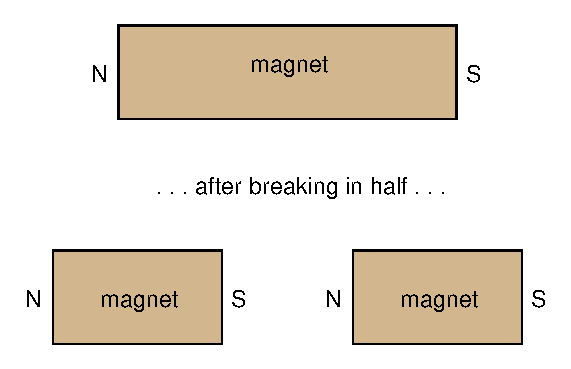
\includegraphics{../00302.eps}
%\caption{Even if the magnet is cut into tiny pieces, each piece
%will still have both a N and a S pole. These poles always occur in
%pairs.}
%\end{center}
%\end{figure}

Magnetic fields are \textit{different} from gravitational and electric
fields. In nature, positive and negative electric charges can be found 
on their own, but you \textit{never} find just a north magnetic pole or south magnetic pole on its
own. On the very small scale, zooming in to the size of atoms, magnetic fields are caused by
moving charges (i.e. the negatively charged electrons).


\subsection{Magnetic attraction and repulsion}

Like (identical) poles of magnets repel one another whilst unlike (opposite) poles attract. This means that two N poles or two S poles will push away from each other while a N
pole and a S pole will be drawn towards each other.

\Definition{Attraction and Repulsion}{\textit{Like} poles of magnets \textit{repel}
each other whilst \textit{unlike} poles \textit{attract} each other.}

\begin{wex}{Attraction and Repulsion}{Do you think the following magnets will repel or be attracted to each other?
\begin{center}
\begin{pspicture}(-0.6,0)(7.6,1)
%\psgrid[gridcolor=gray]
\psframe[fillcolor=lightgray,fillstyle=solid](0,0)(3,1)
\rput(1.5,0.5){magnet} \uput[l](0,0.5){S} \uput[r](3,0.5){N}

\rput(4,0){
\psframe[fillcolor=lightgray,fillstyle=solid](0,0)(3,1)
\rput(1.5,0.5){magnet} \uput[l](0,0.5){N} \uput[r](3,0.5){S} }
\end{pspicture}
\end{center}
}{\westep{Determine what is required} We are required to determine
whether the two magnets will repel each other or be attracted to
each other. 
\westep{Determine what is given} We are given two
magnets with the N pole of one approaching the N pole of the
other. 
\westep{Determine the conclusion} Since both poles are the same, the magnets will repel each other.}
\end{wex}

\begin{wex}{Attraction and repulsion}{Do you think the following magnets will repel or be attracted to each other?
\begin{center}
\begin{pspicture}(-0.6,0)(7.6,1)
%\psgrid[gridcolor=gray]
\psframe[fillcolor=lightgray,fillstyle=solid](0,0)(3,1)
\rput(1.5,0.5){magnet} \uput[l](0,0.5){N} \uput[r](3,0.5){S}

\rput(4,0){
\psframe[fillcolor=lightgray,fillstyle=solid](0,0)(3,1)
\rput(1.5,0.5){magnet} \uput[l](0,0.5){N} \uput[r](3,0.5){S} }
\end{pspicture}
\end{center}
}{\westep{Determine what is required} We are required to determine
whether the two magnets will repel each other or be attracted to
each other. \westep{Determine what is given} We are given two
magnets with the N pole of one approaching the S pole of the
other. \westep{Determine the conclusion} Since both poles are the
different, the magnets will be attracted to each other. }
\end{wex}


\subsection{Representing magnetic fields}

Magnetic fields can be \textit{represented} using \textbf{magnetic field lines} starting at the North pole and ending at the South pole. Although the magnetic field of a permanent magnet is everywhere surrounding the
magnet (in all three dimensions), we draw only some of the field lines to represent the field 
(usually only a two-dimensional cross-section is shown in drawings).

\begin{center}
%\scalebox{1} % Change this value to rescale the drawing.
%{
\begin{pspicture}(0,-4.62)(11.6,4.62)
\definecolor{color60}{rgb}{0.6,0.6,0.6}
\pspolygon[linewidth=0.04,fillstyle=solid](2.6,-0.8)(2.58,-1.46)(3.6,-1.48)(3.6,-0.8)
\psbezier[linewidth=0.04,linecolor=color60,arrowsize=0.05291667cm 3.0,arrowlength=1.45,arrowinset=0.3]{->}(2.02,0.78)(0.38,1.44)(1.8,-3.28)(2.9368422,-1.2441442)
\psbezier[linewidth=0.04,linecolor=color60,arrowsize=0.05291667cm 3.0,arrowlength=1.45,arrowinset=0.3]{->}(2.38,0.98)(2.9,0.88)(4.96,-3.4)(3.26,-1.24)
\psline[linewidth=0.04cm](1.78,0.6)(2.6,-1.48)
\psline[linewidth=0.04cm](1.78,1.16)(2.6,-0.78)
\psline[linewidth=0.04cm](2.66,1.16)(3.6,-0.78)
\psline[linewidth=0.04cm](1.78,0.58)(1.78,1.18)
\psline[linewidth=0.04cm](1.76,1.16)(2.68,1.16)
\psbezier[linewidth=0.04,linecolor=color60,arrowsize=0.05291667cm 3.0,arrowlength=1.45,arrowinset=0.3]{->}(2.36,1.0)(4.06,1.3)(5.7,-1.62)(3.42,-1.28)
\psbezier[linewidth=0.04,linecolor=color60,arrowsize=0.05291667cm 3.0,arrowlength=1.45,arrowinset=0.3]{->}(2.02,1.0)(0.0,1.12)(0.66,-1.82)(2.98,-1.2)
\psbezier[linewidth=0.04,linecolor=color60,arrowsize=0.05291667cm 3.0,arrowlength=1.45,arrowinset=0.3]{->}(2.2,0.88)(0.6,0.3)(3.74,-3.72)(3.08,-1.22)
\pspolygon[linewidth=0.04,fillstyle=solid](1.78,1.18)(2.6,-0.78)(3.6,-0.82)(2.64,1.16)
\pspolygon[linewidth=0.04,fillstyle=solid](1.8,1.14)(1.78,0.58)(2.58,-1.44)(2.6,-0.76)
\psbezier[linewidth=0.04,linecolor=color60,arrowsize=0.05291667cm 3.0,arrowlength=1.45,arrowinset=0.3]{->}(2.04,1.1833725)(0.98,3.34)(2.74,-1.14)(2.98,-1.1)
\psbezier[linewidth=0.04,linecolor=color60,arrowsize=0.1029cm 3.0,arrowlength=1.45,arrowinset=0.3]{->}(2.1990564,1.1633725)(1.8799998,4.36)(4.2,-1.48)(3.1301887,-1.12)
\psbezier[linewidth=0.04,linecolor=color60,arrowsize=0.05291667cm 3.0,arrowlength=1.45,arrowinset=0.3]{->}(2.42,1.1768701)(3.24,3.4199998)(4.6,-1.1)(3.44,-1.0804563)
\psbezier[linewidth=0.04](3.0626009,-0.43790242)(2.9515574,-0.425011)(2.8921053,-0.5003225)(2.938108,-0.5598407)(2.9841106,-0.6193589)(3.0651858,-0.54787487)(3.112593,-0.6178632)(3.16,-0.6878514)(3.0556846,-0.76)(2.9288561,-0.7095707)
\psline[linewidth=0.04cm](2.2,0.84)(2.08,1.1)
\psline[linewidth=0.04cm](2.08,1.1)(2.4,0.86)
\psline[linewidth=0.04cm](2.4,0.86)(2.28,1.12)
\psbezier[linewidth=0.04,linecolor=color60](8.66,1.24)(9.7295,2.68)(10.04,-2.62)(8.67725,-1.46)
\psbezier[linewidth=0.04,linecolor=color60](8.08,1.24)(7.0105,2.68)(6.7,-2.62)(8.06275,-1.46)
\psbezier[linewidth=0.04,linecolor=color60](8.54,1.22)(10.28,3.34)(10.74,-3.22)(8.54,-1.48)
\psbezier[linewidth=0.04,linecolor=color60](8.22,1.24)(6.48,3.4)(6.04,-3.18)(8.18,-1.48)
\psbezier[linewidth=0.04,linecolor=color60](8.46,1.22)(11.2,4.58)(11.58,-4.6)(8.46,-1.48)
\psbezier[linewidth=0.04,linecolor=color60](8.3,1.24)(5.56,4.6)(5.18,-4.58)(8.3,-1.46)
\psbezier[linewidth=0.04,linecolor=color60](8.44,-1.46)(8.546843,-2.750782)(10.427368,-3.02)(10.8,-2.530365)
\psbezier[linewidth=0.04,linecolor=color60](8.3,-1.46)(8.193157,-2.750782)(6.46,-2.9)(6.06,-2.5)
\psbezier[linewidth=0.04,linecolor=color60,arrowsize=0.05291667cm 3.0,arrowlength=1.4,arrowinset=0.25]{->}(8.34,1.2)(8.233157,2.490782)(6.5,2.64)(6.1,2.24)
\psbezier[linewidth=0.04,linecolor=color60,arrowsize=0.05291667cm 3.0,arrowlength=1.4,arrowinset=0.25]{->}(8.46,1.2)(8.566843,2.490782)(10.447369,2.76)(10.82,2.270365)
\psbezier[linewidth=0.04,linecolor=color60](8.38,-1.48)(8.506843,-2.790782)(9.16,-3.0)(10.2,-3.14)
\psbezier[linewidth=0.04,linecolor=color60,arrowsize=0.05291667cm 3.0,arrowlength=1.4,arrowinset=0.25]{<-}(8.36,-1.46)(8.233157,-2.770782)(7.58,-2.98)(6.54,-3.12)
\psbezier[linewidth=0.04,linecolor=color60,arrowsize=0.05291667cm 3.0,arrowlength=1.4,arrowinset=0.25]{->}(8.36,1.22)(8.233157,2.530782)(7.58,2.74)(6.54,2.88)
\psbezier[linewidth=0.04,linecolor=color60,arrowsize=0.05291667cm 3.0,arrowlength=1.4,arrowinset=0.25]{->}(8.42,1.22)(8.546843,2.530782)(9.2,2.74)(10.24,2.88)
\psline[linewidth=0.04cm,linecolor=color60,arrowsize=0.05291667cm 3.0,arrowlength=1.4,arrowinset=0.25]{->}(8.4,1.22)(8.4,3.4)
\psline[linewidth=0.04cm,linecolor=color60,arrowsize=0.05291667cm 2.0,arrowlength=1.4,arrowinset=0.4]{->}(8.36,-3.62)(8.36,-1.44)
\psbezier[linewidth=0.04](8.497481,-1.0359435)(8.393408,-0.9951322)(8.3167,-1.0527716)(8.345984,-1.1220613)(8.375269,-1.1913509)(8.471907,-1.1429322)(8.499876,-1.2227037)(8.527846,-1.3024751)(8.408568,-1.3456036)(8.298816,-1.2644686)
\psline[linewidth=0.04cm](8.28,1.12)(8.28,0.78)
\psline[linewidth=0.04cm](8.28,1.12)(8.5,0.8)
\psline[linewidth=0.04cm](8.5,0.8)(8.5,1.1)
\psbezier[linewidth=0.04,linecolor=color60,arrowsize=0.05291667cm 3.0,arrowlength=1.4,arrowinset=0.25]{<-}(8.1,-2.4)(7.72,-3.0)(6.9,-3.04)(6.54,-3.14)
\psbezier[linewidth=0.04,linecolor=color60,arrowsize=0.05291667cm 3.0,arrowlength=1.4,arrowinset=0.25]{<-}(7.68,-2.4733334)(7.14,-2.78)(6.24,-2.74)(6.06,-2.48)
\psline[linewidth=0.04cm,linecolor=color60,arrowsize=0.05291667cm 3.0,arrowlength=1.4,arrowinset=0.25]{->}(8.36,-3.52)(8.36,-2.44)
\psbezier[linewidth=0.04,linecolor=color60,arrowsize=0.05291667cm 3.0,arrowlength=1.4,arrowinset=0.25]{<-}(8.82,-2.54)(8.92,-2.82)(9.7,-3.14)(10.18,-3.12)
\psbezier[linewidth=0.04,linecolor=color60,arrowsize=0.05291667cm 3.0,arrowlength=1.4,arrowinset=0.25]{<-}(9.12,-2.46)(9.46,-2.74)(10.46,-2.9)(10.82,-2.54)
\psbezier[linewidth=0.04,linecolor=color60,arrowsize=0.05291667cm 3.0,arrowlength=1.4,arrowinset=0.25]{->}(8.66,1.24)(9.38,2.18)(9.58,0.22)(9.58,-0.22)
\psbezier[linewidth=0.04,linecolor=color60,arrowsize=0.05291667cm 3.0,arrowlength=1.4,arrowinset=0.25]{->}(8.56,1.22)(9.7,2.52)(9.98,0.5)(10.06,-0.2)
\psbezier[linewidth=0.04,linecolor=color60,arrowsize=0.05291667cm 3.0,arrowlength=1.4,arrowinset=0.25]{->}(8.46,1.24)(10.18,3.22)(10.66,0.66)(10.66,-0.2)
\psbezier[linewidth=0.04,linecolor=color60,arrowsize=0.05291667cm 3.0,arrowlength=1.4,arrowinset=0.25]{->}(8.08,1.24)(7.34,2.14)(7.16,0.24)(7.16,-0.22)
\psbezier[linewidth=0.04,linecolor=color60,arrowsize=0.05291667cm 3.0,arrowlength=1.4,arrowinset=0.25]{->}(8.22,1.24)(6.94,2.66)(6.74,0.2)(6.78,-0.22)
\psbezier[linewidth=0.04,linecolor=color60,arrowsize=0.05291667cm 3.0,arrowlength=1.4,arrowinset=0.25]{->}(8.28,1.26)(6.5,3.3)(6.08,0.5)(6.1,-0.26)
\psframe[linewidth=0.04,dimen=outer](8.9,1.24)(7.86,-1.5)
\rput(2.851875,-2.47){3-dimensional representation}
\rput(8.415313,-3.89){2-dimensional representation}
\end{pspicture} 
%}
\end{center}

In areas where the magnetic field is strong, the field lines are closer together. 
Where the field is weaker, the field lines are drawn further apart. The number of field lines drawn crossing a given two-dimensional surface is referred to as the \textbf{magnetic flux}. The magnetic flux is used as a measure of the strength of the magnetic field over that surface.
\Tip{
\begin{enumerate}
\item Field lines \textit{never} cross.
\item Arrows drawn on the field lines indicate the direction of the field.  
\item A magnetic field points from the north to the south
pole of a magnet. 
\end{enumerate}
}


\Activity{Investigation}{Field around a Bar Magnet}{Take a bar magnet and place
it on a flat surface. Place a sheet of white paper over the bar
magnet and sprinkle some iron filings onto the paper. Give the
paper a shake to evenly distribute the iron filings. In your
workbook, draw the bar magnet and the pattern formed by the iron
filings. Draw the pattern formed when you rotate the bar magnet to a different angle as
shown below.

\begin{center}
\begin{pspicture}(-0.6,-0.2)(5.2,5.2)
%\psgrid[gridcolor=gray]
\def\magnet{\psset{unit=0.75}\psframe[fillcolor=lightgray,fillstyle=solid](0,0)(3,1)
\rput(1.5,0.5){magnet} \uput[l](0,0.5){N} \uput[r](3,0.5){S} }
\rput(0,0.5){\magnet} \rput{45}(3.5,0){\magnet}
\rput{-45}(0,4){\magnet} \rput{90}(3.5,2.5){\magnet}
\end{pspicture}
\end{center}
}

%The magnetic field around a permanent bar magnet is shown in
%Figure~\ref{fig:p:em:m10:field1}.

%\begin{figure}[htbp]
%\begin{center}
%\begin{pspicture}(0,0)(5,5)
%\psgrid[gridcolor=gray]
%\rput(2.5,2.5){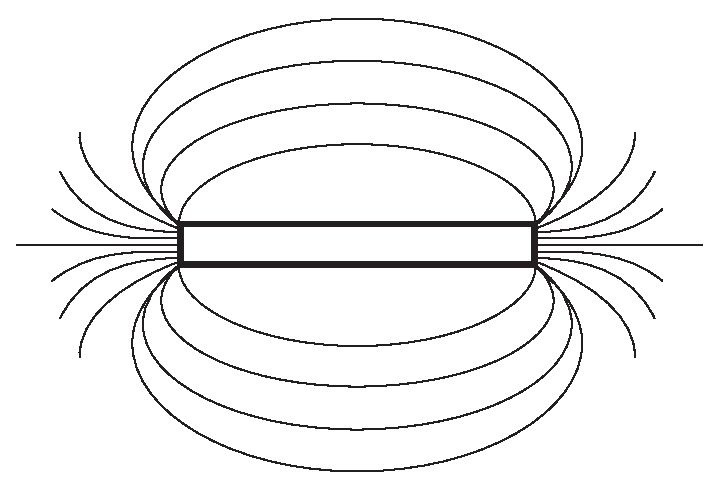
\includegraphics[width=7.5cm]{../magnet.eps}}
%\rput(1,2.5){N} \rput(4,2.5){S} \psline{->}(2.4,3.6)(2.6,3.6)
%\psline{->}(2.4,4.05)(2.6,4.05) \psline{->}(2.4,4.515)(2.6,4.515)
%\psline{->}(2.4,4.96)(2.6,4.96) \psline{->}(2.4,1.4)(2.6,1.4)
%\psline{->}(2.4,0.95)(2.6,0.95) \psline{->}(2.4,0.485)(2.6,0.485)
%\psline{->}(2.4,0.04)(2.6,0.04)
%\end{pspicture}
%\caption{The magnetic field around a permanent bar magnet is
%shown. Lines are usually drawn emerging from the North pole of the
%magnet.} \label{fig:p:em:m10:field1}
%\end{center}
%\end{figure}

As the activity shows, one can map the magnetic field of a magnet by 
placing it underneath a piece of paper and sprinkling
iron filings on top. The iron filings line themselves up parallel to the magnetic field.\\ 



\Activity{Investigation}{Field around a Pair of Bar Magnets}{Take two bar magnets
and place them a short distance apart such that they are repelling
each other. Place a sheet of white paper over the bar magnets and
sprinkle some iron filings onto the paper. Give the paper a shake
to evenly distribute the iron filings. In your workbook, draw both
the bar magnets and the pattern formed by the iron filings. Repeat
the procedure for two bar magnets attracting each other and draw
what the pattern looks like for this situation. Make a note of the
shape of the lines formed by the iron filings, as well as their
size and their direction for both arrangements of the bar magnet.
What does the pattern look like when you place both bar magnets
side by side?

\begin{center}
\begin{pspicture}(-0.6,-1)(7.4,6.6)
%\psgrid[gridcolor=gray]
\def\magnet{\psframe[fillcolor=lightgray,fillstyle=solid](0,0)(3,1)
\rput(1.5,0.5){magnet} \uput[l](0,0.5){N} \uput[r](3,0.5){S}}

\def\reversedmagnet{\psframe[fillcolor=lightgray,fillstyle=solid](0,0)(3,1)
\rput(1.5,0.5){magnet} \uput[l](0,0.5){S} \uput[r](3,0.5){N}}


\rput(0,5.5){ \rput(0,0){\magnet} \rput(4,0){\magnet}}
\uput[l](-0.6,6){Arrangement 1}

\rput(0,4){ \rput(0,0){\reversedmagnet} \rput(4,0){\magnet}}
\uput[l](-0.6,4.5){Arrangement 2}

\rput(1.25,0){ \rput{90}(0,0){\magnet} \rput{90}(1.5,0){\magnet} }
\uput[d](1.5,-0.6){Arrangement 3}

\rput(5.25,0){ \rput{90}(0,0){\magnet}
\rput{90}(1.5,0){\reversedmagnet} } \uput[d](5.5,-0.6){Arrangement
4}

\end{pspicture}
\end{center}
}

As already said, opposite poles of a magnet attract each other and
bringing them together causes their magnetic field lines to
\textit{converge} (come together). Like poles of a magnet repel each other and bringing
them together causes their magnetic field lines to \textit{diverge} (bend out from each other).

\begin{center}
\scalebox{1} % Change this value to rescale the drawing.
{
\begin{pspicture}(0,-2.3739064)(10.2,2.3739064)
\psframe[linewidth=0.04,dimen=outer](3.62,0.50390625)(0.0,-0.45609376)
\psframe[linewidth=0.04,dimen=outer](10.2,0.50390625)(6.58,-0.45609376)
\psbezier[linewidth=0.04,arrowsize=0.05291667cm 3.0,arrowlength=1.4,arrowinset=0.3]{->}(3.62,0.10390625)(4.12,0.10390625)(4.92,0.32390624)(4.8940845,1.9039062)
\psbezier[linewidth=0.04,arrowsize=0.05291667cm 3.0,arrowlength=1.4,arrowinset=0.3]{->}(6.6,0.10390625)(6.1,0.10390625)(5.2,0.46390626)(5.34,1.9239062)
\psbezier[linewidth=0.04,arrowsize=0.05291667cm 3.0,arrowlength=1.4,arrowinset=0.3]{->}(3.6,-0.03609375)(4.1,-0.03609375)(4.9,-0.22240955)(4.8740845,-1.8360938)
\psbezier[linewidth=0.04,arrowsize=0.05291667cm 3.0,arrowlength=1.4,arrowinset=0.3]{->}(6.62,-0.03609375)(6.12,-0.03609375)(5.22,-0.39609376)(5.36,-1.8560938)
\psbezier[linewidth=0.04,arrowsize=0.05291667cm 3.0,arrowlength=1.4,arrowinset=0.3]{->}(3.6,0.20390625)(4.0827584,0.20390625)(4.76,0.68390626)(4.5655174,1.8039062)
\psbezier[linewidth=0.04,arrowsize=0.05291667cm 3.0,arrowlength=1.4,arrowinset=0.3]{->}(3.6,-0.11609375)(4.0827584,-0.11609375)(4.76,-0.5960938)(4.5655174,-1.7160938)
\psbezier[linewidth=0.04,arrowsize=0.05291667cm 3.0,arrowlength=1.4,arrowinset=0.3]{->}(6.62,0.18390626)(6.1372414,0.18390626)(5.46,0.6639063)(5.654483,1.7839062)
\psbezier[linewidth=0.04,arrowsize=0.05291667cm 3.0,arrowlength=1.4,arrowinset=0.3]{->}(6.62,-0.11609375)(6.1372414,-0.11609375)(5.46,-0.5960938)(5.654483,-1.7160938)
\psbezier[linewidth=0.04,arrowsize=0.05291667cm 3.0,arrowlength=1.4,arrowinset=0.3]{->}(3.58,0.30390626)(3.934138,0.30390626)(4.68,0.8383507)(4.288276,1.7839062)
\psbezier[linewidth=0.04,arrowsize=0.05291667cm 3.0,arrowlength=1.4,arrowinset=0.3]{->}(3.58,-0.19609375)(3.934138,-0.19609375)(4.68,-0.7305382)(4.288276,-1.6760937)
\psbezier[linewidth=0.04,arrowsize=0.05291667cm 3.0,arrowlength=1.4,arrowinset=0.3]{->}(6.62,-0.21609375)(6.265862,-0.21609375)(5.52,-0.7505382)(5.9117236,-1.6960938)
\psbezier[linewidth=0.04,arrowsize=0.05291667cm 3.0,arrowlength=1.4,arrowinset=0.3]{->}(6.62,0.28390625)(6.265862,0.28390625)(5.52,0.8183507)(5.9117236,1.7639062)
\psbezier[linewidth=0.04,arrowsize=0.05291667cm 3.0,arrowlength=1.4,arrowinset=0.3]{->}(3.62,0.40390626)(4.12,0.6039063)(4.48,1.0439062)(3.94,1.7039063)
\psbezier[linewidth=0.04,arrowsize=0.05291667cm 3.0,arrowlength=1.4,arrowinset=0.3]{->}(3.62,-0.29609376)(4.12,-0.49609375)(4.48,-0.93609375)(3.94,-1.5960938)
\psbezier[linewidth=0.04,arrowsize=0.05291667cm 3.0,arrowlength=1.4,arrowinset=0.3]{->}(6.62,-0.29609376)(6.12,-0.49609375)(5.76,-0.93609375)(6.3,-1.5960938)
\psbezier[linewidth=0.04,arrowsize=0.05291667cm 3.0,arrowlength=1.4,arrowinset=0.3]{->}(6.62,0.34390625)(6.12,0.5439063)(5.76,0.98390627)(6.3,1.6439062)
\rput(3.2696877,-0.02609375){N}
\rput(6.929688,-0.00609375){N}
\rput(0.2584375,-0.00609375){S}
\rput(9.858438,-0.02609375){S}
\rput(5.115,2.1939063){Like poles repel each other}
\rput(5.17875,-2.1460938){The field lines between 2 like poles diverge}
\end{pspicture} 
}
\end{center}

\begin{center}
\scalebox{1} % Change this value to rescale the drawing.
{
\begin{pspicture}(0,-2.0239062)(10.2,2.0239062)
\psframe[linewidth=0.04,dimen=outer](3.62,0.45390618)(0.0,-0.5060938)
\psframe[linewidth=0.04,dimen=outer](10.2,0.45390618)(6.58,-0.5060938)
\rput(3.2696877,-0.0760938){N}
\rput(6.8584375,-0.0560938){S}
\rput(0.2584375,-0.0560938){S}
\rput(9.9296875,-0.0760938){N}
\rput(5.2503123,1.8439063){Unlike poles attract each other}
\psline[linewidth=0.04cm,arrowsize=0.05291667cm 3.0,arrowlength=1.4,arrowinset=0.3]{->}(3.6,-0.0260938)(6.6,-0.0460938)
\psbezier[linewidth=0.04,arrowsize=0.05291667cm 3.0,arrowlength=1.4,arrowinset=0.3]{->}(3.58,0.0539062)(4.208322,0.5139062)(5.96,0.4939062)(6.6,0.0939062)
\psbezier[linewidth=0.04,arrowsize=0.05291667cm 3.0,arrowlength=1.4,arrowinset=0.3]{->}(3.6,-0.1060938)(4.228322,-0.5660938)(5.98,-0.5460938)(6.62,-0.14609382)
\psbezier[linewidth=0.04,arrowsize=0.05291667cm 3.0,arrowlength=1.4,arrowinset=0.3]{->}(3.58,0.21390618)(4.22,1.0739063)(5.96,1.0139061)(6.6,0.2539062)
\psbezier[linewidth=0.04,arrowsize=0.05291667cm 3.0,arrowlength=1.4,arrowinset=0.3]{->}(3.62,-0.1860938)(4.26,-1.0460937)(6.0,-0.9860938)(6.64,-0.2260938)
\psbezier[linewidth=0.04,arrowsize=0.05291667cm 3.0,arrowlength=1.4,arrowinset=0.3]{->}(3.6,0.4139062)(4.42,1.7739061)(5.74,1.8139062)(6.62,0.45390618)
\psbezier[linewidth=0.04,arrowsize=0.05291667cm 3.0,arrowlength=1.4,arrowinset=0.3]{->}(3.6,-0.3460938)(4.42,-1.7060939)(5.74,-1.7460939)(6.62,-0.3860938)
\rput(5.09875,-1.7960937){The magnetic field lines between 2 unlike poles converge}
\end{pspicture} 
}
\end{center}



\Extension{Ferromagnetism and Retentivity}{
\textbf{Ferromagnetism} is a
phenomenon shown by materials like iron, nickel or cobalt.
These materials can form permanent magnets. They always
magnetise so as to be attracted to a magnet, no matter which
magnetic pole is brought toward the unmagnetised iron/nickel/cobalt.

\noindent The ability of a ferromagnetic material to retain its
magnetisation \textit{after} an external field is removed is called its
\textbf{retentivity}. 

\noindent \textbf{Paramagnetic} materials are materials like
aluminium or platinum, which become magnetised in an external
magnetic field in a similar way to ferromagnetic materials. However, they
lose their magnetism when the external magnetic field is removed.

\noindent \textbf{Diamagnetism} is shown by materials like copper or bismuth,
which become magnetised in a magnetic field with a polarity
\textit{opposite} to the external magnetic field. Unlike iron, they are
slightly repelled by a magnet.
}

\section{The compass and the earth's magnetic field}

A \textbf{compass} is an instrument which is used to find the direction of a 
magnetic
field. A compass consists of a small metal needle which
is magnetised itself and which is free to turn in any direction. 
Therefore, when in the presence of a magnetic field, 
the needle is able to line up in the same direction as the field. 


\begin{center}
%\scalebox{1} % Change this value to rescale the drawing.
%{
\begin{pspicture}(0,-3.4589062)(6.0834374,3.4389062)
\definecolor{color60}{rgb}{0.6,0.6,0.6}
\psbezier[linewidth=0.04,linecolor=color60](3.2359998,0.9866473)(4.0514936,2.029044)(4.28825,-1.807555)(3.249153,-0.9678465)
\psbezier[linewidth=0.04,linecolor=color60](2.7937498,0.9866473)(1.9782562,2.029044)(1.7414999,-1.807555)(2.7805967,-0.9678465)
\psbezier[linewidth=0.04,linecolor=color60](3.1444998,0.9721696)(4.47125,2.5068092)(4.822,-2.2418869)(3.1444998,-0.98232424)
\psbezier[linewidth=0.04,linecolor=color60](2.9004998,0.9866473)(1.5737499,2.5502424)(1.23825,-2.2129314)(2.87,-0.98232424)
\psbezier[linewidth=0.04,linecolor=color60](3.0835,0.9721696)(5.17275,3.4044285)(5.4624996,-3.2408504)(3.0835,-0.98232424)
\psbezier[linewidth=0.04,linecolor=color60](2.9615,0.9866473)(0.87224996,3.4189062)(0.5825,-3.2263727)(2.9615,-0.9678465)
\psbezier[linewidth=0.04,linecolor=color60](3.06825,-0.9678465)(3.1497178,-1.9022263)(4.583618,-2.0971096)(4.8677497,-1.7426693)
\psbezier[linewidth=0.04,linecolor=color60](2.9615,-0.9678465)(2.880032,-1.9022263)(1.5584999,-2.0102432)(1.2535,-1.7206886)
\psbezier[linewidth=0.04,linecolor=color60,arrowsize=0.05291667cm 3.0,arrowlength=1.4,arrowinset=0.25]{->}(2.9919999,0.95769185)(2.910532,1.8920717)(1.589,2.0000885)(1.2839999,1.7105339)
\psbezier[linewidth=0.04,linecolor=color60,arrowsize=0.05291667cm 3.0,arrowlength=1.4,arrowinset=0.25]{->}(3.0835,0.95769185)(3.1649678,1.8920717)(4.5988684,2.0869548)(4.883,1.7325147)
\psbezier[linewidth=0.04,linecolor=color60](3.0224998,-0.98232424)(3.1192176,-1.9311818)(3.61725,-2.0826318)(4.4102497,-2.183976)
\psbezier[linewidth=0.04,linecolor=color60,arrowsize=0.05291667cm 3.0,arrowlength=1.4,arrowinset=0.25]{<-}(3.0072498,-0.9678465)(2.910532,-1.916704)(2.4125,-2.068154)(1.6194999,-2.1694982)
\psbezier[linewidth=0.04,linecolor=color60,arrowsize=0.05291667cm 3.0,arrowlength=1.4,arrowinset=0.25]{->}(3.0072498,0.9721696)(2.910532,1.9210272)(2.4125,2.072477)(1.6194999,2.1738212)
\psbezier[linewidth=0.04,linecolor=color60,arrowsize=0.05291667cm 3.0,arrowlength=1.4,arrowinset=0.25]{->}(3.053,0.9721696)(3.1497178,1.9210272)(3.64775,2.072477)(4.4407496,2.1738212)
\psline[linewidth=0.04cm,linecolor=color60,arrowsize=0.05291667cm 3.0,arrowlength=1.4,arrowinset=0.25]{->}(3.03775,0.9721696)(3.03775,2.5502424)
\psline[linewidth=0.04cm,linecolor=color60,arrowsize=0.05291667cm 2.0,arrowlength=1.4,arrowinset=0.4]{->}(3.0072498,-2.5314415)(3.0072498,-0.9533688)
\psbezier[linewidth=0.04](3.1120791,-0.6608777)(3.0327232,-0.6313349)(2.9742334,-0.6730593)(2.9965632,-0.7232172)(3.0188928,-0.7733751)(3.0925786,-0.7383254)(3.1139057,-0.7960709)(3.1352324,-0.85381633)(3.0442836,-0.88503647)(2.9605973,-0.82630384)
\psline[linewidth=0.04cm](2.94625,0.8997809)(2.94625,0.65365946)
\psline[linewidth=0.04cm](2.94625,0.8997809)(3.1139998,0.6681372)
\psline[linewidth=0.04cm](3.1139998,0.6681372)(3.1139998,0.8853032)
\psbezier[linewidth=0.04,linecolor=color60,arrowsize=0.05291667cm 3.0,arrowlength=1.4,arrowinset=0.25]{<-}(2.809,-1.6482999)(2.51925,-2.0826318)(1.8939999,-2.1115873)(1.6194999,-2.183976)
\psbezier[linewidth=0.04,linecolor=color60,arrowsize=0.05291667cm 3.0,arrowlength=1.4,arrowinset=0.25]{<-}(2.48875,-1.7013849)(2.077,-1.9233768)(1.3907499,-1.8944213)(1.2535,-1.7062109)
\psline[linewidth=0.04cm,linecolor=color60,arrowsize=0.05291667cm 3.0,arrowlength=1.4,arrowinset=0.25]{->}(3.0072498,-2.4590528)(3.0072498,-1.6772554)
\psbezier[linewidth=0.04,linecolor=color60,arrowsize=0.05291667cm 3.0,arrowlength=1.4,arrowinset=0.25]{<-}(3.3579998,-1.749644)(3.4342499,-1.9523323)(4.029,-2.183976)(4.395,-2.1694982)
\psbezier[linewidth=0.04,linecolor=color60,arrowsize=0.05291667cm 3.0,arrowlength=1.4,arrowinset=0.25]{<-}(3.5867498,-1.6917331)(3.846,-1.8944213)(4.6085,-2.0102432)(4.883,-1.749644)
\psbezier[linewidth=0.04,linecolor=color60,arrowsize=0.05291667cm 3.0,arrowlength=1.4,arrowinset=0.25]{->}(3.2359998,0.9866473)(3.7849998,1.6671007)(3.9374998,0.24828297)(3.9374998,-0.070227124)
\psbezier[linewidth=0.04,linecolor=color60,arrowsize=0.05291667cm 3.0,arrowlength=1.4,arrowinset=0.25]{->}(3.15975,0.9721696)(4.029,1.9132222)(4.2425,0.45097122)(4.3034997,-0.055749394)
\psbezier[linewidth=0.04,linecolor=color60,arrowsize=0.05291667cm 3.0,arrowlength=1.4,arrowinset=0.25]{->}(3.0835,0.9866473)(4.395,2.4199429)(4.7609997,0.5667931)(4.7609997,-0.055749394)
\psbezier[linewidth=0.04,linecolor=color60,arrowsize=0.05291667cm 3.0,arrowlength=1.4,arrowinset=0.25]{->}(2.7937498,0.9866473)(2.2294998,1.6381452)(2.0922499,0.2627607)(2.0922499,-0.070227124)
\psbezier[linewidth=0.04,linecolor=color60,arrowsize=0.05291667cm 3.0,arrowlength=1.4,arrowinset=0.25]{->}(2.9004998,0.9866473)(1.9245,2.0145662)(1.772,0.23380524)(1.8024999,-0.070227124)
\psbezier[linewidth=0.04,linecolor=color60,arrowsize=0.05291667cm 3.0,arrowlength=1.4,arrowinset=0.25]{->}(2.94625,1.001125)(1.589,2.4778538)(1.26875,0.45097122)(1.2839999,-0.09918259)
\psframe[linewidth=0.04,dimen=outer](3.419,0.9866473)(2.626,-0.996802)
\pscircle[linewidth=0.078,dimen=outer](5.5125,-0.03109375){0.51}
\pspolygon[linewidth=0.04,fillstyle=solid,fillcolor=black](5.443904,-0.00109375)(5.443904,-0.23806344)(5.3425,-0.22316271)(5.5087137,-0.46109375)(5.6425,-0.24462315)(5.571286,-0.2392114)(5.578153,-0.00109375)
\pscircle[linewidth=0.04,linecolor=white,dimen=outer,fillstyle=solid](5.5025,-0.04109375){0.02}
\pscircle[linewidth=0.078,dimen=outer](0.5125,-0.03109375){0.51}
\pspolygon[linewidth=0.04,fillstyle=solid,fillcolor=black](0.44390392,-0.00109375)(0.44390392,-0.23806344)(0.3425,-0.22316271)(0.50871384,-0.46109375)(0.6425,-0.24462315)(0.57128626,-0.2392114)(0.578153,-0.00109375)
\pscircle[linewidth=0.04,linecolor=white,dimen=outer,fillstyle=solid](0.5025,-0.04109375){0.02}
\rput{-79.904144}(6.0744042,3.309316){\pscircle[linewidth=0.078,dimen=outer,fillstyle=solid](5.0125,-1.9710938){0.51}}
\pspolygon[linewidth=0.04,fillstyle=solid,fillcolor=black](5.0300107,-1.898301)(4.7967105,-1.9398407)(4.793605,-1.8373948)(4.5884943,-2.0427432)(4.825065,-2.1365116)(4.8179097,-2.0654519)(5.053544,-2.0304713)
\rput{-79.904144}(6.0568724,3.304571){\pscircle[linewidth=0.04,linecolor=white,dimen=outer,fillstyle=solid](5.0009017,-1.9630015){0.02}}
\rput{-101.33104}(0.30287695,4.786019){\pscircle[linewidth=0.078,dimen=outer,fillstyle=solid](2.1125,2.2689064){0.51}}
\pspolygon[linewidth=0.04,fillstyle=solid,fillcolor=black](2.155393,2.330271)(1.923042,2.37683)(1.9575759,2.4733298)(1.6916254,2.3571038)(1.8775905,2.183394)(1.8968887,2.2521563)(2.129016,2.1986387)
\rput{-101.33104}(0.28195578,4.7924137){\pscircle[linewidth=0.04,linecolor=white,dimen=outer,fillstyle=solid](2.1046598,2.2806761){0.02}}
\rput(3.0170312,-2.8310938){The direction of the compass arrow is the }
\rput(3.0042188,-3.2310936){same as the direction of the magnetic field}
\end{pspicture} 
%}
\end{center}

\begin{IFact}
{Lodestone, a magnetised form of iron-oxide, was found to orientate itself 
in a north-south direction if left free to rotate by suspension
on a string or on a float in water. Lodestone was therefore used as 
an early navigational compass.
}
\end{IFact}

Compasses are mainly used in navigation to find direction on the earth. 
This works because 
the earth itself has a magnetic field which is similar to that of a bar magnet
(see the picture below). The compass needle aligns with the earth's magnetic field
direction and points north-south. Once you know where north is, you can 
figure out any other direction. A picture of a compass is shown below:

\begin{center}
\scalebox{1} % Change this value to rescale the drawing.
{
\begin{pspicture}(0,-1.4)(6.02125,1.4)
\definecolor{color1276b}{rgb}{0.4,0.4,0.4}
\pscircle[linewidth=0.07,dimen=outer](1.4,0.0){1.3}
\rput(1.4098438,1.05){N}
\rput(1.3792187,-1.05){S}
\rput(0.40609375,0.01){W}
\rput(2.4020312,0.01){E}
\pscircle[linewidth=0.07,dimen=outer](1.4,0.0){1.4}
\rput(0.79296875,0.725){\scriptsize NW}
\rput(2.0842187,0.725){\scriptsize NE}
\rput(0.7423437,-0.755){\scriptsize SW}
\rput(2.0735939,-0.755){\scriptsize SE}
\psdiamond[linewidth=0.04,dimen=outer,gangle=-89.052](1.39,-0.00955629)(0.15,0.8504437)
\psline[linewidth=0.04cm](0.76,0.0)(2.14,0.0)
\psdiamond[linewidth=0.04,dimen=outer](1.4,-0.00955629)(0.18,0.9104437)
\pspolygon[linewidth=0.04,fillstyle=solid,fillcolor=color1276b](1.24,-0.0014992657)(1.4,0.80420315)(1.54,-0.0014992657)
\pscircle[linewidth=0.04,dimen=outer,fillstyle=solid,fillcolor=black](1.3844562,-0.0014992657){0.064456195}
\pspolygon[linewidth=0.04,fillstyle=solid](1.4,-0.78)(1.54,-0.02)(1.24,-0.02)
\pscircle[linewidth=0.04,dimen=outer,fillstyle=solid,fillcolor=black](1.3844562,-0.021499265){0.064456195}
\psline[linewidth=0.04cm](1.38,0.32)(3.4,0.8)
\psline[linewidth=0.04cm](1.38,0.0)(3.4,-0.42)
\rput(4.729219,0.84){\small magnetised needle}
\rput(3.798125,-0.42){\small pivot}
\end{pspicture} 
}
\end{center}

Some animals can detect magnetic fields, which
helps them orientate themselves and navigate. Animals which can do this include pigeons, bees, Monarch
butterflies, sea turtles and certain fish.

% \newpage
\subsection{The earth's magnetic field}

In the picture below, you can see a representation of the earth's magnetic
field which is very similar to the magnetic field of a giant bar magnet like
the one on the right of the picture. So the earth has two sets of north poles
and south poles: \textbf{geographic poles} and \textbf{magnetic poles}.


\begin{center}
\scalebox{0.95} % Change this value to rescale the drawing.
{
\begin{pspicture}(0,-3.7089062)(15.38,3.72)
\definecolor{color875}{rgb}{0.4,0.4,0.4}
\rput(4.08,3.59){\tiny 11.5$^{o}$}
\rput(5.80,3.08){Geographic North pole}
\rput(1.95,3.30){\color{color875}Magnetic 'North' pole}
\psbezier[linewidth=0.04,linecolor=color875,arrowsize=0.05291667cm 2.0,arrowlength=1.4,arrowinset=0.4]{->}(3.74,-1.38)(3.9,-2.10)(4.34,-2.58)(4.98,-2.90)
\psbezier[linewidth=0.04,linecolor=color875,arrowsize=0.05291667cm 2.0,arrowlength=1.4,arrowinset=0.4]{->}(3.58,-1.34)(3.1,-3.26)(1.14,-3.10)(1.02,-3.12)
\psbezier[linewidth=0.04,linecolor=color875,arrowsize=0.05291667cm 2.0,arrowlength=1.4,arrowinset=0.4]{->}(3.54,-1.40)(3.38,-2.12)(2.94,-2.60)(2.3,-2.92)
\psbezier[linewidth=0.04,linecolor=color875,arrowsize=0.05291667cm 2.0,arrowlength=1.4,arrowinset=0.4]{->}(3.54,-1.36)(2.26,-3.04)(0.6,-2.50)(0.48,-2.20)
\psbezier[linewidth=0.04,linecolor=color875,arrowsize=0.05291667cm 2.0,arrowlength=1.4,arrowinset=0.4]{->}(3.52,-1.38)(3.06,-1.96)(2.68,-2.20)(2.06,-2.46)
\psbezier[linewidth=0.04,linecolor=color875,arrowsize=0.05291667cm 3.0,arrowlength=1.4,arrowinset=0.4]{->}(3.41,-1.38)(2.05,-1.72)(1.63,-0.90)(1.59,-0.10)
\psline[linewidth=0.04cm,linecolor=color875,linestyle=dashed,dash=0.16cm 0.16cm](3.62,3.35)(3.62,-3.68)
\psline[linewidth=0.04cm](4.18,3.34)(3.11,-3.48)
\psbezier[linewidth=0.04,linecolor=color875](3.82,1.15)(5.93,2.29)(6.54,-2.14)(3.87,-1.36)
\psbezier[linewidth=0.04,linecolor=color875,arrowsize=0.05291667cm 3.0,arrowlength=1.4,arrowinset=0.4]{->}(3.90,-1.36)(5.20,-1.70)(5.61,-0.88)(5.64,-0.08)
\psbezier[linewidth=0.04,linecolor=color875](3.5,1.13)(1.29,2.27)(0.66,-2.16)(3.44,-1.38)
\psbezier[linewidth=0.04,linecolor=color875](3.7,1.15)(6.84,3.47)(7.28,-3.24)(3.76,-1.36)
\psbezier[linewidth=0.04,linecolor=color875,arrowsize=0.05291667cm 3.0,arrowlength=1.4,arrowinset=0.4]{->}(3.78,-1.38)(5.04,-2.06)(6.1,-1.64)(6.24,-0.068)
\psbezier[linewidth=0.04,linecolor=color875](3.58,1.15)(0.44,3.47)(0.0,-3.24)(3.52,-1.36)
\psbezier[linewidth=0.04,linecolor=color875,arrowsize=0.05291667cm 3.0,arrowlength=1.4,arrowinset=0.4]{->}(3.48,-1.38)(2.22,-2.06)(1.18,-1.64)(1.04,-0.048)
\psbezier[linewidth=0.04,linecolor=color875,arrowsize=0.05291667cm 2.0,arrowlength=1.4,arrowinset=0.4]{<-}(3.68,1.15)(4.16,3.07)(6.12,2.91)(6.24,2.93)
\psbezier[linewidth=0.04,linecolor=color875,arrowsize=0.05291667cm 2.0,arrowlength=1.4,arrowinset=0.4]{<-}(3.58,1.15)(3.1,3.07)(1.14,2.91)(1.02,2.93)
\psbezier[linewidth=0.04,linecolor=color875,arrowsize=0.05291667cm 2.0,arrowlength=1.4,arrowinset=0.4]{->}(3.72,-1.34)(4.2,-3.26)(6.16,-3.10)(6.28,-3.12)
\psbezier[linewidth=0.04,linecolor=color875,arrowsize=0.05291667cm 2.0,arrowlength=1.4,arrowinset=0.4]{<-}(3.76,1.15)(5.0332885,2.83)(6.7,2.29)(6.82,1.99)
\psbezier[linewidth=0.04,linecolor=color875,arrowsize=0.05291667cm 2.0,arrowlength=1.4,arrowinset=0.4]{<-}(3.56,1.15)(2.28,2.83)(0.62,2.29)(0.5,1.99)
\psbezier[linewidth=0.04,linecolor=color875,arrowsize=0.05291667cm 2.0,arrowlength=1.4,arrowinset=0.4]{->}(3.76,-1.36)(5.03,-3.04)(6.7,-2.50)(6.82,-2.20)
\psbezier[linewidth=0.04,linecolor=color875,arrowsize=0.05291667cm 2.0,arrowlength=1.4,arrowinset=0.4]{->}(6.84,2.01)(6.24,2.57)(5.053,2.23)(4.78,2.05)
\psbezier[linewidth=0.04,linecolor=color875,arrowsize=0.05291667cm 2.0,arrowlength=1.4,arrowinset=0.4]{->}(0.48,2.01)(1.08,2.57)(2.26,2.23)(2.54,2.05)
\psbezier[linewidth=0.04,linecolor=color875,arrowsize=0.05291667cm 2.0,arrowlength=1.4,arrowinset=0.4]{->}(6.24,2.93)(5.5,2.95)(4.94,2.75)(4.5,2.45)
\psbezier[linewidth=0.04,linecolor=color875,arrowsize=0.05291667cm 2.0,arrowlength=1.4,arrowinset=0.4]{->}(1.14,2.93)(1.56,2.91)(2.32,2.79)(2.8,2.43)
\psbezier[linewidth=0.04,linecolor=color875,arrowsize=0.05291667cm 2.0,arrowlength=1.4,arrowinset=0.4]{->}(3.78,-1.38)(4.24,-1.96)(4.62,-2.20)(5.24,-2.46)
\rput{-19.00}(0.23,1.16){\pscircle[linewidth=0.04,dimen=outer,fillstyle=solid](3.60,-0.11){1.29}}
\psbezier[linewidth=0.04](3.98,0.27)(3.97,0.31)(3.97,0.31)(3.97,0.32)(3.98,0.33)(3.96,0.37)(3.97,0.36)(3.98,0.35)(3.97,0.34)(3.96,0.34)(3.96,0.35)(4.01,0.36)(3.98,0.36)(3.95,0.36)(3.98,0.47)(3.72,0.45)(3.47,0.43)(3.68,0.56)(3.60,0.57)(3.51,0.58)(3.50,0.57)(3.35,0.55)(3.21,0.53)(3.09,0.52)(2.96,0.37)(2.832,0.2295)(2.731,-0.0794)(2.908,-0.1861)(3.084,-0.292)(3.310,-0.261)(3.358,-0.343)(3.406,-0.426)(3.290,-0.703)(3.383,-0.809)(3.477,-0.914)(3.425,-1.007)(3.469,-1.053)(3.513,-1.099)(3.676,-1.124)(3.738,-1.066)(3.801,-1.008)(3.855,-0.837)(3.958,-0.8094)(4.0619,-0.7816)(4.004,-0.485)(4.127,-0.434)(4.249,-0.383)(4.382,-0.238)(4.426,-0.166)(4.469,-0.0952)(4.290,-0.185)(4.173,-0.1098)(4.055,-0.0342)(3.994,0.232)(3.983,0.274)
\psbezier[linewidth=0.04](3.940,0.38)(3.92,0.18)(4.33,-0.04)(4.28,-0.045)(4.24,-0.046)(4.55,0.012)(4.52,0.17)(4.49,0.33)(4.18,0.074)(4.27,0.27)(4.36,0.47)(4.88,-0.05)(4.81,0.03)(4.74,0.11)(4.8,0.41)(4.6,0.56)(4.51,0.71)(4.24,1.14)(3.85,1.09)(3.47,1.04)(3.89,0.82)(3.58,0.93)(3.27,1.04)(3.07,0.58)(3.28,0.65)(3.48,0.72)(3.72,0.68)(3.76,0.65)(3.80,0.63)(3.95,0.54)(4.08,0.61)(4.20,0.68)(4.15,0.00)(3.97,0.30)
\psbezier[linewidth=0.04](2.35,0.13)(2.53,-0.64)(2.64,-0.19)(2.68,-0.45)(2.72,-0.71)(2.67,-0.57)(2.69,-0.81)(2.71,-1.05)(2.73,-1.08)(2.72,-0.99)(2.71,-0.91)(2.63,-1.11)(2.70,-0.99)
\psarc[linewidth=0.04](3.86,2.91){0.34}{37.87}{135.0}

\psbezier[linewidth=0.04,linecolor=color875,arrowsize=0.05291667cm 2.0,arrowlength=1.4,arrowinset=0.4]{->}(11.82,-1.36)(11.98,-2.08)(12.42,-2.56)(13.06,-2.88)
\psbezier[linewidth=0.04,linecolor=color875,arrowsize=0.05291667cm 2.0,arrowlength=1.4,arrowinset=0.4]{->}(11.66,-1.32)(11.18,-3.24)(9.22,-3.0)(9.1,-3.10)
\psbezier[linewidth=0.04,linecolor=color875,arrowsize=0.05291667cm 2.0,arrowlength=1.4,arrowinset=0.4]{->}(11.62,-1.38)(11.46,-2.10)(11.02,-2.58)(10.38,-2.90)
\psbezier[linewidth=0.04,linecolor=color875,arrowsize=0.05291667cm 2.0,arrowlength=1.4,arrowinset=0.4]{->}(11.62,-1.34)(10.34,-3.02)(8.68,-2.48)(8.56,-2.18)
\psbezier[linewidth=0.04,linecolor=color875,arrowsize=0.05291667cm 2.0,arrowlength=1.4,arrowinset=0.4]{->}(11.6,-1.36)(11.14,-1.94)(10.76,-2.18)(10.14,-2.44)
\psbezier[linewidth=0.04,linecolor=color875,arrowsize=0.05291667cm 3.0,arrowlength=1.4,arrowinset=0.4]{->}(11.49,-1.36)(10.13,-1.70)(9.71,-0.88)(9.67,-0.08)
\psline[linewidth=0.04cm,linecolor=color875,linestyle=dashed,dash=0.16cm 0.16cm](11.7,3.3710938)(11.7,-3.6689062)
\psbezier[linewidth=0.04,linecolor=color875](11.9,1.17)(14.01,2.31)(14.62,-2.12)(11.9,-1.34)
\psbezier[linewidth=0.04,linecolor=color875,arrowsize=0.05291667cm 3.0,arrowlength=1.4,arrowinset=0.4]{->}(11.98,-1.34)(13.28,-1.68)(13.69,-0.86)(13.72,-0.06)
\psbezier[linewidth=0.04,linecolor=color875](11.58,1.15)(9.37,2.29)(8.74,-2.14)(11.52,-1.36)
\psbezier[linewidth=0.04,linecolor=color875](11.78,1.17)(14.92,3.49)(15.36,-3.22)(11.84,-1.34)
\psbezier[linewidth=0.04,linecolor=color875,arrowsize=0.05291667cm 3.0,arrowlength=1.4,arrowinset=0.4]{->}(11.86,-1.36)(13.12,-2.04)(14.18,-1.62)(14.32,-0.04)
\psbezier[linewidth=0.04,linecolor=color875](11.66,1.17)(8.52,3.49)(8.08,-3.22)(11.6,-1.34)
\psbezier[linewidth=0.04,linecolor=color875,arrowsize=0.05291667cm 3.0,arrowlength=1.4,arrowinset=0.4]{->}(11.56,-1.36)(10.3,-2.04)(9.26,-1.62)(9.12,-0.02)
\psbezier[linewidth=0.04,linecolor=color875,arrowsize=0.05291667cm 2.0,arrowlength=1.4,arrowinset=0.4]{<-}(11.76,1.17)(12.24,3.09)(14.2,2.93)(14.32,2.95)
\psbezier[linewidth=0.04,linecolor=color875,arrowsize=0.05291667cm 2.0,arrowlength=1.4,arrowinset=0.4]{<-}(11.66,1.17)(11.18,3.09)(9.22,2.93)(9.1,2.95)
\psbezier[linewidth=0.04,linecolor=color875,arrowsize=0.05291667cm 2.0,arrowlength=1.4,arrowinset=0.4]{->}(11.8,-1.32)(12.28,-3.24)(14.24,-3.08)(14.36,-3.10)
\psbezier[linewidth=0.04,linecolor=color875,arrowsize=0.05291667cm 2.0,arrowlength=1.4,arrowinset=0.4]{<-}(11.84,1.17)(13.11,2.85)(14.78,2.31)(14.9,2.01)
\psbezier[linewidth=0.04,linecolor=color875,arrowsize=0.05291667cm 2.0,arrowlength=1.4,arrowinset=0.4]{<-}(11.64,1.17)(10.36,2.85)(8.7,2.31)(8.58,2.01)
\psbezier[linewidth=0.04,linecolor=color875,arrowsize=0.05291667cm 2.0,arrowlength=1.4,arrowinset=0.4]{->}(11.84,-1.34)(13.11,-3.02)(14.78,-2.48)(14.9,-2.18)
\psbezier[linewidth=0.04,linecolor=color875,arrowsize=0.05291667cm 2.0,arrowlength=1.4,arrowinset=0.4]{->}(14.92,2.03)(14.32,2.59)(13.13,2.25)(12.86,2.07)
\psbezier[linewidth=0.04,linecolor=color875,arrowsize=0.05291667cm 2.0,arrowlength=1.4,arrowinset=0.4]{->}(8.56,2.03)(9.16,2.59)(10.34,2.25)(10.62,2.07)
\psbezier[linewidth=0.04,linecolor=color875,arrowsize=0.05291667cm 2.0,arrowlength=1.4,arrowinset=0.4]{->}(14.32,2.95)(13.58,2.97)(13.02,2.77)(12.58,2.47)
\psbezier[linewidth=0.04,linecolor=color875,arrowsize=0.05291667cm 2.0,arrowlength=1.4,arrowinset=0.4]{->}(9.22,2.95)(9.64,2.93)(10.4,2.81)(10.88,2.45)
\psbezier[linewidth=0.04,linecolor=color875,arrowsize=0.05291667cm 2.0,arrowlength=1.4,arrowinset=0.4]{->}(11.86,-1.36)(12.32,-1.94)(12.7,-2.18)(13.32,-2.44)
\psframe[linewidth=0.04,dimen=outer,fillstyle=solid](12.2,1.23)(11.22,-1.36)
\rput(11.65,0.96){S}
\rput(11.72,-1.09){N}
\end{pspicture} 
}
\end{center}

The earth's magnetic field is thought to be caused by flowing liquid metals 
in the outer core which causes electric currents and a magnetic field. From the picture
you can see that the direction of magnetic north and true north are not
identical. The \textbf{geographic north pole}, which is the point through which
the earth's rotation axis goes, is about 11,5$^o$ away from the direction of
the \textbf{magnetic north pole} (which is where a compass will point). However,
the magnetic poles shift slightly all the time. \\

Another interesting thing to note is that if we think of the earth as a big
bar magnet, and we know that magnetic field lines always point 
\textit{from north to south}, then the compass tells us that what we call the
\textit{magnetic north pole} is actually the \textit{south pole} of the bar magnet! 



\begin{IFact}
{
The direction of the earth's magnetic field flips direction about once every
200~000 years! You can picture this as a bar magnet whose north and south pole 
periodically switch sides. The reason for this is still not fully understood.
}
\end{IFact}

The earth's magnetic field is very important for humans and other animals on earth because it stops electrically charged particles emitted by the sun from hitting the earth and us. Charged particles can also damage and cause
interference with telecommunications (such as cell phones). The stream of charged particles (mainly protons and electrons) coming from the sun is called the solar wind. These particles spiral 
in the earth's magnetic field towards the poles. If they collide with particles in the earth's atmosphere
they sometimes cause red or green lights or a glow in the sky which is called the aurora. This happens close to the north
and south pole and so we cannot see the aurora from South Africa. \\



\section{Summary}
\begin{enumerate}
\item Magnets have two poles - North and South.
\item Some substances can be easily magnetised.
\item Like poles repel each other and unlike poles attract each other.
\item The Earth also has a magnetic field.
\item A compass can be used to find the magnetic north pole and help us find our direction.
\end{enumerate}

\section{End of chapter exercises}
\begin{enumerate}
\item Describe what is meant by the term \textit{magnetic field}.
\item Use words and pictures to explain why permanent magnets have a magnetic field around them. Refer to \textit{domains} in your explanation.
\item What is a magnet?
\item What happens to the poles of a magnet if it is cut into pieces?
\item What happens when like magnetic poles are brought close together?
\item What happens when unlike magnetic poles are brought close together?
\item Draw the shape of the magnetic field around a bar magnet.
\item Explain how a compass indicates the direction of a magnetic field.
\item Compare the magnetic field of the Earth to the magnetic field of a bar magnet using words and diagrams.
\item Explain the difference between the geographical north pole and the magnetic north pole of the Earth.
\item Give examples of phenomena that are affected by Earth's magnetic field.
\item Draw a diagram showing the magnetic field around the Earth.
\end{enumerate}

% CHILD SECTION END 



% CHILD SECTION START 

\chapter{Electrostatics - Grade 10}
\label{p:em:es10}

\section{Introduction}
Electrostatics is the study of electric charge which is static (not moving).

\section{Two kinds of charge}

All objects surrounding us (including people!) contain large amounts of electric charge. There
are two types of electric charge: \textbf{positive} charge and \textbf{negative} charge.
If the same amounts
of negative and positive charge are brought together, they neutralise each other and there
is \textit{no net charge}. \textbf{Neutral} objects are objects which contain equal amouts of positive
and negative charges. However, if there is a little bit more of one type of charge than the other on the
object then the object is said to be \textbf{electrically charged}. The picture below shows
what the distribution of charges might look like for a neutral, positively charged and
negatively charged object.

\begin{center}
%\scalebox{1} % Change this value to rescale the drawing.
%{
\begin{pspicture}(0,-2.3017187)(13.100625,2.3017187)
\pscircle[linewidth=0.04,dimen=outer](1.6696875,-0.48828125){0.92}
\pscircle[linewidth=0.04,dimen=outer](6.2496877,-0.48828125){0.92}
\pscircle[linewidth=0.04,dimen=outer](10.789687,-0.46828124){0.92}
\rput(1.364375,0.10171875){+}
\rput(2.124375,-0.09828125){+}
\rput(2.184375,-0.87828124){+}
\rput(1.504375,-0.49828124){+}
\rput(1.364375,-1.1182812){+}
\rput(1.004375,-0.31828126){+}
\rput(1.1751562,-0.17828125){-}
\rput(1.5751562,0.04171875){-}
\rput(2.2551563,-0.19828124){-}
\rput(1.7351563,-0.45828125){-}
\rput(1.9951563,-0.97828126){-}
\rput(1.1751562,-0.91828126){-}
\rput(5.964375,0.08171875){+}
\rput(6.884375,-0.45828125){+}
\rput(5.624375,-0.35828125){+}
\rput(6.064375,-1.1782813){+}
\rput(6.404375,-0.35828125){+}
\rput(6.584375,-0.8382813){+}
\rput(5.784375,-0.8382813){+}
\rput(6.384375,0.00171875){+}
\rput(5.755156,0.00171875){-}
\rput(5.8351564,-0.41828126){-}
\rput(5.715156,-0.97828126){-}
\rput(6.215156,-1.0582813){-}
\rput(6.8951564,-0.61828125){-}
\rput(6.615156,0.04171875){-}
\rput(10.7951565,0.26171875){-}
\rput(11.084375,0.12171875){+}
\rput(11.384375,-0.43828124){+}
\rput(10.944375,-0.25828126){+}
\rput(10.784375,-1.1382812){+}
\rput(10.264375,-0.8382813){+}
\rput(10.364375,-0.21828125){+}
\rput(10.895156,-0.39828125){-}
\rput(11.395156,-0.6982812){-}
\rput(11.075156,-1.1182812){-}
\rput(10.395156,-0.9582813){-}
\rput(10.115156,-0.21828125){-}
\rput(10.595157,-0.59828126){-}
\rput(10.955156,-0.79828125){-}
\rput(10.475156,0.14171875){-}
\rput(1.019375,2.1217186){There are:}
\rput(1.7278125,1.4117187){\small 6 positive charges and}
\rput(1.4625,1.0517187){\small 6 negative charges}
\rput(1.66125,0.63171875){\small 6 + (-6) = 0}
\rput(1.6478125,-1.6882813){\small There is zero net charge:}
\rput(1.6682812,-2.0882812){\small The object is neutral}
\rput(6.284844,1.4117187){\small 8 positive charges and}
\rput(6.0225,1.0517187){\small 6 negative charges}
\rput(6.257344,0.63171875){\small 8 + (-6) = 2}
\rput(6.2725,-1.6882813){\small The net charge is +2}
\rput(6.33,-2.0882812){\small The object is positively charged}
\rput(10.787812,1.4117187){\small 6 positive charges and}
\rput(10.523125,1.0517187){\small 9 negative charges}
\rput(10.813281,0.63171875){\small 6 + (-9) = -3}
\rput(10.745469,-1.6882813){\small The net charge is -3}
\rput(10.87,-2.0882812){\small The object is negatively charged}
\end{pspicture}
%}
\end{center}

\section{Unit of charge}

Charge is measured in units called \textbf{coulombs (C)}. A coulomb of charge is a very large charge. In electrostatics we therefore often work with charge in microcoulombs (1 $\mu$C = $1 \times 10^{-6}$~C) and nanocoulombs (1 nC = $1 \times 10^{-9}$~C).

\section{Conservation of charge}

Objects may become charged in many ways, including by contact with or being rubbed by other objects. This means that they can gain extra negative or positive charge. Charging happens
when you, for example, rub your feet against the carpet. When you
then touch something metallic or another person, you feel a shock as
the excess charge that you have collected is \textit{discharged}. \\

\Tip{Charge, like energy, cannot be created or destroyed. We say
that charge is \textbf{conserved}. }

When you rub your feet
against the carpet, negative charge is transferred to you
from the carpet. The carpet will then become positively
charged by the \textit{same amount}.\\

Another example is to take two \textit{neutral} objects such as a plastic ruler and a cotton cloth (handkerchief). To begin, the two objects are neutral (i.e. have the same amounts of positive and negative charge).

\begin{center}
%\scalebox{1} % Change this value to rescale the drawing.
%{
\begin{pspicture}(0,-1.9746875)(14.900937,1.9746875)
\definecolor{color1034}{rgb}{0.6,0.6,0.6}
\psline[linewidth=0.04cm,linecolor=color1034](0.234375,0.67875)(0.234375,0.41875)
\psline[linewidth=0.04cm,linecolor=color1034](0.314375,0.69875)(0.314375,0.53875)
\psline[linewidth=0.04cm,linecolor=color1034](0.394375,0.69875)(0.394375,0.53875)
\psline[linewidth=0.04cm,linecolor=color1034](0.454375,0.69875)(0.454375,0.53875)
\psline[linewidth=0.04cm,linecolor=color1034](0.534375,0.69875)(0.534375,0.53875)
\psline[linewidth=0.04cm,linecolor=color1034](0.614375,0.67875)(0.614375,0.41875)
\psline[linewidth=0.04cm,linecolor=color1034](0.694375,0.69875)(0.694375,0.53875)
\psline[linewidth=0.04cm,linecolor=color1034](0.774375,0.69875)(0.774375,0.53875)
\psline[linewidth=0.04cm,linecolor=color1034](0.834375,0.69875)(0.834375,0.53875)
\psline[linewidth=0.04cm,linecolor=color1034](0.914375,0.69875)(0.914375,0.53875)
\psline[linewidth=0.04cm,linecolor=color1034](0.974375,0.67875)(0.974375,0.41875)
\psline[linewidth=0.04cm,linecolor=color1034](1.054375,0.69875)(1.054375,0.53875)
\psline[linewidth=0.04cm,linecolor=color1034](1.134375,0.69875)(1.134375,0.53875)
\psline[linewidth=0.04cm,linecolor=color1034](1.194375,0.69875)(1.194375,0.53875)
\psline[linewidth=0.04cm,linecolor=color1034](1.274375,0.69875)(1.274375,0.53875)
\psline[linewidth=0.04cm,linecolor=color1034](1.354375,0.67875)(1.354375,0.41875)
\psline[linewidth=0.04cm,linecolor=color1034](1.434375,0.69875)(1.434375,0.53875)
\psline[linewidth=0.04cm,linecolor=color1034](1.514375,0.69875)(1.514375,0.53875)
\psline[linewidth=0.04cm,linecolor=color1034](1.574375,0.69875)(1.574375,0.53875)
\psline[linewidth=0.04cm,linecolor=color1034](1.654375,0.69875)(1.654375,0.53875)
\psline[linewidth=0.04cm,linecolor=color1034](1.734375,0.67875)(1.734375,0.41875)
\psline[linewidth=0.04cm,linecolor=color1034](1.814375,0.69875)(1.814375,0.53875)
\psline[linewidth=0.04cm,linecolor=color1034](1.894375,0.69875)(1.894375,0.53875)
\psline[linewidth=0.04cm,linecolor=color1034](1.954375,0.69875)(1.954375,0.53875)
\psline[linewidth=0.04cm,linecolor=color1034](2.034375,0.69875)(2.034375,0.53875)
\psline[linewidth=0.04cm,linecolor=color1034](2.114375,0.67875)(2.114375,0.41875)
\psline[linewidth=0.04cm,linecolor=color1034](2.194375,0.69875)(2.194375,0.53875)
\psline[linewidth=0.04cm,linecolor=color1034](2.274375,0.69875)(2.274375,0.53875)
\psline[linewidth=0.04cm,linecolor=color1034](2.334375,0.69875)(2.334375,0.53875)
\psline[linewidth=0.04cm,linecolor=color1034](2.414375,0.69875)(2.414375,0.53875)
\psline[linewidth=0.04cm,linecolor=color1034](2.494375,0.67875)(2.494375,0.41875)
\psline[linewidth=0.04cm,linecolor=color1034](2.574375,0.69875)(2.574375,0.53875)
\psline[linewidth=0.04cm,linecolor=color1034](2.654375,0.69875)(2.654375,0.53875)
\psline[linewidth=0.04cm,linecolor=color1034](2.714375,0.69875)(2.714375,0.53875)
\psline[linewidth=0.04cm,linecolor=color1034](2.794375,0.69875)(2.794375,0.53875)
\psline[linewidth=0.04cm,linecolor=color1034](2.874375,0.67875)(2.874375,0.41875)
\psline[linewidth=0.04cm,linecolor=color1034](2.954375,0.69875)(2.954375,0.53875)
\psline[linewidth=0.04cm,linecolor=color1034](3.034375,0.69875)(3.034375,0.53875)
\psline[linewidth=0.04cm,linecolor=color1034](3.094375,0.69875)(3.094375,0.53875)
\psline[linewidth=0.04cm,linecolor=color1034](3.174375,0.69875)(3.174375,0.53875)
\psline[linewidth=0.04cm,linecolor=color1034](3.254375,0.67875)(3.254375,0.41875)
\psline[linewidth=0.04cm,linecolor=color1034](3.334375,0.69875)(3.334375,0.53875)
\psline[linewidth=0.04cm,linecolor=color1034](3.414375,0.69875)(3.414375,0.53875)
\psline[linewidth=0.04cm,linecolor=color1034](3.474375,0.69875)(3.474375,0.53875)
\psline[linewidth=0.04cm,linecolor=color1034](3.554375,0.69875)(3.554375,0.53875)
\psline[linewidth=0.04cm,linecolor=color1034](3.634375,0.67875)(3.634375,0.41875)
\psline[linewidth=0.04cm,linecolor=color1034](3.714375,0.69875)(3.714375,0.53875)
\psline[linewidth=0.04cm,linecolor=color1034](3.794375,0.69875)(3.794375,0.53875)
\psline[linewidth=0.04cm,linecolor=color1034](3.854375,0.69875)(3.854375,0.53875)
\psline[linewidth=0.04cm,linecolor=color1034](3.934375,0.69875)(3.934375,0.53875)
\psline[linewidth=0.04cm,linecolor=color1034](4.014375,0.67875)(4.014375,0.41875)
\psline[linewidth=0.04cm,linecolor=color1034](4.094375,0.69875)(4.094375,0.53875)
\psline[linewidth=0.04cm,linecolor=color1034](4.174375,0.69875)(4.174375,0.53875)
\psline[linewidth=0.04cm,linecolor=color1034](4.234375,0.69875)(4.234375,0.53875)
\psline[linewidth=0.04cm,linecolor=color1034](4.314375,0.69875)(4.314375,0.53875)
\psline[linewidth=0.04cm,linecolor=color1034](4.394375,0.67875)(4.394375,0.41875)
\psline[linewidth=0.04cm,linecolor=color1034](4.474375,0.69875)(4.474375,0.53875)
\psline[linewidth=0.04cm,linecolor=color1034](4.554375,0.69875)(4.554375,0.53875)
\psline[linewidth=0.04cm,linecolor=color1034](4.614375,0.69875)(4.614375,0.53875)
\psline[linewidth=0.04cm,linecolor=color1034](4.694375,0.69875)(4.694375,0.53875)
\psline[linewidth=0.04cm,linecolor=color1034](4.794375,0.69875)(4.794375,0.43875)
\psframe[linewidth=0.04,dimen=outer](5.234375,0.69875)(0.054375,-0.02125)
\rput(4.9290624,0.24875){+}
\rput(4.4090624,0.24875){+}
\rput(3.8690624,0.22875){+}
\rput(3.3290625,0.22875){+}
\rput(2.7090626,0.24875){+}
\rput(2.1890626,0.24875){+}
\rput(1.7090625,0.22875){+}
\rput(1.1490625,0.22875){+}
\rput(0.5090625,0.20875){+}
\rput(0.21984375,0.24875){-}
\rput(0.81984377,0.20875){-}
\rput(1.3998437,0.24875){-}
\rput(1.9198438,0.28875){-}
\rput(2.4198437,0.28875){-}
\rput(2.9598436,0.24875){-}
\rput(3.6198437,0.24875){-}
\rput(4.119844,0.28875){-}
\rput(4.639844,0.26875){-}
\psbezier[linewidth=0.04](6.042201,1.0521983)(5.814375,1.19875)(6.6262674,-0.91064626)(6.6262674,-0.53135264)(6.6262674,-0.152059)(8.434375,-1.02125)(8.401829,-0.5882467)(8.369282,-0.15524337)(7.636984,0.64375)(7.86481,0.8406855)(8.092636,1.037621)(6.270027,0.9056466)(6.042201,1.0521983)
\rput(6.6290627,0.62875){+}
\rput(7.4490623,0.30875){+}
\rput(6.6690626,-0.09125){+}
\rput(7.6490626,-0.37125){+}
\rput(7.3090625,0.76875){+}
\rput(6.4598436,0.48875){-}
\rput(6.8798437,0.08875){-}
\rput(7.9598436,-0.37125){-}
\rput(7.5398436,0.12875){-}
\rput(7.099844,0.66875){-}
\rput(2.4446876,-0.34125){\small The ruler has 9 postive charges and}
\rput(7.749375,-1.12125){\small The neutral cotton cloth has}
\rput(7.7117186,-1.44125){\small 5 positive charges and}
\rput(7.726406,-1.76125){\small 5 negative charges}
\rput(12.6725,0.91875){\small The total number of charges is:}
\rput(12.3175,0.49875){\small (9+5)=14 positive charges}
\rput(12.3375,0.11875){\small (9+5)=14 negative charges}
\rput(1.3078125,-0.68125){\small 9 negative charges}
\rput(1.2048438,1.79875){\small BEFORE rubbing:}
\end{pspicture}
%}
\end{center}

Now, if the cotton cloth is used to rub the ruler, negative charge
is transferred \textit{from} the cloth \textit{to} the ruler.
The ruler is now \textit{negatively} charged and the cloth is \textit{positively} charged.
If you count up all the positive and negative charges at the beginning and the end, there are still the same amount. i.e. total charge has been \textit{conserved}!\\

\begin{center}
%\scalebox{1} % Change this value to rescale the drawing.
%{
\begin{pspicture}(0,-2.1746874)(15.098437,2.1746874)
\definecolor{color1034}{rgb}{0.6,0.6,0.6}
\psline[linewidth=0.04cm,linecolor=color1034](0.2371875,0.87875)(0.2371875,0.61875)
\psline[linewidth=0.04cm,linecolor=color1034](0.3171875,0.89875)(0.3171875,0.73875)
\psline[linewidth=0.04cm,linecolor=color1034](0.3971875,0.89875)(0.3971875,0.73875)
\psline[linewidth=0.04cm,linecolor=color1034](0.4571875,0.89875)(0.4571875,0.73875)
\psline[linewidth=0.04cm,linecolor=color1034](0.5371875,0.89875)(0.5371875,0.73875)
\psline[linewidth=0.04cm,linecolor=color1034](0.6171875,0.87875)(0.6171875,0.61875)
\psline[linewidth=0.04cm,linecolor=color1034](0.6971875,0.89875)(0.6971875,0.73875)
\psline[linewidth=0.04cm,linecolor=color1034](0.7771875,0.89875)(0.7771875,0.73875)
\psline[linewidth=0.04cm,linecolor=color1034](0.8371875,0.89875)(0.8371875,0.73875)
\psline[linewidth=0.04cm,linecolor=color1034](0.9171875,0.89875)(0.9171875,0.73875)
\psline[linewidth=0.04cm,linecolor=color1034](0.9771875,0.87875)(0.9771875,0.61875)
\psline[linewidth=0.04cm,linecolor=color1034](1.0571876,0.89875)(1.0571876,0.73875)
\psline[linewidth=0.04cm,linecolor=color1034](1.1371875,0.89875)(1.1371875,0.73875)
\psline[linewidth=0.04cm,linecolor=color1034](1.1971875,0.89875)(1.1971875,0.73875)
\psline[linewidth=0.04cm,linecolor=color1034](1.2771875,0.89875)(1.2771875,0.73875)
\psline[linewidth=0.04cm,linecolor=color1034](1.3571875,0.87875)(1.3571875,0.61875)
\psline[linewidth=0.04cm,linecolor=color1034](1.4371876,0.89875)(1.4371876,0.73875)
\psline[linewidth=0.04cm,linecolor=color1034](1.5171875,0.89875)(1.5171875,0.73875)
\psline[linewidth=0.04cm,linecolor=color1034](1.5771875,0.89875)(1.5771875,0.73875)
\psline[linewidth=0.04cm,linecolor=color1034](1.6571875,0.89875)(1.6571875,0.73875)
\psline[linewidth=0.04cm,linecolor=color1034](1.7371875,0.87875)(1.7371875,0.61875)
\psline[linewidth=0.04cm,linecolor=color1034](1.8171875,0.89875)(1.8171875,0.73875)
\psline[linewidth=0.04cm,linecolor=color1034](1.8971875,0.89875)(1.8971875,0.73875)
\psline[linewidth=0.04cm,linecolor=color1034](1.9571875,0.89875)(1.9571875,0.73875)
\psline[linewidth=0.04cm,linecolor=color1034](2.0371876,0.89875)(2.0371876,0.73875)
\psline[linewidth=0.04cm,linecolor=color1034](2.1171875,0.87875)(2.1171875,0.61875)
\psline[linewidth=0.04cm,linecolor=color1034](2.1971874,0.89875)(2.1971874,0.73875)
\psline[linewidth=0.04cm,linecolor=color1034](2.2771876,0.89875)(2.2771876,0.73875)
\psline[linewidth=0.04cm,linecolor=color1034](2.3371875,0.89875)(2.3371875,0.73875)
\psline[linewidth=0.04cm,linecolor=color1034](2.4171875,0.89875)(2.4171875,0.73875)
\psline[linewidth=0.04cm,linecolor=color1034](2.4971876,0.87875)(2.4971876,0.61875)
\psline[linewidth=0.04cm,linecolor=color1034](2.5771875,0.89875)(2.5771875,0.73875)
\psline[linewidth=0.04cm,linecolor=color1034](2.6571875,0.89875)(2.6571875,0.73875)
\psline[linewidth=0.04cm,linecolor=color1034](2.7171874,0.89875)(2.7171874,0.73875)
\psline[linewidth=0.04cm,linecolor=color1034](2.7971876,0.89875)(2.7971876,0.73875)
\psline[linewidth=0.04cm,linecolor=color1034](2.8771875,0.87875)(2.8771875,0.61875)
\psline[linewidth=0.04cm,linecolor=color1034](2.9571874,0.89875)(2.9571874,0.73875)
\psline[linewidth=0.04cm,linecolor=color1034](3.0371876,0.89875)(3.0371876,0.73875)
\psline[linewidth=0.04cm,linecolor=color1034](3.0971875,0.89875)(3.0971875,0.73875)
\psline[linewidth=0.04cm,linecolor=color1034](3.1771874,0.89875)(3.1771874,0.73875)
\psline[linewidth=0.04cm,linecolor=color1034](3.2571876,0.87875)(3.2571876,0.61875)
\psline[linewidth=0.04cm,linecolor=color1034](3.3371875,0.89875)(3.3371875,0.73875)
\psline[linewidth=0.04cm,linecolor=color1034](3.4171875,0.89875)(3.4171875,0.73875)
\psline[linewidth=0.04cm,linecolor=color1034](3.4771874,0.89875)(3.4771874,0.73875)
\psline[linewidth=0.04cm,linecolor=color1034](3.5571876,0.89875)(3.5571876,0.73875)
\psline[linewidth=0.04cm,linecolor=color1034](3.6371875,0.87875)(3.6371875,0.61875)
\psline[linewidth=0.04cm,linecolor=color1034](3.7171874,0.89875)(3.7171874,0.73875)
\psline[linewidth=0.04cm,linecolor=color1034](3.7971876,0.89875)(3.7971876,0.73875)
\psline[linewidth=0.04cm,linecolor=color1034](3.8571875,0.89875)(3.8571875,0.73875)
\psline[linewidth=0.04cm,linecolor=color1034](3.9371874,0.89875)(3.9371874,0.73875)
\psline[linewidth=0.04cm,linecolor=color1034](4.0171876,0.87875)(4.0171876,0.61875)
\psline[linewidth=0.04cm,linecolor=color1034](4.0971875,0.89875)(4.0971875,0.73875)
\psline[linewidth=0.04cm,linecolor=color1034](4.1771874,0.89875)(4.1771874,0.73875)
\psline[linewidth=0.04cm,linecolor=color1034](4.2371874,0.89875)(4.2371874,0.73875)
\psline[linewidth=0.04cm,linecolor=color1034](4.3171873,0.89875)(4.3171873,0.73875)
\psline[linewidth=0.04cm,linecolor=color1034](4.3971877,0.87875)(4.3971877,0.61875)
\psline[linewidth=0.04cm,linecolor=color1034](4.4771876,0.89875)(4.4771876,0.73875)
\psline[linewidth=0.04cm,linecolor=color1034](4.5571876,0.89875)(4.5571876,0.73875)
\psline[linewidth=0.04cm,linecolor=color1034](4.6171875,0.89875)(4.6171875,0.73875)
\psline[linewidth=0.04cm,linecolor=color1034](4.6971874,0.89875)(4.6971874,0.73875)
\psline[linewidth=0.04cm,linecolor=color1034](4.7971873,0.89875)(4.7971873,0.63875)
\psframe[linewidth=0.04,dimen=outer](5.2371874,0.89875)(0.0571875,0.17875)
\rput(4.931875,0.44875){+}
\rput(4.411875,0.44875){+}
\rput(3.871875,0.42875){+}
\rput(3.331875,0.42875){+}
\rput(2.711875,0.44875){+}
\rput(2.191875,0.44875){+}
\rput(1.711875,0.42875){+}
\rput(1.151875,0.42875){+}
\rput(0.511875,0.40875){+}
\rput(0.22265625,0.44875){-}
\rput(0.8226563,0.40875){-}
\rput(1.4026562,0.44875){-}
\rput(1.9226563,0.48875){-}
\rput(2.4226563,0.48875){-}
\rput(2.9626563,0.44875){-}
\rput(3.6226563,0.44875){-}
\rput(4.1226563,0.48875){-}
\rput(4.6426563,0.46875){-}
\psbezier[linewidth=0.04](6.0450134,1.2521983)(5.8171873,1.39875)(6.62908,-0.7106463)(6.62908,-0.33135265)(6.62908,0.047941)(8.437187,-0.82125)(8.404641,-0.3882467)(8.372094,0.04475663)(7.6397963,0.84375)(7.8676224,1.0406855)(8.0954485,1.237621)(6.2728395,1.1056466)(6.0450134,1.2521983)
\rput(6.631875,0.82875){+}
\rput(7.451875,0.50875){+}
\rput(6.671875,0.10875){+}
\rput(7.651875,-0.17125){+}
\rput(7.311875,0.96875){+}
\rput(4.9826565,0.72875){-}
\rput(5.0426564,0.34875){-}
\rput(7.962656,-0.17125){-}
\rput(7.5426564,0.32875){-}
\rput(4.6226563,0.62875){-}
\rput(2.4475,-0.14125){\small The ruler has 9 postive charges and}
\rput(7.4821873,-0.92125){\small The cotton cloth has}
\rput(7.614531,-1.24125){\small 5 positive charges and}
\rput(7.3940625,-1.58125){\small 2 negative charges.}
\rput(12.585313,1.11875){\small The total number of charges is:}
\rput(12.3203125,0.69875){\small (9+5)=14 positive charges}
\rput(12.430312,0.31875){\small (12+2)=14 negative charges}
\rput(1.3873438,-0.48125){\small 12 negative charges}
\rput(1.0790625,1.99875){\small AFTER rubbing:}
\rput(7.6434374,-1.96125){\small It is now positively charged.}
\rput(2.0234375,-0.84125){\small It is now negatively charged.}
\rput(12.391719,-0.28125){\small Charges have been transferred from the}
\rput(12.3515625,-0.64125){\small cloth to the ruler BUT total charge has}
\rput(10.865313,-0.98125){\small been conserved!}
\end{pspicture}
%}
\end{center}

 Note that in this example the numbers are made up to be easy to calculate. In the real world only a tiny fraction of the charges would move from one object to the other, but the total charge would still be conserved.

\section{Force between Charges}

The force exerted by non-moving (static) charges on each other is called the \textbf{electrostatic force.} The electrostatic force between:
\begin{itemize}
\item \textbf{like} charges are \textbf{repulsive}
\item \textbf{opposite} (unlike) charges are \textbf{attractive}.
\end{itemize}

In other words, like charges repel each other while opposite
charges attract each other. This is different to the gravitational force which is only attractive.

\begin{center}
\begin{pspicture}(0,-0.6)(10,0.8)
%\psgrid[gridcolor=gray]
\pscircle[linewidth=1pt](0.5,0.25){0.25}
\pscircle[linewidth=1pt](2.5,0.25){0.25}
\psline[linewidth=2pt]{->}(0.85,0.25)(1.4,0.25)
\psline[linewidth=2pt]{<-}(1.6,0.25)(2.15,0.25) \rput(1,0.5){F}
\rput(2,0.5){F} \rput(0.5,0.25){-} \rput(2.5,0.25){+}
\uput[d](1.5,0){attractive force}

\rput(3.5,0){\pscircle[linewidth=1pt](2.5,0.25){0.25}
\pscircle[linewidth=1pt](0.5,0.25){0.25}
\psline[linewidth=2pt]{<-}(0.85,0.25)(1.4,0.25)
\psline[linewidth=2pt]{->}(1.6,0.25)(2.15,0.25) \rput(1,0.5){F}
\rput(2,0.5){F} \rput(0.5,0.25){-} \rput(2.5,0.25){-}
\uput[d](1.5,0){repulsive force}}

\rput(7,0){\pscircle[linewidth=1pt](2.5,0.25){0.25}
\pscircle[linewidth=1pt](0.5,0.25){0.25}
\psline[linewidth=2pt]{<-}(0.85,0.25)(1.4,0.25)
\psline[linewidth=2pt]{->}(1.6,0.25)(2.15,0.25) \rput(1,0.5){F}
\rput(2,0.5){F} \rput(0.5,0.25){+} \rput(2.5,0.25){+}
\uput[d](1.5,0){repulsive force}}
\end{pspicture}
\end{center}

The \textit{closer} together the charges are, the \textit{stronger} the electrostatic force between them.

\begin{center}
%\scalebox{1} % Change this value to rescale the drawing.
%{
\begin{pspicture}(0,-2.3292189)(9.975,2.3292189)
\rput(6.67375,0.9607813){weaker repulsive force}
\pscircle[linewidth=0.035277776,dimen=outer](3.43,1.9107813){0.25}
\pscircle[linewidth=0.035277776,dimen=outer](1.43,1.9107813){0.25}
\psline[linewidth=0.07055555cm,arrowsize=0.05291667cm 2.0,arrowlength=1.4,arrowinset=0.4]{<-}(1.78,1.9107813)(2.33,1.9107813)
\psline[linewidth=0.07055555cm,arrowsize=0.05291667cm 2.0,arrowlength=1.4,arrowinset=0.4]{->}(2.53,1.9107813)(3.08,1.9107813)
\rput(1.9196875,2.1607811){F}
\rput(2.9196875,2.1607811){F}
\rput(1.4246875,1.9107813){+}
\rput(3.4246874,1.9107813){+}
\rput(6.686094,2.0407813){stronger repulsive force}
\rput(4.54,-2.1792188){ }
\pscircle[linewidth=0.035277776,dimen=outer](4.63,0.73078126){0.25}
\pscircle[linewidth=0.035277776,dimen=outer](0.25,0.73078126){0.25}
\psline[linewidth=0.07055555cm,arrowsize=0.05291667cm 2.0,arrowlength=1.4,arrowinset=0.4]{<-}(0.6,0.69078124)(1.15,0.69078124)
\psline[linewidth=0.07055555cm,arrowsize=0.05291667cm 2.0,arrowlength=1.4,arrowinset=0.4]{->}(3.75,0.69078124)(4.3,0.69078124)
\rput(0.7396875,0.94078124){F}
\rput(4.1396875,0.94078124){F}
\rput(0.2446875,0.73078126){+}
\rput(4.6246877,0.73078126){+}
\rput(7.445156,1.6807812){(shorter distance between charges)}
\rput(7.405156,0.5807812){(longer distance between charges)}
\end{pspicture}
%}
\end{center}

\Activity{Experiment}{Electrostatic Force}{You can easily test that
like charges repel and unlike charges attract each other by doing a very
simple experiment.

Take a glass rod and rub it with a piece of silk, then hang it from its middle with a piece string so that it is free to move. If you then bring another glass rod which you
have also charged in the same way next to it, you will see the rod
on the string turn \emph{away} from the rod in your hand i.e. it
is \textbf{repelled}. If, however, you take a plastic rod, rub it
with a piece of fur and then bring it close to the rod on the
string, you will see the rod on the string turn \emph{towards} the
rod in your hand i.e. it is \textbf{attracted}.

\begin{center}
\begin{pspicture}(0,0.8)(11.2,8)
%\psgrid
%left pic
\psline[linewidth = 2pt](2, 7.5)(4, 7.5) \multiput(2.1, 7.6)(0.2,
0){10}{/} \psline(3, 7.5)(3, 4.5) \psframe(1, 3.5)(5, 4.5)
\psline{->}(0.5, 3.5)(0.5, 4.5) \psline{->}(0.5, 3.3)(0.5, 2.3)
\rput(0.75, 4.5){F} \rput(0.75, 2.5){F}
\rput{30}{%
\psline(1,0.5)(3,0.5) \psline(3,0.5)(3, 1.5) \psline(3,1.5)(1,1.5)
}
%plus signs!
\rput(1.25, 3.75){+} \rput(1.25, 4.25){+} \rput(1.5, 4){+}
\rput(1.75, 3.75){+} \rput(1.75, 4.25){+} \rput(2, 4){+}
%More plus signs!
\rput(1.25, 1.5){+} \rput(1.25, 2){+} \rput(1.5, 1.75){+}
\rput(1.5, 2.25){+} \rput(1.75, 2){+} \rput(1.75, 2.5){+}
%arrow!
\psecurve[linewidth = 2pt]{->}(2.5, 6)(2.5, 6)(3, 6.25 )(3.5,
6)(3, 5.75)(2.5, 6)
%RIGHT pic
\psline[linewidth = 2pt](8, 7.5)(10, 7.5) \multiput(8.1, 7.6)(0.2,
0){10}{/} \psline(9, 7.5)(9, 4.5) \psframe(7, 3.5)(11, 4.5)
\psline{<-}(6.5, 3.5)(6.5, 4.5) \psline{<-}(6.5, 3.3)(6.5, 2.3)
\rput(6.75, 4.5){F} \rput(6.75, 2.5){F}
\rput{30}(1,-3){%
\psline(7,0.5)(9,0.5) \psline(9,0.5)(9, 1.5) \psline(9,1.5)(7,1.5)
}
%plus signs!
%\degree[12]
%\multido{\n=0+.1}{12}{\rput{\n}{+}}
\rput(7.25, 3.75){+} \rput(7.25, 4.25){+} \rput(7.5, 4){+}
\rput(7.75, 3.75){+} \rput(7.75, 4.25){+} \rput(8, 4){+}
%Minussigns!
\rput(7.25, 1.5){-} \rput(7.25, 2){-} \rput(7.5, 1.75){-}
\rput(7.5, 2.25){-} \rput(7.75, 2){-} \rput(7.75, 2.5){-} \rput(8,
2.25){-}
%arrow!
\psecurve[linewidth = 2pt]{<-}(8.5, 6)(8.5, 6)(9, 6.25 )(9.5,
6)(9, 5.75)(9.5, 6)
\end{pspicture}
\end{center}

This happens because when you rub the glass with silk,
tiny amounts of negative charge are transferred from the glass
onto the silk, which causes the glass to have less negative charge
than positive charge, making it \textbf{positively charged}. When
you rub the plastic rod with the fur, you transfer tiny amounts of
negative charge onto the rod and so it has more negative charge
than positive charge on it, making it \textbf{negatively charged}.
}

\pagebreak[4]
\begin{wex}{Application of electrostatic forces}
{Two charged metal spheres hang from strings and are free to move as shown in the picture below. The right hand sphere is positively charged. The charge on the left hand sphere is unknown.

\begin{center}
%\scalebox{1} % Change this value to rescale the drawing.
%{
\begin{pspicture}(0,-1.23)(2.74,1.25)
\pscircle[linewidth=0.04,dimen=outer](0.41,-0.82){0.41}
\pscircle[linewidth=0.04,dimen=outer](2.33,-0.82){0.41}
\psline[linewidth=0.04cm](0.4,-0.43)(0.4,1.23)
\psline[linewidth=0.04cm](2.34,-0.45)(2.34,1.21)
\rput(2.3559375,-0.815){\large +}
\rput(0.3790625,-0.835){\large ?}
\end{pspicture}
%}
\end{center}

The left sphere is now brought close to the right sphere.
\begin{enumerate}
\item If the left hand sphere swings towards the right hand sphere, what can you say about the charge on the left sphere and why?
\item If the left hand sphere swings away from the right hand sphere, what can you say about the charge on the left sphere and why?
\end{enumerate}
}
{
\westep{Identify what is known and what question you need to answer:}
In the first case, we have a sphere with positive charge which is \textit{attracting} the left charged sphere. We need to find the charge on the left sphere.

\westep{What concept is being used?}
We are dealing with electrostatic forces between charged objects. Therefore, we know that \textit{like} charges \textit{repel} each other and \textit{opposite} charges \textit{attract} each other.

\westep{Use the concept to find the solution}
\begin{enumerate}
\item In the first case, the positively charged sphere is attracting the left sphere. Since an electrostatic force between unlike charges is attractive, the left sphere must be \textit{negatively} charged.
\item In the second case, the positively charged sphere repels the left sphere. Like charges repel each other. Therefore, the left sphere must now also be \textit{positively} charged.
\end{enumerate}
}
\end{wex}

\Extension{Electrostatic Force}{The electrostatic force determines the
arrangement of charge on the surface of conductors. This is possible because charges can move inside a conductive material. When we place
a charge on a spherical conductor the repulsive forces between the
individual like charges cause them to spread uniformly over the
surface of the sphere. However, for conductors with non-regular
shapes, there is a concentration of charge near the point or points
of the object.

\begin{center}
\begin{pspicture}(-2,-1.2)(3.3,2)
%\psgrid
\pscircle[linewidth=1pt](-1,1){0.5}
\psline[linewidth=4pt](-1,0.5)(-1,-1)
\psline[linewidth=5pt](-1.4,-1)(-0.6,-1) \degrees[1.1]
\multido{\n=0.0+.1}{11}{%
\uput{0.6}[\n](-1,1){-}}

\psellipse[fillcolor=lightgray](2,1)(0.75,0.5)
\psline[linewidth=4pt](2,0.5)(2,-1)
\psline[linewidth=5pt](2.4,-1)(1.6,-1) \rput(3.034,1.122){-}
\rput(2.987,1.239){-} \rput(2.742,1.495){-} \rput(2.272,1.676){-}
\rput(1.728,1.676){-} \rput(1.258,1.495){-} \rput(1.013,1.239){-}
\rput(0.966,1.122){-} \rput(0.950,1.000){-} \rput(0.966,0.878){-}
\rput(1.013,0.761){-} \rput(1.258,0.505){-} \rput(1.728,0.324){-}
\rput(2.272,0.324){-} \rput(2.742,0.505){-} \rput(2.987,0.761){-}
\rput(3.034,0.878){-} \rput(3.050,1.000){-}
\end{pspicture}
\end{center}
This collection of charge can actually allow charge to leak off
the conductor if the point is sharp enough. It is for this reason
that buildings often have a lightning rod on the roof to remove
any charge the building has collected. This minimises the
possibility of the building being struck by lightning. This
``spreading out'' of charge would not occur if we were to place
the charge on an insulator since charge cannot move in
insulators.}

\begin{IFact}
{The word `electron' comes from the Greek word for amber. The
ancient Greeks observed that if you rubbed a piece of amber, you
could use it to pick up bits of straw.}
\end{IFact}

\section{Conductors and insulators}

All atoms are electrically neutral i.e. they have the same amounts of negative and positive
charge inside them. By convention, the electrons carry negative charge and the protons carry
positive charge.
The basic unit of charge, called the elementary charge, \textit{e}, is
the amount of charge carried by one electron. \\

All the matter and materials on earth are made up of atoms.
Some materials allow electrons to move relatively freely
through them (e.g. most metals, the human body).
These materials are called \textbf{conductors}.\\

Other materials do not allow the charge carriers, the electrons, to move
through them (e.g. plastic, glass).
The electrons are bound to the atoms in the material. These materials are called
\textbf{non-conductors} or \textbf{insulators}.\\

If an excess of charge is placed on an insulator, it will stay
where it is put and there will be a concentration of charge in
that area of the object. However, if an excess of charge is placed
on a conductor, the like charges will repel each other
and spread out over the outside surface of the object. When two conductors
are made to touch, the total charge on them is shared between the
two. If the two conductors are identical, then each conductor will
be left with half of the total charge.

\Extension{Charge and electrons}{The basic unit of charge, namely the
elementary charge is carried by the
electron (equal to 1.602$\times 10^{-19}$ C!). In a conducting material (e.g. copper), when the atoms
bond to form the material, some of the outermost, loosely bound
electrons become detached from the individual atoms and so become
free to move around. The charge carried by these electrons can
move around in the material. In insulators, there are very few, if
any, free electrons and so the charge cannot move around in the
material.}

\begin{wex}{Conducting spheres and movement of charge}
{I have 2 charged metal conducting spheres which are identical except for having different charge. Sphere A has a charge of -5 nC and sphere B has a charge of -3 nC. I then bring the spheres together so that they touch each other. Afterwards I move the two spheres apart so that they are no longer touching.
\begin{enumerate}
\item What happens to the charge on the two spheres?
\item What is the final charge on each sphere?
\end{enumerate}
}
{
\westep{Identify what is known and what question/s we need to answer:}
We have two identical negatively charged conducting spheres which are brought together to touch each other and then taken apart again. We need to explain what happens to the charge on each sphere and what the final charge on each sphere is after they are moved apart.

\westep{What concept is being used?}
We know that the charge carriers in conductors are free to move around and that charge on a conductor spreads itself out on the surface of the conductor.

\westep{Use the concept to find the answer}
\begin{enumerate}
\item When the two conducting spheres are brought together to touch, it is as though they become one single big conductor and the total charge of the two spheres spreads out across the whole surface of the touching spheres. When the spheres are moved apart again, each one is left with half of the total original charge.
\item Before the spheres touch, the total charge is: -5 nC + (-3) nC = -8 nC. When they touch they share out the -8 nC across their whole surface. When they are removed from each other, each is left with half of the original charge:
\begin{eqnarray*}
-8\ \rm{nC} \ / 2 &=& -4 \ \rm{nC}
\end{eqnarray*}
on each sphere.

\end{enumerate}
}
\end{wex}

\subsection{The electroscope}
The electroscope is a very sensitive instrument which can be used to detect electric charge.
A diagram of a gold leaf electroscope is shown the figure below. The electroscope consists of a glass container
with a metal rod inside which has 2 thin pieces of gold foil attached. The other end of the metal rod has a metal plate attached to it outside the glass container.

\begin{center}
%\scalebox{1} % Change this value to rescale the drawing.
%{
\begin{pspicture}(0,-3.0971875)(6.2675,3.1371875)
\definecolor{color2}{rgb}{0.4,0.4,0.4}
\definecolor{color351b}{rgb}{0.6,0.6,0.6}
\psellipse[linewidth=0.04,linecolor=color2,dimen=outer](1.62,-2.6571875)(1.52,0.44)
\psline[linewidth=0.04cm,linecolor=color2](0.1,-0.0771875)(0.12,-2.6771874)
\psline[linewidth=0.04cm,linecolor=color2](3.1,-0.0771875)(3.12,-2.6771874)
\psbezier[linewidth=0.04,linecolor=color2](0.1,-0.1171875)(0.2,-0.4171875)(3.12,-0.5171875)(3.1,-0.1171875)(3.08,0.2828125)(1.74,1.2028126)(1.86,1.2428125)(1.98,1.2828125)(1.2,1.2828125)(1.36,1.2428125)(1.52,1.2028126)(0.0,0.1828125)(0.1,-0.1171875)
\psellipse[linewidth=0.04,dimen=outer,fillstyle=solid,fillcolor=color351b](1.56,1.8328125)(0.94,0.23)
\psframe[linewidth=0.04,linecolor=color2,dimen=outer,fillstyle=solid](2.5,1.9628125)(0.62,1.8228126)
\psellipse[linewidth=0.04,dimen=outer,fillstyle=solid,fillcolor=color351b](1.56,1.9328125)(0.94,0.23)
\psline[linewidth=0.04cm](0.64,1.8228126)(0.64,1.9828125)
\psline[linewidth=0.04cm](2.48,1.7828125)(2.48,1.9428124)
\psbezier[linewidth=0.04,fillstyle=solid,fillcolor=black](1.3151261,1.2328125)(1.310084,1.1228125)(1.889916,1.1355048)(1.884874,1.2328125)(1.8798319,1.3301202)(1.9,1.3258895)(1.8697479,1.3301202)(1.8394958,1.334351)(1.3907562,1.3301202)(1.3453782,1.3301202)(1.3,1.3301202)(1.320168,1.3428125)(1.3151261,1.2328125)
\psbezier[linewidth=0.04,linecolor=color2,fillstyle=solid](1.2972177,0.9730125)(1.4038053,0.9730125)(1.700252,0.9628125)(1.870126,0.9764125)(2.04,0.9900125)(2.0233457,1.3028125)(1.8601334,1.2212125)(1.6969212,1.1396126)(1.4256628,1.1728117)(1.3072103,1.2212125)(1.1887578,1.2696133)(1.1906301,0.9730125)(1.2972177,0.9730125)
\psframe[linewidth=0.04,dimen=outer,fillstyle=solid,fillcolor=black](1.66,1.6228125)(1.52,1.3428125)
\psframe[linewidth=0.04,dimen=outer,fillstyle=solid,fillcolor=black](1.68,0.9828125)(1.52,-0.0371875)
\psframe[linewidth=0.04,dimen=outer,fillstyle=solid,fillcolor=black](1.58,-0.0371875)(1.56,-0.5771875)
\psbezier[linewidth=0.04,linecolor=color2](1.5999999,-0.5534384)(1.5644444,-0.7890773)(1.4311111,-1.0328416)(1.12,-1.1384728)
\psbezier[linewidth=0.04,linecolor=color2](1.5999999,-0.5371875)(1.5644444,-0.7728263)(1.4311111,-1.0165906)(1.12,-1.1222218)
\psbezier[linewidth=0.04,linecolor=color2](1.58,-0.57343847)(1.6155556,-0.80907726)(1.748889,-1.0528415)(2.06,-1.1584728)
\psbezier[linewidth=0.04,linecolor=color2](1.58,-0.5571875)(1.6155556,-0.79282635)(1.748889,-1.0365906)(2.06,-1.1422218)
\rput{-10.598329}(-0.3782633,0.74742395){\psframe[linewidth=0.04,linecolor=color2,dimen=outer](5.54,2.6028125)(2.14,2.2228124)}
\rput(3.0746875,2.2328124){+}
\rput(2.7546875,2.3128126){+}
\rput(2.3546875,2.3928125){+}
\rput(2.0146875,2.5528126){+}
\rput(2.0546875,2.7928126){+}
\rput(2.2346876,2.9928124){+}
\rput(2.4746876,2.9528124){+}
\rput(2.7146876,2.8928125){+}
\rput(3.0546875,2.8528125){+}
\rput(3.2946875,2.7728126){+}
\rput(0.68546873,2.1528125){-}
\rput(0.98546875,2.2328124){-}
\rput(1.2454687,2.2728126){-}
\rput(1.5854688,2.2728126){-}
\rput(1.9254688,2.2528124){-}
\rput(2.1654687,2.2128124){-}
\rput(2.4254687,2.1328125){-}
\rput(2.6054688,1.9928125){-}
\rput(0.48546875,1.9928125){-}
\rput(0.46546876,1.8128124){-}
\rput(1.8146875,-0.7471875){+}
\rput(1.9546875,-0.9471875){+}
\rput(2.1946876,-1.1471875){+}
\rput(1.8746876,-1.2071875){+}
\rput(1.6746875,-1.0071875){+}
\rput(1.4946876,-1.0471874){+}
\rput(1.2746875,-1.2271875){+}
\rput(1.0146875,-1.0671875){+}
\rput(1.2546875,-0.9271875){+}
\rput(1.3946875,-0.7471875){+}
\psline[linewidth=0.027999999cm,linecolor=color2](1.68,-0.7771875)(4.02,-0.7771875)
\psline[linewidth=0.04cm,linecolor=color2](2.22,1.9828125)(4.0,1.1628125)
\psline[linewidth=0.04cm,linecolor=color2](3.86,2.2428124)(4.12,1.7628125)
\rput(5.1584377,-0.7471875){gold foil leaves}
\rput(4.8932815,1.1128125){metal plate}
\rput(5.044375,1.6728125){charged rod}
\psline[linewidth=0.04cm,linecolor=color2](3.1,-2.1771874)(4.0,-2.1771874)
\rput(5.065781,-2.1471875){glass container}
\end{pspicture}
%}
\end{center}

The electroscope detects charge in the following way: A charged object, like the positively charged rod in the picture, is brought close to (but not touching) the neutral metal plate of the electroscope. This causes negative charge in the gold foil, metal rod, and metal plate, to be attracted to the positive rod. Because the metal (gold is a metal too!) is a conductor, the charge can move freely from the foil up the metal rod and onto the metal plate. There is now more negative charge on the plate and more positive charge on the gold foil leaves. This is called \textit{inducing} a charge on the metal plate. It is important to remember that the electroscope is still neutral (the total positive and negative charges are the same), the charges have just been induced to \textit{move} to different parts of the instrument! The induced positive charge on the gold leaves forces them apart since like charges repel! This is how we can tell that the rod is charged. If the rod is now moved away from the metal plate, the charge in the electroscope will spread itself out evenly again and the leaves will fall down because there will no longer be an induced charge on them.

\subsubsection{Grounding}
If you were to bring the charged rod close to the uncharged electroscope, and then you touched the metal plate with your finger at the same time, this would cause charge to flow up from the ground (the earth), through your body onto the metal plate. Connecting to the earth so charge flows is called \textbf{grounding}. The charge flowing onto the plate is opposite to the charge on the rod, since it is attracted to the charge on the rod. Therefore, for our picture, the charge flowing onto the plate would be negative. Now that charge has been added to the electroscope, it is no longer neutral, but has an excess of negative charge. Now if we move the rod away, the leaves will remain apart because they have an excess of negative charge and they repel each other. If we ground the electroscope again (this time without the charged rod nearby), the excess charge will flow back into the earth, leaving it neutral.

\begin{center}
\scalebox{0.8} % Change this value to rescale the drawing.
{
\begin{pspicture}(0,-2.7271874)(7.7496877,2.7671876)
\definecolor{color2}{rgb}{0.4,0.4,0.4}
\definecolor{color351b}{rgb}{0.6,0.6,0.6}
\psellipse[linewidth=0.04,linecolor=color2,dimen=outer](1.62,-2.2871876)(1.52,0.44)
\psline[linewidth=0.04cm,linecolor=color2](0.1,0.2928125)(0.12,-2.3071876)
\psline[linewidth=0.04cm,linecolor=color2](3.1,0.2928125)(3.12,-2.3071876)
\psbezier[linewidth=0.04,linecolor=color2](0.1,0.2528125)(0.2,-0.0471875)(3.12,-0.1471875)(3.1,0.2528125)(3.08,0.6528125)(1.74,1.5728126)(1.86,1.6128125)(1.98,1.6528125)(1.2,1.6528125)(1.36,1.6128125)(1.52,1.5728126)(0.0,0.5528125)(0.1,0.2528125)
\psellipse[linewidth=0.04,dimen=outer,fillstyle=solid,fillcolor=color351b](1.56,2.2028124)(0.94,0.23)
\psframe[linewidth=0.04,linecolor=color2,dimen=outer,fillstyle=solid](2.5,2.3328125)(0.62,2.1928124)
\psellipse[linewidth=0.04,dimen=outer,fillstyle=solid,fillcolor=color351b](1.56,2.3028126)(0.94,0.23)
\psline[linewidth=0.04cm](0.64,2.1928124)(0.64,2.3528125)
\psline[linewidth=0.04cm](2.48,2.1528125)(2.48,2.3128126)
\psbezier[linewidth=0.04,fillstyle=solid,fillcolor=black](1.3151261,1.6028125)(1.310084,1.4928125)(1.889916,1.5055048)(1.884874,1.6028125)(1.8798319,1.7001202)(1.9,1.6958895)(1.8697479,1.7001202)(1.8394958,1.704351)(1.3907562,1.7001202)(1.3453782,1.7001202)(1.3,1.7001202)(1.320168,1.7128125)(1.3151261,1.6028125)
\psbezier[linewidth=0.04,linecolor=color2,fillstyle=solid](1.2972177,1.3430125)(1.4038053,1.3430125)(1.700252,1.3328125)(1.870126,1.3464125)(2.04,1.3600125)(2.0233457,1.6728125)(1.8601334,1.5912125)(1.6969212,1.5096124)(1.4256628,1.5428118)(1.3072103,1.5912125)(1.1887578,1.6396133)(1.1906301,1.3430125)(1.2972177,1.3430125)
\psframe[linewidth=0.04,dimen=outer,fillstyle=solid,fillcolor=black](1.66,1.9928125)(1.52,1.7128125)
\psframe[linewidth=0.04,dimen=outer,fillstyle=solid,fillcolor=black](1.68,1.3528125)(1.52,0.3328125)
\psframe[linewidth=0.04,dimen=outer,fillstyle=solid,fillcolor=black](1.58,0.3328125)(1.56,-0.2071875)
\psbezier[linewidth=0.04,linecolor=color2](1.5999999,-0.18343845)(1.5644444,-0.41907728)(1.4311111,-0.66284156)(1.12,-0.7684728)
\psbezier[linewidth=0.04,linecolor=color2](1.5999999,-0.1671875)(1.5644444,-0.40282634)(1.4311111,-0.64659065)(1.12,-0.7522218)
\psbezier[linewidth=0.04,linecolor=color2](1.58,-0.20343846)(1.6155556,-0.4390773)(1.748889,-0.6828416)(2.06,-0.7884728)
\psbezier[linewidth=0.04,linecolor=color2](1.58,-0.1871875)(1.6155556,-0.42282632)(1.748889,-0.66659063)(2.06,-0.7722218)
\rput(0.68546873,2.5228126){-}
\rput(0.98546875,2.6028125){-}
\rput(1.4054687,0.7028125){-}
\rput(1.5854688,2.6428125){-}
\rput(1.8254688,0.8428125){-}
\rput(1.3054688,-0.7771875){-}
\rput(2.4254687,2.5028124){-}
\rput(2.6054688,2.3628125){-}
\rput(0.48546875,2.3628125){-}
\rput(1.8346875,2.6028125){+}
\rput(1.9546875,-0.5771875){+}
\rput(1.7346874,-0.3171875){+}
\rput(1.8546875,1.0228125){+}
\rput(2.2346876,2.5428126){+}
\rput(1.3146875,-0.4371875){+}
\rput(1.8346875,0.3228125){+}
\rput(0.8146875,2.5628126){+}
\rput(1.3146875,2.6228125){+}
\rput(1.4146875,0.3428125){+}
\psline[linewidth=0.027999999cm,linecolor=color2](1.68,-0.4071875)(4.02,-0.4071875)
\psline[linewidth=0.04cm,linecolor=color2](2.22,2.3528125)(4.0,1.5328125)
\rput(5.523594,-0.3771875){gold foil leaves with}
\rput(4.8932815,1.4828125){metal plate}
\psline[linewidth=0.04cm,linecolor=color2](3.1,-1.8071876)(4.0,-1.8071876)
\rput(5.065781,-1.7771875){glass container}
\rput(0.46546876,2.1828125){-}
\rput(2.0254688,2.6228125){-}
\rput(1.8454688,0.5628125){-}
\rput(1.4254688,0.1428125){-}
\rput(1.3854687,-0.2571875){-}
\rput(1.8454688,-0.4771875){-}
\rput(2.1454687,-0.7371875){-}
\rput(1.7454687,-0.6971875){-}
\rput(1.6254687,-0.5171875){-}
\rput(1.4654688,-0.6371875){-}
\rput(1.2254688,-0.5771875){-}
\rput(0.96546876,-0.6771875){-}
\rput(1.7654687,0.1228125){-}
\rput(1.4254688,0.9628125){-}
\rput(1.4254688,1.1628125){-}
\rput(1.8654687,-0.7771875){-}
\rput(5.888125,-0.7371875){excess of negative charge}
\rput(5.25,-1.0571876){repel each other}
\rput(1.1854688,2.6228125){-}
\rput(2.5054688,2.0628126){-}
\end{pspicture}
}
\end{center}

\section{Attraction between charged and uncharged objects}

\subsection{Polarisation of Insulators}

Unlike conductors, the electrons in insulators (non-conductors) are bound to the atoms of the
insulator and cannot move around freely through the material. However, a charged object can still
exert a force on a neutral insulator due to a phenomenon called \textbf{polarisation}. \\
If a positively charged rod is
brought close to a neutral insulator such as polystyrene, it can attract the bound electrons
to move round to the
side of the atoms which is closest to the rod and cause the positive nuclei to move slightly
to the opposite side of the atoms. This process is called \textit{polarisation}. Although
it is a very small (microscopic) effect, if there are many atoms and the polarised object is
light (e.g. a small polystyrene ball), it can add up to enough force to cause the object to be attracted onto the
charged rod. Remember, that the polystyrene
is \textit{only} polarised, \textit{not charged.}
The polystyrene ball is still neutral since no charge was added or removed from it.
The picture shows
a not-to-scale view of the polarised atoms in the polystyrene ball:

\begin{center}
\scalebox{1} % Change this value to rescale the drawing.
{
\begin{pspicture}(0,-2.96)(6.84125,2.96)
\psarc[linewidth=0.04](1.11125,-1.89){1.05}{176.37851}{175.91438}
\psline[linewidth=0.04cm](1.80125,0.48)(4.12125,2.94)
\psline[linewidth=0.04cm](3.42125,-1.04)(6.82125,2.74)
\psbezier[linewidth=0.04](1.80125,0.48)(1.80125,-0.32)(1.94125,-1.22)(3.44125,-1.04)
\rput(2.0571876,0.275){\large +}
\rput(2.0771875,-0.145){\large +}
\rput(2.2171874,-0.445){\large +}
\rput(2.4771874,-0.725){\large +}
\rput(2.8571875,-0.925){\large +}
\rput(3.2371874,-0.885){\large +}
\rput(2.8171875,-0.645){\large +}
\rput(2.5371876,-0.445){\large +}
\rput(1.6571875,0.215){\large +}
\rput(1.7371875,-0.105){\large +}
\rput(1.8171875,-0.485){\large +}
\rput(2.0171876,-0.725){\large +}
\rput(2.1971874,-1.005){\large +}
\rput(2.4971876,-1.205){\large +}
\rput(2.8371875,-1.285){\large +}
\rput(3.1971874,-1.265){\large +}
\rput{45.571033}(-0.47389764,-1.0318439){\psellipse[linewidth=0.04,dimen=outer](0.99125,-1.08)(0.25,0.18)}
\rput{45.571033}(-0.5237394,-1.0012594){\rput(0.92367446,-1.137003){\small +}}
\rput{45.571033}(-0.39813614,-1.0650314){\rput(1.0548837,-0.98266524){\small -}}
\rput{45.571033}(-0.39447117,-1.3009257){\psellipse[linewidth=0.04,dimen=outer](1.35125,-1.12)(0.25,0.18)}
\rput{45.571033}(-0.44431296,-1.2703412){\rput(1.2836745,-1.1770029){\small +}}
\rput{45.571033}(-0.31870967,-1.3341132){\rput(1.4148837,-1.0226653){\small -}}
\rput{45.571033}(-0.46158466,-1.581156){\psellipse[linewidth=0.04,dimen=outer](1.65125,-1.34)(0.25,0.18)}
\rput{45.571033}(-0.51142645,-1.5505716){\rput(1.5836744,-1.3970029){\small +}}
\rput{45.571033}(-0.38582316,-1.6143435){\rput(1.7148837,-1.2426652){\small -}}
\rput{45.571033}(-0.60982573,-1.8282549){\psellipse[linewidth=0.04,dimen=outer](1.87125,-1.64)(0.25,0.18)}
\rput{45.571033}(-0.6596675,-1.7976704){\rput(1.8036745,-1.6970029){\small +}}
\rput{45.571033}(-0.53406423,-1.8614424){\rput(1.9348837,-1.5426652){\small -}}
\rput{45.571033}(-0.88575757,-2.0113742){\psellipse[linewidth=0.04,dimen=outer](1.95125,-2.06)(0.25,0.18)}
\rput{45.571033}(-0.9355994,-1.9807895){\rput(1.8836745,-2.117003){\small +}}
\rput{45.571033}(-0.80999607,-2.0445616){\rput(2.0148838,-1.9626652){\small -}}
\rput{45.571033}(-1.2756802,-1.9231282){\psellipse[linewidth=0.04,dimen=outer](1.65125,-2.48)(0.25,0.18)}
\rput{45.571033}(-1.325522,-1.8925437){\rput(1.5836744,-2.5370028){\small +}}
\rput{45.571033}(-1.1999187,-1.9563158){\rput(1.7148837,-2.3826652){\small -}}
\rput{45.571033}(-0.96518403,-1.7422923){\psellipse[linewidth=0.04,dimen=outer](1.59125,-2.02)(0.25,0.18)}
\rput{45.571033}(-1.0150259,-1.7117077){\rput(1.5236745,-2.077003){\small +}}
\rput{45.571033}(-0.88942254,-1.7754798){\rput(1.6548836,-1.9226652){\small -}}
\rput{45.571033}(-0.8312254,-1.501193){\psellipse[linewidth=0.04,dimen=outer](1.37125,-1.74)(0.25,0.18)}
\rput{45.571033}(-0.88106716,-1.4706085){\rput(1.3036745,-1.7970029){\small +}}
\rput{45.571033}(-0.7554639,-1.5343806){\rput(1.4348837,-1.6426653){\small -}}
\rput{45.571033}(-0.7783943,-1.2269622){\psellipse[linewidth=0.04,dimen=outer](1.07125,-1.54)(0.25,0.18)}
\rput{45.571033}(-0.82823604,-1.1963776){\rput(1.0036745,-1.5970029){\small +}}
\rput{45.571033}(-0.7026328,-1.2601497){\rput(1.1348836,-1.4426652){\small -}}
\rput{45.571033}(-0.7141464,-0.7799101){\psellipse[linewidth=0.04,dimen=outer](0.57125,-1.24)(0.25,0.18)}
\rput{45.571033}(-0.76398814,-0.7493256){\rput(0.50367445,-1.2970029){\small +}}
\rput{45.571033}(-0.6383849,-0.8130976){\rput(0.6348837,-1.1426653){\small -}}
\rput{45.571033}(-1.0957861,-0.6713823){\psellipse[linewidth=0.04,dimen=outer](0.25125,-1.64)(0.25,0.18)}
\rput{45.571033}(-1.1456279,-0.64079773){\rput(0.18367445,-1.6970029){\small +}}
\rput{45.571033}(-1.0200247,-0.7045698){\rput(0.31488368,-1.5426652){\small -}}
\rput{45.571033}(-0.8578207,-0.9578804){\psellipse[linewidth=0.04,dimen=outer](0.71125,-1.5)(0.25,0.18)}
\rput{45.571033}(-0.9076625,-0.92729586){\rput(0.64367443,-1.5570029){\small +}}
\rput{45.571033}(-0.7820592,-0.9910679){\rput(0.7748837,-1.4026653){\small -}}
\rput{45.571033}(-1.1951805,-0.91476494){\psellipse[linewidth=0.04,dimen=outer](0.49125,-1.88)(0.25,0.18)}
\rput{45.571033}(-1.2450223,-0.8841804){\rput(0.42367446,-1.9370029){\small +}}
\rput{45.571033}(-1.119419,-0.94795245){\rput(0.55488366,-1.7826653){\small -}}
\rput{45.571033}(-1.1714507,-1.2912557){\psellipse[linewidth=0.04,dimen=outer](0.95125,-2.04)(0.25,0.18)}
\rput{45.571033}(-1.2212926,-1.2606711){\rput(0.88367444,-2.097003){\small +}}
\rput{45.571033}(-1.0956893,-1.3244432){\rput(1.0148836,-1.9426652){\small -}}
\rput{45.571033}(-1.2505633,-1.5429213){\psellipse[linewidth=0.04,dimen=outer](1.21125,-2.26)(0.25,0.18)}
\rput{45.571033}(-1.300405,-1.5123367){\rput(1.1436745,-2.317003){\small +}}
\rput{45.571033}(-1.1748018,-1.5761088){\rput(1.2748836,-2.1626651){\small -}}
\rput{45.571033}(-1.5324947,-1.7117581){\psellipse[linewidth=0.04,dimen=outer](1.27125,-2.68)(0.25,0.18)}
\rput{45.571033}(-1.5823364,-1.6811736){\rput(1.2036744,-2.7370028){\small +}}
\rput{45.571033}(-1.4567332,-1.7449456){\rput(1.3348837,-2.5826652){\small -}}
\rput{45.571033}(-1.6119212,-1.4426763){\psellipse[linewidth=0.04,dimen=outer](0.91125,-2.64)(0.25,0.18)}
\rput{45.571033}(-1.661763,-1.4120917){\rput(0.8436745,-2.697003){\small +}}
\rput{45.571033}(-1.5361596,-1.4758638){\rput(0.9748837,-2.5426652){\small -}}
\rput{45.571033}(-1.5733724,-1.174445){\psellipse[linewidth=0.04,dimen=outer](0.61125,-2.46)(0.25,0.18)}
\rput{45.571033}(-1.6232142,-1.1438605){\rput(0.54367447,-2.5170028){\small +}}
\rput{45.571033}(-1.4976109,-1.2076325){\rput(0.67488366,-2.3626652){\small -}}
\rput{45.571033}(-1.5025427,-0.9430614){\psellipse[linewidth=0.04,dimen=outer](0.37125,-2.26)(0.25,0.18)}
\rput{45.571033}(-1.5523845,-0.91247684){\rput(0.30367446,-2.317003){\small +}}
\rput{45.571033}(-1.4267813,-0.9762489){\rput(0.43488368,-2.1626651){\small -}}
\psline[linewidth=0.04cm](1.38125,1.76)(2.98125,1.76)
\psline[linewidth=0.04cm](2.04125,-2.3)(3.84125,-2.3)
\rput(0.68078125,1.79){positively}
\rput(0.845625,1.45){charged rod}
\rput(4.5623436,-2.25){polarised}
\rput(5.058125,-2.59){polystyrene ball}
\end{pspicture}
}
\end{center}

Some materials are made up of molecules which are already polarised.
These are molecules which have
a more positive and a more negative side but are still neutral overall.
Just as a polarised polystyrene ball can be attracted to a charged rod, these materials
are also affected if brought close to a charged object. \\

Water is an example of a substance which is made of polarised molecules.
If a positively charged rod is brought close to a stream of water, the molecules can rotate
so that the negative sides all line up towards the rod.
The stream of water will then be attracted to the rod since opposite charges attract.

\section{Summary}

\begin{enumerate}
\item Objects can be \textbf{positively} charged, \textbf{negatively} charged or \textbf{neutral}.
\item Objects that are neutral have equal numbers of positive and negative charge.
\item Unlike charges are attracted to each other and like charges are repelled from each other.
\item Charge is neither created nor destroyed, it can only be transferred.
\item Charge is measured in coulombs (C).
\item Conductors allow charge to move through them easily.
\item Insulators do not allow charge to move through them easily.
\end{enumerate}

\section{End of chapter exercise}
\begin{enumerate}
\item What are the two types of charge called?

\item Provide evidence for the existence of two types of charge.

\item Fill in the blanks: The electrostatic force between like charges is \underline{\hspace{3cm}} while the electrostatic force between opposite charges is \underline{\hspace{3cm}}.

\item I have two positively charged metal balls placed 2 m apart.
\begin{enumerate}
\item Is the electrostatic force between the balls attractive or repulsive?
\item If I now move the balls so that they are 1 m apart, what happens to the strength of the electrostatic force between them?
\end{enumerate}

\item I have 2 charged spheres each hanging from string as shown in the picture below.
\begin{center}
%\scalebox{1} % Change this value to rescale the drawing.
%{
\begin{pspicture}(0,-1.23)(2.74,1.25)
\pscircle[linewidth=0.04,dimen=outer](0.41,-0.82){0.41}
\pscircle[linewidth=0.04,dimen=outer](2.33,-0.82){0.41}
\psline[linewidth=0.04cm](0.4,-0.43)(0.4,1.23)
\psline[linewidth=0.04cm](2.34,-0.45)(2.34,1.21)
\rput(2.3559375,-0.815){\large +}
\rput(0.3790625,-0.835){\large +}
\end{pspicture}
%}
\end{center}
Choose the correct answer from the options below:
The spheres will
\begin{enumerate}
\item swing towards each other due to the attractive electrostatic force between them.
\item swing away from each other due to the attractive electrostatic force between them.
\item swing towards each other due to the repulsive electrostatic force between them.
\item swing away from each other due to the repulsive electrostatic force between them.
\end{enumerate}

\item Describe how objects (insulators) can be charged by contact or rubbing.
\item You are given a perspex ruler and a piece of cloth.
\begin{enumerate}
\item How would you charge the perspex ruler?
\item Explain how the ruler becomes charged in terms of charge.
\item How does the charged ruler attract small pieces of paper?
\end{enumerate}%}

\item{[IEB 2005/11 HG] An uncharged hollow metal sphere is placed on an insulating stand. A positively charged rod is brought up to touch the hollow metal sphere at P as shown in the diagram below. It is then moved away from the sphere.
\begin{center}
\begin{pspicture}(-1,0)(1,3.2)
\SpecialCoor
%\psgrid[gridcolor=lightgray]
\psframe(-1,0)(1,0.2) \psframe(-0.1,0.2)(0.1,2.2)
\pscircle[fillcolor=white,fillstyle=solid](0,2.7){0.5}
\psellipse[fillcolor=white,fillstyle=solid](0.4,3)(0.1,0.2)
\psframe[fillcolor=white,fillstyle=solid,linestyle=none](0.4,2.8)(2.4,3.2)
\psline(0.4,2.8)(2.4,2.8) \psline(0.4,3.2)(2.4,3.2)
\rput(2,0){\psellipse[fillcolor=white,fillstyle=solid](0.4,3)(0.1,0.2)}
\uput[dl](0.4,3){P} \uput[r](0.4,3){+++}
\end{pspicture}
\end{center}
Where is the excess charge distributed on the sphere after the rod
has been removed?
\begin{enumerate}
\item{It is still located at point P where the rod touched the sphere.}
\item{It is evenly distributed over the outer surface of the hollow sphere.}
\item{It is evenly distributed over the outer and inner surfaces of the hollow sphere.}
\item{No charge remains on the hollow sphere.}
\end{enumerate}}

\item What is the process called where molecules in an uncharged object are caused to align in a particular direction due to an external charge?

\item Explain how an uncharged object can be attracted to a charged object. You should use diagrams to illustrate your answer.

\item Explain how a stream of water can be attracted to a charged rod.

\end{enumerate}


% CHILD SECTION END 



% CHILD SECTION START 

\chapter{Electric Circuits - Grade 10}
\label{p:ElecCircuitsG10}

% CHILD SECTION START 

\section{Electric Circuits}

People all over the world depend on electricity to provide power for most appliances in the home and at work. For example, flourescent lights, electric heating and cooking (on electric stoves), all depend on electricity to work.
To realise just how big an impact electricity has on our daily lives, just think about what happens when there is a power
failure or load shedding.

\Activity{Discussion}{Uses of electricity}
{
\noindent With a partner, take the following topics and, for each topic, write down at least 5 items/appliances/machines which need
electricity to work. Try not to use the same item more than once.
\begin{itemize}
\item At home
\item At school
\item At the hospital
\item In the city
\end{itemize} 
Once you have finished making your lists, compare with the lists of other people in your class. (Save your lists somewhere safe for later because there will be another activity for which you'll need them.)

\noindent When you start comparing, you should notice that there are many different items which we use in our daily lives which rely on electricity to work! 
}


\Tip{\textbf{Safety Warning:} 
We believe in experimenting and learning about physics at every opportunity, BUT
playing with electricity and electrical appliances can be \textbf{EXTREMELY DANGEROUS}! Do not try to build
home made circuits alone. Make sure you have someone with you who knows if what you are doing is safe. 
Normal electrical outlets are dangerous. Treat electricity with respect in your everyday life. Do not touch exposed wires and do not approach downed power lines.}

\subsection{Closed circuits}
In the following activity we will investigate what is needed to cause charge to flow in an electric circuit.

\Activity{Experiment}{Closed circuits}
{
\Aim{To determine what is required to make electrical charges flow.}
In this experiment, we will use a lightbulb to check whether electrical charge is flowing in the circuit or not. If charge is flowing, the lightbulb should glow. On the other hand, if no charge is flowing, the lightbulb will not glow.

\Apparatus{You will need a small lightbulb which is attached to a metal conductor (e.g. a bulb from a school electrical kit), some connecting wires and a battery.}

\Method{Take the apparatus items and try to connect them in a way that you cause the light bulb to glow (i.e. charge flows in the circuit).}

\noindent \textbf{Questions:}
\begin{enumerate}
\item Once you have arranged your circuit elements to make the lightbulb glow, draw your circuit.
\item What can you say about how the battery is connected? (i.e. does it have one or two connecting leads attached? Where are they attached?)
\item What can you say about how the light bulb is connected in your circuit? (i.e. does it connect to one or two connecting leads, and where are they attached?)
\item Are there any items in your circuit which are not attached to something? In other words, are there any gaps in your circuit?
\end{enumerate}

\noindent Write down your conclusion about what is needed to make an electric circuit work and charge to flow.
}

In the experiment above, you will have seen that the light bulb only glows when there is a \textit{closed} circuit i.e. there are no gaps in the circuit and all the circuit elements are connected in a \textit{closed loop}. Therefore, in order for charges to flow, a closed circuit and an energy source (in this case the battery) are needed. (Note: you do not have to have a lightbulb in the circuit! We used this as a check that charge was flowing.)

\Definition{Electric circuit}{An electric circuit is a closed path (with no breaks or gaps) along which electrical charges (electrons) flow powered by an energy source.}


\subsection{Representing electric circuits}

\subsubsection{Components of electrical circuits}
Some common elements (components) which can be found in electrical circuits include light bulbs, batteries, connecting leads, switches, resistors, voltmeters and ammeters. You will learn more about these items in later sections, but it is important to know what their symbols are and how to represent them in circuit diagrams. Below is a table with the items and their symbols:

\begin{table}[!h]
\begin{center}
\begin{tabular}{|l|c|l|}\hline
\textbf{Component} & \textbf{Symbol} & \textbf{Usage} \\\hline\hline
\raisebox{0.35cm}{light bulb}&\begin{pspicture}(-0.5,-0.5)(0.5,0.5)
\scalebox{0.75}{\lamp(-1,0)(1,0){}}\end{pspicture} & 
\raisebox{0.35cm}{glows when charge moves through it} \\ \hline
\raisebox{0.35cm}{battery}&\begin{pspicture}(-0.5,-0.5)(0.5,0.5)
\scalebox{0.75}{\battery(-1,0)(1,0){}}\end{pspicture} & 
\raisebox{0.35cm}{provides energy for charge to move} \\ \hline
\raisebox{0.35cm}{switch}&\begin{pspicture}(-0.5,-0.5)(0.5,0.5)
\scalebox{0.75}{\switch(-1,0)(1,0){}}\end{pspicture} & 
\raisebox{0.35cm}{allows a circuit to be open or closed} \\ \hline
\raisebox{-0.35cm}{resistor}&\begin{pspicture}(-0.5,0)(0.5,0.5)
\scalebox{0.75}{\resistor(-1,0)(1,0){}}\end{pspicture} & 
\raisebox{-0.35cm}{resists the flow of charge} \\ 
&
OR& \\ 
&
\begin{pspicture}(-0.75,-0.25)(0.75,0.25)
\scalebox{0.75}{\resistor[dipolestyle=zigzag](-1,0)(1,0){}}\end{pspicture} & \\ \hline
\raisebox{0.35cm}{voltmeter}&\begin{pspicture}(-0.5,-0.5)(0.5,0.5)
\scalebox{0.75}{\circledipole[labeloffset=0](-1,0)(1,0){V}}\end{pspicture} & 
\raisebox{0.35cm}{measures potential difference} \\ \hline
\raisebox{0.35cm}{ammeter}&\begin{pspicture}(-0.5,-0.5)(0.5,0.5)
\scalebox{0.75}{\circledipole[labeloffset=0](-1,0)(1,0){A}}\end{pspicture} & 
\raisebox{0.35cm}{measures current in a circuit} \\ \hline
\raisebox{0.35cm}{connecting lead}&\begin{pspicture}(0,0)(1,1)
\psline(-0.25,0.5)(1.25,0.5)\end{pspicture} & 
\raisebox{0.35cm}{connects circuit elements together} \\ \hline
\hline
\end{tabular}
\end{center}
\end{table}



\subsubsection{Circuit diagrams}

\Definition{Representing circuits}{
A \textbf{physical circuit} is the electric circuit you create with real components.\\
A \textbf{circuit diagram} is a drawing which uses symbols to represent the different components in the physical circuit. 
}

We use circuit diagrams to represent circuits because they are much simpler and more general than drawing the physical circuit because they only show the workings of the electrical components. You can see this in the two pictures below. The first picture shows the \textit{physical circuit} for an electric torch. You can see the light bulb, the batteries, the switch and the outside plastic casing of the torch. The picture is actually a \textit{cross-section} of the torch so that we can see inside it.

% Torch: physical components

\begin{figure}[htbp]
\begin{center}
\begin{pspicture}(-4,-2.5)(4,2.5)
%\psgrid[gridcolor=gray]

% Light bulb
\scalebox{0.5}{ \rput(3,0){\beamLight[mirrorDepth=4,mirrorHeight=8]} }

% Flashlight case
\psline[linearc=0.15cm](1.8,-0.8)(-3.3,-0.8)(-3.3,0.8)(1.8,0.8)
\pspolygon[fillstyle=solid, linestyle=none, fillcolor=lightgray](-3.3,-0.2)(-3.3,0.2)(-3.1,0.2)(-3.1,-0.2)

% Batteries
\rput(-0.2,0){\pspolygon[linearc=0.15cm](-2.9,0.5)(-2.9,-0.5)(-1.1,-0.5)(-1.1,0.5)
\psline[linearc=0.05cm](-1.1,-0.2)(-1,-0.2)(-1,0.2)(-1.1,0.2)}
\rput(1.7,0){\pspolygon[linearc=0.15cm](-2.9,0.5)(-2.9,-0.5)(-1.1,-0.5)(-1.1,0.5)
\psline[linearc=0.05cm](-1.1,-0.2)(-1,-0.2)(-1,0.2)(-1.1,0.2)}
\psline[linearc=0.05cm](0,0.8)(0,0.9)(0.8,0.9)(0.8,0.8)
\psline[linearc=0.05cm](0.4,0.9)(0.4,1)(0.6,1)(0.6,0.9)

% Circuit path (dotted line)
\psline[linecolor=gray, linestyle=dashed, linearc=0.15cm](-3.1,0)(3,0)(3,0.2)(0.9,0.2)(0.75,0.85)(0.1,0.85)(0.1,0.7)(-3.2,0.7)(-3.2,0)(-3.1,0)
\psline[linecolor=white](3,0)(4,0)

% Labels
\rput(0.4,1.4){Switch}
\rput(-1.4,-1.4){Batteries}
\psline(-1.6,-1.2)(-2,-0.3)
\psline(-1.2,-1.2)(-0.6,-0.3)
\rput(2.4,-0.4){Bulb}

\end{pspicture}
\caption{Physical components of an electric torch. The dotted line shows the path of the electrical circuit.}
\label{fig:p:em:ec10:cc:torch}
\end{center}
\end{figure}

Below is the \textit{circuit diagram} for the electric torch. Now the light bulb is represented by its symbol, as are the batteries, the switch and the connecting wires. It is not necessary to show the plastic casing of the torch since it has nothing to do with the electric workings of the torch. You can see that the circuit diagram is much simpler than the physical circuit drawing!


% Torch: circuit diagram

\begin{figure}[htbp]
\begin{center}
\begin{pspicture}(-4.5,-2)(4.5,3)
%\psgrid[gridcolor=gray]

\pnode(-2,-1.5){A}
\pnode(-2,1.5){B}
\pnode(2,1.5){C}
\pnode(2,-1.5){D}
\pnode(-2,-0.3){E}
\pnode(-2,0.3){F}
\pnode(-2,0.15){G}
\pnode(-2,-0.15){H}

%\battery[labeloffset=-1.25cm](B)(A){Battery}
\battery(F)(G){} \battery(H)(E){}
\rput(-3.5,0){2 Batteries}
\psline(B)(F)
\psline(A)(E)
\switch[labeloffset=1cm](B)(C){On/off switch}
\lamp[labeloffset=1.5cm](C)(D){Lightbulb}
\psline(D)(A)

\end{pspicture}
\caption{Circuit diagram of an electric torch.}
\label{fig:p:em:ec10:cc:torch}
\end{center}
\end{figure}


\subsubsection{Series and parallel circuits}
There are two ways to connect electrical components in a circuit: \textbf{in series} or \textbf{in parallel}.

\Definition{Series circuit}
{In a series circuit, the charge flowing from the battery can only flow along a \textbf{single} path to return to the battery.}

\Definition{Parallel circuit}
{In a parallel circuit, the charge flowing from the battery can flow along \textbf{multiple} paths to return to the battery.}

The picture below shows a circuit with three resistors connected \textit{in series} on the left and a circuit with three resistors connected \textit{in parallel} on the right. In the series circiut, the charge path from the battery goes through every component before returning to the battery. In the parallel circuit, there is more than one path for the charge to flow from the battery through one of the components and back to the battery.

\begin{center}
\scalebox{1} % Change this value to rescale the drawing.
{
\begin{pspicture}(0,-2.22)(11.64,2.22)
\psline[linewidth=0.06cm](0.18,0.4)(1.14,0.4)
\psline[linewidth=0.08cm](0.46,0.26)(0.88,0.26)
\psline[linewidth=0.04cm](0.68,0.38)(0.68,1.62)
\psframe[linewidth=0.04,dimen=outer](2.3,1.8)(1.46,1.46)
\psframe[linewidth=0.04,dimen=outer](2.28,-0.82)(1.44,-1.16)
\rput{-90.0}(2.95,3.77){\psframe[linewidth=0.04,dimen=outer](3.78,0.58)(2.94,0.24)}
\psline[linewidth=0.04cm](0.68,1.6)(1.5,1.6)
\psline[linewidth=0.04cm](2.3,1.58)(3.4,1.58)
\psline[linewidth=0.04cm](3.4,1.58)(3.4,0.8)
\psline[linewidth=0.04cm](3.38,-0.02)(3.38,-1.04)
\psline[linewidth=0.04cm](3.38,-1.04)(2.28,-1.04)
\psline[linewidth=0.04cm](1.48,-1.04)(0.66,-1.04)
\psline[linewidth=0.04cm](0.66,-1.04)(0.66,0.22)
\rput(1.9,2.025){$R_{1}$}
\rput(1.86,-1.395){$R_{3}$}
\rput{-270.0}(4.21,-3.39){\rput(3.78,0.425){$R_{2}$}}
\psline[linewidth=0.06cm](7.02,0.42)(7.98,0.42)
\psline[linewidth=0.08cm](7.3,0.28)(7.72,0.28)
\psline[linewidth=0.04cm](7.52,0.4)(7.52,1.64)
\rput{-90.0}(9.77,10.63){\psframe[linewidth=0.04,dimen=outer](10.62,0.6)(9.78,0.26)}
\psline[linewidth=0.04cm](10.24,1.6)(10.24,0.82)
\psline[linewidth=0.04cm](10.22,0.0)(10.22,-1.02)
\psline[linewidth=0.04cm](7.5,-1.02)(7.5,0.24)
\rput{-270.0}(10.99,-10.13){\rput(10.54,0.445){$R_{2}$}}
\psline[linewidth=0.04cm](7.52,1.6)(10.26,1.6)
\psline[linewidth=0.04cm](7.5,-1.0)(10.24,-1.0)
\rput{-90.0}(8.99,9.85){\psframe[linewidth=0.04,dimen=outer](9.84,0.6)(9.0,0.26)}
\psline[linewidth=0.04cm](9.46,1.6)(9.46,0.82)
\psline[linewidth=0.04cm](9.44,0.0)(9.44,-1.02)
\rput{-270.0}(10.21,-9.35){\rput(9.76,0.445){$R_{1}$}}
\rput{-90.0}(10.55,11.41){\psframe[linewidth=0.04,dimen=outer](11.4,0.6)(10.56,0.26)}
\psline[linewidth=0.04cm](11.02,1.6)(11.02,0.82)
\psline[linewidth=0.04cm](11.0,0.0)(11.0,-1.02)
\rput{-270.0}(11.77,-10.91){\rput(11.32,0.445){$R_{3}$}}
\psline[linewidth=0.04cm](10.24,1.6)(11.04,1.6)
\psline[linewidth=0.04cm](10.22,-1.0)(11.02,-1.0)
\rput(2.03,-1.955){3 resistors in a series circuit}
\rput(9.44,-1.995){3 resistors in a parallel circuit}
\end{pspicture} 
}
\end{center}




\begin{wex}{Drawing circuits I}
{Draw the circuit diagram for a circuit which has the following components:
\begin{enumerate}
\item 1 battery
\item 1 lightbulb connected in series
\item 2 resistors connected in parallel 
\end{enumerate}
}
{
\westep{Identify the components and their symbols and draw according to the instructions:}
\begin{center}
\scalebox{1} % Change this value to rescale the drawing.
{
\begin{pspicture}(0,-1.67)(5.35,1.69)
\psline[linewidth=0.06cm](0.62,-0.21)(1.58,-0.21)
\psline[linewidth=0.08cm](0.9,-0.35)(1.32,-0.35)
\psline[linewidth=0.04cm](1.12,-0.23)(1.12,1.01)
\rput{-90.0}(4.0,3.6){\psframe[linewidth=0.04,dimen=outer](4.22,-0.03)(3.38,-0.37)}
\psline[linewidth=0.04cm](1.12,0.99)(2.04,0.99)
\psline[linewidth=0.04cm](3.84,0.97)(3.84,0.19)
\psline[linewidth=0.04cm](3.82,-0.61)(3.82,-1.63)
\psline[linewidth=0.04cm](1.1,-1.65)(1.1,-0.39)
\rput{-270.0}(3.9,-4.28){\rput(4.09,-0.205){resistor}}
\pscircle[linewidth=0.04,dimen=outer](2.36,0.99){0.38}
\psline[linewidth=0.04cm](2.08,1.19)(2.66,0.79)
\psline[linewidth=0.04cm](2.1,0.77)(2.64,1.21)
\rput{-90.0}(5.04,4.64){\psframe[linewidth=0.04,dimen=outer](5.26,-0.03)(4.42,-0.37)}
\psline[linewidth=0.04cm](4.88,0.97)(4.88,0.19)
\psline[linewidth=0.04cm](4.86,-0.61)(4.86,-1.63)
\rput{-270.0}(5.0,-5.34){\rput(5.17,-0.185){resistor}}
\psline[linewidth=0.04cm](4.9,0.95)(2.72,0.95)
\psline[linewidth=0.04cm](4.88,-1.65)(1.08,-1.65)
\rput(2.46,1.515){\small light bulb}
\rput(0.5,0.055){\small battery}
\end{pspicture} 
}
\end{center}
}
\end{wex}

\begin{wex}{Drawing circuits II}
{Draw the circuit diagram for a circuit which has the following components:
\begin{enumerate}
\item 3 batteries in series
\item 1 lightbulb connected in parallel with 1 resistor 
\item a switch in series with the batteries
\end{enumerate}
}
{
\westep{Identify the symbol for each component and draw according to the instructions:}

\begin{center}
\scalebox{1} % Change this value to rescale the drawing.
{
\begin{pspicture}(0,-2.19)(5.52,2.17)
\psline[linewidth=0.06cm](1.54,0.29)(2.5,0.29)
\psline[linewidth=0.08cm](1.82,0.15)(2.24,0.15)
\pscircle[linewidth=0.04,dimen=outer](3.9,-0.67){0.38}
\rput(4.0,-0.145){\small light bulb}
\psline[linewidth=0.04cm](3.62,-0.47)(4.2,-0.87)
\psline[linewidth=0.04cm](3.64,-0.89)(4.18,-0.45)
\rput(0.73,0.595){\small 3 batteries}
\psline[linewidth=0.06cm](1.54,0.57)(2.5,0.57)
\psline[linewidth=0.08cm](1.82,0.43)(2.24,0.43)
\psline[linewidth=0.06cm](1.54,0.89)(2.5,0.89)
\psline[linewidth=0.08cm](1.82,0.75)(2.24,0.75)
\psline[linewidth=0.04cm](2.04,0.87)(2.04,1.93)
\psline[linewidth=0.04cm](2.02,1.91)(3.72,1.91)
\pscircle[linewidth=0.04,dimen=outer](3.78,1.91){0.06}
\psline[linewidth=0.04cm](4.34,1.89)(5.48,1.89)
\psline[linewidth=0.04cm](5.48,1.89)(5.48,-1.61)
\psline[linewidth=0.04cm](3.82,1.93)(4.26,2.15)
\psframe[linewidth=0.04,dimen=outer](4.44,-1.33)(3.36,-1.79)
\psline[linewidth=0.04cm](4.28,-0.71)(5.5,-0.71)
\psline[linewidth=0.04cm](4.44,-1.61)(5.5,-1.61)
\psline[linewidth=0.04cm](2.06,0.09)(2.06,-1.63)
\psline[linewidth=0.04cm](2.06,-1.63)(3.4,-1.63)
\psline[linewidth=0.04cm](3.58,-0.75)(2.04,-0.75)
\rput(3.91,-2.025){\small resistor}
\rput(4.0,2.205){\small switch}
\end{pspicture} 
}
\end{center}

}
\end{wex}

\Exercise{Circuits}
{
\begin{enumerate}
\item{Using physical components, set up the physical circuit which is described by the circuit diagram below:
\begin{center}
\scalebox{1} % Change this value to rescale the drawing.
{
\begin{pspicture}(0,-2.04)(4.01,2.06)
\pscircle[linewidth=0.04,dimen=outer](2.39,-1.66){0.38}
\psline[linewidth=0.04cm](2.11,-1.46)(2.69,-1.86)
\psline[linewidth=0.04cm](2.13,-1.88)(2.67,-1.44)
\psline[linewidth=0.06cm](0.03,0.46)(0.99,0.46)
\psline[linewidth=0.08cm](0.31,0.32)(0.73,0.32)
\psline[linewidth=0.06cm](0.03,0.78)(0.99,0.78)
\psline[linewidth=0.08cm](0.31,0.64)(0.73,0.64)
\psline[linewidth=0.04cm](0.53,0.76)(0.53,1.82)
\psline[linewidth=0.04cm](0.51,1.8)(2.21,1.8)
\pscircle[linewidth=0.04,dimen=outer](2.27,1.8){0.06}
\psline[linewidth=0.04cm](2.83,1.78)(3.97,1.78)
\psline[linewidth=0.04cm](3.97,1.78)(3.97,-1.72)
\psline[linewidth=0.04cm](2.31,1.82)(2.75,2.04)
\psline[linewidth=0.04cm](2.77,-1.7)(3.99,-1.7)
\psline[linewidth=0.04cm](0.55,0.32)(0.55,-1.76)
\psline[linewidth=0.04cm](2.07,-1.74)(0.53,-1.74)
\psframe[linewidth=0.04,dimen=outer](2.91,-0.48)(1.83,-0.94)
\psline[linewidth=0.04cm](2.91,-0.76)(3.97,-0.76)
\psline[linewidth=0.04cm](0.53,-0.78)(1.87,-0.78)
\end{pspicture} 
}
\end{center}
% \begin{enumerate}
% \item Now draw a picture of the physical circuit you have built.
% \end{enumerate}
}  

\item{Using physical components, set up a closed circuit which has one battery and a light bulb in series with a resistor.
\begin{enumerate} 
\item Draw the physical circuit.
\item Draw the resulting circuit diagram.
\item How do you know that you have built a closed circuit? (What happens to the light bulb?)
\item If you add one more resistor to your circuit (also in series), what do you notice? (What happens to the light from the light bulb?)
\item Draw the new circuit diagram which includes the second resistor. 
\end{enumerate}}

\item{Draw the circuit diagram for the following circuit: 2 batteries and a switch in series, and 1 lightbulb which is in parallel with two resistors.
\begin{enumerate}
\item Now use physical components to set up the circuit.
\item What happens when you close the switch? What does does this mean about the circuit?
\item Draw the physical circuit.
\end{enumerate}}
\end{enumerate}
}



\Activity{Discussion}{Alternative Energy}
{
\noindent At the moment, most electric power is produced by burning fossil fuels such as coal and oil. In South Africa, our main
source of electric power is coal burning power stations. (We also have one nuclear power plant called Koeberg in the Western Cape). However, burning fossil fuels releases large amounts of pollution into the earth's atmosphere and contributes
to global warming. Also, the earth's fossil fuel reserves (especially oil) are starting to run low. For these reasons, people all across the world are working to find \textit{alternative}/other sources of energy and on ways to \textit{conserve}/save energy. Other sources of energy include
wind power, solar power (from the sun), hydro-electric power (from water, e.g. dammed rivers) among others. 

\noindent With a partner, take out the lists you made earlier of the item/appliances/machines which used electricity in the following environments. For each item, try to think of an \textit{alternative} AND a way to \textit{conserve} or save power. 

\noindent For example, if you had a flourescent light as an item used in the home, then:
\begin{itemize}
\item Alternative: use candles at supper time to reduce electricity consumption
\item Conservation: turn off lights when not in a room, or during the day.
\end{itemize}


\noindent \textbf{Topics:}
\begin{itemize}
\item At home
\item At school
\item At the hospital
\item In the city
\end{itemize}
 
\noindent Once you have finished making your lists, compare with the lists of other people in your class. 
}






% CHILD SECTION END 



% CHILD SECTION START 

\section{Potential Difference}


\subsection{Potential Difference}

When a circuit is connected and complete, charge can move through the circuit. Charge will not move unless there is a reason, a force. Think of it as though charge is at rest and something has to push it along. This means that work needs to be done to make charge move. A force acts on the charges, doing work, to make them move. The force is provided by the battery in the circuit.


We call the moving charge "current" and we will talk about this later.


The position of the charge in the circuit tells you how much potential energy it has because of the force being exerted on it. This is like the force from gravity, the higher an object is above the ground (position) the more potential energy it has.


The amount of work to move a charge from one point to another point is how much the potential energy has changed. This is the difference in potential energy, called potential difference. Notice that it is a difference between the value of potential energy at two points so we say that potential difference is measured between or across two points. We do not say potential difference through something.


\Definition{Potential Difference}{Electrical potential difference as the difference in electrical potential energy per unit charge between two points. The units of potential difference are the volt\footnote{named after the Italian physicist Alessandro Volta (1745--1827)} (V).}

The units are volt (V), which is the same as joule per coulomb, the amount of work done per unit charge. Electrical potential difference is also called voltage.

\subsection{Potential Difference and Parallel Resistors}

When resistors are connected in parallel the start and end points for all the resistors are the same. These points have the same potential energy and so the potential difference between them is the same no matter what is put in between them. You can have one, two or many resistors between the two points, the potential difference will not change. You can ignore whatever components are between two points in a circuit when calculating the difference between the two points.

%Test this by measuring the potential difference between points A and B in the following circuits.

Look at the following circuit diagrams. The battery is the same in all cases, all that changes is more resistors are added between the points marked by the black dots. If we were to measure the potential difference between the two dots in these circuits we would get the same answer for all three cases.

%\begin{figure}[htbp]
%\begin{center}
%\begin{pspicture}(0,0)(3,3)
%\psgrid
%\pnode(0,0){A}
%\pnode(0,2.5){B}
%\pnode(3,2.5){C}
%\pnode(3,0){D}
%\pnode(5,2.5){E}
%\pnode(5,0){F}
%\battery(A)(B){}
%\circledipole[labeloffset=0](E)(F){V}
%\resistor[dipolestyle=rectangle](C)(D){}
%\psline(D)(A)
%\end{pspicture}
%\caption{An ammeter should be connected in series in a circuit.}
%\label{fig:p:em:ec10:ammeter}
%\end{center}
%\end{figure}

\begin{center}
\begin{pspicture}(0,-0.5)(12,3.5)
%\psgrid
\pnode(0,0){A}
\pnode(0,3){B}
\pnode(3,3){C}
\pnode(3,0){D}
\pnode(3,2.5){E}
\pnode(3,.5){F}
\pnode(2,2.5){G}
\pnode(4,2.5){H}
\pnode(2,.5){I}
\pnode(4,.5){J}
\psdot[dotscale=2](C)
\psdot[dotscale=2](D)

% draw battery and wires

\battery(A)(B){}
\psline(B)(C)
\psline(C)(E)
\psline(A)(D)
\psline(D)(F)

% draw resistors

\resistor[dipolestyle=rectangle](E)(F){}
%\resistor[dipolestyle=rectangle](G)(I){}
%\resistor[dipolestyle=rectangle](H)(J){}

% Second case
\rput(4,0){
% draw battery and wires
\pnode(0,0){A}
\pnode(0,3){B}
\pnode(3,3){C}
\pnode(3,0){D}
\pnode(3,2.5){E}
\pnode(3,.5){F}
\pnode(2,2.5){G}
\pnode(4,2.5){H}
\pnode(2,.5){I}
\pnode(4,.5){J}



\battery(A)(B){}
\psline(B)(C)
\psline(C)(E)
\psline(A)(D)
\psline(D)(F)

\psline(E)(G)
\psline(F)(I)

\psdot[dotscale=2](C)
\psdot[dotscale=2](D)



% draw resistors

\resistor[dipolestyle=rectangle](E)(F){}
\resistor[dipolestyle=rectangle](G)(I){}
%\resistor[dipolestyle=rectangle](H)(J){}
}



% Third case
\rput(8,0){
% draw battery and wires
\pnode(0,0){A}
\pnode(0,3){B}
\pnode(3,3){C}
\pnode(3,0){D}
\pnode(3,2.5){E}
\pnode(3,.5){F}
\pnode(2,2.5){G}
\pnode(4,2.5){H}
\pnode(2,.5){I}
\pnode(4,.5){J}

\battery(A)(B){}
\psline(B)(C)
\psline(C)(E)
\psline(A)(D)
\psline(D)(F)

\psline(E)(G)
\psline(E)(H)
\psline(F)(I)
\psline(F)(J)

\psdot[dotscale=2](C)
\psdot[dotscale=2](D)


% draw resistors

\resistor[dipolestyle=rectangle](E)(F){}
\resistor[dipolestyle=rectangle](G)(I){}
\resistor[dipolestyle=rectangle](H)(J){}
}

\end{pspicture}
\end{center}

Lets look at two resistors in parallel more closely. When you construct a circuit you use wires and you might think that measuring the voltage in different places on the wires will make a difference. This is not true. The potential difference or voltage measurement will only be different if you measure a different set of components. All points on the wires that have no circuit components between them will give you the same measurements.

All three of the measurements shown in the picture below (i.e. A--B, C--D and E--F) will give you the same voltage. The different measurement points on the left have no components between them so there is no change in potential energy. 
Exactly the same applies to the different points on the right. When you measure the potential difference between the points on the left and right you will get the same answer.

\begin{center}
\begin{pspicture}(0,-2.9910936)(10.618125,2.9710937)
\psline[linewidth=0.04cm](1.078125,2.3310938)(1.078125,1.3510938)
\psline[linewidth=0.04cm](1.198125,1.9710938)(1.198125,1.5910938)
\psframe[linewidth=0.04,dimen=outer](1.458125,0.5910938)(0.738125,0.27109376)
\psframe[linewidth=0.04,dimen=outer](1.458125,-0.10890625)(0.738125,-0.42890626)
\psline[linewidth=0.04cm](1.258125,1.7710937)(2.118125,1.7710937)
\psline[linewidth=0.04cm](2.118125,1.7710937)(2.118125,0.05109375)
\psline[linewidth=0.04cm](1.638125,0.43109375)(1.438125,0.43109375)
\psline[linewidth=0.04cm](1.658125,-0.24890625)(1.458125,-0.24890625)
\psline[linewidth=0.04cm](0.738125,0.43109375)(0.518125,0.43109375)
\psline[linewidth=0.04cm](0.518125,0.43109375)(0.518125,-0.28890625)
\psline[linewidth=0.04cm](0.518125,-0.28890625)(0.758125,-0.28890625)
\psline[linewidth=0.04cm](0.498125,0.05109375)(0.138125,0.05109375)
\psline[linewidth=0.04cm](0.138125,0.05109375)(0.158125,1.7510937)
\psline[linewidth=0.04cm](0.158125,1.7510937)(1.058125,1.7510937)
\psline[linewidth=0.04cm](1.638125,0.41109374)(1.638125,-0.24890625)
\psline[linewidth=0.04cm](1.638125,0.03109375)(2.138125,0.05109375)
\usefont{T1}{ptm}{m}{n}
\rput(0.5990625,0.68109375){A}
\usefont{T1}{ptm}{m}{n}
\rput(1.670625,0.6610938){B}
\usefont{T1}{ptm}{m}{n}
\rput(0.49921876,-0.5389063){C}
\usefont{T1}{ptm}{m}{n}
\rput(1.6173438,-0.49890625){D}
\usefont{T1}{ptm}{m}{n}
\rput(0.04921875,-0.19890624){E}
\usefont{T1}{ptm}{m}{n}
\rput(2.0864062,-0.19890624){F}
\psline[linewidth=0.04cm,linestyle=dashed,dash=0.16cm 0.16cm,arrowsize=0.05291667cm 2.0,arrowlength=1.4,arrowinset=0.4]{->}(2.738125,-0.12890625)(5.418125,0.57109374)
\usefont{T1}{ptm}{m}{n}
\rput{13.4721575}(0.1506071,-0.9007815){\rput(3.8729484,0.6556103){zooming in:}}
\psline[linewidth=0.04cm](6.598125,0.57109374)(7.418125,1.2710937)
\psline[linewidth=0.04cm](6.598125,0.5910938)(7.418125,-0.10890625)
\psframe[linewidth=0.04,dimen=outer](8.138125,1.4310937)(7.418125,1.1110938)
\psframe[linewidth=0.04,dimen=outer](8.118125,0.07109375)(7.398125,-0.24890625)
\psline[linewidth=0.04cm](8.118125,-0.08890625)(8.938125,0.61109376)
\psline[linewidth=0.04cm](8.118125,1.2910937)(8.938125,0.5910938)
\psline[linewidth=0.04cm](6.598125,0.5910938)(6.238125,0.5910938)
\psline[linewidth=0.04cm](8.938125,0.5910938)(9.278125,0.5910938)
\usefont{T1}{ptm}{m}{n}
\rput(6.509219,0.32109374){E}
\usefont{T1}{ptm}{m}{n}
\rput(8.966406,0.32109374){F}
\usefont{T1}{ptm}{m}{n}
\rput(7.2590623,0.7810938){A}
\usefont{T1}{ptm}{m}{n}
\rput(8.250625,0.7810938){B}
\usefont{T1}{ptm}{m}{n}
\rput(7.1992188,0.28109375){C}
\usefont{T1}{ptm}{m}{n}
\rput(8.257343,0.28109375){D}
\psdots[dotsize=0.12](7.138125,1.0110937)
\psdots[dotsize=0.12](8.378125,1.0510937)
\psdots[dotsize=0.12](7.118125,0.13109376)
\psdots[dotsize=0.12](8.358125,0.11109375)
\psdots[dotsize=0.12](6.598125,0.5910938)
\psdots[dotsize=0.12](8.918125,0.5910938)
\pscircle[linewidth=0.04,dimen=outer](7.768125,1.9410938){0.29}
\usefont{T1}{ptm}{m}{n}
\rput(7.7721877,1.9010937){V}
\pscircle[linewidth=0.04,dimen=outer](7.748125,-0.69890624){0.29}
\usefont{T1}{ptm}{m}{n}
\rput(7.7521877,-0.73890626){V}
\pscircle[linewidth=0.04,dimen=outer](7.748125,-1.8789062){0.29}
\usefont{T1}{ptm}{m}{n}
\rput(7.7521877,-1.9189062){V}
\psbezier[linewidth=0.04](7.138125,1.0310937)(6.978125,1.2110938)(6.558125,2.1110938)(7.478125,1.9484271)
\psbezier[linewidth=0.04](8.378125,1.0710938)(8.538125,1.2510937)(8.958125,2.1510937)(8.038125,1.988427)
\psbezier[linewidth=0.04](7.078125,0.15109375)(6.258125,-0.28132004)(6.938125,-0.86890626)(7.458125,-0.7289063)
\psbezier[linewidth=0.04](8.358125,0.15109375)(9.178125,-0.28132004)(8.498125,-0.86890626)(7.978125,-0.7289063)
\psbezier[linewidth=0.04](6.598125,0.5910938)(4.898125,-0.98890626)(7.038125,-2.0489063)(7.498125,-1.8289063)
\psbezier[linewidth=0.04](8.898125,0.5910938)(10.598125,-0.98890626)(8.458125,-2.0489063)(7.998125,-1.8289063)
\usefont{T1}{ptm}{m}{n}
\rput(7.7801566,2.3560936){\scriptsize V = 5 V}
\usefont{T1}{ptm}{m}{n}
\rput(8.560157,-0.98390627){\scriptsize V = 5 V}
\usefont{T1}{ptm}{m}{n}
\rput(7.8001556,-2.3839064){\scriptsize V = 5 V}
\psline[linewidth=0.04cm](6.258125,0.5910938)(6.258125,2.0710938)
\psline[linewidth=0.04cm](9.278125,0.57109374)(9.278125,2.0510938)
\psline[linewidth=0.04cm,linestyle=dashed,dash=0.16cm 0.16cm](6.258125,2.0110939)(6.258125,2.9310937)
\psline[linewidth=0.04cm,linestyle=dashed,dash=0.16cm 0.16cm](9.278125,2.0310938)(9.278125,2.9510937)
\psdots[dotsize=0.12](0.518125,0.43109375)
\psdots[dotsize=0.12](0.518125,-0.26890624)
\psdots[dotsize=0.12](1.618125,-0.24890625)
\psdots[dotsize=0.12](1.638125,0.45109376)
\psdots[dotsize=0.12](2.078125,0.05109375)
\psdots[dotsize=0.12](0.138125,0.07109375)
\end{pspicture} 
\end{center}

\subsection{Potential Difference and Series Resistors}

When resistors are in series, one after the other, there is a potential difference across each resistor. The total potential difference across a set of resistors in series is the sum of the potential differences across each of the resistors in the set. This is the same as falling a large distance under gravity or falling that same distance (difference) in many smaller steps. The total distance (difference) is the same.

Look at the circuits below. If we measured the potential difference between the black dots in all of these circuits it would be the same just like we saw above. So we now know the total potential difference is the same across one, two or three resistors. We also know that some work is required to make charge flow through each one, each is a step down in potential energy. These steps add up to the total drop which we know is the difference between the two dots.

\begin{center}
\begin{pspicture}(0,-0.5)(12,3.5)
%\psgrid
\pnode(0,0){A}
\pnode(0,3){B}
\pnode(3,3){C}
\pnode(3,0){D}
\psdot[dotscale=2](A)
\psdot[dotscale=2](B)

% draw battery and wires

\battery(A)(B){}
\psline(B)(C)
\psline(A)(D)

% draw resistors

\resistor[dipolestyle=rectangle](C)(D){}

% Second case
\rput(4,0){
% draw battery and wires
\pnode(0,0){A}
\pnode(0,3){B}
\pnode(3,3){C}
\pnode(3,0){D}

\battery(A)(B){}
\psline(B)(C)

\psdot[dotscale=2](A)
\psdot[dotscale=2](B)



% draw resistors

\resistor[dipolestyle=rectangle](C)(D){}
\resistor[dipolestyle=rectangle](A)(D){}
%\resistor[dipolestyle=rectangle](H)(J){}
}

% Third case
\rput(8,0){
% draw battery and wires
\pnode(0,0){A}
\pnode(0,3){B}
\pnode(3,3){C}
\pnode(3,0){D}
\pnode(3,2.5){E}
\pnode(3,.5){F}
\pnode(2,2.5){G}
\pnode(4,2.5){H}
\pnode(2,.5){I}
\pnode(4,.5){J}

\battery(A)(B){}

\psdot[dotscale=2](A)
\psdot[dotscale=2](B)


% draw resistors

\resistor[dipolestyle=rectangle](A)(D){}
\resistor[dipolestyle=rectangle](D)(C){}
\resistor[dipolestyle=rectangle](B)(C){}
}

\end{pspicture}
\end{center}

Let us look at this in a bit more detail. In the picture below you can see what the different measurements for 3 identical resistors in series could look like. The total voltage across all three resistors is the sum of the voltages across the individual resistors.

\begin{center}
\begin{pspicture}(0,-3.4525)(13.355,3.4325)
\psline[linewidth=0.04cm](1.88,1.3325)(1.88,0.3525)
\psline[linewidth=0.04cm](2.0,0.9725)(2.0,0.5925)
\psframe[linewidth=0.04,dimen=outer](1.14,-0.5075)(0.42,-0.8275)
\psframe[linewidth=0.04,dimen=outer](2.24,-0.5075)(1.52,-0.8275)
\psframe[linewidth=0.04,dimen=outer](3.32,-0.5075)(2.6,-0.8275)
\psline[linewidth=0.04cm](0.42,-0.6675)(0.02,-0.6675)
\psline[linewidth=0.04cm](0.02,-0.6675)(0.04,0.8525)
\psline[linewidth=0.04cm](0.04,0.8525)(1.82,0.8525)
\psline[linewidth=0.04cm](3.72,-0.6875)(3.32,-0.6875)
\psline[linewidth=0.04cm](3.7,-0.7075)(3.72,0.8125)
\psline[linewidth=0.04cm](3.72,0.8125)(2.08,0.8125)
\psline[linewidth=0.04cm](1.12,-0.6875)(1.52,-0.6875)
\psline[linewidth=0.04cm](2.22,-0.6875)(2.62,-0.6875)
\psline[linewidth=0.04cm](7.86,3.4125)(7.86,3.4125)
\psframe[linewidth=0.04,dimen=outer](7.68,0.0925)(6.96,-0.2275)
\psframe[linewidth=0.04,dimen=outer](9.4,0.0925)(8.68,-0.2275)
\psframe[linewidth=0.04,dimen=outer](11.1,0.0925)(10.38,-0.2275)
\psline[linewidth=0.04cm](7.64,-0.0675)(8.68,-0.0675)
\psline[linewidth=0.04cm](9.38,-0.0675)(10.42,-0.0675)
\psline[linewidth=0.04cm](6.96,-0.0675)(6.46,-0.0675)
\psline[linewidth=0.04cm](6.46,-0.0675)(6.46,0.9525)
\psline[linewidth=0.04cm](11.58,-0.0675)(11.08,-0.0675)
\psline[linewidth=0.04cm](11.58,-0.0675)(11.58,0.9525)
\psline[linewidth=0.04cm,linestyle=dashed,dash=0.16cm 0.16cm](6.46,0.9125)(6.46,1.6525)
\psline[linewidth=0.04cm,linestyle=dashed,dash=0.16cm 0.16cm](11.58,0.8925)(11.58,1.6325)
\psdots[dotsize=0.12](6.7,-0.0675)
\psdots[dotsize=0.12](7.92,-0.0675)
\psdots[dotsize=0.12](8.44,-0.0675)
\psdots[dotsize=0.12](9.64,-0.0675)
\psdots[dotsize=0.12](10.12,-0.0675)
\psdots[dotsize=0.12](11.38,-0.0475)
\pscircle[linewidth=0.04,dimen=outer](7.31,-1.0175){0.29}
\rput(7.31375,-1.0575){V}
\pscircle[linewidth=0.04,dimen=outer](9.05,-1.0175){0.29}
\rput(9.05375,-1.0575){V}
\pscircle[linewidth=0.04,dimen=outer](10.75,-1.0175){0.29}
\rput(10.75375,-1.0575){V}
\psbezier[linewidth=0.03](6.631698,-0.0875)(6.04,-0.6934091)(6.68,-1.1675)(7.02,-1.0875)
\psbezier[linewidth=0.03](7.928302,-0.0875)(8.52,-0.6934091)(7.88,-1.1675)(7.54,-1.0875)
\psbezier[linewidth=0.03](11.388302,-0.0875)(11.98,-0.6934091)(11.34,-1.1675)(11.0,-1.0875)
\psbezier[linewidth=0.03](10.131698,-0.0475)(9.54,-0.65340906)(10.18,-1.1275)(10.52,-1.0475)
\psbezier[linewidth=0.03](8.4,-0.0675)(7.92,-0.8309483)(8.66,-0.9275)(8.76,-0.94267243)
\psbezier[linewidth=0.03](9.66,-0.0875)(10.14,-0.8509483)(9.4,-0.9475)(9.3,-0.9626724)
\pscircle[linewidth=0.04,dimen=outer](9.03,-2.7975){0.29}
\rput(9.03375,-2.8375){V}
\psbezier[linewidth=0.03](6.68,-0.0475)(4.7,-1.5109637)(7.24,-2.7675)(8.74,-2.7964385)
\psbezier[linewidth=0.03](11.36,-0.0675)(13.34,-1.5309637)(10.8,-2.7875)(9.3,-2.8164384)
\rput(7.3184376,-1.5025){\scriptsize V = 5V}
\rput(9.038438,-1.5025){\scriptsize V = 5V}
\rput(10.758437,-1.5025){\scriptsize V = 5V}
\rput(9.128437,-3.3225){\scriptsize V = 15V}
\psline[linewidth=0.04cm,linestyle=dashed,dash=0.16cm 0.16cm,arrowsize=0.05291667cm 2.0,arrowlength=1.4,arrowinset=0.4]{->}(3.82,-0.7275)(6.3,-0.0075)
\rput(4.915781,-0.0225){\scriptsize zooming in}
\end{pspicture}
\end{center}

\subsection{Ohm's Law}

The voltage is the change in potential energy or work done when charge moves between two points in the circuit. The greater the resistance to charge moving the more work that needs to be done. The work done or voltage thus depends on the resistance. The potential difference is proportional to the resistance.

\Definition{Ohm's Law}{Voltage across a circuit component is proportional to the resistance of the component.}

Use the fact that voltage is proportional to resistance to calculate what proportion of the total voltage of a circuit will be found across each circuit element. 

\begin{center}
\begin{pspicture}(0,-0.5)(12,3.5)
%\psgrid
\pnode(0,0){A}
\pnode(0,3){B}
\pnode(3,3){C}
\pnode(3,0){D}
\psdot[dotscale=2](A)
\psdot[dotscale=2](B)

% draw battery and wires

\battery(A)(B){}
\psline(B)(C)
\psline(A)(D)

% draw resistors

\resistor[dipolestyle=rectangle](C)(D){$\rm{V}_{1}$}

% Second case
\rput(5,0){
% draw battery and wires
\pnode(0,0){A}
\pnode(0,3){B}
\pnode(3,3){C}
\pnode(3,0){D}

\battery(A)(B){}
\psline(B)(C)

\psdot[dotscale=2](A)
\psdot[dotscale=2](B)



% draw resistors

\resistor[dipolestyle=rectangle](C)(D){$\rm{V}_{1}$}
\resistor[dipolestyle=rectangle](A)(D){$\rm{V}_{2}$}
%\resistor[dipolestyle=rectangle](H)(J){}
}

% Third case
\rput(10,0){
% draw battery and wires
\pnode(0,0){A}
\pnode(0,3){B}
\pnode(3,3){C}
\pnode(3,0){D}
\pnode(3,2.5){E}
\pnode(3,.5){F}
\pnode(2,2.5){G}
\pnode(4,2.5){H}
\pnode(2,.5){I}
\pnode(4,.5){J}

\battery(A)(B){}

\psdot[dotscale=2](A)
\psdot[dotscale=2](B)


% draw resistors

\resistor[dipolestyle=rectangle](A)(D){$\rm{V}_{2}$}
\resistor[dipolestyle=rectangle](D)(C){$\rm{V}_{1}$}
\resistor[dipolestyle=rectangle](B)(C){$\rm{V}_{3}$}
}

\end{pspicture}
\end{center}

We know that the total voltage is equal to $\rm{V}_{1}$ in the first circuit, to $\rm{V}_{1}$ + $\rm{V}_{2}$ in the second circuit and $\rm{V}_{1}$ + $\rm{V}_{2}$ + $\rm{V}_{3}$ in the third circuit.

We know that the potential energy lost across a resistor is proportional to the resistance of the component. The total potential difference is shared evenly across the total resistance of the circuit. This means that the potential difference per unit of resistance is
\begin{equation*}
V_{per\ unit\ of\ resistance} = \frac{V_{total}}{R_{total}}
\end{equation*}
Then the voltage across a resistor is just the resistance times the potential difference per unit of resistance
\begin{equation*}
V_{resistor} = R_{resistor}\cdot\frac{V_{total}}{R_{total}}.
\end{equation*}

\subsection{EMF}

When you measure the potential difference across (or between) the terminals of a battery you are measuring the ``electromotive force'' (emf) of the battery. This is how much potential energy the battery has to make charges move through the circuit. This driving potential energy is equal to the total potential energy drops in the circuit. This means that the voltage across the battery is equal to the sum of the voltages in the circuit.

We can use this information to solve problems in which the voltages across elements in a circuit add up to the emf. 
\begin{equation*}
EMF = V_{total}
\end{equation*}

\begin{wex}{Voltages I}
{
\begin{minipage}{0.3\textwidth}
What is the voltage across the resistor in the circuit shown?
\end{minipage}
\begin{minipage}{.7\textwidth}
\begin{pspicture}(-3,-0.5)(3,3.5)
%\psgrid
\pnode(0,0){A}
\pnode(0,3){B}
\pnode(3,3){C}
\pnode(3,0){D}

% draw battery and wires
\battery(A)(B){2V}
\psline(B)(C)
\psline(A)(D)

% draw resistors
\resistor[dipolestyle=rectangle](C)(D){$\rm{V}_{1}$}
\end{pspicture}
\end{minipage}
}
{
\westep{Check what you have and the units}
We have a circuit with a battery and one resistor. We know the voltage across the battery. We want to find that voltage across the resistor.
\begin{equation*}
V_{battery} = 2\rm{V}
\end{equation*}

\westep{Applicable principles}
We know that the voltage across the battery must be equal to the total voltage across all other circuit components. 
\begin{equation*}
V_{battery} = V_{total}
\end{equation*}
There is only one other circuit component, the resistor. 
\begin{equation*}
V_{total} = V_{1}
\end{equation*}
This means that the voltage across the battery is the same as the voltage across the resistor.
\begin{equation*}
V_{battery} = V_{total} = V_{1}
\end{equation*}
\begin{equation*}
V_{battery} = V_{total} = V_{1}
\end{equation*}
\begin{equation*}
V_{1} = 2\rm{V}
\end{equation*}

}
\end{wex}


\begin{wex}{Voltages II}
{
\begin{minipage}{0.3\textwidth}
What is the voltage across the unknown resistor in the circuit shown?
\end{minipage}
\begin{minipage}{0.7\textwidth}
\begin{pspicture}(-3,-0.5)(3,3.5)
%\psgrid
\pnode(0,0){A}
\pnode(0,3){B}
\pnode(3,3){C}
\pnode(3,0){D}
\psdot[dotscale=2](A)
\psdot[dotscale=2](B)

% draw battery and wires
\battery(A)(B){2V}
\psline(B)(C)

% draw resistors
\resistor[dipolestyle=rectangle](A)(D){$V_{\rm{B}}=1$V}
\resistor[dipolestyle=rectangle](C)(D){$V_{\rm{A}}$}
\end{pspicture}
\end{minipage}
}
{
\westep{Check what you have and the units}
We have a circuit with a battery and two resistors. We know the voltage across the battery and one of the resistors. We want to find that voltage across the resistor.
\begin{equation*}
V_{battery} = 2\rm{V}
\end{equation*}
\begin{equation*}
V_{\rm{A}} = 1\rm{V}
\end{equation*}

\westep{Applicable principles}
We know that the voltage across the battery must be equal to the total voltage across all other circuit components that are in series. 
\begin{equation*}
V_{battery} = V_{total}
\end{equation*}
The total voltage in the circuit is the sum of the voltages across the individual resistors
\begin{equation*}
V_{total} = V_{\rm{A}} + V_{\rm{B}}
\end{equation*}
Using the relationship between the voltage across the battery and total voltage across the resistors
\begin{equation*}
V_{battery} = V_{total}
\end{equation*}
\begin{eqnarray*}
V_{battery} &=& V_{1} + V_{resistor}\\
2\rm{V} & = & V_{1} + 1\rm{V} \\
 V_{1} & = & 1\rm{V}
\end{eqnarray*}
}
\end{wex}

\begin{wex}{Voltages III}
{
\begin{minipage}{0.3\textwidth}
What is the voltage across the unknown resistor in the circuit shown?
\end{minipage}
\begin{minipage}{0.7\textwidth}

\begin{pspicture}(-3,-0.5)(4,3.5)
\pnode(0,0){A}
\pnode(0,3){B}
\pnode(3,3){C}
\pnode(3,0){D}
\pnode(3,2.5){E}
\pnode(3,.5){F}
\pnode(2,2.5){G}
\pnode(4,2.5){H}
\pnode(2,.5){I}
\pnode(4,.5){J}

\battery(A)(B){7V}

% draw resistors

\resistor[dipolestyle=rectangle](A)(D){$V_{\rm{C}}=4$V}
\resistor[dipolestyle=rectangle](D)(C){$V_{\rm{B}}$}
\resistor[dipolestyle=rectangle](B)(C){$V_{\rm{A}}=1$V}
\end{pspicture}
\end{minipage}
}
{
\westep{Check what you have and the units}
We have a circuit with a battery and three resistors. We know the voltage across the battery and two of the resistors. We want to find that voltage across the unknown resistor.
\begin{equation*}
V_{battery} = 7\rm{V}
\end{equation*}
\begin{eqnarray*}
V_{known} &=& V_{\rm{A}}+V_{\rm{C}}\\
          &=& 1\rm{V} + 4\rm{V}
\end{eqnarray*}

\westep{Applicable principles}
We know that the voltage across the battery must be equal to the total voltage across all other circuit components that are in series. 
\begin{equation*}
V_{battery} = V_{total}
\end{equation*}
The total voltage in the circuit is the sum of the voltages across the individual resistors
\begin{equation*}
V_{total} = V_{\rm{B}} + V_{known}
\end{equation*}
Using the relationship between the voltage across the battery and total voltage across the resistors
\begin{equation*}
V_{battery} = V_{total}
\end{equation*}
\begin{eqnarray*}
V_{battery} &=& V_{\rm{B}} + V_{known}\\
7\rm{V} & = & V_{\rm{B}} + 5\rm{V} \\
 V_{\rm{B}} & = & 2\rm{V}
\end{eqnarray*}
}
\end{wex}

\pagebreak[4]
\begin{wex}{Voltages IV}
{
\begin{minipage}{0.3\textwidth}
What is the voltage across the parallel resistor combination in the circuit shown? Hint: the rest of the circuit is the same as the previous problem.
\end{minipage}
\begin{minipage}{0.7\textwidth}
\begin{pspicture}(-3,-0.5)(4,3.5)
\pnode(0,0){A}
\pnode(0,3){B}
\pnode(3,3){C}
\pnode(3,0){D}
\pnode(3,2.5){E}
\pnode(3,.5){F}
\pnode(2,2.5){G}
\pnode(4,2.5){H}
\pnode(2,.5){I}
\pnode(4,.5){J}

\battery(A)(B){7V}
\psline(C)(E)
\psline(D)(F)

\psline(E)(G)
\psline(E)(H)
\psline(F)(I)
\psline(F)(J)

% draw resistors
\resistor[dipolestyle=rectangle](B)(C){4V}
\resistor[dipolestyle=rectangle](A)(D){1V}

\resistor[dipolestyle=rectangle](E)(F){}
\resistor[dipolestyle=rectangle](G)(I){}
\resistor[dipolestyle=rectangle](H)(J){}
\end{pspicture}
\end{minipage}
}
{
\westep{Quick Answer}
The circuit is the same as the previous example and we know that the voltage difference between two points in a circuit does not depend on what is between them so the answer is the same as above $V_{parallel}  = 2\rm{V}$.

\westep{Check what you have and the units - long answer}
We have a circuit with a battery and five resistors (two in series and three in parallel). We know the voltage across the battery and two of the resistors. We want to find that voltage across the parallel resistors, $V_{parallel}$.
\begin{equation*}
V_{battery} = 7\rm{V}
\end{equation*}
\begin{equation*}
V_{known} = 1\rm{V} + 4\rm{V}
\end{equation*}

\westep{Applicable principles}
We know that the voltage across the battery must be equal to the total voltage across all other circuit components. 
\begin{equation*}
V_{battery} = V_{total}
\end{equation*}
Voltages only add for components in series. The resistors in parallel can be thought of as a single component which is in series with the other components and then the voltages can be added.
\begin{equation*}
V_{total} = V_{parallel} + V_{known}
\end{equation*}
Using the relationship between the voltage across the battery and total voltage across the resistors
\begin{equation*}
V_{battery} = V_{total}
\end{equation*}
\begin{eqnarray*}
V_{battery} &=& V_{parallel} + V_{known}\\
7\rm{V} & = & V_{1} + 5\rm{V} \\
 V_{parallel} & = & 2\rm{V}
\end{eqnarray*}
}
%}
\end{wex}




% CHILD SECTION END 



% CHILD SECTION START 

\section{Current}

\subsection{Flow of Charge}

We have been talking about moving charge. We need to be able to deal with numbers. How much charge is moving, how fast is it moving? The concept that represents this information is called \emph{current}. Current allows us to quantify the movement of charge.

When we talk about current we talk about how much charge moves past a fixed point in circuit in one second. Think of charges being pushed around the circuit by the battery, there are charges in the wires but unless there is a battery they won't move. When one charge moves the charges next to it also move. They keep their spacing as if you had a tube of marbles like in this picture.

\begin{center}
\begin{pspicture}(-1.6,-0.4)(6.8,0.4)
%\psgrid[gridcolor=gray]
\psline(0,0)(5,0) \psline(0,0.4)(5,0.4)
\multirput(0.4,0.2)(0.4,0){12}{\pscircle*(0,0){0.2}} \rput(-1,0){
\pscircle*(0,0.2){0.2} \uput[d](0,0.2){marble} }\rput(6.2,0){
\pscircle*(0,0.2){0.2} \uput[d](0,0.2){marble} }
\psline{->}(-0.6,0.2)(0,0.2) \psline{->}(5.2,0.2)(5.8,0.2)
\end{pspicture}
\end{center}

If you push one marble into the tube one must come out the other side. If you look at any point in the tube and push one marble into the tube, one marble will move past the point you are looking at. This is similar to charges in the wires of a circuit.

If one charge moves they all move and the same number move at every point in the circuit. This is due to the conservation of charge.

\subsection{Current}

Now that we've thought about the moving charges and visualised what is happening we need to get back to quantifying moving charge. I've already told you that we call moving charge current but we still need to define it precisely.

\Definition{Current}{Current is the rate at which charges moves past a fixed point in a circuit. We use the symbol I to show current and it is measured in amperes (A). One ampere is one coulomb of charge moving in one second. 
\begin{equation*}
I = \frac{Q}{\Delta t}
\end{equation*}
}

When current flows in a circuit we show this on a diagram by adding arrows. The arrows show the direction of flow in a circuit. By convention we say that charge flows from the positive terminal on a battery to the negative terminal. We measure current with an \textit{ammeter}

\subsection{Series Circuits}

In a series circuit, the charge has a single path from the
battery, returning to the battery.

\begin{center}
\begin{pspicture}(-3,-3)(3,3)
%\psgrid
\pnode(-2,2){A}
\pnode(2,2){B}
\pnode(2,-2){C}
\pnode(-2,-2){D}
\pnode(-1,2){E}
\pnode(1,2){F}
\pnode(-1,-2){G}
\pnode(1,-2){H}
\pnode(2,1){I}
\pnode(2,-1){J}
\pnode(-2,1){K}
\pnode(-2,-1){L}

\battery[intensity,directconvention=false](K)(L){$E$}
\resistor[intensity,dipolestyle=rectangle](E)(F){$R$}
\resistor[intensity,dipolestyle=rectangle,directconvention=false](G)(H){$R$}
\resistor[intensity,dipolestyle=rectangle](I)(J){$R$}


\wire[arrowscale=2](A)(E)
\wire[arrowscale=2](F)(B)
\wire[arrowscale=2](B)(I)
\wire[arrowscale=2](J)(C)
\wire[arrowscale=2](C)(H)
\wire[arrowscale=2](G)(D)
\wire[arrowscale=2](D)(L)
\wire[arrowscale=2](K)(A)
\end{pspicture}
\end{center}

The arrows in this picture show you the direction that charge will flow in the circuit. They don't show you much charge will flow, only the direction. 

\begin{IFact}{ Benjamin Franklin made a guess about the
direction of charge flow when rubbing smooth wax with rough wool.
He thought that the charges flowed from the wax to the wool (i.e.
from positive to negative) which was opposite to the real
direction. Due to this, electrons are said to have a
\emph{negative} charge and so objects which Ben Franklin called
``negative'' (meaning a shortage of charge) really have an excess
of electrons. By the time the true direction of electron flow was
discovered, the convention of ``positive'' and ``negative'' had
already been so well accepted in the scientific world that no
effort was made to change it. }
\end{IFact}

\Tip{A battery \textbf{does not} produce the same amount of
current no matter what is connected to it. While the voltage
produced by a battery is constant, the amount of current supplied
depends on what is in the circuit.}

How does the current through the battery in a circuit with several
resistors in series compare to the current in a circuit with a
single resistor (assuming all the resistors are the same)?

\Activity{Experiment}{Current in Series Circuits}
{
\Aim{To determine the effect of multiple resistors on current in a circuit}
\Apparatus{
\begin{itemize}
\item{Battery}
\item{Resistors}
\item{Light bulb}
\item{Wires}
\end{itemize}
}
\Method{ 
\begin{enumerate}
\item{Construct the following circuits
\begin{center}
\begin{pspicture}(0,-0.5)(12,3.5)
%\psgrid
\pnode(0,0){A}
\pnode(0,3){B}
\pnode(3,3){C}
\pnode(3,0){D}

% draw battery and wires

\battery(A)(B){}
\psline(B)(C)
\psline(C)(D)

% draw resistors

\lamp(A)(D){}

% Second case
\rput(4,0){
% draw battery and wires
\pnode(0,0){A}
\pnode(0,3){B}
\pnode(3,3){C}
\pnode(3,0){D}

\battery(A)(B){}
\psline(B)(C)

% draw resistors

\resistor[dipolestyle=rectangle](C)(D){}
\lamp[dipolestyle=rectangle](A)(D){}
}

% Third case
\rput(8,0){
% draw battery and wires
\pnode(0,0){A}
\pnode(0,3){B}
\pnode(3,3){C}
\pnode(3,0){D}
\pnode(3,2.5){E}
\pnode(3,.5){F}
\pnode(2,2.5){G}
\pnode(4,2.5){H}
\pnode(2,.5){I}
\pnode(4,.5){J}

\battery(A)(B){}


% draw resistors

\lamp(A)(D){}
\resistor[dipolestyle=rectangle](D)(C){}
\resistor[dipolestyle=rectangle](B)(C){}
}

\end{pspicture}
\end{center}}
\item{Rank the three circuits in terms of the brightness of the bulb.}
\end{enumerate}
}
\Conclusions{ The brightness of the bulb is an indicator of how much current is flowing. If the bulb gets brighter because of a change then more current is flowing. If the bulb gets dimmer less current is flowing.
You will find that the more resistors you have the dimmer the bulb.}
}

\begin{center}
\scalebox{1.3} % Change this value to rescale the drawing.
{
\begin{pspicture}(0,-1.9107813)(10.970625,1.9107813)
\psline(2.6740625,1.5832813)(2.6740625,0.60328126)
\psline(2.7940626,1.2632812)(2.7940626,0.88328123)
\psline(2.6540625,1.0832813)(1.3940625,1.0832813)
\psline(1.3740625,-0.71671873)(2.3540626,-0.71671873)
\psline(3.0340624,-0.71671873)(4.0340624,-0.71671873)
\psline(4.0540624,1.1032813)(4.0340624,-0.69671875)
\psline(4.0740623,1.0832813)(2.8140626,1.0832813)
\psline(8.134063,1.5832813)(8.134063,0.60328126)
\psline(8.254063,1.2632812)(8.254063,0.88328123)
\psline(8.114062,1.0832813)(6.8540626,1.0832813)
\psline(9.514063,1.1032813)(9.494062,-0.69671875)
\psline(9.534062,1.0832813)(8.274062,1.0832813)
\rput{-90.0}(1.1507813,1.5373437){\pscircle[dimen=outer](1.3440624,0.19328125){0.29}}
%\usefont{T1}{ptm}{m}{n}
\rput{-90.0}(1.1846875,1.54375){\rput(1.3610938,0.159375){A}}
\rput{-90.0}(6.630781,7.057344){\pscircle[dimen=outer](6.8440623,0.21328124){0.29}}
%\usefont{T1}{ptm}{m}{n}
\rput{-90.0}(6.6646876,7.06375){\rput(6.8610935,0.179375){A}}
\psline(1.3940625,1.0832813)(1.3940625,0.48328125)
\psline(1.3740625,-0.71671873)(1.3740625,-0.05671875)
\psline(6.8340626,-0.7367188)(6.8340626,-0.07671875)
\psline(6.8740625,1.0832813)(6.8740625,0.48328125)
\psframe[dimen=outer](3.0540626,-0.55671877)(2.3340626,-0.87671876)
\psframe[dimen=outer](7.8740625,-0.55671877)(7.1540623,-0.87671876)
\psframe[dimen=outer](9.114062,-0.55671877)(8.394062,-0.87671876)
\psline(6.8140626,-0.71671873)(7.1540623,-0.71671873)
\psline(7.8540626,-0.71671873)(8.4140625,-0.71671873)
\psline(9.094063,-0.69671875)(9.494062,-0.69671875)
%\usefont{T1}{ptm}{m}{n}
\rput(2.7725,1.7482812){\scriptsize V=2 V}
\usefont{T1}{ptm}{m}{n}
\rput(8.2125,1.7482812){\scriptsize V=2 V}
\usefont{T1}{ptm}{m}{n}
\rput(2.6651564,-0.37171876){\scriptsize 1 $\Omega$}
%\usefont{T1}{ptm}{m}{n}
\rput(7.445156,-0.41171876){\scriptsize 1 $\Omega$}
%\usefont{T1}{ptm}{m}{n}
\rput(8.705156,-0.41171876){\scriptsize 1 $\Omega$}
\psline[arrowsize=0.05291667cm 2.0,arrowlength=1.4,arrowinset=0.4]{->}(0.9740625,0.88328123)(0.9540625,-0.45671874)
\psline[arrowsize=0.05291667cm 2.0,arrowlength=1.4,arrowinset=0.4]{->}(6.4740624,0.88328123)(6.4540625,-0.45671874)
%\usefont{T1}{ptm}{m}{n}
\rput(0.41609374,0.20828125){\scriptsize I = 2 A}
%\usefont{T1}{ptm}{m}{n}
\rput(5.936094,0.22828124){\scriptsize I = 1 A}
%\usefont{T1}{ptm}{m}{n}
\rput(8.731093,-1.1717187){\scriptsize This circuit has a \emph{higher}}
%\usefont{T1}{ptm}{m}{n}
\rput(8.190625,-1.4717188){\scriptsize resistance and therefore }
%\usefont{T1}{ptm}{m}{n}
\rput(8.523907,-1.7317188){\scriptsize a \emph{lower} current}
%\usefont{T1}{ptm}{m}{n}
\rput(3.2228124,-1.1517187){\scriptsize This circuit has a \emph{lower} }
%\usefont{T1}{ptm}{m}{n}
\rput(2.750625,-1.4517188){\scriptsize resistance and therefore }
%\usefont{T1}{ptm}{m}{n}
\rput(3.1539063,-1.7117188){\scriptsize a \emph{higher} current}
\end{pspicture}
}
\end{center}


\subsection{Parallel Circuits}

\begin{center}
\begin{pspicture}(-3,-3)(3,3)

\pnode(-2,2){A}
\pnode(0,2){B}
\pnode(2,2){C}
\pnode(2,-2){D}
\pnode(0,-2){E}
\pnode(-2,-2){F}

\pnode(-2,1){G}
\pnode(-2,-1){H}

\pnode(0,1){I}
\pnode(0,-1){J}

\pnode(2,1){K}
\pnode(2,-1){L}

\resistor[dipolestyle=rectangle](K)(L){$R$}
\resistor[dipolestyle=rectangle](I)(J){$R$}
\battery(G)(H){$E$}
\wire[arrowscale=2](A)(C)
\wire[arrowscale=2](C)(K)
\wire[arrowscale=2](L)(D)
\wire[arrowscale=2](D)(F)
\wire[arrowscale=2](F)(H)
\wire[arrowscale=2](G)(A)
\wire[arrowscale=2](B)(I)
\wire[arrowscale=2](J)(E)

\end{pspicture}
\end{center}



How does the current through the battery in a circuit with several
resistors in parallel compare to the current in a circuit with a
single resistor?

\Activity{Experiment}{Current in Series Circuits}
{
\Aim{To determine the effect of multiple resistors on current in a circuit}
\Apparatus{
\begin{itemize}
\item{Battery}
\item{Resistors}
\item{Light bulb}
\item{Wires}
\end{itemize}
}
\Method{ 
\begin{enumerate}
\item{Construct the following circuits

\begin{center}
\begin{pspicture}(0,-0.5)(12,3.5)
%\psgrid
\pnode(0,0){A}
\pnode(0,3){B}
\pnode(3,3){C}
\pnode(3,0){D}
\pnode(3,2.5){E}
\pnode(3,.5){F}
\pnode(2,2.5){G}
\pnode(4,2.5){H}
\pnode(2,.5){I}
\pnode(4,.5){J}

% draw battery and wires

\battery(A)(B){}
\psline(B)(C)
\psline(C)(E)
\psline(D)(F)

% draw resistors
\lamp(A)(D){}
\resistor[dipolestyle=rectangle](E)(F){}
%\resistor[dipolestyle=rectangle](G)(I){}
%\resistor[dipolestyle=rectangle](H)(J){}

% Second case
\rput(4,0){
% draw battery and wires
\pnode(0,0){A}
\pnode(0,3){B}
\pnode(3,3){C}
\pnode(3,0){D}
\pnode(3,2.5){E}
\pnode(3,.5){F}
\pnode(2,2.5){G}
\pnode(4,2.5){H}
\pnode(2,.5){I}
\pnode(4,.5){J}

\battery(A)(B){}
\psline(B)(C)
\psline(C)(E)
\psline(A)(D)
\psline(D)(F)

\psline(E)(G)
\psline(F)(I)

% draw resistors
\lamp(A)(D){}
\resistor[dipolestyle=rectangle](E)(F){}
\resistor[dipolestyle=rectangle](G)(I){}
%\resistor[dipolestyle=rectangle](H)(J){}
}

% Third case
\rput(8,0){
% draw battery and wires
\pnode(0,0){A}
\pnode(0,3){B}
\pnode(3,3){C}
\pnode(3,0){D}
\pnode(3,2.5){E}
\pnode(3,.5){F}
\pnode(2,2.5){G}
\pnode(4,2.5){H}
\pnode(2,.5){I}
\pnode(4,.5){J}

\battery(A)(B){}
\psline(B)(C)
\psline(C)(E)
\psline(A)(D)
\psline(D)(F)

\psline(E)(G)
\psline(E)(H)
\psline(F)(I)
\psline(F)(J)

% draw resistors
\lamp(A)(D){}
\resistor[dipolestyle=rectangle](E)(F){}
\resistor[dipolestyle=rectangle](G)(I){}
\resistor[dipolestyle=rectangle](H)(J){}
}

\end{pspicture}
\end{center}
}
\item{Rank the three circuits in terms of the brightness of the bulb.}
\end{enumerate}
}
\Conclusions{ The brightness of the bulb is an indicator of how much current is flowing. If the bulb gets brighter because of a change then more current is flowing. If the bulb gets dimmer less current is flowing.
You will find that the more resistors you have the brighter the bulb.}
}

Why is this the case? Why do more resistors make it easier for charge to flow in the circuit? It is because they are in parallel so there are more paths for charge to take to move. You can think of it like a highway with more lanes, or the tube of marbles splitting into multiple parallel tubes. The more branches there are, the easier it is for charge to flow. You will learn more about the total resistance of parallel resistors later but always remember that more resistors in parallel mean more pathways. In series the pathways come one after the other so it does not make it easier for charge to flow.

\begin{center}
\scalebox{1.3} % Change this value to rescale the drawing.
{
\begin{pspicture}(0,-2.0823438)(10.874063,2.0823438)
\psline(2.6740625,1.7548437)(2.6740625,0.77484375)
\psline(2.7940626,1.4348438)(2.7940626,1.0548438)
\psline(2.6540625,1.2548437)(1.3940625,1.2548437)
\psline(1.3740625,-0.54515624)(2.3540626,-0.54515624)
\psline(3.0340624,-0.54515624)(4.0340624,-0.54515624)
\psline(4.0540624,1.2748437)(4.0340624,-0.52515626)
\psline(4.0740623,1.2548437)(2.8140626,1.2548437)
\psline(8.134063,1.7548437)(8.134063,0.77484375)
\psline(8.254063,1.4348438)(8.254063,1.0548438)
\psline(8.114062,1.2548437)(6.8540626,1.2548437)
\psline(9.514063,1.2748437)(9.514063,-0.58515626)
\psline(9.534062,1.2548437)(8.274062,1.2548437)
\rput{-90.0}(0.9792187,1.7089063){\pscircle[dimen=outer](1.3440624,0.36484376){0.29}}
%\usefont{T1}{ptm}{m}{n}
\rput{-90.0}(1.013125,1.7153125){\rput(1.3610938,0.3309375){A}}
\rput{-90.0}(6.459219,7.228906){\pscircle[dimen=outer](6.8440623,0.38484374){0.29}}
%\usefont{T1}{ptm}{m}{n}
\rput{-90.0}(6.493125,7.2353125){\rput(6.8610935,0.3509375){A}}
\psline(1.3940625,1.2548437)(1.3940625,0.65484375)
\psline(1.3740625,-0.54515624)(1.3740625,0.11484375)
\psline(6.8340626,-0.5651562)(6.8340626,0.09484375)
\psline(6.8740625,1.2548437)(6.8740625,0.65484375)
\psframe[dimen=outer](3.0540626,-0.38515624)(2.3340626,-0.70515627)
\psframe[dimen=outer](8.494062,-0.70515627)(7.7740626,-1.0251563)
\psframe[dimen=outer](8.494062,-0.08515625)(7.7740626,-0.40515625)
%\usefont{T1}{ptm}{m}{n}
\rput(2.7725,1.9198438){\scriptsize V=2 V}
%\usefont{T1}{ptm}{m}{n}
\rput(8.2125,1.9198438){\scriptsize V=2 V}
%\usefont{T1}{ptm}{m}{n}
\rput(2.6651564,-0.20015626){\scriptsize 1 $\Omega$}
%\usefont{T1}{ptm}{m}{n}
\rput(8.105156,0.07984375){\scriptsize 1 $\Omega$}
\psline[arrowsize=0.05291667cm 2.0,arrowlength=1.4,arrowinset=0.4]{->}(0.9740625,1.0548438)(0.9540625,-0.28515625)
\psline[arrowsize=0.05291667cm 2.0,arrowlength=1.4,arrowinset=0.4]{->}(6.4740624,1.0548438)(6.4540625,-0.28515625)
%\usefont{T1}{ptm}{m}{n}
\rput(0.41609374,0.37984374){\scriptsize I = 2 A}
%\usefont{T1}{ptm}{m}{n}
\rput(5.936094,0.39984375){\scriptsize I = 4 A}
\psline(6.8140626,-0.5651562)(7.4940624,-0.5651562)
\psline(7.4940624,-0.5651562)(7.4940624,-0.24515624)
\psline(7.4740624,-0.24515624)(7.7740626,-0.24515624)
\psline(7.4940624,-0.8851563)(7.4940624,-0.5651562)
\psline(7.4740624,-0.90515625)(7.7740626,-0.90515625)
\psline(8.474063,-0.24515624)(8.774062,-0.24515624)
\psline(8.494062,-0.90515625)(8.794063,-0.90515625)
\psline(8.754063,-0.22515625)(8.754063,-0.92515624)
\psline(8.754063,-0.5651562)(9.494062,-0.5651562)
%\usefont{T1}{ptm}{m}{n}
\rput(8.105156,-0.58015627){\scriptsize 1 $\Omega$}
%\usefont{T1}{ptm}{m}{n}
\rput(7.229375,-1.3201562){\scriptsize the 2 resistors in parallel result in a }
%\usefont{T1}{ptm}{m}{n}
\rput(7.8242188,-1.6201563){\scriptsize \emph{lower} total resistance and therefore }
%\usefont{T1}{ptm}{m}{n}
\rput(7.3839064,-1.9001563){\scriptsize a \emph{higher} current in the circuit}
\end{pspicture}
}
\end{center}


% CHILD SECTION END 



% CHILD SECTION START 

\section{Resistance}

\subsection{What causes resistance?}

We have spoken about resistors that reduce the flow of charge
in a conductor. On a microscopic level, electrons moving through
the conductor collide with the particles of which the conductor
(metal) is made. When they collide, they transfer kinetic energy. 
The electrons
therefore lose kinetic energy and slow down. This leads to
resistance. The transferred energy causes the resistor to heat up.
You can feel this directly if you touch a cellphone charger when you are charging a cell phone - the charger gets warm because its circuits have some resistors in them!

\Definition{Resistance}{Resistance slows down the flow of charge in a circuit. We use the symbol \textbf{R} to show resistance and it is measured in units called \textbf{Ohms} with the symbol $\Omega$. \\
\begin{equation*}
1 \ \rm{Ohm} = 1 \frac{\rm{Volt}}{ \rm{Ampere}}.
\end{equation*}
}

\textit{All} conductors have some resistance. For example, a piece of wire
has less resistance than a light bulb, but both have resistance. A lightbulb is a very thin wire surrounded by a glass housing The high resistance of the filament (small wire) in a lightbulb causes the electrons to 
transfer a lot of their kinetic energy in the form of heat\footnote{Flourescent lightbulbs do not use thin wires; they use the fact that certain gases glow when a current flows through them. They are much more efficient (much less resistance) than lightbulbs.}. The heat energy is enough
to cause the filament to glow white-hot which produces light. The wires
connecting the lamp to the cell or battery hardly even get warm while
conducting the same amount of current. This is because of their
much lower resistance due to their larger cross-section (they are thicker).

An important effect of a resistor is that it \textit{converts} electrical
energy into other forms of \textbf{heat} energy. \textbf{Light} energy is a by-product of the heat that is produced.

\begin{IFact}{There is a special type of conductor,
called a \textbf{superconductor} that has no resistance, but the
materials that make up all known superconductors only start superconducting
at very low temperatures (approximately -170\deg C).}
\end{IFact}

\subsubsection{Why do batteries go flat?}
A battery stores chemical potential energy. When it is connected in a circuit, a chemical reaction takes place inside the battery which converts chemical potential energy to electrical energy which powers the electrons to move through the circuit. All the circuit elements (such as the conducting leads, resistors and lightbulbs) have some resistance to the flow of charge and convert the electrical energy to heat and, in the case of the lightbulb, light.
Since energy is always conserved, the battery goes flat when all its chemical potential energy has been converted into other forms of energy.

\subsection{Resistors in electric circuits}
It is important to understand what effect adding resistors to a circuit has on the \textit{total} resistance of a circuit and on the current that can flow in the circuit. 

\subsubsection{Resistors in series}
When we add resistors in series to a circuit, we \textit{increase} the resistance to the flow of current. There is only \textbf{one path} that the current can flow down and the current is the same at all places in the series circuit. Take a look at the diagram below: On the left there is a circuit with a single resistor and a battery. No matter where we measure the current, it is the same in a series circuit. On the right, we have added a second resistor in series to the circuit. The \textit{total} resistance of the circuit has \textit{increased} and you can see from the reading on the ammeter that the current in the circuit has decreased.

\begin{center}
\scalebox{1} % Change this value to rescale the drawing.
{
\begin{pspicture}(0,-2.43)(15.033594,2.43)
\psline[linewidth=0.04cm](8.128563,-0.127)(9.108562,-0.127)
\psline[linewidth=0.068cm](8.448563,-0.0070)(8.828563,-0.0070)
\psframe[linewidth=0.04,dimen=outer](11.34,1.99)(10.251562,1.53)
\rput(7.99,-0.385){\small V = 2 V}
\rput(10.802188,2.235){\small R = 2 $\Omega$}
\rput(14.283594,0.475){\small I = 0.67 A}
\rput(10.840313,-1.805){Adding a resistor to the circuit }
\rput(10.866406,-2.225){increases the total resistance}
\psframe[linewidth=0.04,dimen=outer](11.28,-0.97)(10.191563,-1.43)
\pscircle[linewidth=0.04,dimen=outer](13.05,0.44){0.39}
\pscircle[linewidth=0.04,dimen=outer](8.69,1.02){0.39}
\rput(8.72,1.06){\large A}
\rput(13.06,0.44){\large A}
\psline[linewidth=0.04cm](8.64,0.03)(8.64,0.65)
\psline[linewidth=0.04cm](8.68,1.37)(8.66,1.75)
\psline[linewidth=0.04cm](8.66,1.75)(10.28,1.75)
\psline[linewidth=0.04cm](11.34,1.77)(13.08,1.77)
\psline[linewidth=0.04cm](13.1,1.77)(13.1,0.79)
\psline[linewidth=0.04cm](13.08,0.07)(13.08,-1.23)
\psline[linewidth=0.04cm](13.1,-1.21)(11.26,-1.21)
\psline[linewidth=0.04cm](8.64,-0.11)(8.64,-1.19)
\psline[linewidth=0.04cm](8.62,-1.19)(10.22,-1.19)
\rput(10.762188,-0.745){\small R = 1 $\Omega$}
\rput(9.843594,0.995){\small I = 0.67 A}
\psline[linewidth=0.04cm](0.6885625,-0.127)(1.6685625,-0.127)
\psline[linewidth=0.068cm](1.0085624,-0.0070)(1.3885624,-0.0070)
\psframe[linewidth=0.04,dimen=outer](3.9,1.99)(2.8115625,1.53)
\rput(0.55,-0.385){\small V = 2 V}
\rput(3.3621874,2.235){\small R = 2 $\Omega$}
\rput(6.563594,0.455){\small I = 1 A}
\rput(3.4703126,-1.825){The current in a series circuit }
\rput(3.3664062,-2.205){is the same everywhere}
\pscircle[linewidth=0.04,dimen=outer](5.61,0.44){0.39}
\pscircle[linewidth=0.04,dimen=outer](1.25,1.02){0.39}
\rput(1.28,1.06){\large A}
\rput(5.62,0.44){\large A}
\psline[linewidth=0.04cm](1.2,0.03)(1.2,0.65)
\psline[linewidth=0.04cm](1.24,1.37)(1.22,1.75)
\psline[linewidth=0.04cm](1.22,1.75)(2.84,1.75)
\psline[linewidth=0.04cm](3.9,1.77)(5.64,1.77)
\psline[linewidth=0.04cm](5.66,1.77)(5.66,0.79)
\psline[linewidth=0.04cm](5.64,0.07)(5.64,-1.23)
\psline[linewidth=0.04cm](1.2,-0.11)(1.2,-1.19)
\psline[linewidth=0.04cm](1.18,-1.19)(5.66,-1.19)
\rput(2.183594,0.995){\small I = 1 A}
\rput(14.106406,-0.11){\footnotesize (the current is }
\rput(13.746407,-0.41){\footnotesize smaller)}
\rput(9.626407,0.35){\footnotesize smaller)}
\rput(9.986406,0.65){\footnotesize (the current is }
\end{pspicture} 
}
\end{center}

\subsubsection{Resistors in parallel}
In contrast to the series case, when we add resistors in parallel, we create \textbf{more paths} along which current can flow. By doing this we \textit{decrease} the total resistance of the circuit! 

Take a look at the diagram below. On the left we have the same circuit as in the previous diagram with a battery and a resistor. The ammeter shows a current of 1 ampere. On the right we have added a second resistor in parallel to the first resistor. This has increased the number of paths (branches) the charge can take through the circuit - the total resistance has decreased. You can see that the current in the circuit has increased. Also notice that the current in the different branches can be different.

\begin{center}
\scalebox{1} % Change this value to rescale the drawing.
{
\begin{pspicture}(0,-2.84)(15.3203125,2.84)
\rput(11.470312,-2.235){Adding a resistor to the circuit in}
\rput(11.506406,-2.615){parallel decreases the total resistance}
\psline[linewidth=0.04cm](0.6885625,-0.617)(1.6685625,-0.617)
\psline[linewidth=0.068cm](1.0085624,-0.497)(1.3885624,-0.497)
\psframe[linewidth=0.04,dimen=outer](3.9,1.5)(2.8115625,1.04)
\rput(0.55,-0.875){\small V = 2 V}
\rput(3.3621874,1.745){\small R = 2 $\Omega$}
\rput(6.563594,-0.035){\small I = 1 A}
\pscircle[linewidth=0.04,dimen=outer](5.61,-0.05){0.39}
\rput(5.62,-0.05){\large A}
\psline[linewidth=0.04cm](1.2,-0.46)(1.2,1.28)
\psline[linewidth=0.04cm](1.22,1.26)(2.84,1.26)
\psline[linewidth=0.04cm](3.9,1.28)(5.64,1.28)
\psline[linewidth=0.04cm](5.66,1.28)(5.66,0.3)
\psline[linewidth=0.04cm](5.64,-0.42)(5.64,-1.72)
\psline[linewidth=0.04cm](1.2,-0.6)(1.2,-1.68)
\psline[linewidth=0.04cm](1.18,-1.68)(5.66,-1.68)
\psline[linewidth=0.04cm](8.688562,-0.697)(9.668563,-0.697)
\psline[linewidth=0.068cm](9.008562,-0.577)(9.388562,-0.577)
\psframe[linewidth=0.04,dimen=outer](11.9,1.42)(10.811563,0.96)
\rput(8.55,-0.955){\small V = 2 V}
\rput(11.362187,0.625){\small R = 2 $\Omega$}
\rput(14.563594,-0.135){\small I = 3 A}
\pscircle[linewidth=0.04,dimen=outer](13.61,-0.13){0.39}
\rput(13.62,-0.13){\large A}
\psline[linewidth=0.04cm](9.2,-0.54)(9.2,1.2)
\psline[linewidth=0.04cm](9.22,1.18)(10.84,1.18)
\psline[linewidth=0.04cm](13.66,1.2)(13.66,0.22)
\psline[linewidth=0.04cm](13.64,-0.5)(13.64,-1.8)
\psline[linewidth=0.04cm](9.2,-0.68)(9.2,-1.76)
\psline[linewidth=0.04cm](9.18,-1.76)(13.66,-1.76)
\psframe[linewidth=0.04,dimen=outer](11.88,2.4)(10.791562,1.94)
\rput(11.362187,1.685){\small R = 1 $\Omega$}
\psline[linewidth=0.04cm](9.2,2.16)(10.82,2.16)
\psline[linewidth=0.04cm](9.2,1.1)(9.18,2.18)
\pscircle[linewidth=0.04,dimen=outer](12.77,1.17){0.39}
\rput(12.78,1.17){\large A}
\pscircle[linewidth=0.04,dimen=outer](12.73,2.11){0.39}
\rput(12.74,2.11){\large A}
\psline[linewidth=0.04cm](11.9,1.18)(12.42,1.18)
\psline[linewidth=0.04cm](11.86,2.16)(12.38,2.16)
\psline[linewidth=0.04cm](13.16,1.18)(13.68,1.18)
\psline[linewidth=0.04cm](13.1,2.16)(13.7,2.16)
\psline[linewidth=0.04cm](13.66,1.08)(13.66,2.16)
\rput(12.783594,0.585){\small I = 1 A}
\rput(12.783594,2.665){\small I = 2 A}
\rput(14.540313,-0.7){\footnotesize The current }
\rput(14.390312,-0.98){\footnotesize is bigger}
\end{pspicture} 
}
\end{center}

\Exercise{Resistance}
{
\begin{enumerate}
\item What is the unit of resistance called and what is its symbol?
\item Explain what happens to the total resistance of a circuit when resistors are added in series?
\item Explain what happens to the total resistance of a circuit when resistors are added in parallel?
\item Why do batteries go flat? 
\end{enumerate}
}






% CHILD SECTION END 



% CHILD SECTION START 

\section{Instruments to Measure voltage, current and resistance}

As we have seen in previous sections, an electric circuit is made
up of a number of different components such as batteries, resistors and
light bulbs. There are devices to measure the properties of these components.
These devices are called meters. 

For example, one may be interested in measuring the
amount of current flowing through a circuit using an \emph{ammeter} or measuring the
voltage provided by a battery using a \emph{voltmeter}. In this section we will discuss the
practical usage of voltmeters, ammeters, and \emph{ohmmeters}.

\subsection{Voltmeter}

A voltmeter is an instrument for measuring the voltage between two
points in an electric circuit. In analogy with a water circuit, a
voltmeter is like a meter designed to measure pressure difference.
Since one is interested in measuring the voltage between two
points in a circuit, a voltmeter must be connected in
\textit{parallel} with the portion of the circuit on which the
measurement is made.

\begin{figure}[htbp]
\begin{center}
\begin{pspicture}(-2,0)(3,3)
%\psgrid
\pnode(0,0){A} \pnode(0,3){B} \pnode(3,3){C} \pnode(3,0){D}
\battery(A)(B){}
\circledipole[parallel,parallelnode,parallelsep=.5,labeloffset=0](A)(B){V}
\psline(B)(C) \resistor[dipolestyle=rectangle](C)(D){} \psline(D)(A)
\end{pspicture}
\caption{A voltmeter should be connected in parallel in a
circuit.} \label{fig:p:em:ec10:voltmeter}
\end{center}
\end{figure}

Figure~\ref{fig:p:em:ec10:voltmeter} shows a voltmeter connected
in parallel with a battery. One lead of the voltmeter is connected
to one end of the battery and the other lead is connected to the
opposite end. The voltmeter may also be used to measure the
voltage across a resistor or any other component of a circuit that
has a voltage drop.

\subsection{Ammeter}

An ammeter is an instrument used to measure the flow of electric
current in a circuit. Since one is interested in measuring the
current flowing \textit{through} a circuit component, the ammeter
must be connected in \textit{series} with the measured circuit
component (Figure~\ref{fig:p:em:ec10:ammeter}).

\begin{figure}[htbp]
\begin{center}
\begin{pspicture}(0,0)(3,3)
%\psgrid
\pnode(0,0){A} \pnode(0,2.5){B} \pnode(3,2.5){C} \pnode(3,0){D}
\battery(A)(B){} \circledipole[labeloffset=0](B)(C){A}
\resistor[dipolestyle=rectangle](C)(D){} \psline(D)(A)
\end{pspicture}
\caption{An ammeter should be connected in series in a circuit.}
\label{fig:p:em:ec10:ammeter}
\end{center}
\end{figure}

\subsection{Ohmmeter}

An ohmmeter is an instrument for measuring electrical resistance.
The basic ohmmeter can function much like an ammeter. The ohmmeter
works by suppling a constant voltage to the resistor and measuring
the current flowing through it. The measured current is then
converted into a corresponding resistance reading through Ohm's
Law. Ohmmeters only function correctly when measuring resistance over a component 
that is not being powered by a voltage or current source. In other
words, you cannot measure the resistance of a component that is
already connected to a live circuit. This is because the
ohmmeter's accurate indication depends only on its own source of
voltage. The presence of \textbf{any other} voltage across the
measured circuit component interferes with the ohmmeter's
operation. Figure~\ref{fig:p:em:ec10:ohmmeter} shows an ohmmeter
connected with a resistor.

\begin{figure}[htbp]
\begin{center}
\begin{pspicture}(0,0)(3,3)
%\psgrid
\pnode(0,0){A} \pnode(0,3){B} \pnode(3,3){C} \pnode(3,0){D}
\resistor[dipolestyle=rectangle](A)(B){} \psline(B)(C)
\circledipole[labeloffset=0](C)(D){$\Omega$} \psline(D)(A)
\end{pspicture}
\caption{An ohmmeter should be used  when there are no
voltages present in the circuit.} \label{fig:p:em:ec10:ohmmeter}
\end{center}
\end{figure}

\subsection{Meters Impact on Circuit}

A good quality meter used correctly will not significantly change
the values it is used to measure. This means that an ammeter has
very low resistance to not slow down the flow of charge. A voltmeter has a very high resistance so that it does not add another 
parallel pathway to the circuit for the charge to flow along.

\Activity{Investigation}{Using meters}{If possible, 
connect meters in circuits to get used to the use of meters to
measure electrical quantities. If the meters have more than one
scale, always connect to the \textbf{largest scale} first so that the meter
will not be damaged by having to measure values that exceed its
limits.}

The table below summarises the use of each measuring instrument
that we discussed and the way it should be connected to a circuit
component.

\begin{center}
\begin{tabular}{ | c | c | c | }
\hline 
\textbf{Instrument} & \textbf{Measured Quantity} & \textbf{Proper Connection} \\ \hline \hline 
Voltmeter & Voltage & In Parallel \\ \hline Ammeter &
Current & In Series \\ \hline
Ohmmeter & Resistance & Only with Resistor \\
\hline
\end{tabular}
\end{center}

\section{Exercises - Electric circuits}

\begin{enumerate}
\item{ Write definitions for each of the following:
  \begin{enumerate}
  \item resistor
  \item coulomb
  \item voltmeter
  \end{enumerate}}

\item{ Draw a circuit diagram which consists of the following components:
  \begin{enumerate}
  \item 2 batteries in parallel
  \item an open switch
  \item 2 resistors in parallel
  \item an ammeter measuring total current
  \item a voltmeter measuring potential difference across one of the parallel resistors
  \end{enumerate}}

\item{ Complete the table below: \\

\begin{tabular}{ | c | c | c | c| } \hline 
\textbf{Quantity} & \textbf{Symbol} & \textbf{Unit of meaurement} & \textbf{Symbol of unit} \\ \hline \hline 
e.g. Distance & e.g. d & e.g. kilometer & e.g. km \\ \hline 
Resistance &   &   &  \\ \hline
Current  &   &   &  \\ \hline
Potential difference  &   &   &  \\ \hline
\hline
\end{tabular}
}

\item{[SC 2003/11] The emf of a battery can best be explained as the $\dots$
\begin{enumerate}
\item{rate of energy delivered per unit current}
\item{rate at which charge is delivered}
\item{rate at which energy is delivered}
\item{charge per unit of energy delivered by the battery}
\end{enumerate}}

\item{[IEB 2002/11 HG1] Which of the following is the correct definition of the emf of a battery?
\begin{enumerate}
\item{It is the product of current and the external resistance of the circuit.}
\item{It is a measure of the cell's ability to conduct an electric current.}
\item{It is equal to the ``lost volts'' in the internal resistance of the circuit.}
\item{It is the power supplied by the battery per unit current passing through the battery.}
\end{enumerate}}

\item{[IEB 2005/11 HG] Three identical light bulbs A, B and C are connected in an electric circuit as shown in the diagram below.

\begin{center}
\begin{pspicture}(0,0)(6,5)
\SpecialCoor
%\psgrid[gridcolor=lightgray]
\pnode(0,0){A}
\pnode(0,4){B}
\pnode(3,4){C}
\pnode(5,4){D}
\pnode(5,0){E}
\pnode(3,0){F}
\battery(A)(B){}
\lamp(B)(C){A}
\psline(C)(D)
\psdots(3.6,4)(4.4,4)
\uput[u](4,4){S}
\lamp(D)(E){C}
\psline(E)(A)
\lamp(C)(F){B}
\end{pspicture}
\end{center}
\begin{enumerate}
\item {How bright is bulb A compared to B and C?}
 \item {How bright are the bulbs after switch S has been opened?}
 \item {How do the currents in bulbs A and B change when switch S is opened?
\begin{center}
\begin{tabular}{|c|l|l|}\hline\hline
&\textbf{Current in A}&\textbf{Current in B}\\\hline\hline
(a)&decreases&increases\\\hline
(b)&decreases&decreases\\\hline
(c)&increases&increases\\\hline
(d)&increases&decreases\\\hline
\end{tabular}
\end{center}}
\end{enumerate}

}

\item{[IEB 2004/11 HG1] When a current $I$ is maintained in a conductor for a time of $t$, how many electrons with charge e pass any cross-section of the conductor per second?
\begin{enumerate}
\item{It}
\item{It/e}
\item{Ite}
\item{e/It}
\end{enumerate}}

\end{enumerate}

